% Options for packages loaded elsewhere
\PassOptionsToPackage{unicode}{hyperref}
\PassOptionsToPackage{hyphens}{url}
\PassOptionsToPackage{dvipsnames,svgnames,x11names}{xcolor}
%
\documentclass[
  12pt,
  letterpaper,
  DIV=11,
  numbers=noendperiod]{scrreprt}

\usepackage{amsmath,amssymb}
\usepackage{iftex}
\ifPDFTeX
  \usepackage[T1]{fontenc}
  \usepackage[utf8]{inputenc}
  \usepackage{textcomp} % provide euro and other symbols
\else % if luatex or xetex
  \usepackage{unicode-math}
  \defaultfontfeatures{Scale=MatchLowercase}
  \defaultfontfeatures[\rmfamily]{Ligatures=TeX,Scale=1}
\fi
\usepackage{lmodern}
\ifPDFTeX\else  
    % xetex/luatex font selection
    \setmainfont[]{Times New Roman}
\fi
% Use upquote if available, for straight quotes in verbatim environments
\IfFileExists{upquote.sty}{\usepackage{upquote}}{}
\IfFileExists{microtype.sty}{% use microtype if available
  \usepackage[]{microtype}
  \UseMicrotypeSet[protrusion]{basicmath} % disable protrusion for tt fonts
}{}
\makeatletter
\@ifundefined{KOMAClassName}{% if non-KOMA class
  \IfFileExists{parskip.sty}{%
    \usepackage{parskip}
  }{% else
    \setlength{\parindent}{0pt}
    \setlength{\parskip}{6pt plus 2pt minus 1pt}}
}{% if KOMA class
  \KOMAoptions{parskip=half}}
\makeatother
\usepackage{xcolor}
\setlength{\emergencystretch}{3em} % prevent overfull lines
\setcounter{secnumdepth}{5}
% Make \paragraph and \subparagraph free-standing
\makeatletter
\ifx\paragraph\undefined\else
  \let\oldparagraph\paragraph
  \renewcommand{\paragraph}{
    \@ifstar
      \xxxParagraphStar
      \xxxParagraphNoStar
  }
  \newcommand{\xxxParagraphStar}[1]{\oldparagraph*{#1}\mbox{}}
  \newcommand{\xxxParagraphNoStar}[1]{\oldparagraph{#1}\mbox{}}
\fi
\ifx\subparagraph\undefined\else
  \let\oldsubparagraph\subparagraph
  \renewcommand{\subparagraph}{
    \@ifstar
      \xxxSubParagraphStar
      \xxxSubParagraphNoStar
  }
  \newcommand{\xxxSubParagraphStar}[1]{\oldsubparagraph*{#1}\mbox{}}
  \newcommand{\xxxSubParagraphNoStar}[1]{\oldsubparagraph{#1}\mbox{}}
\fi
\makeatother

\usepackage{color}
\usepackage{fancyvrb}
\newcommand{\VerbBar}{|}
\newcommand{\VERB}{\Verb[commandchars=\\\{\}]}
\DefineVerbatimEnvironment{Highlighting}{Verbatim}{commandchars=\\\{\}}
% Add ',fontsize=\small' for more characters per line
\usepackage{framed}
\definecolor{shadecolor}{RGB}{241,243,245}
\newenvironment{Shaded}{\begin{snugshade}}{\end{snugshade}}
\newcommand{\AlertTok}[1]{\textcolor[rgb]{0.68,0.00,0.00}{#1}}
\newcommand{\AnnotationTok}[1]{\textcolor[rgb]{0.37,0.37,0.37}{#1}}
\newcommand{\AttributeTok}[1]{\textcolor[rgb]{0.40,0.45,0.13}{#1}}
\newcommand{\BaseNTok}[1]{\textcolor[rgb]{0.68,0.00,0.00}{#1}}
\newcommand{\BuiltInTok}[1]{\textcolor[rgb]{0.00,0.23,0.31}{#1}}
\newcommand{\CharTok}[1]{\textcolor[rgb]{0.13,0.47,0.30}{#1}}
\newcommand{\CommentTok}[1]{\textcolor[rgb]{0.37,0.37,0.37}{#1}}
\newcommand{\CommentVarTok}[1]{\textcolor[rgb]{0.37,0.37,0.37}{\textit{#1}}}
\newcommand{\ConstantTok}[1]{\textcolor[rgb]{0.56,0.35,0.01}{#1}}
\newcommand{\ControlFlowTok}[1]{\textcolor[rgb]{0.00,0.23,0.31}{\textbf{#1}}}
\newcommand{\DataTypeTok}[1]{\textcolor[rgb]{0.68,0.00,0.00}{#1}}
\newcommand{\DecValTok}[1]{\textcolor[rgb]{0.68,0.00,0.00}{#1}}
\newcommand{\DocumentationTok}[1]{\textcolor[rgb]{0.37,0.37,0.37}{\textit{#1}}}
\newcommand{\ErrorTok}[1]{\textcolor[rgb]{0.68,0.00,0.00}{#1}}
\newcommand{\ExtensionTok}[1]{\textcolor[rgb]{0.00,0.23,0.31}{#1}}
\newcommand{\FloatTok}[1]{\textcolor[rgb]{0.68,0.00,0.00}{#1}}
\newcommand{\FunctionTok}[1]{\textcolor[rgb]{0.28,0.35,0.67}{#1}}
\newcommand{\ImportTok}[1]{\textcolor[rgb]{0.00,0.46,0.62}{#1}}
\newcommand{\InformationTok}[1]{\textcolor[rgb]{0.37,0.37,0.37}{#1}}
\newcommand{\KeywordTok}[1]{\textcolor[rgb]{0.00,0.23,0.31}{\textbf{#1}}}
\newcommand{\NormalTok}[1]{\textcolor[rgb]{0.00,0.23,0.31}{#1}}
\newcommand{\OperatorTok}[1]{\textcolor[rgb]{0.37,0.37,0.37}{#1}}
\newcommand{\OtherTok}[1]{\textcolor[rgb]{0.00,0.23,0.31}{#1}}
\newcommand{\PreprocessorTok}[1]{\textcolor[rgb]{0.68,0.00,0.00}{#1}}
\newcommand{\RegionMarkerTok}[1]{\textcolor[rgb]{0.00,0.23,0.31}{#1}}
\newcommand{\SpecialCharTok}[1]{\textcolor[rgb]{0.37,0.37,0.37}{#1}}
\newcommand{\SpecialStringTok}[1]{\textcolor[rgb]{0.13,0.47,0.30}{#1}}
\newcommand{\StringTok}[1]{\textcolor[rgb]{0.13,0.47,0.30}{#1}}
\newcommand{\VariableTok}[1]{\textcolor[rgb]{0.07,0.07,0.07}{#1}}
\newcommand{\VerbatimStringTok}[1]{\textcolor[rgb]{0.13,0.47,0.30}{#1}}
\newcommand{\WarningTok}[1]{\textcolor[rgb]{0.37,0.37,0.37}{\textit{#1}}}

\providecommand{\tightlist}{%
  \setlength{\itemsep}{0pt}\setlength{\parskip}{0pt}}\usepackage{longtable,booktabs,array}
\usepackage{calc} % for calculating minipage widths
% Correct order of tables after \paragraph or \subparagraph
\usepackage{etoolbox}
\makeatletter
\patchcmd\longtable{\par}{\if@noskipsec\mbox{}\fi\par}{}{}
\makeatother
% Allow footnotes in longtable head/foot
\IfFileExists{footnotehyper.sty}{\usepackage{footnotehyper}}{\usepackage{footnote}}
\makesavenoteenv{longtable}
\usepackage{graphicx}
\makeatletter
\def\maxwidth{\ifdim\Gin@nat@width>\linewidth\linewidth\else\Gin@nat@width\fi}
\def\maxheight{\ifdim\Gin@nat@height>\textheight\textheight\else\Gin@nat@height\fi}
\makeatother
% Scale images if necessary, so that they will not overflow the page
% margins by default, and it is still possible to overwrite the defaults
% using explicit options in \includegraphics[width, height, ...]{}
\setkeys{Gin}{width=\maxwidth,height=\maxheight,keepaspectratio}
% Set default figure placement to htbp
\makeatletter
\def\fps@figure{htbp}
\makeatother
% definitions for citeproc citations
\NewDocumentCommand\citeproctext{}{}
\NewDocumentCommand\citeproc{mm}{%
  \begingroup\def\citeproctext{#2}\cite{#1}\endgroup}
\makeatletter
 % allow citations to break across lines
 \let\@cite@ofmt\@firstofone
 % avoid brackets around text for \cite:
 \def\@biblabel#1{}
 \def\@cite#1#2{{#1\if@tempswa , #2\fi}}
\makeatother
\newlength{\cslhangindent}
\setlength{\cslhangindent}{1.5em}
\newlength{\csllabelwidth}
\setlength{\csllabelwidth}{3em}
\newenvironment{CSLReferences}[2] % #1 hanging-indent, #2 entry-spacing
 {\begin{list}{}{%
  \setlength{\itemindent}{0pt}
  \setlength{\leftmargin}{0pt}
  \setlength{\parsep}{0pt}
  % turn on hanging indent if param 1 is 1
  \ifodd #1
   \setlength{\leftmargin}{\cslhangindent}
   \setlength{\itemindent}{-1\cslhangindent}
  \fi
  % set entry spacing
  \setlength{\itemsep}{#2\baselineskip}}}
 {\end{list}}
\usepackage{calc}
\newcommand{\CSLBlock}[1]{\hfill\break\parbox[t]{\linewidth}{\strut\ignorespaces#1\strut}}
\newcommand{\CSLLeftMargin}[1]{\parbox[t]{\csllabelwidth}{\strut#1\strut}}
\newcommand{\CSLRightInline}[1]{\parbox[t]{\linewidth - \csllabelwidth}{\strut#1\strut}}
\newcommand{\CSLIndent}[1]{\hspace{\cslhangindent}#1}

\usepackage{tcolorbox}
\usepackage{amssymb}
\usepackage{yfonts}
\usepackage{bm}


\newtcolorbox{greybox}{
  colback=white,
  colframe=blue,
  coltext=black,
  boxsep=5pt,
  arc=4pt}
  
 
\newcommand{\ds}[4]{\sum_{{#1}=1}^{#3}\sum_{{#2}=1}^{#4}}
\newcommand{\us}[3]{\mathop{\sum\sum}_{1\leq{#2}<{#1}\leq{#3}}}

\newcommand{\ol}[1]{\overline{#1}}
\newcommand{\ul}[1]{\underline{#1}}

\newcommand{\amin}[1]{\mathop{\text{argmin}}_{#1}}
\newcommand{\amax}[1]{\mathop{\text{argmax}}_{#1}}

\newcommand{\ci}{\perp\!\!\!\perp}

\newcommand{\mc}[1]{\mathcal{#1}}
\newcommand{\mb}[1]{\mathbb{#1}}
\newcommand{\mf}[1]{\mathfrak{#1}}

\newcommand{\eps}{\epsilon}
\newcommand{\lbd}{\lambda}
\newcommand{\alp}{\alpha}
\newcommand{\df}{=:}
\newcommand{\am}[1]{\mathop{\text{argmin}}_{#1}}
\newcommand{\ls}[2]{\mathop{\sum\sum}_{#1}^{#2}}
\newcommand{\ijs}{\mathop{\sum\sum}_{1\leq i<j\leq n}}
\newcommand{\jis}{\mathop{\sum\sum}_{1\leq j<i\leq n}}
\newcommand{\sij}{\sum_{i=1}^n\sum_{j=1}^n}

\newcommand{\sectionbreak}{\pagebreak}


	
\usepackage{booktabs}
\usepackage{longtable}
\usepackage{array}
\usepackage{multirow}
\usepackage{wrapfig}
\usepackage{float}
\usepackage{colortbl}
\usepackage{pdflscape}
\usepackage{tabu}
\usepackage{threeparttable}
\usepackage{threeparttablex}
\usepackage[normalem]{ulem}
\usepackage{makecell}
\usepackage{xcolor}
\KOMAoption{captions}{tableheading}
\makeatletter
\@ifpackageloaded{bookmark}{}{\usepackage{bookmark}}
\makeatother
\makeatletter
\@ifpackageloaded{caption}{}{\usepackage{caption}}
\AtBeginDocument{%
\ifdefined\contentsname
  \renewcommand*\contentsname{Table of contents}
\else
  \newcommand\contentsname{Table of contents}
\fi
\ifdefined\listfigurename
  \renewcommand*\listfigurename{List of Figures}
\else
  \newcommand\listfigurename{List of Figures}
\fi
\ifdefined\listtablename
  \renewcommand*\listtablename{List of Tables}
\else
  \newcommand\listtablename{List of Tables}
\fi
\ifdefined\figurename
  \renewcommand*\figurename{Figure}
\else
  \newcommand\figurename{Figure}
\fi
\ifdefined\tablename
  \renewcommand*\tablename{Table}
\else
  \newcommand\tablename{Table}
\fi
}
\@ifpackageloaded{float}{}{\usepackage{float}}
\floatstyle{ruled}
\@ifundefined{c@chapter}{\newfloat{codelisting}{h}{lop}}{\newfloat{codelisting}{h}{lop}[chapter]}
\floatname{codelisting}{Listing}
\newcommand*\listoflistings{\listof{codelisting}{List of Listings}}
\usepackage{amsthm}
\theoremstyle{remark}
\AtBeginDocument{\renewcommand*{\proofname}{Proof}}
\newtheorem*{remark}{Remark}
\newtheorem*{solution}{Solution}
\newtheorem{refremark}{Remark}[chapter]
\newtheorem{refsolution}{Solution}[chapter]
\makeatother
\makeatletter
\makeatother
\makeatletter
\@ifpackageloaded{caption}{}{\usepackage{caption}}
\@ifpackageloaded{subcaption}{}{\usepackage{subcaption}}
\makeatother

\ifLuaTeX
  \usepackage{selnolig}  % disable illegal ligatures
\fi
\usepackage{bookmark}

\IfFileExists{xurl.sty}{\usepackage{xurl}}{} % add URL line breaks if available
\urlstyle{same} % disable monospaced font for URLs
\hypersetup{
  pdftitle={Least Squares Euclidean Multidimensional Scaling},
  pdfauthor={Jan de Leeuw},
  colorlinks=true,
  linkcolor={blue},
  filecolor={Maroon},
  citecolor={Blue},
  urlcolor={Blue},
  pdfcreator={LaTeX via pandoc}}


\title{Least Squares Euclidean Multidimensional Scaling}
\usepackage{etoolbox}
\makeatletter
\providecommand{\subtitle}[1]{% add subtitle to \maketitle
  \apptocmd{\@title}{\par {\large #1 \par}}{}{}
}
\makeatother
\subtitle{50 years of smacof}
\author{Jan de Leeuw}
\date{2024-09-08}

\begin{document}
\maketitle

\renewcommand*\contentsname{Table of contents}
{
\hypersetup{linkcolor=}
\setcounter{tocdepth}{2}
\tableofcontents
}

\bookmarksetup{startatroot}

\chapter*{Note}\label{note}
\addcontentsline{toc}{chapter}{Note}

\markboth{Note}{Note}

This book will be expanded/updated frequently. The directory
\href{https://github.com/deleeuw/stress}{github.com/deleeuw/stress} has
a pdf version, a html version, the bib file, the complete Rmd file with
the codechunks, and the R and C source code. All suggestions for
improvement of text or code are welcome, and some would be really
beneficial. For example, I only use base R graphics, nothing more fancy,
because base graphics is all I know.

All text and code are in the public domain and can be copied, modified,
and used by anybody in any way they see fit. Attribution will be
appreciated, but is not required. For completeness we include a slighty
modified version of the Unlicense as appendix @ref(apunlicense).

I number and label \emph{all} displayed equations. Equations are
displayed, instead of inlined, if and only if one of the following is
true.

\begin{itemize}
\tightlist
\item
  They are important.
\item
  They are referred to elsewhere in the text.
\item
  Not displaying them messes up the line spacing.
\end{itemize}

All code chunks in the text are named. Theorems, lemmas, chapters,
sections, subsections and so on are also named and numbered, using
bookdown/Rmarkdown.

I have been somewhat hesitant to use lemmas, theorems, and corollaries
in this book. But ultimately they enforce precision and provide an
excellent organizational tool. If there is a proof of a lemma, theorem,
or corollary, it ends with a \(\square\).

Another idiosyncracy: if a line in multiline displayed equation ends
with ``='', then the next line begins with ``=''. If it ends with ``+'',
then the next line begin with ``+'', and if it ends with ``-'' the next
line begins with ``+'' as well. I'll try to avoid ending a line with
``+'' or ``-'', especially with ``-'', but if it happens you are warned.
A silly example is

\begin{align}
&(x+y)^2-\\
&+4x=\\
&=x^2+y^2-2x=\\
&=(x-y)^2\geq\\
&\geq 0.
\end{align}

Just as an aside: if I refer to something that has been mentioned
``above'' I mean something that comes earlier in the book and ``below''
refers to anything that comes later. This always confuses me, so I had
to write it down.

The dilemma of whether to use ``we'' or ``I'' throughout the book is
solved in the usual way. If I feel that a result is the work of a group
(me, my co-workers, and the giants on whose shoulders we stand) then I
use ``we''. If it's an individual decision, or something personal, then
I use ``I''. The default is ``we'', as it always should be in scientific
writing.

Most of the individual chapters also have some of the necessary
mathematical background material, both notation and results, sometimes
with specific eleborations that seem useful for the book. Sometimes this
background material is quite extensive. Examples are splines,
majorization, unweighting, monotone regression, and the basic Zangwill
and Ostrowski fixed point theorems we need for convergence analysis of
our algorithms.

There is an appendix @ref(apcode) with code, and an appendix
@ref(apdatasets) with data sets. These contain brief descriptions and
links to the supplementary materials directories, which contain the
actual code and data.

Something about code and R/C

I will use this note to thank Rstudio, in particular J.J. Allaire and
Yihui Xi, for their contributions to the R universe, and for their
promotion of open source software and open access publications. Not too
long ago I was an ardent LaTeX user, firmly convinced I would never use
anything else again in my lifetime. In the same way thatI was convinced
before I would never use anything besides, in that order, FORTRAN, PL/I,
APL, and (X)Lisp. And PHP/Apache/MySQL. But I lived too long. And then,
in my dotage, lo and behold, R, Rstudio, (R)Markdown, bookdown,
blogdown, Git, Github, Netlify came along.

\begin{figure}[H]

{\centering 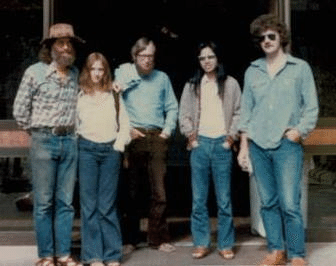
\includegraphics{graphics/lajolla_08_75.png}

}

\caption{Forrest Young, Bepi Pinner, Jean-Marie Bouroche, Yoshio Takane,
Jan de Leeuw at La Jolla, August 1975}

\end{figure}%

\bookmarksetup{startatroot}

\chapter*{Notation and Reserved
Symbols}\label{notation-and-reserved-symbols}
\addcontentsline{toc}{chapter}{Notation and Reserved Symbols}

\markboth{Notation and Reserved Symbols}{Notation and Reserved Symbols}

intro

\section*{Spaces}\label{spaces}
\addcontentsline{toc}{section}{Spaces}

\markright{Spaces}

\begin{itemize}
\item
  \(\mathbb{R}^n\) is the space of all real vectors, i.e.~all
  \(n\)-element tuples of real numbers. Typical elements of
  \(\mathbb{R}^n\) are \(x,y,z\). The element of \(x\) in position \(i\)
  is \(x_i\). Defining a vector by its elements is done with
  \(x=\{x_i\}\).
\item
  \(\mathbb{R}^n\) is equipped with the inner product
  \(\langle x,y\rangle=x'y=\sum_{i=1}^nx_iy_i\) and the norm
  \(\|x\|=\sqrt{x'x}\).
\item
  The canonical basis for \(\mathbb{R}^n\) is the \(n-\)tuple
  \((e_1,cdots,e_n)\), where \(e_i\) has element \(i\) equal to \(+1\)
  and all other elements equal to zero. Thus \(\|e_i\|=1\) and
  \(\langle e_i,e_j\rangle=\delta^{ij}\), with \(\delta^{ij}\) the
  Kronecker delta (equal to one if \(i=j\) and zero otherwise). Note
  that \(x_i=\langle e_i,x\rangle\).
\item
  \(\mathbb{R}\) is the real line and \(\mathbb{R}_+\) is the half line
  of non-negative numbers.
\item
  \(\mathbb{R}^{n\times m}\) is the space of all \(n\times m\) real
  matrices. Typical elements of \(\mathbb{R}^{n\times m}\) are
  \(A,B,C\). The element of \(A\) in row \(i\) and column \(j\) is
  \(a_{ij}\). Defining a matrix by its elements is done with
  \(A=\{a_{ij}\}\).
\item
  \(\mathbb{R}^{n\times m}\) is equipped with the inner product
  \(\langle A,B\rangle=\text{tr} A'B=\sum_{i=1}^n\sum_{j=1}^ma_{ij}b_{ij}\)
  and the norm \(\|A\|=\sqrt{\text{tr}\ A'A}\).
\item
  The canonical basis for \(\mathbb{R}^{n\times m}\) is the \(nm-\)tuple
  \((E_{11},cdots,E_{nm})\), where \(E_{ij}\) has element \((i,j)\)
  equal to \(+1\) and all other elements equal to zero. Thus
  \(\|E_{ij}\|=1\) and
  \(\langle E_{ij},E_{kl}\rangle=\delta^{ik}\delta^{jl}\).
\end{itemize}

\(\text{vec}\) and \(\text{vec}^{-1}\)

\section*{Matrices}\label{matrices}
\addcontentsline{toc}{section}{Matrices}

\markright{Matrices}

\begin{itemize}
\item
  \(a_{i\bullet}\) is row \(i\) of matrix \(A\), \(a_{\bullet j}\) is
  column \(j\).
\item
  \(a_{i\star}\) is the sum of row \(i\) of matrix \(A\),
  \(a_{\star j}\) is the sum of column \(j\).
\item
  \(A'\) is the transpose of \(A\), and \(\text{diag}(A)\) is the
  diagonal matrix with the diagonal elements of \(A\). The inverse of a
  square matrix \(A\) is \(A^{-1}\), the Moore-Penrose generalized
  inverse of any matrix \(A\) is \(A^+\).
\item
  If \(A\) and \(B\) are two \(n\times m\) matrices then their Hadamard
  (or elementwise) product \(C=A\times B\) has elements
  \(c_{ij}=a_{ij}b_{ij}\). The Hadamard quotient is \(C=A/B\), with
  elements \(c_{ij}=a_{ij}/b_{ij}\). The Hadamard power is
  \(A^{(k)}=A^{(p-1)}\times A\).
\item
  DC matrices. Centering matrix. \(J_n=I_n-n^{-1}E_n\). We do not use
  gthe subscripts if the order is obvious from the context.
\end{itemize}

\section*{Functions}\label{functions}
\addcontentsline{toc}{section}{Functions}

\markright{Functions}

\begin{itemize}
\item
  \(f,g,h,\cdots\) are used for functions or mappings.
  \(f:X\rightarrow Y\) says that \(f\) maps \(X\) into \(Y\).
\item
  \(\sigma\) is used for all real-valued least squares loss functions.
\end{itemize}

\section*{MDS}\label{mds}
\addcontentsline{toc}{section}{MDS}

\markright{MDS}

\begin{itemize}
\item
  \(\Delta=\{\delta_{ij\cdots}\}\) is a matrix or array of
  dissimilarities.
\item
  \(\langle \mathbb{X},d\rangle\) is a metric space, with
  \(d:\mathcal{X}\otimes\mathcal{X}\rightarrow\mathbb{R}_+\) the
  distance function. If \(X\) is is an ordered n-tuple
  \((x_1,\cdots,x_n)\) of elements of \(\mathcal{X}\) then \(D(X)\) is
  \(\{d(x_i,x_j)\}\), the elements of which we also write as
  \(d_{ij}(X)\).
\item
  Summation over the elements of vector \(x\in\mathbb{R}^n\) is
  \(\sum_{i=1}^n x_i\). Summation over the elements of matrix
  \(A\in\mathbb{R}^{n\times m}\) is \(\sum_{i=1}^n\sum_{j=1}^m a_{ij}\).
  Summation over the elements above the diagonal of \(A\) is
  \(\mathop{\sum\sum}_{1\leq i<j\leq n}a_{ij}\).
\item
  Conditional summation is, for example,
  \(\sum_{i=1}^n \{x_i\mid x_i>0\}\).
\end{itemize}

Iteration

\bookmarksetup{startatroot}

\chapter*{Preface}\label{preface}
\addcontentsline{toc}{chapter}{Preface}

\markboth{Preface}{Preface}

This book is definitely \emph{not} an impartial and balanced review of
all of multidimensional scaling (MDS) theory and history. It emphasizes
computation, and the mathematics needed for computation. In addition, it
is a summary of over 50 years of MDS work by me, either solo or together
with my many excellent current or former co-workers and co-authors. It
is heavily biased in favor of the smacof formulation of MDS (De Leeuw
(\citeproc{ref-deleeuw_C_77}{1977a}), De Leeuw and Heiser
(\citeproc{ref-deleeuw_heiser_C_77}{1977}), De Leeuw and Mair
(\citeproc{ref-deleeuw_mair_A_09c}{2009})), and the corresponding
majorization (or MM) algorithms. And, moreover, I am shamelessly
squeezing in as many references to my published and unpublished work as
possible, with links to the corresponding pdf's if they are available.
Thus this book is also a jumpstation into my bibliography.

I have not organized the book along historical lines because most of the
early techniques and results have been either drastically improved or
completely abandoned. Nevertheless, some personal historical perspective
may be useful. I will put most of it in this preface, so uninterested
readers can easily skip it.

I got involved in MDS in 1968 when John van de Geer returned from a
visit to Clyde Coombs in Michigan and started the Department of Data
Theory in the Division of Social Sciences at Leiden University. I was
John's first hire, although I was still a graduate student at the time.

Remember that Clyde Coombs was running the Michigan Mathematical
Psychology Program, and he had just published his remarkable book ``A
Theory of Data'' (Coombs (\citeproc{ref-coombs_64}{1964})). The name of
the new department in Leiden was taken from the title of that book, and
Coombs was one of the first visitors to give a guest lecture there.

This is maybe the place to clear up some possible misunderstandings
about the name ``Data Theory''. Coombs was mainly interested in a
taxonomy of data types, and in pointing out that ``data'' were not
limited to a table or data-frame of objects by variables. In addition,
there were also similarity ratings, paired comparisons, and unfolding
data. Coombs also emphasized that data were often non-metric,
i.e.~ordinal or categorical, and that it was possible to analyze these
ordinal or categorical relationships directly, without first
constructing numerical scales to which classical techniques could be
applied. One of the new techniques discussed in Coombs
(\citeproc{ref-coombs_64}{1964}) was a ordinal form of MDS, in which not
only the data but also the representation of the data in Euclidean space
were non-metric.

John van de Geer had just published Van de Geer
(\citeproc{ref-vandegeer_67}{1967}). In that book, and in the subsequent
book Van de Geer (\citeproc{ref-vandegeer_71}{1971}), he developed his
unique geometric approach to multivariate analysis. Relationship between
variables, and between variables and individuals, were not just
discussed using matrix algebra, but were also visualized in diagrams.
This was related to the geometric representations in Coombs' Theory of
Data, but it concentrated on numerical data in the form of rectangular
matrices of objects by variables.

Looking back it is easy to see that both Van de Geer and Coombs
influenced my approach to data analysis. I inherited the emphasis on
non-metric data and on visualization. But, from the beginning, I
interpreted ``Data Theory'' as ``Data Analysis'', with my emphasis
shifting to techniques, loss functions, implementations, algorithms,
optimization, computing, and programming. This is of interest because in
2020 my former Department of Statistics at UCLA, together with the
Department of Mathematics, started a bachelor's program in Data Theory,
in which ``Emphasis is placed on the development and theoretical support
of a statistical model or algorithmic approach. Alternatively, students
may undertake research on the foundations of data science, studying
advanced topics and writing a senior thesis.'' This sounds like a nice
hybrid of Data Theory and Data Analysis, with a dash of computer science
mixed in.

Computing and optimization were in the air in 1968, not so much because
of Coombs, but mainly because of Roger Shepard, Joe Kruskal, and Doug
Carroll at Bell Labs in Murray Hill. John's other student Eddie Roskam
and I were fascinated by getting numerical representations from ordinal
data by minimizing explicit least squares loss functions. Eddie wrote
his dissertation in 1968 (Roskam (\citeproc{ref-roskam_68}{1968})). In
1973 I went to Bell Labs for a year, and Eddie went to Michigan around
the same time to work with Jim Lingoes, resulting in Lingoes and Roskam
(\citeproc{ref-lingoes_roskam_73}{1973}).

My first semi-publication was De Leeuw
(\citeproc{ref-deleeuw_R_68g}{1968c}), quickly followed by a long
sequence of other, admittedly rambling, internal reports. Despite this
very informal form of publication the sheer volume of them got the
attention of Joe Kruskal and Doug Carroll, and I was invited to spend
the academic year 1973-1974 at Bell Laboratories. That visit somewhat
modified my cavalier approach to publication, but I did not become
half-serious in that respect until meeting with Forrest Young and Yoshio
Takane at the August 1975 US-Japan seminar on MDS in La Jolla. Together
we used the alternating least squares approach to algorithm construction
that I had developed since 1968 into a quite formidable five-year
publication machine, with at its zenith Takane, Young, and De Leeuw
(\citeproc{ref-takane_young_deleeuw_A_77}{1977}).

In La Jolla I gave the first presentation of the majorization method for
MDS, later known as smacof, with the first formal convergence proof. The
canonical account of smacof was published in a conference paper (De
Leeuw (\citeproc{ref-deleeuw_C_77}{1977a})). Again I did not bother to
get the results into a journal or into some other more effective form of
publication. The basic theory for what became known as smacof was also
presented around the same time in another book chapter De Leeuw and
Heiser (\citeproc{ref-deleeuw_heiser_C_77}{1977}).

In 1978 I was invited to the Fifth International Symposium on
Multivariate Analysis in Pittsburgh to present what became De Leeuw and
Heiser (\citeproc{ref-deleeuw_heiser_C_80}{1980}). There I met Nan
Laird, one of the authors of the basic paper on the EM algorithm
(Dempster, Laird, and Rubin
(\citeproc{ref-dempster_laird_rubin_77}{1977})). I remember
enthusiastically telling her on the conference bus that EM and smacof
were both special case of the general majorization approach to algorithm
construction, which was consequently born around the same time. But that
is a story for a companion volume, which currently only exists in a very
preliminary stage (https://github.com/deleeuw/bras).

My 1973 PhD thesis (De Leeuw (\citeproc{ref-deleeuw_B_73}{1973a}),
reprinted as De Leeuw (\citeproc{ref-deleeuw_B_84}{1984a})) was actually
my second attempt at a dissertation. I had to get a PhD, any PhD, before
going to Bell Labs, because of the difference between the Dutch and
American academic title and reward systems. I started writing a
dissertation on MDS, in the spirit of what later became De Leeuw and
Heiser (\citeproc{ref-deleeuw_heiser_C_82}{1982}). But halfway through I
lost interest and got impatient, and I decided to switch to nonlinear
multivariate analysis. This second attempt did produced a finished
dissertation (De Leeuw (\citeproc{ref-deleeuw_B_73}{1973a})), which grew
over time, with the help of multitudes, into Gifi
(\citeproc{ref-gifi_B_90}{1990}). But that again is a different history,
which I will tell some other time in yet another companion volume
(https://github.com/deleeuw/gifi). For a long time I did not do much
work on MDS, until the arrival of Patrick Mair and the R language led to
a resurgence of my interest, and ultimately to De Leeuw and Mair
(\citeproc{ref-deleeuw_mair_A_09c}{2009}) and Mair, Groenen, and De
Leeuw (\citeproc{ref-mair_groenen_deleeuw_A_22}{2022}).

I consider this MDS book to be a summary and extension of the basic
papers De Leeuw (\citeproc{ref-deleeuw_C_77}{1977a}), De Leeuw and
Heiser (\citeproc{ref-deleeuw_heiser_C_77}{1977}), De Leeuw and Heiser
(\citeproc{ref-deleeuw_heiser_C_80}{1980}), De Leeuw and Heiser
(\citeproc{ref-deleeuw_heiser_C_82}{1982}), and De Leeuw
(\citeproc{ref-deleeuw_A_88b}{1988}), all written 30-40 years ago.
Footprints in the sands of time. It can also be seen as an elaboration
of the more mathematical and computational sections of the excellent and
comprehensive textbook of Borg and Groenen
(\citeproc{ref-borg_groenen_05}{2005}). That book has much more
information about the origins, the data, and the applications of MDS, as
well as on the interpretation of MDS solutions. In this book I
concentrate almost exclusively on the mathematical, computational, and
programming aspects of MDS.

For those who cannot get enough of me, there is a data base of my
published and unpublished reports and papers since 1965, with links to
pdf's, at \url{https://jansweb.netlify.app/publication/}.

There are many, many people I have to thank for my scientific education.
Sixty years is a long time, and consequently many excellent teachers and
researchers have crossed my path. I will gratefully mention the
academics who had a major influence on my work and who are not with us
any more, since I will join them in the not too distant future: Louis
Guttman (died 1987), Clyde Coombs (died 1988), Warren Torgerson (died
1999), Forrest Young (died 2006), John van de Geer (died 2008), Joe
Kruskal (died 2010), Doug Carroll (died 2011), and Rod McDonald (died
2012).

\bookmarksetup{startatroot}

\chapter{Introduction}\label{intro}

In this book we study the smacof family of \emph{Multidimensional
Scaling (MDS)} techniques. In MDS the data consist of some type of
information about the \emph{dissimilarities} between a pairs of
\emph{objects}. These objects can be anything: individuals, variables,
colors, locations, chemicals, molecules, works of Plato, political
parties, Morse code signals, and so on. The dissimilarities can be
approximate or imprecise distances, dissimilarity judgments,
import/export tables, sociometric choices, and so on. They generally are
\emph{distance-like}, but we do not expect them to satisfy the triangle
inequality, and in general not even non-negativity and symmetry.
\emph{Similarities}, such as confusion probabilities, correlations, or
preferences, are always converted in some way or another to
dissimilarities before they can serve as data for MDS.

The information we have about these dissimilarities can be numerical,
ordinal, or categorical. Thus we may have the actual values of some or
all of the dissimilarities, we may know their rank order, or we may have
a classification of them into a small number of qualitative bins.

Let's formalize this, and introduce some notation at the same time. The
set of ojects is \(\mathfrak{O}\). For example, it can be the set of all
cities with more than 10,000 inhabitants. In our MDS analysis we only
use \(O:=(o_1,\cdots,o_n)\), an n-tuple (i.e.~a finite sequence) of
\(n\) \emph{different} elements of \(\mathfrak{O}\), for example \(n\)
capital cities selected from \(\mathfrak{O}\). If you want to, you can
call \(O\) a \emph{sample} from \(\mathfrak{O}\). It is entirely
possible, however, that \(\mathfrak{O}\) has only \(n\) elements, in
which case \(O\) is just an permutation of the elements of
\(\mathfrak{O}\).

A dissimilarity is a function \(\delta\) on all pairs of objects, with
values in a set \(\mathfrak{D}\). It can be, for example, the time in
seconds for an airline flight from city one to city two. Thus
\(\delta:\mathfrak{O}\otimes\mathfrak{O}\Rightarrow\mathfrak{D}\). A
dissimilaritry is \emph{numerical} if \(\mathfrak{D}\) is subset of real
line, it is \emph{ordinal} if \(\mathfrak{D}\) is a partially ordered
set, and it is \emph{nominal} if \(\mathfrak{D}\) is neither. Or a
dissimilarty is nominal if \(\mathfrak{D}\) is any set, and we choose to
ignore the ordinal and numerical information if it is there. No matter
what \(\mathfrak{D}\) is, we suppose it always has the element
\(\mathit{NA}\) to indicate missing dissimilarities. Cities may not have
airports, for example, or we just don't have the information about the
airline distances. Define \(\delta_{ij}:=\delta(o_i,o_j)\) and
\(\Delta:=\delta(O\times O)\). We can think of \(\Delta\) and an
\(n\times n\) matrix with elements in \(\mathfrak{D}\).

MDS techniques map the objects \(o_i\) into \emph{points} \(x_i\) in
some metric space \(\langle\mathfrak{X},d\rangle\) in such a way that
the distances between pairs of points approximate the dissimilarities of
the corresponding pairs of objects. Thus we want to find a map
\(x:\mathfrak{O}\rightarrow\mathfrak{X}\) that produces an n-tuple
\(X=(x_1,\cdots,x_n)\) of elements of \(\mathfrak{X}\), where
\(x_i:=x(o_i)\). Also define \(d_{ij}:=d(x_i,x_j)\) and
\(D(X):=d(X\times X\). Unlike the dissimilarities the \(d_{ij}\) are
always numerical, because distances are. So MDS finds \(X\) such that
\(D(X)\approx\Delta\).

For numerical dissimilarities it is clear what ``approximation'' means,
we simply want the distances and the corresponding dissimilarities to be
numerically close. Because there are generally many dissimilarities and
distances a combined measure of closeness can still be defined in many
different ways. For ordinal and nominal dissimilarities the notion of
approximation is less clear, and we have to develop more specialized
techniques to measure how well the distances fit the dissimilarities.

\section{Brief History}\label{introhist}

De Leeuw and Heiser (\citeproc{ref-deleeuw_heiser_C_80}{1980})

This section has a different emphasis. We limit ourselves to
developments in Euclidean MDS, and to contributions with direct
computational consequences that have a direct or indirect link to
psychometrics, and to work before 1960. This is reviewed ably in the
presidential address of W. S. Torgerson
(\citeproc{ref-torgerson_65}{1965}).

Our history review takes the form of brief summaries of what we consider
to be milestone papers or books.

\subsection{Milestones}\label{milestones}

W. S. Torgerson (\citeproc{ref-torgerson_52}{1952}) W. S. Torgerson
(\citeproc{ref-torgerson_65}{1965})

Shepard (\citeproc{ref-shepard_62a}{1962a}) Shepard
(\citeproc{ref-shepard_62b}{1962b})

Kruskal (\citeproc{ref-kruskal_64a}{1964a}) Kruskal
(\citeproc{ref-kruskal_64b}{1964b})

Guttman (\citeproc{ref-guttman_68}{1968})

De Leeuw (\citeproc{ref-deleeuw_C_77}{1977a}) De Leeuw and Heiser
(\citeproc{ref-deleeuw_heiser_C_77}{1977})

There was some early work by Richardson, Messick, Abelson and Torgerson
who combined Thurstonian scaling of similarities with the mathematical
results of Schoenberg (\citeproc{ref-schoenberg_35}{1935}) and G. Young
and Householder (\citeproc{ref-young_householder_38}{1938}).

Despite these early contributions it makes sense, certainly from the
point of view of my personal history, but probably more generally, to
think of MDS as starting as a widely discussed, used, and accepted
technique since the book by W. S. Torgerson
(\citeproc{ref-torgerson_58}{1958}). This was despite the fact that in
the fifties and sixties computing eigenvalues and eigenvectors of a
matrix of size 20 or 30 was still a considerable challenge.

A few years later the popularity of MDS got a large boost by
developments centered at Bell Telephone Laboratories in Murray Hill, New
Jersey, the magnificent precursor of Silicon Valley. First there was
nonmetric MDS by Shepard (\citeproc{ref-shepard_62a}{1962a}), Shepard
(\citeproc{ref-shepard_62b}{1962b}) and Kruskal
(\citeproc{ref-kruskal_64a}{1964a}), Kruskal
(\citeproc{ref-kruskal_64b}{1964b}), And later another major development
was the introduction of individual difference scaling by Carroll and
Chang (\citeproc{ref-carroll_chang_70}{1970}) and Harshman
(\citeproc{ref-harshman_70}{1970}). Perhaps even more important was the
development of computer implementations of these new techniques. Some of
the early history of nonmetric MDS is in De Leeuw
(\citeproc{ref-deleeuw_E_17e}{2017e}).

Around the same time there were interesting theoretical contributions in
Coombs (\citeproc{ref-coombs_64}{1964}), which however did not much
influence the practice of MDS. \ldots.. And several relatively minor
variations of the Bell Laboratories approach were proposed by Guttman
(\citeproc{ref-guttman_68}{1968}), but Guttman's influence on further
MDS implementations turned out to be fairly localized and limited.

The main development in comptational MDS after the Bell Laboratories
surge was probably smacof. Initially, in De Leeuw
(\citeproc{ref-deleeuw_C_77}{1977a}), this stood for \emph{Scaling by
Maximizing a Convex Function}. Later it was also used to mean
\emph{Scaling by Majorizing a Complicated Function}. Whatever. In this
book smacof just stands for smacof. No italics, no boldface, no
capitals.

The first smacof programs were written in 1977 in FORTRAN at the
Department of Data Theory in Leiden (Heiser and De Leeuw
(\citeproc{ref-heiser_deleeuw_R_77}{1977})). Eventually they migrated to
SPSS (for example, Meulman and Heiser
(\citeproc{ref-meulman_heiser_12}{2012})) and to R (De Leeuw and Mair
(\citeproc{ref-deleeuw_mair_A_09c}{2009})). The SPSS branch and the R
branch have diverged somewhat, and they continue to be developed
independently.

Parallel to this book there is an attempt to rewrite the various smacof
programs in C, with the necessary wrappers to call them from R (De Leeuw
(\citeproc{ref-deleeuw_E_17p}{2017f})). The C code, with makefiles and
test routines, is at
\href{https://github.com/deleeuw/smacof}{github.com/deleeuw/smacof}

\section{Basic MDS}\label{introbasic}

Following Kruskal, and to a lesser extent Shepard, we measure the fit of
distances to dissimilarities using an explicit real-valued \emph{loss
function} (or \emph{badness-of-fit measure}), which is minimized over
the possible maps of the objects into the metric space. This is a very
general definition of MDS, covering all kinds of variations of the
target metric space and of the way fit is measured. Obviously we will
not discuss \emph{all} these possible forms of MDS, which also includes
various techniques more properly discussed as cluster analysis,
classification, or discrimination.

To fix our scope we first define \emph{basic MDS}, which is short for
\emph{Least Squares Euclidean Metric MDS}. It is defined as MDS with the
following characteristics.

\begin{enumerate}
\def\labelenumi{\arabic{enumi}.}
\tightlist
\item
  The metric space is a Euclidean space.
\item
  The dissimilarities are numerical, symmetric, and non-negative.
\item
  The loss function is a weighted sum of squares of the
  \emph{residuals}, which are the differences between dissimilarities
  and Euclidean distances.
\item
  Weights are numerical, symmetric, and non-negative.
\item
  Self-dissimilarities are zero and the corresponding terms in the loss
  function also have weight zero.
\end{enumerate}

By a \emph{Euclidean space} we mean a finite dimensional vector space,
with addition and scalar multiplication, and with an inner product that
defines the distances. For the \emph{inner product} of vectors \(x\) and
\(y\) we write \(\langle x,y\rangle\). The \emph{norm} of \(x\) is
defined as \(\|x\|:=\sqrt{\langle x,x\rangle}\), and the \emph{distance}
between \(x\) and \(y\) is \(d(x,y):=\|x-y\|\).

The \emph{loss function} we use is called \emph{stress}. It was first
explicitly introduced in MDS as \emph{raw stress} by Kruskal
(\citeproc{ref-kruskal_64a}{1964a}) and Kruskal
(\citeproc{ref-kruskal_64b}{1964b}). We define stress in a slightly
different way, because we want to be consistent over the whole range of
the smacof versions and implementations. In smacof stress is the
real-valued function \(\sigma\), defined on the space
\(\mathbb{R}^{n\times p}\) of configurations, as

\begin{equation}\phantomsection\label{eq-stressall}{
\sigma(X):=\frac14\sum_{i=1}^n\sum_{j=1}^n w_{ij}(\delta_{ij}-d_{ij}(X))^2.
}\end{equation}

Note that we use \(:=\) for definitions, i.e.~for concepts and symbols
that are not standard mathematical usage, when they occur for the first
time in this book. Through the course of the book it will probably
become clear why the mysterious factor \(\frac14\) is there. Clearly it
has no influence on the actual minimization of the loss function.

In Equation~\ref{eq-stressall} we use the following objects and symbols.

\begin{enumerate}
\def\labelenumi{\arabic{enumi}.}
\tightlist
\item
  \(W=\{w_{ij}\}\) is a symmetric, non-negative, and hollow matrix of
  \emph{weights}, where \emph{hollow} means zero diagonal.
\item
  \(\Delta=\{\delta_{ij}\}\) is a symmetric, non-negative, and hollow
  matrix of \emph{dissimilarities}.
\item
  \(X\) is an \(n\times p\) \emph{configuration}, containing coordinates
  of \(n\) \emph{points} in \(p\) dimensions.
\item
  \(D(X)=\{d_{ij}(X)\}\) is a symmetric, non-negative, and hollow matrix
  of \emph{Euclidean distances} between the \(n\) points in \(X\). Thus
  \(d_{ij}(X):=\sqrt{\sum_{s=1}^p(x_{is}-x_{js})^2}\).
\end{enumerate}

Note that symmetry and hollowness of the basic objects \(W\),
\(\Delta\), and \(D\) allows us carry out the summation of the weighted
squared residuals in formula (Equation~\ref{eq-stressall}) over the
upper (or lower) diagonal elements only. Thus we can also write
\begin{equation}\phantomsection\label{eq-stresshalf}{
\sigma(X):=\frac12\mathop{\sum\sum}_{1\leq i<j\leq n} w_{ij}(\delta_{ij}-d_{ij}(X))^2.
}\end{equation} We use the notation
\(\mathop{\sum\sum}_{1\leq i<j\leq n}\) for summation over the
lower-diagonal elements of a matrix.

The function \(D\), which computes the distance matrix \(D(X)\) from a
configuration \(X\), is matrix-valued. It maps the
\(n\times p\)-dimensional \emph{configuration space}
\(\mathbb{R}^{n\times p}\) into the set \(D(\mathbb{R}^{n\times p})\) of
Euclidean distance matrices between \(n\) points in \(\mathbb{R}^p\),
which is a subset of the convex cone of hollow, symmetric, non-negative
matrices in the linear space \(\mathbb{R}^{n\times n}\) (Datorro
(\citeproc{ref-datorro_18}{2018})).

In basic MDS the weights and dissimilarities are given numbers, and we
minimize stress over all \(n\times p\) configurations \(X\). Note that
the \emph{dimensionality} \(p\) is also supposed to be known beforehand,
and that MDS in \(p\) dimensions is different from MDS in \(q\not= p\)
dimensions. We sometimes emphasize this by writing \(pMDS\), which
indicates that we will map the points into \(p\)-dimensional space.

Two boundary cases that will interest us are \emph{Unidimensional
Scaling} or \emph{UDS}, where \(p=1\), and \emph{Full-dimensional
Scaling} or \emph{FDS}, where \(p=n\). Thus UDS is 1MDS and FDS is nMDS.
Most actual MDS applications in the sciences use 1MDS, 2MDS or 3MDS,
because configurations in one, two, or three dimensions can easily be
plotted with standard graphics tools. Note that MDS is not primarily a
tool to tests hypotheses about dimensionality and to find meaningful
dimensions. It is a mostly a mapping tool for data reduction, to
graphically find interesting aspects of dissimilarity matrices.

The projections on the dimensions are usually ignored, it is the
configuration of points that is the interesting outcome. This
distinguishes MDS from, for example, factor analysis. There is no
Varimax, Oblimax, Quartimax, and so on. Exceptions are confirmatory
applications of MDS in genetic mapping along the chromosome, in
archeological seriation, in testing psychological theories of cognition
and representation, in the conformation of molecules, and in geographic
and geological applications. In these areas the dimensionality and
general structure of the configuration are given by prior knowledge, we
just do not know the precise location and distances of the points. For
more discussion of the different uses of MDS we refer to De Leeuw and
Heiser (\citeproc{ref-deleeuw_heiser_C_82}{1982}).

\subsection{Kruskal's stress}\label{kruskals-stress}

Equation~\ref{eq-stressall} differs from Kruskal's original stress in at
least three ways: in Kruskal's use of the square root, in our use of
weights, and in our different approach to normalization.

We have paid so much attention to Kruskal's original definition, because
the choices made there will play a role in the normalization discussion
in the ordinal scaling chapter (section \textbf{?@sec-nmdsnorm}), in the
comparison of Kruskal's and Guttman's approach to ordinal MDS (sections
@ref(nmdskruskal) and @ref(nmdsguttman)), and in our discussions about
the differences between Kruskal's stress @ref(eq:kruskalstressfinal) and
smacof's stress @ref(eq:stressall) in the next three sections of this
chapter.

\subsubsection{Square root}\label{square-root}

Let's discuss the square root first. Using it or not using it does not
make a difference for the minimization problem. Using the square root,
however, does give a more sensible root-mean-square scale, in which
stress is homogeneous of degree one, instead of degree two. But I do not
want to compute all those unnecessary square roots in my algorithms, and
I do not want to drag them along through my derivations. Moreover the
square root potentially causes problems with differentiability at those
\(X\) where \(\sigma(X)\) is zero. Thus, througout the book, we do not
use the square root in our formulas and derivations. In fact, we do not
even use it in our computer programs, except at the very last moment
when we return the final stress after the algorithm has completed.

\subsubsection{Weights}\label{bweights}

There were no weights \(W=\{w_{ij}\}\) in the original definition of
stress by Kruskal (\citeproc{ref-kruskal_64a}{1964a}), and neither are
they there in most of the basic later contributions to MDS by Guttman,
Lingoes, Roskam, Ramsay, or Young. We will use weights throughout the
book, because they have various interesting applications within basic
MDS, without unduly complicating the derivations and computations. In
Groenen and Van de Velden (\citeproc{ref-groenen_vandevelden_16}{2016}),
section 6, the various uses of weights in the stress loss function are
enumerated. They generously, but correctly, attribute the consistent use
of weights in MDS to me. I quote from their paper:

\begin{quote}
\begin{enumerate}
\def\labelenumi{\arabic{enumi}.}
\tightlist
\item
  Handling missing data is done by specifying \(w_{ij} = 0\) for
  missings and 1 otherwise thereby ignoring the error corresponding to
  the missing dissimilarities.
\item
  Correcting for nonuniform distributions of the dissimilarities to
  avoid dominance of the most frequently occurring dissimilarities.
\item
  Mimicking alternative fit functions for MDS by minimizing Stress with
  \(w_{ij}\) being a function of the dissimilarities.
\item
  Using a power of the dissimilarities to emphasize the fitting of either
  large or small dissimilarities.
\item
  Special patterns of weights for specific models.
\item
  Using a specific choice of weights to avoid nonuniqueness.
\end{enumerate}
\end{quote}

In some situations, for example for huge data sets, it is
computationally convenient, or even necessary, to minimize the influence
of the weights on the computations. We can use \emph{majorization} to
turn the problem from a weighted least squares problem to an iterative
unweighted least squares problem. The technique, which we call
\emph{unweighting}, is discussed in detail in section @ref(minunweight).

\subsubsection{Normalization}\label{intronorm}

This section deals with a rather trivial problem, which has however
caused problems in various stages of smacof's 45-year development
history. Because the problem is trivial, and the choices that must be
made are to a large extent arbitrary, it has been overlooked and
somewhat neglected.

In basic MDS we scale the weights and dissimilarities. It is clear that
if we multiply the weights or dissimilarities by a constant, then the
optimal approximating distances \(D(X)\) and the optimal configuration
\(X\) will be multiplied by the same constant. That is exactly why
Kruskal's raw stress had to be normalized. Consequently we in basic MDS
we always scale weights and dissimilarities by

\begin{align}
\mathop{\sum\sum}_{1\leq i<j\leq n}w_{ij}&=1,(\#eq:scaldiss1)\\
\mathop{\sum\sum}_{1\leq i<j\leq n}w_{ij}^{\ }\delta_{ij}^2&=1.(\#eq:scaldiss2)
\end{align}

This simplifies our formulas and makes them look better (see, for
example, section @ref(propexpand) and section @ref(secrhostress)). It
presupposes, of course, that \(w_{ij}\delta_{ij}\not=0\) for at least
one \(i\not= j\), which we will happily assume in the sequel, because
otherwise the MDS problem is trivial. Note that if all weights are equal
(which we call the \emph{unweighted case}) then they are equal to
\(1/\binom{n}{2}\) and thus we require
\(\mathop{\sum\sum}_{1\leq i<j\leq n}\delta_{ij}^2=\frac12n(n-1)\).

Using normalized dissimilarities amounts to the same defining stress as

\begin{equation}
\sigma(X)=\frac12\frac{\mathop{\sum\sum}_{1\leq i<j\leq n}w_{ij}(\delta_{ij}^2-d_{ij}(X))^2}{\mathop{\sum\sum}_{1\leq i<j\leq n}w_{ij}\delta_{ij}^2}.
(\#eq:stressrat)
\end{equation}

This is useful to remember when we discuss the various normalizations
for non-metric MDS in section @ref(nmdsnorm).

\section{Local and Global}\label{seclocglob}

In basic MDS our goal is to compute both \(\min_X\sigma(X)\) and
\(\mathop{\text{Argmin}}_X\sigma(X)\), where \(\sigma(X)\) is defined as
@ref(eq:stressall), and where we minimize over all configurations in
\(\mathbb{R}^{n\times p}\).

In this book we study both the properties of the stress loss function
and a some of its generalizations, and the various ways to minimize
these loss functions over configurations (and sometimes over
transformations of the dissimilarities as well).

Emphasis local minima

Compute stationary points

Note we use the notation \(\mathop{\text{Argmin}}_{x\in X}f(x)\) for the
set of minimizers of \(f\) over \(X\). Thus
\(z\in\mathop{\text{Argmin}}_{x\in X}f(x)\) means \(z\) minimizes \(f\)
over \(X\), i.e.~\(f(z)=\min_{x\in X} f(x)\). If it is clear from theory
that the minimum is necessarily unique, we use \(\text{argmin}\) instead
of \(\text{Argmin}\).

\section{Generalizations}\label{introgeneralize}

The most important generalizations of basic MDS we will study in later
chapters of this book are discussed briefly in the following sections.

\subsection{Non-metric MDS}\label{gennonmetric}

Basic MDS is a form of \emph{Metric Multidimensional Scaling} or
\emph{MMDS}, in which dissimilarities are either known or missing. In
chapter @ref(nonmtrmds) we relax this assumption. Dissimilarities may be
partly known, for example we may know they are in some interval, we may
only know their order, or we may know them up to some smooth
transformation. MDS with partly known dissimilarities is
\emph{Non-metric Multidimensional Scaling} or \emph{NMDS}. Completely
unknown (missing) dissimilarities are an exception, because we can just
handle this in basic MDS by setting the corresponding weights equal to
zero.

In NMDS we minimize stress over all configurations, but also over the
unknown dissimilarities. What we know about them (the interval they are
in, the transformations that are allowed, the order they are in) defines
a subset of the space of non-negative, hollow, and symmetric matrices.
Any matrix in that subset is a matrix of what Takane, Young, and De
Leeuw (\citeproc{ref-takane_young_deleeuw_A_77}{1977}) call
\emph{disparities}, i.e.~imputed dissimilarities. The imputation
provides the missing information and transforms the non-numerical
information we have about the dissimilarities into a numerical matrix of
disparities. Clearly this is an \emph{optimistic imputation}, in the
sense that it chooses from the set of admissible disparities to minimize
stress (for a given configuration).

One more terminological point. Often \emph{non-metric} is reserved for
ordinal MDS, in which we only know a (partial or complete) order of the
dissimilarities. Allowing linear or polynomial transformations of the
dissimilarities, or estimating an additive constant, is then supposed to
be a form of metric MDS. There is something to be said for that. Maybe
it makes sense to distinguish non-metric \emph{in the wide sense} (in
which stress must be minimized over both \(X\) and \(\Delta\)) and
\emph{non-metric in the narrow sense} in which the set of admissible
disparities is defined by linear inequalities. Nonmetric in the narrow
sense will also be called \emph{ordinal MDS} or \emph{OMDS}.

It is perhaps useful to remember that Kruskal
(\citeproc{ref-kruskal_64a}{1964a}) introduced explicit loss functions
in MDS to put the somewhat heuristic NMDS techniques of Shepard
(\citeproc{ref-shepard_62a}{1962a}) onto a firm mathematical and
computational foundation. Thus, more or less from the beginning of
iterative least squares MDS, there was a focus on non-metric rather than
metric MDS, and this actually contributed a great deal to the magic and
success of the technique. In this book most of the results are derived
for basic MDS, which is metric MDS, with non-metric MDS as a relatively
straightforward extension not discussed until chapter @ref(nonmtrmds).
So, at least initially, we take the numerical values of the
dissimilarities seriously, as do W. S. Torgerson
(\citeproc{ref-torgerson_58}{1958}) and Shepard
(\citeproc{ref-shepard_62a}{1962a}), Shepard
(\citeproc{ref-shepard_62b}{1962b}).

It may be the case that in the social and behavioural sciences only the
ordinal information in the dissimilarities is reliable and useful. But,
since 1964, MDS has also been applied in molecular conformation,
chemometrics, genetic sequencing, archelogical seriation, and in network
design and location analysis. In these areas the numerical information
in the dissimilarities is usually meaningful and should not be thrown
out right away. Also, the use of the Shepard plot, with dissimilarities
on the horizontal axis and fitted distances on the vertical axis,
suggests there is more to dissimilarities than just their rank order.

\subsection{fstress}\label{genfstress}

Instead of defining the residuals in the least squares loss function as
\(\delta_{ij}-d_{ij}(X)\) chapter @ref(chrstress) discusses the more
general cases where the residuals are \(f(\delta_{ij})-f(d_{ij}(X))\)
for some known non-negative increasing function \(f\). This defines the
\emph{fstress} loss function.

If \(f(x)=x^r\) with \(r>0\) then fstress is called \emph{rstress}. Thus
stress is rstress with \(r=1\), also written as \emph{1stress} or
\(\sigma_1\). In more detail we will also look at \(r=2\), which is
called \emph{sstress} by Takane, Young, and De Leeuw
(\citeproc{ref-takane_young_deleeuw_A_77}{1977}). In chapter
@ref(chsstressstrain) we look at the problem of minimizing sstress and
weighted version \emph{strain}. The case of rstress with
\(r\rightarrow 0\) is also of interest, because it leads to the loss
function in Ramsay (\citeproc{ref-ramsay_77}{1977}).

\subsection{Constraints}\label{gencons}

Instead of minimizing stress over all \(X\) in
\(\mathbb{R}^{n\times p}\) we will look in chapter @ref(cmds) at various
generalizations where minimization is over a subset \(\mathcal{\Omega}\)
of \(\mathbb{R}^{n\times p}\). This is often called \emph{Constrained
Multidimensional Scaling} or \emph{CMDS}.

The distinction may be familiar from factor analysis, where we
distinguish between exploratory and confirmatory factor analysis. If we
have prior information about the parameters then incorporating that
prior information in the analysis will generally lead to more precise
and more interpretable estimates. The risk is, of course that if our
prior information is wrong, if it is just prejudice, then we will have a
solution which is precise but incorrect. We have the famous trade-off
between bias and variance. In MDS this trade-off does not seem to apply
directly, because the necessary replication frameworks are missing.

and we do not attach much value to locating the true configuration.

\[
\min_{X\in\Omega}\sigma(X)
\]

\[
\min_X\sigma(X)+\lambda\kappa(X,\Omega)
\] where \(\kappa(X,\Omega)\geq 0\) and \(\kappa(X,\Omega)=0\) if and
only if \(X\in\Omega\).

\subsection{Individual Differences}\label{inreplic}

Now consider the situation in which we have \(m\) different
dissimilarity matrices \(\Delta_k\) and \(m\) different weight matrices
\(W_k\). We generalize basic MDS by defining \begin{equation}
\sigma(X_1,\cdots,X_m):=\frac12\sum_{k=1}^m\mathop{\sum\sum}_{1\leq i<j\leq n}w_{ijk}(\delta_{ijk}-d_{ij}(X_k))^2,
(\#eq:replistress)
\end{equation} and minimize this over the \(X_k\).

There are two simple ways to deal with this generalization. The first is
to put no further constraints on the \(X_k\). This means solving \(m\)
separate basic MDS problems, one for each \(k\). The second way is to
require that all \(X_k\) are equal. As shown in more detail in section
@ref(indifrepl) this reduced to a single basic MDS problem with
dissimilarities that are a weighted sum of the \(\Delta_k\). So both
these approaches do not really bring anything new.

Minimizing @ref(eq:replistress) becomes more interesting if we constrain
the \(X_k\) in various ways. Usually this is done by making sure they
have a component that is common to all \(k\) and a component that is
specific or unique to each \(k\). This approach, which generalizes
constrained MDS, is discussed in detail in chapter @ref(chindif).

\subsection{Distance Asymmetry}\label{genasym}

We have seen in section @ref(datasym) of this chapter that in basic MDS
the assumption that \(W\) and \(\Delta\) are symmetric and hollow can be
made without loss of generality. The simple partitioning which proved
this was based on the fact that \(D(X)\) is always symmetric and hollow.
By the way, the assumption that \(W\) and \(D\) are non-negative cannot
be made without loss of generality, as we will see below.

In chapter @ref(asymmds) we relax the assumption that \(D(X)\) is
symmetric (still requiring it to be non-negative and hollow). This could
be called \emph{Asymmetric MDS}, or \emph{AMDS}. I was reluctant at
first to include this chapter, because asymmetric distances do not
exist. And certainly are not Euclidean distances, so they are not
covered by the title of this book. But as long as we stay close to
Euclidean distances, least squares, and the smacof approach, I now feel
reasonably confident the chapter is not too much of a foreign body.

When Kruskal introduced gradient-based methods to minimize stress he
also discussed the possibility to use Minkovski metrics other than the
Euclidean metric. This certainly was part of the appeal of the new
methods, in fact it seemed as if the gradient methods made it possible
to use any distance function whatsoever. This initial feeling of
empowerment was somewhat naive, because it ignored the seriousness of
the local minimum problem, the combinatorial nature of one-dimensional
and city block scaling, the problems with nonmetric unfolding, and the
problematic nature of gradient methods if the distances are not
everywhere differentiable. All these complications will be discussed in
this book. But it made me decide to ignore Minkovski distances (and
hyperbolic and elliptic non-Euclidean distances), because life with
stress is complicated and challenging enough as it is.

\section{Models and Techniques}\label{models-and-techniques}

Truth, error

\bookmarksetup{startatroot}

\chapter{Properties of Stress}\label{propchapter}

\section{Notation}\label{propnotation}

The notation used in the \(\textrm{smacof}\) approach to MDS first
appeared in De Leeuw (\citeproc{ref-deleeuw_C_77}{1977a}), and was
subsequently used in several of the later key smacof references, such as
De Leeuw and Heiser (\citeproc{ref-deleeuw_heiser_C_82}{1982}), De Leeuw
(\citeproc{ref-deleeuw_A_88b}{1988}), chapter 8 of Borg and Groenen
(\citeproc{ref-borg_groenen_05}{2005}), and De Leeuw and Mair
(\citeproc{ref-deleeuw_mair_A_09c}{2009}). We follow it in this book.

\subsection{Expanding}\label{propexpand}

We expand stress by writing out the squares of the residuals and then
summing. Define

\begin{align}
\eta_\delta^2&:=\mathop{\sum\sum}_{1\leq i<j\leq n}w_{ij}\delta_{ij}^2,(\#eq:comps1)\\
\rho(X)&:=\mathop{\sum\sum}_{1\leq i<j\leq n}w_{ij}\delta_{ij}d_{ij}(X),(\#eq:comps2)\\
\eta^2(X)&:=\mathop{\sum\sum}_{1\leq i<j\leq n}w_{ij}d_{ij}^2(X).(\#eq:comps3)
\end{align}

More precisely, using conditional summation,

\begin{align}
\rho(X)&:=\mathop{\sum\sum}_{1\leq i<j\leq n}\left\{w_{ij}\delta_{ij}d_{ij}(X)\mid w_{ij}\delta_{ij}>0\right\},(\#eq:compszero1)\\
\eta^2(X)&:=\mathop{\sum\sum}_{1\leq i<j\leq n}\left\{w_{ij}d_{ij}^2(X)\mid w_{ij}>0\right\}(\#eq:compszero2).
\end{align}

Remember that we have normalized by \(\eta_\delta^2=1\). With our newly
defined functions \(\rho\) and \(\eta^2\) we can write stress as

\begin{equation}
\sigma(X)=\frac12(1+\eta^2(X))-\rho(X).
(\#eq:expand)
\end{equation}

The CS inequality implies that for all \(X\)

\begin{equation}
\rho(X)=\mathop{\sum\sum}_{1\leq i<j\leq n}w_{ij}\delta_{ij}d_{ij}(X)\leq\eta_\delta\eta(X)=\eta(X),
(\#eq:propcsrhoeta)
\end{equation}

and thus, from @ref(eq:expand),

\begin{align}
&\frac12(1-\eta(X))^2\leq\sigma(X)\leq\frac12(1+\eta^2(X)),(\#eq:propcssigeta1)\\
&\frac12(1-\rho(X))^2\leq\sigma(X)\leq\frac12(1-2\rho(X)).(\#eq:propcssigeta2)
\end{align}

\subsection{Matrix Expressions}\label{propmatrix}

Using matrix notation allows us to arrive at compact expressions, which
suggest various mathematical and computational shortcuts. In order to
use matrix notation for distances we mainly rely on the difference
matrices \(A_{ij}\), which we now define.

\begin{itemize}
\item
  A \emph{unit vector} \(e_i\) is a vector with element \(i\) equal to
  \(+1\) and all other elements equal to 0. A \emph{unit matrix}
  \(E_{ij}\) is a matrix of the form \(e_i^{\ }e_j'\),
\item
  A \emph{diff matrix} \(A_{ij}\) is a matrix of the form
  \((e_i-e_j)(e_i-e_j)'\).
\end{itemize}

The element in row \(i\) and column \(j\) of a matrix \(X\) is normally
referred to as \(x_{ij}\). But in some cases, to prevent confusion, we
use the notation \(\{X\}_{ij}\). Thus, for example,
\(\{e_i\}_j=\delta^{ij}\), where \(\delta^{ij}\) is \emph{Kronecker's
delta} (zero when \(i=j\) and one otherwise).

The diff matrices \(A_{ij}\) with \(i\not= j\) have only four non-zero
elements

\begin{align}
\begin{split}
\{A_{ij}\}_{ii}&=\{A_{ij}\}_{jj}=+1,\\
\{A_{ij}\}_{ij}&=\{A_{ij}\}_{ji}=-1,
\end{split}
(\#eq:apaele)
\end{align}

and all other elements of \(A_{ij}\) are zero. Thus \(A_{ij}=A_{ji}\)
and \(A_{ii}=0\). Diff matrices are symmetric, and positive
semidefinite. They are also \emph{doubly-centered}, which means that
their rows and columns add up to zero. If \(i\not j\) they are of rank
one and have one eigenvalue equal to two, which means
\(A_{ij}^s=2^{s-1}A_{ij}\). Also

\begin{equation}
\mathop{\sum\sum}_{1\leq i<j\leq n} A_{ij}=nI-ee'=nJ,
(\#eq:asum)
\end{equation}

with \(J\) the centering matrix.

We begin our matrix expressions with
\(d_{ij}^2(X)=\text{tr}\ X'A_{ij}X\). Define

\begin{equation}
V:=\mathop{\sum\sum}_{1\leq i<j\leq n}w_{ij}A_{ij},
(\#eq:vdef)
\end{equation}

so that

\begin{equation}
\eta^2(X)=\text{tr}\ X'VX.
(\#eq:etav)
\end{equation}

The matrix \(V\) has off-diagonal elements equal to \(-w_{ij}\) and
diagonal elements \(v_{ii}=\sum_{j\not= i} w_{ij}\) It is symmetric,
positive semi-definite, and doubly-centered. Thus it is singular,
because \(Ve=0\).

To analyze the singularity of \(V\) in more detail we observe that
\(z'Vz=\mathop{\sum\sum}_{1\leq i<j\leq n}w_{ij}(z_i-z_j)^2\). This is
zero if and only if all \(w_{ij}(z_i-z_j)^2\) are zero. If we permute
the elements of \(z\) such that \(z_1\leq\cdots\leq z_n\) then the
matrix with elements \((z_i-z_j)^2\) can be partitioned such that the
diagonal blocks, corresponding with tie-blocks in \(z\), are zero and
the off-diagonal blocks are strictly positive. Thus \(z'Vz=0\) if and
only if the corresponding off-diagonal blocks of \(W\) are zero. In
other words, we can find a \(z\) such that \(z'Vz=0\) if and only if
\(W\) is the direct sum of a number of smaller matrices. If this is not
the case we call \(W\) \emph{irreducible}, and \(z'Vz>0\) for all
\(z\not= e\), so that the rank of \(V\) is \(n-1\).

If \(W\) is reducible the MDS problem separates into a number of smaller
independent MDS problems. We will assume in the sequel, without any real
loss of generality, that this does not occur, and that consequently
\(W\) is irreducible.

Because of the singularity of the matrices involved we sometimes have to
work with generalized inverses. We limit ourselves to the Moore-Penrose
(MP) inverse, which can be defined in terms of the singular value
decomposition. If the singular value decomposition is \(X=K\Lambda L'\)
with \(K'K=L'L=I_r\) and \(\Lambda\) a positive definite diagonal matrix
of order \(r=\text{rank}(X)\), then the MP inverse of \(X\) is
\(X^+=L\Lambda^{-1}K'\).

Because of irreducibility the MP inverse of \(V\) is \begin{equation}
V^+=(V+\frac{ee'}{n})^{-1}-\frac{ee'}{n}.
(\#eq:mpv)
\end{equation} If all weights are equal, say to \(w\), then \(V=nwJ\)
and \(V^+=\frac{1}{nw}J\), with \(J\) the centering matrix
\(I-\frac{1}{n}ee'\).

Finding an expression for \(\rho(X)\) from @ref(eq:comps2) in matrix
form is a bit more complicated. Define \begin{equation}
r_{ij}(X):=\begin{cases}0&\text{ if }d_{ij}(X)=0,\\
\frac{\delta_{ij}}{d_{ij}(X)}&\text{ if }d_{ij}(X)>0,
\end{cases}
(\#eq:rdef)
\end{equation} and \begin{equation}
B(X):=\mathop{\sum\sum}_{1\leq i<j\leq n}w_{ij}r_{ij}(X)A_{ij}.
(\#eq:bdef)
\end{equation} Then we have \begin{equation}
\rho(X)=\text{tr}\ X'B(X)X.
(\#eq:rhob)
\end{equation} Just like \(V\), the matrix-valued function \(B\) is
symmetric, positive-semidefinite, and doubly-centered. If all
dissimilarities and distances are positive then irreducibility of \(W\)
implies that the rank of \(B(X)\) is equal to \(n-1\). Note that if
\(\delta_{ij}=d_{ij}(X)>0\) for all \(i,j\) (perfect fit), then the
\(r_{ij}\) from @ref(eq:rdef) are all equal to one, and \(B(X)=V\).

In @ref(eq:rdef) we have set \(r_{ij}(X)=0\) if \(d_{ij}(X)=0\). This is
arbitrary. Since \(b_{ij}(X)=r_{ij}(X)\) if \(d_{ij}(X)=0\) we get a
different matrix \(B(X)\) if we choose to set, say, \(r_{ij}(X)=1\) or
\(r_{ij}(X)=\delta_{ij}\) whenever \(d_{ij}(X)=0\). But \begin{equation}
B(X)X=\mathop{\sum\sum}_{1 \leq i<j\leq n}w_{ij}r_{ij}(X)(e_i-e_j)(x_i-x_j)'
(\#eq:propbinvar)
\end{equation} remains the same, no matter how we choose \(r_{ij}(X)\)
for the \(i<j\) with \(d_{ij}(X)=0\). And, consequently,
\(\rho(X)=\text{tr}\ X'B(X)X\) remains the same as well.

We now see, from equation @ref(eq:expand), that \begin{equation}
\sigma(X)=1-\ \text{tr}\ X'B(X)X+\frac12\text{tr}\ X'VX.
(\#eq:propmatexp)
\end{equation}

\subsection{Coefficient Space}\label{propcoefspace}

Observe that we distinguish configuration space, which is the linear
space \(\mathbb{R}^{n\times p}\) of \(n\times p\) matrices, from the
linear space \(\mathbb{R}^{np}\) of \(np\) element vectors. The two
spaces are isomorphic, and connected by the \emph{vec operator} and its
inverse.

Some quick definitions. If \(Y\in\mathbb{R}^{n\times p}\) is a
configuration, then \(\text{vec}(Y)\) is an \(np\)-element vector
obtained by stacking the columns of \(Y\) on top of each other. Thus
element \((i,s)\) of \(Y\) becomes element \(i+(s-1)*n\) of
\(\text{vec}(Y)\). If \(Z=X+Y\) in \(\mathbb{R}^{n\times p}\) then
\(\text{vec}(Z)=\text{vec}(X)+\text{vec}(Y)\) in \(\mathbb{R}^{np}\),
and if \(Z=\alpha Y\) for some real number \(\alpha\) then also
\(\text{vec}(Z)=\alpha\text{vec}(Y)\). Thus \(\text{vec}\) is an
isomorphism, and so is its inverse \(\text{vec}*{-1}\), which transforms
an \(np\)-element vector into an \(n\times p\) matrix. In R we
\(\text{vec}\) a matrix by the as.vector function, which removes the dim
attribute from the matrix, and we \(\text{vec}^{-1}\) a vector by the
matrix function, which adds the dim attribute to the vector.

But that is not all. Euclidean spaces are equipped with an inner product
and a corresponding metric. The spaces \(\mathbb{R}^{n\times p}\) and
\(\mathbb{R}^{np}\) are also isometric inner product spaces. If \(x\)
and \(y\) are in \(\mathbb{R}^{np}\) then their inner product is \[
\langle x, y\rangle_{np}:=x'y=\sum_{k=1}^{np}x_ky_k,
\] If \(X\) and \(Y\) are in \(\mathbb{R}^{n\times p}\) their inner
product is \[
\langle X,Y\rangle_{n\times p}:=\text{tr}\ X'Y=\sum_{i=1}^{n}\sum_{s=1}^px_{is}y_{is},
\] their lengths are \(\|X\|=\sqrt{\text{tr}\ X'X}\) and
\(\|Y\|=\sqrt{\text{tr}\ Y'Y}\), and their distance is \(\|X-Y\|\). Now
\(\langle x,y\rangle=\langle\text{vec}(X),\text{vec}(Y)\rangle\) and
\$\textbar x-y\textbar=\textbar{}\text{vec}(X)-\text{vec}(Y)\textbar.

Some formulas in MDS are more easily expressed in \(\mathbb{R}^{np}\)
(see, for example, section @ref(propdiff)), but most of the time we
prefer to work in the more intuitive space \(\mathbb{R}^{n\times p}\) of
configurations (which is after all where our representations and
pictures live).

Suppose \(Y_1,\cdots,Y_r\) are \(r\) linearly independent matrices in
configuration space \(\mathbb{R}^{n\times p}\). We write \(\mathcal{Y}\)
for the \(r\)-dimensional subspace spanned by the basis
\(Y_1,\cdots,Y_r\). Of course if \(r=np\) then
\(\mathcal{Y}=\mathbb{R}^{n\times p}\).

If \(X\in\mathcal{Y}\) then there is a \(\theta\) in \emph{coefficient
space} \(\mathbb{R}^r\) such that \(X=\sum_{s=1}^r\theta_s Y_s\). We now
parametrize basic MDS using the new variables \(\theta\). Define

\begin{equation}
\tilde d_{ij}^2(\theta):=\text{tr}\ X'A_{ij}X=\theta'\tilde{A}_{ij}\theta,
(\#eq:confpar)
\end{equation}

with

\begin{equation}
\{\tilde A_{ij}\}_{st}:=\text{tr}\ Y_s'A_{ij}Y_t.
(\#eq:conftildea)
\end{equation}

Now

\begin{equation}
\tilde B(\theta):=\mathop{\sum\sum}_{1\leq i<j\leq n}w_{ij}\frac{\delta_{ij}}{\tilde d_{ij}(\theta)}\tilde A_{ij},
(\#eq:conftildeb)
\end{equation}

and

\begin{equation}
\tilde V:=\mathop{\sum\sum}_{1\leq i<j\leq n}w_{ij}\tilde A_{ij},
(\#eq:conftildev)
\end{equation}

and

\begin{equation}
\tilde\sigma(\theta):=1-2\tilde\rho(\theta)+\tilde\eta^2(\theta)=1-2\ \theta'\tilde B(\theta)\theta+\theta'\tilde V\theta.
(\#eq:conftildesigma)
\end{equation}

For the elements of \(\tilde B\) and \(\tilde V\) we see

\begin{align}
\tilde b_{st}(\theta)&=\text{tr}\ Y_s'B(X)Y_t,\\
\tilde v_{st}&=\text{tr}\ Y_s'VY_t.
\end{align}

Minimizing \(\sigma\) over \(X\in\mathcal{Y}\) is now equivalent to
minimizing \(\tilde\sigma\) over \(\theta\in\mathbb{R}^r\).

If \(\mathcal{Y}=\mathbb{R}^{n\times p}\) then, in a sense, this is just
notational sleight of hand. Consider, for example, using the basis where
the \(Y_s\) are the \(np\) matrices \(e_i^{\ }e_q'\). Then

\begin{equation}
\{\tilde A_{ij}\}_{kq,lv}:=
\delta^{qv}\{A_{ij\}_{kl}}
(\#eq:conftildecanon)
\end{equation}

Using Kronecker products this can be written as
\(\tilde A_{ij}=I_p\otimes A_{ij}\), the direct sum of \(p\) copies of
\(A_{ij}\). Obviously if \(\theta=\text{vec}(Y)\) then
\(d_{ij}^2(Y)=\theta'\tilde A_{ij}\theta\). Also
\(\tilde B(\theta)=I_p\otimes B(Y)\) and \(\tilde V=I_p\otimes V\). The
only thing that changes by moving from configuration space to
coefficient space, using the canonical basis of
\(\mathbb{R}^{n\times p}\), is that the configuration gets strung out to
a vector, and the matrices \(A_{ij}\) get blown up to \(p\) copies of
themselves.

But nevertheless it is clear that coefficient space allows us to use
different bases as well, and allows us to use bases for proper subspaces
of dimension \(r<np\). This can be the \(p(n-1)\)-dimensional space of
centered configurations, or the \(np-\frac12p(p+1)\)- dimensional
subspace of lower diagonal centered configurations. These configurations
can be used to eliminate translational and rotational indeterminacy from
basic MDS.

But the basis can also define a subspace of configurations with, for
example, a rectangular lattice pattern, with the edges of the rectangle
parallel to the horizontal and vertical axes (Borg and Leutner
(\citeproc{ref-borg_leutner_83}{1983})) or, for that matter,
configurations \(X\) constrained to satisfy any number of (consistent)
linear equality constraints. If \(r<np-\frac12p(p+1)\) then these
applications are properly discussed as constrained multidimensional
scaling or CMDS. A discussion of various forms of CMDS is in chapter
@ref(cmds).

\subsection{Our Friends CS and AM/GM}\label{our-friends-cs-and-amgm}

Perhaps the most frequently used mathematical results in this book are
two elementary inequalities: the Cauchy-Schwartz and the
Aritmetic-Geometric Mean inequalities. They are so important that we
give them their own section in the book, their own acronyms CS and
AM/GM, and we include their statements and even proofs.

\phantomsection\label{csineq}
If \(x\) and \(y\) are vectors in a Euclidean space \(X\) then
\(\langle x,y\rangle\leq\|x\|\|y\|\), with equality if and only if there
is a real \(\alpha\) such that \(x=\alpha y\).

\begin{proof}
If \(x=0\) and/or \(y=0\) then obviously the result is trivially true.
If \(x\not 0\) and \(y\not= 0\) then consider
\(f(\alpha):=\|x-\alpha y\|^2=\|x\|^2+\alpha^2\|y\|^2-2\alpha\langle x,y\rangle\).
Now \begin{equation}
\min_\alpha f(\alpha)=\|x\|^2-\frac{\langle x,y\rangle^2}{\|y\|^2}\geq 0.
(\#eq:csproof)
\end{equation} It follows that
\(\langle x,y\rangle^2\leq\|x\|^2\|y\|^2\), which shows
\(-\|x\|\|y\|\langle x,y\rangle\leq\|x\|\|y\|\). We have
\(\min_\alpha f(\alpha)=0\) if and only if \(x=\alpha y\) for some
\(\alpha\).
\end{proof}

\phantomsection\label{amgm}
If \(x\) and \(y\) are two non-negative numbers, then
\(\sqrt{xy}\leq\frac12(x+y)\) with equality if and only if \(x=y\).

\begin{proof}
Follows directly from \((\sqrt(x)-\sqrt(y))^2=x+y-2\sqrt{xy}\geq 0\).
\end{proof}

This can also be written as

\phantomsection\label{amgm2}
If \(x\) and \(y\) are two non-negative numbers, then
\(xy\leq\frac12(x^2+y^2)\) with equality if and only if \(x=y\).

Combining CS and AM/GM gives

\phantomsection\label{amgmcs}
If \(x\) and \(y\) are vectors in a Euclidean space \(X\) then
\(\langle x,y\rangle\leq\frac12(\|x\|^2+\|y\|^2)\).

\section{Global Properties}\label{propglobal}

\subsection{Boundedness}\label{propbounded}

\phantomsection\label{stressbounded}
\(\sigma\) is bounded below by zero and unbounded above.

\begin{proof}
Stress is a sum of squares, and thus it is non-negative, i.e.~bounded
below by zero. Because
\(\sigma(\alpha X)=1-\alpha\rho(X)+\frac12\alpha^2\eta^2(X)\) we see
that for each \(X\not= 0\) and for each \(K<+\infty\) there is an
\(\alpha\) such that \(\sigma(\alpha X)>K\).
\end{proof}

\subsection{Invariance}\label{propinvariance}

\phantomsection\label{propinvar}
We have the following invariances.

\begin{itemize}
\tightlist
\item
  Rotational Invariance: \(\sigma(XK)=\sigma(X)\) for all \(K\) with
  \(K'K=KK'=I\).
\item
  Translational Invariance: \(\sigma(X+eu')=\sigma(X)\) for all
  \(u\in\mathbb{R}^p\).
\item
  Reflectional Invariance: \(\sigma(XK)=\sigma(X)\) for all diagonal
  \(K\) with \(k_{ss}=\pm 1\).
\item
  Evenness: \(\sigma(-X)=\sigma(X)\).
\end{itemize}

\begin{proof}
Stress only depends on the distances between the points in the
configuration, and thus it is invariant under rigid geometrical
transformations (rotations, reflections, and translations). Note that
reflectional and evenness are actually special cases of rotational
invariance.
\end{proof}

It follows directly that the minimizer of stress, if it exists, cannot
possibly be unique. Whatever the value at a minimum, it is shared by all
rigid transformations of the configuration.

It also follows from translational invariance that we can minimize
stress over the \(p(n-1)\) dimensional subspace of
\(\mathbb{R}^{n\times p}\) of all \(n\times p\) matrices which are
centered, i.e.~have \(e'X=0\). Rotational invariance implies we can also
require without loss of generality that \(X\) is orthogonal, i.e.~that
\(X'X\) is diagonal. This studied in more detail in section
\#ref(propconfspace).

\subsection{Continuity}\label{propcontinuity}

A real-valued function \(f\) on an open subset \(X\) of a Euclidean
space is \emph{Lipschitz} or \emph{Lipschitz continuous} if there is a
\(K\geq 0\) such that \(|f(x)-f(y)|\leq K\|x-y\|\) for all \(x\) and
\(y\) in \(X\). The smallest \(K\) for which this inequality holds is
called the \emph{Lipschitz constant} of \(f\). Lipschitz functions are
uniformly continuous, and thus continuous. Lipschitz functions are
almost everywhere differentiable, and where the derivative exists there
is an \(L\geq 0\) such that \(\|df(x)\|\leq L\). Thus differentiable
functions with an unbounded derivative are not Lipschitz.

A function \(f\) is \emph{locally Lipschitz} on \(X\) if for each
\(x\in X\) there is a open neighborhood \(\mathcal{N}(x)\) such that
\(f\) is Lipschitz on \(\mathcal{N}(x)\). A locally Lipschitz function
is continuous and almost everywhere differentiable. Continuously
differentiable functions and convex functions are all locally Lipschitz.

\phantomsection\label{proplip}
On \(\mathbb{R}^{n\times p}\)

\begin{itemize}
\tightlist
\item
  \(d_{ij}\) is Lipschitz continuous with Lipschitz constant
  \(\sqrt{2}\).
\item
  \(d_{ij}^2\) is locally Lipschitz, but not globally Lipschitz.
\end{itemize}

\begin{proof}
To show that \(d_{ij}\) is Lipschitz we use the reverse triangle
inequality \(|\|x\|-\|y\||\leq\|x - y\|\). It gives

\begin{equation}
|d_{ij}(X)-d_{ij}(Y)|=
|\|X'(e_i-e_j)\|-\|Y'(e_i-e_j)\||
\leq\|(X-Y)'(e_i-e_j)\|\leq\sqrt{2}\ \|X-Y\|.
(\#eq:revtrian)
\end{equation}

To show this Lipschitz bound is sharp use \(Y=0\) and
\(X=\begin{bmatrix}\hfill x\\-x\end{bmatrix}\) with \(\|x\|=1\). Then
\(|d(X)-d(Y)|=2\) and \(\|X-Y\|=\sqrt{2}\).

Because \(d_{ij}^2\) is continuously differentiable it is locally
Lipschitz, and because its derivative is unbounded it is not globally
Lipschitz.
\end{proof}

\phantomsection\label{proplosscont}
On \(\mathbb{R}^{n\times p}\)

\begin{itemize}
\tightlist
\item
  \(\rho\) is Lipschitz continuous with Lipschitz constant
  \(\sqrt{2}\ \mathop{\sum\sum}_{1\leq i<j\leq n}w_{ij}\delta_{ij}\).
\item
  \(\eta^2\) and \(\sigma\) are both locally Lipschitz, but not globally
  Lipschitz.
\end{itemize}

\begin{proof}
This follows directly from theorem @ref(thm:proplip).
\end{proof}

\subsection{Coercivity}\label{propcoercive}

Stress is not a quadratic function, and not even a convex function, of
the configuration. But it is like a bowl shaped around the origin, with
some bumps and creases, in a way we are going to make more precise.
First a definition: A real-valued function \(f\) is \emph{coercive} if
for every sequence \(\{x_k\}\) with
\(\lim_{k\rightarrow\infty}\|x_k\|=\infty\) we also have
\(\lim_{k\rightarrow\infty}f(x_k)=+\infty\).

\phantomsection\label{propcoerc}
\(\sigma\) is coercive.

\begin{proof}
From @ref(eq:propcssigeta1) we have
\(\sigma(X)\geq\frac12(1-\eta(X))^2\). Now \(\eta\) is clearly coercive,
and thus \(\sigma\) is coercive.
\end{proof}

It follows from coercivity that all level sets of stress
\(\mathcal{L}_s:=\{X\mid \sigma(X)=s\}\) are compact, and that there is
at least one configuration for which the global minimum of stress is
attained (Ortega and Rheinboldt
(\citeproc{ref-ortega_rheinboldt_70}{1970}), section 4.3).

The following theorem provides even more bowl-shapedness.

\phantomsection\label{rayquad}
If \(X\not=0\) then on the ray
\(\{Y\mid Y=\alpha X\text{ with }\alpha\geq 0\}\) stress is an unbounded
convex quadratic in \(\alpha\). The minimum of this quadratic is at
\(\alpha=\rho(X)/\eta^2(X)\) and it is equal to
\(1-\frac12\rho^2(X)/\eta^2(X)\). There is a local maximum at the
boundary \(\alpha=0\), equal to 1.

\begin{proof}
We have \(\sigma(\alpha X)=1-\alpha\rho(X)+\frac12\alpha^2\eta^2(X)\).
The statements in the theorem follow easily from this.
\end{proof}

\section{Differentiability}\label{propdiff}

The fact that \(d_{ij}\) can be zero for some configurations creates
problems with the differentiability of stress. These problems have been
largely ignored in the MDS literature, and there are indeed reasons why
they are not of great \textbf{practical} importance (see section
@ref(proplocmin) of this chapter), at least not in basic MDS. But for
reasons of completeness, and for later generalizations of basic MDS, we
discuss zero distances and the resulting problems with differentiability
in some detail.

Historically the complications caused by \(d_{ij}(X)=0\) were one of the
reasons why I switched from differentiability to convexity in De Leeuw
(\citeproc{ref-deleeuw_C_77}{1977a}) and from derivatives to directional
derivatives in De Leeuw (\citeproc{ref-deleeuw_A_84f}{1984b}). It turned
out that at least some of the important characteristics of the smacof
algorithm, and several important aspects of stress surfaces, were better
described by inequalities than by equations.

\#\#\# Directional Derivatives

Because we are dealing with minimization of stress, which is not
everywhere differentiable, we use one-sided directional derivatives. Our
notation largely follows Delfour (\citeproc{ref-delfour_12}{2012}).

The first three directional derivatives at \(X\) in the direction \(Y\)
are defined recursively by \begin{align}
d_+\sigma(X;Y)&:=\lim_{\epsilon\downarrow 0}\frac{\sigma(X+\epsilon Y)-\sigma(X)}{\epsilon},
(\#eq:ddd1stress)\\
d_+^{(2)}\sigma(X;Y,Y)&:=\lim_{\epsilon\downarrow 0}\frac{\sigma(X+\epsilon\ Y)-\sigma(X)-\epsilon\ d\sigma(X)(Y)}{\frac12\epsilon^2},
(\#eq:ddd2stress)\\
d_+^{(3)}\sigma(X;Y,Y,Y)&:=\lim_{\epsilon\downarrow 0}\frac{\sigma(X+\epsilon\ Y)-\sigma(X)-\epsilon\ d_+\sigma(X)(Y)-\frac12\epsilon^2\ d_+^{(2)}\sigma(X)(Y,Y)}{\frac16\epsilon^3},
(\#eq:ddd3stress)
\end{align} where \(\epsilon\downarrow 0\) is understood as \(\epsilon\)
taking only strictly positive values in computing the limit, and where
it is also understood that the one-sided limits exist. The directional
derivatives used in optimization theory differ from the usual
derivatives of analysis because the limits in functions that define them
are over the one-dimensional positive real axis and are one-sided (from
the right). You may wonder why we need to go as high as order three, but
just you wait.

Note that we write \(d_+\sigma(X;Y)\) (with a semi-colon) instead of
\(d_+\sigma(X,Y)\) (with a comma) to emphasize the different roles of
\(X\) and \(Y\). Also note that by ``directional derivatives'' we will
always mean ``one-sided directional derivatives'', because the two-sided
ones are of limited usefulness in optimization. This is especially true
for the two-sided directional derivative defined by \begin{equation}
d\sigma(X;Y):=\lim_{\epsilon\rightarrow 0}\frac{\sigma(X+\epsilon Y)-\sigma(X)}{\epsilon}.
(\#eq:twosided)
\end{equation} The two-sided derivative may not exist, while we can
still make useful statements of the minima of non-differentiable
functions using the one-sided version. Of course for totally
differentiable functions in the classical sense the two directional
derivatives are equal.

For the higher directional derivatives we can also use alternative, and
slightly more general, definitions that follow directly from the idea
that the \(k^{th}\) directional derivative is the directional derivative
of the \((k-1)^{th}\) one. In each step of the recursion we now use a
different direction, instead of using the fixed direction \(Y\) in all
steps. Thus \begin{align}
d_+^{(2)}\sigma(X;Y,Z)&:=\lim_{\epsilon\downarrow 0}\frac{d_+\sigma(X+\epsilon Z;Y)-d_+\sigma(X;Y)}{\epsilon},(\#eq:altdd2)\\
d_+^{(3)}\sigma(X;Y,Z,U)&:=\lim_{\epsilon\downarrow 0}\frac{d_+^2\sigma(X+\epsilon U;Y,Z)-d_+^2\sigma(X;Y,Z)}{\epsilon}.(\#eq:altdd3)
\end{align}

Note again that \(d_+\sigma(X)\) is a function on
\(\mathbb{R}^{n\times p}\), \(d_+^2\sigma(X)\) a is a function on
\(\mathbb{R}^{n\times p}\otimes\mathbb{R}^{n\times p}\), and
\(d_+^3\sigma(X)\) is a function on
\(\mathbb{R}^{n\times p}\otimes\mathbb{R}^{n\times p}\otimes\mathbb{R}^{n\times p}\).

If \(\sigma\) is differentiable at \(X\) then
\(d_+\sigma(X), d_+^{(2)}\sigma(X),\) and \(d_+^{(3)}\sigma(X)\) are the
usual first, second, and third derivatives of \(\sigma\) at \(X\). In
this differentiable case they are, respectively, a linear function, a
symmetric bilinear function, and a super-symmetric trilinear function.

We can use the directional derivatives to expand
\(\sigma(X+\epsilon Y)\) in powers of \(\epsilon\). This gives an
expansion of the form \begin{align}
\begin{split}
\sigma(X+\epsilon Y)&=\sigma(X)+\epsilon d_+\sigma(X)(Y)+\frac12\epsilon^2d^{(2)}_+\sigma(X)(Y,Y)+\\&+\frac16\epsilon^2d_+{(3)}\sigma(X)(Y,Y,Y)+\text{o}(\epsilon^3),
\end{split}(\#eq:desexp)
\end{align} where \(\text{o}(\epsilon^3)\) stand for any function of
\(\epsilon>0\) such that \begin{equation}
\lim_{\substack{\epsilon\downarrow 0\\\epsilon\not= 0}}
\frac{\text{o}(\epsilon^3)}{\epsilon^3}\rightarrow 0.
(\#eq:littleo)
\end{equation}

\subsubsection{Distances}\label{distances}

Let us look at the directional differentiability of the distances
\(d_{ij}\) themselves first. Since \(\rho\) is a straightfoward weighted
sum of distances and \(\eta^2\) is a weighted sum of squared distances,
the only directional derivatives we really need are those of the squared
distances and the distances.

The problems with differentiability are clearly not caused by the
squared distances, which form the \(\eta^2\) component in equation
@ref(eq:expand). The squared distance
\(d_{ij}^2(X)=\text{tr}\ X'A_{ij}X\) is a quadratic function, and thus
it is everywhere infinitely many times continuously differentiable.

On the other hand, \(d_{ij}(X)=\sqrt{\text{tr}\ X'A_{ij}X}\) is not
differentiable at points where \(d_{ij}(X)=0\), i.e.~where \(x_i=x_j\),
because the square root is not differentiable at zero. For MDS this
means that if \(d_{ij}(X)=0\) for one or more \((i,j)\) with
\(w_{ij}\delta_{ij}>0\) then both \(\rho\) and \(\sigma\) are not
differentiable at \(X\).

For the avalanche of furmulas that will follow in this section it is
convenient to define
\(c_{ij}(X,Y):=\text{tr}\ Y'A_{ij}X=(y_i-y_j)'(x_i-x_j)\). Note that
\(c_{ij}(X,X)=d_{ij}^2(X)\) and \(c_{ij}(Y,Y)=d_{ij}^2(Y)\). Now
\begin{align}
d_+d_{ij}^2(X;Y)&=2c_{ij}(X,Y),(\#eq:ddddd1)\\
d_+^2d_{ij}^2(X;Y,Z)&=2c{ij}(Y,Z),(\#eq:ddddd2)\\
d_+^3d_{ij}^2(X;Y,Z,U)&=0.(\#eq:ddddd3)
\end{align}

More involved calculations are needed for the directional derivatives of
\(d_{ij}\). First the ``problematic'' case \(d_{ij}(X)=0\). We have
\begin{align}
d_+d_{ij}(X;Y)&=d_{ij}(Y),(\#eq:dddzero1)\\
d_+^2d_{ij}(X;Y)&=0,(\#eq:dddzero2)\\
d_+^3d_{ij}(X;Y)&=0.(\#eq:dddzero3)\\
\end{align}

Note that \(d_+d_{ij}(X)\) is continuous but not linear in \(Y\), which
also implies \(d_{ij}\) is not differentiable at \(X\). Also note that
if we define the two-sided directional derivative of \(d_{ij}\) at \(X\)
in the direction \(Y\) \begin{equation}
dd_{ij}(X;Y):=\lim_{\epsilon\rightarrow 0}\frac{d_{ij}(X+\epsilon Y)-d_{ij}(X)}{\epsilon},
(\#eq:wronglim)
\end{equation} then this limit only exists if also \(d_{ij}(Y)=0\). The
limit from the right is \(d_{ij}(Y)\), but the limit from the left is
\(-d_{ij}(Y)\). This illustrates that the two-sided directional
derivative does not give much useful information on the behavior of the
distance at zero.

If \(d_{ij}(X)>0\) we have continuous differentiability of all orders at
\(X\). To expand \begin{equation}
d_{ij}(X+\epsilon Y)=\sqrt{d_{ij}^2(X)+2\ \epsilon\ c_{ij}(X,Y)+\epsilon^2\ d_{ij}^2(Y)}
(\#eq:ddd1exp)
\end{equation} we use the truncated Maclaurin series for the square root
\begin{equation}
\sqrt{1+x}=1+\frac12x-\frac18x^2+\frac{1}{16}x^3+\text{o}(x^3).
(\#eq:maclaurin)
\end{equation} For the distance this gives the series \begin{align}
\begin{split}
d_{ij}(X+\epsilon Y)&=d_{ij}(X)+\epsilon\frac{1}{d_{ij}(X)}c_{ij}(X,Y)+\\
&+\frac12\epsilon^2\frac{1}{d_{ij}(X)}\left\{d_{ij}^2(Y)-\frac{c_{ij}^2(X,Y)}{d_{ij}^2(X)}\right\}+\\
&-\frac12\epsilon^3\frac{c_{ij}(X,Y)}{d_{ij}^3(X)}\left\{d_{ij}^2(Y)-\frac{c_{ij}^2(X,Y)}{d_{ij}^2(X)}
\right\}+\text{o}(\epsilon^3),
\end{split}(\#eq:sqdexp)
\end{align} and consequently \begin{align}
d_+d_{ij}(X;Y)&=\frac{1}{d_{ij}(X)}c_{ij}(X,Y),(\#eq:expdfinal1)\\
d_+^{(2)}d_{ij}(X;Y,Y)&=\frac{1}{d_{ij}(X)}\left\{d_{ij}^2(Y)-\frac{c_{ij}^2(X,Y)}
{d_{ij}^2(X)}\right\},(\#eq:expdfinal2)\\
d_+^{(3)}d_{ij}(X;Y,Y,Y)&=-3\frac{c_{ij}(X,Y)}{d_{ij}^3(X)}\left\{d_{ij}^2(Y)-\frac{c_{ij}^2(X,Y)}{d_{ij}^2(X)}\right\}.(\#eq:expdfinal3)
\end{align}

Formulas for the mixed directional derivatives from equations
@ref(eq:altdd2) and @ref(eq:altdd3) are necessarily more complicated.
Again assuming \(d_{ij}(X)>0\) we find \begin{equation}
d_+^{(2)}d_{ij}(X;Y,Z)=\frac{1}{d_{ij}(X)}\left\{c_{ij}(Y,Z)-\frac{c_{ij}(X,Y)c_{ij}(X,Z)}{d_{ij}^2(X)}\right\},
(\#eq:altddd2)
\end{equation} which reduces to @ref(eq:expdfinal2) if \(Y=Z\). And,
with \(95\%\) certainty, \begin{align}
\begin{split}
d_+^{(3)}d_{ij}(X;Y,Z,U)&=3\frac{c_{ij}(X,Y)c_{ij}(X,Z)c_{ij}(X,U)}{d_{ij}^5(X)}+\\&-\frac{c_{ij}(X,Y)c_{ij}(U,Y)+
c_{ij}(X,Z)c_{ij}(U,Z)+c_{ij}(X,U)c_{ij}(Y,Z)}{d_{ij}^3(X)}
\end{split}
(\#eq:ddmix3)
\end{align} which is obviously symmetric in \(Y, Z,\) and \(U\), and if
\(Y=Z=U\) it reduces to @ref(eq:expdfinal3).

Again, we have to be careful if \(d_{ij}(X)=0\). In that case we know
from equation @ref(eq:dddzero1) that \(d_+d_{ij}(X;Y)=d_{ij}(Y)\). Also
\begin{equation}
d_+d_{ij}(X+\epsilon Z;Y)=\begin{cases}d_{ij}(Y)&\text{ if }d_{ij}(Z)=0,\\
\frac{1}{d_{ij}(Z)}c_{ij}(Y,Z)&\text{ if }d_{ij}(Z)>0,
\end{cases}
(\#eq:dmixedzero)
\end{equation} and thus \(d_+^{(2)}d_{ij}(X;Y,Z)=0\) when
\(d_{ij}(Z)=0\), but when \(d_{ij}(Z)>0\) the limit defining
\(d_+^{(2)}d_{ij}(X;Y,Z)\) does not exist unless \(Z=Y\). If \(Z=Y\) we
have \(d_+^{(2)}d_{ij}(X;Y,Y)=0\), in accordance with @ref(eq:dddzero2).

\subsubsection{Rho and Stress}\label{secrhostress}

We now use the results from the previous section to compute directional
derivatives of \(\rho\) and \(\sigma\). They are general, in the sense
that they cover cases in which some \(d_{ij}(X)>0\) and some
\(d_{ij}(X)=0\). To handle one or more zero distances we define
\begin{equation}
\xi(X;Y):=\mathop{\sum\sum}_{1\leq i<j\leq n}\{w_{ij}\delta_{ij}d_{ij}(Y)\mid w_{ij}\delta_{ij}>0\text{ and }d_{ij}(X)=0\}.
(\#eq:xidef)
\end{equation}

The directional derivatives of \(\rho\) at \(X\) in direction \(Y\) are
\begin{align}
d_+\rho(X;Y)&=\text{tr}\ Y'B(X)X+\xi(X,Y),(\#eq:rhoder1)\\
d_+^{(2)}\rho(X;Y,Y)&=\mathop{\sum\sum}_{1\leq i<j\leq n}w_{ij}\frac{\delta_{ij}}{d_{ij}(X)}\left\{d_{ij}^2(Y)-\frac{c_{ij}^2(X,Y)}
{d_{ij}^2(X)}\right\},(\#eq:rhoders2)\\
d_+^{(3)}\rho(X;Y,Y,Y)&=-3\mathop{\sum\sum}_{1\leq i<j\leq n}w_{ij}\frac{\delta_{ij}c_{ij}(X,Y)}{d_{ij}^3(X)}\left\{d_{ij}^2(Y)-\frac{c_{ij}^2(X,Y)}{d_{ij}^2(X)}\right\}.(\#eq:rhoders3)
\end{align}

Note that by the CS inequality \begin{equation}
d_{ij}^2(Y)-\frac{c_{ij}^2(X,Y)}{d_{ij}^2(X)}\geq 0
(\#eq:posterm)
\end{equation} for all \(Y\), and thus \(d_+^{(2)}\rho(X)(Y,Y)\geq 0\).

The directional derivatives for stress at \(X\) in direction \(Y\) are
\begin{align}
d_+\sigma(X;Y)&=\text{tr}\ Y'(V-B(X))X-\xi(X,Y),(\#eq:stressders1)\\
d_+^{(2)}\sigma(X;Y,Y)&=\text{tr}\ Y'VY-\mathop{\sum\sum}_{1\leq i<j\leq n}w_{ij}\frac{\delta_{ij}}{d_{ij}(X)}\left\{d_{ij}^2(Y)-\frac{c_{ij}^2(X,Y)}
{d_{ij}^2(X)}\right\},(\#eq:stressders2)\\
d_+^{(3)}\sigma(X;Y,Y,Y)&=3\mathop{\sum\sum}_{1\leq i<j\leq n}w_{ij}\frac{\delta_{ij}c_{ij}(X,Y)}{d_{ij}^3(X)}\left\{d_{ij}^2(Y)-\frac{c_{ij}^2(X,Y)}{d_{ij}^2(X)}\right\}.(\#eq:stressders3)
\end{align}

Note that we can also write @ref(eq:stressders2) as \begin{equation}
d_+^{(2)}\sigma(X;Y,Y)=\text{tr}\ Y'(V-B(X))Y+\mathop{\sum\sum}_{1\leq i<j\leq n}w_{ij}\frac{\delta_{ij}}{d_{ij}(X)}\frac{c_{ij}^2(X,Y)}
{d_{ij}^2(X)}.
(\#eq:stressders2alt)
\end{equation}

Combining @ref(eq:stressders2) and @ref(eq:stressders2alt) shows
\begin{equation}
\text{tr}\ Y'(V-B(X))Y\lesssim d_+^{(2)}\sigma(X;Y,Y)\lesssim\text{tr}\ Y'VY.
(\#eq:stressdes2ineq)
\end{equation}

A convenient upper bound for \(d_+^{(3)}\sigma(X;Y,Y,Y)\) is also
useful. From @ref(eq:stressders3) and the CS inequality \begin{equation}
d_+^{(3)}\sigma(X;Y,Y,Y)\leq 3\mathop{\sum\sum}_{1\leq i<j\leq n}w_{ij}\frac{\delta_{ij}|c_{ij}(X,Y)|}{d_{ij}^3(X)}d_{ij}^2(Y)\leq 3\mathop{\sum\sum}_{1\leq i<j\leq n}w_{ij}\frac{\delta_{ij}d_{ij}^3(Y)}{d_{ij}^2(X)}.
(\#eq:stressdes3ineq)
\end{equation}

Once more, in the differentiable case the subscript + in \(d_+\) is not
necessarily, but if one or more \(d_{ij}(X)=0\) for which
\(w_{ij}d_{ij}>0\) then the subscript is needed.

\subsubsection{expandStress}\label{expandstress}

The R function \{\textrm{expandStress}, with arguments w, delta, x, and
y, gives the zeroeth, first, second, or third terms in the expansion
@ref(eq:desexp), using the formulas for directional derivatives in this
section. We use an example with \(n=4\) and \(p=2\). All weights and
dissimilarities are equal. Configuration \(X\) are the four corners of a
square, perturbation \(Y\) is a \(4\times 2\) matrix of random standard
normals.

The function \textrm{expandTester} takes an interval around zero for
\(\epsilon\) and computes the value of \(\sigma(X+\epsilon Y)\) at 1000
points in that interval. It also computes the zero, first, second, or
third order Maclaurin approximations to \(\sigma(X+\epsilon Y)\). In
this first example \(X\) is a local minimum and thus
\(d_+\sigma(X;Y)=0\). The zero-order and first-order approximation are
thus the same.

If the interval for \(\epsilon\) is \([-1,1]\) the sum of squares of the
differences between \(\sigma(X+\epsilon Y)\) and its approximations of
different orders are

\begin{verbatim}
     [,1]                
[1,] +917.455222294744431
[2,] +917.455222294744885
[3,] +468.774392806713536
[4,] +185.377911517761618
\end{verbatim}

If the interval is \([-.1,.1]\) the errors of approximation are

\begin{verbatim}
     [,1]              
[1,] +0.133635212939684
[2,] +0.133635212939684
[3,] +0.000152399828616
[4,] +0.000001520085462
\end{verbatim}

And if the interval is \([-.01,.01]\) the errors of approximation are

\begin{verbatim}
     [,1]              
[1,] +0.000013434031631
[2,] +0.000013434031631
[3,] +0.000000000149172
[4,] +0.000000000000015
\end{verbatim}

On the smaller intervals the error of second-order approximation is
already very small, which is not surprising because twice-differentiable
functions are pretty much convex quadratics close to a local minimum.

\subsection{Partial Derivatives}\label{partial-derivatives}

In the differentiable case we now introduce \emph{gradients} and
\emph{Hessians}. The gradient at \(X\) is a vector with first-order
partial derivatives at \(X\), the Hessian is a matrix with second-order
partial derivatives at \(X\). Partial derivatives are the commonly used
tool for actual computation of derivatives.

We can obtain the partial derivatives from the directional derivatives
in equations @ref(eq:stressders1), @ref(eq:stressders2), and
@ref(eq:stressders3) by using the base vectors \(E_{is}=e_i^{\ }e_s'\)
to expand the perturbations \(Y, Z,\) and \(U\). So the gradient of
stress at \(X\) is\\
\begin{equation}
\{\nabla\sigma(X)\}_{is}:=d_+\sigma(X;E_{is})=\text{tr}\ e_ie_s'(V-B(X))X=\{(V-B(X))X\}_{is}.
(\#eq:nabla1stress)
\end{equation} The gradient \(\nabla\sigma(X)\) is an \(n\times p\)
matrix, and \begin{equation}
d_+\sigma(X;Y)=\text{tr}\ Y'\nabla\sigma(X)=\text{tr}\ Y'(V-B(X))X.
(\#eq:ipform)
\end{equation}

For the Hessian we use similar calculations, heavily relying on the
Kronecker delta, and on cyclic permutations under the trace sign. First
\begin{equation}
c_{ij}(X,E_{ks})=\text{tr}\ X'(e_i-e_j)(e_i-e_j)'e_ks_s'=(x_{is}-x_{js})(\delta^{ik}-\delta^{jk}),
(\#eq:cxe1)
\end{equation} and \begin{equation}
c_{ij}(E_{ks},E_{lt})=\text{tr}\ e_te_l'(e_i-e_j)(e_i-e_j)'e_ke_s'=\delta^{st}(\delta^{ik}-\delta^{jk})(\delta^{il}-\delta^{jl}).
(\#eq:ce1e2)
\end{equation}

Thus, from equation @ref(eq:ddddd2), \begin{equation}
\{\nabla^{(2)}d_{ij}^2(X)\}_{ks,lt}=d_+^{(2)}d_{ij}^2(X;E_{ks},E_{lt})=2\delta^{st}(\delta^{ik}-\delta^{jk})(\delta^{il}-\delta^{jl}),(\#eq:nabdd)
\end{equation} and from equation @ref(eq:altddd2) \begin{align}
\begin{split}
\{\nabla^{(2)}d_{ij}(X)\}_{ks,lt}&=d_+^{(2)}d_{ij}(X;E_{ks},E_{lt})=\\&=\frac{(\delta^{il}-\delta^{jl})(\delta^{ik}-\delta^{jk})}{d_{ij}(X)}\left\{\delta^{st}-\frac{(x_{is}-x_{js})(x_{it}-x_{jt})}{d_{ij}^2(X)}\right\}.
\end{split}(\#eq:nabd)
\end{align}

Now take the usual weighted sums of equations @ref(eq:nabdd) and
@ref(eq:nabd) to find the Hessians of \(\rho\) and \(\sigma\). To get
relatively compact expressions we define the symmetric doubly-centered
matrices \begin{equation}
H_{st}(X):=\mathop{\sum\sum}_{1\leq i<j\leq n}w_{ij}\frac{\delta_{ij}}{d_{ij}^3(X)}(x_{is}-x_{js})(x_{it}-x_{jt})A_{ij}.
(\#eq:defhmat)
\end{equation} Then the Hessian of \(\rho\) is \begin{equation}
\{\nabla^{(2)}\rho(X)\}_{ks,lt}=\{\delta^{st}B(X)-H_{st}(X)\}_{kl},
(\#eq:nabla2rho)
\end{equation} and that of \(\sigma\) is \begin{equation}
\{\nabla^{(2)}\sigma(X)\}_{ks,lt}=\{\delta^{st}(V-B(X))+H_{st}(X)\}_{kl}.
(\#eq:nabla2stress)
\end{equation}

This is all somewhat inconvenient because of the double indexing of rows
and columns. \(\nabla^{(2)}\sigma(X)\) is an element of
\(\mathbb{R}^{n\times p}\otimes\mathbb{R}^{n\times p}\) and we can
represent it numerically either as a matrix or a four-dimensional array.

To cut the cord we use the \(\text{vec}\) isomorphism from
\(\mathbb{R}^{n\times p}\) to \(\mathbb{R}^{np}\), and its inverse
\(\text{vec}^{-1}\).

For computational purposes you can think of \(\nabla^2\sigma(X)\) as an
\(np\times np\) matrix \(K(X)\), consisting of blocks of symmetric
matrices of order \(n\), indexed by points, with \(p\) row-blocks and
\(p\) column-blocks, indexed by dimensions. For \(s\not= t\) block
\((s,t)\) is the matrix \(H_{st}(X)\), the diagonal blocks for \(s=t\)
are \((V-B(X))+H_{ss}(X)\). In the same way we can collect the blocks
\(H_{st}(X)\) in the \(np\times np\) matrix \(H(X)\).

\begin{equation}
\{\nabla^{(2)}\sigma(X;Y)\}_{ks}:=\sum_{l=1}^n\sum_{t=1}^p\{\nabla^{(2)}\sigma(X)\}_{ks,lt}y_{lt},
(\#eq:linform),
\end{equation}

and

\begin{equation}
\text{tr}\ Y'\nabla^2\sigma(X)Z:=d_+^2\sigma(X;Y,Z)=\sum_{k=1}^n\sum_{s=1}^p\sum_{l=1}^n\sum_{t=1}^p\{\nabla^2\sigma(X)\}_{ks,lt}y_{ks}z_{lt}.
(\#eq:quadform)
\end{equation}

Thus

\begin{align}
\underline{\nabla}^{(2)}\rho(X)&=I_p\otimes B(X)-\underline{H}(X),(\#eq:shorthess1)\\
\underline{\nabla}^{(2)}\sigma(X)&=I_p\otimes(V-B(X))+\underline{H}(X).(\#eq:shorthess2)
\end{align}

I do not like to use vec and friends in formulas and derivations, so I
try to avoid them. It is a different matter in computation, because in a
computer \(Y\) is the same as \(\text{vec}(Y)\) anyway.

Because the Hessian is important throughout the book we want to make
sure we have the correct formulas and code. One way to check this is to
compare it to the numerical approximation of the Hessian from the
package numDeriv (Gilbert and Varadhan
(\citeproc{ref-gilbert_varadhan_19}{2019})). Normally one checks if the
code is correct by comparing it with the mathematics, but here we
proceed the other way around.

Again we use the four corners of the square as an example, with weights
and dissimilarities all equal. The largest absolute difference between
the elements of the numerical and the analytical Hessian for ths example
is \ensuremath{1.5404344\times 10^{-13}}, which means that we basically
have double-precision equality between the two. We repeat this for a
random \(X\), because at a local minimum the approximation may be more
precise. For the random configuration we find a maximum deviation of
0.2485061, a bit bigger, but still small.

Here are some useful properties of the Hessians.

\phantomsection\label{hessbounds}
\begin{enumerate}
\def\labelenumi{\arabic{enumi}.}
\tightlist
\item
  \(0\lesssim H(X)\lesssim I_p\otimes B(X).\)
\item
  \(I_p\otimes(V-B(X))\lesssim K(X)\lesssim I_p\otimes V.\)
\end{enumerate}

\begin{proof}
Let \(y=\text{vec}(Y)\). Then \[
y'H(X)y=\sum_{s=1}^p\sum_{t=1}^p y_s'H_{st}(X)y_t=\mathop{\sum\sum}_{1\leq i<j\leq n}w_{ij}\frac{\delta_{ij}}{d_{ij}^3(X)}c_{ij}^2(X,Y)\geq 0,
\] and thus \(H(X)\gtrsim 0\). From () \(\nabla^2\rho(X)\gtrsim 0\), and
thus \(I_p\otimes B(X)\gtrsim H(X)\). This proves the first part. The
second part is immediate from the first part and ().
\end{proof}

Another useful property. Let \(y=\text{vec}(Y)\).

\phantomsection\label{hesseigen}
ozo

\begin{proof}
\begin{equation}
H(X)Y=\sum_{t=1}^p H_{st}(X)y_t=\mathop{\sum\sum}_{1\leq i<j\leq n}w_{ij}\frac{\delta_{ij}c_{ij}(X,Y)}{d_{ij}^3(X)}(x_{is}-x_{js})(e_i-e_j).
(\#eq:eqhxy)
\end{equation}

If \(Y=X\) then \(H(X)X=B(X)X\) and thus \(\nabla^2\rho(X)X=0\) and
\(\nabla^2\sigma(X)X=VX\). If \(Y=XT\) with \(T\) anti-symmetric then
\(c_{ij}(X,Y)=\text{tr}\ X'A_{ij}XT=0\) and thus \(H(X)Y=0\). This
implies \(\nabla^2\rho(X)Y=B(X)XT\) and
\(\nabla^2\sigma(X)Y=(V-B(X))XT\). If \(B(X)X=VX\) then
\(\nabla^2\rho(X)X=VX\) and \(\nabla^2\sigma(X)X=0\). If \(Y=e\alpha'\)
then \(\nabla^2\rho(X)Y=\nabla^2\sigma(X)Y=0\).
\end{proof}

In the example with the square the eigenvalues of \(\underline{H}(X)\)
are

\begin{verbatim}
[1] +0.33333333 +0.19526215 +0.19526215 +0.19526215 +0.13807119 +0.00000000
[7] +0.00000000 -0.00000000
\end{verbatim}

\begin{verbatim}
[1] +0.52960443 +0.44261066 +0.27431040 +0.15854524 +0.07386436 +0.00000000
[7] -0.00000000 -0.00000000
\end{verbatim}

while those of \(\underline{\nabla}^2\sigma(X)\) are

\begin{verbatim}
[1] +0.33333333 +0.19526215 +0.13807119 +0.13807119 +0.13807119 +0.00000000
[7] +0.00000000 -0.00000000
\end{verbatim}

\begin{verbatim}
[1] +0.33333333 +0.25946897 +0.17478810 +0.05902293 +0.00000000 +0.00000000
[7] -0.10927733 -0.19627110
\end{verbatim}

We can derive nicer expressions for the higher derivatives in
coefficient space (see section @ref(propcoefspace)). This was done,
perhaps for the first time, in De Leeuw
(\citeproc{ref-deleeuw_R_93c}{1993}), which was actually written around
1985. In
(\citeproc{ref-kearsley_tapia_trosset_95}{\textbf{kearsley\_tapia\_trosset\_95?}})
Newton's method was used to minimize stress, so presumably they
implemented some formula for the Hessian. In De Leeuw
(\citeproc{ref-deleeuw_A_88b}{1988}) the expression involving \(H(X)\)
from @ref(eq:defhmat) was first given in configuration space. We could
use similar computations to obtain the third-order partial derivatives,
but for now we have no need for them in this book.

\subsection{Special Expansions}\label{propspecexp}

\(c_{ij}(X,Y)=0\) for all \(i<j\)

\subsubsection{Infinitesimal Rotations}\label{infinitesimal-rotations}

Suppose \(Y=XT\), with \(T\) antisymmetric, so that
\(X+\epsilon Y=X(I+\epsilon T)\). Then \(c_{ij}(X,Y)=0\) for all
\(i<j\), and thus from equations @ref(eq:stressders1),
@ref(eq:stressders2), and @ref(eq:stressders3)

\begin{align}
d_+\sigma(X;Y)&=0,(\#eq:stressdersa1)\\
d_+^{(2)}\sigma(X;Y,Y)&=\text{tr}\ Y'(V-B(X))Y,(\#eq:stressdersa2)\\
d_+^{(3)}\sigma(X;Y,Y,Y)&=0.(\#eq:stressdersa3)
\end{align}

\subsubsection{Singularities}\label{singularities}

Suppose \(X=[\underline{X}\mid 0]\) and \(Y=[0\mid\underline{Y}]\) so
that \(X+\epsilon Y=[\underline{X}\mid\epsilon\underline{Y}]\). Here
\(X\) and \(Y\) are \(n\times p\), \(underline{X}\) is \(n\times r\),
with \(r<p\), and \(\underline{Y}\) is \(n\times(p-r)\). Then again
\(c_{ij}(X,Y)=0\) for all \(i<j\), and thus ()()() again.

\begin{equation}
\sigma(\underline{X}+\epsilon
\underline{Y})=\sigma(X)-\epsilon\sum_{d_{ij}(X)=0}w_{ij}\delta_{ij}d_{ij}(Y)
+\frac12\epsilon^2\text{tr}\ Y'(V-B(X))Y+o(\epsilon^2)
(\#eq:exzeroes)
\end{equation}

\subsubsection{Singularities}\label{singularities-1}

Suppose \(\underline{X}=[X\mid 0]\) and \(\underline{Y}=[Z\mid Y]\) so
that
\(\underline{X}+\epsilon\underline{Y}=[X+\epsilon Z\mid\epsilon Y]\).
Here \(\underline{X}\) and \(\underline{Y}\) are \(n\times p\), \(X\) is
\(n\times r\), with \(r<p\), and \(Y\) is \(n\times(p-r)\). Then

\begin{equation}
\sigma(\underline{X}+\epsilon
\underline{Y})=\sigma(X)-\epsilon\sum_{d_{ij}(X)=0}w_{ij}\delta_{ij}d_{ij}(Y)
+\frac12\epsilon^2\text{tr}\ Y'(V-B(X))Y+o(\epsilon^2)
(\#eq:exsingular)
\end{equation}

\section{Convexity}\label{propconvex}

Remember that a function \(f\) on an open subset \(X\) of a Euclidean
space is \emph{convex} if for all \(x\) and \(y\) in \(X\) and
\(0\leq\alpha\leq 1\) we have
\(f(\alpha x+(1-\alpha)y)\leq\alpha f(x)+(1-\alpha)f(y)\). Thus on the
line segment connecting \(x\) and \(y\) the function \(f\) is never
above the line segment connecting \(f(x)\) and \(f(y)\). Convex
functions are a.e. differentiable, in fact a.e. twice-differentiable. If
the derivative exists at \(x\) then for all \(y\) we have
\(f(y)\geq f(x)+df(x)(y-x)\), which says the function majorizes its
tangent plane at \(x\). If the second derivative exists at \(x\) then
\(d^2f(x;y,y)\geq 0\) for all \(y\), which says that the Hessian at
\(x\) is positive semidefinite.

Stress is definitely not a convex function of the configuration. If it
actually was convex, or even convex and differentiable, then this book
would be much shorter. Nevertheless convexity still play an important
part in our development of MDS, ever since De Leeuw
(\citeproc{ref-deleeuw_C_77}{1977a}).

\subsection{Distances}\label{distances-1}

The convexity in the MDS problem comes from the convexity of the
distance and the squared distance. Although these are elementary facts,
they are important in our context, so we give a proof.

On \(\mathbb{R}^{n\times p}\) both \(d{ij}\) and \(d_{ij}^2\) are
convex.

\begin{proof}
First, for \(0\leq\lambda\leq 1\), \begin{equation}
d_{ij}^2(\lambda X+(1-\lambda)Y)
=\lambda^2d_{ij}^2(X) + (1-\lambda)^2d_{ij}^2(Y)+2\lambda(1-\lambda)(x_i-x_j)'(y_i-y_j)
(\#eq:lbdcv1)
\end{equation} By corollary @ref(cor:amgmcs), \begin{equation}
(x_i-x_j)'(y_i-y_j)\leq\sqrt{d_{ij}^2(X)d_{ij}^2(Y)}
\leq\frac12(d_{ij}^2(X)+d_{ij}^2(Y)).
(\#eq:lbdcv2)
\end{equation} Combining @ref(eq:lbdcv1) and @ref(eq:lbdcv2) proves
convexity of the squared distance.

Now use equation @ref(eq:lbdcv1) and the CS inequality in the form
\((x_i-x_j)'(y_i-y_j)\leq d_{ij}(X)d_{ij}(Y)\). This gives
\begin{equation}
d_{ij}^2(\lambda X +(1-\lambda)Y)\leq (\lambda d_{ij}(X)+(1-\lambda)d_{ij}(Y))^2.
(\#eq:lbdcv3)
\end{equation} Taking square roots on both sides of equation
@ref(eq:lbdcv3) proves convexity of the distance.
\end{proof}

Both \(\rho\) and \(\eta\) are norms on \(\mathbb{R}^{n\times p}\).

\begin{proof}
homogeneous convex functions vanishing if and only if \(X=0\), which
means they are both norms on \(\mathbb{R}^{n\times p}\).
\end{proof}

\subsection{Subdifferentials}\label{subdifdef}

Suppose \(f\) is a real-valued finite convex function on the
finite-dimensional inner-product space \(\mathcal{E}\). A
\emph{subgradient} of \(f\) at \(x\in\mathcal{E}\) is a vector
\(z\in\mathcal{E}\) such that \(f(y)\geq f(x)+\langle z,y-x\rangle\) for
all \(y\in\mathcal{E}\). The set of all subgradients at \(x\) is the
\emph{subdifferential} at \(x\), written as \(\partial f(x)\). In
general, the subdifferential is a non-empty, closed, and convex set
(rock). If \(f\) is differentiable at \(x\) then the subdifferential is
the singleton which has the gradient \(\nabla f(x)\) as its sole element
(rock).

Apply this to \(d_{ij}\) on \(\mathbb{R}^{n\times p}\).

\phantomsection\label{subdifd}
The subdifferential of \(d_{ij}\) at \(X\) is

\begin{itemize}
\item
  If \(d_{ij}(X)>0\) then
  \(\partial d_{ij}(X)=\left\{(e_i-e_j)\frac{(x_i-x_j)'}{d_{ij}(X)}\right\}\)
\item
  If \(d_{ij}(X)=0\) then
  \(\partial d_{ij}(X)=\{Y\mid Y=(e_i-e_j)z' \text{ with } \|z\|\leq 1\}\)
  \[\partial d_{ij}(X)=\bigcup_{\|z\|\leq 1}\{(e_i-e_j)z'\}\]
\end{itemize}

\begin{proof}
If \(d_{ij}(X)=0\) we must find the set of all
\(Z\in\mathbb{R}^{n\times p}\) such that \begin{equation}
d_{ij}(Y)\geq\text{tr}\ Z'(Y-X)
(\#eq:subdifdefd)
\end{equation} for all \(Y\in\mathbb{R}^{n\times p}\).

First of all @ref(eq:subdifdefd) must be true for all \(Y=\alpha X\)
with \(\alpha\geq 0\). Thus \((\alpha-1)\text{tr}\ Z'X\leq 0\) for all
\(\alpha\geq 0\), which implies \(\text{tr}\ Z'X=0\). We can use this to
simplify @ref(eq:subdifdefd) to \(d_{ij}(Y)\geq\text{tr}\ Z'Y\) for all
\(Y\). Next, it follows that \(z_k=0\) for \(k\not= i,j\). If
\(z_k\not= 0\) choose \(Y=e_kz_k'\). Then \(d_{ij}(Y)=0\) and
\(\text{tr} Z'Y=z_k'z_k>0\). Now @ref(eq:subdifdefd) simplifies to
\(d_{ij}(Y)\geq z_i'y_i+z_j'y_j\) If \(y_i=z_i\) and \(y_j=0\) then we
must have \(\|z_i\|\geq\|z_i\|^2\) or \(\|z_i\|\leq 1\). In the same way
\(\|z_j\|\leq 1\). Choose \(y_i=y_j=y\) and some \(y\not= 0\). Then we
must have \((z_i+z_j)'y\leq 0\) for all \(y\) and thus \(z_i=-z_j\).
This proves the second part.
\end{proof}

By the sum rule for convex subdifferentials (rock) \begin{equation}
\partial\rho(X)=B(X)X+
\{Y\mid Y=\mathop{\sum\sum}_{1\leq i<j\leq n}\{w_{ij}\delta_{ij}(e_i-e_j)z_{ij}'\mid d_{ij}(X)=0\}\},
(\#eq:propsubdiffrho)
\end{equation} where the \(z_{ij}\) are arbitrary vectors satisfying
\(\|z_{ij}\|\leq 1\|\).

Of course \(\partial d_{ij}^2(X)=\{2A_{ij}X\}\) and thus
\(\partial\eta^2(X)=\{2VX\}\).

But \(\sigma\) is not convex, and we do not have a definition yet for
the subdifferential of non-convex functions. We use the generalization
introduced by Clarke. Suppose \(f\) is locally Lipschitz, and thus
differentiable almost everywhere. Let \(x^{(k)}\) be a sequence of
points converging to \(x_\infty\), with\\
\(f\) differentiable at all \(x^{(k)}\).

Then \(y\) is in the Clarke subdifferential \(\partial_C^{\ }f(x)\) if
and only if \(y=\lim_{k\rightarrow\infty}\nabla f(x^{(k)})\).

Clarke \(\partial_C^{\ }\sigma(X)=\{VX\}-\partial\rho(X)\)

Combining this with \#ref(eq:propsubdiffrho) gives

\begin{equation}
\partial\sigma(X)=(V-B(X))X-
\{Y\mid Y=\mathop{\sum\sum}_{1\leq i<j\leq n}\{w_{ij}\delta_{ij}(e_i-e_j)z_{ij}'\mid d_{ij}(X)=0\}\},
(\#eq:propsubdiffstress)
\end{equation}

\subsection{DC Functions}\label{propdc}

In basic MDS

\begin{enumerate}
\def\labelenumi{\arabic{enumi}.}
\tightlist
\item
  \(\rho\) is a non-negative convex function, homogeneous of degree one.
\item
  \(\eta^2\) is a non-negative convex quadratic form, homogeneous of
  degree two.
\item
  \(\sigma\) is a non-negative difference of two convex functions.
\end{enumerate}

This follows because \(\eta^2\) is a weighted sum of squared distances
and \(\rho\) is a weighted sum of distances, both with non-negative
coefficients, and thus they are both convex.

Real-valued functions that are differences of two convex functions are
also known as a \emph{DC functions} or \emph{delta-convex functions}. DC
functions are important in optimization, especially in non-convex and
global optimization. For excellent reviews of the various properties of
DC functions, see Hiriart-Urruty
(\citeproc{ref-hiriart-urruty_88}{1988}) or Bacak and Borwein
(\citeproc{ref-bacak_borwein_11}{2011}). Interesting for our purposes is
that DC functions are almost everywhere twice differentiable, and that
all two times continuously differentiable functions are DC.

It follows from the general properties of convex and DC functions that
\(\sigma\) is both uniformly continuous and locally Lipschitz, in fact
Lipschitz on each compact subset of \(\mathbb{R}^{n\times p}\)
(Rockafellar (\citeproc{ref-rockafellar_70}{1970}), theorem 10.4). The
fact that \(\sigma\) is only locally Lipshitz is due entirely to the
quadratic part \(\eta^2\), because \(\rho\) is globally Lipschitz.

\subsection{Negative Dissimilarities}\label{propnegdis}

There are perverse situations in which some weights and/or
dissimilarities are negative (Heiser (\citeproc{ref-heiser_91}{1991})).
Define \(w_{ij}^+:=\max(w_{ij},0)\) and \(w_{ij}^-:=-\min(w_{ij},0)\).
Thus both \(w_{ij}^+\) and \(w_{ij}^-\) are non-negative, and
\(w_{ij}=w_{ij}^+-w_{ij}^-\). Make the same decomposition of the
\(\delta_{ij}\).

Then \begin{equation}
\rho(X)=\sum (w_{ij}^+\delta_{ij}^++w_{ij}^-\delta_{ij}^-)d_{ij}(X)-\sum(w_{ij}^+\delta_{ij}^-+w_{ij}^-\delta_{ij}^+)d_{ij}(X),
(\#eq:proprhoneg)
\end{equation} and \begin{equation}
\eta^2(X)=\sum w_{ij}^+d_{ij}^2(X)-\sum w_{ij}^-d_{ij}^2(X).
(\#eq:propetaneg)
\end{equation} Note that both \(\rho\) and \(\eta^2\) are no longer
convex, but both are DC, and consequently so is \(\sigma\).

A bit more

\section{Stationary Points}\label{propstationary}

\begin{itemize}
\item
  A function \(f\) has a \emph{global minimum} on \(X\) at \(\hat x\) if
  \(f(\hat x)\leq f(x)\) for all \(x\in X\).
\item
  A function \(f\) has a \emph{local minimum} on \(X\) at \(\hat x\) if
  there is a neighborhood \(\mathcal{N}\) of \(\hat x\) such that
  \(f(\hat x)\leq f(x)\) for all \(x\in\mathcal{N}\cap X\).
\item
  A function \(f\) has a \emph{singular point} at \(x\) if it is not
  differentiable at \(x\).
\item
  A function \(f\) has a \emph{stationary point} at \(x\) if it is
  differentiable at \(x\) and \(df(x)=0\).
\item
  A function \(f\) has a \emph{saddle point} at a stationary point \(x\)
  if it is neither a local maximum nor a local minimum.
\item
  Global and local maxima of \(f\) are global and local minima of
  \(-f\).
\end{itemize}

\phantomsection\label{statpointsbound}
At a stationary point of stress we have \(\eta(X)\leq 1\).

\begin{proof}
If \(X\) is stationary we have \(VX=B(X)X\) and thus
\(\rho(X)=\eta^2(X)\). Consequently
\(\sigma(X)=1-2\rho(X)+\eta^2(X)=1-\eta^2(X)\) and because
\(\sigma(X)\geq 0\) we see that \(X\) must be in the ellipse
\(\{Z\in\mathbb{R}^{n\times p}\mid\eta^2(Z)\leq 1\}\).
\end{proof}

Theorem @ref(thm:statpointsbound) is important, because it means that we
can require without loss of generality that \(X\) is in the ellipsoidal
disk \(\eta(X)\leq 1\), which is a compact convex set.

\subsection{Local Maxima}\label{local-maxima}

\phantomsection\label{locmax}
stress has a single local maximum at \(X=0\) with value 1.

\begin{proof}
At \(X=0\) we have for the one-sided directional derivative
\begin{equation}
\mathbb{D}_+\sigma(0,Y)=\lim_{\alpha\downarrow 0}\frac{\sigma(0+\alpha Y)-\sigma(0)}{\alpha}=-2\rho(Y)\leq 0,
(\#eq:datzero)
\end{equation} which implies that stress has a local maximum at zero.

To show that the local maximum is unique suppose that there is a local
maximum at \(X\not= 0\). Then on the line through zero and \(X\) there
should be a local maximum at \(X\) as well. But\\
\begin{equation}
\sigma(\alpha X)=1-2\alpha\rho(X)+\alpha^2\eta^2(X),
(\#eq:propnomax)
\end{equation} is a convex quadratic, which consequently cannot have a
local maximum at \(X\).
\end{proof}

\subsection{Local Minima}\label{proplocmin}

The main result on local minima of stress is due to De Leeuw
(\citeproc{ref-deleeuw_A_84f}{1984b}). We give a slight strengthening of
the result, along the lines of De Leeuw
(\citeproc{ref-deleeuw_E_18c}{2018a}), with a slightly simplified proof.
Theorem @ref(thm:locmin) proves that a necessary condition for a local
minimum at \(X\) is that for \(i\) and \(j\) with
\(w_{ij}\delta_{ij}>0\) we have \(d_{ij}(X)>0\), i.e. objects \(i\) and
\(j\) are mapped to different points.

\phantomsection\label{locmin}
If stress has a local minimum at \(X\) then * \(B(X)X=VX\). *
\(d_{ij}(X)>0\) whenever \(w_{ij}\delta_{ij}>0\).

\begin{proof}
If stress has a local minimum at \(X\) then \(d_+\sigma(X;Y)\geq 0\) for
all \(Y\). Equation @ref(eq:stressders1) tell us that \begin{equation}
d_+\sigma(X;Y)=\text{tr}\ Y'(V-B(X))X-\mathop{\sum\sum}_{1\
\leq i<j\leq n}\{w_{ij}\delta_{ij}d_{ij}(Y)\mid d_{ij}(X)=0\text{ and } w_{ij}\delta_{ij}>0\}.
(\#eq:dirderagain)
\end{equation}ain) \textbackslash end\{equation\} Consider a direction
\(Y\) with all \(d_{ij}(Y)>0\) and such that then
\(d_+\sigma(X;Y)\leq 0\). This is always possible, because if we have
and \(Y\) with \(d_+\sigma(X;Y)>0\) we simply switch to \(-Y\). Now
\(d_+\sigma(X;Y)\) in @ref(eq:dirderagain) is the sum of two terms which
are both non-positive, and they satisfy \(d_+\sigma(X;Y)\geq 0\) if and
only if they are both zero. For the second term this means that at a
local minimum the summation is empty and there is no \(d_{ij}(X)=0\)
whenever \(w_{ij}\delta_{ij}=0\). For the first term it means that
\((V-B(X))X=0\).
\end{proof}

De Leeuw (\citeproc{ref-deleeuw_A_84f}{1984b}) concluded that if
\(w_{ij}\delta_{ij}>0\) for all \(i<j\) then stress is differentiable at
a local minimum. But more is true, because it s not necessary to require
\(w_{ij}\delta_{ij}>0\) for this result.

\phantomsection\label{locmindif}
If stress has a local minimum at \(X\) then it is differentiable at
\(X\) and has \(\nabla\sigma(X)=0\).

\begin{proof}
At a local minimum we can indeed have \(d_{ij}(X)=0\) if
\(w_{ij}\delta_{ij}=0\). But if \(w_{ij}=0\) then stress does not depend
on \(d_{ij}(X)\) at all, so \(d_{ij}(X)=0\) does not influence
differentiability. If \(w_{ij}>0\) and \(\delta_{ij}=0\) then stress
depends on \(d_{ij}(X)\) only through the term \(w_{ij}d_{ij}^2(X)\),
which is differentiable even if \(d_{ij}(X)=0\).
\end{proof}

Theorem @ref(thm:locmin) and its corollary @ref(cor:locmindif) are the
main reason why, at least in basic scaling, we can largely ignore the
problems with differentiability. These results have been extended to
least squares MDS with Minkovski distances by Groenen, Mathar, and
Heiser (\citeproc{ref-groenen_mathar_heiser_95}{1995}). In a
neighborhood of each local minimum the loss function is differentiable,
so eventually convergent descent algorithms do not have problems with
non-differentiable ridges. This result is of major importance for both
practical and theoretical reasons, as emphasized for example by Pliner
(\citeproc{ref-pliner_96}{1996}).

Second order necessary conditions (since differentiable at local
minimum)

\subsection{Saddle Points}\label{propsaddle}

At a saddle point \(X\) stress is differentiable and \(d\sigma(X)=0\).
But there are directions of decrease and increase from \(X\), and thus
stress does not have a local minimum there.

If \(VX=B(X)X\) and \(d_{ij}(X)=0\) for some \(w_{ij}\delta_{ij}>0\)
then there is an \(Y\) such that \(\mathbb{D}_+\sigma(X,Y)<0\).

Theo Suppose \(VX=B(X)X\) then \(V(X\mid 0)=B(X|0)(X|0)\)

Corr Suppose \(VX=B(X)X\) and \(X\) is of rank \(r<p\). Then
\(XL=(Z|0)\) and thus \(VZ=B(Z)Z\).

If \(VX=B(X)X\) and \(X\) is singular then \(X\) is a saddle point.

\subsection{An Example}\label{an-example}

Let's look at a small example, already analyzed in many different places
(e.g. De Leeuw (\citeproc{ref-deleeuw_A_88b}{1988}), Trosset and Mathar
(\citeproc{ref-trosset_mathar_97}{1997})). It has four points, all
dissimilarities to one and all weights are equal to \(\frac16\).

\subsubsection{Regular Tetrahedron}\label{regular-tetrahedron}

In three dimensions the global minimum is equal to zero, with the points
mapped into the vertices of a regular tetrahedron. Points can be
assigned to the vertices in \(4! = 24\) ways, and each such assignment
defines a global minimum. In fact each assigment defines a continuum of
global minimizers, because all rotations of any of the regular
tetrahedra also give global minimizers. It seems as if there are 24
rotation manifolds with global minimizers. But some of the 24 assigments
of points to vertices are equivalent in the sense that they are
rotations of each other (which includes reflections). It turns out there
are three equivalence classes of eight assignments each. Thus there are
three different disjoint rotation manifolds of global minimizers, not
24.

The stress value for any regular tetrahedron is zero, and the
eigenvalues of the Hessian are

\begin{verbatim}
 [1] +0.333333 +0.166667 +0.166667 +0.166667 +0.083333 +0.083333 +0.000000
 [8] +0.000000 +0.000000 +0.000000 -0.000000 -0.000000
\end{verbatim}

For four points in three dimensions we have \(np-\frac12p(p+1)=6\)
non-trivial eigenvalues. Since the six largest values are all positive
our regular tetrahedra are isolated, in the sense that if we move away
from the each of the corresponding rotation manifolds the stress
increases.

\subsubsection{Singularity}\label{singularity}

The next stationary point is somewhat deviously constructed. We take
four points equally spaced on a line (a stationary point in one
dimension) and add two zero dimensions. Then we do a random rotation of
configuration to somwhat hide its singularity. We already know this
configuration defines a saddle point in three-dimensional configuration
space. For the resulting configuration the stress is 0.083333, and the
eigenvalues of the Hessian are

\begin{verbatim}
 [1] +0.333333 +0.333333 +0.333333 +0.000000 -0.000000 -0.000000 -0.000000
 [8] -0.000000 -0.166667 -0.166667 -0.277778 -0.277778
\end{verbatim}

There are four negative eigenvalues, and thus we confirm we have a
saddlepoint.

\subsubsection{Equilateral Triangle with
Centroid}\label{equilateral-triangle-with-centroid}

The next configuration is an interesting one. It is in two-dimensions,
with three points in the corners of an equilateral triangle, and a
fourth point in the centroid of the first three. The 24 assigments of
the four points to the four positions in thus case give four rotational
equivalence classes of six assignments each. This particular
arrangements has four disjoint rotational manifolds. The stress is
0.033494, and the eigenvalues of the Hessian are

\begin{verbatim}
[1] +0.333333 +0.255983 +0.255983 +0.000000 +0.000000 +0.000000 +0.000000
[8] -0.000000
\end{verbatim}

Note that the Hessian is positive semi-definite, with three positive
eigenvalues. This made De Leeuw (\citeproc{ref-deleeuw_A_88b}{1988})
think that this arrangement of points defined a non-isolated local
minimum. Bad mistake. Since \(3 < np - \frac12p(p+1) = 5\) the singular
Hessian does not guarantee that we have a local minimum. Trosset and
Mathar (\citeproc{ref-trosset_mathar_97}{1997}) showed, using symbolic
computations, that the configuration and its permutations and rotations
defines a family of saddle points. Further on in this section we will
look in more detail what happens in this case.

\subsubsection{Square}\label{square}

Four points in the corners of a square give the global minimum in two
dimensions (De Leeuw and Stoop
(\citeproc{ref-deleeuw_stoop_A_84}{1984})). There are three isolated
rotational manifolds for such squares, all with stress 0.014298, and
with eigenvalues of the Hessian

\begin{verbatim}
[1] +0.333333 +0.195262 +0.138071 +0.138071 +0.138071 +0.000000 +0.000000
[8] +0.000000
\end{verbatim}

In one dimension the global minimum is attained for four points equally
spaced on a line. Thus there are \(n!\) different global minimizers but
by reflection only \(\frac12(n!)\) give different distances.

\subsubsection{Non-global Local Minima}\label{non-global-local-minima}

It turns out be be difficult in our example to find non-global local
minima. In an heroic effort we looked at 100,000 smacof runs with a
random start to find other local minima. In
\ensuremath{9.9996\times 10^{4}} cases smacof converges to the square,
in 4 it stops at the equilateral triangle with center, but only because
the limit on the number of iterations (1000) is reached. This confirms
the computational results reported by De Leeuw
(\citeproc{ref-deleeuw_A_88b}{1988}) and Trosset and Mathar
(\citeproc{ref-trosset_mathar_97}{1997}). It also confirms the
theoretical\\
result that gradient descent algorithms with random starts almost surely
avoid saddle points and converge to local minima (Lee et al.
(\citeproc{ref-lee_simchowitz_jordan_recht_16}{2016})), although
avoiding the saddle points may take exponential time (Du et al.
(\citeproc{ref-du_jin_lee_jordan_poczos_singh_17}{2017})). In any case,
it seems safe to conjecture that for our small and maximally symmetric
example all local minima are global.

Trosset and Mathar (\citeproc{ref-trosset_mathar_97}{1997}), in their
search for non-global local minima, consequently are forced to use
another example. They used equal weights, but choose the dissimilarities
as the Euclidean distances between the four corners of a square, ordered
counterclockwise from the origin. Thus the global minimum of stress is
zero. In 1000 smacof runs with random start we find a this zero local
minimum 599 times, while we converge 401 times to another stationary
point with stress 0.0334936.

\begin{figure}[H]

{\centering 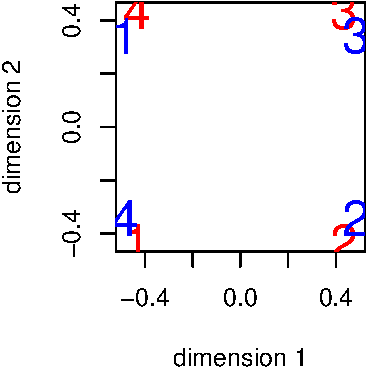
\includegraphics{properties_files/figure-pdf/tmzplot-1.pdf}

}

\caption{Trosset/Mathar Configurations}

\end{figure}%

The two configurations are plotted in figure @ref(fig:tmzplot), with the
global minimizer in red. The non-global configuration (in blue) is
rotated to best least squares fit with the first one, using simple
Procrustus (Gower and Dijksterhuis
(\citeproc{ref-gower_dijksterhuis_04}{2004})). Note that it is a
rectangle, but not a square. The eigenvalues of the Hessian at the
non-global minimum configuration are

\begin{verbatim}
[1] +0.333333 +0.211325 +0.122008 +0.122008 +0.122008 +0.000000 +0.000000
[8] +0.000000
\end{verbatim}

verifying that we indeed have an isolated local minimum. Trosset and
Mathar (\citeproc{ref-trosset_mathar_97}{1997}) verify this using a mix
of symbolic and floating point calculation.

We can generate an additional example using the function equalDelta() in
equaldelta.R. Its arguments are \(n, p, m\), where \(n\) is the order of
the dissimilarity and weight matrices, which have all their non-diagonal
elements equal. Argument \(n\) and \(p\) define the space of
configuration matrices, and \(m\) is the number of smacof runs with a
random start.

\begin{verbatim}
[1] 658
\end{verbatim}

\begin{verbatim}
[1] 342
\end{verbatim}

\begin{verbatim}
itel      1  eiff    0.0000000000  sold    0.0381249159  snew    0.0381249159  
itel      2  eiff    0.0000000000  sold    0.0381249159  snew    0.0381249159  
itel      3  eiff    0.0000000000  sold    0.0381249159  snew    0.0381249159  
itel      4  eiff    0.0000000000  sold    0.0381249159  snew    0.0381249159  
\end{verbatim}

\begin{verbatim}
itel      1  eiff    0.0000000000  sold    0.0357265590  snew    0.0357265590  
itel      2  eiff    0.0000000000  sold    0.0357265590  snew    0.0357265590  
\end{verbatim}

\begin{verbatim}
 [1] +0.200000 +0.129354 +0.129354 +0.102242 +0.102242 +0.079940 +0.079940
 [8] +0.005686 +0.005686 -0.000000 -0.000000 -0.000000
\end{verbatim}

\begin{verbatim}
 [1] +0.200000 +0.114739 +0.114739 +0.107180 +0.073205 +0.073205 +0.051287
 [8] +0.051287 +0.039230 +0.000000 +0.000000 -0.000000
\end{verbatim}

\subsubsection{Directions of Descent}\label{directions-of-descent}

We now go back to the stationary equilateral triangle with center. We
have seen that the gradient at this configuration is zero and the
Hessian is positive semi-definite but rank-deficient. A \emph{descent
direction} at \(X\) is any configuration \(Y\) such that
\(\sigma(X+\epsilon Y)<\sigma(X)\) if \(\epsilon\) is small enough. In
our example, with \(X\) the triangle with center, we must choose \(Y\)
in the null space of the Hessian, because otherwise \(Y\) is a direction
of accent. The null space has two trivial dimensions, \(X\) and \(XA\)
with \(A\) anti-symmetric. The non-trivial null space has dimension
three, and we choose a basis of three orthonormal directions. Then

\[
\sigma(X+\epsilon Y)=\sigma(X)+0+0+\frac16\epsilon^3d^3\sigma(X)(Y,Y,Y)+o(\epsilon^3),
\] and we can find a descent direction if
\(d^3\sigma(X)(Y,Y,Y)\not= 0\).

\begin{verbatim}
[1] +0.066987 -0.000000 +0.000000 -0.186030
\end{verbatim}

\begin{verbatim}
[1] +0.066987 +0.000000 +0.000000 +0.293283
\end{verbatim}

\begin{verbatim}
[1] +0.066987 -0.000000 +0.000000 -0.117607
\end{verbatim}

\bookmarksetup{startatroot}

\chapter{Stress Spaces}\label{propspaces}

Stress is a function of many variables. Consequently there are many
equivalent ways to define it by transforming the parameter space. In
this chapter we discuss the major parametrizations that have actually
been used. Each has its advantages and disadvantages.

\section{Configuration Space}\label{propconfspace}

So far we have defined stress on \(\mathbb{R}^{n\times p}\), the space
of all matrices with \(n\) rows and \(p\) columns. We call this
\emph{configuration space}. The usual MDS representation of a
dissimilarity matrix is a scatterplot of \(n\) points in \(p\)
dimensions. Therefor there is little doubt that configuration space is
the most natural MDS space, and most of our theorems and derivations use
this space.

Nevertheless, configuration space has some disadvantages. Even for \(n\)
as small as four and \(p\) as small as two the dimension of the space of
configurations is eight, and there is no compelling way to visualize
stress as a function of eight variables. Secondly, if we work in
configuration space we have to keep the indeterminacies of the
representation in mind. Because of translational indeterminacy,
minimizing stress over \(X\in\mathbb{R}^{n\times p}\) will give the same
result as minimizing stress over \(X\in\mathbb{R}_C^{n\times p}\), the
\(p(n-1)\)-dimensional subspace of all column-centered matrices. Because
of translational and rotational indeterminacy it will also give the same
result as minimizing stress over \(X\in\mathbb{R}_{CT}^{n\times p}\),
the \(np-\frac12p(p+1)\) dimensional subspace of all centered lower
triangular configurat ions (which have \(x_{ij}=0\) for all \(j>i\)). Or
the same result as minimizing stress over the \(np-\frac12p(p+1)\)
dimensional nonlinear manifold \(\mathbb{R}_{CO}^{n\times p}\) of all
centered orthogonal configurations. Especially rotational indeterminacy
complicates our analysis of MDS algorithms that operate on configuration
space.

Another disadvantage of configuration space is that it needlessly
complicates some of our formulas and derivations. Not all pairs of
coordinate in a configuration \(X\) have the same status. Some pairs
belong to the same row of the matrix, and some pairs to different rows.
Some pairs of coordinates are in the same column, and some are in
different columns. This complicates formulas which depend on considering
pairs of coordinates, such as second derivatives.

One way to make a picture in configuration space is to plot the \(np\)
individual coordinates as functions of a one-dimensional perturbation.
In figure @ref(fig:piccoorc) we illustrate this with an example. We have
four objects, with all weights and dissimilarities equal, and the
\(4\times 2\) configuration is an equilateral triangle together with its
centroid. Everything is suitably scaled, and we perturb each coordinate
using 101 values equally spaced between -1 and +1.

\begin{figure}[H]

{\centering 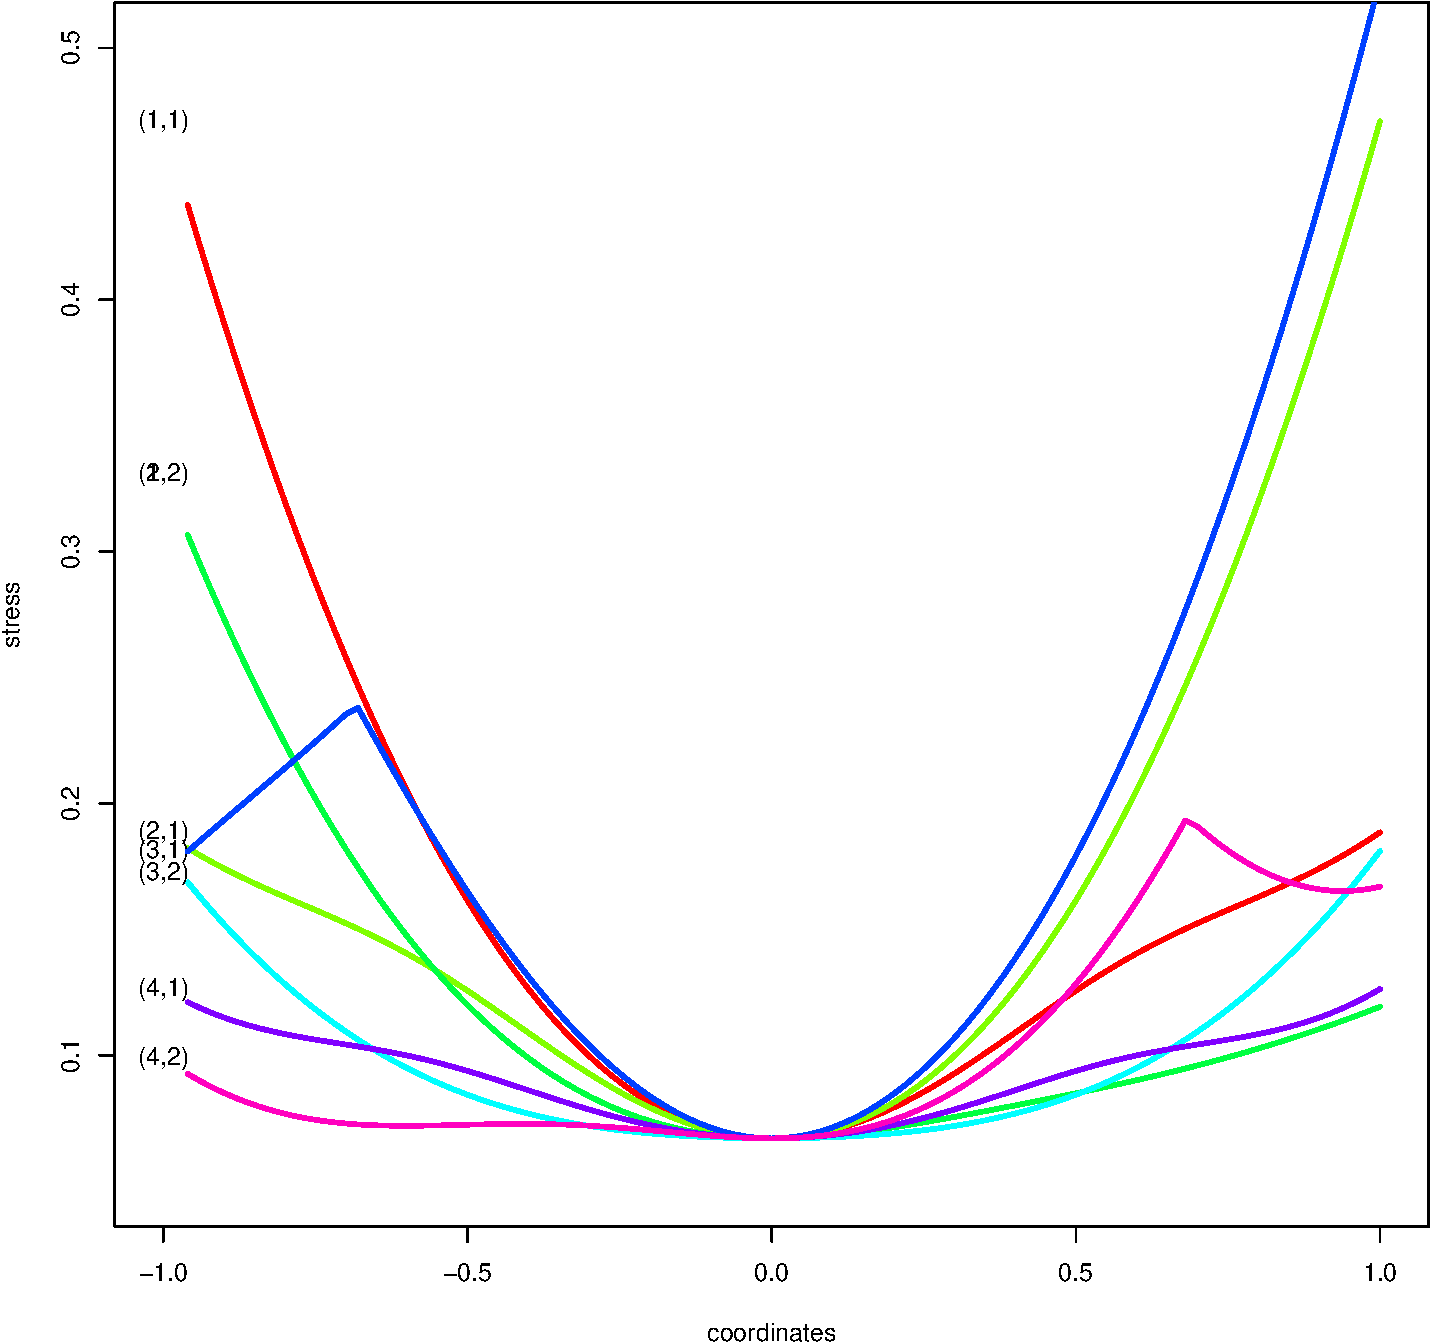
\includegraphics{spaces_files/figure-pdf/piccoorc-1.pdf}

}

\caption{One Coordinate at a Time}

\end{figure}%

\begin{Shaded}
\begin{Highlighting}[]
\NormalTok{delta }\OtherTok{\textless{}{-}} \FunctionTok{wdef}\NormalTok{(}\DecValTok{4}\NormalTok{)}
\NormalTok{w }\OtherTok{\textless{}{-}} \FunctionTok{wdef}\NormalTok{(}\DecValTok{4}\NormalTok{)}
\NormalTok{w }\OtherTok{\textless{}{-}}\NormalTok{ w }\SpecialCharTok{/} \FunctionTok{sum}\NormalTok{(w)}
\NormalTok{s }\OtherTok{\textless{}{-}} \FunctionTok{sum}\NormalTok{ (w }\SpecialCharTok{*}\NormalTok{ delta }\SpecialCharTok{\^{}} \DecValTok{2}\NormalTok{)}
\NormalTok{delta }\OtherTok{\textless{}{-}}\NormalTok{ delta }\SpecialCharTok{/} \FunctionTok{sqrt}\NormalTok{ (s)}
\NormalTok{x }\OtherTok{\textless{}{-}} \FunctionTok{matrix}\NormalTok{(}\FunctionTok{c}\NormalTok{(}\DecValTok{0}\NormalTok{,}\DecValTok{0}\NormalTok{,}\DecValTok{1}\NormalTok{,}\DecValTok{0}\NormalTok{,.}\DecValTok{5}\NormalTok{,}\FunctionTok{sqrt}\NormalTok{(}\DecValTok{3}\NormalTok{)}\SpecialCharTok{/}\DecValTok{2}\NormalTok{),}\DecValTok{3}\NormalTok{,}\DecValTok{2}\NormalTok{,}\AttributeTok{byrow =} \ConstantTok{TRUE}\NormalTok{)}
\NormalTok{x }\OtherTok{\textless{}{-}} \FunctionTok{rbind}\NormalTok{(x, }\FunctionTok{apply}\NormalTok{(x, }\DecValTok{2}\NormalTok{, mean))}
\NormalTok{x }\OtherTok{\textless{}{-}} \FunctionTok{apply}\NormalTok{(x, }\DecValTok{2}\NormalTok{, }\ControlFlowTok{function}\NormalTok{(x) x }\SpecialCharTok{{-}} \FunctionTok{mean}\NormalTok{(x))}
\NormalTok{d }\OtherTok{\textless{}{-}} \FunctionTok{as.matrix}\NormalTok{(}\FunctionTok{dist}\NormalTok{(x))}
\NormalTok{s }\OtherTok{\textless{}{-}} \FunctionTok{sum}\NormalTok{ (w }\SpecialCharTok{*}\NormalTok{ delta }\SpecialCharTok{*}\NormalTok{ d) }\SpecialCharTok{/} \FunctionTok{sum}\NormalTok{ (w }\SpecialCharTok{*}\NormalTok{ d }\SpecialCharTok{*}\NormalTok{ d)}
\NormalTok{x }\OtherTok{\textless{}{-}}\NormalTok{ x }\SpecialCharTok{*}\NormalTok{ s}
\NormalTok{d }\OtherTok{\textless{}{-}}\NormalTok{ d }\SpecialCharTok{*}\NormalTok{ s}
\NormalTok{h }\OtherTok{\textless{}{-}} \FunctionTok{smacofR}\NormalTok{(w,}
\NormalTok{            delta,}
            \AttributeTok{p=}\DecValTok{2}\NormalTok{,}
            \AttributeTok{xold =}\NormalTok{ x,}
            \AttributeTok{eps=}\FloatTok{1e{-}15}\NormalTok{,}
            \AttributeTok{xstop=}\ConstantTok{TRUE}\NormalTok{)}
\end{Highlighting}
\end{Shaded}

\begin{verbatim}
itel      1  eiff    0.0000000000  sold    0.0334936491  snew    0.0334936491  
\end{verbatim}

\begin{Shaded}
\begin{Highlighting}[]
\FunctionTok{print}\NormalTok{(}\FunctionTok{eigen}\NormalTok{(h}\SpecialCharTok{$}\NormalTok{h)}\SpecialCharTok{$}\NormalTok{values)}
\end{Highlighting}
\end{Shaded}

\begin{verbatim}
[1]  3.333333e-01  2.559831e-01  2.559831e-01  2.224907e-16  2.146434e-16
[6]  3.456430e-17 -2.151233e-17 -1.812014e-16
\end{verbatim}

\begin{Shaded}
\begin{Highlighting}[]
\NormalTok{x}\OtherTok{\textless{}{-}}\FunctionTok{matrix}\NormalTok{(}\FunctionTok{c}\NormalTok{(}\DecValTok{0}\NormalTok{,}\DecValTok{2}\NormalTok{,}\DecValTok{1}\NormalTok{,}\DecValTok{1}\NormalTok{,}\DecValTok{0}\NormalTok{,}\DecValTok{0}\NormalTok{,}\FunctionTok{sqrt}\NormalTok{(}\DecValTok{3}\NormalTok{),}\FunctionTok{sqrt}\NormalTok{(}\DecValTok{3}\NormalTok{)}\SpecialCharTok{/}\DecValTok{3}\NormalTok{),}\DecValTok{4}\NormalTok{,}\DecValTok{2}\NormalTok{)}
\NormalTok{z}\OtherTok{\textless{}{-}}\FunctionTok{matrix}\NormalTok{(}\FunctionTok{c}\NormalTok{(}\DecValTok{0}\NormalTok{,}\SpecialCharTok{{-}}\DecValTok{2}\NormalTok{,}\FunctionTok{sqrt}\NormalTok{(}\DecValTok{3}\NormalTok{),}\SpecialCharTok{{-}}\DecValTok{2}\SpecialCharTok{{-}}\FunctionTok{sqrt}\NormalTok{(}\DecValTok{3}\NormalTok{)}\SpecialCharTok{/}\DecValTok{3}\NormalTok{,}\DecValTok{0}\NormalTok{,}\DecValTok{0}\NormalTok{,}\FunctionTok{sqrt}\NormalTok{(}\DecValTok{3}\NormalTok{),}\DecValTok{2}\SpecialCharTok{+}\FunctionTok{sqrt}\NormalTok{(}\DecValTok{3}\NormalTok{)),}\DecValTok{4}\NormalTok{,}\DecValTok{2}\NormalTok{)}
\NormalTok{eps }\OtherTok{\textless{}{-}} \FloatTok{0.00001}
\NormalTok{d }\OtherTok{\textless{}{-}} \FunctionTok{as.matrix}\NormalTok{(}\FunctionTok{dist}\NormalTok{(x }\SpecialCharTok{+}\NormalTok{ eps }\SpecialCharTok{*}\NormalTok{ z))}
\FunctionTok{smacofLossR}\NormalTok{(d, w, delta) }
\end{Highlighting}
\end{Shaded}

\begin{verbatim}
[1] 0.2559831
\end{verbatim}

\subsection{Zero Distance Subspaces}\label{propzerodist}

A \emph{zero-distance subspace} is a subspace of configuration space in
which one or more distances are zero. That a zero distance indeed
defines a subspace follows from the fact that the nonlinear equation
\(d_{ij}(X)=0\) is equivalent to the homogeneous linear equation
\(x_i=x_j\).

The number of zero-distance subspaces is the same as the number of set
partitions of \(n\) objects, which is the Bell number \(B_n\). Bell
numbers are defined by the recursion \begin{equation}
B_{n+1}=\sum_{k=0}^n\binom{n}{k}B_k, 
(\#eq:bellnums)
\end{equation} with \(B_0=1\). The next ten Bell numbers
\(B_1,\cdots,B_{10}\) are 1, 2, 5, 15, 52, 203, 877, 4140, 21147, 11597.
So there are lots of zero-distance subspaces.

The gradient in configuration space for all
\(X\in\mathbb{R}^{n\times p}\) is \[
\nabla\sigma(X)=(V-B(X))X.
\] \[
\nabla\tilde\sigma(\theta)=(\tilde V\theta-\tilde B(\theta)\theta)
\] \[
\frac12\{\nabla\tilde\sigma(\theta)\}_s=\text{tr}\ Y_s'(VX-B(X)X)=\text{tr}\ Y_s'\nabla\sigma(X),
\]

with \(X=\sum_{s=1}^r\theta_sY_s\).

Thus \(\nabla\tilde\sigma(\theta)=0\) if and only if
\(\nabla\sigma(X)\in\mathcal{Y}_\perp\), the subspace of
\(\mathbb{R}^{n\times p}\) orthogonal to \(\mathcal{Y}\). Specifically
\(\nabla\sigma(X)=0\) implies \(\nabla\tilde\sigma(\theta)=0\). If the
\(Y_s\) span all of \(\mathbb{R}^{n\times p}\) then
\(\nabla\tilde\sigma(\theta)=0\) if and only if \(\nabla\sigma(X)=0\).

For the relationship between the minimization problems in coefficient
space and configuration space we also study the relationship between the
two Hessians.

For all \(X\) and \(Z\) in configuration space \[
\frac12\nabla^2\sigma(X)(Z,Z)=\text{tr}\ Z'VZ-\mathop{\sum\sum}_{1\leq i<j\leq n}w_{ij}\frac{\delta_{ij}}{d_{ij}(X)}\left\{\text{tr}\ Z'A_{ij}Z-\frac{\{\text{tr}\ Z'A_{ij}Y\}^2}{d_{ij}^2(X)}\right\}
\]

For any \(\theta\) in coefficient space \[
\frac12\nabla^2\tilde\sigma(\theta)=\tilde V-\mathop{\sum\sum}_{1\leq i<j\leq n}w_{ij}\frac{\delta_{ij}}{d_{ij}(\theta)}\left\{\tilde A_{ij}-\frac{\tilde A_{ij}\theta\theta'\tilde A_{ij}}{d_{ij}^2(\theta)}\right\}
\] and thus

\[
\xi'\nabla^2\tilde\sigma(\theta)\xi=\nabla^2\sigma(X)(Z,Z).
\] where \(Z:=\sum_{s=1}^r\xi_s Y_s\) and
\(X:=\sum_{s=1}^r\theta_s Y_s\).

Thus if \(\theta\) is a local minimum in coefficient space then
\(\nabla^2\sigma(X)\) is positive semi-definite on the subspace
\(\mathcal{Y}\). If \(X\in\mathcal{Y}\) but \(Z\not\in\mathcal{Y}\) it
is perfectly possible that \(\nabla^2\sigma(X)(Z,Z)<0\), and thus \(X\)
can be a saddle point in configuration space. If \(X\in\mathcal{Y}\) is
a local minimum in configuration space, then \(\theta\) is a local
minimum in coefficient space. Of course if \(\mathcal{Y}\) is the whole
space then \(\theta\) is a local minimum in coefficient space if and
only if \(X\) is a local minimum in configuration space.

\begin{multline}
\sigma(X(\theta+\epsilon\xi))=\sigma(X(\theta)+\epsilon\mathcal{D}X(\theta)(\xi)+\frac12\epsilon^2\mathcal{D}^2X(\theta)(\xi,\xi))=\\
\sigma(X(\theta))+\epsilon\mathcal{D}\sigma(X(\theta))\mathcal{D}X(\theta)\xi+\frac12\epsilon^2\{\mathcal{D}\sigma(X(\theta))\mathcal{D}^2X(\theta)(\xi,\xi)+\mathcal{D}\sigma(X(\theta))\mathcal{D}\sigma(X(\theta))\}
\end{multline}

\[
\{\mathcal{D}^2X(\theta)(\xi,\xi)\}_{ip}=\sum\sum\xi_s\xi_t\mathcal{D}_{st}x_{ip}(\theta)=\xi'H_{ip}(\theta)\xi
\] \[
\{\mathcal{D}X(\theta)(\xi)\}_{ip}=\sum\xi_s\mathcal{D}_sx_{ip}(\theta)=G_{ip}(\theta)\xi
\]

\[
\mathcal{D}\sigma(X(\theta))=\{V-B(X(\theta))\}X(\theta)=F(\theta)
\]

\[
\mathcal{D}\sigma(\theta)=\mathcal{D}\sigma(X(\theta))\mathcal{D}X(\theta)
\]

\(\sigma(x_{11}(\theta),\cdots,x_{np}(\theta))\)

\[
\mathcal{D}_s\sigma(\theta)=\sum_{i=1}^n\sum_{s=1}^p\mathcal{D}_{ip}\sigma(X(\theta))\mathcal{D}_sx_{ip}(\theta)
\]

\[
\mathcal{D}_{st}\sigma(\theta)=\sum_{i=1}^n\sum_{s=1}^p
\sum_{j=1}^n\sum_{r=1}^p\mathcal{D}_{is,jr}\sigma(X(\theta))\mathcal{D}_sx_{is}(\theta)\mathcal{D}_tx_{jr}(\theta)
+\sum_{i=1}^n\sum_{s=1}^p\mathcal{D}_{is}\sigma(X(\theta))\mathcal{D}_{st}x_{is}(\theta)
\] Now let \(Y_1,Y_2,\cdots,Y_r\) be linearly independent configurations
in \(\mathbb{R}^{n\times p}\), and consider minimizing stress over all
linear combinations \(X\) of the form \(X=\sum_{s=1}^r \theta_sY_s\).

Each linear combination can be identified with a unique vector
\(\theta\in\mathbb{R}^r\), the coefficients of the linear combination.
Thus we can also formulate our problem as minimizing stress over
\emph{coefficient space}, which is simply \(\mathbb{R}^r\). We write
\(d_{ij}(\theta)\) for \(d_{ij}(X)\) and \(\sigma(\theta)\) for
\(\sigma(X)\). Note that \(d_{ij}(\theta)=\sqrt{\theta'C_{ij}\theta}\),
where \(C_{ij}\) has elements
\(\{C_{ij}\}_{st}:=\text{tr}\ Y_s'A_{ij}Y_t\).

If the \(Y_t\) are actually a basis for configuration space (i.e.~if
\(r=np\)) then minimizing over configuration space and coordinate space
is the same thing. For the \(Y_t\) we could choose all rank one
matrices, for example, of the form \(a_i^{\ }b_s'\) where the \(a_i\)
are a basis for \(\mathbb{R}^n\) and the \(b_s\) are a basis for
\(\mathbb{R}^p\). And, in particular, the \(a_i\) and \(b_s\) can be
chosen as unit vectors of length \(n\) and \(p\), respectively. That
case we have \(C_{ij}=I_p\otimes A_{ij}\), i.e.~the direct sum of \(p\)
copies of \(A_{ij}\). Also if \(\theta=\text{vec}(X)\) then
\(d_{ij}(X)=\sqrt{\theta'(I_p\otimes A_{ij})\theta}\)

If \(r<np\) then coefficient space defines a proper subspace of
configuration space. If it happens to be the \((n -1)p\) dimensional
subspace of all column-centered matrices, then the two approaches still
define the same minimization problem. But in general \(r<(n-1)p\) with
the \(Y_s\) column-centered defines a \emph{constrained MDS problem},
which we analyze in more detail in chapter @ref(cmds).

Coefficient space is also a convenient place to deal with rotational
indeterminacy in basic MDS. It follows from QR decomposition that any
configuration matrix can be rotated in such a way that it upper diagonal
elements (the \(x_{ij}\) with \(i<j\)) are zero (define \(X_p\) to be
the first \(p\) rows of \(X\), compute \(X_p'=QR\) with \(Q\) square
orthonormal and \(R\) upper triangular, thus \(X_p=R'Q'\) and
\(X_pQ=R'\), which is lower triangular). The column-centered upper
triangular configurations are a subspace of dimension
\(p(n-1)-p(p-1)/2\), and we can choose the \(Y_s\) as a basis for this
subspace. In this way we eliminate rotational indeterminacy in a
relatively inexpensive way.

If \(X=\sum_{s=1}^r \theta_sY_s\) then we define the symmetric positive
definite matrix \(B(\theta)\) of order \(r\) with elements

\begin{equation}
b_{st}(\theta):=\text{tr}\ Y_s'B(X)Y_t,
(\#eq:propcoefb)
\end{equation}

where \(B(X)\) is the usual B-matrix of order \(n\) in configuration
space, defined in equation @ref(eq:bdef). Also define \(V\) of order
\(r\) by

\begin{equation}
v_{st}:=\text{tr}\ Y_s'VY_t,
(\#eq:propcoefv)
\end{equation}

where the second \(V\), of order \(n\), is given by equation
@ref(eq:vdef). Then

\begin{equation}
\sigma(\theta)=1-2\ \theta'B(\theta)\theta+\theta'V\theta.
(\#eq:propcoefs)
\end{equation}

The relationship between the stationary points in configuration space
and coefficient space is fairly straightforward.

\phantomsection\label{confcoef}
Suppose \(\theta\) is in coefficient space and
\(X=\sum_{s=1}^r\theta_s Y_s\) is the corresponding point in
configuration space.

\begin{enumerate}
\def\labelenumi{\arabic{enumi}.}
\tightlist
\item
  If \(X\) is a stationary point in configuration space then \(\theta\)
  is a stationary point in coefficient space.
\item
  If \(\theta\) is a stationary point in coefficient space then \(X\) is
  a stationary point in configuration space if and only if
  \(\text{rank}(Y_1\mid\cdots\mid Y_r)\geq n-1\). (THIS IS WRONG)
\end{enumerate}

\begin{proof}
We have \(B(X)X=VX\), i.e.~ \begin{equation}
\sum_{s=1}^r \theta_s B(X)Y_s=\sum_{s=1}^r \theta_s VY_s.
(\#eq:propfitoff)
\end{equation} Premultiplying both sides by \(Y_t'\) and taking the
trace gives \(B(\theta)\theta=V\theta\). This proves the first part.

For the second part, suppose \(B(\theta)\theta=V\theta\) and define
\(X=\sum_{s=1}^r\theta_s Y_s\). Then

\begin{equation}
\sum_{t=1}^r\text{tr}\ Y_s'(B(X)-V)X=0.
(\#eq:propfftofi)
\end{equation}

Thus \(B(X)X=VX\) if and only if \(Y_s'(B(X)-V)X=0\) for all \(s\),
which translates to the rank condition in the theorem (this is WRONG,
correct).
\end{proof}

The advantage of working in coefficient space is that formulas tend to
become more simple. Functions are defined on \(\mathbb{R}^r\), and not a
space of matrices, in which some coordinates belong to the same point
(row) and others to other points (rows), and some are on the same
dimension (column), while others are on different dimensions (columns).

Note that expressions such as @ref(eq:propfitoff) and
@ref(eq:propfitoff) simplify if the \(Y_s\) are \(V\)-orthonormal,
i.e.~if \(\text{tr}\ Y_s'VY_t=\delta^{st}\) and thus \(V=I\). It is easy
to generate such an orthonormal set from the original \(Y_s\) by using
the Gram-Schmidt process. The R function gramy() in utilities.R does
exactly that. Coefficient space, which is the span of the \(Y_s\), is
not changed by the orthogonalization process.

For a \(V\)-orthonormal set \(Y\) we have the stationary equations
\(B(\theta)\theta=\theta\), which says that \(\theta\) is an eigenvector
of \(B(\theta)\) with eigenvalue 1.

The Hessian is

\begin{equation}
\mathcal{D}^2\sigma(\theta)=I-H(\theta),
(\#eq:hessmat)
\end{equation}

with

\begin{equation}
H(\theta):=\mathcal{D}^2\rho(\theta)=\mathop{\sum\sum}_{1\leq i<j\leq n}w_{ij}\frac{\delta_{ij}}{d_{ij}(\theta)}\left\{C_{ij}-\frac{C_{ij}\theta\theta'C_{ij}}{\theta'C_{ij}\theta}\right\}.
(\#eq:rhohessdef)
\end{equation}

We have \(0\lesssim H(\theta)\lesssim B(\theta)\) and thus
\(I-B(\theta)\lesssim\mathcal{D}^2\sigma(\theta)\lesssim I\).

Hessian in coef and conf space

\section{Spherical Space}\label{propspherespace}

\begin{equation}
\min_X\sigma(X)=\min_{\lambda\geq 0}\min_{\eta^2(X)=1}\sigma(\lambda X)=\min_{\eta^2(X)=1}\min_{\lambda\geq 0}\sigma(\lambda X)=
\min_{\eta^2(X)=1}1-\rho^2(X).
(\#eq:homequ)
\end{equation}

We see that basic MDS can also be formulated as maximization of \(\rho\)
over the ellipsoid \(\{X\mid \eta^2(X)=1\}\) or, equivalently, over the
convex ellipsoidal disk \(\{X\mid \eta^2(X)\leq 1\}\). A similar
formulation is available in coefficient space.

This shows that the MDS problem can be seen as a rather special
nonlinear eigenvalue problem. Guttman (\citeproc{ref-guttman_68}{1968})
also discusses the similarities of MDS and eigenvalue problems, in
particular as they relate to the power method. In linear eigenvalue
problems we maximize a convex quadratic form, in the MDS problem we
maximize the homogeneous convex function \(\rho\), in both cases over an
ellipsoidal disk. The sublevel sets of \(\rho\) defined as
\(\mathcal{L}_r:=\{X\mid \rho(X)\leq r\}\) are nested convex sets
containing the origin. The largest of these sublevel sets that still
intersects the ellipsoid \(\eta^2(X)=1\) corresponds to the global
minimum of stress.

In two and maybe three dimensions graphical method.

\(\alpha X+\beta Y\) in sphere space one-dimensional

\section{Distance Space}\label{distance-space}

\[
\sigma(D)=\min_{D\in\mathbb{D}}\mathop{\sum\sum}_{1\leq i<j\leq n} w_{ij}(\delta_{ij}-d_{ij})^2.
\] \(\mathbb{D}\) is the set of \(p\)-dimensional Euclidean distance
matrices, which is not convex.

\(\mathbb{D}\) is the set of Euclidean distance matrices, which is not
convex.

If \(D_1\times D_2=0\) then they span a convex cone.

\[
\tau(\alpha D_1+(1-\alpha)D_2)^{(2)})=\alpha^2 \tau(D_1^2)+(1-\alpha)^2\tau(D_2^2)+2\alpha(1-\alpha)\tau(D_1\times D_2)
\] So if \(\tau(D_1\times D_2)\gtrsim 0\) convex.

\(\mathbb{D}\) is the set of distance matrices, which is convex.

Distance matrices are defined by linear inequalities.

\(\mathbb{D}\) is the set of ultrametric matrices,
\(d_{ij}\leq\max(d_{ik},d_{jk})\), which is not convex.

If \(D\in\mathbb{D}\) then \(\sqrt{D}\in\mathbb{D}\)

\section{Squared Distance Space}\label{squared-distance-space}

\[
\min_{D\in\mathbb{E}}\mathop{\sum\sum}_{1\leq i<j\leq n}w_{ij}(\delta_{ij}-d_{ij})^2.
\] \(\mathbb{E}\) is the set of squared Euclidean distance matrices,
which is convex.

If \(E\in\mathbb{E}\) then \(\sqrt{E}\in\mathbb{D}\)

\section{Gramian Space}\label{gramian-space}

We can write \(d_{ij}^2(X)=\text{tr}\ X'A_{ij}X = \text{tr}\ A_{ij}C,\)
with \(C=XX'\). This shows minimizing stress can also be formulated as
minimizing

\begin{equation}
\sigma(C)=1+\text{tr}\ VC-2\mathop{\sum\sum}_{1\leq i<j\leq n}w_{ij}\delta_{ij}\sqrt{\text{tr}\ A_{ij}C}
(\#eq:stresspsd)
\end{equation}

over all \(C\gtrsim 0\) of rank \(r\leq p\).

\section{Pictures of Stress}\label{picsstress}

Even for \(n\) as small as four and \(p\) as small as two the dimension
of the space of centered configurations is six, and there is no natural
way to visualize a function of six variables. What we can do is plot
stress on two-dimensional subspaces, either as a contour plot or as a
perspective plot. Our two-dimensional subspaces are of the form
\(\alpha X+\beta Y\), where \(X\) and \(Y\) are fixed configurations.
Much of this chapter is a modified, and in some places expanded, version
of De Leeuw (\citeproc{ref-deleeuw_E_16l}{2016c}).

Throughout we use a small example of order \(n=4\) which all
dissimilarities equal. The same example has been analyzed by De Leeuw
(\citeproc{ref-deleeuw_A_88b}{1988}), De Leeuw
(\citeproc{ref-deleeuw_R_93c}{1993}), Trosset and Mathar
(\citeproc{ref-trosset_mathar_97}{1997}), and Zilinskas and Poslipskyte
(\citeproc{ref-zilinskas_podlipskyte_03}{2003}). For this example a
global minimum in two dimensions has its four points in the corners of a
square. That is our \(X\), which has stress 0.0285955. Our \(Y\) is
another stationary point, which has three points in the corners of an
equilateral triangle and the fourth point in the center of the triangle.
Its stress is 0.0669873. We column-center the configurations and scale
them so that they are actually stationary points, i.e.~so that
\(\eta^2(X)=\rho(X)\) and \(\eta^2(Y)=\rho(Y)\). The example is chosen
in such a way that there are non-zero \(\alpha\) and \(\beta\) such that
\(d_{12}(\alpha X+\beta Y)=0\). In fact \(d_{12}\) is the only distance
that can be made zero by a non-trivial linear combination.

Another way of looking at the two configurations is that \(X\) are four
points equally spaced on a circle, and \(Y\) are three points equally
spaced on a circle with the fourth point in the center of the circle. De
Leeuw (\citeproc{ref-deleeuw_A_88b}{1988}) erroneously claims that \(Y\)
is a non-isolated local minimum of stress, but Trosset and Mathar
(\citeproc{ref-trosset_mathar_97}{1997}) have shown there exists a
descent direction at \(Y\), and thus \(Y\) is actually a saddle point.
Of course the stationary points defined by \(X\) and \(Y\) are far from
unique, because we can permute the four points over the corners of the
square and the triangle in many ways.

\subsection{Coefficient Space}\label{coefficient-space}

Configurations as a linear combination of a number of given
configurations have already been discussed in general in chapter
@ref(propchapter), section @ref(propspaces) as the transformation from
configuration space to coefficient space. Since we are dealing here with
the special case of linear combinations of only two configurations we
specialize some of these general results.

We start with \(d_{ij}^(\theta)=\theta'T_{ij}\theta\), where \(\theta\)
has elements \(\alpha\) and \(\beta\), and where \(T\) is the
\(2\times 2\) matrix with elements \begin{equation}
t_{ij}:=\begin{bmatrix}
\text{tr}\ X'A_{ij}X&\text{tr}\ X'A_{ij}Y\\
\text{tr}\ Y'A_{ij}X&\text{tr}\ Y'A_{ij}Y
\end{bmatrix}
(\#eq:pictbform)
\end{equation}

Then

\begin{equation}
\tilde\sigma(\theta):=1-2\ \theta'C(\theta)\theta+\theta'U\theta,
(\#eq:picstress2)
\end{equation}

where, using \(Z(\theta)=\alpha X+\beta Y\),

\begin{equation}
C(\theta):=
\begin{bmatrix}
\text{tr}\ X'B(Z(\theta))X&\text{tr}\ X'B(Z(\theta))Y\\
\text{tr}\ Y'B(Z(\theta))X&\text{tr}\ Y'B(Z(\theta))Y
\end{bmatrix},
(\#eq:pictbformc)
\end{equation}

and

\begin{equation}
U:=\begin{bmatrix}
\text{tr}\ X'VX&\text{tr}\ X'VY\\
\text{tr}\ Y'VX&\text{tr}\ Y'VY
\end{bmatrix}.
(\#eq:pictbformu)
\end{equation}

We have used \(\tilde\sigma\) in equation @ref(eq:picstress2) to
distinguish stress on the two-dimensional space of coefficients from
stress on the eight-dimensional space of \(4\times 2\) configurations.
Thus \(\tilde\sigma(\alpha,\beta)=\sigma(\alpha X + \beta Z)\).

The gradient at \(\theta\) is

\begin{equation}
\nabla\tilde\sigma(\theta)=U\theta-C(\theta)\theta,
(\#eq:picgrad2)
\end{equation}

and the Hessian is

\begin{equation}
\nabla^2\tilde\sigma(\theta)=U-\mathop{\sum\sum}_{1\leq i<j\leq n}
w_{ij}\frac{\delta_{ij}}{d_{ij}(\theta)}\left\{T_{ij}-\frac{T_{ij}\theta\theta'T_{ij}}{\theta'T_{ij}\theta}\right\}.
(\#eq:pichess2)
\end{equation}

\begin{center}\rule{0.5\linewidth}{0.5pt}\end{center}

\phantomsection\label{pictpreserve}
If \(B(X)X=VX\) and \(\theta=\begin{bmatrix}1&0\end{bmatrix}\) then
\(C(\theta)\theta=U\theta\).

\begin{center}\rule{0.5\linewidth}{0.5pt}\end{center}

\begin{proof}
If \(B(X)X=VX\) and \(\theta=\begin{bmatrix}1&0\end{bmatrix}\) then, by
equations @ref(eq:pictbformc) and @ref(eq:pictbformu),

\begin{equation}
U-C(\theta)=\begin{bmatrix}0&0\\0&\text{tr}\ Y'(V-B(X))Y\end{bmatrix}.
(\#eq:picuminc)
\end{equation}

Thus \((U-C(\theta))\theta=0\).
\end{proof}

\begin{center}\rule{0.5\linewidth}{0.5pt}\end{center}

Thus each stationary point of \(\sigma\) gives a stationary point of
\(\tilde\sigma\). The other way around, however, we are not so lucky.

\begin{center}\rule{0.5\linewidth}{0.5pt}\end{center}

\phantomsection\label{pictaround}
If \(C(\theta)\theta=U\theta\) and if the \(n\times 2p\) matrix
\(\begin{bmatrix}X&Y\end{bmatrix}\) has rank \(n-1\) then \(B(Z)Z=VZ\).

\begin{center}\rule{0.5\linewidth}{0.5pt}\end{center}

\begin{proof}
If \(C(\theta)\theta=U\theta\) then both \(\text{tr}\ X'(V-B(Z)Z)=0\)
and \(\text{tr}\ Y'(V-B(Z))Z=0\). If the \(n\times 2p\) matrix
\(\begin{bmatrix}X&Y\end{bmatrix}\) has rank \(n-1\) then this implies
\((V-B(Z))Z=0\).
\end{proof}

\begin{center}\rule{0.5\linewidth}{0.5pt}\end{center}

In our example the singular values of
\(\begin{bmatrix}X&Y\end{bmatrix}\) are 0.4879059, 0.4333287, 0.2242285,
\ensuremath{2.256597\times 10^{-17}} and thus there is a one-one
correspondence between stationary points of \(\sigma\) and
\(\tilde\sigma\).

\begin{center}\rule{0.5\linewidth}{0.5pt}\end{center}

\phantomsection\label{picsecder}
If \(B(X)X=VX\) and \(\theta=\begin{bmatrix}1&0\end{bmatrix}\) then

\begin{enumerate}
\def\labelenumi{\arabic{enumi}.}
\tightlist
\item
  If \(\text{tr}\ Y'(V-B(X))Y > 0\) then \(\sigma\) has a local minimum
  at theta.
\item
  If \(\sigma\) has a saddle point at \(\theta\) then
  \(\text{tr}\ Y'(V-B(X))Y < 0\).
\end{enumerate}

\begin{center}\rule{0.5\linewidth}{0.5pt}\end{center}

\begin{proof}
Suppose \(B(X)X=VX\) and \(\theta=\begin{bmatrix}1&0\end{bmatrix}\).
Then, from @ref(eq:pichess2) and @ref(eq:picuminc), \[
\nabla^2\sigma(\theta)=\begin{bmatrix}0&0\\0&\text{tr}\ Y'(V-B(X))Y\end{bmatrix}+\mathop{\sum\sum}_{1\leq i<j\leq n}
w_{ij}\frac{\delta_{ij}}{d_{ij}(\theta)}\frac{T_{ij}\theta\theta'T_{ij}}{\theta'T_{ij}\theta}.
\]
\end{proof}

\begin{center}\rule{0.5\linewidth}{0.5pt}\end{center}

In our example \(\text{tr}\ X'(V-B(Y))X\) is -0.1502768 and
\(\text{tr}\ Y'(V-B(X))Y\) is -0.0533599.

\subsection{Global Perspective}\label{global-perspective}

We first make a global perspective plot, over the range \((-2.5,+2.5)\).

\begin{figure}[H]

{\centering 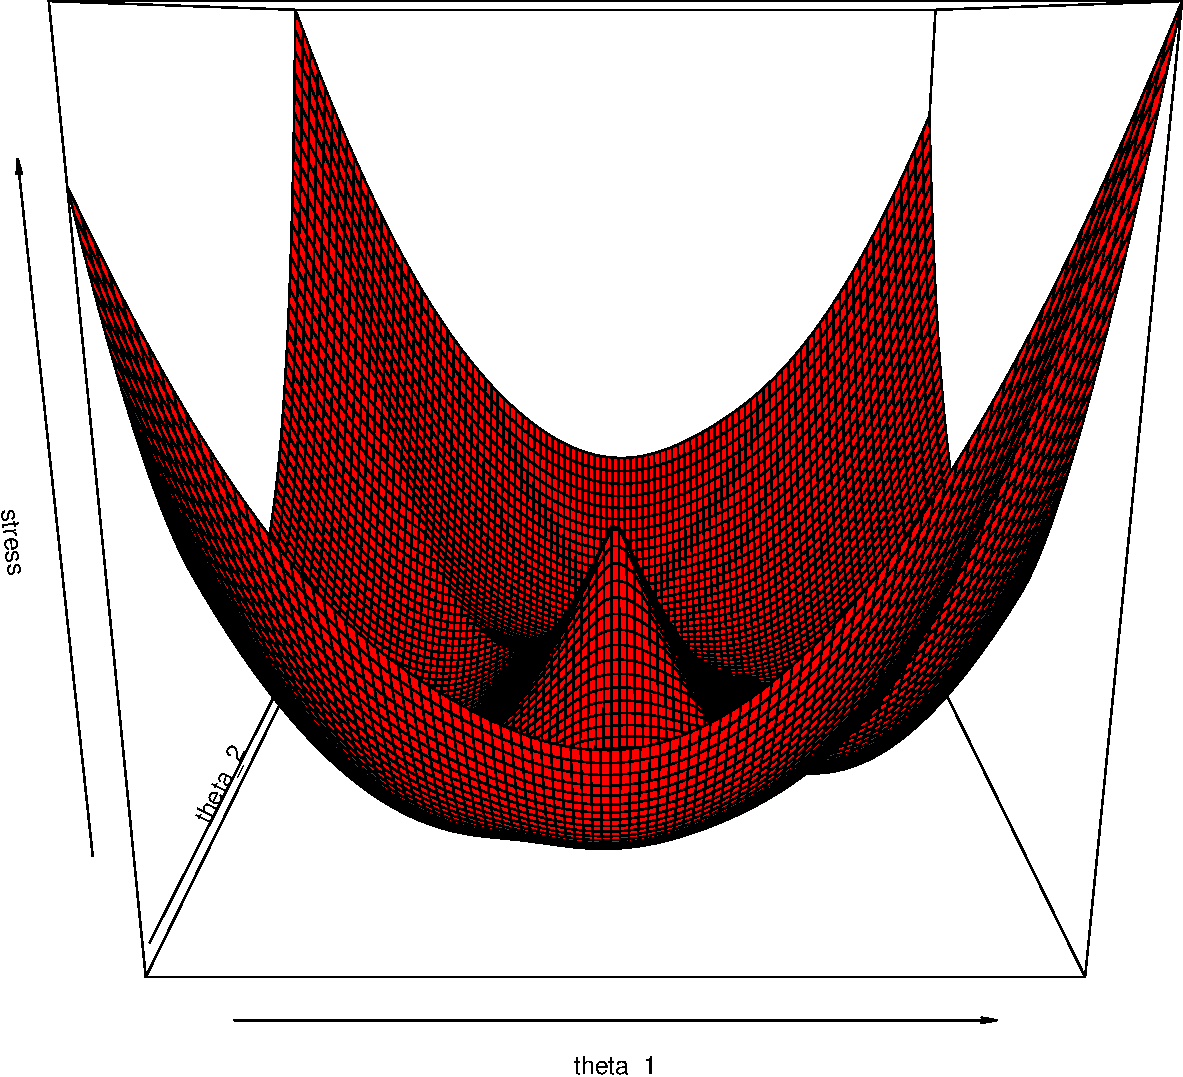
\includegraphics{spaces_files/figure-pdf/globalperspective-1.pdf}

}

\caption{Global Perspective}

\end{figure}%

We see the symmetry, following from the fact that stress is even. We
also see the local maximum at the origin, where stress is not
differentiable. Also note the ridge, where \(d_{12}(\theta)=0\) and
where stress is not differentiable either. The ridge shows nicely that
on rays emanating from the origin stress is a convex quadratic. Also,
far away from the origin, stress globally behaves very much like a
convex quadratic (except for the ridge). Clearly local minima must be
found in the valleys surrounding the small mountain at the origin, all
within the sphere with radius \(\sqrt{2}\).

\subsection{Global Contour}\label{global-contour}

Figure @ref(fig:globalperspective) is a contour plot of stress over
\((-2,+2)\otimes(-2,+2)\). The red line is
\(\{\theta\mid d_{12}(\theta) = 0\}\). The blue line has the minimum of
the convex quadratic on each of the rays through the origin. Thus all
local minima, and in fact all stationary points, are on the blue line.
Note that the plot uses \(\theta\) to define the coordinate axes, not
\(\gamma=(\alpha,\beta)\). Thus there are no stationary points at
\((0,1)\) and \((1,0)\), but at the corresponding points (1.3938469, 0)
and (1.0406404, 0.8849253) in the \(\theta\) coordinates (and, of
course, at their mirror images).

Besides the single local maximum at the origin, it turns out that in
this example there are five pairs of stationary points. Or, more
precisely, I have not been able to find more than five. Each stationary
point \(\theta\) has a mirror image \(-\theta\). Three of the five are
local minima, two are saddle points. Local minima are plotted as blue
points, saddle points as red points.

\begin{figure}[H]

{\centering 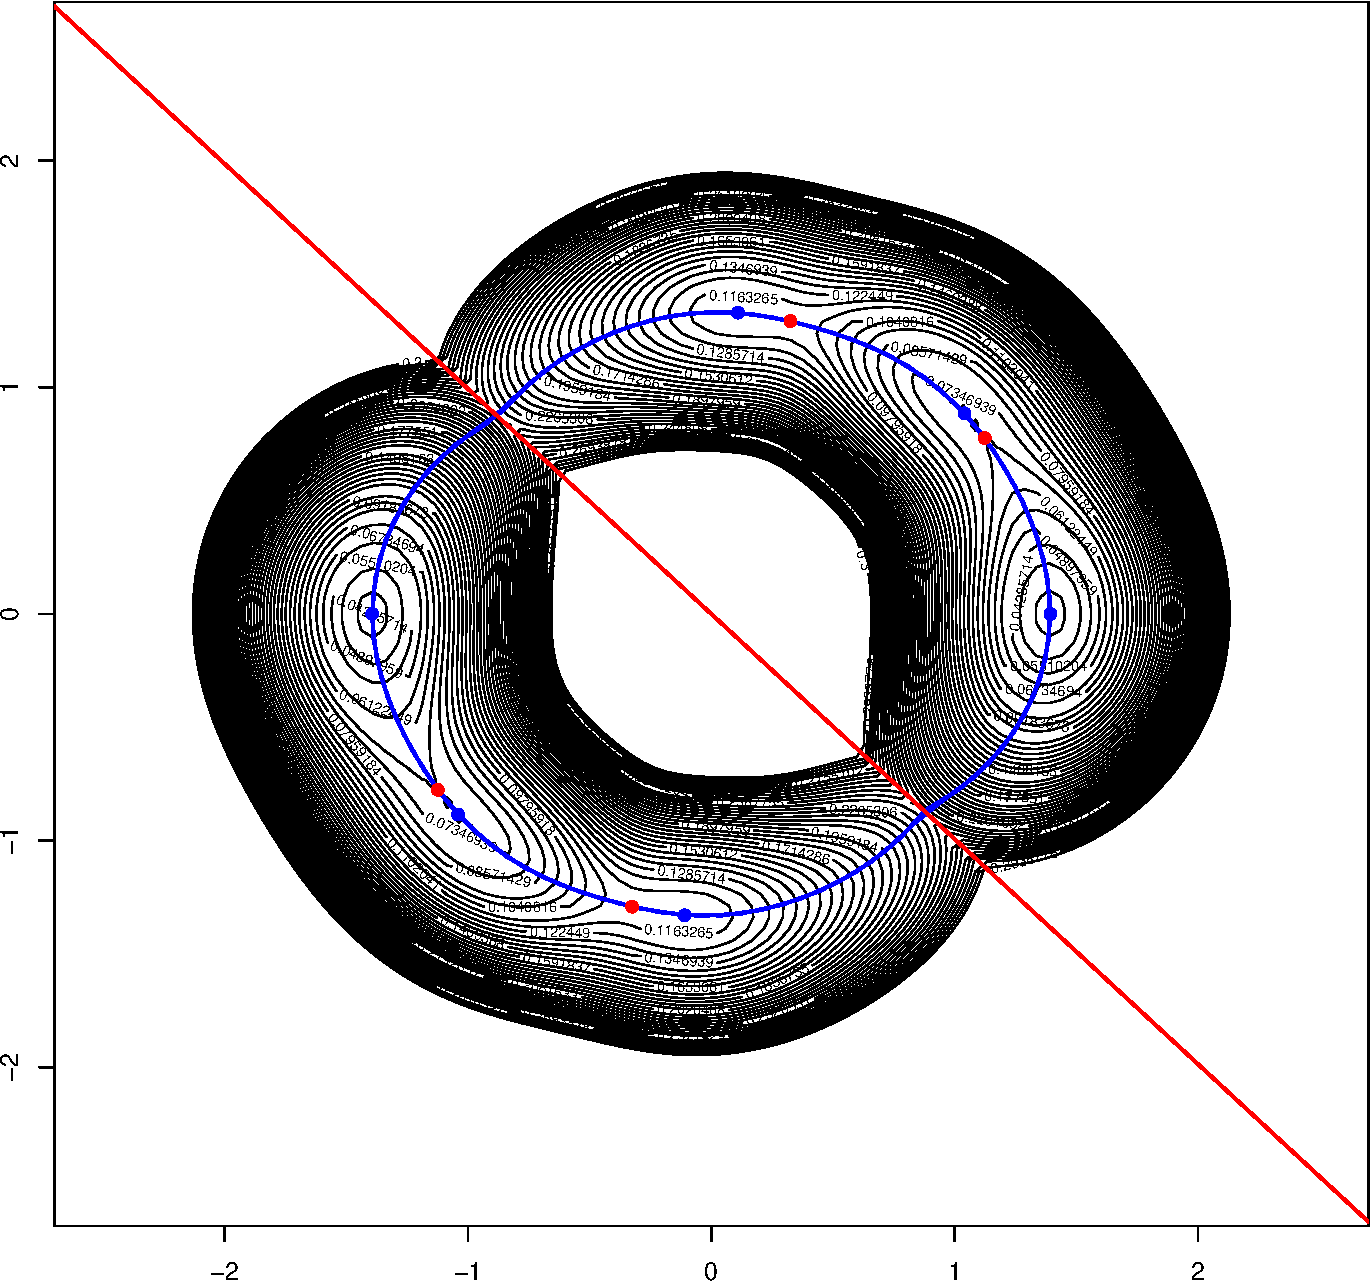
\includegraphics{spaces_files/figure-pdf/globalcontour-1.pdf}

}

\caption{Global Contour}

\end{figure}%

\subsection{Stationary Points}\label{stationary-points}

\subsubsection{First Minimum}\label{first-minimum}

We zoom in on the first local minimum at (1.0406404, 0.8849253). Its
stress is 0.0669873, and the corresponding configuration has three
points in the corners of an equilateral triangle and the fourth point in
its centroid. Note that this local minimum is a saddle point in
configuration space \(\mathbb{R}^{4\times 2}\) (Trosset and Mathar
(\citeproc{ref-trosset_mathar_97}{1997})). The eigenvalues of
\(B(\theta)\) are (1.3686346, 1) and those of the Hessian
\(I-H(\theta)\) are (1, 0.0817218). The area of the contour plot around
the stationary value is in figure @ref(fig:contfirstmin).

\begin{figure}[H]

{\centering 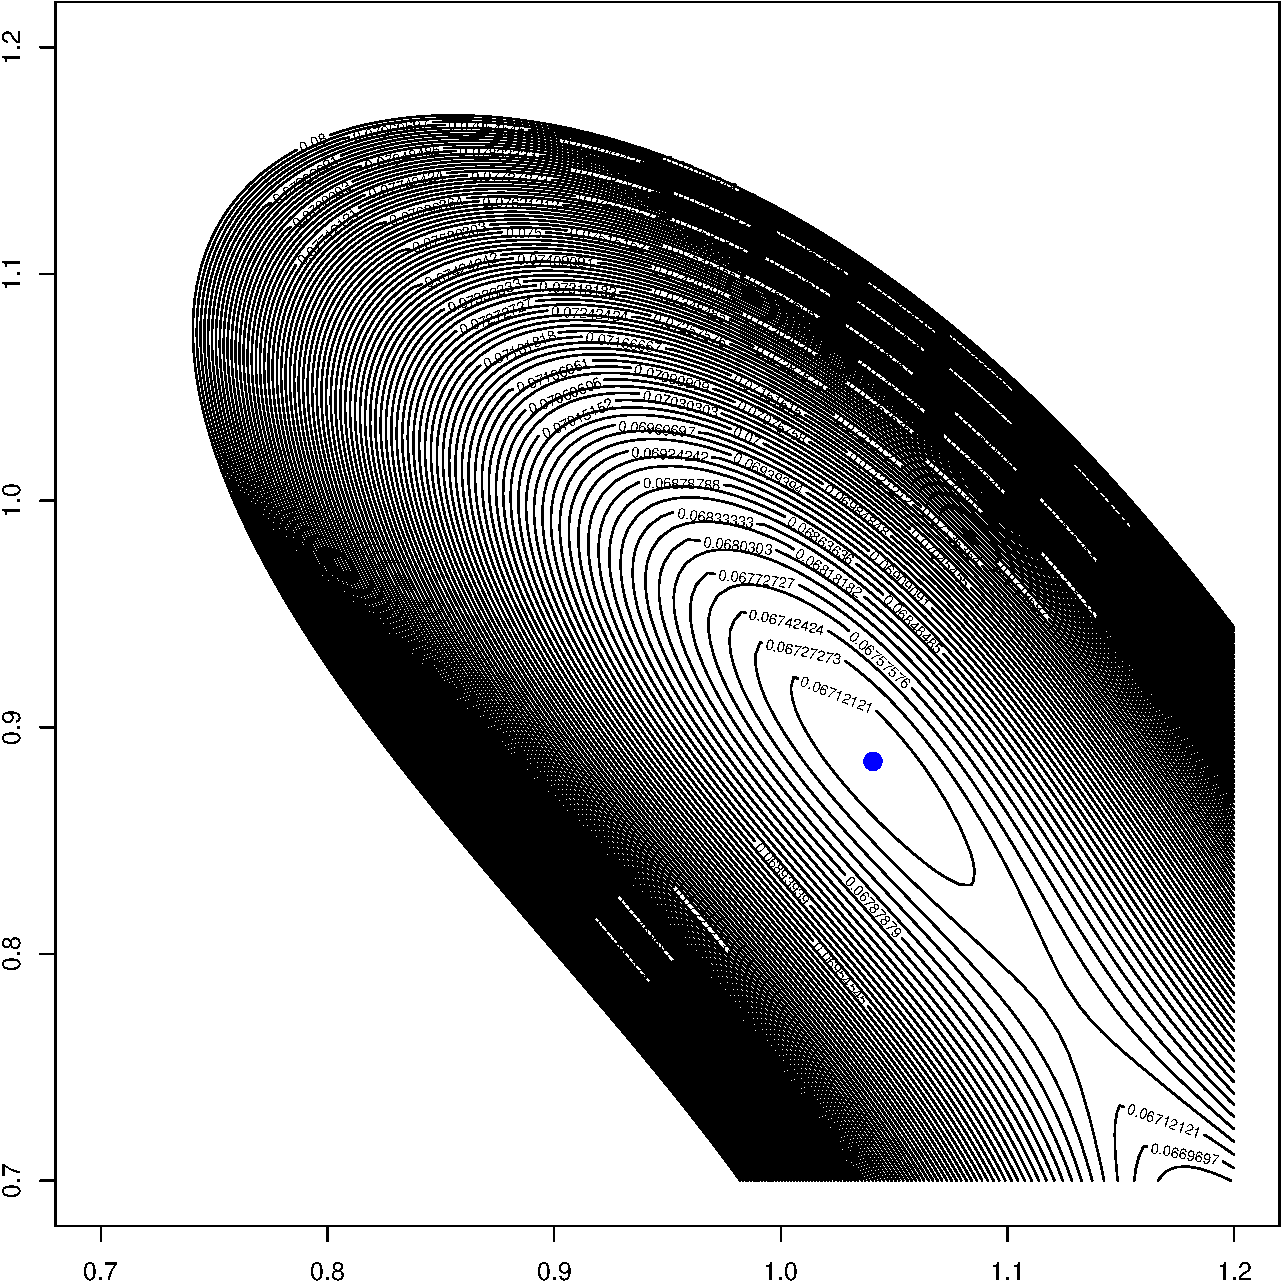
\includegraphics{spaces_files/figure-pdf/contfirstmin-1.pdf}

}

\caption{Contour Plot First Minimum}

\end{figure}%

\subsection{Second Minimum}\label{second-minimum}

The second local minimum (which is the global minimum) at (1.3938469, 0)
has stress 0.0285955. The configuration are the four points at the
corners of a square. The eigenvalues of \(B(\theta)\) are (1.1362799, 1)
and those of the Hessian \(I-H(\theta)\) are (1, 0.3743105). The area of
the contour plot around the stationary value is in figure
@ref(fig:contsecmin).

\begin{figure}[H]

{\centering 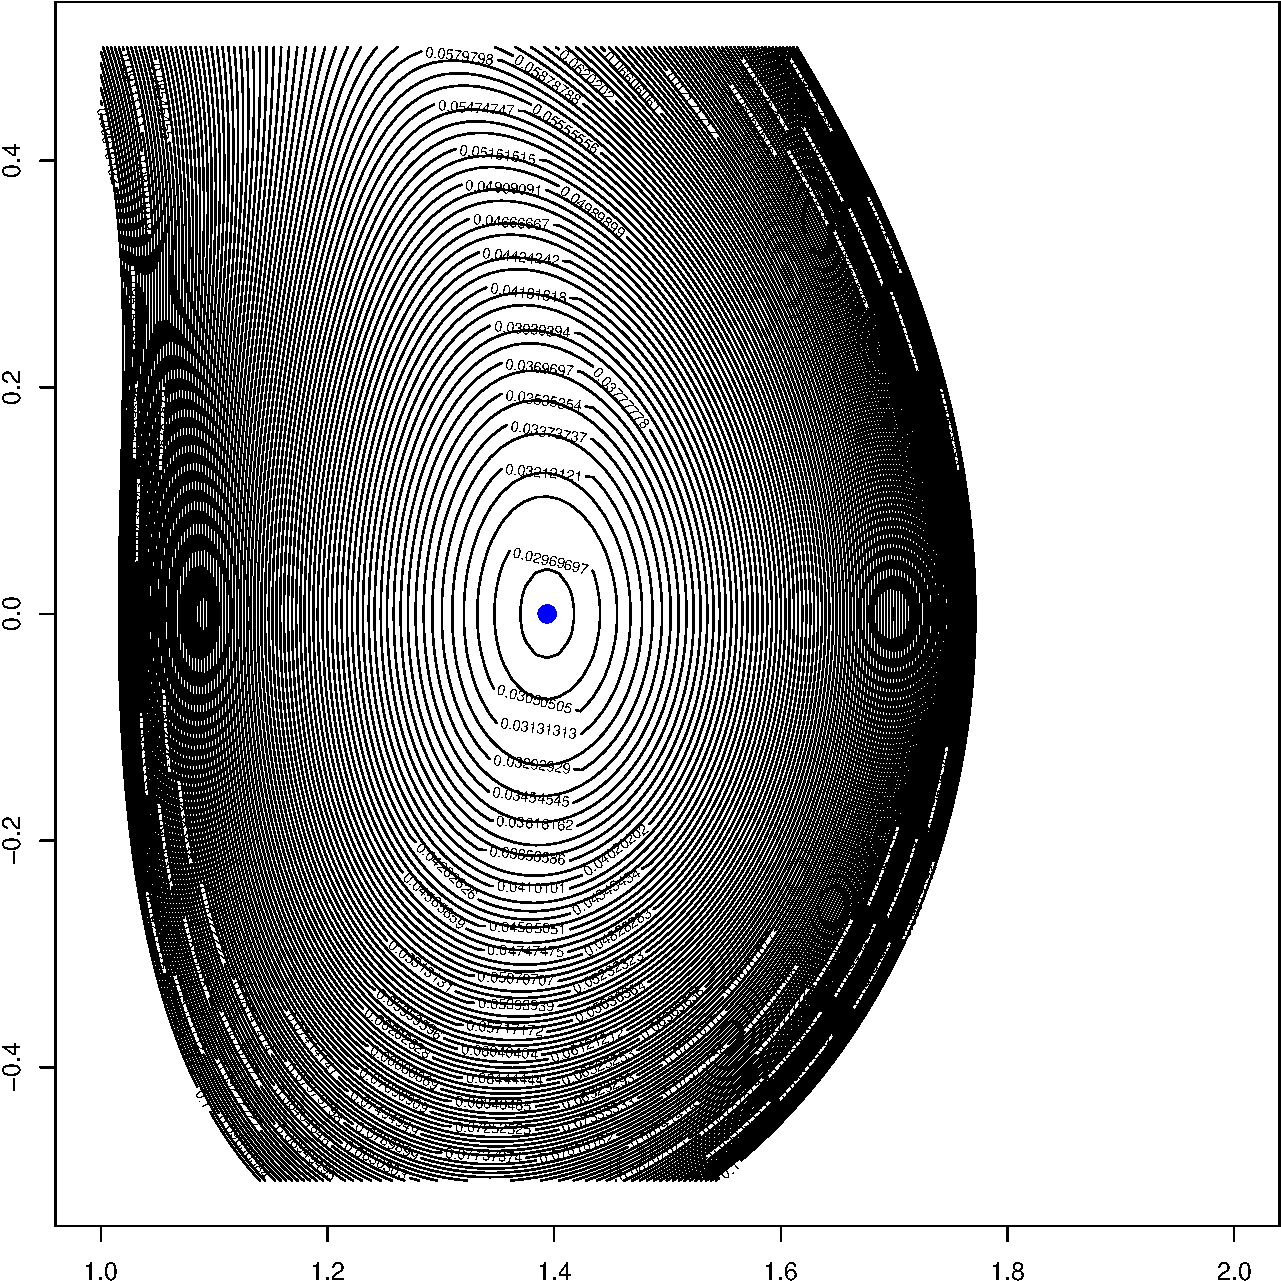
\includegraphics{spaces_files/figure-pdf/contsecmin-1.pdf}

}

\caption{Contour Plot Second Minimum}

\end{figure}%

\subsection{Third Minimum}\label{third-minimum}

The third local minimum at (0.1096253, 1.3291942) has stress 0.1106125,
and the corresponding configuration is in figure @ref(fig:confthirdmin).

\begin{figure}[H]

{\centering 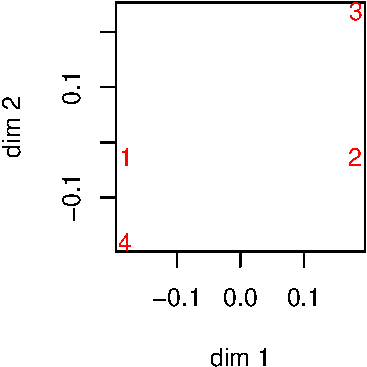
\includegraphics{spaces_files/figure-pdf/confthirdmin-1.pdf}

}

\caption{Configuration Third Minimum}

\end{figure}%

The eigenvalues of \(B(\theta)\) are (1.5279386, 1) and those of the
Hessian \(I-H(\theta)\) are (1, 0.2362079). The area of the contour plot
around the stationary value is in figure @ref(fig:contthirdmin)

\begin{figure}[H]

{\centering 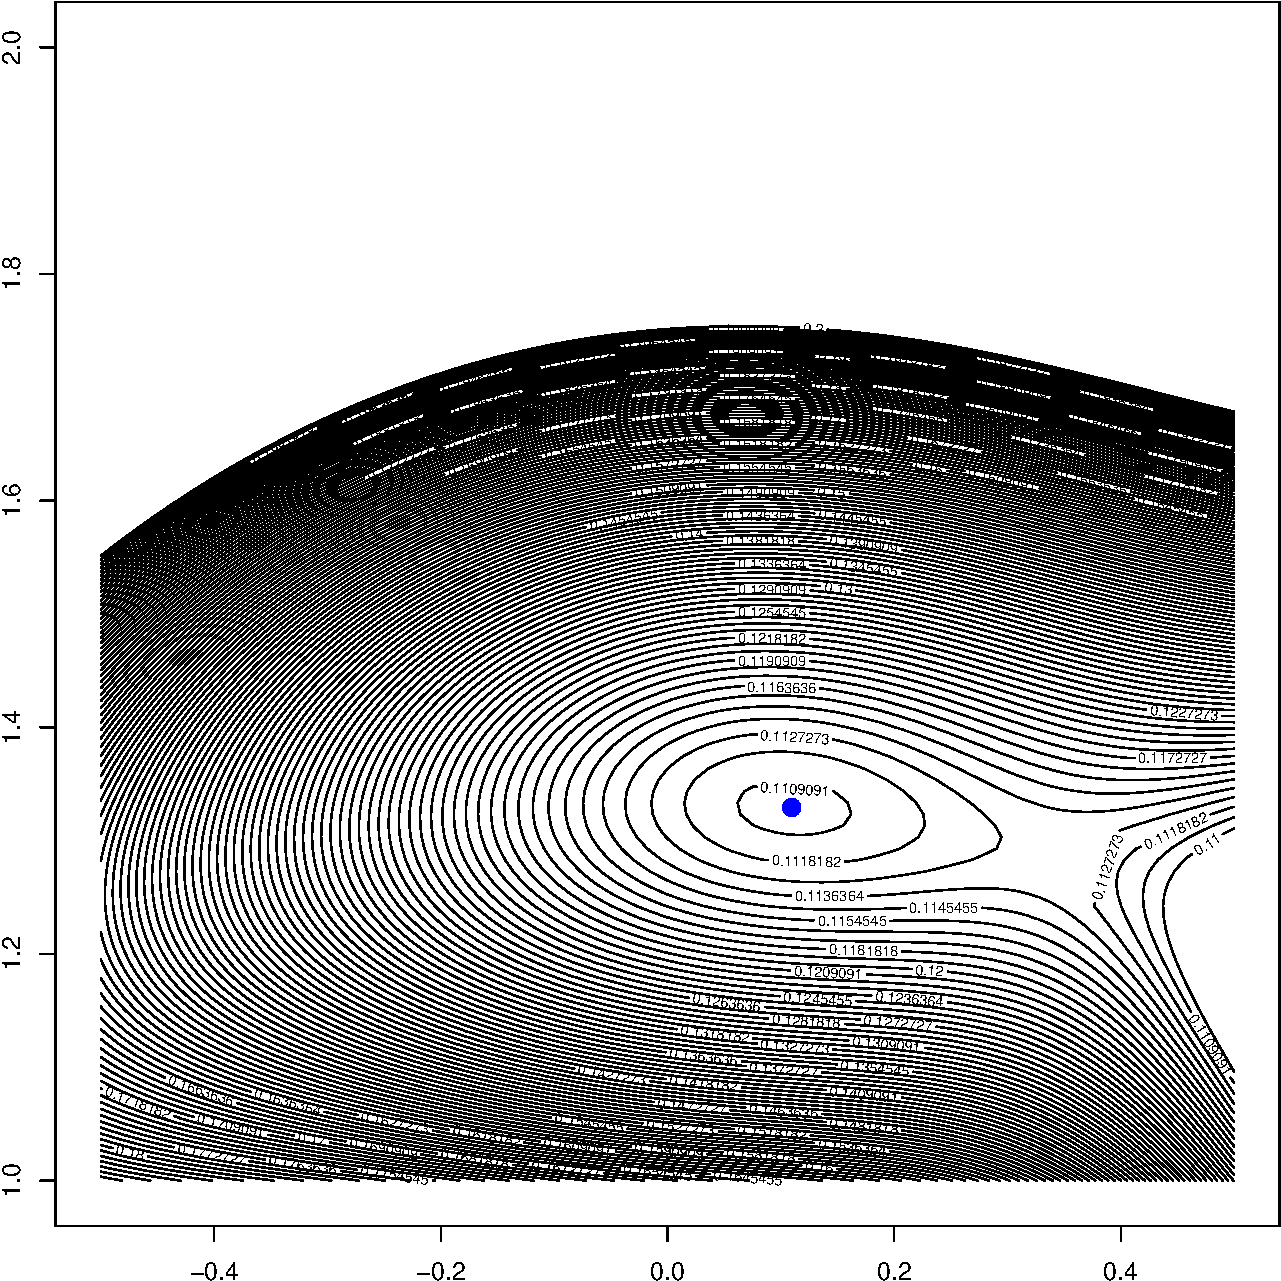
\includegraphics{spaces_files/figure-pdf/contthirdmin-1.pdf}

}

\caption{Contour Plot Third Minimum}

\end{figure}%

\subsection{First Saddle Point}\label{first-saddle-point}

The saddle point at (0.3253284, 1.2916758) has stress 0.1128675, and the
corresponding configuration is in figure @ref(fig:conffirstsad).

\begin{figure}[H]

{\centering 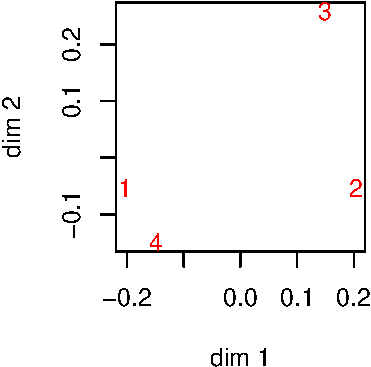
\includegraphics{spaces_files/figure-pdf/conffirstsad-1.pdf}

}

\caption{Configuration First Saddlepoint}

\end{figure}%

The eigenvalues of \(B(\theta)\) are (1.7778549, 1) and those of the
Hessian \(I-H(\theta)\) are (1, -0.311088). The area of the contour plot
around the stationary value is in figure @ref(fig:contfirstsad)

\begin{figure}[H]

{\centering 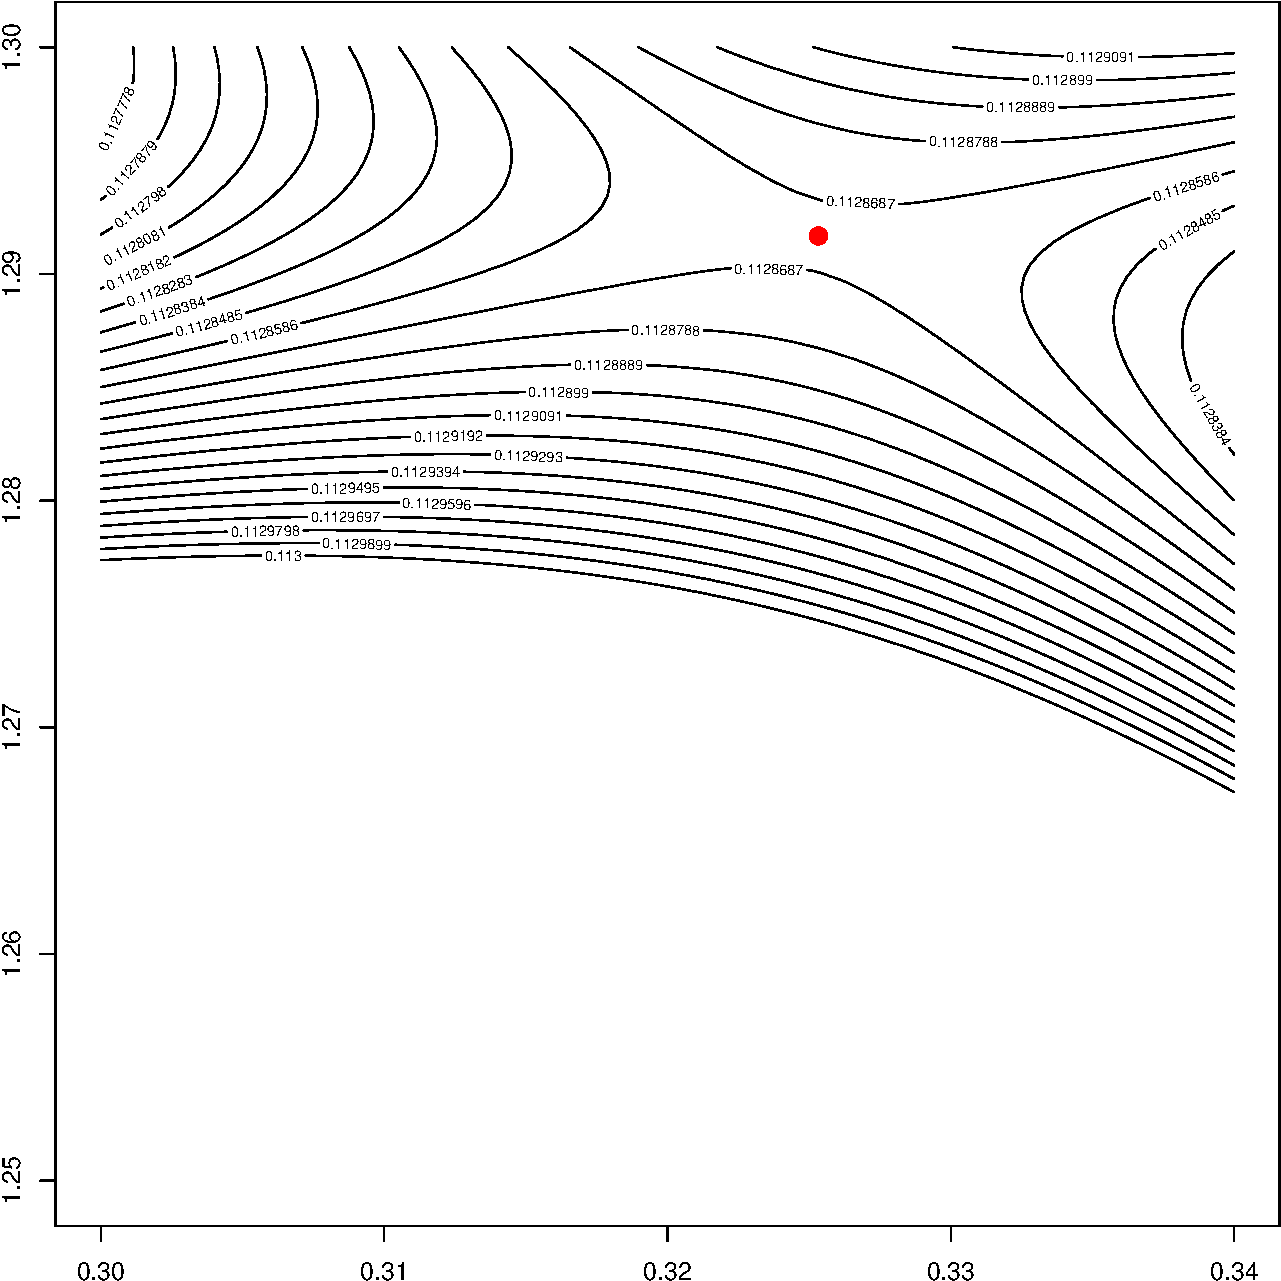
\includegraphics{spaces_files/figure-pdf/contfirstsad-1.pdf}

}

\caption{Contour First Saddlepoint}

\end{figure}%

\subsection{Second Saddle Point}\label{second-saddle-point}

The saddle point at (1.1238371, 0.7762046) has stress 0.0672483 and the
corresponding configuration is in figure @ref(fig:confsecsad)

\begin{figure}[H]

{\centering 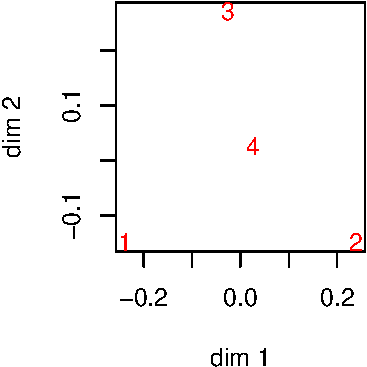
\includegraphics{spaces_files/figure-pdf/confsecsad-1.pdf}

}

\caption{Configuration Second Saddlepoint}

\end{figure}%

The eigenvalues of \(B(\theta)\) are (1.4111962, 1) and those of the
Hessian \(I-H(\theta)\) are (1, -0.0841169). The area of the contour
plot around the stationary value is in figure @ref(fig:contsecsad)

\begin{figure}[H]

{\centering 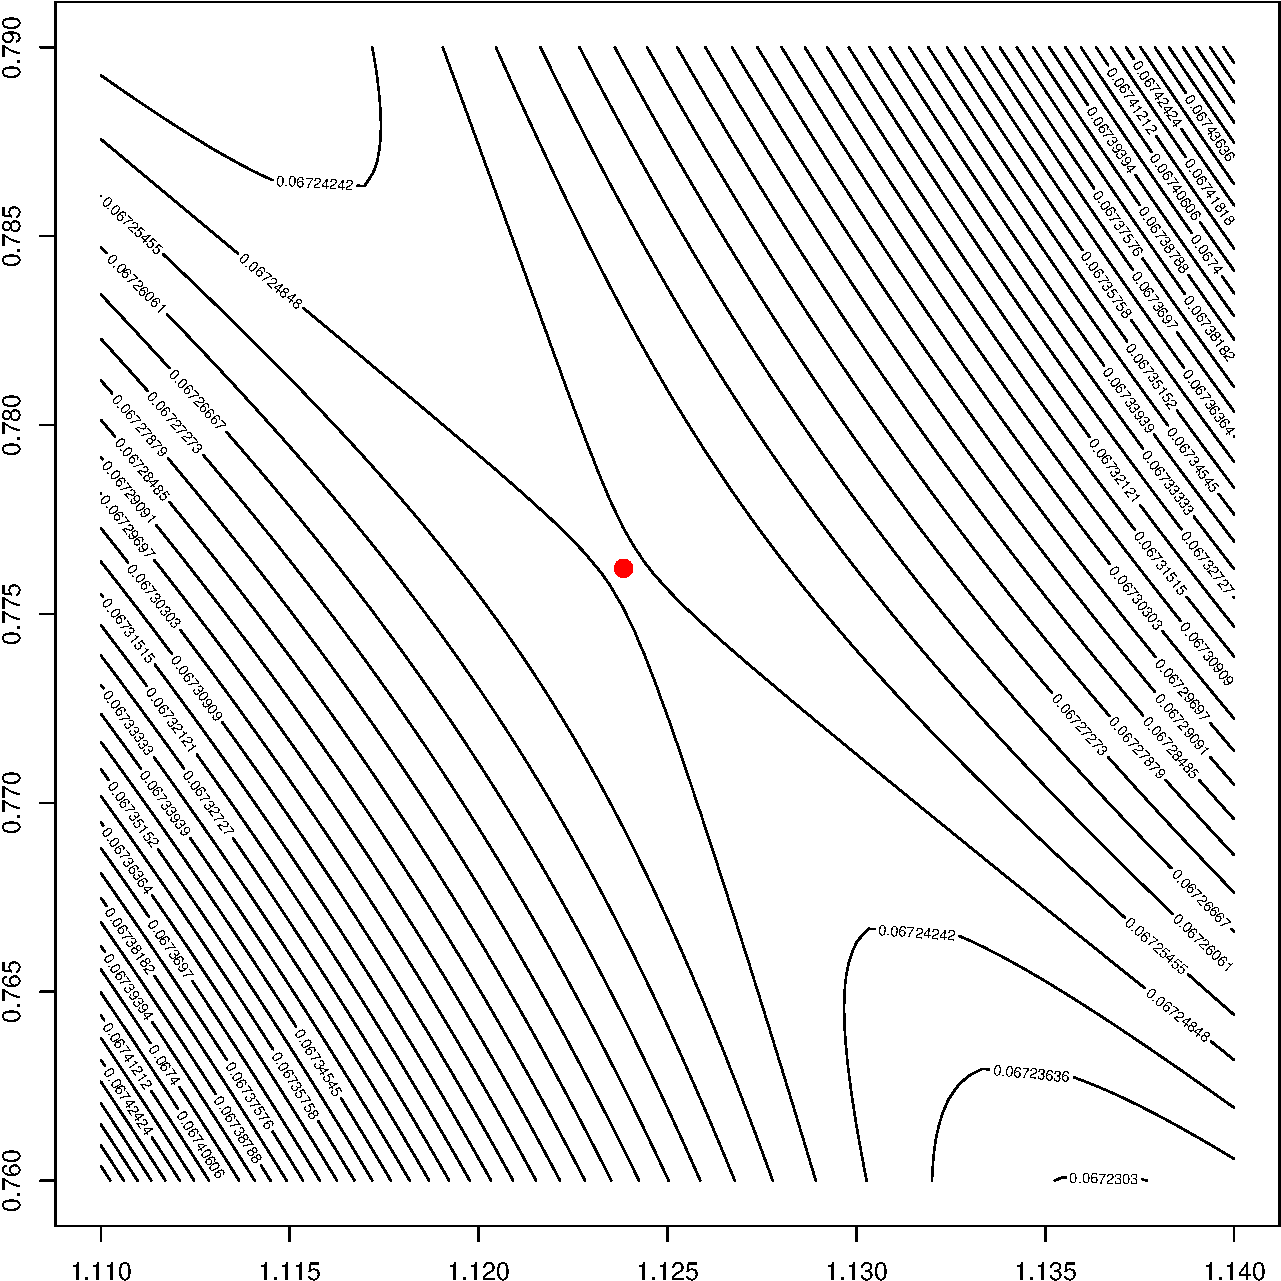
\includegraphics{spaces_files/figure-pdf/contsecsad-1.pdf}

}

\caption{Contour Plot Second Saddlepoint}

\end{figure}%

\section{Another Look}\label{picsphere}

Remember that \(\rho(\theta)=\theta'B(\theta)\theta\). Thus
\(\sigma(\lambda\theta)=1-\lambda\rho(\theta)+\frac12\lambda^2\theta'\theta\),
and \[
\min_\lambda\sigma(\lambda\theta)=1-\frac12\frac{\rho^2(\theta)}{\theta'\theta}.
\] Thus we can minimize \(\sigma\) over \(\theta\) by maximizing
\(\rho\) over the unit circle
\(\mathcal{S}:=\{\theta\mid\theta'\theta=1\}\). This is a nice
formulation, because \(\rho\) is norm, i.e.~a homogeneous convex
function of \(\theta\). Consequently we have transformed the problem
from unconstrained minimization of the DC function (i.e.~difference of
convex functions) stress to that of maximization of a ratio of norms. In
turn this is equivalent to maximization of the convex function \(\rho\)
over the unit circle, or, again equivalently, over the unit ball, a
compact convex set. This transform was first used in MDS by De Leeuw
(\citeproc{ref-deleeuw_C_77}{1977a}), partly because it made the theory
developed by Robert (\citeproc{ref-robert_67}{1967}) available.

The levels sets \(\{\theta\mid\rho(\theta)=\kappa\}\) are the
\(\rho\)-circles defined by the norm \(\rho\). The corresponding
\(\rho\)-balls \(\{\theta\mid\rho(\theta)\leq\kappa\}\) are closed and
nested convex sets containing the origin. Thus we want to find the
largest \(\rho\)-circle that still intersects \(\mathcal{S}\). The
similarity with the geometry of eigenvalue problems is obvious.

In our example we know that the global optimum of stress is at
(1.3938469, 0), and if we project that point on the circle it becomes
(1, 0). The corresponding optimal \(\rho\) is 1.3938469. Figure
@ref(fig:rhocontour) gives the contourplot for \(\rho\), with the outer
\(\rho\)-circle corresponding with the optimal value. The fact that the
optimal value contour is disjoint from the interior of \(\mathcal{S}\)
is necessary and sufficient for global optimality (Dür, Horst, and
Locatelli (\citeproc{ref-dur_horst_locatelli_98}{1998})). Notice the
sharp corners in the contour plot, showing the non-diffentiability of
\(\rho\) at the points where \(d_{12}(\theta)=0\). We could also look
for the minimum of \(\rho\) on the unit circle, which means finding the
largest \(\rho\)-circle that touches \(\mathcal{S}\) on the inside.
Inspecting figure @ref(fig:rhocontour) shows that this will be a point
where \(\rho\) is not differentiable, i.e. a point with
\(d_{12}(\theta)=0\). This minimum \(\rho\) problem does not make much
sense in the context of multidimensional scaling, however, and it not
related directly to the minimization of stress.

\begin{figure}[H]

{\centering 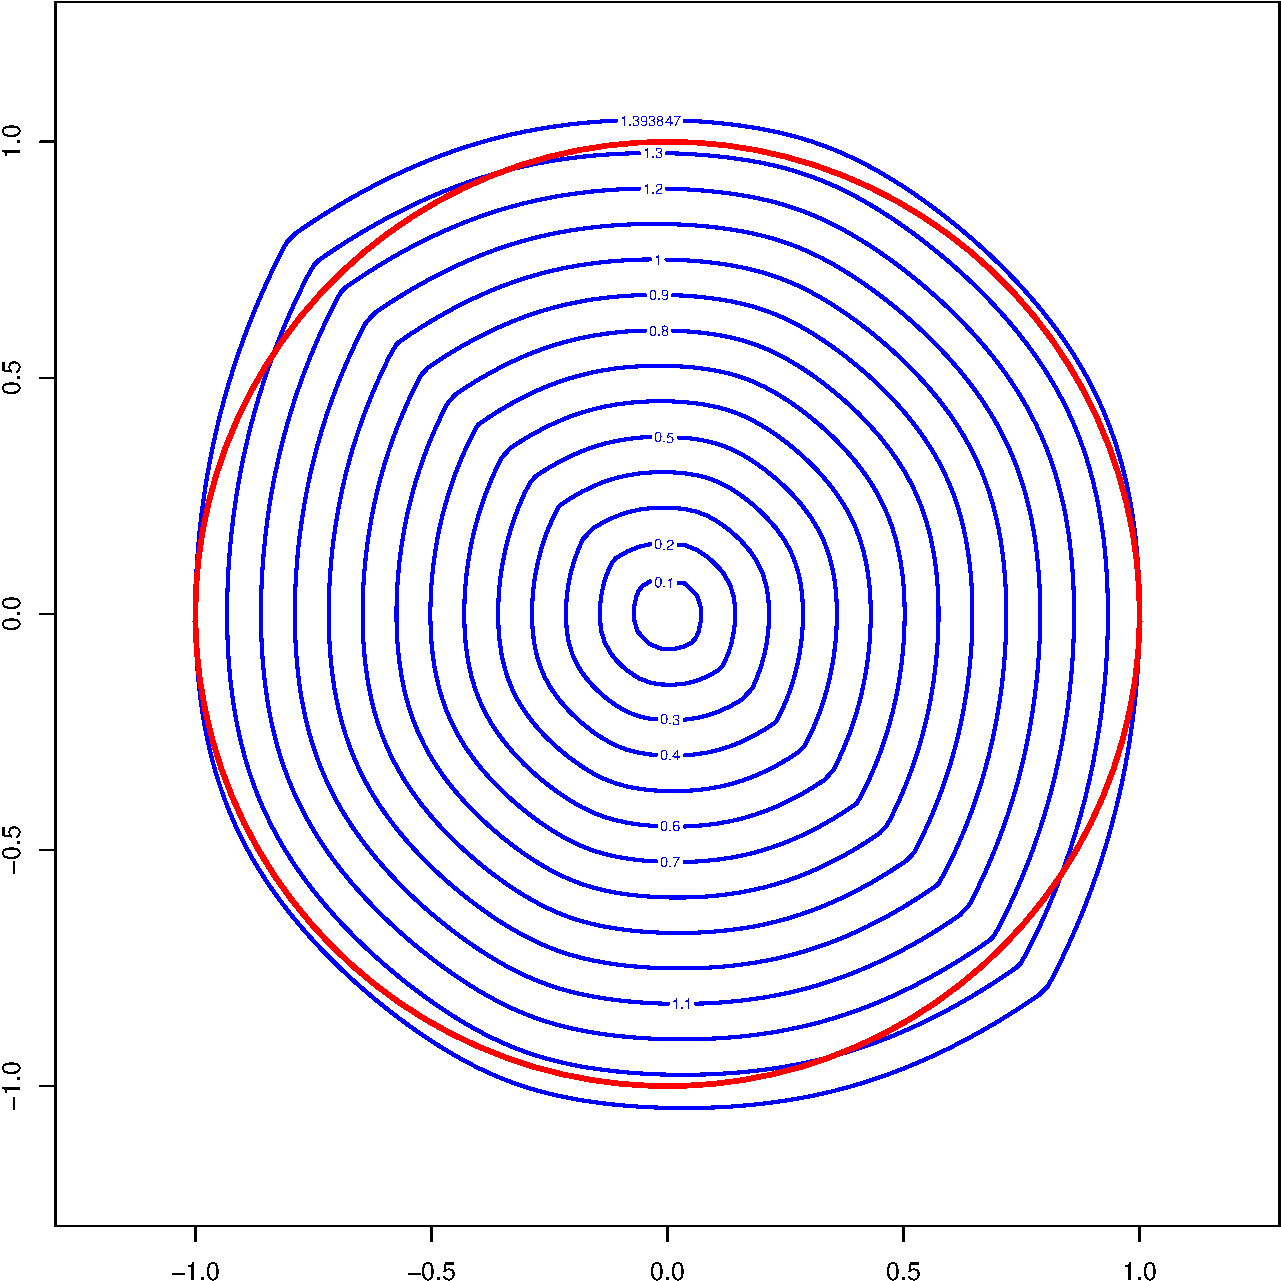
\includegraphics{spaces_files/figure-pdf/rhocontour-1.pdf}

}

\caption{Contour Plot for Rho}

\end{figure}%

\section{A Final Look}\label{picline}

Now that we know that the MDS problem is equivalent to maximizing
\(\rho\) on the unit circle, we can use nonlinear coordinates
\((\theta_1,\theta_2)=(\sin\xi,\cos\xi)\) to reduce the problem to a
one-dimensional unconstrained one in, say, ``circle space'\,'. Thus,
with the same abuse of notation as for stress,
\(\rho(\xi):=\rho(\sin\xi,\cos\xi)\), and we have to maximize \(\rho\)
over \(0\leq\xi\leq\pi\).

In figure @ref(fig:rhononlinearplot) we have plotted \(\rho\) as a
function of \(\eta\). There are blue vertical lines at the three local
minima in coefficient space, red vertical lines at the stationary
points, and a green vertical line where \(d_{12}(\xi)=0\). Note that in
circle space stress has both multiple local minima and multiple local
maxima.

\begin{figure}[H]

{\centering 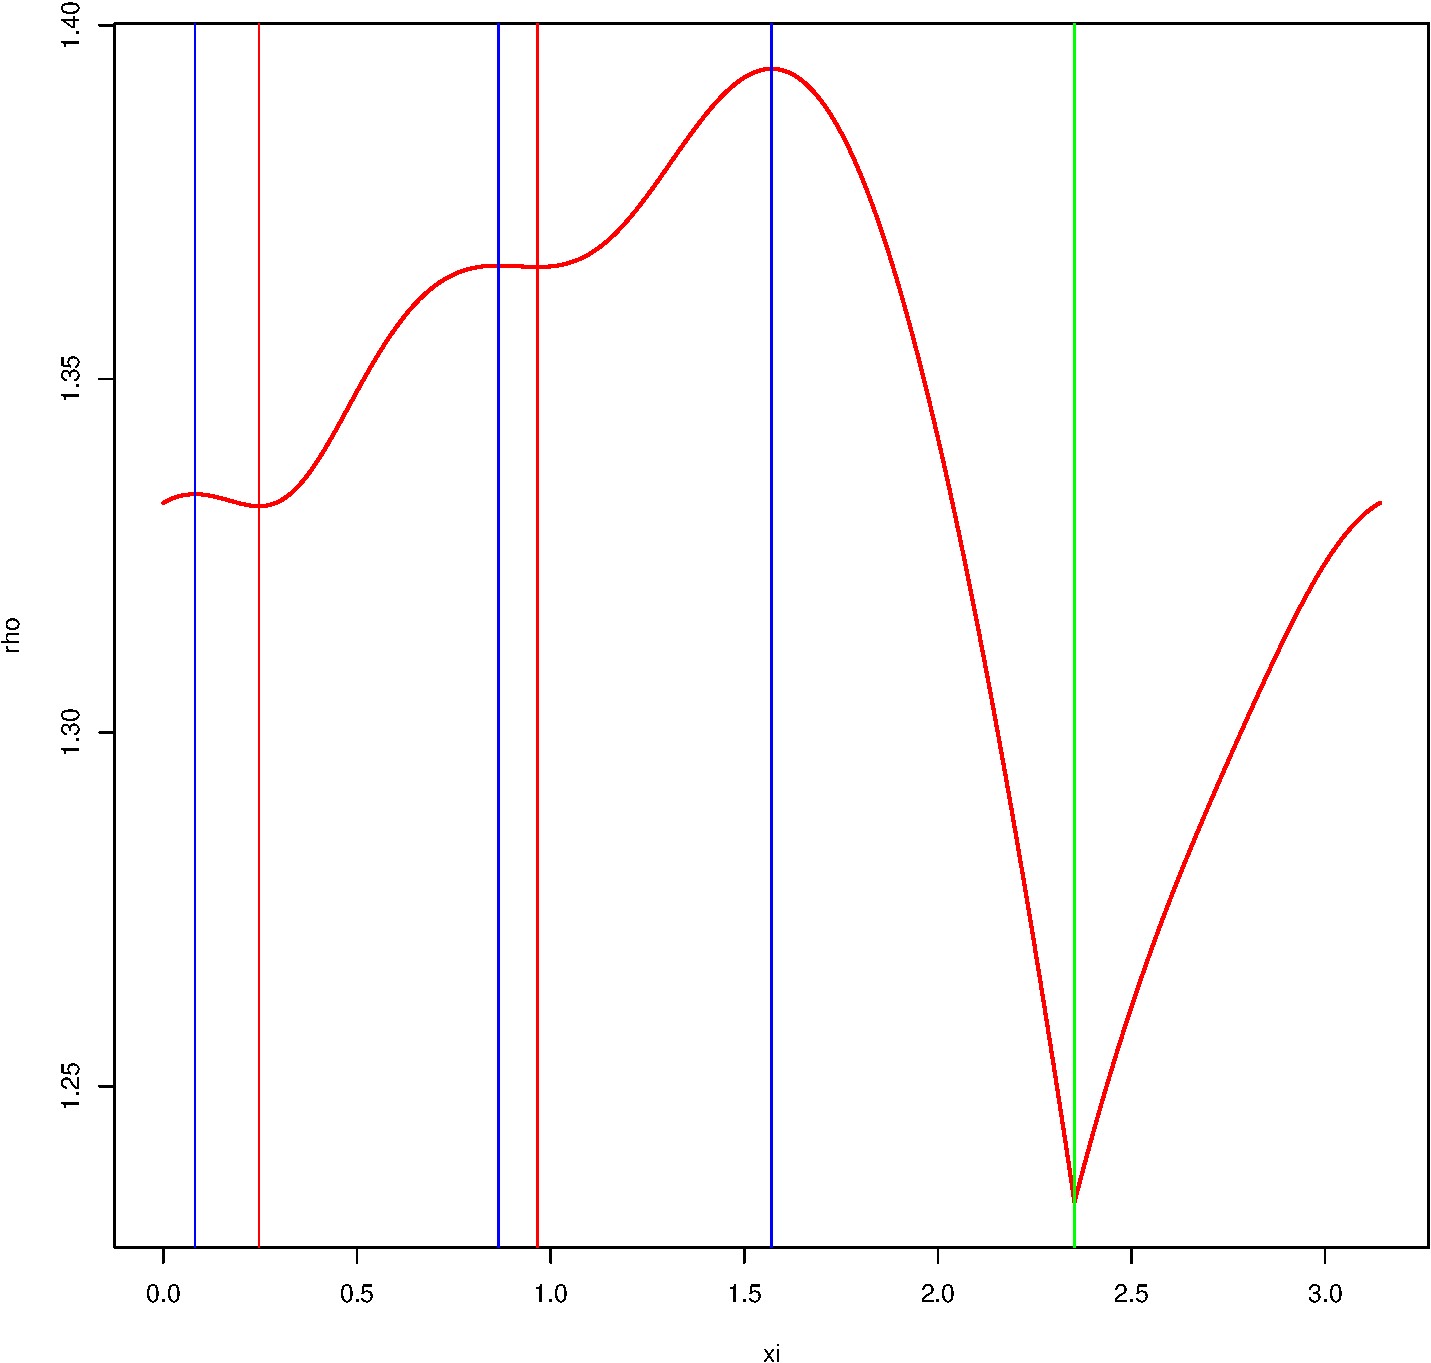
\includegraphics{spaces_files/figure-pdf/rhononlinearplot-1.pdf}

}

\caption{One-dimensional Rho}

\end{figure}%

From lemma xxx we see that the second derivative
\(\mathcal{D}^2\rho(\xi)\) is equal to
\(\mathbf{tr}\ H(\xi)-\rho(\xi)\). For the three local minima in
coordinate space we find second derivatives 0, 0, 0 in circle space,
i.e.~they are properly converted to local maxima. The two stationary
points in coordinate space have second derivatives 0, 0, and are turned
into local minima.

For more general cases, with a basis of \(n\) configurations, we know
from Lyusternik and Schnirelmann
(\citeproc{ref-lyusternik-schnirelmann_34}{1934}) that a continuously
differentiable even function on the unit sphere in \(\mathbb{R}^n\) has
at least \(n\) distinct pairs of stationary points.

\section{Discussion}\label{discussion}

Note that we have used \(\sigma\) for three different functions. The
first one with argument \(Z\) is defined on \emph{configuration space},
the second one with argument \(\gamma\) on \emph{coefficient space}, and
the third one with argument \(\theta\) also on \emph{coefficient space}.
This is a slight abuse of notation, rather innocuous, but we have to
keep it in mind.

From lemma xxx we see that
\(\mathcal{D}\sigma(X)=\mathcal{D}\sigma(Y)=0\) then
\(\mathcal{D}\sigma(1,0)=\mathcal{D}\sigma(0,1)=0\). Thus stationary
points in configuration space are preserved as stationary points in
coefficient space, but the reverse implication may not be true. If
\(\mathcal{D}^2\sigma(X)\) and \(\mathcal{D}^2\sigma(Y)\) are positive
semi-definite, then so are \(\mathcal{D}^2\sigma(1,0)\) and
\(\mathcal{D}^2\sigma(0,1)\). Thus local minima are preserved. But it is
entirely possible that \(\mathcal{D}^2\sigma(X)\) and/or
\(\mathcal{D}^2\sigma(Y)\) are indefinite, and that
\(\mathcal{D}^2\sigma(1,0)\) and/or \(\mathcal{D}^2\sigma(0,1)\) are
positive semi-definite. Thus saddle points in configuration space can be
mapped into local minima in coefficient space. As we will see this
actually happens with \(Y\), the equilateral triangle with center, in
our example.

\section{Coordinates}\label{coordinates}

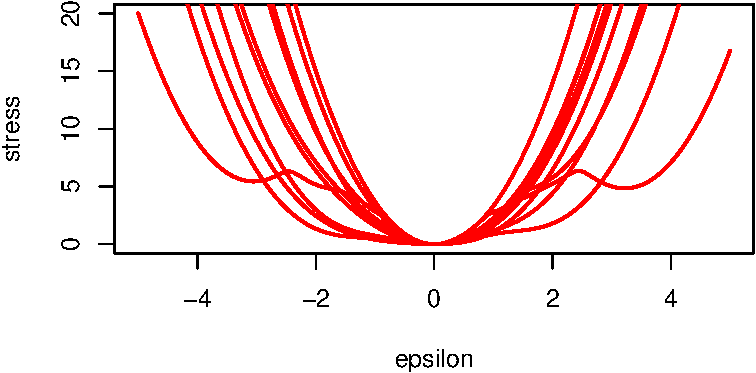
\includegraphics{spaces_files/figure-pdf/coordinates1-1.pdf}

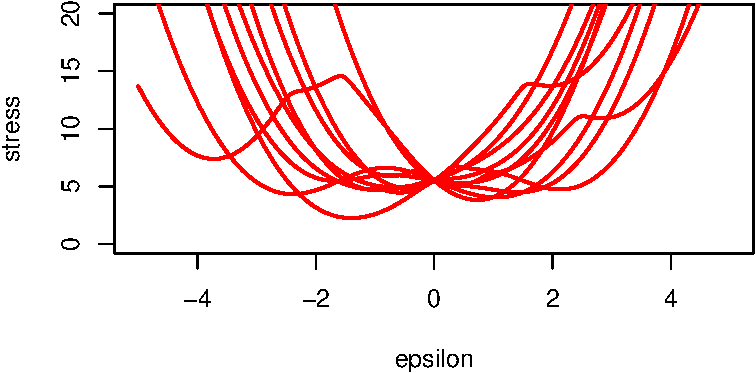
\includegraphics{spaces_files/figure-pdf/coordinates2-1.pdf}

Let's look at a small example with four points, all dissimilarities
equal, and all weights equal to one. There is a local minimum with four
points in the corners of a square, with stress equal to 0.0285955. And
there is another local minimum with three points forming an equilateral
triangle, and the fourth point in the center. This has stress 0.0669873.
We can compute stress for all points of the form \(\alpha X+\beta Y\),
where \(X\) and \(Y\) are the two local minima. Figure
@ref(fig:equalcontourplot) has a contour plot of
\(\sigma(\alpha,\beta)\), showing the local minima at \((1,0)\) and
\((0,1)\), and the local maximum at \((0,0)\).

\begin{figure}[H]

{\centering 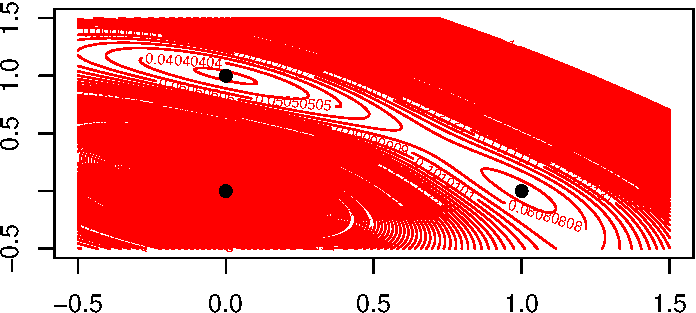
\includegraphics{spaces_files/figure-pdf/equalcontourplot-1.pdf}

}

\caption{Plane spanned by two local minima, equal dissimilarities}

\end{figure}%

Alternatively, we can plot stress on the line connecting \(X\) and
\(Y\). Note that although stress only has a local maximum at the origin
in configuration space, it can very well have local maxima if restricted
to lines. In fact on a line connecting two local minima there has to be
at least one local maximum.

\begin{figure}[H]

{\centering 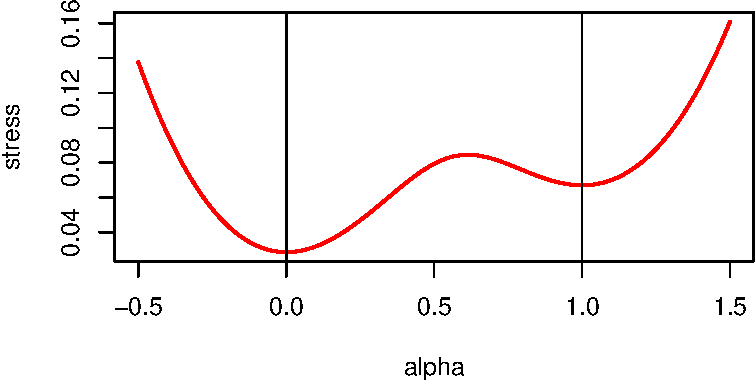
\includegraphics{spaces_files/figure-pdf/equallineplot-1.pdf}

}

\caption{Line connecting two local minima, equal dissimilarities}

\end{figure}%

A fundamental result, which forms the basis of chapter @ref(fullchapter)
in this book, is that \(\sigma\) is convex on \emph{Gramian Space},
i.e.~on the closed convex cone of all \(C\gtrsim 0\).

\bookmarksetup{startatroot}

\chapter{Classical Multidimensional
Scaling}\label{classical-multidimensional-scaling}

In the early days, exemplified by Messick and Abelson
(\citeproc{ref-messick_abelson_56}{1956}), the key mathematical result
used in MDS was Schoenberg's theorem (Schoenberg
(\citeproc{ref-schoenberg_35}{1935})), which was made available to
psychometricians by G. Young and Householder
(\citeproc{ref-young_householder_38}{1938}). Statisticians came to the
scene much later, not until Gower (\citeproc{ref-gower_66}{1966}).

Schoenberg's theorem gives necessary and sufficient conditions for a
symmetric, hollow, and non-negative matrix of dissimilarities to be the
distance matrix of \(n\) points in \(\mathbb{R}^p\). Several variations
of this basic theorem are possible (see Blumenthal
(\citeproc{ref-blumenthal_53}{1953}), chapter 43). We give the result in
the form popularized by W. S. Torgerson
(\citeproc{ref-torgerson_58}{1958}), with a simplified proof, using
notation and terminology due to Critchley
(\citeproc{ref-critchley_88}{1988}).

Classical scaling can be thought of as an independent MDS method, in
fact as the only MDS method available until the early 1960's. More
commonly these days it is a method to provide a generally excellent
starting point for iterative procedures to minimize stress.

\section{Algebra}\label{algebra}

\subsection{Torgerson Transform}\label{torgerson-transform}

The \emph{Torgerson transform} of a matrix is a linear function from the
space of real symmetric hollow matrices to the space of doubly-centered
real symmetric matrices defined as

\begin{equation}
\tau(S):=-\frac12 JSJ,
(\#eq:torgerson)
\end{equation}

with \(J\) the centering matrix \(I-\frac{1}{n}ee'\). For historical
reasons @(eq:torgerson) may be more familiar in elementwise notation.
Spelled out it is

\begin{equation}
\tau_{ij}(S)=-\frac12\{s_{ij}-s_{i\bullet}-s_{\bullet j}+s_{\bullet\bullet}\},
(\#eq:torgelem)
\end{equation}

where bullets are indices over which we average. The symbol \(\tau\) was
chosen by Critchley (\citeproc{ref-critchley_88}{1988}) to honor
Torgerson.

Some simple calculation with @ref(eq:torgelem), using the hollowness of
\(S\), gives

\begin{equation}
\tau_{ii}(S)+\tau_{jj}(S)-2\tau_{ij}(S)=s_{ij}.
(\#eq:torginv)
\end{equation}

Accordingly, Critchley (\citeproc{ref-critchley_88}{1988}) defines a
linear operator \(\kappa\) on the space of real symmetric matrices by
\(\kappa(S):=s_{ii}+s_{jj}-2s_{ij}\). From @ref(eq:torginv) we see that
\(\kappa(\tau(S))=S\). Also for all double-centered \(S\) we have
\(\tau(\kappa(S))=S\). Thus \(\tau\) and \(\kappa\) are mutually inverse
(Critchley (\citeproc{ref-critchley_88}{1988}), theorem 2.2).

\subsection{Schoenberg's Theorem}\label{schoenbergs-theorem}

\phantomsection\label{schoenberg}
There is an \(X\in\mathbb{R}^{n\times p}\) such that \(\Delta=D(X)\) if
and only if \(\tau(\Delta^{(2)})\) is positive semi-definite of rank
\(r\leq p\).

\begin{proof}
If \(\Delta\) are the distances of a column-centered \(p\)-dimensional
configuration \(X\), then the squared dissimilarities \(\Delta^{(2)}\)
are of the form \(ue'+eu'-2XX'\), where \(u_i=x_i'x_i^{\ }\) are the
squared row lengths. This implies \(\tau(\Delta^{(2)})=XX'\), which is
positive semi-definite of rank \(r=\text{rank}(X)\leq p\).

Conversely, suppose \(\tau(\Delta^{(2)})=XX'\). Applying \(\kappa\) to
both sides and using \(\kappa(XX')=D^{(2)}(X)\) gives
\(\Delta^{(2)}=D^{(2)}(X)\).
\end{proof}

Accordingly, we call a dissimilarity matrix \(\Delta\) \emph{Euclidean}
if it is symmetric, hollow, and non-negative and has
\(\tau(\Delta^{(2)})\gtrsim 0\). The \emph{dimension} of a Euclidean
dissimilarity matrix is the rank of \(\tau(\Delta^{(2)})\), which is
always less than or equal to \(n-1\).

\section{Approximation}\label{approximation}

\subsection{Low Rank Approximation of the Torgersen
Transform}\label{low-rank-approximation-of-the-torgersen-transform}

In classical MDS we minimize \begin{equation}
\sigma(X)=\text{tr}\ \left\{W(\tau(\Delta^{(2)})-XX')W\right\}^2
(\#eq:spapp)
\end{equation} over \(X\in\mathbb{R}^{n\times p}\), where \(W\) is a
square non-singular matrix of weights. The minimizer \(X\) for the loss
function in @ref(eq:spapp) is given by a slight variation of Eckart and
Young (\citeproc{ref-eckart_young_36}{1936}), discussed first by Keller
(\citeproc{ref-keller_62}{1962}). See also De Leeuw
(\citeproc{ref-deleeuw_R_74c}{1974}) and the generalizations to
rectangular and singular weight matrices in De Leeuw
(\citeproc{ref-deleeuw_A_84b}{1984c}). The solution is
\(X=W^{-1}K\Lambda\), where \(K\) are the normalized eigenvectors
corresponding with the \(p\) largest eigenvalues of the positive part of
\(W(\tau(\Delta^{(2)})W\) (i.e.~the matrix that results by replacing the
negative eigenvalues with zeroes). Thus the rank of the solution \(X\)
is equal to the minimum of \(p\) and the number of positive eigenvalues
of \(\tau(\Delta^{(2)}\).

In the original versions of classical scaling (W. S. Torgerson
(\citeproc{ref-torgerson_52}{1952}), W. S. Torgerson
(\citeproc{ref-torgerson_58}{1958})) there are no weights and the
problem that the Torgerson transform may be indefinite is ignored. In
fact, going from \(\tau(\Delta^{(2)}\) to \(X\) is done by ``any method
of factoring'', including the centroid method, so no specific loss
function is minimized.

The loss function @ref(eq:spapp) has been called, somewhat jokingly,
\emph{strain} by Takane, Young, and De Leeuw
(\citeproc{ref-takane_young_deleeuw_A_77}{1977}), mainly because
\emph{stress} and \emph{sstress} had already been taken. Stress is a
weighted least squares loss function defined on the distances, sstress
on the squared distances, and strain on the inner products.

\subsection{Minimization of Strain}\label{minimization-of-strain}

It may be considered a disadvantage of the classical approach, even if
it is described as the minimization of strain, that the MDS equations
are \(\Delta^{(2)}= D^{(2)(X)}\) while loss is measured on the scalar
products and not the distances or the squared distances.

It was first pointed out by De Leeuw and Heiser
(\citeproc{ref-deleeuw_heiser_C_82}{1982}) that strain can also be
written as a loss function defined on the squared distances. In fact
strain is equal to \begin{equation}
\sigma(X)=\frac14\text{tr}\ \left\{WJ(\Delta^{(2)}-D^{(2)}(X))JW\right\}^2,
(\#eq:strainer)
\end{equation} i.e.~to an appropriately weighted version of sstress.

An advantage of the classical scaling approach via minimizing strain is
that there is no local minimum problem. Finding the optimal
configuration is an eigenvalue problem, which allows us to find the
global minimum. This has not been emphasized enough, so I'll emphasize
it here once again. If iterative basic MDS algorithms use the classical
minimum strain solution as their starting point, then they start at the
global minimum of a related loss function. Since they are descent
algorithms they will improve their own loss functions, but having such
an excellent starting point means they avoid many local minima.

Another advantage of the loss function formulation in
@ref\{eq:strainer\} is that it is immediately obvious how to generalize
classical scaling when there are missing data or when there is only rank
order information. As with stress and sstress we minimize strain over
both the configuration \(X\) and the missing information.

\subsection{Approximation from Below}\label{approximation-from-below}

Suppose the Torgerson transform \(\tau(\Delta^{(2)}\) is PSD of rank
\(r\), with eigen decomposition \(K\Lambda^2 K'\), and, using the
largest \(p\) eigenvalues with corresponding eigenvectors, define
\(C_p:=K_p\Lambda_p^2 K_p'\). Then, in the Loewner order, \[
C_1\lesssim C_2\lesssim\cdots\lesssim C_r=\tau(\Delta^{(2)}).
\] Define \(X_p=K_p\Lambda_p\). Then applying Critchley's inverse
Torgerson transform \(\kappa\) it follows from \ldots{} that elementwise
\[
D^{(2)}(X_1)\leq D^{(2)}(X_2)\leq\cdots\leq D^{(2)}(X_r)=\Delta^{(2)},
\] and thus also \[
D(X_1)\leq D(X_2)\leq\cdots\leq D(X_r)=\Delta.
\] Thus in the PSD case classical scaling we approximate the
dissimilarities \emph{from below}. This result is implicit in Gower
(\citeproc{ref-gower_66}{1966}) and explicit in De Leeuw and Meulman
(\citeproc{ref-deleeuw_meulman_C_86}{1986}) and Meulman
(\citeproc{ref-meulman_86}{1986}).

If \(\tau(\Delta^{(2)}\) is not psd then

\[
D(X_1)\leq D(X_2)\leq\cdots\leq D(X_p)=\cdots=D(X_{n-1})\geq\Delta.
\]

Benzecri plot

\bookmarksetup{startatroot}

\chapter{Minimization of Basic Stress}\label{minstr}

\section{Gradient Methods}\label{gradient-methods}

The initial algorithms for nonmetric MDS Kruskal
(\citeproc{ref-kruskal_64b}{1964b}) and Guttman
(\citeproc{ref-guttman_68}{1968}) were gradient methods. Thus the
gradient, or vector of partial derivatives, was computed in each
iteration step, and a step was taken in the direction of the negative
gradient (which is also known as the direction of steepest descent).

Informally, if \(f\) is differentiable at \(x\) then
\(f(x+h)\approx f(x)+h'\mathcal{D}f(x)\) and the direction \(h\) that
minimizes the diferential (the second term) is
\(-\mathcal{D}f(x)/\|\mathcal{D}f(x)\|\), the normalized negative
gradient. Although psychometricians had been in the business of
minimizing least squares loss functions in the linear and bilinear case,
this result for general nonlinear functions was new to them. And I, and
probably many others, hungrily devoured the main optimization reference
in Kruskal (\citeproc{ref-kruskal_64b}{1964b}), which was the excellent
early review by Spang (\citeproc{ref-spang_62}{1962}).

Kruskal's paper also presents an elaborate step-size procedure, to
determine how far we go in the negative gradient direction. In the long
and convoluted paper Guttman (\citeproc{ref-guttman_68}{1968}) there is
an important contribution to gradient methods in basic MDS. Let's ignore
the complications arising from zero distances, which is after all what
both Kruskal and Guttman do as well, and assume all distances at
configuration \(X\) are positive. Then stress is differentiable at
\(X\), with gradient

\[
\nabla\sigma(X)=
-\sum_{i=1}^n\sum_{j=1}^nw_{ij}(\delta_{ij}-d_{ij}(X))\frac{1}{d_{ij}(X)}
(e_i-e_j)(x_i-x_j)'
\]

Geometrical interpretation - Gleason, Borg-Groenen p 20

Guttman C-matrix

Ramsay C-matrix

\subsection{Step Size}\label{step-size}

\subsubsection{Kruskal Step Size}\label{kruskal-step-size}

elaborate

\subsubsection{Guttman Step Size}\label{guttman-step-size}

constant

\subsubsection{Cauchy Step Size}\label{cauchy-step-size}

In the classical version of the steepest descent method we choose the
step-size \(\alpha\) by minimizing \(h(\alpha)=f(x+\alpha y)\) over
\(\alpha\)

\[
d_+h(\alpha;\beta)=\lim_{\epsilon\downarrow 0}\frac{f(x+(\alpha+\epsilon\beta)y)-f(x+\alpha y)}{\epsilon}=\beta\ d_+f(x+\alpha y;y)
\] or local minimum closest to zero

Newton version

\[
d_+^2h(\alpha;\beta,\gamma)=\beta\gamma d_+^2f(x+\alpha y;y,y)
\]

\subsubsection{Majorization Step Size}\label{majorization-step-size}

Lagrange form of the remainder

\(e(\epsilon)=\eta^2(X+\epsilon Y)\) \(r(\epsilon)=\rho(X+\epsilon Y)\)
\(s(\epsilon)=\sigma(X+\epsilon Y)=1-r(\epsilon)+\frac12e(\epsilon)\)

\[
r(\epsilon)\geq r(0)+r'(0)\epsilon
\] \[
e(\epsilon)=e(0)+e'(0)\epsilon+\frac12 e''(0)\epsilon^2
\] \[
s(\epsilon)\leq s(0)+s'(0)\epsilon+\frac12 e''(0)\epsilon^2
\] \[
\hat\epsilon=\frac{s'(0)}{e''(0)}
\] underestimates newton step

\[
r(\epsilon)\geq r(0)+\epsilon\ r'(0)+\frac12\epsilon^2\min_{0\leq \xi\leq\epsilon}r''(\xi)
\] \[
\hat\epsilon=\frac{s'(0)}{e''(0)-\min_{0\leq \xi\leq\epsilon}r''(\xi)}
\]

\[
r''(\xi)=\mathcal{D}^2\sigma(X+\xi Y;Y,Y)
\]

\section{Initial Configurations}\label{initial-configurations}

Random

L

Torgerson

Guttman

\section{On MM Algorithms}\label{apmajmin}

The term \emph{majorization} is used in mathematics in many different
ways. In this book we use it as a general technique for the construction
of \emph{stable} iterative minimization algorithms. An iterative
minimization algorithm is stable if it decreases the objective function
in each iteration.

Ortega, Rheinboldt Weber Bohning, Lindsay Vosz, Eckart

Special cases of majorization had been around earlier, most notably the
smacof algorithm for MDS and the EM algorithm for maximum likelihood
with missing data, but in full generality majorization was first
discussed in De Leeuw (\citeproc{ref-deleeuw_C_94c}{1994}) and Heiser
(\citeproc{ref-heiser_95}{1995}).

Majorization can be used to construct minimization methods, while
minorization can construct maximization methods. This cleverly suggests
to use the acronym MM algorithms for this class of techniques. An
excellent comprehensive account of MM algorithms is Lange
(\citeproc{ref-lange_16}{2016}). Another such account is slowly growing
in one of the companion volumes in this series of personal research
histories ((\citeproc{ref-deleeuw_B_21b}{\textbf{deleeuw\_B\_21b?}})).

Here we just give a quick introduction to majorization. Suppose \(f\) is
a real-valued function on \(X\subseteq\mathbb{R}^n\). Then a real-valued
function \(g\) on \(X\otimes X\) is said to majorize \(f\) on \(X\) if

\begin{equation}
g(x,y)\geq f(x)\qquad\forall (x,y)\in X\otimes X,
(\#eq:majorineq)
\end{equation}

and

\begin{equation}
g(y,y)=f(y)\qquad\forall y\in X.
(\#eq:majoreq)
\end{equation}

Thus for each \(y\in X\) the function \(g(\bullet,y)\) lies above \(f\),
and it touches \(f\) from above at \(x=y\). Majorization is
\emph{strict} if \(g(x,y)=f(x)\) if and only if \(x=y\), i.e.~if \(y\)
is the only point in \(X\) where \(g(\bullet,y)\) and \(f\) touch.

A \emph{majorization algorithm} to minimize \(f\) on \(X\) starts with
an initial estimate, and then updates the estimate in iteration \(k\) by

\begin{equation}
x^{(k+1)}\in\mathop{\text{argmin}}_{x\in X}g(x,x^{(k)}),
(\#eq:majoralg)
\end{equation}

with the understanding that the algorithms stops when
\(x^{(k)}\in\mathop{\text{argmin}}_{x\in X}g(x,x^{(k)})\).

If we do not stop we have an infinite sequence satisfying the
\emph{sandwich inequality}

\begin{equation}
f(x^{(k+1)})\leq g(x^{(k+1)},x^{(k)})\leq g(x^{(k)},x^{(k)})=f(x^{(k)}).
(\#eq:sandwich)
\end{equation}

The first inequality in this chain comes from @ref(eq:majorineq). It is
strict when majorization is strict. The second inequality comes from
@ref(eq:majoralg), and it is strict if \(g(\bullet,y)\) has a unique
minimum on \(X\) for each \(y\).

Necessary conditions through MM

\section{Smacof Algorithm}\label{smacof-algorithm}

\subsection{Guttman Transform}\label{propguttman}

The Guttman Transform is named to honor the contribution of Louis
Guttman to non-metric MDS (mainly, but by no means exclusively, in
Guttman (\citeproc{ref-guttman_68}{1968})). Guttman introduced the
transform in a slightly different way, and partly for different reasons.
In chapter @ref(minstr) we shall see that the Guttman Transform plays a
major role in defining and understanding the \(\textrm{smacof}\)
algorithm.

The \emph{Guttman Transform} of a configuration \(X\) is defined as
\begin{equation}
\Gamma(X):=V^+B(X)X,
(\#eq:guttrans)
\end{equation} which is simply equal to \(\Gamma(X)=n^{-1}B(X)X\) if all
weights are equal. For some purposes it is useful to think of
\(V^+B(X)X\) as a function of the weights, the dissimilarities, and the
configuration (see, for exam0ple, chapter @ref(chinverse)), but we
reserve the name Guttman transform for a map from
\(\mathbb{R}^{n\times p}\) into \(\mathbb{R}^{n\times p}\) .

What we have called \(B(X)\) is what Guttman calls the \emph{correction
matrix} or \emph{C-matrix} (see De Leeuw and Heiser
(\citeproc{ref-deleeuw_heiser_C_77}{1977}) for a comparison).

Completing the square in equation @ref(eq:propmatexp) gives
\begin{equation}
\sigma(X)=1+\eta^2(X-\Gamma(X))-\eta^2(\Gamma(X)),
(\#eq:gutsquare)
\end{equation} which shows that \begin{equation}
1-\eta^2(\Gamma(X))\leq\sigma(X)\leq 1+\eta^2(X-\Gamma(X)).
(\#eq:propsbounds)
\end{equation}

Note that it follows from @ref(eq:propsbounds) that
\(\sigma(X)\geq 1-\eta^2(\Gamma(X))\), with equality if and only if
\(X=\Gamma(X)\).

The Guttman transform is

\begin{itemize}
\item
  \emph{self-scaling} (a.k.a. homogeneous of degree zero) because
  \(\Gamma(\alpha X)=\Gamma(X)\) for all \(-\infty<\alpha<+\infty\).
  With our definition @ref(eq:bdef) of \(B(X)\) we also have
  \(\Gamma(0)=0\).
\item
  \emph{self-centering}, because \(\Gamma(X+e\mu')=\Gamma(X)\) for all
  \(\mu\in\mathbb{R}^p\).
\item
  Bounded
\item
  Lipschitz
\end{itemize}

::: \{ ,proof\} We already know, from the CS inequality, that
\begin{equation}
\rho(X)\leq\eta(X).
(\#eq:csagain)
\end{equation}

With the Guttman transform in hand we can apply CS once more, and find

\begin{equation}
\rho(X)=\text{tr}\ X'B(X)X=\text{tr}\ X'V\Gamma(X)\leq\eta(X)\eta(\Gamma(X))
(\#eq:csagainagain)
\end{equation}

Note that the Guttman transform is bounded. In fact, using the Euclidean
norm throughout, \[
\Gamma(X)\leq\|V^+\|\|B(X)X\|
\] Now \[
B(X)X=\mathop{\sum\sum}_{1\leq i<j\leq n}w_{ij}\delta_{ij}\frac{x_i-x_j}{d_{ij}(X)}(e_i-e_j),
\] and thus

\[
\|B(X)X\|\leq\mathop{\sum\sum}_{1\leq i<j\leq n}w_{ij}\delta_{ij}\left\|\frac{x_i-x_j}{d_{ij}(X)}\right\|\|e_i-e_j\|=\sqrt{2}\mathop{\sum\sum}_{1\leq i<j\leq n}w_{ij}\delta_{ij},
\] and \[
\|\Gamma(X)\|\leq\sqrt{2}\|V^+\|\mathop{\sum\sum}_{1\leq i<j\leq n}w_{ij}\delta_{ij}.
\] In fact \[
B(X)X-B(Y)Y=\mathop{\sum\sum}_{1\leq i<j\leq n}w_{ij}\delta_{ij}\left\{\frac{x_i-x_j}{d_{ij}(X)}-\frac{y_i-y_j}{d_{ij}(Y)}\right\}(e_i-e_j),
\] and thus \[
\|\Gamma(X)-\Gamma(Y)\|\leq 2\|V^+\|
\mathop{\sum\sum}_{1\leq i<j\leq n}w_{ij}\delta_{ij},
\] and thus the Guttman transform is Lipschitz. ::: ;'\,'\,'\,'ytyh
\#\#\# Subdifferentials

\subsection{Derivative}\label{derivative}

The basic smacof algorithm, which is the main building block for most of
the MDS techniques discussed in this book, updates the configuration
\(X^{(k)}\) in iteration \(k\) by

\begin{equation}
X^{(k+1)}=\Gamma(X^{(k)})=V^+B(X^{(k)})X^{(k)}.
(\#eq:smacofupdate)
\end{equation}

so that first \(X^{(1)}=\Gamma(X^{(0)})\), then
\(X^{(2)}=\Gamma(X^{(1)})=\Gamma(\Gamma(X^{(0)}))\), and generally
\(X^{(k)}=\Gamma^k(X^{0}),\) where \(\Gamma^k\) is the k-times
composition (or iteration) of \(\Gamma.\)

We shall show in this chapter that as \(k\rightarrow\infty\) both\\
\(\sigma(X^{(k+1)})-\sigma(X^{(k)})\rightarrow 0\), and
\(\eta^2(X^{(k)}-X^{(k+1)})=(X^{(k+1)}-X^{(k)})'V(X^{(k+1)}-X^{(k)})\rightarrow 0\).
The iterations stop either if
\(\sigma(X^{(k)})-\sigma(X^{(k+1)})<\epsilon\) or if
\(\eta^2(X^{(k)}-X^{(k+1)})<\epsilon\), where the \(\epsilon\) are small
cut-off numbers chosen by the user, or if we reach a user-defined
maximum number of iterations, and we give up on convergence. The user
also chooses if the stop criterion is based on function value changes or
configuration changes.

Some quick remarks on implementation. We only have to compute \(V^+\)
once, but premultiplying by a full symmetric matrix in each iteration
does add quite a few multiplications to the algorithm. If all \(w_{ij}\)
are one, then \(V^+=\frac{1}{n}J\) and thus
\(\Gamma(X^{(k)})=\frac{1}{n}B(X^{(k)})X^{(k)}\). In fact we do not even
have to carry out this division by \(n\), because the basic algorithm is
\emph{self scaling}. which means in this context that
\(\Gamma(\alpha X)=\Gamma(X)\) for all \(\alpha\geq 0\).

\subsection{Global Convergence}\label{global-convergence}

The iterations in @ref(eq:smacofupdate) start at some \(X^{(0)}\) and
then generate five sequences of non-negative numbers. Define
\(\lambda(X):=\rho(X)/\eta(X)\) and \(\Gamma(X):=\eta^2(X-\Gamma(X))\).
The five sequences we will look at are

\begin{align}
\begin{split}
\sigma_k&:=\sigma(X^{(k)}),\\
\rho_k&:=\rho(X^{(k)}),\\
\eta_k&:=\eta(X^{(k)}),\\
\lambda_k&:=\lambda(X^{(k)}),\\
\Gamma_k&:=\Gamma(X^{(k)}),
\end{split}
(\#eq:smacofseq)
\end{align}

Depend on \(X^{(0)}\)

Zangwill

Argyros

\subsubsection{From the CS Inequality}\label{from-the-cs-inequality}

\phantomsection\label{smacoffunc}
~

\begin{enumerate}
\def\labelenumi{\arabic{enumi}.}
\item
  \(\sigma_k\) is a decreasing sequence, bounded below by 0.
\item
  \(\rho_k\), \(\eta_k\), amd \(\lambda_k\) are increasing sequences,
  bounded above by 1.
\item
  \(\Gamma_k\) is a null-sequence.
\end{enumerate}

To prove convergence of these sequences we slightly modify and extend
the proofs in De Leeuw (\citeproc{ref-deleeuw_C_77}{1977a}) and De Leeuw
and Heiser (\citeproc{ref-deleeuw_heiser_C_77}{1977}) (while I say to
myself: that's 44 years ago).

\begin{proof}
\leavevmode

\begin{enumerate}
\def\labelenumi{\arabic{enumi}.}
\item
  For each \(X\in\mathbb{R}^{n\times p}\) we have \(\rho(X)\leq\eta(X)\)
  and thus \(\lambda(X)\leq 1\).
\item
  For each \(X,Y\in\mathbb{R}^{n\times p}\) we have
  \(\rho(X)\geq\text{tr}\ X'B(Y)Y\) and thus
  \(\rho(X)\geq\text{tr}\ X'V\Gamma(Y)\). Taking \(X=\Gamma(Y)\) we see
  that \(\rho(X)\geq\eta^2(\Gamma(Y))\). Now
  \(\sigma(\Gamma(Y))=1-2\rho(\Gamma(Y))+\eta^2(\Gamma(Y))\leq 1-\eta^2(\Gamma(Y))\)
  and thus for all \(X\) \(\eta^2(\Gamma(X)) \leq 1\).
\item
  For each \(X\in\mathbb{R}^{n\times p}\) we have
  \(\rho(X)=\text{tr}\ X'B(X)X\) and thus
  \(\rho(X)\leq\eta(X)\eta(\Gamma(X))\) and thus
  \(\lambda(X)\leq\eta(\Gamma(X))\)
\end{enumerate}

\[
\rho(X^{(k)})=\text{tr}\ \{X^{(k)}\}'VX^{(k+1)}\leq\eta(X^{(k)})\eta(X^{(k+1)}),
\]

\[
\rho(X^{(k+1)})\geq\text{tr}\ \{X^{(k+1)}\}'B(X^{(k)})X^{(k)}=\eta^{2}(X^{(k+1)}),
\]

\[
\eta(X^{(k)})\leq\lambda(X^{(k)})\leq\eta(X^{(k+1)})
\]

and

\[
\rho(X^{(k)})\leq\frac{\eta(X^{(k)}}{X^{(k+1)}}\rho(X^{(k+1)})\leq\rho(X^{(k+1)})
\]
\end{proof}

\subsubsection{From Majorization}\label{from-majorization}

Smacof is based on the majorization, valid for all configurations \(X\)
and \(Y\),

\begin{equation}
\sigma(X)\leq 1+\eta^2(X-\Gamma(Y))-\eta^2(\Gamma(Y)),
(\#eq:upbmajineq)
\end{equation}

with equality if and only if \(X\propto Y\). If \(Y=\alpha X\) for some
\(\alpha\) then \begin{equation}
\sigma(X)=1+\eta^2(X-\Gamma(Y))-\eta^2(\Gamma(Y)),
(\#eq:upbmajeq)
\end{equation} and specifically we have @ref(eq:upbmajeq) if \(Y=X\).

Now suppose we have an \(Y\) with \(Y\not=\Gamma(Y)\). If
\(\eta^2(X-\Gamma(Y))\leq\eta^2(Y-\Gamma(Y))\) then

\begin{align}
\begin{split}
\sigma(X)%\leq 1+\eta^2(X-\Gamma(Y))-\eta^2(\Gamma(Y))\leq\\
&\leq 1+\eta^2(Y-\Gamma(Y))-\eta^2(\Gamma(Y))=\sigma(Y)
\end{split}
(\#eq:upbmajimp)
\end{align}

The obvious choice for \(X\) is \(X=\Gamma(Y)\), which makes
\(\eta^2(X-\Gamma(Y))=0\), and thus

\begin{equation}
\sigma(X)\leq 1-\eta^2(\Gamma(Y))<
1+\eta^2(Y-\Gamma(Y))-\eta^2(\Gamma(Y))=\sigma(Y)
(\#eq:upbmajmin)
\end{equation}

\subsubsection{From Ratio of Norms}\label{from-ratio-of-norms}

De Leeuw (\citeproc{ref-deleeuw_C_77}{1977a})

DC Algorithm

Robert

\subsection{Component Rotated Smacof}\label{mincomprot}

Consider the modified smacof iterations
\(\tilde X^{(k+1)}=X^{(k+1)}L^{(k+1)}\), where \(L^{(k+1)}\) are the
normalized eigenvectors of \(\{X^{(k+1)}\}^TVX^{(k+1)}\). Then

\[
\sigma(\tilde X^{(k)})=\sigma(X^{(k)})
\] Thus the modified update produces the same sequence of stress values
as the basic update. Also \[
\Gamma(\tilde X^{(k)})=\Gamma(X^{(k)})L^{(k)}
\] Thus \(\tilde X^{(k)}\) and \(X^{(k)}\) differ by a rotation for each
\(k\). It follows that we can actually compute \(\tilde X^{(k)}\) from
the basic sequence \(X^{(k)}\) by rotating the \(X^{(k)}\) to principal
components. Specifically if \(X_\infty\) is a subsequential limit of
\(X^{(k)}\) then the corresponding limit of \(\tilde X^{(k)}\) is
\(X_\infty\) rotated to principal components. Modifying the intermediate
updates is just a waste of time, we can simply rotate the final smacof
solution. And we should, as we explain in the next section,
@ref(minlocconv).

\subsection{Local Convergence}\label{minlocconv}

\[
\mathcal{D}\Gamma(X)(Y)=V^+\left\{B(X)Y-\mathop{\sum\sum}_{1\leq i<j\leq n} w_{ij}\frac{\delta_{ij}}{d_{ij}(X)}\left(\frac{\text{tr}\ Y'A_{ij}X}{d_{ij}^2(X)}\right)A_{ij}\right\}
\]

For any X: one zero eigenvalue \(\mathcal{D}\Gamma(X)(X)=0\)

If on \(\mathbb{R}^{n\times p}\) then an additional \(p\) zero
eigenvalues \(\mathcal{D}\Gamma(X)(e\mu^T)=0\)

For \(X=\Gamma(X)\) and \(M\) anti-symmetric: \(\frac12 p(p-1)E\) unit
eigenvalues \(\mathcal{D}\Gamma(X)(XM)=\Gamma(X)M=XM\)

\subsubsection{Cross Product Iterations}\label{cross-product-iterations}

Map of C into C. No rotational indeterminacy. Same stress sequence.

\[
C^{(k+1)}=V^+B(C^{(k)})C^{(k)}B(C^{(k)})V^+
\] Map of \(D\) into \(D\). Guttman transform as function of distances.
Not very nice.

\[
D^{(k+1)}:=D(X^{(k+1)})=D(\Gamma(X^{(k)}))
\]

\subsubsection{Rotation to PC}\label{rotation-to-pc}

We suppose the configfuration \(X\) is \(n\times p\), with rank \(p\).
If the singular value decomposition is \(X=K\Lambda L'\) then the
rotation to principle components is \(\Gamma(X):=K\Lambda=XL\). Thus
\(\mathcal{D}\Gamma(X)(Y)=YL+X\mathcal{D}L(X)(Y)\). So we need to
compute \(\mathcal{D}L(X)\), with \(L\) the right singular vectors of
\(X\), i.e.~the eigenvectors of \(X^TX\). We use the methods and results
from De Leeuw (\citeproc{ref-deleeuw_R_07c}{2007b}), which were applied
to similar problems in De Leeuw (\citeproc{ref-deleeuw_R_08b}{2008}), De
Leeuw and Sorenson (\citeproc{ref-deleeuw_sorenson_U_12b}{2012}), and De
Leeuw (\citeproc{ref-deleeuw_E_16p}{2016a}).

\phantomsection\label{minrotpc}
If the \(n\times p\) matrix has rank \(p\), singular value decomposition
\(X=K\Lambda L^T\), with all singular values different, then
\(\Gamma(X+\Delta)=\Gamma(X)+\Delta L+XLM+o(\|\Delta\|)\), where \(M\)
is antisymmetric with off-diagonal elements

\begin{equation}
m_{ij}=\frac{\lambda_is_{ij}+\lambda_js_{ji}}{\lambda_i^2-\lambda_j^2}.
(\#eq:minsvdmsolve)
\end{equation}

\begin{proof}
The proof involves computing the derivatives of the singular value
decomposition of \(X\), which is defined by the equations

\begin{align}
XL&=K\Lambda,(\#eq:minsvd1)\\
X^TK&=L\Lambda,(\#eq:minsvd2)\\
K^TK&=I,(\#eq:minsvd3)\\
L^TL&=LL^T=I.(\#eq:minsvd4)
\end{align}

We now perturb \(X\) to \(X+\Delta\), which perturbs \(L\) to
\(L+L_\Delta+o(\|\Delta\|)\), \(K\) to \(K+K_\Delta+o(\|\Delta\|)\), and
\(\Lambda\) to \(\Lambda+\Lambda_\Delta+o(\|\Delta\|)\). Substutute this
into the four SVD equations for \(X+\Delta\) and keep the linear terms.

\begin{align}
XL_\Delta+\Delta L&=K_\Delta\Lambda+K\Lambda_\Delta,(\#eq:minsvdperb1)\\
X^TK_\Delta+\Delta^TK&=L_\Delta\Lambda+L\Lambda_\Delta,(\#eq:minsvdperb2)\\
L_\Delta^TL+L^TL_\Delta&=0,(\#eq:minsvdperb3)\\
K_\Delta^TK+K^TK_\Delta&=0.(\#eq:minsvdperb4)
\end{align}

Define \(M:=L^TL_\Delta\) and \(N:=K^TK_\Delta\). Then equations
@ref(eq:minsvdperb3) and @ref(eq:minsvdperb4) say that \(M\) and \(N\)
are antisymmetric. Also define \(S:=K^T\Delta L\). Premultiplying
equation @ref(eq:minsvdperb1) by \(K^T\) and @ref(eq:minsvdperb2) by
\(L^T\) gives

\begin{align}
\Lambda M+S&=N\Lambda+\Lambda_\Delta,(\#eq:minsvdred1)\\
\Lambda N+S^T&=M\Lambda+\Lambda_\Delta.(\#eq:minsvdred2)
\end{align}

Either of these two equations gives, using the antisymmetry, and thus
hollowness, of \(M\) and \(N\), that \(\Lambda_\Delta=\text{diag}(S)\).
Define the hollow matrix \(U:=S-\text{diag}(S)\). Then

\begin{align}
\Lambda M-N\Lambda&=U,(\#eq:minsvdu1)\\
\Lambda N-M\Lambda&=U^T.(\#eq:minsvdu2)
\end{align}

Premultiply @ref(eq:minsvdu1) and postmultiply @ref(eq:minsvdu2) by
\(\Lambda\).

\begin{align}
\Lambda^2 M-\Lambda N\Lambda&=\Lambda U,(\#eq:minsvdu3)\\
\Lambda N\Lambda-M\Lambda^2&=U^T\Lambda.(\#eq:minsvdu4)
\end{align}

If we add these two equations we can solve for the off-diagonal elements
of \(M\) and find the expression in the theorem. Since \(L_\Delta=LM\)
this completes the proof.
\end{proof}

\subsection{Data Asymmetry}\label{datasym}

The non-basic situation in which there are asymmetric weights and/or
asymmetric dissimilarities in basic MDS is analyzed in De Leeuw
(\citeproc{ref-deleeuw_C_77}{1977a}), although it is just standard
linear least squares projection theory. We give a slightly different
partitionng ofd the sum of squares here. Note that it is not even
necessary that the weights and dissimilarities are hollow and/or
non-negative.

We decompose the weights and dissimilarities additively into a symmetric
and anti-symmetric part. Thus \(w_{ij}=w_{ij}^S+w_{ij}^A\) and
\(\delta_{ij}=\delta_{ij}^S+\delta_{ij}^A\). Now in general if \(A\) is
anti-symmetric and \(B\) is symmetric, then \(\text{tr}\ AB=0\). Also
their Hadamard (element-wise) product \(A*B\) is anti-symmetric, and the
Hadamard product of two anti-symmetric matrices is symmetric. Using
these rules gives after some calculation \begin{align}
\begin{split}
\sigma(X)&=\frac14\sum_{i=1}^n\sum_{j=1}^nw_{ij}(\delta_{ij}-d_{ij}(X))^2=\\&=\frac14\sum_{i=1}^n w_{ii}^{\ }\delta_{ii}^2+
\frac12\mathop{\sum\sum}_{1\leq i<j\leq n}w_{ij}^S\left\{\underline{\delta}_{ij}-d_{ij}(X)\right\}^2+\frac12\mathop{\sum\sum}_{1\leq i<j\leq n}\frac{w_{ij}w_{ji}}{w_{ij}^S}\{\delta_{ij}^A\}^2,
\end{split}(\#eq:partiunsym)
\end{align} where \begin{equation}
\underline{\delta}_{ij}:=\delta_{ij}^S+\frac{w_{ij}^A\delta_{ij}^A}{w_{ij}^S}.
(\#eq:defofunddelta)
\end{equation} Thus minimizing stress in the case of asymmetric weights
and dissimilarities, which even can be non-hollow and non-positive,
reduces to a symmmetric basic MDS problem for adjusted dissimilarities
defined by equation @ref(eq:defofunddelta). If the original weights and
dissimilarities are non-negative, then so are the weights \(w_{ij}^S\)
and the dissimilarities \(\underline{\delta}_{ij}\).

\subsection{Replications}\label{minrepl}

If there are replications in basic MDS we can use a simple partitioning
of stress to reduce the problem to standard form. We start with
\begin{equation}
\sigma(X)=\frac12\sum_{k=1}^m\mathop{\sum\sum}_{1\leq i<j\leq n}w_{ijk}(\delta_{ijk}-d_{ij}(X))^2.
\#(eq:inddiffstress)
\end{equation} Let \begin{align}
w_{ij\bullet}&=\sum_{k=1}^m w_{ijk}(\#eq:wbul1)\\
\delta_{ij\bullet}&=\frac{\sum_{k=1}^m w_{ijk}\delta_{ijk}}{w_{ij\bullet}}(\#eq:wbul2).
\end{align} Then \begin{equation}
\sigma(X)=\frac12\mathop{\sum\sum}_{1\leq i<j\leq n} w_{ij\bullet}(\delta_{ij\bullet}-d_{ij}(X))^2+\frac12\sum_{k=1}^m\mathop{\sum\sum}_{1\leq i<j\leq n} w_{ijk}(\delta_{ijk}-\delta_{ij\bullet})^2,
(\#eq:partinddiff)
\end{equation} and it suffices to minimize the first term, which is a
standard basic MDS problem.

In the nonmetric case, in which in principle each of the \(\Delta_k\)
can be transformed, we must alternate minimization of
\#ref(eq:inddiffstress) over the \(\Delta_k\) and minimization of
@ref(eq:partinddiff) over \(X\). In the case in which \(X_k\) is
different pover replications we use the methods of chapter
@ref(chindif).

\subsection{Negative Dissimilarities}\label{negative-dissimilarities}

\begin{equation}
\sigma(X)=1-\sum_{k\in\mathcal{K}_{1+}} w_k\delta_kd_k(X)
+\sum_{k\in\mathcal{K}_{1-}} w_k|\delta_k|d_k(X)+\frac12\sum_{k\in\mathcal{K}} w_kd_k^2(X)).
(\#eq:disneg)
\end{equation}

Split rho

Heiser (\citeproc{ref-heiser_91}{1991})

\subsection{Normalization}\label{normalization}

In actual computer output using the scaling in formula
@ref(eq:scaldiss1) and @ref(eq:scaldiss1) has some disadvantages. There
are, say, \(M\) non-zero weights. The summation in \#ref(eq:stressall)
is really over \(M\) terms only. If \(n\) is at all large the scaled
dissimilarities, and consequently the distances and the configuration,
will become very small. Thus, in actual computation, or at least in the
computer output, we scale our dissimilarities as
\(\frac12\mathop{\sum\sum}_{1\leq j<i\leq n} w_{ij}^{\ }\delta_{ij}^2=M\).
So, we scale our dissimilarities to one in formulas and to \(M\) in
computations. Thus the computed stress will b

In fact, we do not even use it in our computer programs, except at the
very last moment when we return the final stress after the algorithm has
completed.

\subsection{Unweighting}\label{minunweight}

Consider the general problem of minimizing a least squares loss
function, defined as \(f(x):=(x-y)'W(x-y)\) over \(x\) in some set
\(X\), where \(W\) is a symmetric weight matrix. Sometimes \(W\)
complicates the problem, maybe because it is too big, too full, too
singular, or even indefinite. We will use iterative majorization to give
\(W\) a more subordinate role. See also Kiers
(\citeproc{ref-kiers_97}{1997}) and Groenen, Giaquinto, and Kiers
(\citeproc{ref-groenen_giaquinto_kiers_03}{2003}).

Suppose \(z\) is another element of \(X\). Think of it as the current
best approximation to \(y\) that we have, which we want to improve. Then

\begin{align}
\begin{split}
f(x)&=(x-y)'W(x-y)\\
&=((x-z)+(z-y))'W((x-z)+(z-y))\\
&=f(z)+2(x-z)'W(z-y)+(x-z)'W(x-z)
\end{split}
(\#eq:unwgth)
\end{align}

Now choose a non-singular \(V\) such that \(W\lesssim V\) and define
\(u:=V^{-1}W(z-y)\). Then we have the majorization

\begin{equation}
f(x)\leq f(z)+2(x-z)'W(z-y)+(x-z)'V(x-z)=\\
f(z)+2(x-z)'Vu+(x-z)'V(x-z)=\\
f(z)+(x-(z-u))'V(x-(z-u))-u'Vu.
(\#eq:compsq)
\end{equation}

Here are some ways to choose \(V\). We use \(\lambda_{\text{max}}(W)\)
and \(\lambda_{\text{min}}(W)\) for the largest and smallest eigenvalues
of the symmetric matrix \(W\).

For any \(W\) we can choose \(V=\lambda_{\text{max}}(W)I\). Or, more
generally, \(V=\lambda_{\text{max}}(D^{-1}W)D\) for any positive
definite \(D\). If \(W\) is singular we can choose \(V=W+\epsilon D\)
for any positive definite \(D\). And in the unlikely case that \(W\) is
indefinite we can choose \(V=W+(\epsilon-\lambda_{\text{min}}(W))I\).
But if \(W\) is indefinite we have more serious problems.

In appendix @ref(apcodemathadd) the R function lsuw(), implements the
iterative majorization algorithm minimizing \((x-y)'W(x-y)\) over \(x\)
in some set \(X\). One of the parameters of lsuw() is a function proj(),
which projects a vector on \(X\) in the metric define by \(V\). The
projection could be on the positive orthant, on a cone with isotone
vectors, on a linear subspace, on a sphere, on a set of low-rank
matrices, and so on.

As an example choose \(W\) as a banded matrix of order 10 with
\(w_{ij}=1\) if \(|i-j|\leq 3\) and \(i\not= j\), \(w_{ij}=i\) if
\(i=j\), and \(w_{ij}=0\) otherwise. We require all 10 elements of \(x\)
to be the same, and we use \(V=\lambda_{\text{max}}(W)I\) (the default).

The iterations are

\begin{Shaded}
\begin{Highlighting}[]
\NormalTok{w}\OtherTok{\textless{}{-}}\FunctionTok{ifelse}\NormalTok{(}\FunctionTok{outer}\NormalTok{(}\DecValTok{1}\SpecialCharTok{:}\DecValTok{10}\NormalTok{,}\DecValTok{1}\SpecialCharTok{:}\DecValTok{10}\NormalTok{,}\ControlFlowTok{function}\NormalTok{(x,y) }\FunctionTok{abs}\NormalTok{(x}\SpecialCharTok{{-}}\NormalTok{y) }\SpecialCharTok{\textless{}=} \DecValTok{3}\NormalTok{),}\DecValTok{1}\NormalTok{,}\DecValTok{0}\NormalTok{)}
\NormalTok{w }\OtherTok{\textless{}{-}}\NormalTok{ w }\SpecialCharTok{+} \FunctionTok{diag}\NormalTok{(}\DecValTok{0}\SpecialCharTok{:}\DecValTok{9}\NormalTok{)}
\NormalTok{h1 }\OtherTok{\textless{}{-}} \FunctionTok{lsuw}\NormalTok{(}\DecValTok{1}\SpecialCharTok{:}\DecValTok{10}\NormalTok{, w, projeq)}
\end{Highlighting}
\end{Shaded}

If we use \(\lambda_{\text{max}}(D^{-1}W)D\) with \(D=\text{diag}(W)\)
for \(V\) we see the following majorization iterations.

\begin{Shaded}
\begin{Highlighting}[]
\NormalTok{d }\OtherTok{\textless{}{-}} \FunctionTok{diag}\NormalTok{(w)}
\NormalTok{v }\OtherTok{\textless{}{-}} \FunctionTok{max}\NormalTok{(}\FunctionTok{eigen}\NormalTok{((}\DecValTok{1} \SpecialCharTok{/}\NormalTok{ d) }\SpecialCharTok{*}\NormalTok{ w)}\SpecialCharTok{$}\NormalTok{values) }\SpecialCharTok{*} \FunctionTok{diag}\NormalTok{(d)}
\NormalTok{h2 }\OtherTok{\textless{}{-}} \FunctionTok{lsuw}\NormalTok{(}\DecValTok{1}\SpecialCharTok{:}\DecValTok{10}\NormalTok{, w, }\AttributeTok{v =}\NormalTok{ v, projeq)}
\end{Highlighting}
\end{Shaded}

So the second method of choosing \(V\) is a tiny bit less efficient in
this case, but it really does not make much of a difference. In both
cases \(x\) is 6.3009558, 6.3009558, 6.3009558, 6.3009558, 6.3009558,
6.3009558, 6.3009558, 6.3009558, 6.3009558, 6.3009558 with function
value 595.6699029.

Apply to stress and to

Inner iterations, use one.

\[
\sigma_c(X):=\mathop{\sum\sum}_{1\leq i<j\leq n}\mathop{\sum\sum}_{1\leq k<l\leq n}w_{ijkl}(\delta_{ij}-d_{ij}(X))(\delta_{kl}-d_{kl}(X))
\] If \(A\leq B\) (elementwise) then
\(\sum\sum(b_{ij}-a_{ij})(x_i-x_j)^2\geq 0\) and thus
\(V(A)\lesssim V(B)\).

\subsubsection{Symmetric non-negative matrix
factorization}\label{symnmf}

\(w_{ij}=\sum_{s=1}^rv_{is}^2v_{js}^2\) for all \(i\not= j\). Then \[
\sigma(X)=\sum_{s=1}^p\mathop{\sum\sum}_{1\leq i<j\leq n}(
\delta_{ijs}-d_{ijs}(X))^2
\] with \(\delta_{ijs}:=v_{is}v_{js}\delta_{ij}\) and
\(d_{ijs}(X):=v_{is}v_{js}d_{ij}(X)\).

\section{Stress Envelopes}\label{propenvelopes}

intro

\subsection{CS Majorization}\label{propcsmaj}

\phantomsection\label{proplowenv}
\(\sigma\) is the lower envelop of an infinite number of convex
quadratics.

\begin{proof}
By the CS inequality

\begin{equation}
d_{ij}(X)=\max_Y \frac{\text{tr}\ X^TA_{ij}Y}{d_{ij}(Y)},
(\#eq:dasmax)
\end{equation}

which implies

\begin{equation}
\sigma(X)=\min_Y\left(1-\text{tr}\ X^TB(Y)Y+\frac12\text{tr}\ X^TVX\right),
(\#eq:sigasmin)
\end{equation}

which is what we set out to prove.
\end{proof}

We can use the lower envelop of a finite number of the quadratics from
theorem @ref(thm:proplowenv) to approximate stress. This is illustrated
graphically, using a small example in which the configuration is a
convex combination of two fixed configurations. Thus in the example
stress is a function of the single parameter \(0\leq\lambda\leq 1\)
defining the convex combination. In figure @ref(fig:upperfig) stress is
in red, and we have used the three quadratics corresponding with
\(\lambda\) equal to 0.25, 0.5, 0.75. The maximum of the three
quadratics is in blue, and the approximation is really good, in fact
almost perfect in the areas where the blue is not even visible. As an
aside, we also see three points in the figure where stress is not
differentiable. The minimum of the three quadratics is also not
differentiable at a point, but that point is different from the points
where stress is non-smooth.

Note that by definition stress and the lower envelop of the quadratics
are equal at the three points where \(\lambda\) is 0.25, 0.5, 0.75, i.e
at the three vertical lines in the plot.

\begin{figure}[H]

{\centering 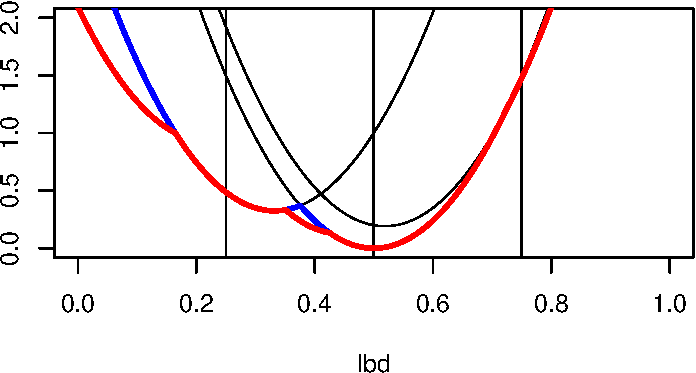
\includegraphics{minimization_files/figure-pdf/upperfig-1.pdf}

}

\caption{Piecewise Quadratic Upper Approximation}

\end{figure}%

\subsection{AM/GM Minorization}\label{propamgmmin}

Instead of approximating stress from above, we can also approximate it
from below.

\phantomsection\label{uplowenv}
\(\sigma\) is the upper envelop of an infinite number of quadratics.

\begin{proof}
By AM/GM

\begin{equation}
d_{ij}(X)\leq\min
\frac12\frac{1}{d_{ij}(Y)}\{d_{ij}^2(X)+d_{ij}^2(Y)\}
(\#eq:dasmin)
\end{equation}

Thus

\begin{equation}
\sigma(X)=\max_Y \left(1-\frac12\rho(Y)+\frac12\text{tr}\ X'(V-B(Y))X\right)
(\#eq:sigmax)
\end{equation}
\end{proof}

\begin{figure}[H]

{\centering 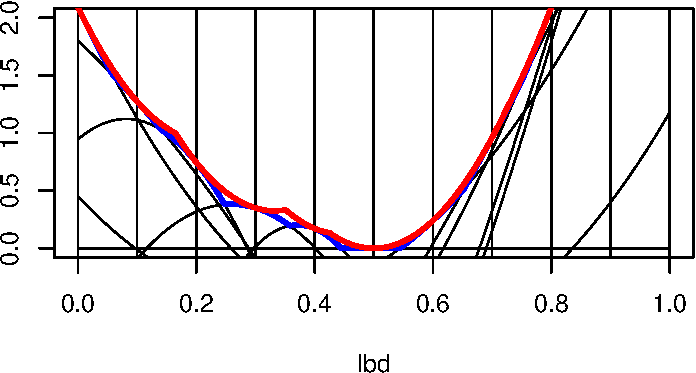
\includegraphics{minimization_files/figure-pdf/lowerfig-1.pdf}

}

\caption{Piecewise Quadratic Lower Approximation}

\end{figure}%

Again we illustrate this result using a finite number of quadratics. In
figure @ref(fig:lowerfig) we choose \(\lambda\) equal to 0, 0.1, 0.2,
0.3, 0.4, 0.5, 0.6, 0.7, 0.8, 0.9, 1. Although we now use 11 quadratics,
and thus force the envelop to be equal to the function at the 11 points
on the vertical lines in the plot, the approximation is poor. This seems
to be mainly because the convex-like function stress must be
approximated from below by quadratics which are often concave.

\subsection{Dualities}\label{dualities}

\begin{multline}
\min_X\sigma(X)=\min_Y \left(1 - \frac12\text{tr}\ Y'B(Y)V^+B(Y)Y\right)=\\1-\frac12\max_Y\text{tr}\ Y'B(Y)V^+B(Y)Y.
\end{multline}

Thus minimizing stress is equivalent to maximizing \(\eta^2(V^+B(X)X)\).

\[
\min_X\sigma(X)\geq\max_{B(Y)\lesssim V}(1-\rho(Y))
\]

By the minimax inequality
\(\min_X\sigma(X)=\min_X\max_Y\theta(X,Y)\geq\max_Y\min_X\theta(X,Y).\)
Now \(\min_X\theta(X,Y)\) is \(-\infty\), unless \(B(Y)\lesssim V\), in
which case \(\min_X\theta(X,Y)=0\). Thus \[
\max_Y\min_X\theta(X,Y)=\max_{B(Y)\lesssim V}(1-\rho(Y))=1-\min_{B(Y)\lesssim V}\ \rho(Y)
\]

\section{Smacof in Coefficient Space}\label{smacofcoef}

\section{Newton in MDS}\label{smacofnewton}

\subsection{Regions of Attraction}\label{attraction}

\begin{Shaded}
\begin{Highlighting}[]
\NormalTok{delta }\OtherTok{\textless{}{-}} \FunctionTok{as.matrix}\NormalTok{ (}\FunctionTok{dist}\NormalTok{ (}\FunctionTok{diag}\NormalTok{ (}\DecValTok{4}\NormalTok{)))}
\NormalTok{delta }\OtherTok{\textless{}{-}}\NormalTok{ delta }\SpecialCharTok{*} \FunctionTok{sqrt}\NormalTok{ (}\DecValTok{2} \SpecialCharTok{/} \FunctionTok{sum}\NormalTok{ (delta }\SpecialCharTok{\^{}} \DecValTok{2}\NormalTok{))}
\end{Highlighting}
\end{Shaded}

\subsubsection{Smacof}\label{attractsmacof}

We use the smacof() function from the code in the appendix with 100
different starting points of \(\theta\), equally spaced on the circle.
Figure @ref(fig:histsmacof) is a histogram of the number of smacof
iterations to convergence within 1e-15. In all cases smacof converges to
a local minimum in coefficient space, never to a saddle point. Figure
@ref(fig:pathsmacof) shows which local minima are reached from the
different starting points. This shows, more or less contrary to what
Trosset and Mathar (\citeproc{ref-trosset_mathar_97}{1997}) suggests,
that non-global minima can indeed be points of attraction for smacof
iterations.

\begin{figure}[H]

{\centering 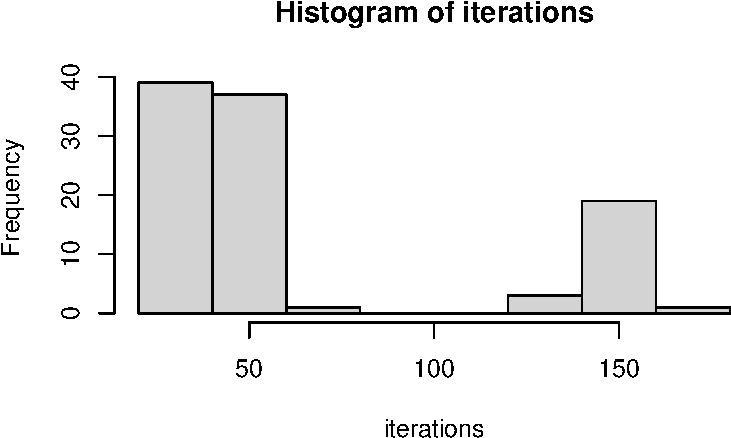
\includegraphics{minimization_files/figure-pdf/histsmacof-1.pdf}

}

\caption{Histogram Number of Smacof Iterations}

\end{figure}%

\begin{figure}[H]

{\centering 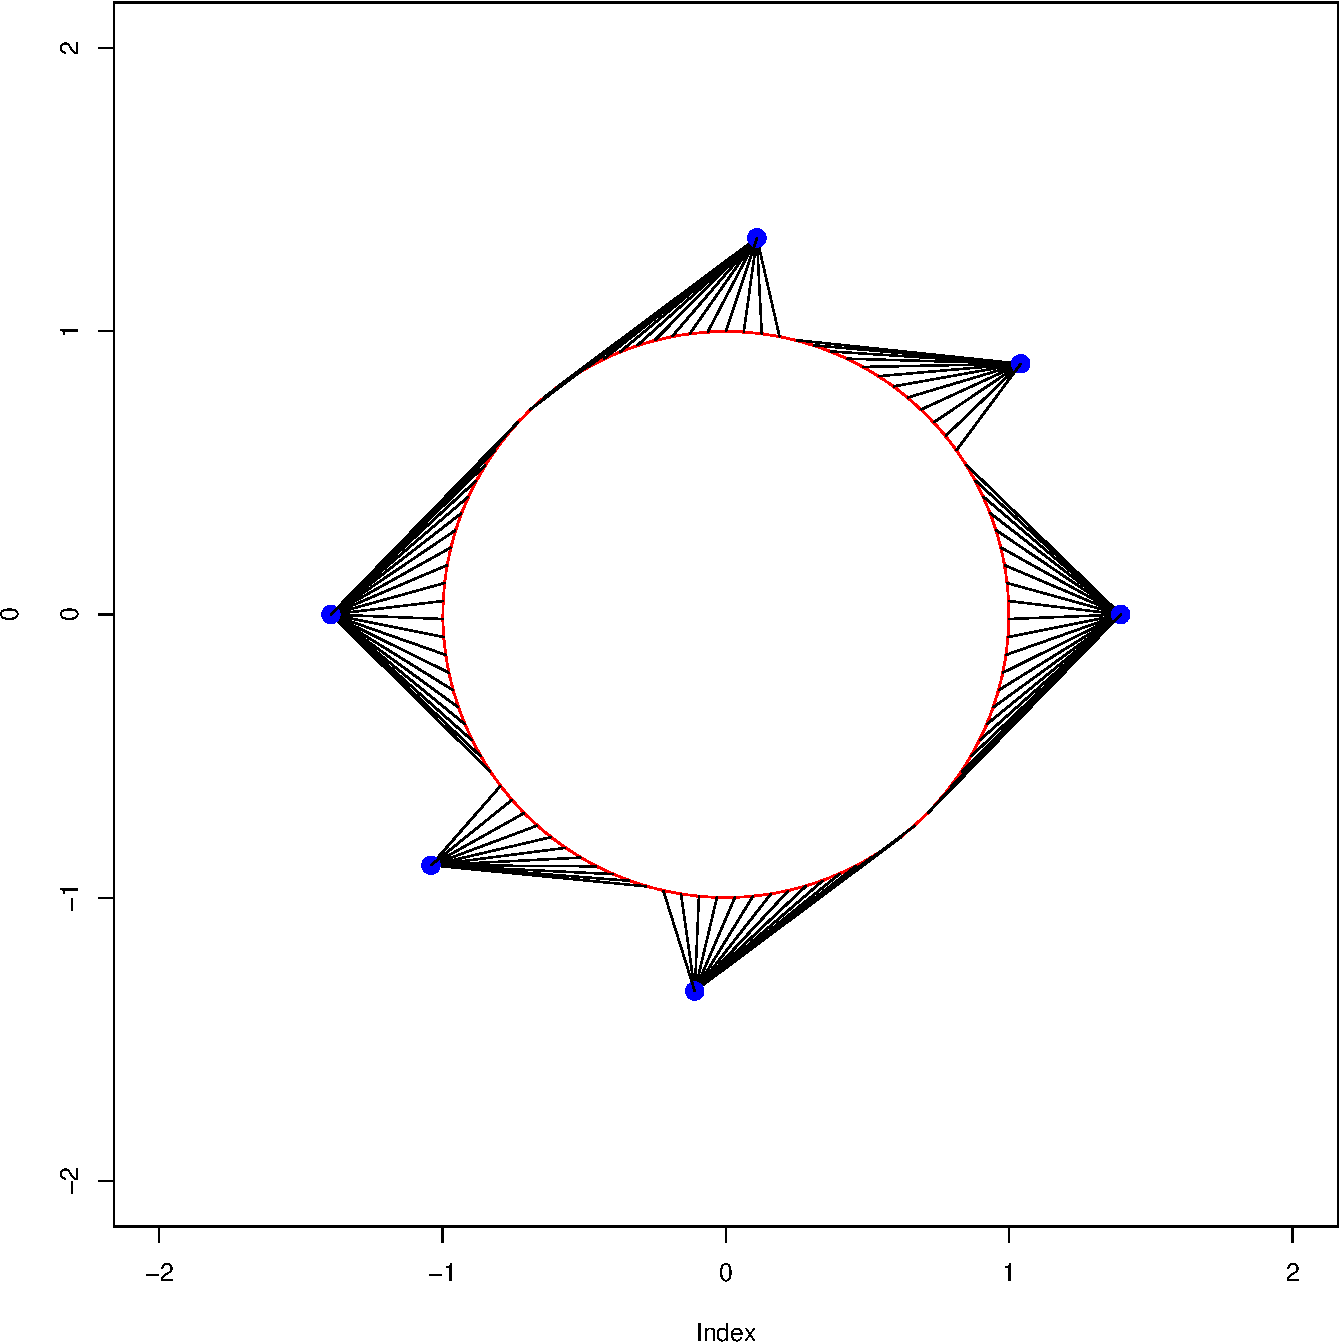
\includegraphics{minimization_files/figure-pdf/pathsmacof-1.pdf}

}

\caption{Path Endpoints of Smacof Iterations}

\end{figure}%

\subsubsection{Newton}\label{attractnewton}

We repeat the same exercise with Newton's method, which also converges
from all 100 starting points in our example. In higher dimensions we may
not be so lucky.

The histogram of iteration counts is in figure @ref(fig:histnewton). It
shows in this example that \texttt{smacof} needs about 10 times the
number of iterations that Newton needs. Because \texttt{smacof}
iterations are much less expensive than Newton ones, this does not
really say much about computing times. If we look at figure
@ref(fig:pathnewton) we see the problem with non-safeguarded Newton.
Although we have fast convergence from all 100 starting points, Newton
converges to a saddle point in 45 cases.

\begin{figure}[H]

{\centering 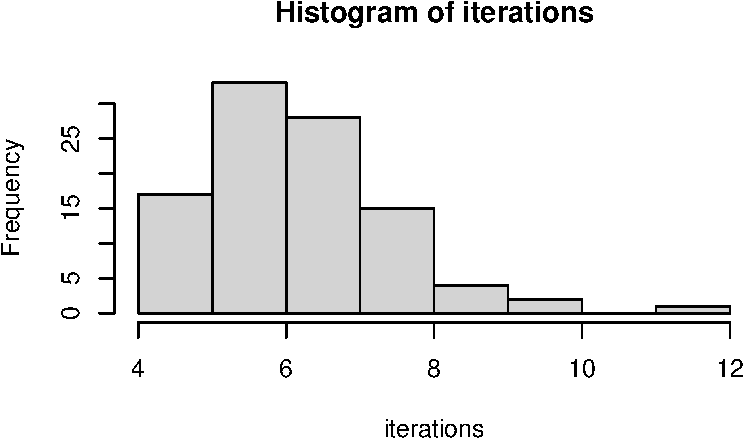
\includegraphics{minimization_files/figure-pdf/histnewton-1.pdf}

}

\caption{Histogram Number of Newton Iterations}

\end{figure}%

\begin{figure}[H]

{\centering 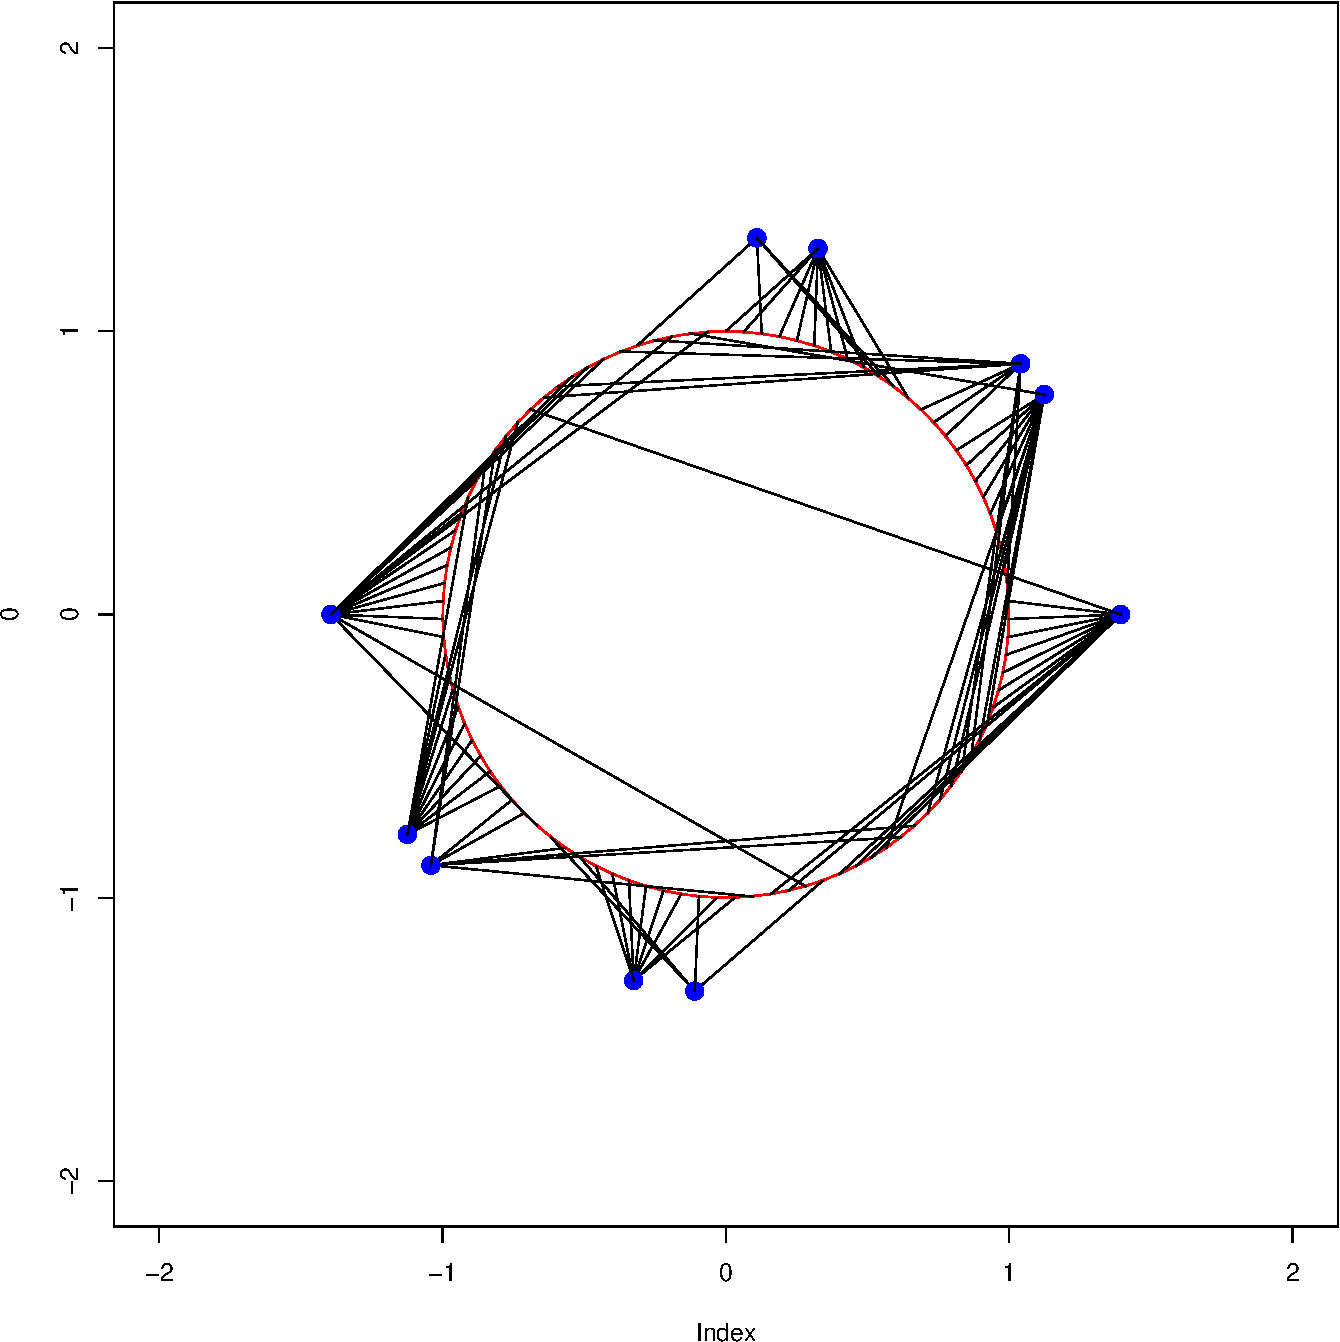
\includegraphics{minimization_files/figure-pdf/pathnewton-1.pdf}

}

\caption{Path Endpoints of Newton Iterations}

\end{figure}%

\section{Distance Smoothing}\label{propdistsmo}

In sections @ref(propconvex) and @ref(propstationary) we show the lack
of differentiability in basic MDS is not a serious problem in the actual
computation of local minima.

There is another rather straightforward way to circumvent the
differentiabily issue, which actually may have additional benefits. The
idea is to use an approximation of the Euclidean distance that is as
close as possible on the positive real axis, but smooth at zero. This
was first applied in unidimensional MDS by Pliner (Pliner
(\citeproc{ref-pliner_86}{1986}), Pliner
(\citeproc{ref-pliner_96}{1996})) and later taken up and generalized to
pMDS for arbitrary \(p\), and even for arbitrary Minkovski metrics, by
Groenen, Heiser, and Meulman
(\citeproc{ref-groenen_heiser_meulman_98}{1998}) and Groenen, Heiser,
and Meulman (\citeproc{ref-groenen_heiser_meulman_99}{1999}). They
coined the term \emph{distance smoothing} for this variation of the
\(\textrm{smacof}\) framework for MDS.

Pliner (\citeproc{ref-pliner_86}{1986}) uses a smooth approximation of
the sign function, while Groenen, Heiser, and Meulman
(\citeproc{ref-groenen_heiser_meulman_98}{1998}) borrow the smooth Huber
approximation of the absolute value function from robust regression. We
use another classical and efficient approximation
\(|x|\approx\sqrt{x^2+\epsilon^2}\) to the absolute value function, used
in image analysis, location analysis, and computational geometry (De
Leeuw (\citeproc{ref-deleeuw_E_18f}{2018b}), Ramirez et al.
(\citeproc{ref-ramirez_sanchez_kreinovich_argaez_14}{2014})). In our
context that becomes
\(d_{ij}(X)\approx d_{ij}(X,\epsilon):=\sqrt{d_{ij}^2(X)+\epsilon^2}\).
Note that on the non-negative reals \begin{equation}
\max(\epsilon,d_{ij}(X))\leq d_{ij}(X,\epsilon)\leq d_{ij}(X)+\epsilon.
(\#eq:smoothineq)
\end{equation} Figures @ref(fig:dfsmoother) and @ref(fig:ddsmoother)
show the absolute value function and its derivative are approximated for
\(\epsilon\) equal to 0, 0.01, 0.05, 0.1, 0.5.

\begin{figure}[H]

{\centering 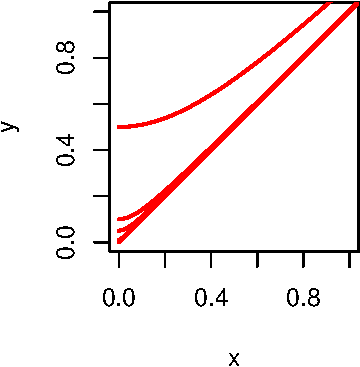
\includegraphics{minimization_files/figure-pdf/dfsmoother-1.pdf}

}

\caption{Function for Various Epsilon}

\end{figure}%

\begin{figure}[H]

{\centering 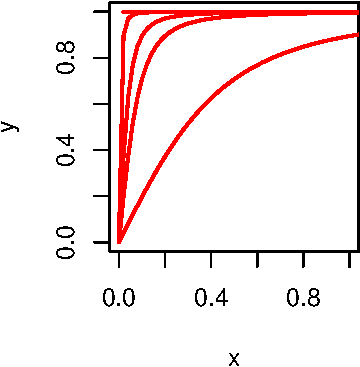
\includegraphics{minimization_files/figure-pdf/ddsmoother-1.pdf}

}

\caption{Derivative for Various Epsilon}

\end{figure}%

The distance smoother we use fits nicely into \(\textrm{smacof}\).
Define \(X_\epsilon:=\begin{bmatrix}X&\mid&\epsilon I\end{bmatrix}\).
Then \(d_{ij}(X_\epsilon)=\sqrt{d_{ij}^2(X)+\epsilon^2}\). Thus we can
define \begin{equation}
\sigma_\epsilon(X):=\sigma(X_\epsilon)=\mathop{\sum\sum}_{1\leq i<j\leq n}w_{ij}(\delta_{ij}- d_{ij}(X_\epsilon))^2,
(\#eq:sigmaepsilon)
\end{equation} with \(\rho_\epsilon\) and \(\eta^2_\epsilon\) defined in
the same way.

For a fixed \(\epsilon>0\) now \(d_{ij}(X_\epsilon)\), and thus stress,
is (infinitely many times) differentiable on all of
\(\mathbb{R}^{n\times p}\). Moreover \(d_{ij}(X,\epsilon)\) is convex in
\(X\) for fixed \(\epsilon\) and jointly convex in \(X\) and
\(\epsilon\), and as a consequence so are \(\rho_\epsilon\) and
\(\eta^2_\epsilon\).

\begin{figure}[H]

{\centering 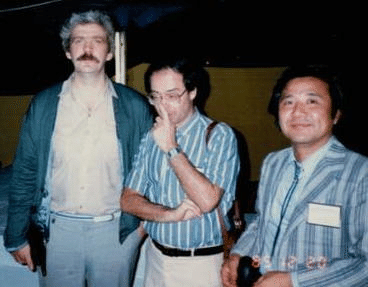
\includegraphics[width=0.6\textwidth,height=\textheight]{graphics/calcutta_12_85.png}

}

\caption{Jan de Leeuw, Gilbert Saporta, Yutaka Kanaka in Kolkata,
December 1985}

\end{figure}%

\bookmarksetup{startatroot}

\chapter{Nonmetric MDS}\label{nonmtrmds}

\section{Generalities}\label{generalities}

In non-metric MDS the dissimilarities are not a vector of known
non-negative numbers, but they are only known up to a transformation or
quantification. Ever since Kruskal (\citeproc{ref-kruskal_64a}{1964a})
the approach for dealing with this aspect of the MDS problem is to
define stress as a function of both \(X\) and \(\Delta\), and to
minimize \begin{equation}
\sigma(X,\Delta):=\mathop{\sum\sum}_{1\leq i<j\leq n}w_{ij}(\delta_{ij}-d_{ij}(X))^2
(\#eq:nmstress)
\end{equation} over both configurations \(X\) and feasible
\emph{disparities} (i.e.~transformed dissimilarities). The name
\emph{disparities} was coined, as far as I know, by Forrest Young and
used in our joint ALS work from the seventies (Takane, Young, and De
Leeuw (\citeproc{ref-takane_young_deleeuw_A_77}{1977})). Kruskal's name
for the transformed or quantified dissimilarities is
\emph{pseudo-distances}.

To work with a general notion of the feasability of a matrix of
disparities we use the notation \(\Delta\in\mathfrak{D}\). Typically,
although not necessarily, \(\mathfrak{D}\) is a convex set in disparity
space. In interval, polynomial, splinical, and ordinal MDS it usually is
a convex cone with apex at the origin. This implies that
\(0\in\mathfrak{D}\), and consequently that \begin{equation}
\min_{X\in\mathbb{R}^{n\times p}}\min_{\Delta\in\mathfrak{D}}=0,
(\#eq:nmtrivial)
\end{equation} with the minimum attained at \(X=0\) and \(\Delta=0\). Of
course this is a \emph{trivial solution}, which is completely
independent of the data. Thus we cannot formulate the NMDS problem as
the minimization of stress from equation @ref(eq:nmstress) over
unconstrained \(X\) and over \(\Delta\) in its cone. We need some way to
exclude either \(X=0\) or \(\Delta=0\), or both, from the feasible
solutions. This we can do either by normalization of the loss function,
or by using constraints that explicitly exclude one or both zero
solutions. The commonly used options will be discussed in section
@ref(nmdsnorm) of this chapter.

\subsection{Kruskal's Stress}\label{kruskals-stress-1}

\ldots{} we shall find ourselves doing arithmetic with dissimilarities.
This we must not do, because we are committed to using only the rank
ordering of the dissimilarities. (Kruskal
(\citeproc{ref-kruskal_64a}{1964a}), p 6-7)

section @ref(nmdsnorm)

\section{Single and Double Phase}\label{nmssingledouble}

The distinction between \emph{single phase} and \emph{double phase} NMDS
algorithms, introduced by Guttman (\citeproc{ref-guttman_68}{1968}), has
caused a great deal of confusion in the early stages of non-metric MDS
(say between 1960 and 1970).

\begin{quote}
This beguiling complex distinction has given rise to an almost endless
debate (among \textgreater{} Guttman, Kruskal, Lingoes, Roskam, and
Shepard -- for all permutations of five things taken two at a time) and
has caused anguish and despair (accompanied by an imprecation or two by
at least four of the five) extending over a three year period -- only
occasionally alleviated by evanescent flashes of partial insight
(Lingoes and Roskam (\citeproc{ref-lingoes_roskam_73}{1973}))
\end{quote}

I was an active, although late-arriving, participant in discussing, and
perhaps perpetuating, this confusion (De Leeuw
(\citeproc{ref-deleeuw_R_73g}{1973b})). For raking up this debate at
this late stage I was sternly spoken to by Jim Lingoes, who pointed me
to the discussion in Lingoes and Roskam
(\citeproc{ref-lingoes_roskam_73}{1973}).

\begin{quote}
I would hate to believe that after this heroic attempt on our part that
``we all'' would once more be engaged in a ``correspondence musical
chairs'' on these issues. (Lingoes in De Leeuw
(\citeproc{ref-deleeuw_R_73g}{1973b})).
\end{quote}

Nevertheless, even in later discussions of the distinction between
single-phase and double-phase (such as
(\citeproc{ref-roskam_79}{\textbf{roskam\_79?}})) I still get the
feeling that there are some unresolved misunderstandings. Thus I will
pay some more attention to the musical chairs here.

By the very definition of the minimum of a function we have the
mathematical truism \begin{equation}
\min_{(X,\Delta)\in\mathfrak{X}\otimes\mathfrak{D}}\sigma(X,\Delta)=
\min_{X\in\mathfrak{X}}\min_{\Delta\in\mathfrak{D}}\sigma(X,\Delta)=\min_{X\in\mathfrak{X}}\left\{\min_{\Delta\in\mathfrak{D}}\sigma(X,\Delta)\right\}=\min_{\Delta\in\mathfrak{D}}\left\{\min_{X\in\mathfrak{X}}\sigma(X,\Delta)\right\},
(\#eq:nmsminmin)
\end{equation} provided all minima exist. This is true no matter what
the subsets \(\mathfrak{X}\) of configuration space and \(\mathfrak{D}\)
of disparity space are.

\subsection{Double Phase}\label{double-phase}

In a \emph{double phase algorithm} we alternate the minimization of
stress over \(X\) and \(\Delta\). Thus \begin{align}
X^{(k+1)}&=\mathop{\text{argmin}}_{X\in\mathfrak{X}}\sigma(X,\Delta^{(k)}),(\#eq:nmsals1)\\
\Delta^{(k+1)}&=\mathop{\text{argmin}}_{\Delta\in\mathfrak{D}}\sigma(X^{(k+1)},\Delta).(\#eq:nmsals2).
\end{align} Thus double phase algorithms are \emph{alternating least
squares} or ALS algorithms. The designation ``alternating least
squares'' was first used, AFAIK, by De Leeuw
(\citeproc{ref-deleeuw_R_68d}{1968b}), and of course it was widely
disseminated by the series of ALS algorithms of Young, Takane, and De
Leeuw in the seventies (see F. W. Young (\citeproc{ref-young_81}{1981})
for a retrospective summary).

There are some possible variations in the ALS scheme. In equation
@ref(eq:nmsals1) we update \(X\) first, and then in equation
@ref(eq:nmsals1) we update \(\Delta\). That order can be reversed
without any essential changes. More importantly, we have to realize that
minimizing over \(X\) in equation @ref(eq:nmsals1) is a basic metric MDS
problem, which will generally take an infinite number of iterations for
an exact solution. This means we have to truncate the minimization, and
stop at some point. And, in addition, equation @ref(eq:nmsals1) implies
we have to find the global minimum over \(X\), which is generally
infeasible as well.Thus the ALS scheme as defined cannot really be
implemented.

We remedy this situations by switching from minimization in each substep
to a decrease, or, notationwise, from \(\text{argmin}\) to
\(\text{arglower}\). The resulting update sequence \begin{align}
X^{(k+1)}&=\mathop{\text{arglower}}_{X\in\mathfrak{X}}\sigma(X,\Delta^{(k)}),(\#eq:nmslte1)\\
\Delta^{(k+1)}&=\mathop{\text{arglower}}_{\Delta\in\mathfrak{D}}\sigma(X^{(k+1)},\Delta).(\#eq:nmslte2).
\end{align} is much more loosely defined than the previous one, because
arglower can be implemented in many different ways. More about that
later. But at least the new scheme can actually be implemented.

Algorithm \#ref(eq:nmslte1) and \#ref(eq:nmslte2) is still considered to
be ALS, but it is also firmly in the class of \emph{block relaxation}
algorithms. General block relaxation, which has alternating least
squares, coordinate relaxation, augmentation, EM, and majorization as
special cases, was used to describe many different data analysis
algorithms in De Leeuw (\citeproc{ref-deleeuw_C_94c}{1994}). As with
ALS, special cases of block relaxation have been around for a long time.

\subsection{Single Phase}\label{nmssinglephase}

From equation @ref(eq:nmsminmin) \begin{equation}
\min_{X\in\mathfrak{X}}\min_{\Delta\in\mathfrak{D}}\sigma(X,\Delta)=\min_{X\in\mathfrak{X}}\left\{\min_{\Delta\in\mathfrak{D}}\sigma(X,\Delta)\right\}.
(\#eq:nmsminsin)
\end{equation} So if we define \begin{equation}
\sigma_\star(X):=\min_{\Delta\in\mathfrak{D}}\sigma(X,\Delta),
(\#eq:nmssingle)
\end{equation} the NMDS problem is to minimize \(\sigma_\star\) from
@ref(eq:nmssingle) over \(X\). Note there is a \(\sigma\) defined by
equation @ref(eq:nmstress) on \(\mathfrak{X}\otimes\mathfrak{D}\), and a
\(\sigma_\star\), defined by equation @ref(eq:nmssingle), which is a
function only of \(X\). It is sometimes said that that \(\Delta\) is
\emph{projected} when going from @ref(eq:nmstress) to
@ref(eq:nmssingle), or that \(\sigma_\star\) is a \emph{marginal}
function.

Once more with feeling. The two-phase \(\sigma\) is a function of two
matrix variables \(X\) and \(\Delta\), the one-phase \(\sigma_\star\)is
a function of the single matrix variable \(X\). To make this even more
clear we can write \(\sigma_\star(X)=\sigma(X,\Delta(X))\), where
\begin{equation}
\Delta(X):=\mathop{\text{argmin}}_{\Delta\in\mathfrak{D}}\sigma(X,\Delta).
(\#eq:nmsdeltasingle)
\end{equation}

Of course by projecting out \(X\) instead of \(\Delta\) we could also
have defined a loss function which is a function of \(\Delta\) only, but
typically we do not use the alternative projection because it is
complicated and heavily nonlinear. Projecting out \(X\) is, in fact,
solving a standard basic MDS problem. Projecting out \(\Delta\) is
usually much simpler. In most applications \(\mathfrak{D}\) is convex,
so computing \(\Delta(X)\) is computing the projection on a convex set,
and projections on convex sets always exist and are unique and
continuous.

As an aside, projection creates a function of one variable out of a
function of two variables. The inverse of projection is called
\emph{augmentation}, which starts with a function \(f\) of one variable
on \(\mathfrak{X}\) and tries to find a function of two variables \(g\)
on \(\mathfrak{X}\otimes\mathfrak{Y}\) such that
\(f(x)=\min_{y\in\mathfrak{Y}} g(x,y)\). If we have found such a \(g\)
then we can minimize \(f\) over \(\mathfrak{X}\) by minimizing \(g\)
over \(\mathfrak{X}\otimes\mathfrak{Y}\), for example by block
relaxation (De Leeuw (\citeproc{ref-deleeuw_C_94c}{1994})).

One reason there was some confusion, and some disagreement between
Kruskal and Guttman, was a result on differentiation of the minimum
function, which was not known in the psychometric community at the time.
Guttman thought that \(\sigma_\star\) was not differentiable at \(X\),
because \(\Delta\) from @ref(eq:nmsdeltasingle) is a step function.
Kruskal proved in Kruskal (\citeproc{ref-kruskal_71}{1971}) that
\(\sigma_\star\) is differentiable, and saw that the result is basically
one in convex analysis, not in classical linear analysis. The result
follows easily from directional differentiability in Danskin's theorem
(Danskin (\citeproc{ref-danskin_67}{1967})) or from the minimax theorems
of, for example, Demyanov and Malozemov
(\citeproc{ref-demyanov_malozemov_90}{1990}), using the fact that the
projection is unique. More directly, deleeuw\_R\_73g refers to
discussion on page 255 of Rockafellar
(\citeproc{ref-rockafellar_70}{1970}), following his corollary 26.3.2.
We will go into more detail about differentiability, and the differences
between Kruskal's and Guttman's loss functions, in the next chapter
@ref(chapordinal). For now it suffices to note that \begin{equation}
\mathcal{D}\sigma_\star(X)=\mathcal{D}_1\sigma(X,\Delta(X)),
(\#eq:nmsdanskin)
\end{equation} or, in words, that the derivative of \(\sigma_\star\) at
\(X\) is the partial derivative of \(\sigma\) at \((X,\Delta(X))\).

\section{Affine NMDS}\label{affine-nmds}

Basic MDS can now be interpreted as the special case of NMDS in which
\(\mathfrak{D}=\{\Delta\}\) is a singleton, a set with only one element.
Thus \(0\not\in\mathfrak{D}\) and we do not have to worry about trivial
zero solutions for \(X\).

This extends to basic MDS with missing data. We have so far dealt with
missing data by setting the corresponding \(w_{ij}\) equal to zero. But
for the non-missing part we still have fixed numbers in \(\Delta\), and
thus again \(0\not\in\mathfrak{D}\) (unless all dissimilarities are
missing). In a sense missing data are our first example of non-metric
MDS, because \(\mathfrak{D}\) can also be defined as the set
\begin{equation}
\mathfrak{D}=
\left\{\Delta\mid\Delta_0+\mathop{\sum\sum}_{1\leq i<j\leq n}\{\alpha_{ij}(E_{ij}+E_{ji})\mid \delta_{ij}\text{ is missing}\}\right\},
(\#eq:nmsmissing)
\end{equation} where the \(E_{ij}\) are the unit matrices defined in
section @ref(\#propmatrix) and \(\Delta_0\) is the non-missing part
(which has zeroes for the missing elements).

Single/double phase

Another example in which \(0\not\in\mathfrak{D}\) is the additive
constant problem, which we will discuss in detail in section
@ref(intadditive). Here \(\mathfrak{D}\) is the set of all hollow and
symmetric matrices of the form \(\Delta+\alpha(E-I)\), where the
dissimilarities in \(\Delta_0\) are known real numbers and where
\(\alpha\) is the unknown additive constant.

Affine MDS problems also have single phase and double phase algorithms.
For missing data single phase stress is \begin{equation}
\sigma_\star(X)=\min_{\Delta\in\mathfrak{D}}\ \mathop{\sum\sum}_{1\leq i<j\leq n}w_{ij}(\delta_{ij}-d_{ij}(X))^2=\mathop{\sum\sum}_{1\leq i<j\leq n}\tilde w_{ij}(\delta_{ij}-d_{ij}(X))^2,
(\#eq:nmssinglemis)
\end{equation} where \(\tilde w_{ij}=0\) if \(\delta_{ij}\) is missing,
and \(\tilde w_{ij}=w_{ij}\) otherwise. In this case
\(\sigma_\star(X)=\sigma(X)\), the sigma of basic MDS with zero weights
for missing data.

For the additive constant problem single phase stress is
\begin{equation}
\sigma_\star(X)=\min_{\alpha}\mathop{\sum\sum}_{1\leq i<j\leq n}w_{ij}(\delta_{ij}+\alpha-d_{ij}(X))^2=\mathop{\sum\sum}_{1\leq i<j\leq n} w_{ij}(\delta_{ij}-d_{ij}(X))^2-(\overline\delta-\overline d(X))^2\mathop{\sum\sum}_{1\leq i<j\leq n}w_{ij},
(\#eq:nmssingleadd)
\end{equation} where \(\overline\delta\) and \(\overline d(X)\) are the
weighted means of the dissimilarities and distances.

\section{Conic NMDS}\label{nmdsconic}

\subsection{Normalization}\label{nmdsnorm}

In ``wide-sense'' non-metric MDS \(\mathfrak{D}\) can be any set of
hollow, non-negative and symmetric matrices. In ``narrow-sense''
non-metric MDS \(\mathfrak{D}\) is defined by homogeneous linear
inequality constraints of the form \(\delta_{ij}\leq\delta_{kl}\) (in
addition to hollow, non-negative, and symmetric). These constraints,
taken together, define a polyhedral convex cone in disparity space. This
just means that if \(\Delta_1\) and \(\Delta_2\) are in \(\mathfrak{D}\)
then so is \(\alpha\Delta_1+\beta\Delta_2\) for all non-negative
\(\alpha\) and \(\beta\).

The disparities define a cone, and thus \(0\in\mathfrak{D}\). This
implies that always
\(\min_X\min_{\Delta\in\mathfrak{D}}\sigma(X,\Delta)=0,\) independently
of the data. This is our first example of a \emph{trivial solution},
which have plagued non-metric scaling from the start. Note that
\(\mathfrak{D}\) for missing data and for the additive constant are not
convex cones, and do not contain the zero matrix.

In our versions of \emph{non-metric} MDS we actually require that the
transformed dissimilarities satisfy \(\eta_\delta=1\), so that formula
@ref(eq:expand) is still valid. We call this \textbf{explicit
normalization of the dissimilarities}.

To explain the different forms of normalization of stress that are
needed whenever \(\mathfrak{D}\) is a cone we look at some general
properties of least squares loss functions. More details are in Kruskal
and Carroll (\citeproc{ref-kruskal_carroll_69}{1969}) and in De Leeuw
(\citeproc{ref-deleeuw_U_75a}{1975a}), De Leeuw
(\citeproc{ref-deleeuw_E_19d}{2019}).

Suppose \(K\) and \(L\) are cones in \(\mathbb{R}^n\), nor necessarily
convex. Our problem is to minimize \(\|x-y\|^2\) over both \(x\in K\)
and \(y\in L\). Here \(\|x\|^2=x'Wx\) for some positive definite \(W\).
In the MDS context, for \(x\) think disparities, for \(y\) think
distances.

Of course minimizing \(\|x-y\|^2\) is too easy, because \(x=y=0\) is the
(trivial, and useless) solution. So we need some form of normalization.
We distinguish six different ones.

\begin{enumerate}
\def\labelenumi{\arabic{enumi}.}
\item
  implicit x-normalization \[
  \min_{x\in K}\min_{y\in L}\frac{\|x-y\|^2}{\|x\|^2}
  \]
\item
  implicit y-normalization \[
  \min_{x\in K}\min_{y\in L}\frac{\|x-y\|^2}{\|y\|^2}
  \]
\item
  implicit xy-normalization \[
  \min_{x\in K}\min_{y\in L}\frac{\|x-y\|^2}{\|x\|^2\|y\|^2}
  \]
\item
  explicit x-normalization \[
  \min_{x\in K\cap S}\min_{y\in L}\|x-y\|^2
  \]
\item
  explicit y-normalization \[
  \min_{x\in K}\min_{y\in L\cap S}\|x-y\|^2
  \]
\item
  explicit xy-normalization \[
  \min_{x\in K\cap S}\min_{y\in L\cap S}\|x-y\|^2
  \] If we use a positive definite \(W\) to define our inner products
  and norms, then implicit normalization of \(x\) means \[
  \min_{x\in X}\min_{y\in Y}\frac{(x-y)'W(x-y)}{x'Wx}.
  \] Let \(\mathcal{S}_x\) and \(\mathcal{S}_y\) be the ellipsoids of
  all \(x\) with \(x'Wx=1\) and of all \(y\) with \(y'Wy=1\). Then our
  implicit normalization problem is equivalent to \[
  \min_{\alpha\geq 0}\min_{\beta\geq 0}\min_{x\in X\cap\mathcal{S}_x}\min_{y\in Y\cap\mathcal{S}_y}\frac{(\alpha x-\beta y)'W(\alpha x-\beta y)}{\alpha^2 x'Wx}=\\\min_{x\in X\cap\mathcal{S}_x}\min_{y\in Y\cap\mathcal{S}_y}\min_{\alpha\geq 0}\min_{\beta\geq 0}\frac{\alpha^2+\beta^2-2\alpha\beta x'Wy}{\alpha^2}=\\
  \min_{x\in X\cap\mathcal{S}_x}\min_{y\in Y\cap\mathcal{S}_y}\ \{1-(x'Wy)^2\}.
  \] Thus implicit normalization of \(x\) means maximizing \((x'Wy)^2\)
  over \(x\in X\cap\mathcal{S}_x\) and \(y\in Y\cap\mathcal{S}_y.\)
\end{enumerate}

In the same way implicit normalization of \(y\) minimizes \[
\min_{x\in X}\min_{y\in Y}\frac{(x-y)'W(x-y)}{y'Wy},
\] and in the same way it also leads to maximization of \((x'Wy)^2\)
over \(x\in X\cap\mathcal{S}_x\) and \(y\in Y\cap\mathcal{S}_y.\) In
terms of normalized stress it does not matter if we use the distances or
the dissimilarities in the denominator for implicit normalization.

In explicit normalization of \(x\) we solve \[
\min_{x\in X\cap\mathcal{S}_x}\min_{y\in Y}\ \{1+y'Wy-2y'Wx\}=\\
\min_{\beta\geq 0}\min_{x\in X\cap\mathcal{S}_x}\min_{y\in Y\cap\mathcal{S}_y}\{1+\beta^2-2\beta x'Wy\}
=\\\min_{x\in X\cap\mathcal{S}_x}\min_{y\in Y\cap\mathcal{S}_y}\ \{1-(x'Wy)^2\},
\] and the same thing is true for explicit normalization of \(y\), which
is \[
\min_{x\in X}\min_{y\in Y\cap\mathcal{S}_y}\ \{1+x'Wx-2y'Wx\}
\] So, again, it does not matter which one of the four normalizations we
use, explicit/implicit on disparities/distances, the solutions will all
be proportional to each other, i.e.~the same except for scale factors.

\subsection{Normalized Cone
Regression}\label{normalized-cone-regression}

\subsection{Hard Squeeze and Soft
Squeeze}\label{hard-squeeze-and-soft-squeeze}

\subsection{Inner Iterations}\label{inner-iterations}

\subsection{Stress-1 and Stress-2}\label{stress-1-and-stress-2}

In his original papers Kruskal (\citeproc{ref-kruskal_64a}{1964a}) and
Kruskal (\citeproc{ref-kruskal_64b}{1964b}) defined two versions of
normalized stress for nonmetric MDS. The first was \[
\sigma_{JBK1}(X):=\sqrt{\frac{\mathop{\sum\sum}_{1\leq i<j\leq n}(\hat d_{ij}-d_{ij}(X))^2}{\mathop{\sum\sum}_{1\leq i<j\leq n}d_{ij}^2(X)}}
\] \[
\sigma_{JBK2}(X):=\sqrt{\frac{\mathop{\sum\sum}_{1\leq i<j\leq n}(\hat d_{ij}-d_{ij}(X))^2}{\mathop{\sum\sum}_{1\leq i<j\leq n}(d_{ij}(X)-\overline{d}(X))^2}}
\] where the \(hat d_{ij}\) (the d-hats) are the pseudo-distances
obtained by projecting the \(d_{ij}(X)\) on the isocone defined by the
order of the dissimilarities, i.e.~by monotone regression (see section
@ref(mathsimpiso)). The \(\overline{d}(X)\) in the denominator of
\(\sigma_{JBK2}\) is the average of the distances.

There are some differences with the definition of stress in this book.

\begin{enumerate}
\def\labelenumi{\arabic{enumi}.}
\tightlist
\item
  We do not use the square root.
\item
  We use explicit and not implicit normalization.
\item
  In NMDS we think of stress as a function of both \(X\) and \(\Delta\),
  not of \(X\) only (see section @ref(nmdskruskal)).
\end{enumerate}

\bookmarksetup{startatroot}

\chapter{Interval MDS}\label{intinterval}

intro: additive vs interval basic vs ratio

\section{The Additive Constant}\label{intadditive}

\subsection{Early}\label{early}

In the early history of MDS dissimilarities were computed from
comparative judgments in the Thurstonian tradition.

triads paired comparisons etc positive orthant

These early techniques only gave numbers on an interval scale,
i.e.~dissimilarities known only up to a linear transformation. In order
to get positive dissimilarities a rational origin needed to be found in
some way. This is the \emph{additive constant problem}. It can be seen
as the first example of nonmetric MDS, in which we have only partially
known dissimilarities (up to an additive constant).

\begin{align}
\begin{split}
(\delta_{ij}+\alpha)&\approx d_{ij}(X),\\
\delta_{ij}&\approx d_{ij}(X)+\alpha.
\end{split}
(\#eq:twoadd)
\end{align}

The additive constant techniques were more important in the fifties and
sixties than they are these days, because they have largely been
replaced by iterative nonmetric MDS techniques.

An early algorithm to fit the additive constant based on Schoenberg's
theorem was given by Messick and Abelson
(\citeproc{ref-messick_abelson_56}{1956}). Ii was Torgerson based,
i.e.~it used the eigenvalues of \(\tau(\Delta^{(2)})\). It was a
somewhat hopeful iterative technique, without a convergence proof,
designed to make the sum of the \(n-p\) smallest eigenvalues equal to
zero. This is of course only a necessary condition for best
approximation, not a sufficient one.

In addition, the Messick-Abelson algorithm sometimes yielded solutionsin
which the Torgerson transform of the squared dissimilarities had
negative eigenvalues, which could even be quite large. That is also
somewhat of a problem.

\subsection{Cooper}\label{cooper}

Consequently Cooper (\citeproc{ref-cooper_72}{1972}) proposed an
alternative additive constant algorithm, taking his clue from the work
of Kruskal.

The solution was to redefine stress as a function of both the
configuration and the additive constant. Thus

\begin{equation}
\sigma(X,\alpha):=\mathop{\sum\sum}_{1\leq j<i\leq n}w_{ij}(\delta_{ij}+\alpha-d_{ij}(X))^2,
(\#eq:nmcooper1)
\end{equation}

and we minimize this stress over both \(X\) and \(\alpha\).

Double phase (ALS)

\(\delta_{ij}+\alpha\geq 0\)

Single Phase (Cooper)

\begin{equation}
\sigma(X):=\min_\alpha\mathop{\sum\sum}_{1\leq j<i\leq n}w_{ij}(\delta_{ij}+\alpha-d_{ij}(X))^2,
(\#eq:nmcooper2)
\end{equation}

\section{Algebra}\label{exactad}

The additive constant problem is to find \(X\in\mathbb{R}^{n\times p}\)
and \(\alpha\) such that \(\Delta+\alpha(E-I)\approx D(X)\). In this
section we look for all \(\alpha\) such that \(\Delta+\alpha(E-I)\) is
Euclidean, i.e. such that there is a configuration \(X\) with
\(\Delta+\alpha(E-I)=D(X)\). This is a one-parameter generalization of
Schoenberg's theorem.

It makes sense to require \(\alpha\geq 0\), because a negative
\(\alpha\) would more appropriately be called a subtractive constant.
Also, we may want to make sure that the off-diagonal elements of
\(\Delta+\alpha(E-I)\) are non-negative, i.e.~that
\(\alpha\geq-\delta_{ij}\) for all \(i>j\). Note that if we allow a
negative \(\alpha\) then if all off-diagonal \(\delta_{ij}\) are equal,
say to \(\delta>0\), we have the trivial solution \(\alpha=-\delta\) and
\(X=0\).

\subsection{Existence}\label{existence}

We start with a simple construction.

\begin{Shaded}
\begin{Highlighting}[]
\NormalTok{For all $\textbackslash{}Delta$ there is an $\textbackslash{}alpha\_0\textbackslash{}geq 0$ such that for all $\textbackslash{}alpha\textbackslash{}geq\textbackslash{}alpha\_0$ we have $\textbackslash{}Delta+\textbackslash{}alpha(E{-}I))$ Euclidean of dimension $r\textbackslash{}leq n{-}1$.}
\end{Highlighting}
\end{Shaded}

\begin{proof}
We have, using \(\Delta\times(E-I)=\Delta\) and
\((E-I)\times(E-I)=E-I\),

\begin{equation}
  \tau((\Delta+\alpha(E-I))\times(\Delta+\alpha(E-I)))=
  \tau(\Delta\times\Delta)+2\alpha\tau(\Delta)+\frac12\alpha^2J.
(\#eq:tau1)
\end{equation}

Thus each off-diagonal element is a concave quadratic in \(\alpha\),
which is negative for \(\alpha\) big enough. Choose \(\alpha_0\geq 0\)
to make all off-diagonal elements negative (and all dissimilarities
non-negative). A doubly-centered matrix with all off-diagonal elements
negative is positive semi-definite of rank \(n-1\) (Taussky
(\citeproc{ref-taussky_49}{1949})).
\end{proof}

Note that by the same argument we can also find a negative \(\alpha_0\)
that makes all off-diagonal elements negative and thus
\(\Delta+\alpha(E-I))\) is again Euclidean of dimension \(r\leq n-1\).
But this \(\alpha_0\) will usually result in negative dissimilarities.

Theorem @ref(thm:nmn1) can be sharpened for non-Euclidean \(\Delta\).
Define the following function of \(\alpha\):

\begin{equation}
\lambda_\star(\alpha):=\min_{x'x=1, x'e=0}x'\{\tau(\Delta\times\Delta)+2\alpha\tau(\Delta)+\frac12\alpha^2J\}x.
(\#eq:lambdas)
\end{equation}

This is the smallest non-trivial eigenvalue of the Torgerson transform
in @ref(eq:tau1). The matrix \(\Delta+\alpha(E-I)\) is Euclidean if and
only if \(\lambda_\star(\alpha)\geq 0\). Note that \(\lambda_\star\) is
continuous, by a simple special case of the Maximum Theorem (Berge
(\citeproc{ref-berge_63}{1963}), Chapter VI, section 3), and coercive,
i.e.~\(\lambda_\star(\alpha)\rightarrow +\infty\) if
\(|\alpha|\rightarrow +\infty\).

\begin{Shaded}
\begin{Highlighting}[]
\NormalTok{For all non{-}Euclidean $\textbackslash{}Delta$ there is an $\textbackslash{}alpha\_1\textgreater{}0$ such that for all $\textbackslash{}alpha\textbackslash{}geq\textbackslash{}alpha\_1$ we have that $\textbackslash{}Delta+\textbackslash{}alpha(E{-}I))$ Euclidean of dimension $r\textbackslash{}leq n{-}2$.}
\end{Highlighting}
\end{Shaded}

\begin{proof}
Because \(\Delta\) is non-Euclidean we have \(\lambda_\star(0)<0\). By
the construction in theorem @ref(thm:nmn1) there is an \(\alpha_0\) such
that \(\lambda_\star(\alpha)>0\) for all \(\alpha>\alpha_0\). By the
Maximum Theorem the function \(\lambda_\star\) is continuous, and thus,
by Bolzano's theorem, there is an \(\alpha_1\) between \(0\) and
\(\alpha_0\) such that \(\lambda_\star(\alpha_1)=0\). If there is more
than one zero between \(0\) and \(\alpha_0\) we take the largest one as
\(\alpha_1\).
\end{proof}

The problem with extending theorem @ref(thm:nmn2) to Euclidean
\(\Delta\) is that the equation \(\lambda_\star(\alpha)=0\) may have
only negative roots, or, even more seriously, no roots at all. This may
not be too important from the practical point of view, because observed
dissimilarities will usually not be exactly Euclidean. Nevertheless I
feel compelled to address it.

\begin{Shaded}
\begin{Highlighting}[]
\NormalTok{If $\textbackslash{}Delta$ is Euclidean then $\textbackslash{}lambda\_\textbackslash{}star(\textbackslash{}alpha)$ is non{-}negative and non{-}decreasing on $[0,+\textbackslash{}infty)$.}
\end{Highlighting}
\end{Shaded}

\begin{proof}
If \(\Delta\) is Euclidean, then \(\sqrt{\Delta}\), which is short for
the matrix with the square roots of the dissimilarities, is Euclidean as
well. This follows because the square root is a Schoenberg transform
(Schoenberg (\citeproc{ref-schoenberg_37}{1937}), Bavaud
(\citeproc{ref-bavaud_11}{2011})), and it implies that
\(\tau(\Delta)=\tau(\sqrt{\Delta}\times\sqrt{\Delta})\) is positive
semi-definite. Thus the matrix @ref(eq:tau1) is positive semi-definite
for all \(\alpha\geq 0\). By Danskin's Theorem the one-sided directional
derivative of \(\lambda_\star\) at \(\alpha\) is
\(2x(\alpha)'\tau(\Delta)x(\alpha)+\alpha\), where \(x(\alpha)\) is one
of the minimizing eigenvectors. Because the one-sided derivative is
non-negative, the function is non-decreasing (in fact increasing if
\(\alpha>0\)).
\end{proof}

Of course \(\lambda_\star(\alpha)=0\) can still have negative solutions,
and in particular it will have at least one negative solution if
\(\lambda_\star(\alpha)\leq 0\) for any \(\alpha\). There can even be
negative solutions with \(\Delta+\alpha(E-I)\) non-negative.

\subsection{Solution}\label{solution}

The solutions of \(\lambda_\star(\alpha)=0\) can be computed and studied
in more detail, using results first presented in the psychometric
literature by Cailliez (\citeproc{ref-cailliez_83}{1983}). We reproduce
his analysis here, with a somewhat different discussion that relies more
on existing mathematical results.

In order to find the smallest \(\alpha\) we solve the quadratic
eigenvalue problem (Tisseur and Meerbergen
(\citeproc{ref-tisseur_meerbergen_01}{2001})). WHY ??

\begin{equation}
\{\tau(\Delta\times\Delta)+2\alpha\tau(\Delta)+\frac12\alpha^2J\}y=0.
(\#eq:qep1)
\end{equation}

A solution \((y,\alpha)\) of \#ref(eq:qep1) is an eigen pair, in which
\(y\) is an eigenvector, and \(\alpha\) the corresponding eigenvalue.
The trivial solution \(y=e\) satisfies \#ref(eq:qep1) for any
\(\alpha\). We are not really interested in the non-trivial eigenvectors
here, but we will look at the relationship between the eigenvalues and
the solutions of \(\lambda_\star(\alpha)=0\).

The eigenvalues can be complex, in which case they do not interest us.
If \(\alpha\) is a non-trivial real eigenvalue, then the rank of the
Torgerson transform of the matrix in \#ref(eq:qep1) is \(n-2\), but

To get rid of the annoying trivial solution \(y=e\) we use a square
orthonormal matrix whose first column is proportional to \(e\). Suppose
\(L\) contains the remaining \(n-1\) columns. Now solve

\begin{equation}
\{L'\tau(\Delta\times\Delta)L+2\alpha L'\tau(\Delta)L+\frac12\alpha^2I\}y=0.
(\#eq:qep2)
\end{equation}

Note that the determinant of the polynomial matrix in @ref(eq:qep2) is a
polynomial of degree \(2(n-1)\) in \(\alpha\), which has \(2(n-1)\) real
or complex roots.

The next step is linearization (Gohberg, Lancaster, and Rodman
(\citeproc{ref-gohberg_lancaster_rodman_09}{2009}), chapter 1), which
means finding a linear or generalized linear eigen problem with the same
roots as @ref(eq:qep2). In our case this is the eigenvalue problem for
the matrix

\begin{equation}
\begin{bmatrix}
\hfill 0&\hfill I\\
-2L'\tau(\Delta\times\Delta)L&-4L'\tau(\Delta)L
\end{bmatrix}
(\#eq:qep3)
\end{equation}

\subsection{Examples}\label{examples}

\subsubsection{Small Example}\label{small-example}

Here is a small artificial dissimilarity matrix.

\begin{verbatim}
  1  2  3  4 
1 +0 +1 +2 +5
2 +1 +0 +4 +2
3 +2 +4 +0 +1
4 +5 +2 +1 +0
\end{verbatim}

It is constructed such that \(\delta_{14}>\delta_{12}+\delta_{24}\) and
that \(\delta_{23}>\delta_{21}+\delta_{13}\). Because the triangle
inequality is violated the dissimilarities are not distances in any
metric space, and certainly not in a Euclidean one. Because the minimum
dissimilarity is \(+1\), we require that the additive constant
\(\alpha\) is at least \(-1\).

The R function treq() in appendix @ref(apcodeclass) finds the smallest
additive constant such that all triangle inequalities are satisfied. For
this example it is \(\alpha=2\).

The Torgerson transform of \(\Delta\times\Delta\) is

\begin{verbatim}
  1      2      3      4     
1 +4.312 +2.688 +1.188 -8.188
2 +2.688 +2.062 -5.938 +1.188
3 +1.188 -5.938 +2.062 +2.688
4 -8.188 +1.188 +2.688 +4.312
\end{verbatim}

with eigenvalues

\begin{verbatim}
[1] +12.954 +7.546  +0.000  -7.750 
\end{verbatim}

The smallest eigenvalue -7.75 is appropriately negative, and theorem
@ref(thm:nmn2) shows that \(\Delta\times\Delta+7.75(E-I)\) are squared
distances between four points in the plane.

The upper bound for the smallest \(\alpha\) from theorem @ref(thm:nmn1),
computed by the R function acbound(), is 9.309475.

It is useful to look at a graphical representation of the minimum
non-trivial eigenvalue of
\(\tau((\Delta+\alpha(E-I))\times(\Delta+\alpha(E-I)))\) as a function
of \(\alpha\). The R function aceval() generates the data for the plot.

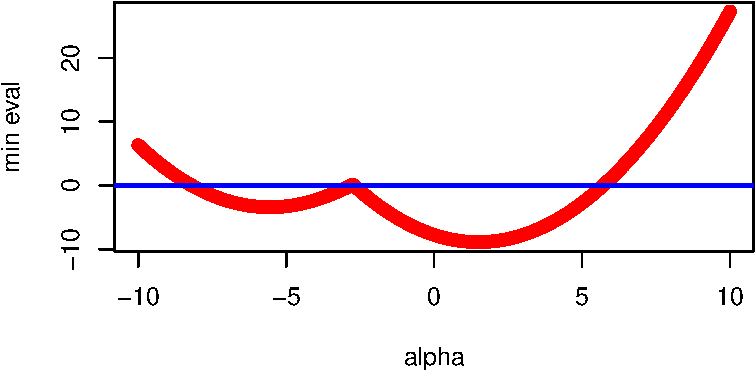
\includegraphics{interval_files/figure-pdf/acplot-1.pdf}

We see that the minimum non-trivial eigenvalue is a continuous function
of \(\alpha\),but one which certainly is not convex or concave or
differentiable. The graph crosses the horizontal axes near -8, -3, and
+6.

To make this precise we apply the theory of section xxx. The R function
acqep() finds the six non-trivial eigenvalues

\begin{verbatim}
[1] -8.192582+0.000000i  5.713075+0.000000i -3.500000+2.179449i
[4] -3.500000-2.179449i -2.807418+0.000000i -2.713075+0.000000i
\end{verbatim}

Two of the eigenvalues are complex conjugates, four are real. Of the
real eigenvalues three are negative, and only one is positive, equal to
+5.713. The table above gives the eigenvalues of the Torgerson
transform, using all four real eigenvalues for \(\alpha\). The three
negative ones do result in a positive semi-definite matrix with rank
equal to \(n-2\), but they also create negative dissimilarities.

\begin{verbatim}
 -8.193  ******  +38.098 +13.885  +0.000  +0.000 
 +5.713  ******  +61.116 +43.441  +0.000  -0.000 
 -2.807  ******   +3.115  +0.402  +0.000  -0.000 
 -2.713  ******   +3.228  +0.215  +0.000  -0.000 
\end{verbatim}

\subsubsection{De Gruijter Example}\label{de-gruijter-example}

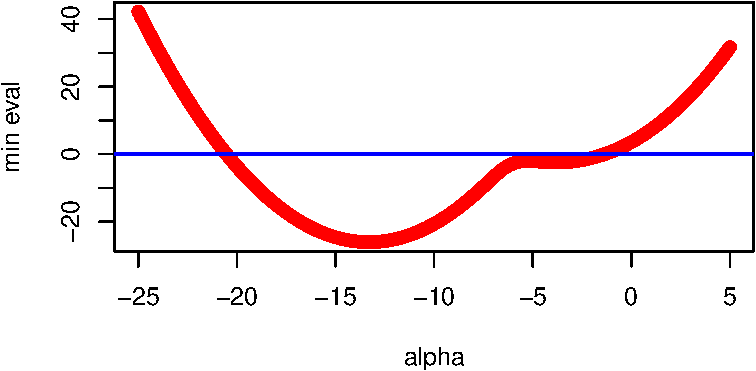
\includegraphics{interval_files/figure-pdf/gruadd-1.pdf}

\begin{verbatim}
 [1] -20.527411+0.0000000i -10.174103+0.0000000i  -9.472504+0.0000000i
 [4]  -6.622263+0.3526193i  -6.622263-0.3526193i  -5.885691+0.2875441i
 [7]  -5.885691-0.2875441i  -5.640580+0.3668888i  -5.640580-0.3668888i
[10]  -4.391289+0.2532477i  -4.391289-0.2532477i  -3.708911+0.3868444i
[13]  -3.708911-0.3868444i  -3.238930+0.0000000i  -2.311379+0.0000000i
[16]  -1.369315+0.0000000i
\end{verbatim}

\subsubsection{Ekman Example}\label{ekman-example}

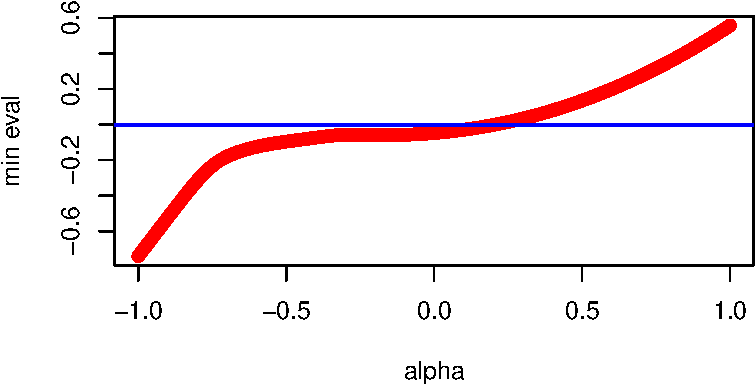
\includegraphics{interval_files/figure-pdf/ekkadd-1.pdf}

\begin{verbatim}
 [1] -5.713009655+0.00000000i -3.782729083+0.00000000i -1.791313475+0.00000000i
 [4] -1.628964140+0.00000000i -0.976213035+0.00000000i -0.744289350+0.04959388i
 [7] -0.744289350-0.04959388i -0.682321433+0.00000000i -0.534849034+0.00000000i
[10] -0.513033529+0.00000000i -0.497908376+0.02481447i -0.497908376-0.02481447i
[13] -0.372321687+0.13138923i -0.372321687-0.13138923i -0.388308013+0.00000000i
[16] -0.229813135+0.18259852i -0.229813135-0.18259852i -0.286712033+0.00000000i
[19] -0.212601059+0.11851989i -0.212601059-0.11851989i  0.206312577+0.00000000i
[22] -0.194299448+0.00000000i  0.132767430+0.00000000i -0.079646956+0.00000000i
[25] -0.024193535+0.00000000i -0.006762279+0.00000000i
\end{verbatim}

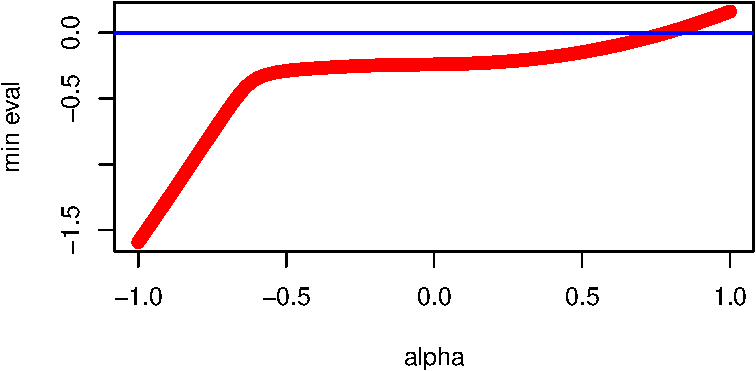
\includegraphics{interval_files/figure-pdf/ekk3add-1.pdf}

\begin{verbatim}
 [1] -7.974065161+0.00000000i -4.867929358+0.00000000i -1.224234244+0.00000000i
 [4] -0.982237601+0.00000000i  0.785644808+0.00000000i  0.648677529+0.00000000i
 [7] -0.554033177+0.00000000i -0.542600618+0.01297027i -0.542600618-0.01297027i
[10]  0.486418243+0.00000000i -0.111892110+0.39235860i -0.111892110-0.39235860i
[13]  0.382974612+0.00000000i  0.353089664+0.00000000i -0.351610318+0.00000000i
[16] -0.307360690+0.00000000i -0.126594060+0.26307892i -0.126594060-0.26307892i
[19] -0.073544792+0.26986305i -0.073544792-0.26986305i -0.233302697+0.00000000i
[22] -0.008137562+0.19480062i -0.008137562-0.19480062i -0.138025415+0.11750706i
[25] -0.138025415-0.11750706i  0.120502647+0.00000000i
\end{verbatim}

\subsection{A Variation}\label{variation}

Alternatively, we could define our approximation problem as finding
\(X\in\mathbb{R}^{n\times p}\) and \(\alpha\) such that
\(\sqrt{\delta_{ij}^2+\alpha}\approx d_{ij}(X)\), or, equivalently,
\(\Delta\times\Delta+\alpha(E-I)\approx D(X)\times D(X)\).

\begin{Shaded}
\begin{Highlighting}[]
\NormalTok{For any $X\textbackslash{}in\textbackslash{}mathbb\{R\}\^{}\{n\textbackslash{}times p\}$ with $p=n{-}2$ there is an $\textbackslash{}alpha$}
\NormalTok{such that $\textbackslash{}sqrt\{\textbackslash{}delta\_\{ij\}\^{}2+\textbackslash{}alpha\}= d\_\{ij\}(X)$.}
\end{Highlighting}
\end{Shaded}

\begin{proof}
Now we have

\begin{equation}
\tau(\Delta\times\Delta+\alpha(E-I)))=
  \tau(\Delta\times\Delta)+\frac12\alpha J.
(\#eq:tau2)
\end{equation}

The eigenvalues of \(\tau(\Delta\times\Delta)+\frac12\alpha J\) are zero
and \(\lambda_s+\frac12\alpha\), where the \(\lambda_s\) are the \(n-1\)
non-trivial eigenvalues of \(\tau(\Delta\times\Delta)\). If
\(\underline{\lambda}\) is smallest eigenvalue we choose
\(\alpha=-2\underline{\lambda}\), and
\(\tau(\Delta\times\Delta)+\frac12\alpha J\) is positive semi-definite
of rank \(r\leq n-2\).
\end{proof}

Note that theorem @ref(thm:nmn2) implies that for any \(\Delta\) there
is a strictly increasing differentiable transformation to the space of
Euclidean distance matrices in \(n-2\) dimensions. This is a version of
what is sometimes described as \emph{Guttman's n-2 theorem} (Lingoes
(\citeproc{ref-lingoes_71}{1971})). The proof we have given is that from
De Leeuw (\citeproc{ref-deleeuw_R_70b}{1970}), Appendix B.

\section{Interval smacof}\label{interval-smacof}

In this section we introduce a double-phase alternating least squares
algorithm that fits better into the smacof framework than the
single-phase method proposed by Cooper (\citeproc{ref-cooper_72}{1972}).
We also restrict our linear transformations to be to be increasing and
non-negative on the positive real axes.

To avoid various kinds of trivialities, assume not all \(d_{ij}(X)\) are
zero.

In the optimal scaling phase we must minimize

\begin{equation}
\sigma(X,\alpha,\beta)=\mathop{\sum\sum}_{1\leq i<j\leq  n}w_{ij}(\alpha\delta_{ij}+\beta-d_{ij}(X))^2
(\#eq:intloss)
\end{equation}

The constraints are \(\alpha\delta_{ij}+\beta\geq 0\) and
\(\alpha\delta_{ij}+\beta\geq\alpha\delta_{kl}+\beta\) if
\(\delta_{ij}\geq\delta_{kl}\). These define pointed convex cone in the
space of disparities. We need to project \(D(X)\) on that cone, in the
metric defined by \(W\). But it is easy to see that and equivalent set
of constraints in \(\mathbb{R}^2\) is \(\alpha\geq 0\) and
\(\alpha\delta_\text{min}+\beta\geq 0\). Again these two constraints
define a pointed cone in two-dimensional \((\alpha,\beta)\) space, where
proje ction is much easier to handle thanin the generally much larger
disparity space. Of course the projection metric in \((\alpha,\beta)\)
is different from the one in disparity space.

In addition to the inequality constraints we have the normalization
constraint \begin{equation}
\mathop{\sum\sum}_{1\leq i<j\leq  n}w_{ij}(\alpha\delta_{ij}+\beta)^2=1,
(\#eq:intnorm)
\end{equation} but as we have seen in chapter @ref(nonmtrmds) we can
initially ignore that constraint, project on the cone, and then
normalize the projection.

In order to simplify the notation we collect the \(d_{ij}(X)\) in a
vector \(d\), the \(\delta_{ij}\) in a vector \(\delta\) and the
\(w_{ij}\) in a diagonal matrix \(W\).

Let's first get the trivial case where all \(\delta_{ij}\) are equal out
of the way. In that case the linear regression is singular, and we
simply choose all \(\alpha\delta+\beta\) equal to the constant \(e'Wd\),
for example by setting \(\alpha=0\) and \(\beta=e'Wd\). Applying the
normalization condition @ref(eq:intnorm) then sets \(\beta=1\). From now
on we assume in this section that not all \(\delta_{ij}\) are equal.

Projecting on the cone gives us four possibilities. We can have
\(\alpha=0\) or \(\alpha\delta_\text{min}+\beta=0\), or both, or
neither. We first analyze the case in which the unconstrained minimum of
@ref(eq:intloss) is in the cone, which will be the most common case,
especially in later smacof iterations. Using the fact that
\(\delta'W\delta=e'We=1\) we find that \begin{equation}
\begin{bmatrix}\tilde\alpha\\\tilde\beta\end{bmatrix}=
\frac{1}{1-(e'W\delta)^2}\begin{bmatrix}\delta'(W-We e'W)d\\e'(W-W\delta\delta'W)d\end{bmatrix}.
(\#eq:intunc)
\end{equation} If \(\tilde\alpha\geq 0\) and
\(\tilde\beta\geq-\alpha\delta_\text{min}\) we are done. If not, we know
the projection is on the line \(\alpha=0\) or on the line
\(\tilde\beta=-\alpha\delta_\text{min}\), or on their intersection,
which is the origin.

First suppose the projection is on \(\alpha=0\). We find the minimizing
\(\beta\) equal to \(\overline{\beta}:=e'Wd\), which strictly satisfies
the second constraint because
\(\overline\beta>-\alpha\delta_\text{min}=0\), and thus \((0,e'Wd)\) is
on the boundary of the cone. This also show that the origin, which has
\(\sigma(X,0,0)=d'Wd\), can never be the projection. The minimum at
\((0,e'Wd)\) is \begin{equation}
\sigma(X,0,e'Wd)=d'Wd-(d'We)^2
(\#eq:intvertexloss1)
\end{equation} Or, alternatively, we can assume that the projection is
on the vertex \(\beta=-\alpha\delta_\text{min}\), in which case the
minimizing \(\alpha\) is \begin{equation}
\overline{\alpha}:=\frac{(\delta-\delta_\text{min})'Wd}{(\delta-\delta_\text{min})'W(\delta-\delta_\text{min})},
(\#eq:intalpha)
\end{equation} which is always positive, and thus
\((\overline{\alpha},-\overline{\alpha}\delta_\text{min})\) is on the
boundary of the cone. The minimum is \begin{equation}
\sigma(X,\overline{\alpha},-\overline{\alpha}\delta_\text{min})=d'Wd-\frac{((\delta-\delta_\text{min})'Wd)^2}{(\delta-\delta_\text{min})'W(\delta-\delta_\text{min})}
(\#eq:intvertexloss2)
\end{equation} If the unconstrained solution is not in the cone, then we
choose the projection as the solution corresponding with the smallest of
@ref(eq:intvertexloss1) and (@ref(eq:intvertexloss2).

\subsection{Example}\label{example}

We illustrate finding the optimal linear transformation with a small
example. We choose some arbitrary \(w\), \(\delta\), and \(d\) and
normalize them in the usual way.

\begin{Shaded}
\begin{Highlighting}[]
\NormalTok{w }\OtherTok{\textless{}{-}} \FunctionTok{c}\NormalTok{(}\FunctionTok{rep}\NormalTok{(}\DecValTok{1}\NormalTok{,}\DecValTok{5}\NormalTok{),}\FunctionTok{rep}\NormalTok{(}\DecValTok{2}\NormalTok{,}\DecValTok{5}\NormalTok{))}
\NormalTok{w }\OtherTok{\textless{}{-}}\NormalTok{ w }\SpecialCharTok{/} \FunctionTok{sum}\NormalTok{(w)}
\NormalTok{delta }\OtherTok{\textless{}{-}} \DecValTok{1}\SpecialCharTok{:}\DecValTok{10}
\NormalTok{s }\OtherTok{\textless{}{-}} \FunctionTok{sum}\NormalTok{(w }\SpecialCharTok{*}\NormalTok{ delta }\SpecialCharTok{\^{}} \DecValTok{2}\NormalTok{)}
\NormalTok{delta }\OtherTok{\textless{}{-}}\NormalTok{ delta }\SpecialCharTok{/} \FunctionTok{sqrt}\NormalTok{ (s)}
\NormalTok{d }\OtherTok{\textless{}{-}} \FunctionTok{c}\NormalTok{(}\DecValTok{1}\NormalTok{, }\DecValTok{2}\NormalTok{, }\DecValTok{3}\NormalTok{, }\DecValTok{4}\NormalTok{, }\DecValTok{4}\NormalTok{, }\DecValTok{3}\NormalTok{, }\DecValTok{3}\NormalTok{, }\DecValTok{3}\NormalTok{, }\DecValTok{1}\NormalTok{, }\DecValTok{1}\NormalTok{)}
\NormalTok{s }\OtherTok{\textless{}{-}} \FunctionTok{sum}\NormalTok{ (w }\SpecialCharTok{*}\NormalTok{ d }\SpecialCharTok{\^{}} \DecValTok{2}\NormalTok{)}
\NormalTok{t }\OtherTok{\textless{}{-}} \FunctionTok{sum}\NormalTok{ (w }\SpecialCharTok{*}\NormalTok{ d }\SpecialCharTok{*}\NormalTok{ delta)}
\NormalTok{d }\OtherTok{\textless{}{-}}\NormalTok{ d }\SpecialCharTok{*}\NormalTok{ (t }\SpecialCharTok{/}\NormalTok{ s)}
\end{Highlighting}
\end{Shaded}

After normalization the \(\delta_{\text{min}}\) is 0.1448414. The pink
region in figure @ref(fig:intconex) is the cone formed by the
intersection of the half-spaces \(\alpha\geq 0\) and
\(\alpha\delta_{\text{min}}+\beta\geq 0\).

\begin{figure}[H]

{\centering 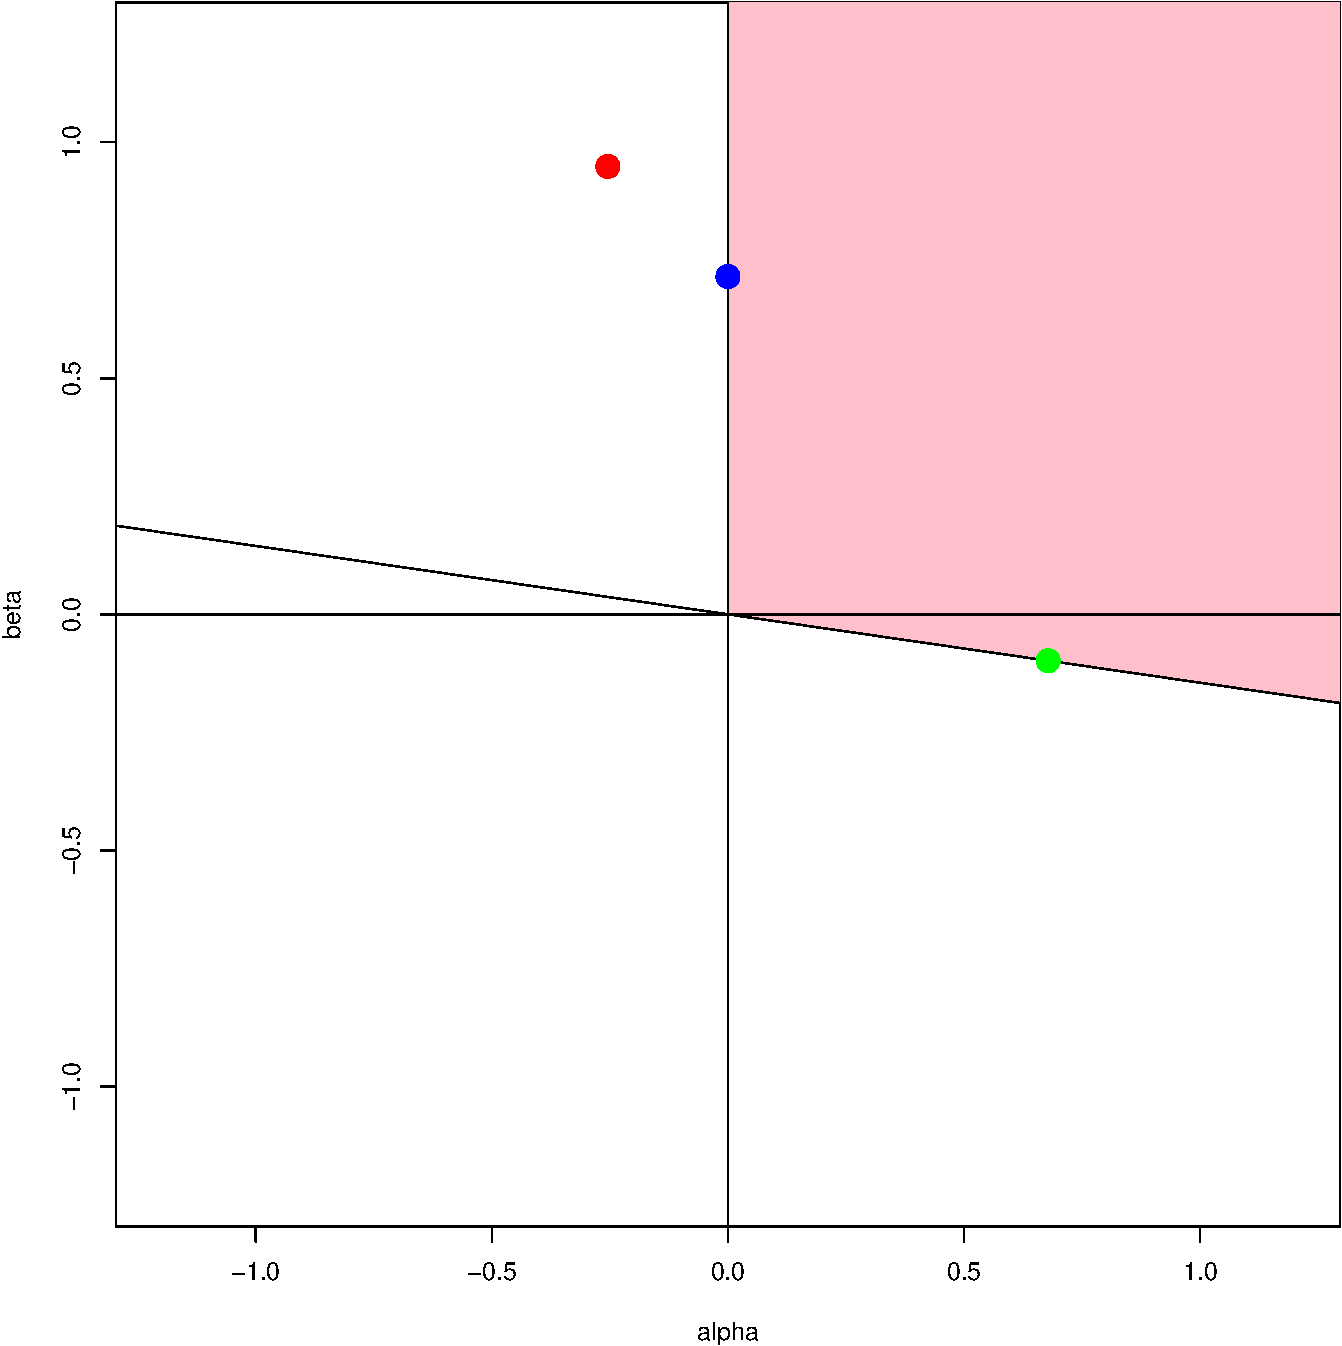
\includegraphics{interval_files/figure-pdf/intconex-1.pdf}

}

\caption{Cone Projection}

\end{figure}%

The unconstrained minimum is attained at -0.2541855, 0.9484652, the red
point in figure @ref(fig:intconex), with stress equal to 0.0939827. That
is clearly outside the cone, so we now consider projection on the two
one-dimensional boundary rays. The blue point is 0, 0.7152935, the
projection on \(\alpha\geq 0\). It is fairly close to the unconstrained
minimum, with stress 0.1042239. The green point 0.6782764, -0.0982425is
the projection on \(\beta=-\alpha\delta_{\text{min}}\), which has stress
0.2684117. Thus the blue point 0, 0.7152935is the actual projection on
the cone in \((\alpha,\beta)\) space, and the best fitting line has
slope zero (which, in smacof, would make all disparities equal for the
next iteration).

This is illustrated in a different way (with Shepard plots) in figure
@ref(fig:intlineex), where we see the red, blue, and green lines
corresponding with the red, blue, and green points in figure
@ref(fig:intconex). Note that the green line goes through the point
\((\delta_{\text{min}},0)\). The horizontal blue line is the best
fitting one under the constraints.

\begin{figure}[H]

{\centering 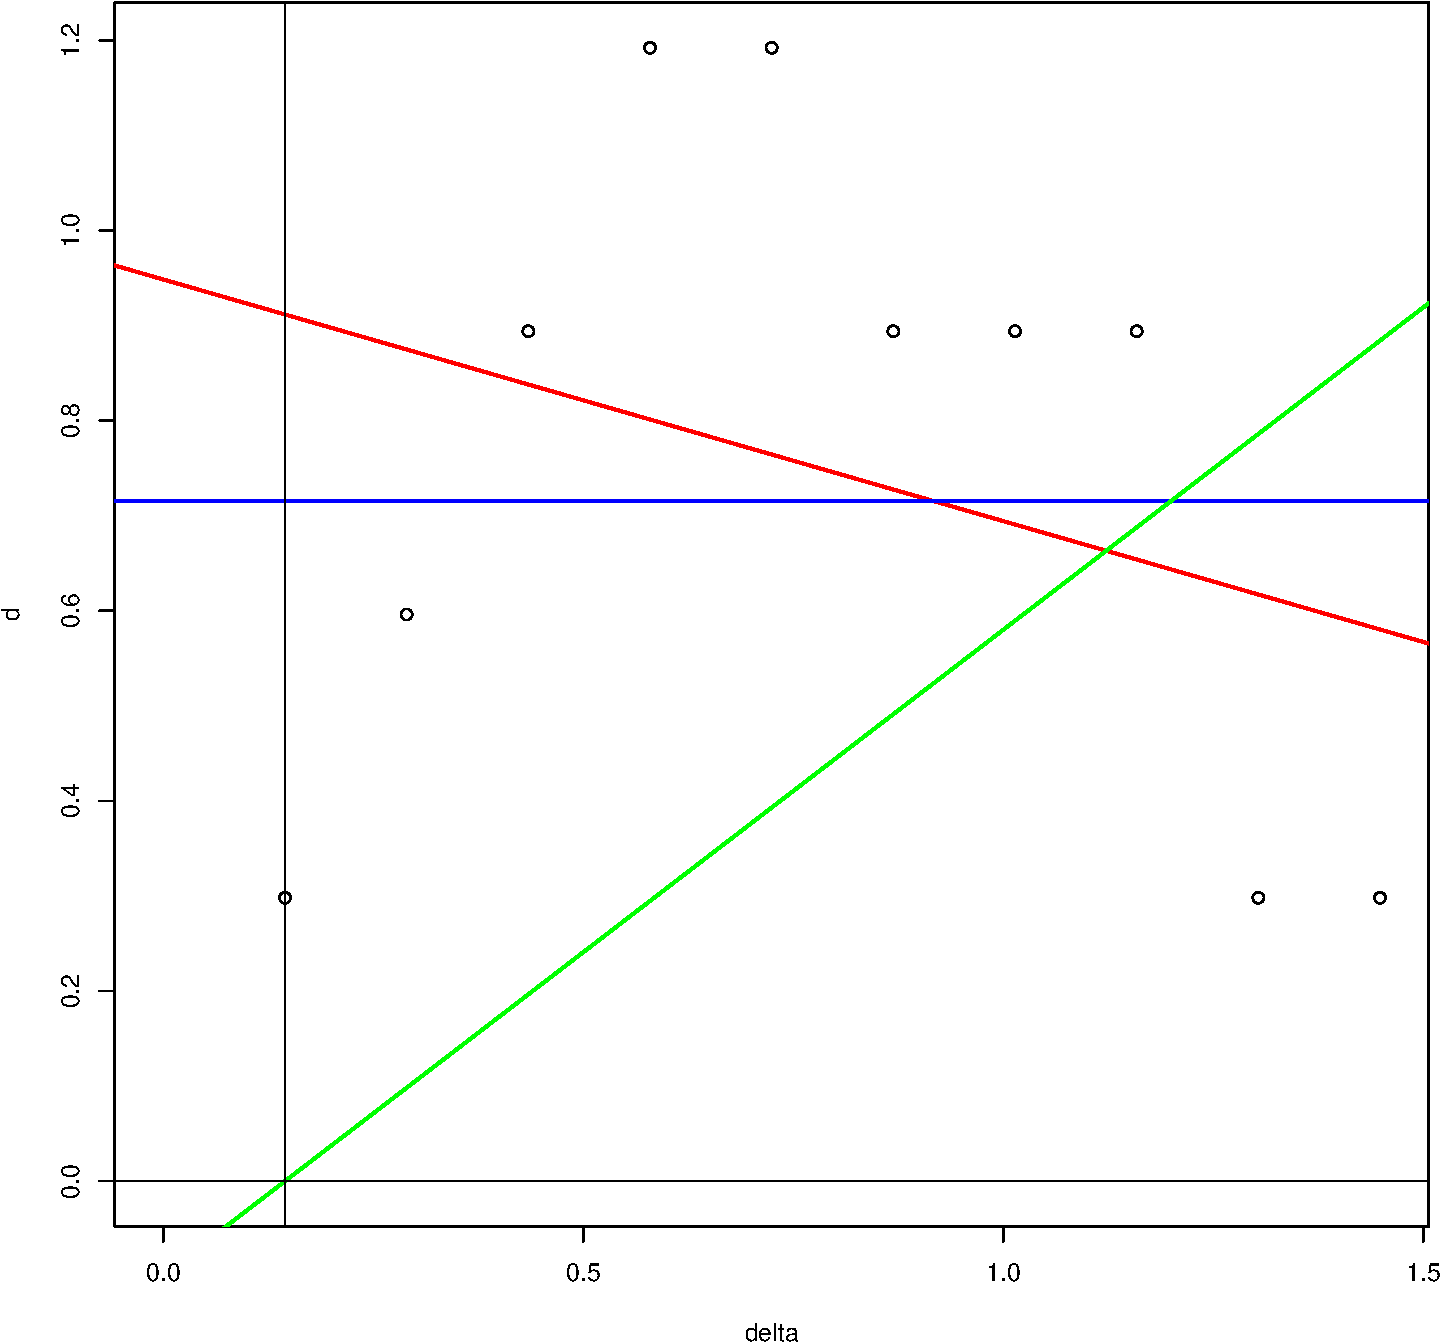
\includegraphics{interval_files/figure-pdf/intlineex-1.pdf}

}

\caption{Fitted Lines}

\end{figure}%

\bookmarksetup{startatroot}

\chapter{Polynomial MDS}\label{polynomial-mds}

\section{Introduction}\label{introduction}

\section{Fitting Polynomials}\label{fitting-polynomials}

\[
\sigma(X)=\mathop{\sum\sum}_{1\leq i<j\leq n}w_{ij}(P_r(\delta_{ij})-d_{ij}(X))^2
\]

\[
P_r(\delta_{ij}):=\sum_{s=0}^r\alpha_s^{\ }\delta_{ij}^s.
\]

The polynomial \(P_r\) is \emph{tied down} if \(\alpha_0=0\), and thus
\(P_r(0)=0\).

Vandermonde matrix

\section{Positive and Convex, Monotone
Polynomials}\label{positive-and-convex-monotone-polynomials}

\subsection{Introduction}\label{introduction-1}

Constraints on values, constraints on coefficients

\begin{Shaded}
\begin{Highlighting}[]
\NormalTok{f }\OtherTok{\textless{}{-}} \ControlFlowTok{function}\NormalTok{(x) }\FunctionTok{return}\NormalTok{(x }\SpecialCharTok{*}\NormalTok{ (x }\SpecialCharTok{{-}} \DecValTok{1}\NormalTok{) }\SpecialCharTok{*}\NormalTok{ (x }\SpecialCharTok{{-}} \DecValTok{2}\NormalTok{))}
\NormalTok{x }\OtherTok{\textless{}{-}} \FunctionTok{seq}\NormalTok{(}\DecValTok{0}\NormalTok{, }\DecValTok{3}\NormalTok{, }\AttributeTok{length =} \DecValTok{100}\NormalTok{)}
\NormalTok{y }\OtherTok{\textless{}{-}} \FunctionTok{f}\NormalTok{(x)}
\FunctionTok{plot}\NormalTok{(x, y, }\AttributeTok{type=}\StringTok{"l"}\NormalTok{, }\AttributeTok{lwd =} \DecValTok{3}\NormalTok{, }\AttributeTok{col =} \StringTok{"RED"}\NormalTok{)}
\NormalTok{x }\OtherTok{\textless{}{-}} \FunctionTok{c}\NormalTok{(.}\DecValTok{10}\NormalTok{, .}\DecValTok{45}\NormalTok{, }\FloatTok{2.25}\NormalTok{, }\FloatTok{2.75}\NormalTok{)}
\NormalTok{y }\OtherTok{\textless{}{-}} \FunctionTok{f}\NormalTok{(x)}
\FunctionTok{abline}\NormalTok{(}\AttributeTok{h =}\NormalTok{ y[}\DecValTok{1}\NormalTok{])}
\FunctionTok{abline}\NormalTok{(}\AttributeTok{h =}\NormalTok{ y[}\DecValTok{2}\NormalTok{])}
\FunctionTok{abline}\NormalTok{(}\AttributeTok{h =}\NormalTok{ y[}\DecValTok{3}\NormalTok{])}
\FunctionTok{abline}\NormalTok{(}\AttributeTok{h =}\NormalTok{ y[}\DecValTok{4}\NormalTok{])}
\FunctionTok{abline}\NormalTok{(}\AttributeTok{v =}\NormalTok{ x[}\DecValTok{1}\NormalTok{])}
\FunctionTok{abline}\NormalTok{(}\AttributeTok{v =}\NormalTok{ x[}\DecValTok{2}\NormalTok{])}
\FunctionTok{abline}\NormalTok{(}\AttributeTok{v =}\NormalTok{ x[}\DecValTok{3}\NormalTok{])}
\FunctionTok{abline}\NormalTok{(}\AttributeTok{v =}\NormalTok{ x[}\DecValTok{4}\NormalTok{])}
\end{Highlighting}
\end{Shaded}

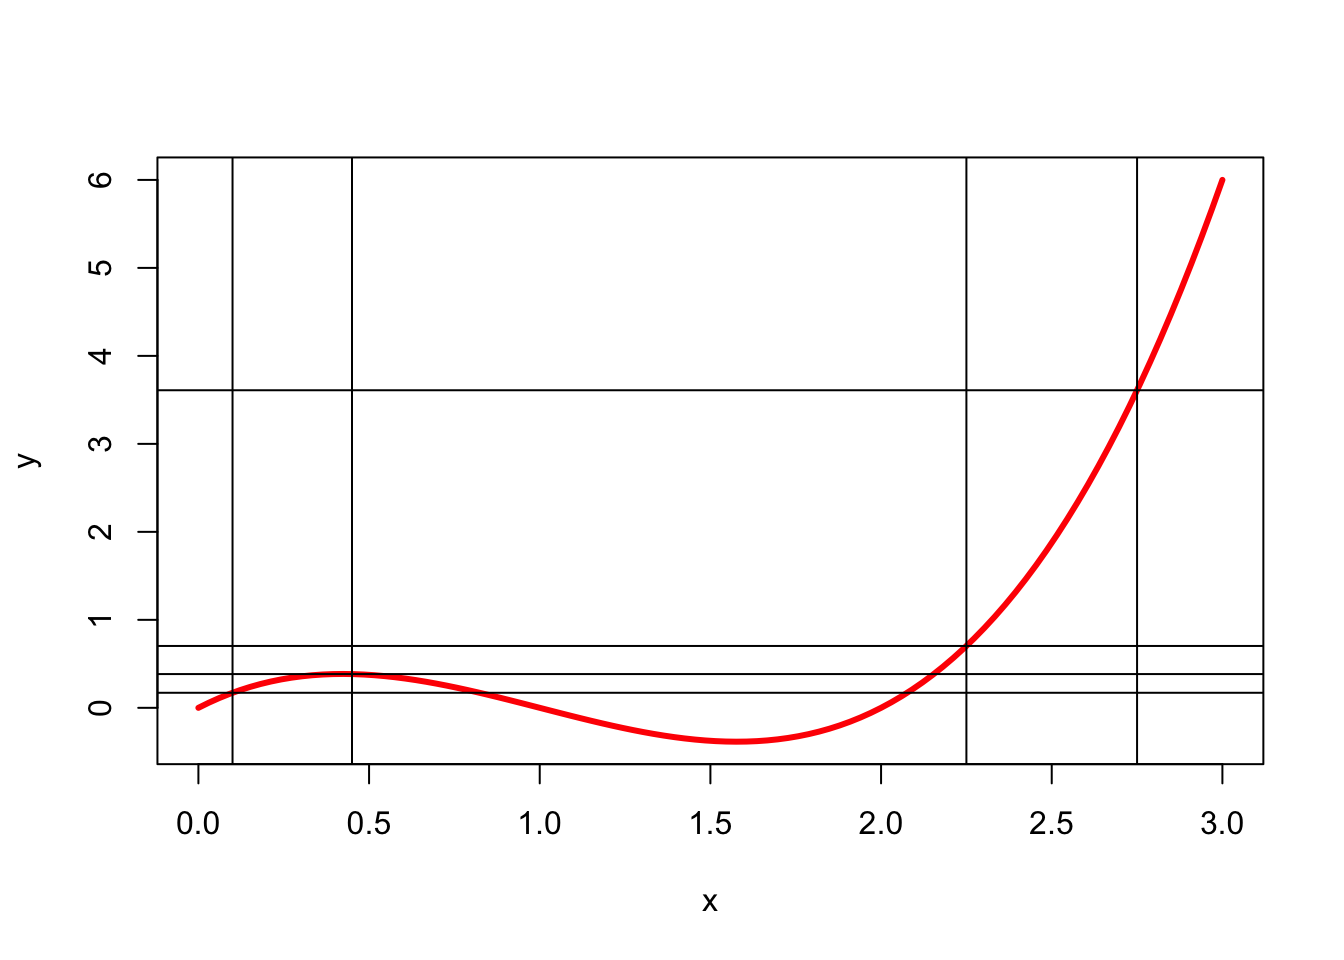
\includegraphics{polynomial_files/figure-pdf/unnamed-chunk-2-1.pdf}

Tied-down increasing non-negative cubic.

Write the tied-down cubic in the form \(f(x)=ax(x^2+2bx+c)\). Since we
must have \(f(x)\rightarrow+\infty\) of \(x\rightarrow+\infty\) we have
\(a>0\). Since \(f\) must be increasing at zero, we must have
\(f'(0)=c>0\). No real roots on the positive reals. Case 1: no real
roots at all \(b^2-c<0\). Case 2: two real roots, both negative
\(b^2-c\geq 0\) and \(b\geq 0\). Since \(c>0\) the product of roots is
positive. If the sum is negative, i.e.~if \(b>0\) both roots are
negative. Since \(f''(x)=6x+b\) we see that \(f\) is convex on the
positive real axis if \(b\geq 0\).

\subsection{A QP Algorithm}\label{a-qp-algorithm}

In this section we construct an algorithm for a general weighted linear
least squares projection problem with equality and/or inequality
constraints. It uses duality and unweighting majorization. The section
takes the form of a small diversion, with examples. This may seem
somewhat excessive, but it provides an easy reference for both you and
me and it serves as a manual for the corresponding R code.

We start with the \emph{primal problem}, say problem \(\mathcal{P}\),
which is minimizing

\begin{equation}
f(x)=\frac12(Hx-z)'V(Hx-z)
(\#eq:qpbase)
\end{equation}

over all \(x\) satisfying equalities \(Ax\geq b\) and equations
\(Cx=d\). We suppose the \emph{Slater condition} is satisfied,
i.e.~there is an \(x\) such that \(Ax>b\). And, in addition, we suppose
the system of inequalities and equations is \emph{consistent}, i.e.~has
at least one solution.

We first reduce the primal problem to a simpler, and usually smaller,
one by partitioning the loss function. Define

\begin{align}
\begin{split}
W&:=H'VH,\\
y&:=W^{-1}H'Vz,\\
Q&:=(I-H(H'VH)^{-1}H'V).\\
\end{split}
(\#eq:qpfirstpart)
\end{align}

Then

\begin{equation}
(Hx-y)'V(Hx-y)=(x-y)'W(x-y)+y'Q'VQy,
(\#eq:qpsimple)
\end{equation}

The simplified primal problem \(\mathcal{P}'\) is to minimize
\((x-y)'W(x-y)\) over \(Ax\geq b\) and \(Cx=d\), where \(W\) is assumed
to be positive definite. Obviously the solutions to \(\mathcal{P}\) and
\(\mathcal{P}'\) are the same. The two loss function values only differ
by the constant term \(y'Q'VQy\).

We do not solve \(\mathcal{P}'\) drectly, but we use Lagrangian duality
and solve the dual quadratic programmng problem. The Lagrangian for
\(\mathcal{P}'\) is

\begin{equation}
\mathcal{L}(x,\lambda,\mu)=\frac12(x-y)'W(x-y)-
\lambda'(Ax - b)-\mu'(Cx-d),
(\#eq:qplagrange)
\end{equation}

where \(\lambda\geq 0\) and \(\mu\) are the Lagrange multipliers.

Now

\begin{align}
\begin{split}
\max_{\lambda\geq 0}\max_\mu\mathcal{L}(x,\lambda,\mu)&=\\
&=\begin{cases}\frac12(x-y)'W(x-y)-\lambda'(Ax - b)-\mu'(Cx-d)&\text{ if }Ax\geq b,\\
+\infty&\text{ otherwise},
\end{cases}
\end{split}
(\#eq:qpxcalc1)
\end{align}

and thus

\begin{equation}
\min_x\max_{\lambda\geq 0}\max_\mu\mathcal{L}(x,\lambda,\mu)=\min_{Ax\geq b}\min_{Cx=d}\frac12(x-y)'W(x-y),
(\#eq:qpxcalc2)
\end{equation}

which is our original simplified primal problem \(\mathcal{P}'\).

We now look at the \emph{dual problem} \(\mathcal{D}'\) (of
\(\mathcal{P}'\)), which means solving

\begin{equation}
\max_{\lambda\geq 0}\max_\mu\min_x\mathcal{L}(x,\lambda,\mu).
(\#eq:qpdual)
\end{equation}

The inner minimum over \(x\) for given \(\lambda\) and \(\mu\) is
attained at

\begin{equation}
x=y+W^{-1}(A'\mid C')\begin{bmatrix}\lambda\\\mu\end{bmatrix},
(\#eq:qpxsolve)
\end{equation}

and is equal to \(-g(\lambda,\mu)\), where

\begin{equation}
\frac12\begin{bmatrix}\lambda&\mu\end{bmatrix}
\begin{bmatrix}AW^{-1}A'&AW^{-1}C'\\CW^{-1}A'&CW^{-1}C'\end{bmatrix}\begin{bmatrix}\lambda\\\mu\end{bmatrix}+\\
+\lambda'(Ay-b)\\
+\mu'(Cy-d)
(\#eq:qpdualf)
\end{equation}

Our strategy is to solve \(\mathcal{D'}\) for \(\lambda\geq 0\) and/or
\(\mu\). Because of our biases we do not maximize \(-g\), we minimize
\(g\). Then compute the solution of both \(\mathcal{P}'\) and
\(\mathcal{P}\) from @ref(eq:qpxsolve). The duality theorem for
quadratic programming tells us the values of \(f\) at the optimum of
\(\mathcal{P}'\) and \(-g\) at the optimum of \(\mathcal{D}'\) are
equal, and of course the value at the optimum of \(\mathcal{P}\) is that
of \(\mathcal{P}'\) plus the constant \(y'QVQy\).

From here on we can proceed with unweighting in various ways. We could,
for instance, minimize out \(\mu\) and then unweight the resulting
quadratic form. Instead, we go the easy way. Majorize the partitioned
matrix \(K\) in the quadratic part of @ref(eq:qpdualf) by a similarly
partitioned diagonal positive matrix \(E\).

\begin{equation}
E:=\begin{bmatrix}F&\emptyset\\\emptyset&G\end{bmatrix}\gtrsim K:=\begin{bmatrix}AW^{-1}A'&AW^{-1}C'\\CW^{-1}A'&CW^{-1}C'\end{bmatrix}
(\#eq:qpdumaj)
\end{equation}

Suppose \(\tilde\lambda\geq 0\) and \(\tilde\mu\) are the current best
solutions of the dual problem. Put them on top of each other to define
\(\tilde\gamma\), and do the same with \(\lambda\) and \(\mu\) to get
\(\gamma\). Then \(g(\lambda,\mu)\) becomes

\begin{equation}
\frac12 (\tilde\gamma+(\gamma-\tilde\gamma))'E(\tilde\gamma+(\gamma-\tilde\gamma))+\gamma'(Ry-e)=\\
=\frac12(\gamma-\tilde\gamma)'E(\gamma-\tilde\gamma)+ (\gamma-\tilde\gamma)'E(\tilde\gamma+(Ry-e))+\\+\frac12\tilde\gamma'E\tilde\gamma+\tilde\gamma'(Ry-e)
(\#eq:qpdualcomp)
\end{equation}

The last two terms do not depend on \(\gamma\), so for the majorization
algorithm is suffices to minimize

\begin{equation}
\frac12(\gamma-\tilde\gamma)'F(\gamma-\tilde\gamma)+ (\gamma-\tilde\gamma)'E(\tilde\gamma+(Ry-e))
(\#eq:qpdualproj)
\end{equation}

Let

\begin{equation}
\xi:=\tilde\gamma-F^{-1}E(\tilde\gamma+(Ry-e))
(\#eq:qpdefxi)
\end{equation}

then @ref(eq:qpdualproj) becomes

\begin{equation}
\frac12(\gamma-\xi)'F(\gamma-\xi)-\frac12\xi'F\xi
(\#eq:qpdualsimp)
\end{equation}

Because \(F\) is diagonal \(\lambda_i=\max(0,\xi_i)\) for
\(i=1,\cdots m_1\) and and \(\mu_i=\xi_{i+m_1}\) for \(i=1,\cdots m_2\).

Section @ref(apcodemathadd) has the R code for qpmaj(). The defaults are
set to do a simple isotone regression, but of course the function has a
much larger scope. It can handle equality constraints, linear convexity
constraints, partial orders, and much more general linear inequalities.
It can fit polynomials, monotone polynomials, splnes, and monotone
splines of various sorts. It is possible to have only inequality
constraints, only equality constraints, or both. The matrix \(H\) of
predictors in @ref(eq:qpbase) can either be there or not be there.

The function qpmaj() returns both \(x\) and \(\lambda\), and the values
of \(\mathcal{P}\), \(\mathcal{P}'\), and \(\mathcal{D}'\). And also the
\emph{predicted values} \(Hx\), and the \emph{constraint values}
\(Ax-b\) and \(Cx-d\), if applicable. It's always nice to check
\emph{complimentary slackness} \(\lambda'(Ax-b)=0\), and another check
is provided because the values of \(\mathcal{P}'\) and \(\mathcal{D}'\)
must be equal. Finally qpmaj() returns the number of iterations for the
dual problem.

The function qpmaqj() does not have the pretense to compete in
efficiency with the sophisticated pivoting and active set strategies for
quadratic programming discussed for example by Best
(\citeproc{ref-best_17}{2017}). But it seems to do a reliable job on our
small examples, and it is an interesting example of majorization and
unweighting.

\subsubsection{Example 1: Simple Monotone
Regression}\label{example-1-simple-monotone-regression}

Here are the two simple monotone regression examples from section
@ref(mathsimpiso), the first one without weights and the second one with
a diagonal matrix of weights.

\begin{Shaded}
\begin{Highlighting}[]
\NormalTok{y}\OtherTok{\textless{}{-}}\FunctionTok{c}\NormalTok{(}\DecValTok{1}\NormalTok{,}\DecValTok{2}\NormalTok{,}\DecValTok{1}\NormalTok{,}\DecValTok{3}\NormalTok{,}\DecValTok{2}\NormalTok{,}\SpecialCharTok{{-}}\DecValTok{1}\NormalTok{,}\DecValTok{3}\NormalTok{)}
\FunctionTok{qpmaj}\NormalTok{(y)}
\end{Highlighting}
\end{Shaded}

\begin{verbatim}
$x
[1] 1.0 1.4 1.4 1.4 1.4 1.4 3.0

$fprimal
[1] 4.6

$fdual
[1] 4.6

$lambda
[1] 0.0000000 0.5999999 0.1999999 1.7999999 2.3999999 0.0000000

$inequalities
[1]  4.000001e-01 -2.760349e-08 -4.466339e-08 -4.466339e-08 -2.760349e-08
[6]  1.600000e+00

$itel
[1] 146
\end{verbatim}

\begin{Shaded}
\begin{Highlighting}[]
\FunctionTok{qpmaj}\NormalTok{(y, }\AttributeTok{v =} \FunctionTok{diag}\NormalTok{(}\FunctionTok{c}\NormalTok{(}\DecValTok{1}\NormalTok{,}\DecValTok{2}\NormalTok{,}\DecValTok{3}\NormalTok{,}\DecValTok{4}\NormalTok{,}\DecValTok{3}\NormalTok{,}\DecValTok{2}\NormalTok{,}\DecValTok{1}\NormalTok{)))}
\end{Highlighting}
\end{Shaded}

\begin{verbatim}
$x
[1] 1.000000 1.400000 1.400000 1.777778 1.777778 1.777778 3.000000

$fprimal
[1] 11.37778

$fdual
[1] 11.37778

$lambda
[1] 0.000000 1.200000 0.000000 4.888889 5.555555 0.000000

$inequalities
[1]  4.000000e-01  0.000000e+00  3.777778e-01 -4.294379e-08 -2.976007e-08
[6]  1.222222e+00

$itel
[1] 81
\end{verbatim}

\subsubsection{Example 2: Monotone Regression with
Ties}\label{example-2-monotone-regression-with-ties}

Now suppose the data have tie-blocks, which we indicate with
\(\{1\}\leq\{2,3,4\}\leq\{5,6\}\leq\{7\}\). The Hasse diagram of the
partial order (courtesy of Ciomek (\citeproc{ref-ciomek_17}{2017})) is

\begin{center}
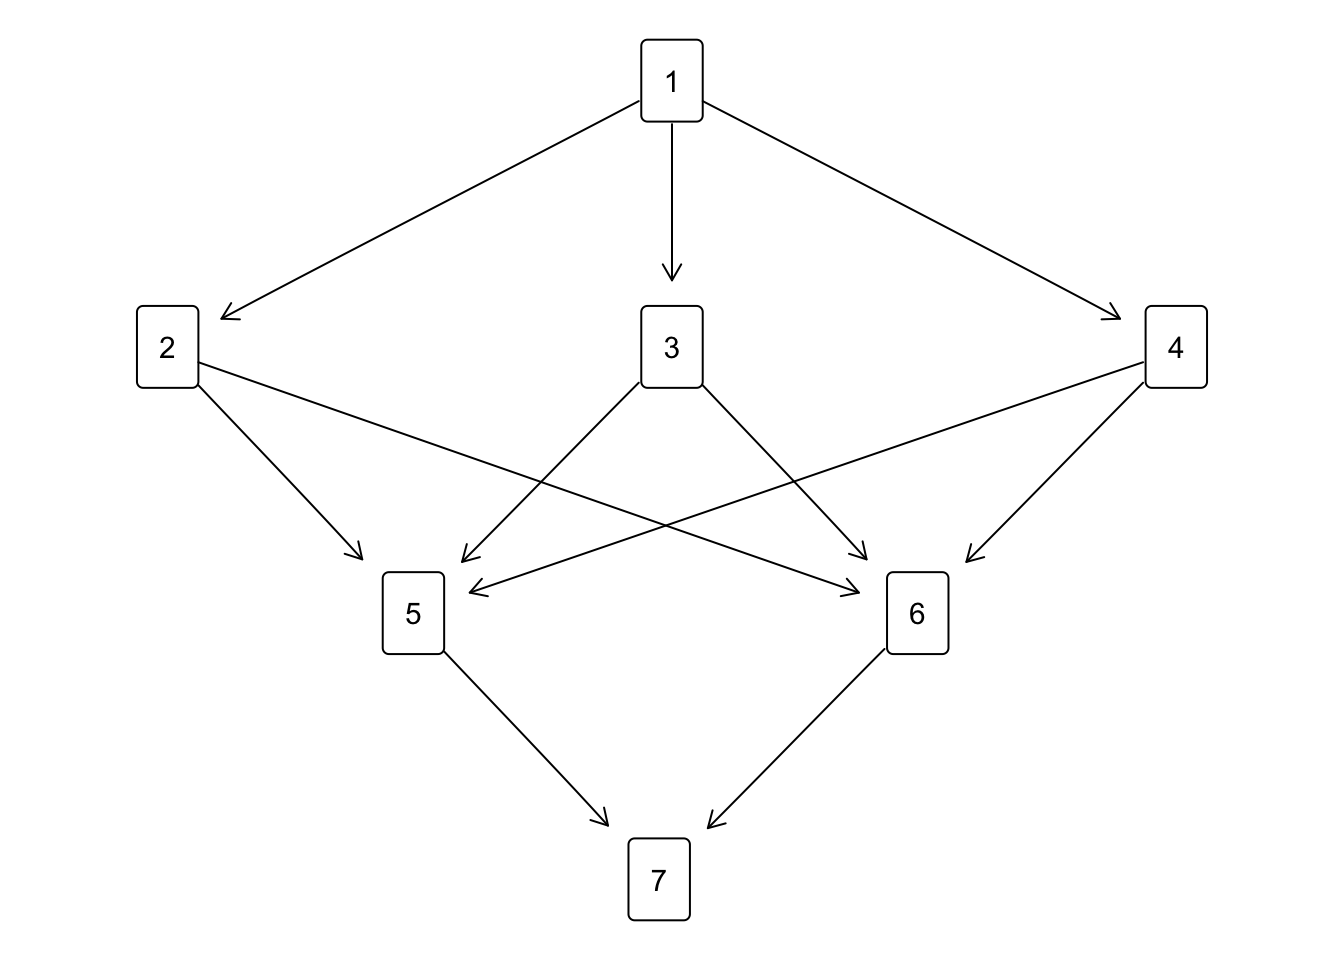
\includegraphics{polynomial_files/figure-pdf/hasse-1.pdf}
\end{center}

In the primary approach to ties the inequality constraints \(Ax\geq 0\)
are coded with \(A\) equal to

\begin{verbatim}
      [,1] [,2] [,3] [,4] [,5] [,6] [,7]
 [1,]   -1   +1   +0   +0   +0   +0   +0
 [2,]   -1   +0   +1   +0   +0   +0   +0
 [3,]   -1   +0   +0   +1   +0   +0   +0
 [4,]   +0   -1   +0   +0   +1   +0   +0
 [5,]   +0   -1   +0   +0   +0   +1   +0
 [6,]   +0   +0   -1   +0   +1   +0   +0
 [7,]   +0   +0   -1   +0   +0   +1   +0
 [8,]   +0   +0   +0   -1   +1   +0   +0
 [9,]   +0   +0   +0   -1   +0   +1   +0
[10,]   +0   +0   +0   +0   -1   +0   +1
[11,]   +0   +0   +0   +0   +0   -1   +1
\end{verbatim}

Applying our algorithm gives

\begin{Shaded}
\begin{Highlighting}[]
\FunctionTok{qpmaj}\NormalTok{(y, }\AttributeTok{a =}\NormalTok{ a)}
\end{Highlighting}
\end{Shaded}

\begin{verbatim}
$x
[1] 1.000000 1.333333 1.000000 1.333333 2.000000 1.333333 3.000000

$fprimal
[1] 4.333333

$fdual
[1] 4.333333

$lambda
 [1] 0.000000e+00 2.069906e-15 0.000000e+00 0.000000e+00 6.666667e-01
 [6] 0.000000e+00 0.000000e+00 0.000000e+00 1.666667e+00 0.000000e+00
[11] 0.000000e+00

$inequalities
 [1]  3.333333e-01  4.107825e-15  3.333334e-01  6.666667e-01  8.182895e-08
 [6]  1.000000e+00  3.333333e-01  6.666666e-01 -8.182895e-08  1.000000e+00
[11]  1.666667e+00

$itel
[1] 96
\end{verbatim}

In the secondary approach we require \(Cx=0\), with \(C\) equal to

\begin{verbatim}
     [,1] [,2] [,3] [,4] [,5] [,6] [,7]
[1,]   +0   +1   -1   +0   +0   +0   +0
[2,]   +0   +1   +0   -1   +0   +0   +0
[3,]   +0   +0   +0   +0   +1   -1   +0
\end{verbatim}

In addition we construct \(A\) to require
\(x_1\leq x_2\leq x_5\leq x_7\). This gives

\begin{Shaded}
\begin{Highlighting}[]
\FunctionTok{qpmaj}\NormalTok{(y, }\AttributeTok{a =}\NormalTok{ a, }\AttributeTok{c =}\NormalTok{ c)}
\end{Highlighting}
\end{Shaded}

\begin{verbatim}
$x
[1] 1.0 1.4 1.4 1.4 1.4 1.4 3.0

$fprimal
[1] 4.6

$fdual
[1] 4.6

$lambda
[1] 0.0 1.8 0.0

$inequalities
[1]  4.000000e-01 -5.100425e-08  1.600000e+00

$mu
[1] -0.4  1.6 -2.4

$equations
[1] -2.055633e-08 -2.055633e-08  3.443454e-08

$itel
[1] 163
\end{verbatim}

In the tertiary approach, without weights, we require
\(x_1\leq\frac{x_2+x_3+x_4}{3}\leq\frac{x_5+x_6}{2}\leq x_7\) which
means

\begin{Shaded}
\begin{Highlighting}[]
\NormalTok{a }\OtherTok{\textless{}{-}} \FunctionTok{matrix}\NormalTok{(}\FunctionTok{c}\NormalTok{(}\SpecialCharTok{{-}}\DecValTok{1}\NormalTok{,}\DecValTok{1}\SpecialCharTok{/}\DecValTok{3}\NormalTok{,}\DecValTok{1}\SpecialCharTok{/}\DecValTok{3}\NormalTok{,}\DecValTok{1}\SpecialCharTok{/}\DecValTok{3}\NormalTok{,}\DecValTok{0}\NormalTok{,}\DecValTok{0}\NormalTok{,}\DecValTok{0}\NormalTok{,}
              \DecValTok{0}\NormalTok{,}\SpecialCharTok{{-}}\DecValTok{1}\SpecialCharTok{/}\DecValTok{3}\NormalTok{,}\SpecialCharTok{{-}}\DecValTok{1}\SpecialCharTok{/}\DecValTok{3}\NormalTok{,}\SpecialCharTok{{-}}\DecValTok{1}\SpecialCharTok{/}\DecValTok{3}\NormalTok{,}\DecValTok{1}\SpecialCharTok{/}\DecValTok{2}\NormalTok{,}\DecValTok{1}\SpecialCharTok{/}\DecValTok{2}\NormalTok{,}\DecValTok{0}\NormalTok{,}
              \DecValTok{0}\NormalTok{,}\DecValTok{0}\NormalTok{,}\DecValTok{0}\NormalTok{,}\DecValTok{0}\NormalTok{,}\SpecialCharTok{{-}}\DecValTok{1}\SpecialCharTok{/}\DecValTok{2}\NormalTok{,}\SpecialCharTok{{-}}\DecValTok{1}\SpecialCharTok{/}\DecValTok{2}\NormalTok{,}\DecValTok{1}\NormalTok{),}
              \DecValTok{3}\NormalTok{,}\DecValTok{7}\NormalTok{,}\AttributeTok{byrow =} \ConstantTok{TRUE}\NormalTok{)}
\FunctionTok{matrixPrint}\NormalTok{(a, }\AttributeTok{d =} \DecValTok{2}\NormalTok{, }\AttributeTok{w =} \DecValTok{5}\NormalTok{)}
\end{Highlighting}
\end{Shaded}

\begin{verbatim}
     [,1]  [,2]  [,3]  [,4]  [,5]  [,6]  [,7] 
[1,] -1.00 +0.33 +0.33 +0.33 +0.00 +0.00 +0.00
[2,] +0.00 -0.33 -0.33 -0.33 +0.50 +0.50 +0.00
[3,] +0.00 +0.00 +0.00 +0.00 -0.50 -0.50 +1.00
\end{verbatim}

This gives

\begin{Shaded}
\begin{Highlighting}[]
\FunctionTok{qpmaj}\NormalTok{(y, }\AttributeTok{a =}\NormalTok{ a)}
\end{Highlighting}
\end{Shaded}

\begin{verbatim}
$x
[1]  1.0  1.4  0.4  2.4  2.9 -0.1  3.0

$fprimal
[1] 1.35

$fdual
[1] 1.35

$lambda
[1] 0.0 1.8 0.0

$inequalities
[1]  4.000000e-01 -1.716935e-08  1.600000e+00

$itel
[1] 30
\end{verbatim}

\subsubsection{Example 3: Weighted
Rounding}\label{example-3-weighted-rounding}

This is a silly example in which a vector \(y=\) 0.5855288, 0.709466,
-0.1093033, -0.4534972, 0.6058875, -1.817956, 0.6300986, -0.2761841,
-0.2841597, -0.919322 is ``rounded'' so that its elements are between
\(-1\) and \(+1\). The weights \(V=W\) are a banded positive definite
matrix.

\begin{Shaded}
\begin{Highlighting}[]
\NormalTok{a}\OtherTok{\textless{}{-}}\FunctionTok{rbind}\NormalTok{(}\SpecialCharTok{{-}}\FunctionTok{diag}\NormalTok{(}\DecValTok{10}\NormalTok{),}\FunctionTok{diag}\NormalTok{(}\DecValTok{10}\NormalTok{))}
\NormalTok{b}\OtherTok{\textless{}{-}}\FunctionTok{rep}\NormalTok{(}\SpecialCharTok{{-}}\DecValTok{1}\NormalTok{, }\DecValTok{20}\NormalTok{)}
\NormalTok{w}\OtherTok{\textless{}{-}}\FunctionTok{ifelse}\NormalTok{(}\FunctionTok{outer}\NormalTok{(}\DecValTok{1}\SpecialCharTok{:}\DecValTok{10}\NormalTok{,}\DecValTok{1}\SpecialCharTok{:}\DecValTok{10}\NormalTok{,}\ControlFlowTok{function}\NormalTok{(x,y) }\FunctionTok{abs}\NormalTok{(x}\SpecialCharTok{{-}}\NormalTok{y) }\SpecialCharTok{\textless{}} \DecValTok{4}\NormalTok{), }\SpecialCharTok{{-}}\DecValTok{1}\NormalTok{, }\DecValTok{0}\NormalTok{)}\SpecialCharTok{+}\DecValTok{7}\SpecialCharTok{*}\FunctionTok{diag}\NormalTok{(}\DecValTok{10}\NormalTok{)}
\FunctionTok{qpmaj}\NormalTok{(y, }\AttributeTok{v =}\NormalTok{ w, }\AttributeTok{a =}\NormalTok{ a, }\AttributeTok{b =}\NormalTok{ b)}
\end{Highlighting}
\end{Shaded}

\begin{verbatim}
$x
 [1]  0.737345533  0.917584527  0.215666042 -0.075684750  1.000000017
 [6] -1.000000039  1.000000023  0.061944776 -0.002332657 -0.754345762

$fprimal
[1] 1.110748

$fdual
[1] 1.110749

$lambda
 [1] 0.0000000 0.0000000 0.0000000 0.0000000 0.0722112 0.0000000 0.1554043
 [8] 0.0000000 0.0000000 0.0000000 0.0000000 0.0000000 0.0000000 0.0000000
[15] 0.0000000 2.8209838 0.0000000 0.0000000 0.0000000 0.0000000

$inequalities
 [1]  2.626545e-01  8.241547e-02  7.843340e-01  1.075685e+00 -1.735205e-08
 [6]  2.000000e+00 -2.303727e-08  9.380552e-01  1.002333e+00  1.754346e+00
[11]  1.737346e+00  1.917585e+00  1.215666e+00  9.243153e-01  2.000000e+00
[16] -3.922610e-08  2.000000e+00  1.061945e+00  9.976673e-01  2.456542e-01

$itel
[1] 224
\end{verbatim}

\subsubsection{Example 4: Monotone
Polynomials}\label{example-4-monotone-polynomials}

This example has a matrix \(H\) with the monomials of degree \(1,2,3\)
on the 20 points \(1,\cdots 20\). We want to fit a third-degree
polynomial which is monotone, non-negative, and anchored at zero (which
is why we do not have a monomial of degree zero, i.e.~an intercept).
Monotonicity is imposed by \((h_{i+1}-h_{i})'x\geq 0\) and
non-negativity by \(h_1'x\geq 0\). Thus there are \(19+1\) inequality
restrictions. For \(y\) we choose points on the quadratic curve
\(y=x^2\), perturbed with random error.

\begin{Shaded}
\begin{Highlighting}[]
\FunctionTok{set.seed}\NormalTok{(}\DecValTok{12345}\NormalTok{)}
\NormalTok{h }\OtherTok{\textless{}{-}} \FunctionTok{cbind}\NormalTok{(}\DecValTok{1}\SpecialCharTok{:}\DecValTok{20}\NormalTok{,(}\DecValTok{1}\SpecialCharTok{:}\DecValTok{20}\NormalTok{)}\SpecialCharTok{\^{}}\DecValTok{2}\NormalTok{,(}\DecValTok{1}\SpecialCharTok{:}\DecValTok{20}\NormalTok{)}\SpecialCharTok{\^{}}\DecValTok{3}\NormalTok{)}
\NormalTok{a }\OtherTok{\textless{}{-}} \FunctionTok{rbind}\NormalTok{ (h[}\DecValTok{1}\NormalTok{,],}\FunctionTok{diff}\NormalTok{(}\FunctionTok{diag}\NormalTok{(}\DecValTok{20}\NormalTok{)) }\SpecialCharTok{\%*\%}\NormalTok{ h)}
\NormalTok{y}\OtherTok{\textless{}{-}}\FunctionTok{seq}\NormalTok{(}\DecValTok{0}\NormalTok{,}\DecValTok{1}\NormalTok{,}\AttributeTok{length=}\DecValTok{20}\NormalTok{)}\SpecialCharTok{\^{}}\DecValTok{2}\SpecialCharTok{+}\FunctionTok{rnorm}\NormalTok{(}\DecValTok{20}\NormalTok{)}\SpecialCharTok{/}\DecValTok{20}
\FunctionTok{plot}\NormalTok{(}\DecValTok{1}\SpecialCharTok{:}\DecValTok{20}\NormalTok{, y)}
\NormalTok{out}\OtherTok{\textless{}{-}}\FunctionTok{qpmaj}\NormalTok{(y,}\AttributeTok{a=}\NormalTok{a,}\AttributeTok{h=}\NormalTok{h,}\AttributeTok{verbose=}\ConstantTok{FALSE}\NormalTok{,}\AttributeTok{itmax=}\DecValTok{1000}\NormalTok{, }\AttributeTok{eps =} \FloatTok{1e{-}15}\NormalTok{)}
\FunctionTok{lines}\NormalTok{(}\DecValTok{1}\SpecialCharTok{:}\DecValTok{20}\NormalTok{,out}\SpecialCharTok{$}\NormalTok{pred,}\AttributeTok{type=}\StringTok{"l"}\NormalTok{,}\AttributeTok{lwd=}\DecValTok{3}\NormalTok{,}\AttributeTok{col=}\StringTok{"RED"}\NormalTok{)}
\end{Highlighting}
\end{Shaded}

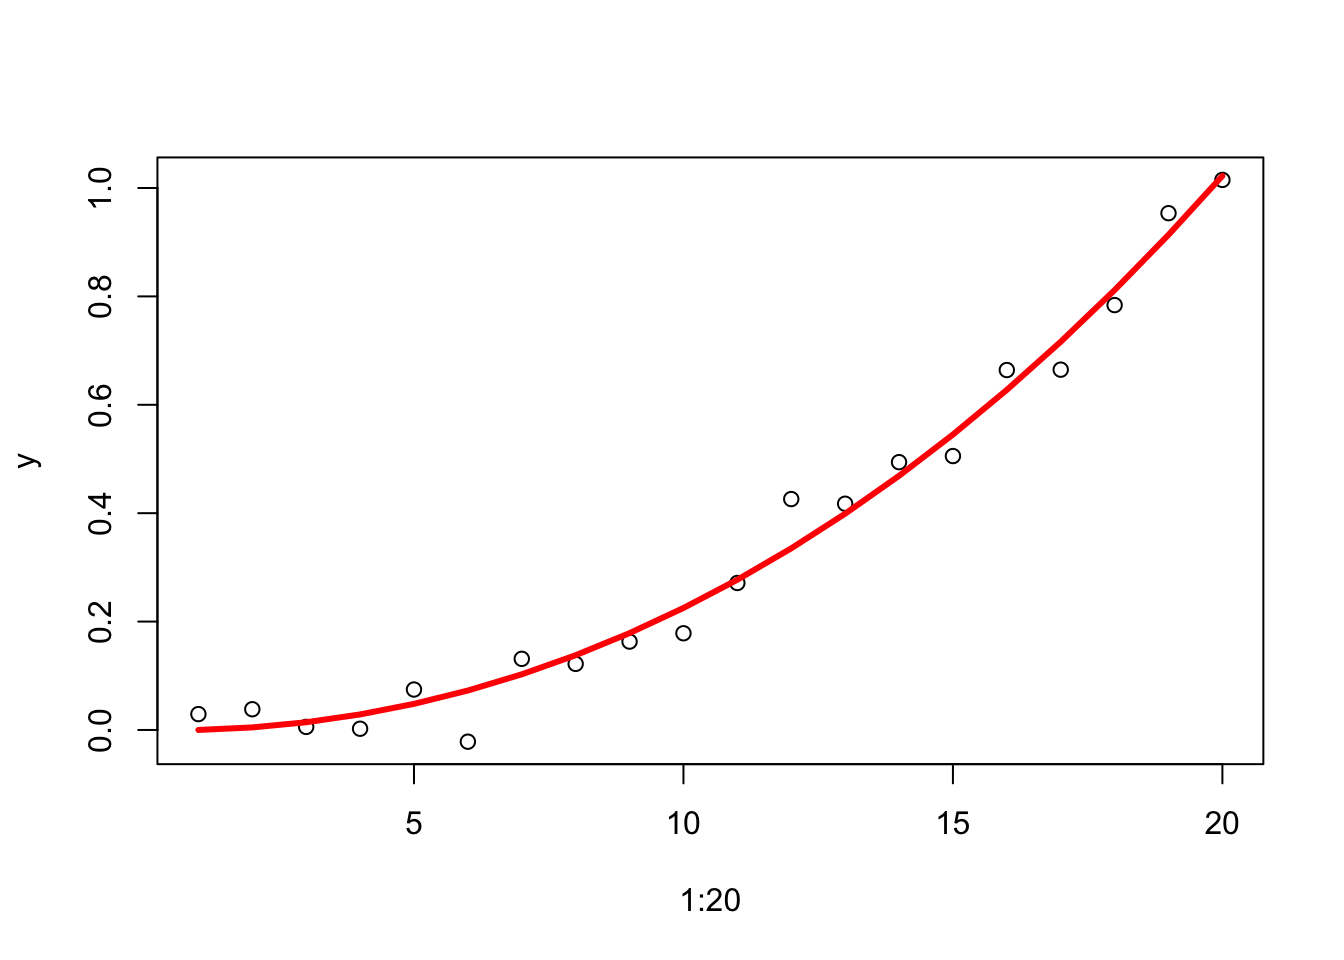
\includegraphics{polynomial_files/figure-pdf/qpmaj7-1.pdf}

The plot above and the output below shows what qpmaj() does in this
case.

\begin{verbatim}
$x
[1] -2.311264e-03  2.292295e-03  1.895686e-05

$fprimal
[1] 0.0003265426

$fdual
[1] 0.0003265446

$ftotal
[1] 0.01655943

$predict
 [1] -1.255287e-08  4.698305e-03  1.420869e-02  2.864490e-02  4.812065e-02
 [6]  7.274970e-02  1.026458e-01  1.379226e-01  1.786940e-01  2.250737e-01
[11]  2.771753e-01  3.351127e-01  3.989996e-01  4.689497e-01  5.450767e-01
[16]  6.274945e-01  7.163167e-01  8.116571e-01  9.136294e-01  1.022347e+00

$lambda
 [1] 0.1587839 0.0000000 0.0000000 0.0000000 0.0000000 0.0000000 0.0000000
 [8] 0.0000000 0.0000000 0.0000000 0.0000000 0.0000000 0.0000000 0.0000000
[15] 0.0000000 0.0000000 0.0000000 0.0000000 0.0000000 0.0000000

$inequalities
 [1] -1.255287e-08  4.698318e-03  9.510389e-03  1.443620e-02  1.947576e-02
 [6]  2.462905e-02  2.989609e-02  3.527686e-02  4.077138e-02  4.637964e-02
[11]  5.210164e-02  5.793738e-02  6.388687e-02  6.995009e-02  7.612706e-02
[16]  8.241776e-02  8.882221e-02  9.534040e-02  1.019723e-01  1.087180e-01

$itel
[1] 97
\end{verbatim}

We now want to accomplish more or less the same thing, but using a cubic
of the form \(f(x)=x(c+bx+ax^2)\). Choosing \(a, b\) and \(c\) to be
nonnegative guarantees monotonicity (and convexity) on the positive
axis, with a root at zero. If \(b^2\geq 4ac\) then the cubic has two
additional real roots, and by AM/GM we can guarantee this by
\(b\geq a + c\). So \(a\geq 0\), \(c\geq 0\), and \(b\geq a+c\) are our
three inequalities.

\begin{Shaded}
\begin{Highlighting}[]
\NormalTok{h }\OtherTok{\textless{}{-}} \FunctionTok{cbind}\NormalTok{(}\DecValTok{1}\SpecialCharTok{:}\DecValTok{20}\NormalTok{,(}\DecValTok{1}\SpecialCharTok{:}\DecValTok{20}\NormalTok{)}\SpecialCharTok{\^{}}\DecValTok{2}\NormalTok{,(}\DecValTok{1}\SpecialCharTok{:}\DecValTok{20}\NormalTok{)}\SpecialCharTok{\^{}}\DecValTok{3}\NormalTok{)}
\NormalTok{a }\OtherTok{\textless{}{-}} \FunctionTok{matrix}\NormalTok{(}\FunctionTok{c}\NormalTok{(}\DecValTok{1}\NormalTok{,}\DecValTok{0}\NormalTok{,}\DecValTok{0}\NormalTok{,}\DecValTok{0}\NormalTok{,}\DecValTok{0}\NormalTok{,}\DecValTok{1}\NormalTok{,}\SpecialCharTok{{-}}\DecValTok{1}\NormalTok{,}\DecValTok{1}\NormalTok{,}\SpecialCharTok{{-}}\DecValTok{1}\NormalTok{), }\DecValTok{3}\NormalTok{, }\DecValTok{3}\NormalTok{, }\AttributeTok{byrow =} \ConstantTok{TRUE}\NormalTok{)}
\FunctionTok{plot}\NormalTok{(}\DecValTok{1}\SpecialCharTok{:}\DecValTok{20}\NormalTok{, y)}
\NormalTok{out}\OtherTok{\textless{}{-}}\FunctionTok{qpmaj}\NormalTok{(y,}\AttributeTok{a=}\NormalTok{a,}\AttributeTok{h=}\NormalTok{h,}\AttributeTok{verbose=}\ConstantTok{FALSE}\NormalTok{,}\AttributeTok{itmax=}\DecValTok{10000}\NormalTok{, }\AttributeTok{eps =} \FloatTok{1e{-}15}\NormalTok{)}
\FunctionTok{lines}\NormalTok{(}\DecValTok{1}\SpecialCharTok{:}\DecValTok{20}\NormalTok{,out}\SpecialCharTok{$}\NormalTok{pred,}\AttributeTok{type=}\StringTok{"l"}\NormalTok{,}\AttributeTok{lwd=}\DecValTok{3}\NormalTok{,}\AttributeTok{col=}\StringTok{"RED"}\NormalTok{)}
\end{Highlighting}
\end{Shaded}

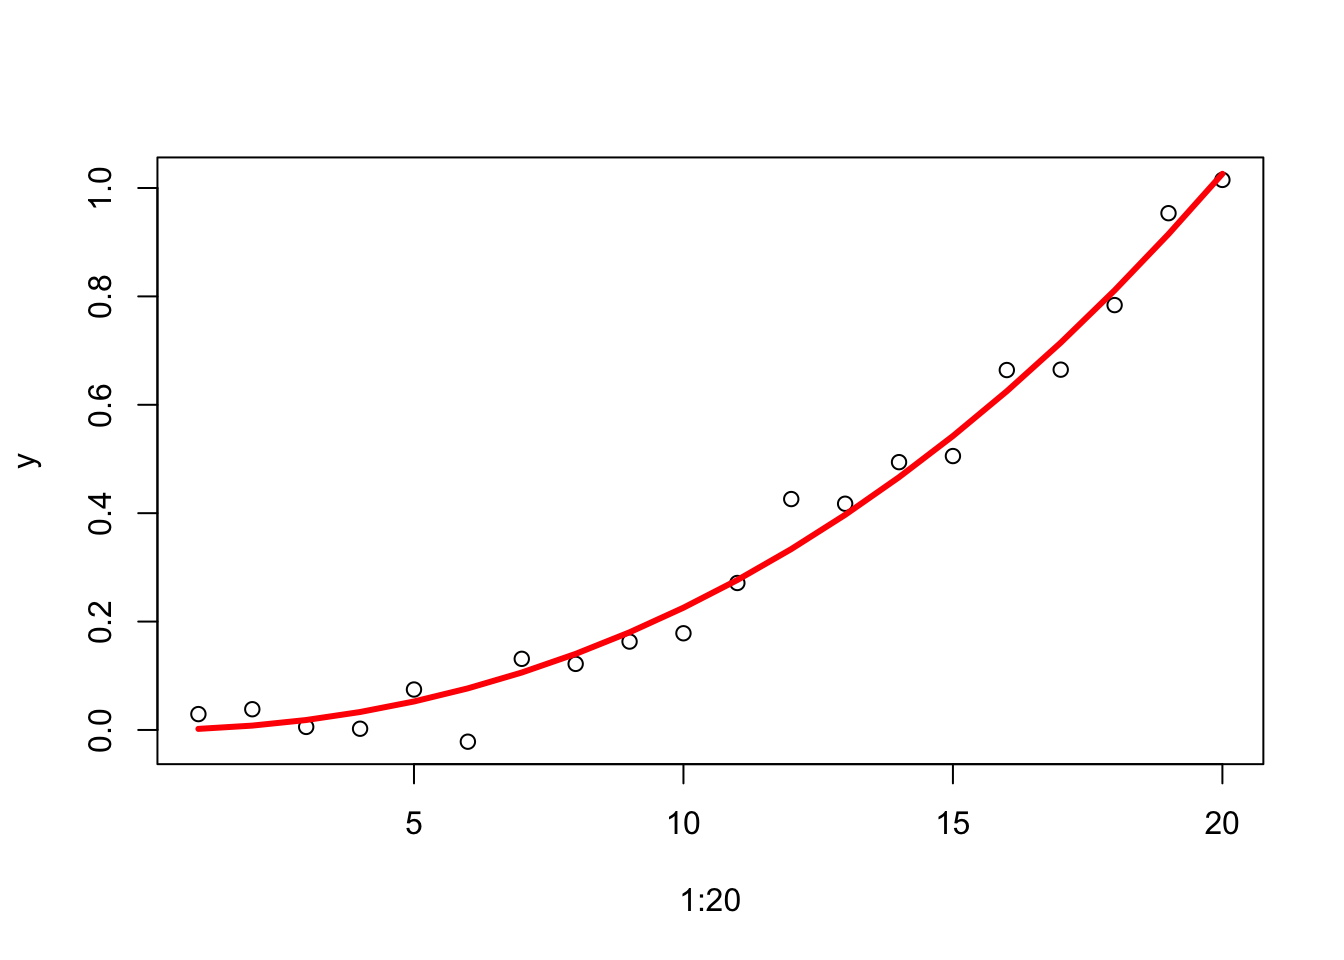
\includegraphics{polynomial_files/figure-pdf/qpmaj8-1.pdf}

The results of this alternative way of fitting the cubic are more or
less indistinguishable from the earlier results, although this second
approach is quite a bit faster (having only three inequalities instead
of 21).

\begin{verbatim}
$x
[1] -5.673813e-09  1.945808e-03  3.098195e-05

$fprimal
[1] 0.0007170899

$fdual
[1] 0.000717091

$ftotal
[1] 0.01694997

$predict
 [1] 0.001976784 0.008031075 0.018348765 0.033115745 0.052517907 0.076741142
 [7] 0.105971343 0.140394402 0.180196208 0.225562656 0.276679635 0.333733038
[13] 0.396908757 0.466392682 0.542370707 0.625028722 0.714552619 0.811128290
[19] 0.914941626 1.026178519

$lambda
[1] 0.2021458 0.0000000 0.0000000

$inequalities
[1] -5.673813e-09  3.098195e-05  1.914831e-03

$itel
[1] 25
\end{verbatim}

\subsection{Examples}\label{examples-1}

\bookmarksetup{startatroot}

\chapter{Ordinal MDS}\label{chapordinal}

\section{Monotone Regression}\label{mathmonreg}

Is it really what we want

\subsection{Simple Monotone Regression}\label{mathsimpiso}

Ever since Kruskal (\citeproc{ref-kruskal_64a}{1964a}) and Kruskal
(\citeproc{ref-kruskal_64b}{1964b}) monotone regression has played an
important part in non-metric MDS. Too important, perhaps. Initially
there was some competition with the rank images of Guttman
(\citeproc{ref-guttman_68}{1968}), but that competition has largely
faded over time.

We only give the barest outline in this section. More details are in De
Leeuw, Hornik, and Mair (\citeproc{ref-deleeuw_hornik_mair_A_09}{2009}).
In (simple least squares) monotone (or isotone) regression we minimize
\((x-y)'W(x-y)\), where \(W\gtrsim 0\) is diagonal, over \(x\)
satisfying \(x_1\leq\cdots\leq x_n\). The vector \(y\) is the
\emph{target} or the \emph{data}.

The algorithm, which is extremely fast and of order \(n\), is based on
the simple rule that if elements are out of order, then you compute
their weighted average, forming blocks, keeping track of the block sizes
and block weights. This reduces the MR problem to a smaller MR problem,
and following the rule systematically leads to a finite algorithm. A
particularly efficient implementation is in
(\citeproc{ref-busing_21}{\textbf{busing\_21?}}).

A simple illustration. The first column are the value that we compute
the best monotone fit for, the second columns are the size of the blocks
after merging. In this case there are no weights, in fact the block
sizes serve as weights.

\begin{align}
&(1,2,1,3,2,-1,3) \qquad &(1,1,1,1,1,1,1)\\
&(1,\frac32,3,2,-1,3) \qquad &(1,2,1,1,1,1)\\
&(1,\frac32,\frac52,-1,3) \qquad &(1,2,2,1,1)\\
&(1,\frac32,\frac43,3) \qquad &(1,2,3,1)\\
&(1,\frac75,3) \qquad &(1,5,1)
\end{align}

Expanding using the block size gives the solution
\((1,\frac75,\frac75,\frac75,\frac75,\frac75,3)\).

In the second example we do have weights, in the second column, and we
use a third column for blocks size.

\begin{align}
&(1,2,1,3,2,-1,3) \qquad &(1,2,3,4,3,2,1) \qquad &(1,1,1,1,1,1,1)\\
&(1,\frac75,3,2,-1,3) \qquad &(1,5,4,3,2,1) \qquad &(1,2,1,1,1,1)\\
&(1,\frac75,\frac{18}{7},-1,3) \qquad &(1,5,7,2,1) \qquad &(1,2,2,1,1)\\
&(1,\frac75,\frac{16}{9},3) \qquad &(1,5,9,1) \qquad &(1,2,3,1)
\end{align}

Expansion gives the solution
\((1,\frac75,\frac75,\frac{16}{9},\frac{16}{9},\frac{16}{9},3)\).

The usual monotone regression algorithms used in MDS allow for slightly
more complicated orders to handle ties in the data . There are basically
three approaches to ties implemented. In what Kruskal calls the
\emph{primary approach}, only order relations between tie blocks are
maintained. Within blocks no order s mposed. In the \emph{secondary
approach} we require equality in tie blocks. Ties in the data means we
impose ties in the isotone regression. Both approaches can be
incorporated in simple monotone regresson by preprocessing. The
secondary approach starts with the weighted averages of the tie blocks,
the primary approach orders the data within tie blocks so they are
non-decreasing. De Leeuw (\citeproc{ref-deleeuw_A_77}{1977b}) showed
that this preprocessing does indeed give the least squares solution for
both approaches. In the same paper he also introduces a less restrictive
\emph{tertiary approach}, which merely requires that the averages of the
tie blocks are in the required order.

\subsection{Weighted Monotone Regression}\label{mathweigmr}

\[
(x-y)'V(x-y)
\] \[V(x-y)=A'\lambda\] \[Ax\geq 0\] \[\lambda\geq 0\] \[\lambda'Ax=0\]
\[x=y+V^{-1}A'\lambda\] go to the dual if \(\lambda_i>0\) then
\(a_i'x=0\)

unweighting actually proves weighted is unweighted for something else

\(MR(x+\epsilon y)=MR(x)+\epsilon B(y)\) if \(MR(x)=Bx\)

\subsection{Normalized Cone Regression}\label{mathnorcone}

De Leeuw (\citeproc{ref-deleeuw_U_75a}{1975a})

Bauschke, Bui, and Wang (\citeproc{ref-bauschke_bui_wang_18}{2018})

\subsection{Iterative MR}\label{iterative-mr}

primal-dual: MR is dual Dykstra vertices of cone plus CCA one iteration
only

\section{Alternating Least Squares}\label{nmdsals}

smacof: hard squeeze double phase

\section{Kruskal's Approach}\label{nmdskruskal}

\subsection{Kruskal's Stress}\label{kruskals-stress-2}

Remember that Kruskal's definition of stress was intended for ordinal
multidimensional scaling only. Thus dissimilarities are not necessarily
numerical, as in basic MDS, only their rank order is known. He first
defined \emph{raw stress} as

\begin{equation}
\sigma^\star_K(X):=\mathop{\sum\sum}_{1\leq i<j\leq n} (\hat d_{ij}-d_{ij}(X))^2,
(\#eq:rawstress1)
\end{equation}

where the \(\hat d_{ij}\) is some set of numbers monotone with the
dissimilarities.

\begin{quote}
To simplify the discussion, we delay the precise definition of
\(\hat d\), for a little while. (Kruskal
(\citeproc{ref-kruskal_64a}{1964a}), p.~8)
\end{quote}

Kruskal then mentions that raw stress satisfies
\(\sigma^\star_K(\alpha X)=\alpha^2\sigma^\star_K(X)\), which is clearly
undesirable because the size of the configuration should not influence
the quality of the fit.

\begin{quote}
An obvious way to cure this defect in the raw stress is to divide it by
a scaling factor, that is, a quantity which has the same quadratic
dependence on the scale of the configuration that raw stress does.
(Kruskal (\citeproc{ref-kruskal_64a}{1964a}), p.~8).
\end{quote}

By the way, although the precise definition of \(\hat D\) has been
delayed, the uniform stretching/shrinking argument already assumes that
if we multiply \(D\) by \(\alpha\) then \(\hat D\) also gets multiplied
by \(\alpha\). Thus it sort of gives away that \(\hat D\) is also a
function of \(X\), at least of the scale of \(X\).

For the normalization of raw stress Kruskal chooses

\begin{equation}
\tau^\star_K(X):=\mathop{\sum\sum}_{1\leq i<j\leq n} d_{ij}^2(X),
(\#eq:rawtau)
\end{equation}

\begin{quote}
Finally, it is desirable to use the square root of this expression,
which is analogous to choosing the standard deviation in place of the
variance. (Kruskal (\citeproc{ref-kruskal_64a}{1964a}), p.~9)
\end{quote}

Thus Kruskal's normalized loss function for ordinal MDS becomes

\begin{equation}
\sigma_K(X):=\sqrt{\frac{\sigma^\star_K(X)}{\tau^\star_K(X)}}=\sqrt{\frac{\mathop{\sum\sum}_{1\leq i<j\leq n} (\hat d_{ij}-d_{ij}(X))^2}{\mathop{\sum\sum}_{1\leq i<j\leq n} d_{ij}^2(X)}}.
(\#eq:kruskalstress)
\end{equation}

At this point in Kruskal (\citeproc{ref-kruskal_64a}{1964a}) the
definition of \(\hat D\) still hangs in the air, although we know that
the \(\hat D\) are monotone with \(\Delta\), and that multiplying \(X\)
by a constant will multiply both \(D(X)\) and \(\hat D\) by the same
constant. Matters are clarified right after the definition of stress.

\begin{quote}
Now it is easy to define the \(\hat d_{ij}\). They are the numbers which
minimize \(\sigma\) (or equivalently, \(\sigma^\star\)) subject to the
monotonicity constraints. (Kruskal (\citeproc{ref-kruskal_64a}{1964a}),
p.~9)
\end{quote}

Thus, actually, raw stress is the minimum over the pseudo-distance
matrices \(\Omega\) in \(\mathfrak{D}\), the set of all monotone
transformations of the dissimilarities.

\begin{equation}
\sigma^\star(X):=\min_{\Omega\in\mathfrak{D}}\mathop{\sum\sum}_{1\leq i<j\leq n} (\omega_{ij}-d_{ij}(X))^2,
(\#eq:rawstressfinal)
\end{equation}

and \(\hat D\) is the minimizer, which is now clearly a function of
\(X\),

\begin{equation}
\hat D(X):=\mathop{\text{argmin}}_{\Omega\in\mathfrak{D}}\mathop{\sum\sum}_{1\leq i<j\leq n} (\omega_{ij}-d_{ij}(X))^2.
(\#eq:dhatdef)
\end{equation}

So, finally,

\begin{equation}
\sigma(X):=\min_{\Omega\in\mathfrak{D}}\sqrt{\frac{\sigma^\star(X)}{\tau^\star(X)}}=\sqrt{\frac{\mathop{\sum\sum}_{1\leq i<j\leq n} (\omega_{ij}-d_{ij}(X))^2}{\mathop{\sum\sum}_{1\leq i<j\leq n} d_{ij}^2(X)}}.
(\#eq:kruskalstressfinal)
\end{equation}

In Guttman's terminology Kruskal's approach is hard squeeze single
phase. Thus what is minimized is

\[
\sigma_{JBK}^{\ }(X):=\min_{ \Delta\in\mathfrak{D}}\sqrt{\frac{\mathop{\sum\sum}_{1\leq i<j\leq n}(\delta_{ij}-d_{ij}(X))^2}{\mathop{\sum\sum}_{1\leq i<j\leq n}d_{ij}^2(X)}}
\]

\subsection{Stress1 and Stress2}\label{stress1-and-stress2}

\section{Guttman's Approach}\label{nmdsguttman}

The main alternative to the Kruskal approach to MDS, besides smacof, is
the Smallest Space Analysis (SSA) of Guttman and Lingoes. I have mixed
feelings about the fundamental SSA paper of Guttman
(\citeproc{ref-guttman_68}{1968}). It is, no doubt, a milestone MDS
paper, and some of the distinctions it makes (which we will discuss
later in this section) are clearly important. Its use of matrix algebra,
wherever possible, is an improvement over Kruskal
(\citeproc{ref-kruskal_64a}{1964a}), and the correction matrix algorithm
for SSA is an immediate predecessor of smacof. But it seems to me the
derivation of the correction matrix algorithm is incomplete and could
even be called incorrect. The rank images used by Guttman and Lingoes in
SSA seem an ad-hoc solution invented by someone who did not yet know
about monotone regression. And, above all, the paper exudes a
personality cult-like atmosphere that is somewhat repellent to me. There
are no gurus in science. Or at least there should not be. It is true
that between 1930 and 1960 Guttman invented and elucidated about 75\% of
the psychometrics of his time, but 75\% is still less than 100\%. This
book you are reading now may set a record in self-citation, but that
makes sense because it is supposed to document my work in MDS and to
give access to the pdf's of my unpublished work. I try to be careful not
to take credit for results that did not originate with me, and to give
appropriate attributions in all cases.

\subsubsection{Rank Images}\label{rank-images}

The rank image transformation, which replaces the monotone regression in
Kruskal's approach, has a rather complicated definition. It is simple
enough when both \(\Delta\) and \(D(X)\) have no ties. In that case the
rank image \(D^\star\) is just the unique permutation of \(D(X)\) that
is monotone with \(\Delta\). Thus

\begin{equation}
\delta_{ij}<\delta_{kl}\Leftrightarrow d_{ij}^\star<d_{kl}^\star.
(\#eq:nmrankimage0)
\end{equation}

If there are ties in \(\Delta\) and/or \(D(X)\) then some of the
uniqueness and simplicity will get lost. Guttman
(\citeproc{ref-guttman_68}{1968}) introduces an elaborate notation for
rank images with ties, but that notation does neither him nor the reader
any favors.

If there are ties in \(D(X)\) you use the rank order of the
corresponding elements of \(\Delta\) to order \(D(X)\) within tie
blocks. If two elements are tied both in \(D(X)\) and \(\Delta\), then
their order in the tie block is arbitrary.

Suppose the \(\Delta\) have \(R\) tie-blocks, in increasing order, with
\(m_1,\cdots,m_R\) elements. The smallest \(m_1\) elements of the vector
of distances become the first \(m_1\) elements of \(D^\star\), the next
\(m_2\) elements of \(D^\star\) are the next smallest \(m^2\) elements
of distance vector, and so on for all tie blocks. Thus tied elements in
\(\Delta\) can become untied in \(D^\star\) and untied elements in
\(\Delta\) can becomes tied in \(D^\star\). We require

\begin{equation}
\delta_{ij}<\delta_{kl}\Rightarrow d_{ij}^\star\leq d_{kl}^\star
(\#eq:nmrankimage1)
\end{equation}

This corresponds with Kruskal's primary approach to ties. Guttman calls
it \emph{semi-strong monotonicity}. There is a small numerical example
in table @ref(tab:nmriexample1).

\begin{longtable}[]{@{}lrrrrrrr@{}}
\caption{Semi-strong Rank Images}\tabularnewline
\toprule\noalign{}
& 1 & 2 & 3 & 4 & 5 & 6 & 7 \\
\midrule\noalign{}
\endfirsthead
\toprule\noalign{}
& 1 & 2 & 3 & 4 & 5 & 6 & 7 \\
\midrule\noalign{}
\endhead
\bottomrule\noalign{}
\endlastfoot
\(\Delta\) & 1 & 2 & 2 & 3 & 3 & 4 & 5 \\
\(D(X)\) & 1 & 3 & 1 & 3 & 4 & 3 & 4 \\
\(D(X)\ \text{ordered}\) & 1 & 1 & 3 & 3 & 3 & 4 & 4 \\
\(D^\star\) & 1 & 1 & 3 & 3 & 3 & 4 & 4 \\
\end{longtable}

The sum of the squared differences between \(D(X)\) and \(D^\star\) is
6.

Alternatively, we can require that tied elements in \(\Delta\)
correspond with tied elements in \(D^\star\). Guttman calls this
\emph{strong monotonicity}, and requires in addition that \(D^\star\)
has the same number of blocks, with the same block sizes, as \(\Delta\).
Instead of copying ordered blocks from the sorted distances, we compute
averages of blocks, and copy those into \(D^star\). This corresponds
with Kruskal's secondary approach to ties. Thus the elements of
\(D^\star\) are no longer a permutation of those in \(D(X)\). We have
@eq:nmrankimage1, and also

\begin{equation}
\delta_{ij}=\delta_{kl}\Rightarrow d_{ij}^\star=d_{kl}^\star
(\#eq:nmrankimage2)
\end{equation}

Our numerical example is now in table @ref(tab:nmriexample2).

\begin{longtable}[]{@{}lrrrrrrr@{}}
\caption{Strong Rank Images}\tabularnewline
\toprule\noalign{}
& 1 & 2 & 3 & 4 & 5 & 6 & 7 \\
\midrule\noalign{}
\endfirsthead
\toprule\noalign{}
& 1 & 2 & 3 & 4 & 5 & 6 & 7 \\
\midrule\noalign{}
\endhead
\bottomrule\noalign{}
\endlastfoot
\(\Delta\) & 1 & 2 & 2 & 3 & 3 & 4 & 5 \\
\(D(X)\) & 1 & 3 & 1 & 3 & 4 & 3 & 4 \\
\(D(X)\ \text{ordered}\) & 1 & 1 & 3 & 3 & 3 & 4 & 4 \\
\(D^\star\) & 1 & 2 & 2 & 3 & 3 & 4 & 4 \\
\end{longtable}

Now the sum of squared differences between \(D(X)\) and \(D^\star\) is
4, which means, surprisingly, that strong monotonicity gives a better
fit than semi-strong monotonicity. This cannot happen with monotone
regression, where the primary approch to ties always has a better fit
than the secondary approach.

\subsubsection{Single and Double Phase}\label{single-and-double-phase}

Note: suppose \(\|D_1^\star-D(X_2)\|^2<\|D_1^\star-D(X_1)\|^2\) but
\(\|D_2^\star-D(X_2)\|^2>\|D_1^\star-D(X_2)\|^2\)

\[
\sigma_G(X)=\frac{\mathop{\sum\sum}_{1\leq i<j\leq n}w_{ij}(d^\star_{ij}(X)-d_{ij}(X))^2}{\mathop{\sum\sum}_{1\leq i<j\leq n}w_{ij}d_{ij}^2(X)}.
\]

\[
\sigma_G(X,D^\star)=\frac{\mathop{\sum\sum}_{1\leq i<j\leq n}(d^\star_{ij}-d_{ij}(X))^2}{\mathop{\sum\sum}_{1\leq i<j\leq n}d_{ij}^2(X)}.
\]

\subsubsection{Hard and Soft Squeeze}\label{hard-and-soft-squeeze}

\[
\sigma(X):=\min_{\delta\in\mathbb{K}\cap\mathbb{S}}\sum_{k\in\mathcal{K}}w_k(\delta_k-d_k(X))^2
\]

question: in double phase do rank images decrease stress ? My guess is
yes. Are they continuous ?

\[\rho_G(X)=\max_{P\in\Pi} \delta'Pd(X)\] is a continuous function of
\(X\). Also (Shepard) \[
D_+\rho_G(X)=\max_{P\in\Pi(X)}\delta'P\mathcal{D}d(X)
\]

rank-images \(Pd\) are not continuous

\subsection{Smoothness of Ordinal Loss
Functions}\label{smoothness-of-ordinal-loss-functions}

Kruskal

\[
\min_{\hat D\in\mathfrak{D}}\sum\sum w_{ij}(\hat d_{ij}-d_{ij}(X))^2
\] is a differentiable function of \(X\)

Double phase rank image

\[
\sigma_{LG}(X)=\min_P\|Pd(X)-d(X)\|^2
\] \(P\) in the Birkhoff polytope and satisfying inequalities,
equalities.

\(P\) given by \(\max_P d(X)'Pd(X)\)

De Leeuw (\citeproc{ref-deleeuw_R_73g}{1973b})

\section{Scaling with Distance
Bounds}\label{scaling-with-distance-bounds}

\[
\alpha_{ij}\leq d_{ij}(X)\leq\beta_{ij}
\]

\section{Bounds on Stress}\label{bounds-on-stress}

De Leeuw and Stoop (\citeproc{ref-deleeuw_stoop_A_84}{1984})

Stress1 and Stress2

\bookmarksetup{startatroot}

\chapter{Splinical MDS}\label{chsplinical}

\section{Splines}\label{mathsplines}

In this section we give a short introduction, with examples, to
(univariate) splines, B-splines, and I-splines. It is taken from De
Leeuw (\citeproc{ref-deleeuw_E_17i}{2017a}), with some edits to make it
fit into the book. The report it was taken from has more detail and more
examples.

To define \emph{spline functions} we first define a finite sequence of
\emph{knots} \(T=\{t_j\}\) on the real line, with
\(t_1\leq\cdots\leq t_p,\) and an \emph{order} \(m\). In addition each
knot \(t_j\) has a \emph{multiplicity} \(m_j\), the number of knots
equal to \(t_j\). We suppose throughout that \(m_j\leq m\) for all
\(j\).

A function \(f\) is a \emph{spline function of order} \(m\) for a knot
sequence \(\{t_j\}\) if

\begin{enumerate}
\def\labelenumi{\arabic{enumi}.}
\tightlist
\item
  \(f\) is a polynomial \(\pi_j\) of degree at most \(m-1\) on each
  half-open interval \(I_j=[t_j,t_{j+1})\) for \(j=1,\cdots,p\),
\item
  the polynomial pieces are joined in such a way that
  \(\mathcal{D}^{(s)}_-f(t_j)=\mathcal{D}^{(s)}_+f(t_j)\) for
  \(s=0,1,\cdots,m-m_j-1\) and \(j=1,2,\cdots,p\).
\end{enumerate}

Here we use \(\mathcal{D}^{(s)}_-\) and \(\mathcal{D}^{(s)}_+\) for the
left and right \(s^{th}\)-derivative operator. If \(m_j=m\) for some
\(j\), then the second requirement is empty, if \(m_j=m-1\) then the
second requirement means \(\pi_j(t_j)=\pi_{j+1}(t_j)\), i.e.~we require
continuity of \(f\) at \(t_j\). If \(1\leq m_j<m-1\) then \(f\) must be
\(m-m_j-1\) times differentiable, and thus continuously differentiable,
at \(t_j\).

In the case of simple knots (with multiplicity one) a spline function of
order one is a \emph{step function} which steps from one level to the
next at each knot. A spline of order two is piecewise linear, with the
pieces joined at the knots so that the spline function is continuous.
Order three means a piecewise quadratic function which is continuously
differentiable at the knots. And so on.

\subsection{B-splines}\label{mathbsplines}

Alternatively, a spline function of order \(m\) can be defined as a
linear combination of \emph{B-splines} (or \emph{basic splines}) of
order \(m\) on the same knot sequence. A B-spline of order \(m\) is a
spline function consisting of at most \(m\) non-zero polynomial pieces.
A B-spline \(\mathcal{B}_{j,m}\) is determined by the \(m+1\) knots
\(t_j\leq\cdots\leq t_{j+m}\), is zero outside the interval
\([t_j,t_{j+m})\), and positive in the interior of that interval. Thus
if \(t_j=t_{j+m}\) then \(\mathcal{B}_{j,m}\) is identically zero.

For an arbitrary finite knot sequence \(t_1,\cdots,t_p\), there are
\(p-m\) B-splines to of order \(m\) to be considered, although some may
be identically zero. Each of the splines covers at most \(m\)
consecutive intervals, and at most \(m-1\) different B-splines are
non-zero at each point.

\subsubsection{Boundaries}\label{mathbboundaries}

B-splines are most naturally and simply defined for doubly infinite
sequences of knots, that go to \(\pm\infty\) in both directions. In that
case we do not have to worry about boundary effects, and each
subsequence of \(m+1\) knots defines a B-spline. For splines on finite
sequences of \(p\) knots we have to decide what happens at the boundary
points.

There are B-splines for \(t_j,\cdots,t_{j+m}\) for all
\(j=1,\cdots,p-m\). This means that the first \(m-1\) and the last
\(m-1\) intervals have fewer than \(m\) splines defined on them. They
are not part of what De Boor (\citeproc{ref-deboor_01}{2001}), page 94,
calls the \emph{basic interval}. For doubly infinite sequences of knots
there is not need to consider such a basic interval.

If we had \(m\) additional knots on both sides of our knot sequence we
would also have \(m\) additional B-splines for \(j=1-m,\cdots,0\) and
\(m\) additional B-splines for \(j=p-m+1,\cdots,p\). By adding these
additional knots we make sure each interval \([t_j,t_{j+1})\) for
\(j=1,\cdots,p-1\) has \(m\) B-splines associated with it. There is stil
some ambiguity on what to do at \(t_p\), but we can decide to set the
value of the spline there equal to the limit from the left, thus making
the B-spline left-continuous there.

In our software we will use the convention to define our splines on a
closed interval \([a,b]\) with \(r\) \emph{interior knots}
\(a<t_1<\cdots<t_r<b\), where interior knot \(t_j\) has multiplicity
\(m_j\). We extend this to a series of \(p=M+2m\) knots, with
\(M=\sum_{j=1}^r m_j\), by starting with \(m\) copies of \(a\),
appending \(m_j\) copies of \(t_j\) for each \(j=1,\cdots,r\), and
finishing with \(m\) copies of \(b\). Thus \(a\) and \(b\) are both
knots with multiplicity \(m\). This defines the \emph{extended
partition} (Schumaker (\citeproc{ref-schumaker_07}{2007}), p 116), which
is just handled as any knot sequence would normally be.

\subsubsection{Normalization}\label{mathbnormalize}

The conditions we have mentioned only determine the B-spline up to a
normalization. There are two popular ways of normalizing B-splines. The
\(N\)-splines \(N_{j,m}\), a.k.a. the \emph{normalized B-splines} \(j\)
or order \(m\), satisfies \begin{equation}\label{E:nsum}
\sum_{j}N_{j,m}(t)=1.
\end{equation} Note that in general this is not true for all \(t\), but
only for all \(t\) in the \emph{basic interval}.

Alternatively we can normalize to \(M\)-splines, for which
\begin{equation}\label{E:mint}
\int_{-\infty}^{+\infty}M_{j,m}(t)dt=\int_{t_j}^{t_{j+k}}M_{j,m}(t)dt=1.
\end{equation} There is the simple relationship
\begin{equation}\label{E:NM}
N_{j,m}(t)=\frac{t_{j+m}-t_j}{m}\ M_{j,m}(t).
\end{equation}

\subsubsection{Recursion}\label{mathbrecursion}

B-splines can be defined in various ways, using piecewise polynomials,
divided differences, or recursion. The recursive definition, first used
as the preferred definition of B-splines by De Boor and Höllig
(\citeproc{ref-deboor_hollig_85}{1985}), is the most convenient one for
computational purposes, and that is the one we use.

The recursion is due independently to M. G. Cox
(\citeproc{ref-cox_72}{1972}) for simple knots and to De Boor
(\citeproc{ref-deboor_72}{1972}) in the general case, is
\begin{equation}\label{E:Mspline}
M_{j,m}(t)=\frac{t-t_j}{t_{j+m}-t_j}M_{j,m-1}(t)+\frac{t_{j+m}-t}{t_{j+m}-t_j}M_{j+1,m-1}(t),
\end{equation} or \begin{equation}\label{E:Nspline}
N_{j,m}(t)=\frac{t-t_j}{t_{m+j-1}-t_j}N_{j,m-1}(t)+\frac{t_{j+m}-t}{t_{j+m}-t_{j+1}}N_{j+1,m-1}(t).
\end{equation}

A basic result in the theory of B-splines is that the different
B-splines are linearly independent and form a basis for the linear space
of spline functions (of a given order and knot sequence).

In section @ref(apcodemathadd) the basic BSPLVB algorithm from De Boor
(\citeproc{ref-deboor_01}{2001}), page 111, for normalized B-splines is
translated to R and C. There are two auxiliary routines, one to create
the extended partition, and one that uses bisection to locate the knot
interval in which a particular value is located (Schumaker
(\citeproc{ref-schumaker_07}{2007}), p 191). The R function
bsplineBasis() takes an arbitrary knot sequence. It can be combined with
extendPartition(), which uses inner knots and boundary points to create
the extended partion.

\subsubsection{Illustrations}\label{illustrations}

For our example, which is the same as the one from figure 1 in Ramsay
(\citeproc{ref-ramsay_88}{1988}), we choose \(a=0\), \(b=1\), with
simple interior knots 0.3, 0.5, 0.6. First the \emph{step functions},
which have order 1.

\begin{figure}[H]

{\centering 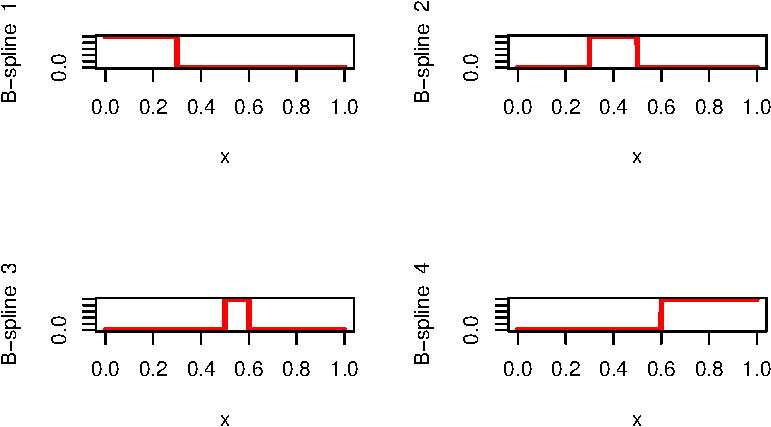
\includegraphics{splinical_files/figure-pdf/order1mult1-1.pdf}

}

\caption{Zero Degree Splines with Simple Knots}

\end{figure}%

Now the \emph{hat functions}, which have order 2, again with simple
knots.

\begin{figure}[H]

{\centering 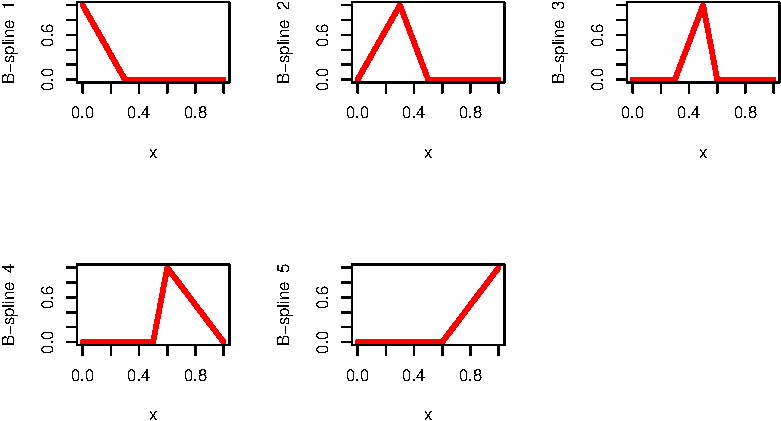
\includegraphics{splinical_files/figure-pdf/order2mult1-1.pdf}

}

\caption{Piecewise Linear Splines with Simple Knots}

\end{figure}%

Next piecewise quadratics, with simple knots, which implies continuous
differentiability at the knots. This are the N-splines corresponding
with the M-splines in figure 1 of Ramsay
(\citeproc{ref-ramsay_88}{1988}).

\begin{figure}[H]

{\centering 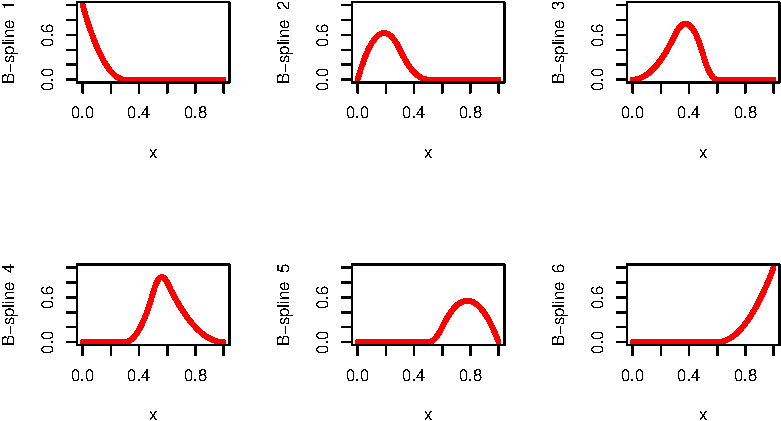
\includegraphics{splinical_files/figure-pdf/order3mult1-1.pdf}

}

\caption{Piecwise Quadratic Splines with Simple Knots}

\end{figure}%

If we change the multiplicities to 1, 2, 3, then we lose some of the
smoothness.

\subsection{I-splines}\label{mathisplines}

There are several ways to require splines to be monotone increasing.
Since B-splines are non-negative, the definite integral of a B-spline of
order \(m\) from the beginning of the interval to a value \(x\) in the
interval is an increasing spline of order \(m+1\). Integrated B-splines
are known as \emph{I-splines} (Ramsay (\citeproc{ref-ramsay_88}{1988})).
Non-negative linear combinations I-splines can be used as a basis for
the convex cone of increasing splines. Note, however, that if we use an
extended partition, then all I-splines start at value zero and end at
value one, which means their convex combinations are those splines that
are also probability distributions on the interval. To get a basis for
the increasing splines we need to add the constant function to the
I-splines and allow it to enter the linear combination with either sign.

I-splines are most economically computed by using the formula first
given by Gaffney (\citeproc{ref-gaffney_76}{1976}). If \(\ell\) is
defined by \(t_{j+\ell-1}\leq x<t_{j+\ell}\) then \[
\int_{x_j}^x M_{j,m}(t)dt=\frac{1}{m}\sum_{r=0}^{ \ell-1}(x-x_{j+r})M_{j+r,m-r}(x)
\] It is somewhat simpler, however, to use lemma 2.1 of De Boor, Lyche,
and Schumaker (\citeproc{ref-deboor_lyche_schumaker_76}{1976}). This
says \[
\int_a^xM_{j,m}(t)dt=\sum_{\ell\geq j}N_{\ell,m+1}(x)-\sum_{\ell\geq j}N_{\ell,m+1}(a),
\] If we specialize this to I-splines, we find , as in De Boor
(\citeproc{ref-deboor_76}{1976}), formula 4.11, \[
\int_{-\infty}^x M_{j,m}(t)dt=\sum_{\ell=j}^{j+r}N_{\ell,m+1}(x)
\] for \(x\leq t_{j+r+1}\). This shows that I-splines can be computed by
using cumulative sums of B-spline values.

Note that using the definition using integration does not give a natural
way to define increasing splines of degree one, i.e.~increasing step
functions. There is no such problem with the cumulative sum approach.

\subsubsection{Increasing Coefficients}\label{increasing-coefficients}

As we know, a spline is a linear combination of B-splines. The formula
for the derivative of a spline, for example in De Boor
(\citeproc{ref-deboor_01}{2001}), p 116, shows that a spline is
increasing if the coefficients of the linear combination of B-splines
are increasing. Thus we can fit an increasing spline by restricting the
coefficients of the linear combination to be increasing, again using the
B-spline basis.

It turns out this is in fact identical to using I-splines. If the
B-spline values at \(n\) points are in an \(n\times r\) matrix \(H\),
then non-decreasing coefficients \(\beta\) are of the form
\(\beta=S\alpha+\gamma e_r\), where \(S\) is lower-diagonal with all
elements on and below the diagonal equal to one, where \(\alpha\geq 0\),
where \(e_r\) has all elements equal to one, and where \(\gamma\) can be
of any sign. So \(H\beta=(HS)\alpha+\gamma e_n\). Thus non-decreasing
coefficients is the same thing as using cumnulative sums of the B-spline
basis.

\subsubsection{Increasing Values}\label{increasing-values}

Finally, we can simply require that the \(n\) elements of \(H\beta\) are
increasing. This is a less restrictive requirement, because it allows
for the possibility that the spline is decreasing between data values.
It has the rather serious disadvantage, however, that it does its
computations in \(n\)-dimensional space, and not in \(r\)-dimensional
space, where \(r=M+m\), which is usually much smaller than \(n\).
Software for the increasing-value restrictions has been written by De
Leeuw (\citeproc{ref-deleeuw_E_15e}{2015}). In our software, however, we
prefer the \texttt{cumsum()} approach. It is less general, but
considerably more efficient.

We use the same Ramsay example as before, but now cumulatively. First we
integrate step functions with simple knots, which have order one, using
\texttt{isplineBasis()}. The corresponding I-splines are piecewise
linear with order two.

\begin{figure}[H]

{\centering 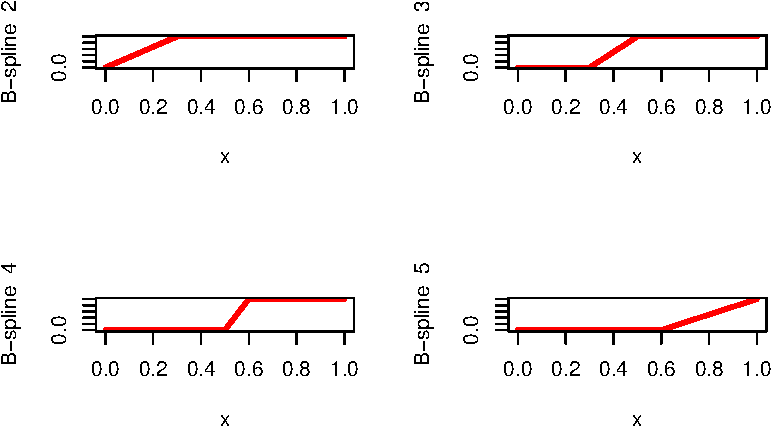
\includegraphics{splinical_files/figure-pdf/Iorder1mult1-1.pdf}

}

\caption{Not Sure}

\end{figure}%

Now we integrate the hat functions, which have order 2, again with
simple knots, to find piecewise quadratic I-splines of order 3. These
are the functions in the example of Ramsay
(\citeproc{ref-ramsay_88}{1988}).

\begin{figure}[H]

{\centering 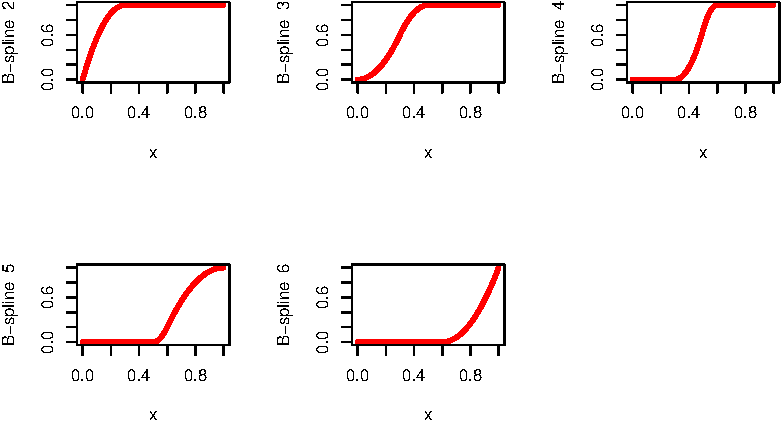
\includegraphics{splinical_files/figure-pdf/Iorder2mult1-1.pdf}

}

\caption{Monotone Piecewise Linear Splines with Simple Knots}

\end{figure}%

Finally, we change the multiplicities to 1, 2, 3, and compute the
corresponding piecewise quadratic I-splines.

\subsection{Time Series Example}\label{time-series-example}

Our first example smoothes a time series by fitting a spline. We use the
number of births in New York from 1946 to 1959 (on an unknown scale),
from Rob Hyndman's time series archive.

\subsubsection{B-splines}\label{b-splines}

First we fit B-splines of order three. The basis matrix uses \(x\) equal
to \(1:168\), with inner knots 12, 24, 36, 48, 60, 72, 84, 96, 108, 120,
132, 144, 156, and interval \([1,168]\).

\begin{Shaded}
\begin{Highlighting}[]
\NormalTok{innerknots }\OtherTok{\textless{}{-}} \DecValTok{12} \SpecialCharTok{*} \DecValTok{1}\SpecialCharTok{:}\DecValTok{13}
\NormalTok{multiplicities }\OtherTok{\textless{}{-}} \FunctionTok{rep}\NormalTok{(}\DecValTok{1}\NormalTok{, }\DecValTok{13}\NormalTok{)}
\NormalTok{lowend }\OtherTok{\textless{}{-}} \DecValTok{1}
\NormalTok{highend }\OtherTok{\textless{}{-}} \DecValTok{168}
\NormalTok{order }\OtherTok{\textless{}{-}} \DecValTok{3}
\NormalTok{x }\OtherTok{\textless{}{-}} \DecValTok{1}\SpecialCharTok{:}\DecValTok{168}
\NormalTok{knots }\OtherTok{\textless{}{-}}
  \FunctionTok{extendPartition}\NormalTok{ (innerknots, multiplicities, order, lowend, highend)}\SpecialCharTok{$}\NormalTok{knots}
\NormalTok{h }\OtherTok{\textless{}{-}} \FunctionTok{bsplineBasis}\NormalTok{ (x, knots, order)}
\NormalTok{u }\OtherTok{\textless{}{-}} \FunctionTok{lm.fit}\NormalTok{(h, births)}
\NormalTok{res }\OtherTok{\textless{}{-}} \FunctionTok{sum}\NormalTok{ ((births }\SpecialCharTok{{-}}\NormalTok{ h }\SpecialCharTok{\%*\%}\NormalTok{ u}\SpecialCharTok{$}\NormalTok{coefficients) }\SpecialCharTok{\^{}} \DecValTok{2}\NormalTok{) }\SpecialCharTok{/} \DecValTok{2}
\end{Highlighting}
\end{Shaded}

\begin{figure}[H]

{\centering 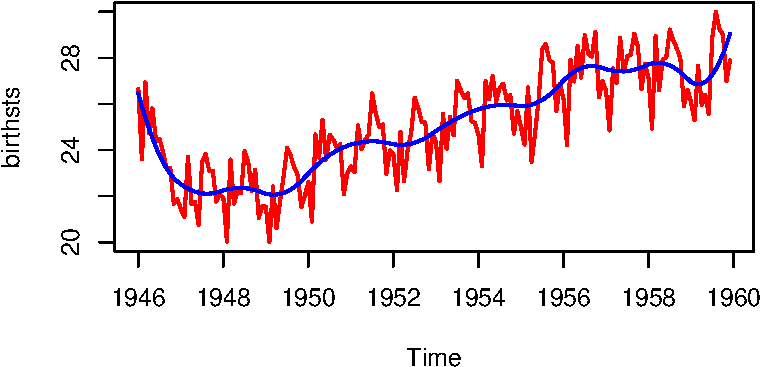
\includegraphics{splinical_files/figure-pdf/birthbsplineplot-1.pdf}

}

\caption{Monotone Piecewise Quadratic Splines with Simple Knots}

\end{figure}%

The residual sum of squares is 114.6917709.

\subsubsection{I-splines}\label{i-splines}

We now fit the I-spline using the B-spline basis. Compute \(Z=HS\) using
\texttt{cumsum()}, and then \(\overline y\) and \(\overline Z\) by
centering (substracting the column means). The formula is \[
\min_{\alpha\geq 0,\gamma}\mathbf{SSQ}\ (y-Z\alpha-\gamma e_n)=\min_{\alpha\geq 0}\mathbf{SSQ}\ (\overline y-\overline Z\alpha).
\] We use \texttt{pnnls()} from Wang, Lawson, and Hanson
(\citeproc{ref-wang_lawson_hanson_15}{2015}).

\begin{Shaded}
\begin{Highlighting}[]
\NormalTok{knots }\OtherTok{\textless{}{-}} \FunctionTok{extendPartition}\NormalTok{ (innerknots, multiplicities, order, lowend, highend)}\SpecialCharTok{$}\NormalTok{knots}
\NormalTok{h }\OtherTok{\textless{}{-}} \FunctionTok{isplineBasis}\NormalTok{ (x, knots, order)}
\NormalTok{g }\OtherTok{\textless{}{-}} \FunctionTok{cbind}\NormalTok{ (}\DecValTok{1}\NormalTok{, h[,}\SpecialCharTok{{-}}\DecValTok{1}\NormalTok{])}
\NormalTok{u }\OtherTok{\textless{}{-}} \FunctionTok{pnnls}\NormalTok{ (g, births, }\DecValTok{1}\NormalTok{)}\SpecialCharTok{$}\NormalTok{x}
\NormalTok{v }\OtherTok{\textless{}{-}}\NormalTok{ g}\SpecialCharTok{\%*\%}\NormalTok{u}
\end{Highlighting}
\end{Shaded}

\begin{figure}[H]

{\centering 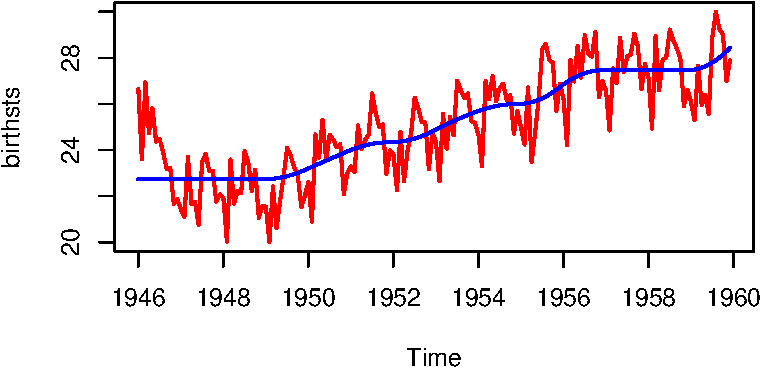
\includegraphics{splinical_files/figure-pdf/birthsisplinesplot-1.pdf}

}

\caption{Monotone Piecewise Linear Splines with Simple Knots}

\end{figure}%

The residual sum of squares is 144.2027491.

\subsubsection{B-Splines with monotone
weights}\label{b-splines-with-monotone-weights}

Just to make sure, we also solve the problem \[
\min_{\beta_1\leq\beta_2\leq\cdots\leq\beta_p}\mathbf{SSQ}(y-X\beta),
\] which should give the same solution, and the same loss function
value, because it is just another way to fit I-splines. We use the
\texttt{lsi()} function from Wang, Lawson, and Hanson
(\citeproc{ref-wang_lawson_hanson_15}{2015}).

\begin{Shaded}
\begin{Highlighting}[]
\NormalTok{knots }\OtherTok{\textless{}{-}}
  \FunctionTok{extendPartition}\NormalTok{ (innerknots, multiplicities, order, lowend, highend)}\SpecialCharTok{$}\NormalTok{knots}
\NormalTok{h }\OtherTok{\textless{}{-}} \FunctionTok{bsplineBasis}\NormalTok{ (x, knots, order)}
\NormalTok{nb }\OtherTok{\textless{}{-}} \FunctionTok{ncol}\NormalTok{ (h)}
\NormalTok{d }\OtherTok{\textless{}{-}} \FunctionTok{matrix}\NormalTok{(}\DecValTok{0}\NormalTok{, nb }\SpecialCharTok{{-}} \DecValTok{1}\NormalTok{, nb)}
\FunctionTok{diag}\NormalTok{(d) }\OtherTok{=} \SpecialCharTok{{-}}\DecValTok{1}
\NormalTok{d[}\FunctionTok{outer}\NormalTok{(}\DecValTok{1}\SpecialCharTok{:}\NormalTok{(nb }\SpecialCharTok{{-}} \DecValTok{1}\NormalTok{), }\DecValTok{1}\SpecialCharTok{:}\NormalTok{nb, }\ControlFlowTok{function}\NormalTok{(i, j)}
\NormalTok{  (j }\SpecialCharTok{{-}}\NormalTok{ i) }\SpecialCharTok{==} \DecValTok{1}\NormalTok{)] }\OtherTok{\textless{}{-}} \DecValTok{1}
\NormalTok{u }\OtherTok{\textless{}{-}} \FunctionTok{lsi}\NormalTok{(h, births, }\AttributeTok{e =}\NormalTok{ d, }\AttributeTok{f =} \FunctionTok{rep}\NormalTok{(}\DecValTok{0}\NormalTok{, nb }\SpecialCharTok{{-}} \DecValTok{1}\NormalTok{))}
\NormalTok{v }\OtherTok{\textless{}{-}}\NormalTok{ h }\SpecialCharTok{\%*\%}\NormalTok{ u}
\end{Highlighting}
\end{Shaded}

\begin{center}
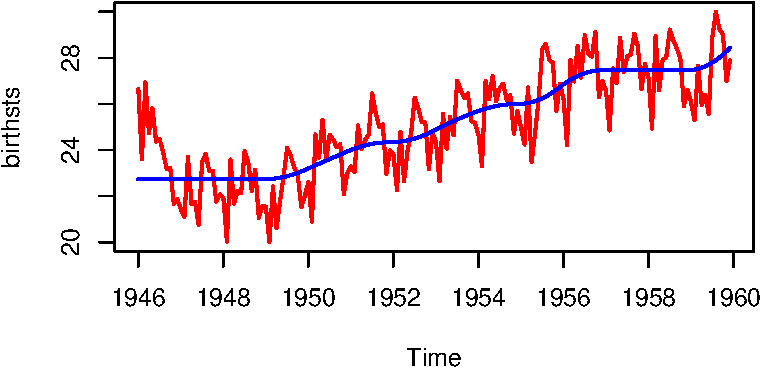
\includegraphics{splinical_files/figure-pdf/birthsisplinesvaluesplot-1.pdf}
\end{center}

The residual sum of squares is 144.2027491, indeed the same as before.

\subsubsection{B-Splines with monotone
values}\label{b-splines-with-monotone-values}

Finally we solve

\[
\min_{x_1'\beta\leq\cdots\leq x_n'\beta} \mathbf{SSQ}\ (y-X\beta)
\]

using qpmaj() from section ???.

\begin{Shaded}
\begin{Highlighting}[]
\NormalTok{knots }\OtherTok{\textless{}{-}}
  \FunctionTok{extendPartition}\NormalTok{ (innerknots, multiplicities, order, lowend, highend)}\SpecialCharTok{$}\NormalTok{knots}
\NormalTok{h }\OtherTok{\textless{}{-}} \FunctionTok{bsplineBasis}\NormalTok{ (x, knots, order)}
\NormalTok{a }\OtherTok{\textless{}{-}} \FunctionTok{diff}\NormalTok{(}\FunctionTok{diag}\NormalTok{(}\FunctionTok{nrow}\NormalTok{(h))) }\SpecialCharTok{\%*\%}\NormalTok{ h}
\NormalTok{u }\OtherTok{\textless{}{-}} \FunctionTok{qpmaj}\NormalTok{(births, }\AttributeTok{h =}\NormalTok{ h, }\AttributeTok{a =}\NormalTok{ a)}
\end{Highlighting}
\end{Shaded}

\begin{figure}[H]

{\centering 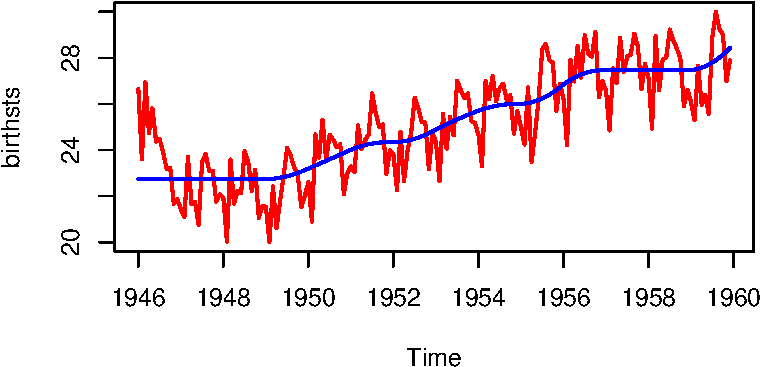
\includegraphics{splinical_files/figure-pdf/birthsbsplinesmonotonicplot-1.pdf}

}

\caption{Monotone Piecewise Quadratic Splines with Multiple Knots}

\end{figure}%

The residual sum of squares is 144.1574541 , which is indeed smaller
than the I-splines value, although only very slightly so.

\subsection{Local positivity, monotonicity,
convexity}\label{local-positivity-monotonicity-convexity}

\bookmarksetup{startatroot}

\chapter{Unidimensional Scaling}\label{unidimensional}

For Unidimensional Scaling (UDS or 1MDS) the configuration is a matrix
\(X\in\mathbb{R}^{n\times 1}\). We can trivially identify this
single-column matrix \(X\) with the vector \(x\) of coordinates of \(n\)
points on the real line. All our previous general MDS results remain
valid for UDS, but we will use the additional structure that comes with
\(p=1\) to discuss a number of special results.

Unidimensional scaling appears under different names in the literature
such as \emph{seriation} in archeology and \emph{sequencing} in
genetics. Often the algorithms permute the rows and columns of a matrix
of dissimilarities to approximate some special structure. In this book
seriation and sequencing are always understood to be the minimization of
stress over \(x\), i.e.~minimization of

\begin{equation}
\sigma(x)=\mathop{\sum\sum}_{1\leq i<j\leq n}w_{ij}(\delta_{ij}-|x_i-x_j|)^2
(\#eq:unistress)
\end{equation}

\section{An example}\label{an-example-1}

We start the chapter with some pictures, similar to the ones in chapter
@ref(propchapter). There are four objects. Dissimilarities are again
chosen to be all equal, in this case to \(\frac16\sqrt{6}\). Weights are
all equal to one.

We look at stress on the two-dimensional subspace spanned by the two
vectors \(y=(0,-1,+1,0)\) and \(z=(-1.5,-.5.,+.5,+1.5)\). First we
normalize both \(y\) and \(z\) by \(\rho=\eta^2\). This gives
\(y=(0,-\frac18\sqrt{6},+\frac18\sqrt{6},0)\) and
\(z=(-\frac18\sqrt{6},-\frac{1}{24}\sqrt{6},+\frac{1}{24}\sqrt{6},+\frac18\sqrt{6})\).
We know from previous results (for example, De Leeuw and Stoop
(\citeproc{ref-deleeuw_stoop_A_84}{1984})) that the equally spaced
configuration \(z\) is the global minimizer of stress over
\(\mathbb{R}^4\). Of course it is far from unique, because all 24
permutations of \(z\) have the same function value, and are consequently
also global minima. In fact, there are 24 local minima, which are all
global minima as well. (paired)

In the example, we do not minimize over all of \(\mathbb{R}^4\), but
only over the subspace of linear combinations of \(y\) and \(z\). These
linear combinations, with coefficients \(\alpha\) and \(\beta\), are
given by

\begin{equation}
x=\alpha y+\beta z=\frac{1}{24}\sqrt{6}\begin{bmatrix}\hfill-3\beta\\\hfill-3\alpha-\beta\\
\hfill3\alpha+\beta\\\hfill3\beta\end{bmatrix},
(\#eq:umdslincom)
\end{equation}

with distances

\begin{equation}
D(x)=\frac{1}{24}\sqrt{6}\begin{bmatrix}0&&&\\
|3\alpha-2\beta|&0&&\\
|3\alpha+4\beta|&|6\alpha+2\beta|&0&\\
|6\beta|&|3\alpha+4\beta|&|3\alpha-2\beta|&0
\end{bmatrix}.
(\#eq:umdsdist)
\end{equation}

We see that on the line \(\beta=\frac32\alpha\) both \(d_{12}(x)\) and
\(d_{34}(x)\) are zero, on \(\beta=-3\alpha\) we have \(d_{23}(x)=0\),
on \(\beta=0\) we have \(d_{14}(x)=0\), and finally
\(d_{13}(x)=d_{24}(x)=0\) on \(\beta=-\frac34\alpha\). On those lines,
through the origin, stress is not differentiable.

\subsection{Perspective}\label{perspective}

We first make a global perspective plot, with both \(\alpha\) and
\(\beta\) in the range \((-2.0,+2.0)\).

\begin{center}
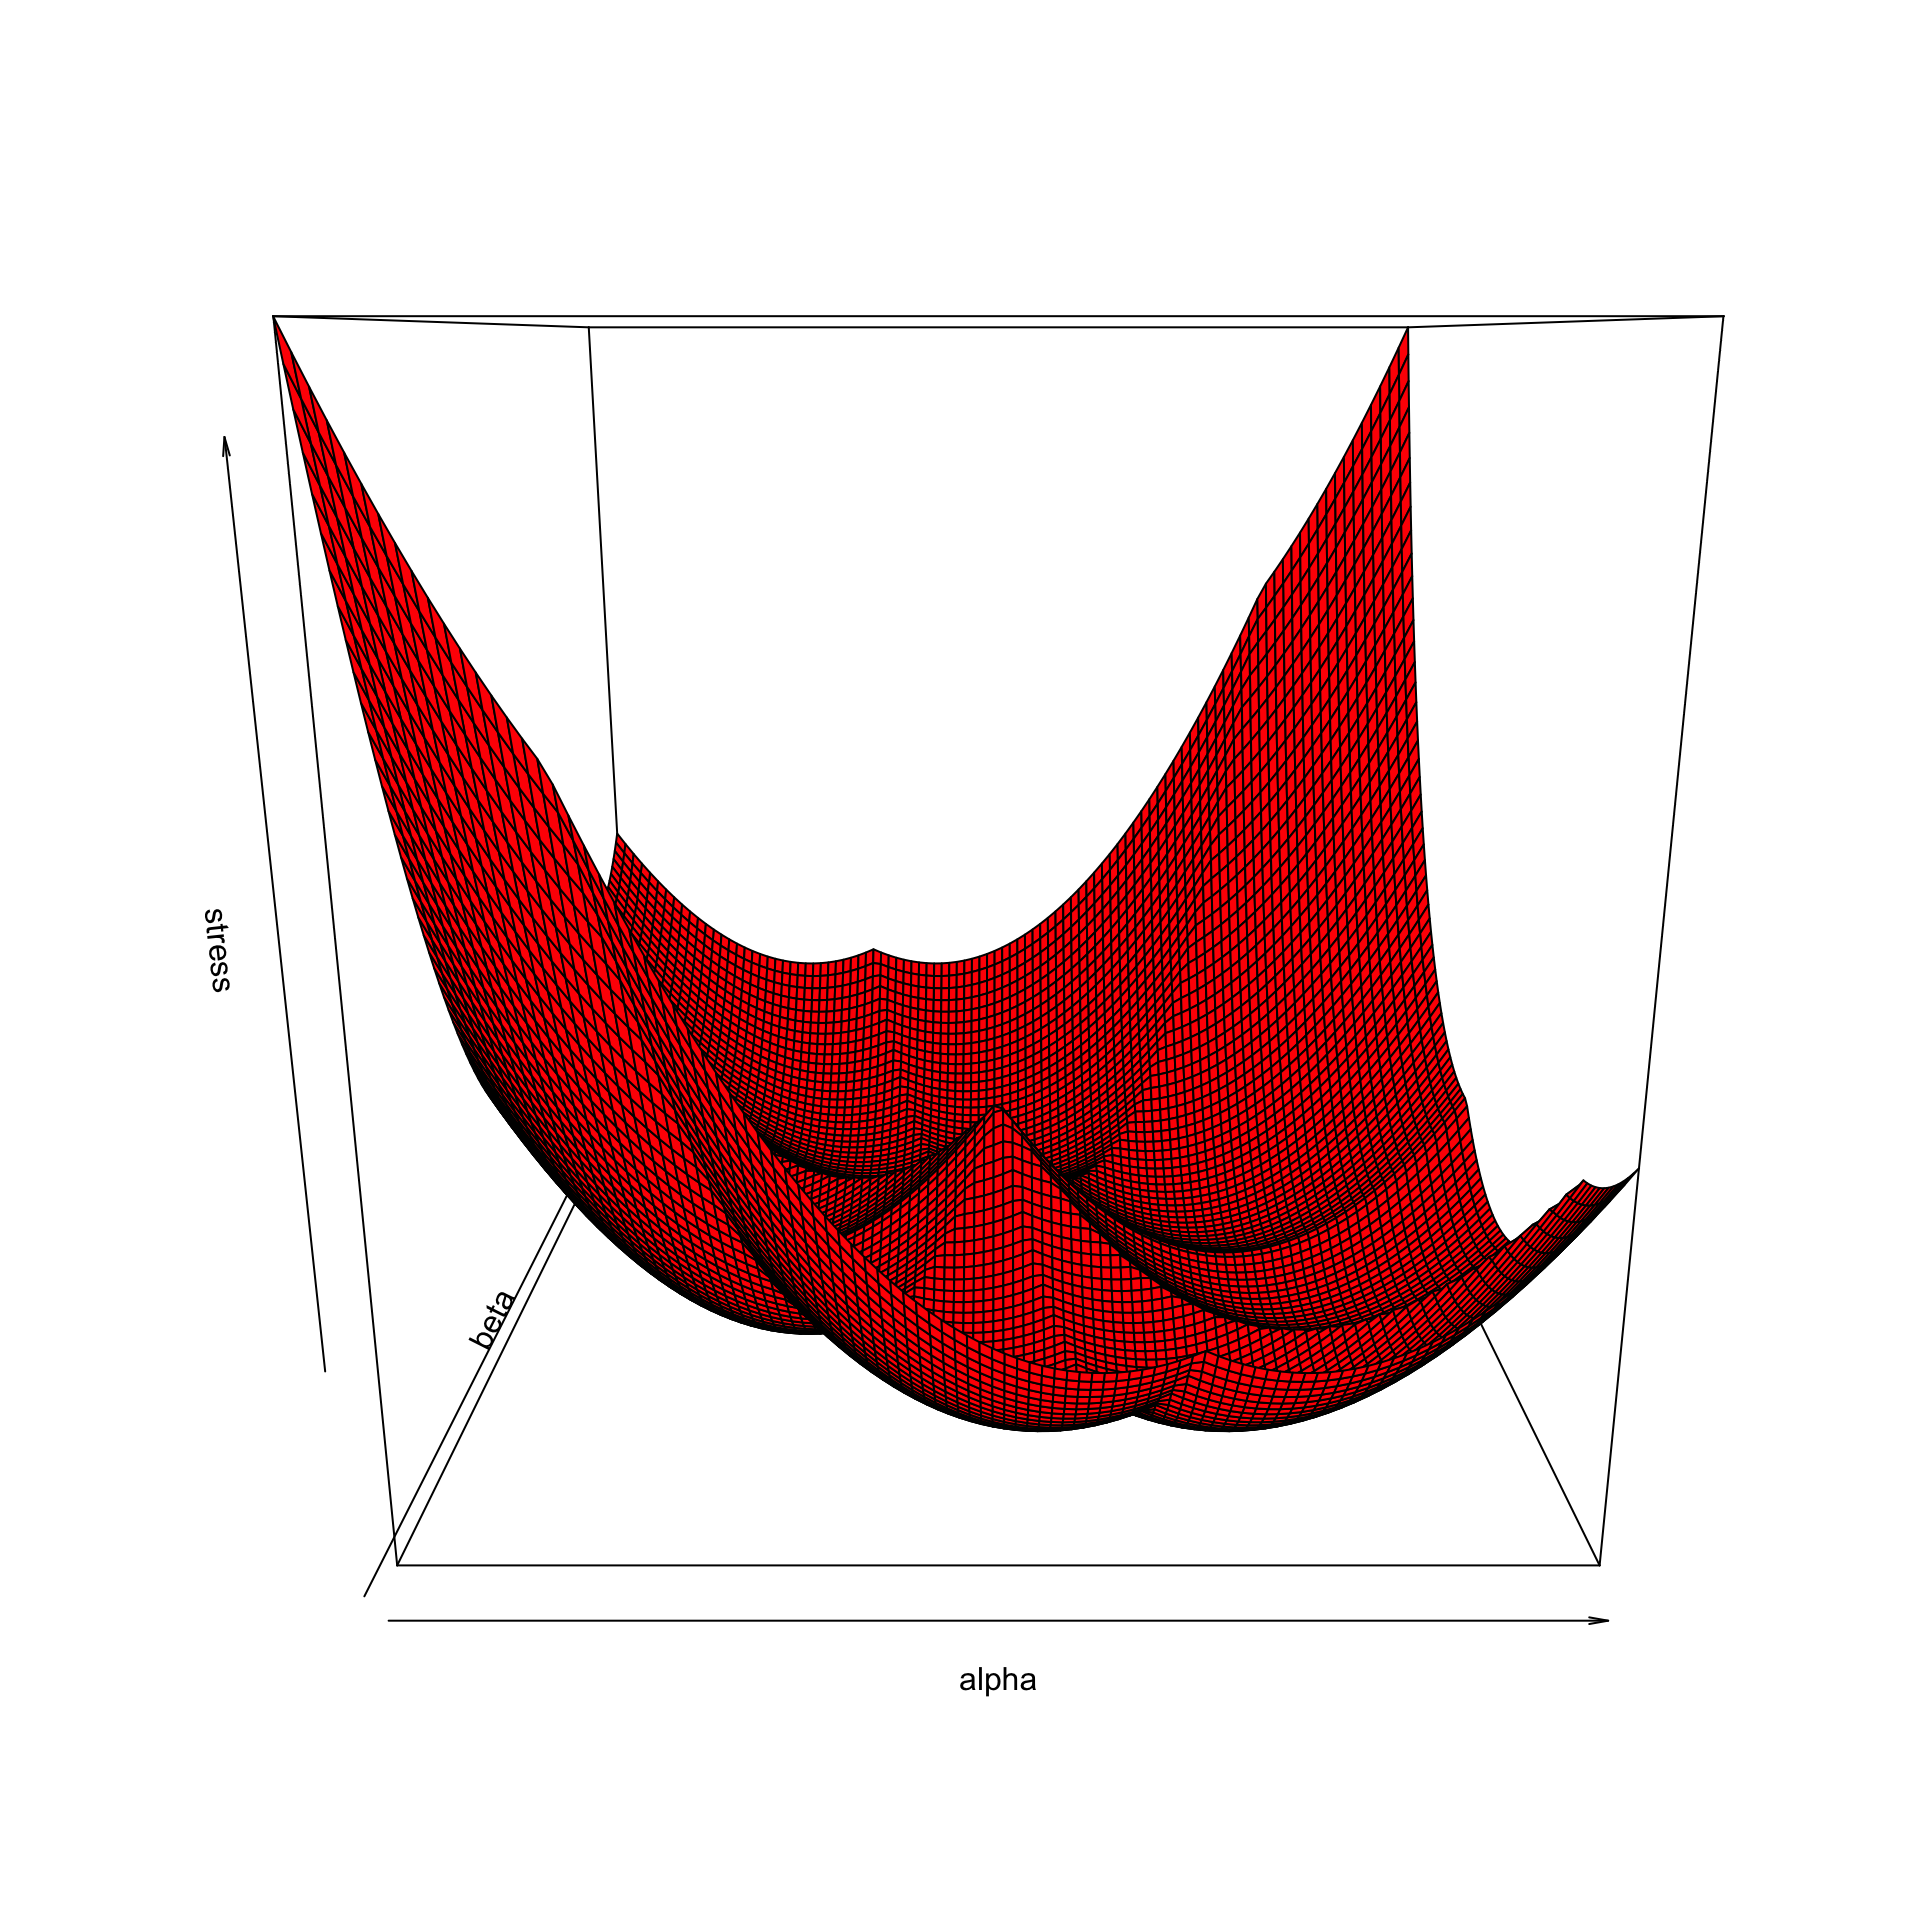
\includegraphics{unidimensional_files/figure-pdf/global_perspective2-1.pdf}
\end{center}

What do we see ? Definitely more ridges and valleys than in the
two-dimensional example of chapter @ref(propchapter). In the
one-dimensional case there is a ridge wherever two coordinates are
equal, and thus one or more distances are zero. It is clear that at the
bottom of each of the valleys there sits a local minimum.

\subsection{Contour}\label{contour}

A contour plot gives some additional details. In the plot we have drawn
the four lines through the origin where one or more distances are zero
(in red), and we have drawn the curve where \(\eta^2(x)=\rho(x)\) (in
blue). Thus all local minima are on the blue line. The intersections of
the red and the blue lines are the local minima of stress restricted to
the red line. In those points there are both directions of ascent (along
the red lines, in both directions) and of descent (into the adjoining
valleys, in all directions).

\begin{center}
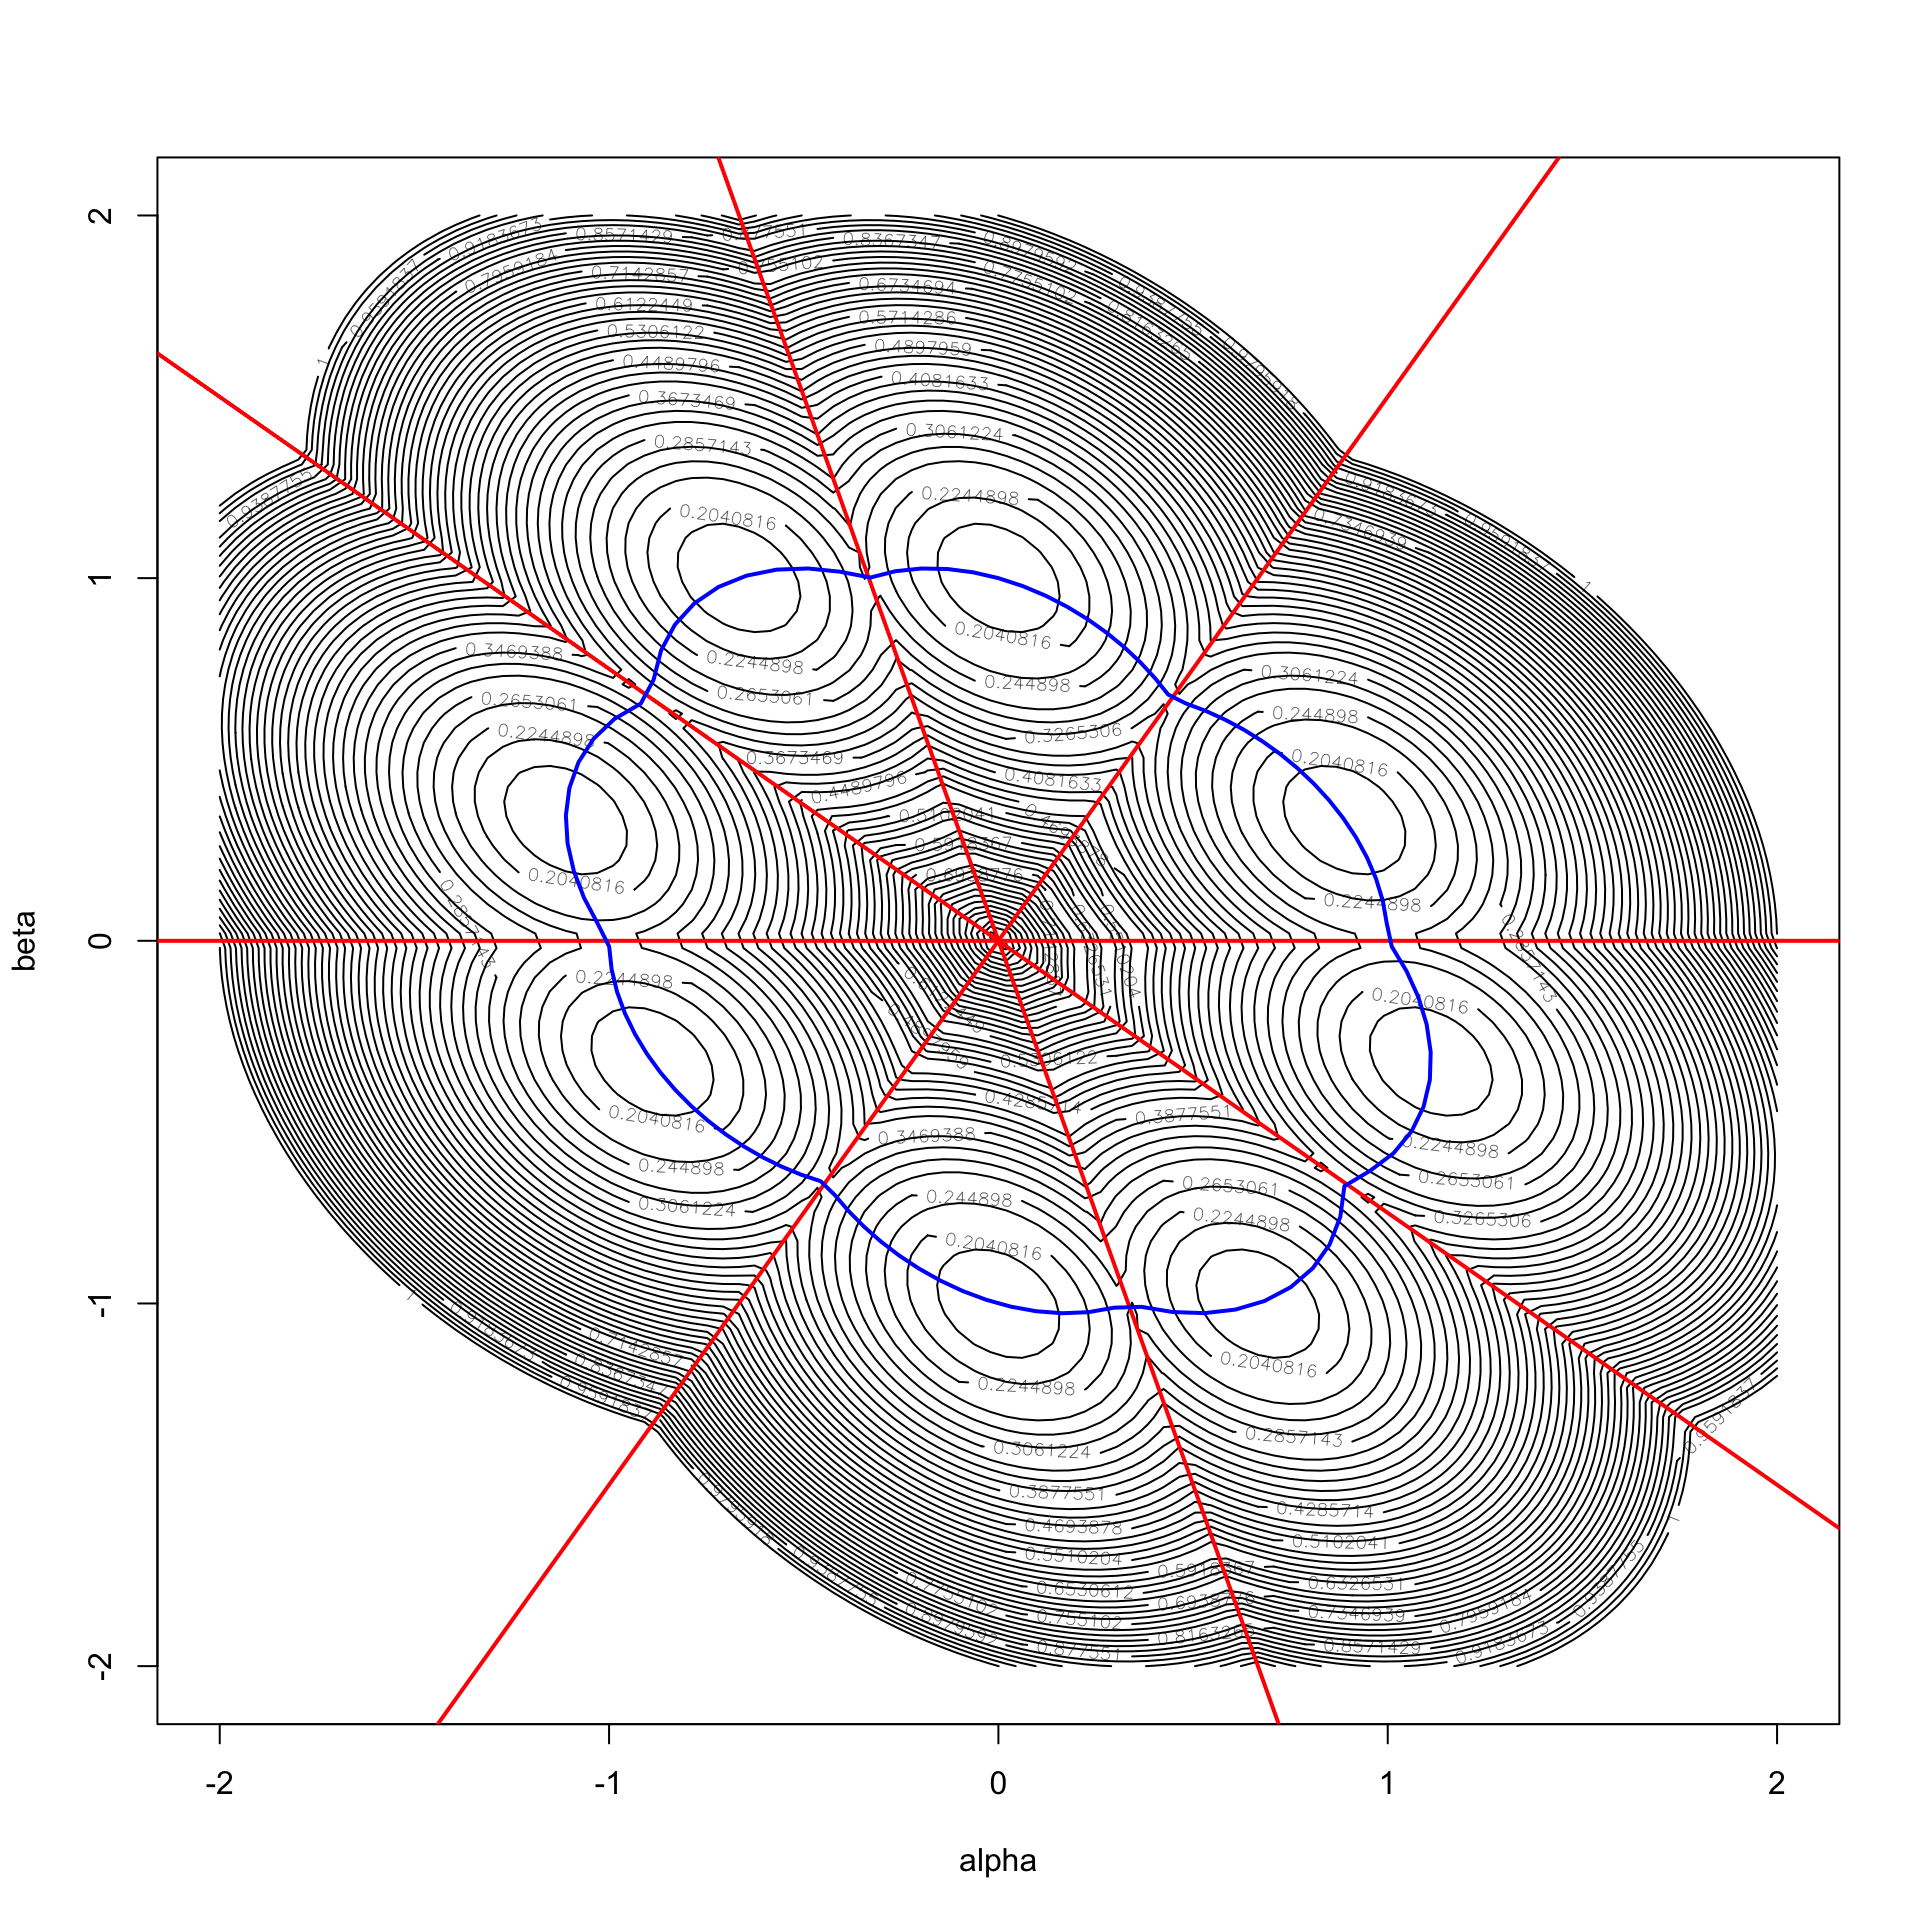
\includegraphics{unidimensional_files/figure-pdf/global_contour_one-1.pdf}
\end{center}

We see once more the importance of the local minimum result from De
Leeuw (\citeproc{ref-deleeuw_A_84f}{1984b}) that we discussed in section
@ref(proplocmin). The special relevbance of this result for UMDS was
already pointed out by Pliner (\citeproc{ref-pliner_96}{1996}). At a
local minimum all distances are positive, and thus local minima must be
in the interior of the eight cones defined by the four zero-distance
lines. There are no saddle points, and only a single local maximum at
the origin.

\section{Order Formulation}\label{order-formulation}

Define an \emph{isocone} as a closed convex cone of isotone vectors, and
\(\text{int}(K)\) as its interior. Thus

\begin{equation}
K:=\{x\in\mathbb{R}^n\mid x_{i_1}\leq\cdots\leq x_{i_n}\},
(\#eq:isoconc)
\end{equation}

and

\begin{equation}
\text{int}(K)=\{x\in\mathbb{R}^n\mid x_{i_1}<\cdots< x_{i_n}\}.
(\#eq:isoconi)
\end{equation}

where \((i_1,\cdots,i_n)\) is a permutation of \((1,\cdots,n)\). There
are \(n!\) such closed isocones, and their union is all of
\(\mathbb{R}^n\). Thus
\(\min_x\sigma(x)=\min_{K\in\mathcal{K}}\min_{x\in K}\sigma(x)=\,\)
where \(\mathcal{K}\) are the \(n!\) isocones.

For UMDS purposes the isocones are paired, because the negative of each
configuration has the same distances between the \(n\) points, and thus
the same stress. Thus each isocone and its negative cone are equivalent
for UMDS, and we only have to consider \((n!)/2\) distinct orders.

Let us consider the problem of minimizing \(\sigma\) over a fixed
\(K\in\mathcal{K}\). Now \[
\rho(x)=\mathop{\sum\sum}_{1\leq i<j\leq n}w_{ij}\delta_{ij}s_{ij}(x_i-x_j),
\] and \(s_{ij}=\text{sign}(x_i-x_j)\) is the sign matrix of \(x\).

\(S(x)\) is the \emph{sign matrix} of \(x\in\mathbb{R}^n\) if
\(s_{ij}(x)=\text{sign}(x_i-x_j)\) for all \(i\) and \(j\), i.e.

\begin{equation}
s_{ij}(x):=\begin{cases}+1&\text{ if }x_i>x_j,\\
-1&\text{ if }x_i<x_j,\\
\hfill 0&\text{ if }x_i=x_j.
\end{cases}
(\#eq:signdef)
\end{equation}

The set of all sign matrices is \(\mathcal{S}\).

Sign matrices are hollow and anti-symmetric. A sign matrix \(S\) is
\emph{strict} if its only zeroes are on the diagonal,
i.e.~\(S=S(P\iota)\) for some permutation matrix \(P\). The set of
strict sign matrices is \(\mathcal{S}_+\). Since there is a 1:1
correspondence between strict sign matrices and permutations, there are
\(n!\) strict sign matrices. The row sums and column sums of a strict
sign matrix are some permutation of the numbers \(n-2\iota+1\).

For all \(x\in\text{int}(K)\) the matrix \(S\) is the same strict sign
matrix. Now \[
\rho(x)=\frac12\sum_{i=1}^n\sum_{j=1}^nw_{ij}\delta_{ij}s_{ij}(x_i-x_j)=x't_K,
\] where \(t_K\) is the vector of row sums of the Hadamard product
\(W\times\Delta\times S\), or

\[
\{t_K\}_i:=\sum_{j=1}^nw_{ij}\delta_{ij}s_{ij}.
\] Again \(t_K\) only depends of \(K\), not on \(x\) as long as
\(x\in\text{int}(K)\).

Thus on \(K\)

\[
\sigma(x)=1-2x't_K+x'Vx=1+(x-V^{-1}t_K)'V(x-V^{-1}t_K)-t_K'V^{-1}t_K^{\ }.
\]

If there are no weights the \(t_K\) were first defined using isocones in
De Leeuw and Heiser (\citeproc{ref-deleeuw_heiser_C_77}{1977}). They
point out that minimizing \((x-V^{-1}t)'V(x-V^{-1}t)\) over \(x\in K\)
is a monotone regression problem (see @ref(mathmonreg)).

A crucial next step is in De Leeuw
(\citeproc{ref-deleeuw_C_05h}{2005b}), using the basic result in De
Leeuw (\citeproc{ref-deleeuw_A_84f}{1984b}). De Leeuw
(\citeproc{ref-deleeuw_C_05h}{2005b}) does use weights. We know if \(x\)
is a local minimum then it must be in the interior of the isocone. If
\(V^{-1}t_K\) is not in interior, then monotone regression will creates
ties, and thus \(x\) will not be in the interior either. In fact for
local minima of UMDS it is necessary and sufficient that \(V^{-1}t_K\)
is in the interior of \(K\). This result, without weights and in
somewhat different language, is also in Pliner
(\citeproc{ref-pliner_84}{1984}). Thus we can limit our search to those
isocones for which \(V^{-1}t_K\in\text{int}(K)\). For those isocones,
say the set \(\mathcal{K}^\circ\), the local minimum is at
\(x=V^{-1}t_K\).

Thus \[
\min_{K\in\mathcal{K}}\min_{x\in K}\sigma(x)=1 -\max_{K\in\mathcal{K}^\circ}\ t_K'V^{-1}t_K^{\ }.
\] There is also an early short but excellent paper by Defays
(\citeproc{ref-defays_78}{1978}), which derives basically the same
result in a non-geometrical way. Defays does not use weights, so in his
paper \(V^{-1}\) is \(n^{-1}I\).

In the two-dimensional subspace of the example some of the \(n!\) cones
are empty.

\section{Permutation Formulation}\label{permutation-formulation}

\section{Sign Matrix Formulation}\label{sign-matrix-formulation}

\begin{equation}
\rho(x)=\max_{S\in\mathcal{S}}\mathop{\sum\sum}_{1\leq i<j\leq n}w_{ij}\delta_{ij}s_{ij}(x_i-x_j),
(\#eq:rhosign)
\end{equation}

with the maximum attained for \(S=S(x)\). If we define

\begin{equation}
t_i(y):=\sum_{j=1}^n w_{ij}\delta_{ij}s_{ij}(y),
(\#eq:tdef)
\end{equation}

then

\begin{equation}
\sigma(x)=\min_y\{1+(x-V^{-1}t(y))'V(x-V^{-1}t(y))-t(y)'V^{-1}t(y)\}.
(\#eq:unipart)
\end{equation}

This implies

\begin{equation}
\min_x\sigma(x)= 1 - \max_y\ t(y)'V^{-1}t(y)
(\#eq:unidual)
\end{equation}

\section{Algorithms for UMDS}\label{unialgorithms}

\subsection{SMACOF}\label{unismacof}

\subsection{SMACOF (smoothed)}\label{unismoothed}

Now local minimum \(x_i\not= x_j\)

\[
\min_{x\in K}\sigma(x)=\mathop{\sum\sum}_{1\leq i<j\leq n}w_{ij}(\delta_{ij}-s_{ij}(x))(x_i-x_j))^2
\]

Each isocone has a sign matrix (hollow, antisymmetric)

\[
s_{ij}(x)=\begin{cases}+1&\text{ if }x_i>x_j,\\
-1&\text{ if }x_i<x_j,\\
\hfill 0&\text{ if }x_i=x_j.
\end{cases}
\] \[
\rho(x)=\sum_{i=1}^n\sum_{j=1}^nw_{ij}\delta_{ij}s_{ij}(x)(x_i-x_j)\geq
\sum_{i=1}^n\sum_{j=1}^nw_{ij}\delta_{ij}s_{ij}(y)(x_i-x_j)=
2\sum_{i=1}^n x_i\sum_{j=1}^n w_{ij}\delta_{ij}s_{ij}(y)
\]

Now

\begin{equation}
\rho(x)=\sum_{i=1}^n\sum_{j=1}^nw_{ij}\delta_{ij}s_{ij}(x)(x_i-x_j),
\end{equation}

and for all \(y\in\mathbb{R}^n\)

\begin{equation}
\rho(x)\geq
\sum_{i=1}^n\sum_{j=1}^nw_{ij}\delta_{ij}s_{ij}(y)(x_i-x_j)=
2\sum_{i=1}^n x_i\sum_{j=1}^n w_{ij}\delta_{ij}s_{ij}(y).
\end{equation}

Stress is the maximum of a finite number of quadratics.

\subsection{Branch-and-Bound}\label{unibranchbound}

\subsection{Dynamic Programming}\label{unidynamic}

\subsection{Simulated Annealing}\label{uniannealing}

\subsection{Penalty Methods}\label{unipenalty}

\bookmarksetup{startatroot}

\chapter{Full-dimensional Scaling}\label{fullchapter}

\section{Convexity}\label{fullconvex}

\section{Optimality}\label{fulloptimal}

\section{Iteration}\label{fulliteration}

\section{Cross Product Space}\label{fullcpspace}

So far we have formulated the MDS problem in \emph{configuration space}.
Stress is a function of \(X\), the \(n\times p\) configuration matrix.
We now consider an alternative formulation, where stress is a function
of a positive semi-definite \(C\) or order \(n\). The relevant
definitions are \begin{equation}
\sigma(C):=1-2\rho(C)+\eta(C),
\end{equation} where \begin{align*}
\rho(C)&:=\mathbf{tr}\ B(C)C,\\
\eta(C)&:=\mathbf{tr}\ VC,
\end{align*} with \begin{equation*}
B(C):=\mathop{\sum\sum}_{1\leq i<j\leq n} \begin{cases}w_{ij}\frac{\delta_{ij}}{d_{ij}(C)}A_{ij}&\text{ if }d_{ij}(C)>0,\\
0&\text{ if }d_{ij}(C)=0.\end{cases}
\end{equation*} and \(d_{ij}^2(C):=\mathbf{tr}\ A_{ij}C\).

We call the space of all positive semi-definite \(n\times n\) matrices
\emph{cross product space}. The problem of minimizing \(\sigma\) over
\(n\times p\)-dimensional configuration space is equivalent to the
problem of minimizing \(\sigma\) over the set of matrices \(C\) in
\(n\times n\)-dimensional cross product space that have rank less than
or equal to \(p\). The corresponding solutions are related by the simple
relationship \(C=XX'\).

\begin{Shaded}
\begin{Highlighting}[]
\NormalTok{Stress is convex on cross product space.}
\end{Highlighting}
\end{Shaded}

\begin{proof}
First, \(\eta\) is linear in \(C\). Second, \[
\rho(C)=\mathop{\sum\sum}_{1\leq i<j\leq n} w_{ij}\delta_{ij}\sqrt{\mathbf{tr}\ A_{ij}C}.
\] This is the weighted sum of square roots of non-negative functions
that are linear in \(C\), and it is consequently concave. Thus
\(\sigma\) is convex.
\end{proof}

Unfortunately the subset of cross product space of all matrices with
rank less than or equal to \(p\) is far from simple (see
(\citeproc{ref-datorro_15}{\textbf{datorro\_15?}})), so computational
approaches to MDS prefer to work in configuration space.

\section{Full-dimensional Scaling}\label{full-dimensional-scaling}

Cross product space, the set of all positive semi-definite matrices, is
a closed convex cone \(\mathcal{K}\) in the linear space of all
\(n\times n\) symmetric matrices. This has an interesting consequence.

\begin{Shaded}
\begin{Highlighting}[]
\NormalTok{Full{-}dimensional scaling, i.e. minimizing $\textbackslash{}sigma$ over $\textbackslash{}mathcal\{K\}$, is a convex programming problem. Thus in FDS all local minima are global. If $w\_\{ij\}\textbackslash{}delta\_\{ij\}\textgreater{}0$ for all $i,j$ then the minimum is unique.}
\end{Highlighting}
\end{Shaded}

This result has been around since about 1985. De Leeuw
(\citeproc{ref-deleeuw_R_93c}{1993}) gives a proof, but the report it
appeared in remained unpublished. A published proof is in {``{Inverse
Multidimensional Scaling}''}
(\citeproc{ref-deleeuw_groenen_A_97}{2007}). Another treatment of FDS,
with a somewhat different emphasis, is in De Leeuw
(\citeproc{ref-deleeuw_U_14b}{2014a}).

Now, by a familiar theorem (Theorem 31.4 in Rockafellar
(\citeproc{ref-rockafellar_70}{1970})), a matrix \(C\) minimizes
\(\sigma\) over \(\mathcal{K}\) if and only if \begin{align}
C&\in\mathcal{K},\\
V-B(C)&\in\mathcal{K},\\
\mathbf{tr}\ C(V-B(C))&=0.
\end{align} We give a computational proof of this result for FDS that
actually yields a bit more.

\begin{Shaded}
\begin{Highlighting}[]
\NormalTok{For $\textbackslash{}Delta\textbackslash{}in\textbackslash{}mathcal\{K\}$ we have}
\NormalTok{\textbackslash{}begin\{equation\}}
\NormalTok{\textbackslash{}sigma(C+\textbackslash{}epsilon\textbackslash{}Delta)=\textbackslash{}sigma(C){-}2\textbackslash{}epsilon\^{}\{\textbackslash{}frac12\}\textbackslash{}sum\_\{\textbackslash{}mathbf\{tr\}\textbackslash{} A\_iC = 0\}w\_i\textbackslash{}delta\_i\textbackslash{}sqrt\{\textbackslash{}mathbf\{tr\}\textbackslash{} A\_i\textbackslash{}Delta\}+\textbackslash{}epsilon\textbackslash{} \textbackslash{}mathbf\{tr\}\textbackslash{} (V{-}B(C))\textbackslash{}Delta}
\NormalTok{+o(\textbackslash{}epsilon).\textbackslash{}label\{E:expand\}}
\NormalTok{\textbackslash{}end\{equation\}}
\end{Highlighting}
\end{Shaded}

\begin{proof}
Simple expansion.
\end{proof}

\begin{center}\rule{0.5\linewidth}{0.5pt}\end{center}

\begin{Shaded}
\begin{Highlighting}[]
\NormalTok{Suppose $C$ is a solution to the problem of minimizing $\textbackslash{}sigma$ over $\textbackslash{}mathcal\{K\}$. Then}

\NormalTok{* $\textbackslash{}mathbf\{tr\}\textbackslash{} A\_\{ij\}C \textgreater{} 0$ for all $i,j$ for which $w\_\{ij\}\textbackslash{}delta\_\{ij\}\textgreater{}0$.}
\NormalTok{* $V{-}B(C)$ is positive semi{-}definite.}
\NormalTok{* $\textbackslash{}mathbf\{tr\}\textbackslash{} C(V{-}B(C))=0$.}
\NormalTok{* If $C$ is positive definite then $V=B(C)$ and $\textbackslash{}sigma(C)=0$.}
\end{Highlighting}
\end{Shaded}

\begin{center}\rule{0.5\linewidth}{0.5pt}\end{center}

\begin{proof}
The \(\epsilon^\frac12\) term in \(\eqref{E:expand}\) needs to vanish at
a local minimum. This proves the first part. It follows that at a local
minimum

\begin{equation*}
\sigma(C+\epsilon\Delta)=\sigma(C)+
\epsilon\ \mathbf{tr}\ (V-B(C))\Delta+o(\epsilon).
\end{equation*}

If \(V-B(C)\) is not positive semi-definite, then there is a
\(\Delta\in\mathcal{K}\) such that \(\mathbf{tr}\ (V-B(C))\Delta < 0\).
Thus \(C\) cannot be the minimum, which proves the second part. If we
choose \(\Delta=C\) we find

\begin{equation*}
\sigma((1+\epsilon)C)=\sigma(C)+
\epsilon\ \mathbf{tr}\ (V-B(C))C+o(\epsilon).
\end{equation*}

and choosing \(\epsilon\) small and negative shows we must have
\(\mathbf{tr}\ (V-B(C))C=0\) for \(C\) to be a minimum. This proves the
third part. Finally, if \(\sigma\) has a minimum at \(C\), and \(C\) is
positive definite, then from parts 2 and 3 we have \(V=B(C)\). Comparing
off-diagonal elements shows \(\Delta=D(C)\), and thus \(\sigma(C)=0\).
\end{proof}

If \(C\) is the solution of the FDS problem, then \(\mathbf{rank}(C)\)
defines the \emph{Gower rank} of the dissimilarities. The number of
positive eigenvalues of the negative of the doubly-centered matrix of
squared dissimilarities, the matrix factored in classical MDS, defines
the \emph{Torgerson rank} of the dissimilarities. The \emph{Gower
conjecture} is that the Gower rank is less than or equal to the
Torgerson rank. No proof and no counter examples have been found.

We compute the FDS solution using the smacof algorithm \begin{equation}
X^{(k+1)}=V^+B(X^{(k)})
\end{equation} in the space of all \(n\times n\) configurations, using
the identity matrix as a default starting point. Since we work in
configuration space, not in crossproduct space, this does not guarantee
convergence to the unique FDS solution, but after convergence we can
easily check the necessary and sufficient conditions of theorem
@ref(thm:rockafellar).

As a small example, consider four points with all dissimilarities equal
to one, except \(\delta_{14}\) which is equal to three. Clearly the
triangle inequality is violated, and thus there certainly is no perfect
fit mapping into Euclidean space.

The FDS solution turns out to have rank two, thus the Gower rank is two.
The singular values of the FDS solution are

\begin{verbatim}
[1] 0.4508464709 0.2125310645 0.0000001303
\end{verbatim}

Gower rank two also follows from the eigenvalues of the matrix \(B(C)\),
which are

\begin{verbatim}
[1] 1.0000000000 1.0000000000 0.9205543464
\end{verbatim}

\section{Ekman example}\label{ekman-example-1}

The Ekman (\citeproc{ref-ekman_54}{1954}) color data give similarities
between 14 colors.

\begin{verbatim}
     434  445  465  472  490  504  537  555  584  600  610  628  651
445 0.86                                                            
465 0.42 0.50                                                       
472 0.42 0.44 0.81                                                  
490 0.18 0.22 0.47 0.54                                             
504 0.06 0.09 0.17 0.25 0.61                                        
537 0.07 0.07 0.10 0.10 0.31 0.62                                   
555 0.04 0.07 0.08 0.09 0.26 0.45 0.73                              
584 0.02 0.02 0.02 0.02 0.07 0.14 0.22 0.33                         
600 0.07 0.04 0.01 0.01 0.02 0.08 0.14 0.19 0.58                    
610 0.09 0.07 0.02 0.00 0.02 0.02 0.05 0.04 0.37 0.74               
628 0.12 0.11 0.01 0.01 0.01 0.02 0.02 0.03 0.27 0.50 0.76          
651 0.13 0.13 0.05 0.02 0.02 0.02 0.02 0.02 0.20 0.41 0.62 0.85     
674 0.16 0.14 0.03 0.04 0.00 0.01 0.00 0.02 0.23 0.28 0.55 0.68 0.76
\end{verbatim}

We use three different transformations of the similarities to
dissimilarities. The first is \(1-x\), the second \((1-x)^3\) and the
third \(\sqrt[3]{1-x}\). We need the following iterations to find the
FDS solution (up to a change in loss of 1e-15).

\begin{verbatim}
power =  1.00  itel =    6936  stress =  0.0000875293 
power =  3.00  itel =     171  stress =  0.0110248119 
power =  0.33  itel =     423  stress =  0.0000000000 
\end{verbatim}

For the same three solutions we compute singular values of the
thirteen-dimensional FDS solution.

\begin{verbatim}
 [1] 0.1797609824 0.1454675297 0.0843865491 0.0777136109 0.0486123551
 [6] 0.0393576522 0.0236290817 0.0162344515 0.0072756171 0.0000031164
[11] 0.0000000009 0.0000000000 0.0000000000

 [1] 0.2159661347 0.1549184093 0.0000000727 0.0000000041 0.0000000000
 [6] 0.0000000000 0.0000000000 0.0000000000 0.0000000000 0.0000000000
[11] 0.0000000000 0.0000000000 0.0000000000

 [1] 0.1336126813 0.1139019875 0.0880453752 0.0851609618 0.0710424935
 [6] 0.0664988952 0.0561005006 0.0535112029 0.0492295395 0.0479964575
[11] 0.0468628701 0.0410193579 0.0388896490
\end{verbatim}

Thus the Gower ranks of the transformed dissimilarities are,
repectively, nine (or ten), two, and thirteen. Note that for the second
set of dissimilarities, with Gower rank two, the first two principal
components of the thirteen-dimensional solution are the global minimizer
in two dimensions. To illustrate the Gower rank in yet another way we
give the thirteen non-zero eigenvalues of \(V^+B(X)\), so that the Gower
rank is the number of eigenvalues equal to one. All three solutions
satisfy the necessary and sufficient conditions for a global FDS
solution.

\begin{verbatim}
 [1] 1.0000000432 1.0000000222 1.0000000012 1.0000000005 1.0000000002
 [6] 1.0000000001 1.0000000000 1.0000000000 0.9999993553 0.9989115116
[11] 0.9976821885 0.9942484083 0.9825147154

 [1] 1.0000000000 1.0000000000 0.9234970864 0.9079012130 0.8629365849
 [6] 0.8526920031 0.8298036209 0.8145561677 0.7932385763 0.7916517225
[11] 0.7864426781 0.7476794757 0.7282682474

 [1] 1.0000000820 1.0000000241 1.0000000047 1.0000000009 1.0000000004
 [6] 1.0000000003 1.0000000001 1.0000000001 1.0000000001 1.0000000000
[11] 0.9999999999 0.9999999689 0.9999999005
\end{verbatim}

We also plot the first two principal components of the
thirteen-dimensional FDS solution. Not surprisingly, they look most
circular and regular for the solution with power three, because this
actually is the global minimum over two-dimensional solutions. The other
configurations still have quite a lot of variation in the remaining
dimensions.

\begin{figure}[H]

{\centering 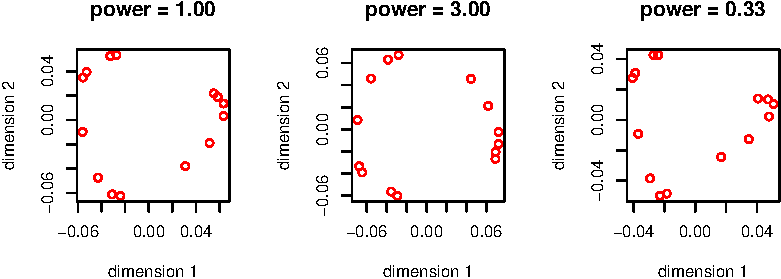
\includegraphics{full_files/figure-pdf/ekmanconfs-1.pdf}

}

\caption{Ekman data, configurations for three powers}

\end{figure}%

Figure @ref\{fig:ekmantrans\} illustrates that the FDS solution with
power 3 is quite different from power 1 and power one \(1/3\) Basically
the transformations with lower powers result in dissimilarity measures
that are very similar to Euclidean distances in a high-dimensional
configuration, while power equal to 3 makes the dissimilarties less
Euclidean. This follows from metric transform theory, where concave
increasing transforms of finite metric spaces tend to be Euclidean. In
particular the square root transformation of a finite metric space has
the Euclidean four-point property, and there is a \(c>0\) such that the
metric transform \(f(t)=ct/(1+ct)\) makes a finite metric space
Euclidean (Maehara (\citeproc{ref-maehara_86}{1986})).

\begin{figure}[H]

{\centering \includegraphics{full_files/figure-pdf/ekmantrans-1.pdf}

}

\caption{Ekman data, fit plots for three powers}

\end{figure}%

\bookmarksetup{startatroot}

\chapter{Unfolding}\label{chunfolding}

In unfolding the objects are partitioned into two sets of, say, \(n\)
and \(m\) objects and only the \(nm\) between-set dissimilarities are
observed. The within-set weights are zero. Thus we minimize
\begin{equation}
\sigma(X,Y)=\sum_{i=1}^n\sum_{j=1}^m w_{ij}(\delta_{ij}-d(x_i,y_j))^2
(\#eq:unfstress)
\end{equation} over \(X\in\mathbb{R}^{n\times p}\) and
\(Y\in\mathbb{R}^{m\times p}\).

\(\frac12\{(n+m)(n+m-1)-2nm\}\) are missing

note that we can have \(d_{ij}(X)=0\) at a local minimum.

\section{Algebra}\label{algebra-1}

The missing data in unfolding complicate the MDS problem, in the same
way as the singular value decomposition of a rectangular matrix is more
complicated than the eigen decomposition of a symmetric matrix.

The problem we want to solve in this section is recovering \(X\) and
\(Y\) (up to a translation and rotation) from \(D(X,Y)\).

The first matrix algebra results in metric unfolding were due to Ross
and Cliff (\citeproc{ref-ross_cliff_64}{1964}). An actual algorithm for
the ``ignore-errors'' case was proposed by Schönemann
(\citeproc{ref-schoenemann_70}{1970}). Schönemann's technique was
studied in more detail by Gold (\citeproc{ref-gold_73}{1973}) and Heiser
and De Leeuw (\citeproc{ref-heiser_deleeuw_A_79}{1979}).

This sectiom discusses a slightly modified version of Schönemann
(\citeproc{ref-schoenemann_70}{1970}).

First, we compute the Torgerson transform
\(E(X,Y)=-\frac12 JD^{(2)}(X,Y)J\) It was observed for the first time by
Ross and Cliff (\citeproc{ref-ross_cliff_64}{1964}) that
\(E(X,Y)=JXY'J\).

Assume that \(E(X,Y)=JXY'J\) is a full-rank decomposition, and that the
rank of \(E(X,Y)\) is \(r\). Note that there are cases in which the rank
of \(JX\) or \(JY\) is strictly smaller than the rank of \(X\) or \(Y\).
If \(X\), for example, has columns \(x\) and \(e-x\), with \(x\) and
\(e\) linearly independent, then its rank is two, while \(JX\) with
columns \(Jx\) and \(-Jx\) has rank one.

Suppose \(E(X,Y)=GH'\) is another full-rank decomposition. Then there
exist vectors \(u\) and \(v\) with \(r\) elements and a non-singular
\(T\) of order \(r\) such that \begin{align}
\begin{split}
X&=GT+eu',\\
Y&=HT^{-t}+ev'.
\end{split}
(\#eq:unfundet)
\end{align} We can assume without loss of generality that the centroid
of the \(X\) configuration is in the origin, so that \(JX=X\), and
\(u=0\) in the first equation of @ref(eq:unfundet).

We use the QR decomposition to compute the rank \(r\) of \(E(X,Y)\), and
the factors \(G\) and \(H\).

We now use @ref(eq:unfundet) to show that \(F=D^{(2)}(X,Y)+2GH'\) is of
the form \(F=\gamma+\alpha e'+e\beta'\), with \(\gamma=v'v\) and
\(M=TT'\).

\begin{align}
\begin{split}
\alpha_i&=g_i'Mg_i-2g_i'Tv,\\
\beta_j&=h_j'M^{-1}h_j+2h_j'T^{-t}v.
\end{split}
(\#eq:unfadditive)
\end{align}

It follows that \(JF=J\alpha e'\) and \(FJ=e\beta' J\). Thus \(J\alpha\)
is any column of \(JF\) and \(J\beta\) is any row of \(FJ\).

Consider the first equation of @ref(eq:unfadditive). For the time being,
we ignore the second one. Suppose \(M_k\) is a basis for the space of
real symmetric matrices of order \(p\) with the \(\frac12 p(p+1)\)
elements \(e_se_t'+e_te_s'\) for \(s\not= t\) and \(e_se_s'\) for the
diagonal. Define \(q_{ik}:=g_i'M_kg_i\). Then

\begin{equation}
J\alpha=J\begin{bmatrix}Q&-2G\end{bmatrix}\begin{bmatrix}\mu\\Tv\end{bmatrix},
(\#eq:unflinear)
\end{equation}

with \(\mu\) the coordinates of \(M\) for the basis \(M_k\).

Equations @ref(eq:unflinear) are \(n\) linear equations in the
\(\frac12 p(p+1)+p=\frac12 p(p+3)\) unknowns \(\mu\) and \(Tv\). Assume
they have a unique solution. Then \(M=\sum\mu_kM_k\) is PSD, and can be
eigen-decomposed as \(M=K\Lambda^2 K'\). Set \(T=K\Lambda\)

\begin{Shaded}
\begin{Highlighting}[]
\FunctionTok{set.seed}\NormalTok{(}\DecValTok{12345}\NormalTok{)}
\NormalTok{x }\OtherTok{\textless{}{-}} \FunctionTok{matrix}\NormalTok{ (}\FunctionTok{rnorm}\NormalTok{(}\DecValTok{16}\NormalTok{), }\DecValTok{8}\NormalTok{, }\DecValTok{2}\NormalTok{)}
\NormalTok{x }\OtherTok{\textless{}{-}} \FunctionTok{apply}\NormalTok{ (x, }\DecValTok{2}\NormalTok{, }\ControlFlowTok{function}\NormalTok{ (x) x }\SpecialCharTok{{-}} \FunctionTok{mean}\NormalTok{ (x))}
\NormalTok{y }\OtherTok{\textless{}{-}} \FunctionTok{matrix}\NormalTok{ (}\FunctionTok{rnorm}\NormalTok{(}\DecValTok{10}\NormalTok{), }\DecValTok{5}\NormalTok{, }\DecValTok{2}\NormalTok{)}
\NormalTok{a }\OtherTok{\textless{}{-}} \FunctionTok{rowSums}\NormalTok{ (x }\SpecialCharTok{\^{}} \DecValTok{2}\NormalTok{)}
\NormalTok{b }\OtherTok{\textless{}{-}} \FunctionTok{rowSums}\NormalTok{ (y }\SpecialCharTok{\^{}} \DecValTok{2}\NormalTok{)}
\NormalTok{d }\OtherTok{\textless{}{-}} \FunctionTok{sqrt}\NormalTok{ (}\FunctionTok{outer}\NormalTok{(a, b, }\StringTok{"+"}\NormalTok{) }\SpecialCharTok{{-}} \DecValTok{2} \SpecialCharTok{*} \FunctionTok{tcrossprod}\NormalTok{ (x, y))}
\end{Highlighting}
\end{Shaded}

\subsection{One-dimensional}\label{one-dimensional}

The one-dimensional case is of special interest, because it allows us to
construct an single joint metric scale for row objects and column
objects from metric dissimilarities. We have to find a solution to
\(\delta_{ij}=|x_i-y_j|\), without making assumptions about the order of
the projections on the dimension. Compute any solution for \(Jg\) and
\(Jh\) from \(\tau(\Delta^{(2)})=Jgh'J\). For data with errors we would
probably use the SVD. Assume without loss of generality that \(Jg=g\).
Then the general solution is \(x=\tau g\) and \(y=\tau^{-1}h+\nu e\) for
some real \(\tau\) and \(\nu\).

Now

\begin{equation}
\Delta^2=\tau^2 g^{(2)}e'+\tau^{-2}e(h_j')^{(2)}+\nu^2E-2gh'-2\tau\nu g_ie'
(\#eq:schone)
\end{equation}

are \(nm\) equations in the two unknowns \((\tau,\nu)\). They can be
solved by many methods, but we go the Schönemann way. Column-centering
gives

\begin{equation}
J(\Delta^{(2)}+2g_jh_j)=\tau^2 Jg^{(2)}-2\tau\nu g,
(\#eq:schonecol)
\end{equation}

while row-centering gives

\begin{equation}
(\Delta^{(2)}+2g_jh_j)J=\tau^{-2}e(h^{(2)})'J.
(\#eq:schonerow)
\end{equation}

\section{Classical Unfolding}\label{classical-unfolding}

Multidimensional unfolding as a data analysis technique was introduced
by Coombs (\citeproc{ref-coombs_64}{1964}).

bennett-hays hays-bennett bennett

SMACOF - Heiser and De Leeuw (\citeproc{ref-heiser_deleeuw_A_79}{1979})

Form of V

What happens to nonzero theorem ? within-set distances can be zero

\(\Delta=\begin{bmatrix}1&2&3\\1&2&3\end{bmatrix}\)

\(x_1=x_2=0\) \(y_1=1,y_2=2,y_3=3\)

\section{Nonmetric Unfolding}\label{nonmetric-unfolding}

row-conditional busing van deun deleeuw\_R\_06a

Stress3 -- Roskam

\subsection{Degenerate Solutions}\label{unfdegenerate}

What are they

\subsubsection{Which Stress}\label{which-stress}

\[
\sigma(X)=\sum_{i=1}^n\sum_{j=1}^n w_{ij}(\delta_{ij}-d_{ij}(X))^2
\] Weak order, plus normalization. Two-point solution.

\subsubsection{l'Hôpital's Rule}\label{hopital}

We all know that \(0/0\) is not defined and should be avoided at all
cost. But then again we have \[
\lim_{x\rightarrow 0}\frac{\sin(x)}{x}=\cos(0)=1,
\] and in fact \(\sup_x \frac{sin(x)}{x}=1\). Or, for that matter, if
\(f\) is differentiable at \(x\) then

\[
\lim_{\epsilon\rightarrow 0}\frac{f(x+\epsilon)-f(x)}{\epsilon}=f'(x)
\] If \(f:\mathbb{R}\Rightarrow\mathbb{R}\) and
\(g:\mathbb{R}\Rightarrow\mathbb{R}\) are two functions

\begin{itemize}
\tightlist
\item
  differentiable in an interval \(\mathcal{I}\), except possibly at
  \(c\in\mathcal{I}\),
\item
  \(g'(x)\not=0\) for all \(x\in\mathcal{I}\),
\item
  \(\lim_{x\rightarrow c}f(x)=\lim_{x\rightarrow c}g(x)=0\) or
  \(\lim_{x\rightarrow c}f(x)=\lim_{x\rightarrow c}g(x)=\pm\infty\),
  then \[
  \lim_{x\rightarrow c}\frac{f(x)}{g(x)}=\lim_{x\rightarrow c}\frac{f'(x)}{g'(x)}
  \]
\end{itemize}

We use l'Hôpital's rule in chapter @ref(chunfolding), section
@ref(unfdegenerate) on degeneracies in nonmetric unfolding. We have not
explored the multivariate versions of l'Hôpitals rule, discussed for
example by Lawlor (\citeproc{ref-lawlor_20}{2020}).

Illustration.

\(\delta_{12}>\delta_{13}=\delta_{23}\).

\(d_{12}(X_\epsilon)=1\)

\(d_{13}(X_\epsilon)=d_{23}(X_\epsilon)=1+\frac12\epsilon\).

Then

\(\lim_{\epsilon\rightarrow 0}D(X_\epsilon)=\Delta\).

euclidean for \(\epsilon\geq-1\)

\subsubsection{Penalizing}\label{penalizing}

\subsubsection{Restricting Regression}\label{restricting-regression}

Busing

Van Deun

\bookmarksetup{startatroot}

\chapter{Constrained Multidimensional Scaling}\label{cmds}

As we have seen in section @ref(introgeneralize) Constrained
Multidimensional Scaling or CMDS is defined as the generalization of
basic MDS in which we want to solve \[
\min_{X\in\Omega}\ \mathop{\sum\sum}_{1\leq i<j\leq n}w_{ij}(\delta_{ij}-d_{ij}(X))^2,
\] where \(\Omega\) is a subset of \(\mathbb{R}^{n\times p}\). Of course
there are also versions of CMDS in which the dissimilarities are
nonmetric and must be quantified or transformed accordingly. But in this
chapter we concentrate on the ways in which we constrain the
configuration and on the ways to incorporate this into the smacof
framework.

Constraints on \(X\) can be defined in many different ways. They can be
in \emph{parametric form}, using a map
\(F:\Theta\Rightarrow\mathbb{R}^{n\times p}\). Thus the constraints are
\(X=F(\theta)\) and \(\theta\) varies in some subset \(\Theta\) of real
parameter space. Alternatively we can have constraints in \emph{dual
form}, i.e, have a maps~\(F\) on \(\mathbb{R}^{n\times p}\) and define
\(\Omega\) by \(F(X)=0\) (or \(F_1(X)=0\) and \(F_2(X)\geq 0\)). If
\(F\) is smooth both parametric and dual forms define manifolds in
\(\mathbb{R}^{n\times p}\), and often constraints can be equivalently
expressed in both forms. Requiring the points in the configuration to be
on the unit circle, for example, has the parametric form
\(x_i=(\sin\theta_i,\cos\theta_i)\) and the dual form \(\|x_i\|^2=1\).

Bentler-Weeks

\[
\mathop{\sum\sum}_{1\leq i<j\leq n}w_{ij}(\delta_{ij}-(\alpha\  d_{ij}(X)+\beta))^2.
\] with \(x_{is}=K\) or \(x_{is}=wy_{is}\) for some set of \((i,s)\).

Configuration-Distances \(F(D(X))\geq 0\) and \(G(D(X))=0\) Borg-Lingoes

\[
\min_{D\in\mathcal{D}}\ \mathop{\sum\sum}_{1\leq i<j\leq n}w_{ij}(\delta_{ij}-d_{ij})^2,
\]

De Leeuw-Heiser

\section{Primal-Dual (note: the base partitioning has dual
aspects)}\label{primal-dual-note-the-base-partitioning-has-dual-aspects}

Least squares

\[
\sigma_\lambda(X):=\sigma(X)+\lambda\min_{Y\in\Omega}\eta^2(X-Y)
\] \[
\sigma_\lambda(X):=\sigma(X)+\lambda\min_{\Delta\in\mathcal{D}}\mathop{\sum\sum}_{1\leq i<j\leq n}w_{ij}(\delta_{ij}-d_{ij}(X)^2
\]

\section{Basic Partitioning}\label{baspar}

A comprehensive smacof approach to constrained MDS was developed in De
Leeuw and Heiser (\citeproc{ref-deleeuw_heiser_C_80}{1980}). It is a
primal method that does not involve penalty parameters, and it defines
the constraints directly on the configuration.

The starting point is the \emph{majorization partitioning}
\begin{equation}
\sigma(X)\leq 1+\eta^2(X-\gamma(Y))-\eta^2(\gamma(Y)),
(\#eq:smacmdsis)
\end{equation} with equality, of course, if \(X=Y\).

Note similarity with dual approach

The smacof algorithm for constrained MDS has consequently two steps. In
the first we compute the Guttman transform of the current configuration,
and in the second we find the metric projection of this Guttman
transform on the constraint set (in the metric defined by \(V\)). Thus,
in shorthand,

\begin{equation}
X^{(k+1)}\in\mathop{\text{Argmin}}_{Y\in\Omega}\ \eta^2 (Y-\Gamma(X^{(k)})).
(\#eq:smacmds)
\end{equation}

To emphasize we look for a fixed point of the composition of two maps,
the Guttman transform and the projection operator \(\Pi_\Omega\), we can
write in even shorter hand

\[
X^{(k+1)}\in\Pi_\Omega(\Gamma(X^{(k)}))
\]

The smacof formulation of the CMDS problem is elegant, if I say so
myself, but it is not always simple from the computational point of
view. The Guttman transform is easy enough to compute, but projecting on
\(\Omega\) in the \(V\) metric may be complicated, depending on how
\(\Omega\) is defined. In this chapter we will discuss a number of
examples with varying degrees of difficulty in computing the
\emph{smacof projection}.

\section{Unweigthing}\label{majawa}

For some types of constraints, for example the circular and elliptical
MDS discussed in section @ref(circmds), unweighted least squares is
computationally simpler than weighted least squares. In those cases it
generally pays to use majorization to go from a weighted to an
unweighted problem (see also Groenen, Giaquinto, and Kiers
(\citeproc{ref-groenen_giaquinto_kiers_03}{2003})). This will tend to
increase the number of iterations of smacof, but the computation within
each iteration will be considerably faster.

From equation @ref(eq:smacmds), the projection problem in constrained
MDS is to minimize the weighted least squares loss function
\(\phi(X):=\text{tr}\ (Z-X)'V(Z-X)\) over \(X\in\Omega\). Now suppose
\(\theta\) is the largest eigenvalue of \(V\), so that
\(V\lesssim\theta I\), and suppose \(Y\in\Omega\). Then

\begin{multline}
\phi(X)=\text{tr}\ ((Z-Y)-(X-Y))'V((Z-Y)-(X-Y))\leq\\\phi(Y)-2\ \text{tr}\ (Z-Y)'V(X-Y)+\theta\ \text{tr}\ (X-Y)'(X-Y).
(\#eq:majproj)
\end{multline}

Completing the square gives the majorization

\begin{equation}
\phi(X)\leq\phi(Y)+\theta\ \text{tr}\ (X-\overline{Y})'(X-\overline{Y})-\theta\ \text{tr}\ \overline{Y}'\overline{Y},
(\#eq:compsqproj)
\end{equation}

with \(\overline{Y}\) the matrix-convex combination

\begin{equation}
\overline{Y}:=(I-\frac{1}{\theta}V)Y+\frac{1}{\theta}VZ.
(\#eq:projtarget)
\end{equation}

The weighted projection problem from equation @ref(eq:smacmds) is
replaced by one or more inner iterations of an unweighted projection
problem. Set \(X^{(k,1)}=X^{(k)}\) and

\begin{equation}
X^{(k,l+1)}\in\mathop{\text{Argmin}}_{Y\in\Omega}\ \text{tr}\ (Y-\overline{X}^{k,l})'(Y-\overline{X}^{(k,l)}).
(\#eq:smaprojinner)
\end{equation}

After stopping the inner iterations at \(X^{(k,l+s)}\) we set
\(X^{(k+1)}=X^{(k,l+s)}\). All \(X^{(k,l)}\) remain feasible, loss
decreases in each inner iteration, and as long at the metric projections
are continuous the map from \(X^{(k)}\) to \(X^{(k+1)}\) is continuous
as well.

\section{Constraints on the
Distances}\label{constraints-on-the-distances}

\subsection{Rectangles}\label{rectangles}

\section{Linear Constraints}\label{lincons}

\subsection{Uniqueness}\label{uniqueness}

\(X=(Z\mid D)\)

\(X=(Z\mid \alpha I)\)

Distance smoothing

\subsection{Combinations}\label{combinations}

\(X=\sum\alpha_r Z_r\)

\subsection{Step Size}\label{stepsize}

\(X=Z+\alpha G\)

\subsection{Single Design Matrix}\label{singdesign}

\(X=ZU\)

\subsection{Multiple Design Matrices}\label{multdesign}

\(x_s=G_su_s\)

\[
d_{ij}^2(X)=\sum_{s=1}^p x_s'A_{ij}x_s=
\sum_{s=1}^p u_s'G_s'A_{ij}G_su_s
\]

\section{Circular MDS}\label{circmds}

De Leeuw (\citeproc{ref-deleeuw_U_07h}{2007c}), De Leeuw
(\citeproc{ref-deleeuw_R_07a}{2007a}), De Leeuw
(\citeproc{ref-deleeuw_U_05j}{2005a})

There are situations in which it is desirable to have a configuration
with points that are restricted to lie on some surface or manifold in
\(\mathbb{R}^p\). Simple examples are the circle in \(\mathbb{R}^2\) or
the sphere in \(\mathbb{R}^3\). Some applications are discussed in T. F.
Cox and Cox (\citeproc{ref-cox_cox_91}{1991}) (also see T. F. Cox and
Cox (\citeproc{ref-cox_cox_01}{2001}), section 4.6), in Borg and Lingoes
(\citeproc{ref-borg_lingoes_80}{1980}), in Papazoglou and Mylonas
(\citeproc{ref-papazoglou_mylonas_17}{2017}), and in De Leeuw and Mair
(\citeproc{ref-deleeuw_mair_A_09c}{2009}), section 5. The most prominent
actual examples are probably the color circle and the spherical surface
of the earth, but there are many other cases in which MDS solutions show
some sort of ``horseshoe'' (De Leeuw
(\citeproc{ref-deleeuw_R_07a}{2007a})).

\subsection{Some History}\label{circhist}

\begin{figure}[H]

{\centering \includegraphics[width=0.6\textwidth,height=\textheight]{graphics/johnvdg.jpeg}

}

\caption{John van de Geer}

\end{figure}%

Permit me to insert some personal history here. Around 1965 I got to
work at the Psychological Institute. At the time Experimental Psychology
and Methodology were in the same department, with John van de Geer as
its chair. John had a long-running project with Pim Levelt and Reinier
Plomp at the Institute for Perception RVO/TNO on perceptual and
cognitive aspects of musical intervals. In Van de Geer, Levelt, and
Plomp (\citeproc{ref-vandegeer_levelt_plomp_62}{1962}), for example,
they used various cutting-edge techniques at the time, the semantic
differential for data collection, the centroid method for factor
analysis, and oblique simple structure rotation. A couple of years later
the cutting edge had moved to triadic comparisons for data collection
and nonmetric multidimensional scaling (Levelt, Van De Geer, and Plomp
(\citeproc{ref-levelt_vandegeer_plomp_66}{1966})). The analysis in
Levelt, Van De Geer, and Plomp
(\citeproc{ref-levelt_vandegeer_plomp_66}{1966}) revealed a parabolic
horseshoe structure of the musical intervals.

This inspired John to find a technique to fit quadratic (and higher
order, if necessary) structures to scatterplots. If \(X\) is a
two-dimensional configuration of \(n\) points, then form the
\(n\times 6\) matrix \(Z\) with columns
\(1,x_1,x_2,x_i^2,x_2^2,x_1x_2\). Now find \(\alpha\) with
\(\alpha'\alpha=1\) such that \(\alpha'Z'Z\alpha\) is as small as
possible. This gives the normalized eigenvector corresponding with the
smallest eigenvalue of \(Z'Z\), or, equivalently, the right singular
vector corresponding with the smallest singular value of \(Z\). It is
easy to see how this approach generalizes to more dimensions and higher
order algebraic surfaces. I remember with how much awe this technique
was received by the staff of the Psychological Institute. It probably
motivated me in 1966 to develop similar techniques and get my portion of
awe.

Levelt, Van De Geer, and Plomp
(\citeproc{ref-levelt_vandegeer_plomp_66}{1966}) used the curve fitting
technique to draw the best fitting parabola in the two-dimensional
scatterplot of musical intervals. In their discussion they suggested
that a similar quadratic structure could be found if similarities
between political parties were analyzed, because for people in the
middle of the left-right scale extreme-left and extreme-right parties
would tend to be similar. If the effect of extremity was strong enough,
the two extreme might even bend towards each other, leading to an
ellipse rather than a parabola. In 1966 John asked student-researcher
Dato de Gruijter to figure out if this curving back actually happened,
which lead to De Gruijter (\citeproc{ref-degruijter_67}{1967}). Dato
collected triadic comparisons between nine Dutch political parties,
cumulated over 100 psychology students. The curve fitting technique
indeed found best fitting ellipses.

\subsection{Primal Methods}\label{circprimal}

We follow De Leeuw and Mair (\citeproc{ref-deleeuw_mair_A_09c}{2009}) in
distinguishing \emph{primal} and \emph{dual} methods. In a primal method
the surface we fit is specified in parametric form. The points on the
circle, for example, have \((x_{i1},x_{i2})=(sin(\xi_i),cos(\xi_i))\).
Rotational invariance of MDS means we can assume the center of the
circle is in the origin. This is the approach of T. F. Cox and Cox
(\citeproc{ref-cox_cox_91}{1991}). They substitute the parametrix
expression for the circle in the formula for stress and minimize over
the sperical coordinates \(\xi_i\) using gradient methods. They develop
a similar method for the sphere in \(\mathbb{R}^3\). For those who want
to go to higher dimensions we illustrate a parametric representation for
\(\mathbb{R}^4\). \[
(x_{i1},x_{i2},x_{i3},x_{i4})=\\(\sin(\xi_i)\cos(\theta_i)\sin(\mu_i),\
\sin(\xi_i)\cos(\theta_i)\cos(\mu_i),\ \sin(\xi_i)\sin(\theta_i),\ \cos(\xi_i)).
\] Spherical coordinates soon get tedious, and De Leeuw and Mair
(\citeproc{ref-deleeuw_mair_A_09c}{2009}) simply require the distances
of all points to the origin to be the same constant. Note that this puts
the center of the fitted sphere in the origin, which means that in
general the center of the point cloud cannot be taken to be in the
origin as well. In smacof we use the

\[
\phi(X,\lambda):=\text{tr}\ (Z-\lambda X)'V(Z-\lambda X)
\] over the radius \(\lambda\) and the configuration \(X\), which is
constrained to have \(\text{diag}\ XX'=I\). De Leeuw and Mair
(\citeproc{ref-deleeuw_mair_A_09c}{2009}) project out \(\lambda\) and
minimize \(\phi(X,\star):=\min_\lambda\phi(X,\lambda)\) over \(X\),
using Dinkelbach majorization (Dinkelbach
(\citeproc{ref-dinkelbach_67}{1967})), a block relaxation that cycles
over rows of \(X\). Solving for each \(p\) vector of coordinates
requires solving a secular equation.

Here we proceed slightly differently. Our first step is to get rid of
\(V\) using the formulas in @ref(majawa).

\begin{center}
\includegraphics{constrained_files/figure-pdf/ekcircpnts-1.pdf}
\end{center}

After 2 iterations the primal method converges to a stress value of
0.4654367. The circle has radius 0.0122974.

\subsection{Dual Methods}\label{circdual}

In a dual method we use unrestricted smacof, but we add a penalty to the
loss if the configurations do not satisfy the constraints. We use a
quadratic penalty, mainly because that fits seamlessly into the smacof
approach.

We add one point, the center of the circle, with coordinates \(x_0\) to
the configuration, and we require that all \(n\) other points have an
equal distance from the center. The \(n\) dissimilarities
\(\delta_{0,i}\) are unknown, so we use alternating least squares and
estimate the missing dissimilarities by minimizing stress over them,
requiring them to be all equal. All weights \(w_{0,i}\) are chosen equal
to the penalty parameter \(\omega\). The solution for the common
\(\delta_{0,i}\) is obviously the average of the \(n\) distances
\(d_{0,i}\). In this case it is not necessary to use majorization to
transform to unweighted least squares.

\begin{center}
\includegraphics{constrained_files/figure-pdf/plcircpnts-1.pdf}
\end{center}

\section{Elliptical MDS}\label{ellimcds}

\subsection{Primal}\label{elliprimal}

The smacof projection problem for a \(p\)-axial ellipsoid minimizes \[
\phi(Y,\Lambda):=\text{tr}\ (Z-Y\Lambda)'V(Z-Y\Lambda)
\] with \(\text{diag}\ YY'=I\) and with \(\Lambda\) diagonal and PSD.

ALS

Minimizing \(\phi\) over \(\Lambda\) for fixed \(Y\) is easy. For
dimension \(s\) we have

\[
\lambda_s=\frac{y_s'Vz_s}{y_s'Vy_s}.
\]

To minimize \(\phi\) over \(Y\) for fixed \(\Lambda\) we use
\(Z-Y\Lambda=(Z\Lambda^{-1}-Y)\Lambda\) so that

\[
\phi(Y,\Lambda)=\text{tr}\ \Lambda^2(\tilde Z-Y)'V(\tilde Z-Y)
\] with \(\tilde Z=Z\Lambda^{-1}\). We now use a slight modification of
the majorization technique in section @ref(majawa). Set
\(Y=Y_{\text{old}}+(Y-Y_{\text{old}})\). Then \[
\phi(Y,\Lambda)=\text{tr}\ \Lambda^2((\tilde Z-Y_{\text{old}})-(Y-Y_{\text{old}}))'V((\tilde Z-Y_{\text{old}})-(Y-Y_{\text{old}}))=\\
\phi(Y_{\text{old}},\Lambda)-2\ \text{tr}\ \Lambda^2(\tilde Z-Y_{\text{old}})'V(Y-Y_{\text{old}})+\text{tr}\ \Lambda^2(Y-Y_{\text{old}})'V(Y-Y_{\text{old}})
\]

\[
\text{tr}\ \Lambda^2(Y-Y_{\text{old}})'V(Y-Y_{\text{old}})\leq
\theta\lambda_{\text{max}}^2\ \text{tr}\ (Y-Y_{\text{old}})'(Y-Y_{\text{old}})
\]

where, as before, \(\theta\) is the largest eigenvalue of \(V\).

\[
\theta\lambda_{\text{max}}^2\ (Y-Y_{\text{old}})=V(\tilde Z - Y_{\text{old}})\Lambda^2
\] (abadir\_magnus\_05, p 283)

Normalize the rows of

\[
Y_{\text{old}}+\frac{1}{\theta\lambda_{\text{max}}^2}V(Z\Lambda^{-1}-Y_{\text{old}})\Lambda^2
\]

\begin{center}
\includegraphics{constrained_files/figure-pdf/ekellikpnts-1.pdf}
\end{center}

0.0053277, 0.0095667

2

0.415335

\subsection{Dual}\label{ellidual}

We will only develop a dual method for ellipses in two dimensions,
because there is no easy characterization in terms of distances in
higher dimensions (that I know of). But in two dimensions the famous
pin-and-string construction uses the fact that for all points on the
ellipse the sum of the distances to two focal points is constant. Thus
our dual method now adds two points to the \(n\) points in the
configuration, chooses the weights for the \(2n\) components of stress
to be the penalty parameter w, and finds the \(2n\) unknown
dissimilarities between the two focal points and the \(n\) points on the
ellipse to add up to a constant.

This means we have to minimize \(\text{tr}\ (\Delta-D)'(\Delta-D)\) over
\(\Delta\) satisfying \(\Delta e=\gamma e\), where for the time being
\(\Delta\) and \(D\) are \(n\times 2\) submatrices. The Lagrangian is
\(\text{tr}\ (\Delta-D)'(\Delta-D)-2\mu'(\Delta e-\gamma e)\), and thus
we must have \(\Delta=D+\mu e'\). Taking row sums gives
\(\gamma e = De+p\mu\) and thus \(\mu = \frac12(\gamma e-De)\). This
implies \(\Delta-D=\mu e'=\frac{1}{2}(\gamma E_{np}-DE_{pp}),\) and to
minimize loss over \(\gamma\) we choose \(\gamma=\frac{1}{n}e_n'De_p\).
This gives \[
\Delta=DJ+\frac{e'De}{2n}ee'.
\] Thus we take \(D\), transform its \(n\) rows to deviations from the
mean, and then add the overall mean to all elements.

\begin{center}
\includegraphics{constrained_files/figure-pdf/plpnts-1.pdf}
\end{center}

\begin{center}
\includegraphics{constrained_files/figure-pdf/plellip-1.pdf}
\end{center}

hyperbola: difference of distances constant
\(|d((x_i,x_2),(f_1,0))-d((x_i,x_2),(g_1,0))|=c\)

parabola: equal distance from the focus point and the directrix
(horizontal axis) \(d((x_i,x_2),(f_1,f_2))=d((x_1,x_2),d(x_1,0))\)

\section{Distance Bounds}\label{distance-bounds}

De Leeuw (\citeproc{ref-deleeuw_E_17b}{2017d}) De Leeuw
(\citeproc{ref-deleeuw_E_17c}{2017c}) De Leeuw
(\citeproc{ref-deleeuw_E_17d}{2017b})

\section{Localized MDS}\label{localized-mds}

\section{MDS as MVA}\label{mds-as-mva}

Q methodology

http://qmethod.org

Stephenson (\citeproc{ref-stephenson_53}{1953})

De Leeuw and Meulman (\citeproc{ref-deleeuw_meulman_C_86}{1986}) Meulman
(\citeproc{ref-meulman_86}{1986}) Meulman
(\citeproc{ref-meulman_92}{1992})

\section{Horseshoes}\label{conshorseshoes}

\bookmarksetup{startatroot}

\chapter{Individual Differences}\label{chindif}

This chapter deals with the situation in which we observe more than one
set of dissimilarities. We need an extra index \(k=1,\cdots,m\) for
\(\Delta_k, W_k\), and for \(X_k\). The definition of stress becomes
\begin{equation}
\sigma(X_1,\cdots,X_m):=\frac12\sum_{k=1}^m\mathop{\sum\sum}_{1\leq i<j\leq n}w_{ijk}(\delta_{ijk}-d_{ij}(X_k))^2
(\#eq:inddiffstress)
\end{equation}

In order make it interesting we have to constrain the \(X_k\) in some
way or other, preferable one in which the different \(X_k\) are linked,
so they have something in common and something in which they differ.

MDS with linking constraints on the configurations is known in the
psychometric literature as MDS with individual differences. This does
not imply that index \(k\) necessarily refers to individuals, it can
refer to replications, points in time, points of view, experimental
conditions, and so on. The essential component is that we have \(m\)
sets of dissimilarities between the same \(n\) objects. In order not to
prejudge where the \(m\) different sets of dissimilarities come from, we
shall refer to them with the neutral term \emph{slices}, just as the
dissimilarities are defined on pairs of neutral \emph{objects}. But to
honor the tradition of differential psychology we will continue to use
the chapter title ``individual differences''.

\section{Stress Majorization}\label{stress-majorization}

The CS majorizaton in this case is the same as our treatment in chapter
@ref(cmds). For all \((X_1,\cdots,X_m)\) and \((Y_1,\cdots,Y_m)\) we
ahve \begin{equation}
\sigma_k(X_k)\leq\frac12\sum_{k=1}^m\eta_k^2(X_k-\Gamma(Y_k))-\frac12\sum_{k=1}^m\eta^2_k(\Gamma(Y_k)),
(\#eq:inddiffmaj)
\end{equation} and thus the smacof approach tells us to minimize, or at
least decrease, the first term on the right of @ref(eq:inddiffmaj) over
the \(X_k\).

As in CMDS, within an iteration we have to (approximately) solve a
projection problem on some linear or nonlinear manifold, in the metric
defined by the weights. Minimize over X, project \(X\), conforming with
chapter @ref(cmds).

\section{Types of Constraints}\label{types-of-constraints}

\subsection{Unconstrained}\label{indifunc}

If there are no constraints on the configurations of stress the
minimization over \(X_1,\cdots,X_m\) simply means solving \(m\) separate
MDS problems, one for each \(k\). Thus it does not bring anything new.

\subsection{Replications}\label{indifrepl}

The first constraint that comes to mind is \(X_k=X\) for all
\(k=1,\cdots,m\). Thus the configuration is the same for all slices, and
there really are no individual differences in this case. The
computational aspects are discussed in sufficient detail in section
@ref(minrepl).

\subsection{INDSCAL/PARAFAC}\label{indifindscal}

\[
x_{ijk}=\sum_{s=1}^Sa_{is}b_{js}\lambda_{ks}
\]

\[X_k=A\Lambda_kB'\]

\subsection{IDIOSCAL/TUCKALS}\label{indifidioscal}

\[
x_{ijk}=\sum_{s=1}^S\sum_{t=1}^T\sum_{u=1}^Ua_{is}b_{jt}c_{ku}d_{stu}
\] \[
X_k=AV_kB'
\] \[
V_k=\sum_{u=1}^Uc_{ku}D_u
\]

\subsection{PARAFAC2}\label{inddifparafac2}

\[
x_{ijk}=\sum_{s=1}^Sa_{is}b_{kjs}\lambda_{ks}
\]

\[X_k=K\Lambda_k^{\ }L_k'\]

\subsection{Factor Models}\label{inddiffa}

Q and R techniques

\[X_k=\begin{bmatrix}X&\mid&Y_k\end{bmatrix}\]

\[X_k=\begin{bmatrix}K&\mid&L\end{bmatrix}\begin{bmatrix}A_k\\--\\Y_k\end{bmatrix},\]

\[X_k'=\begin{bmatrix}K&\mid&L\end{bmatrix}\begin{bmatrix}A_k\\--\\Y_k\end{bmatrix}\]

\section{Nonmetric Individual
Differences}\label{nonmetric-individual-differences}

\subsection{Conditionality}\label{conditionality}

\bookmarksetup{startatroot}

\chapter{Asymmetry in MDS}\label{asymmds}

\section{Conditional Rankings}\label{conditional-rankings}

Two sets (= unfolding), one set (much tighter) solution Young\_75

\section{Confusion Matrices}\label{confusion-matrices}

Choice theory

\section{The Slide Vector}\label{the-slide-vector}

\section{DEDICOM}\label{dedicom}

\section{Constantine-Gower}\label{constantine-gower}

\bookmarksetup{startatroot}

\chapter{Nominal MDS}\label{chnominal}

So far we have assumed there was some direct information about
dissimilarities between objects. The information could be either
numerical or ordinal, but we have not talked about nominal or
categorical information yet. By nominal information we mean that the
\(n\) objects are partitioned in \(K\) categories, where we usually
assume that \(K\) is much smaller than \(n\). Categories are not
necessarily ordered.

Where does MDS come in ? Our starting point is that objects in the same
category are more similar than objects in different categories. But this
requirement can be formalized in different ways.

We discuss some of the ways in which we can express the nominal
information in terms of distances and apply techniques in the smacof
family to computed optimal least squares configurations.

For historical and other reasons this topic is of great interest to me.
Some of my first rambling red reports (De Leeuw
(\citeproc{ref-deleeuw_R_68e}{1968a}), De Leeuw
(\citeproc{ref-deleeuw_R_69d}{1969})) were on the analysis of relational
or categorical data. The first one discussed mainly the quantification
methods of Guttman (\citeproc{ref-guttman_41}{1941}), the second one
explored using the topological notion of separation. My dissertation (De
Leeuw (\citeproc{ref-deleeuw_B_73}{1973a})) systematized that early
research. Making it available to a wider audience, and as software, was
the main motivation for starting the Gifi project (Gifi
(\citeproc{ref-gifi_B_90}{1990}),
(\citeproc{ref-deleeuw_B_20}{\textbf{deleeuw\_B\_20?}})).

\section{Binary Dissimilarities}\label{binary-dissimilarities}

Suppose we have and equivalence relation \(\simeq\) on \(n\) objects
\(\mathcal{O}\). Let \(d_{ij}=0\) if \(i\simeq j\) and \(d_{ij}=1\) if
\(i\not\simeq j\). Suppose the quotient set
\(\mathcal{O}/\mathord{\simeq}\) has \(K\) equivalence classes. Thus the
objects can be ordered in such a way that \(\Delta\) has \(K\) zero
matrices with size \(n_1\cdots, n_K\) in the diagonal blocks and ones
everywhere else. The \(n_k\) are the sizes of the equivalence classes,
and they add up on \(n\).

\([x]\) canonical projection

\section{Indicator matrix}\label{indicator-matrix}

Q technique

\begin{longtable}[]{@{}lrrr@{}}
\caption{Example Indicator Matrix}\tabularnewline
\toprule\noalign{}
& A & B & C \\
\midrule\noalign{}
\endfirsthead
\toprule\noalign{}
& A & B & C \\
\midrule\noalign{}
\endhead
\bottomrule\noalign{}
\endlastfoot
1 & 1 & 0 & 0 \\
2 & 1 & 0 & 0 \\
3 & 1 & 0 & 0 \\
4 & 1 & 0 & 0 \\
5 & 1 & 0 & 0 \\
6 & 1 & 0 & 0 \\
7 & 1 & 0 & 0 \\
8 & 1 & 0 & 0 \\
9 & 1 & 0 & 0 \\
10 & 1 & 0 & 0 \\
11 & 0 & 1 & 0 \\
12 & 0 & 1 & 0 \\
13 & 0 & 1 & 0 \\
14 & 0 & 1 & 0 \\
15 & 0 & 1 & 0 \\
16 & 0 & 0 & 1 \\
17 & 0 & 0 & 1 \\
18 & 0 & 0 & 1 \\
19 & 0 & 0 & 1 \\
20 & 0 & 0 & 1 \\
\end{longtable}

\begin{verbatim}
   1  2  3  4  5  6  7  8  9  10 11 12 13 14 15 16 17 18 19 20
1   0  0  0  0  0  0  0  0  0  0  1  1  1  1  1  1  1  1  1  1
2   0  0  0  0  0  0  0  0  0  0  1  1  1  1  1  1  1  1  1  1
3   0  0  0  0  0  0  0  0  0  0  1  1  1  1  1  1  1  1  1  1
4   0  0  0  0  0  0  0  0  0  0  1  1  1  1  1  1  1  1  1  1
5   0  0  0  0  0  0  0  0  0  0  1  1  1  1  1  1  1  1  1  1
6   0  0  0  0  0  0  0  0  0  0  1  1  1  1  1  1  1  1  1  1
7   0  0  0  0  0  0  0  0  0  0  1  1  1  1  1  1  1  1  1  1
8   0  0  0  0  0  0  0  0  0  0  1  1  1  1  1  1  1  1  1  1
9   0  0  0  0  0  0  0  0  0  0  1  1  1  1  1  1  1  1  1  1
10  0  0  0  0  0  0  0  0  0  0  1  1  1  1  1  1  1  1  1  1
11  1  1  1  1  1  1  1  1  1  1  0  0  0  0  0  1  1  1  1  1
12  1  1  1  1  1  1  1  1  1  1  0  0  0  0  0  1  1  1  1  1
13  1  1  1  1  1  1  1  1  1  1  0  0  0  0  0  1  1  1  1  1
14  1  1  1  1  1  1  1  1  1  1  0  0  0  0  0  1  1  1  1  1
15  1  1  1  1  1  1  1  1  1  1  0  0  0  0  0  1  1  1  1  1
16  1  1  1  1  1  1  1  1  1  1  1  1  1  1  1  0  0  0  0  0
17  1  1  1  1  1  1  1  1  1  1  1  1  1  1  1  0  0  0  0  0
18  1  1  1  1  1  1  1  1  1  1  1  1  1  1  1  0  0  0  0  0
19  1  1  1  1  1  1  1  1  1  1  1  1  1  1  1  0  0  0  0  0
20  1  1  1  1  1  1  1  1  1  1  1  1  1  1  1  0  0  0  0  0
\end{verbatim}

\begin{figure}[H]

{\centering \includegraphics{nominal_files/figure-pdf/catexampleplot-1.pdf}

}

\caption{Example Object Scores}

\end{figure}%

\section{Unfolding Indicator
Matrices}\label{unfolding-indicator-matrices}

all within category distances smaller than all between category
distances (for each variable separately) as in MCA: joint persons and
categories, primary approach to ties

These order constraints are rather strict. They do not only imply that
the category clouds are separated, they also mean the clouds must be
small and rather far apart.

Think of the situation where the two categories are balls in
\(\mathbb{R}^p\) with centers \(x\) and \(y\) and \$radius \(r\). The
largest within-category distance is \(2r\). The smallest
between-category distance is \(\max(0,d(x,y)-2r)\). Thus all
within-category distances are all smaller than all between-category
distances if and only if \(d(x,y)\geq 4r\).

\begin{figure}[H]

{\centering \includegraphics{nominal_files/figure-pdf/dbmcafigtot-1.pdf}

}

\caption{Distance Based MCA}

\end{figure}%

\begin{figure}[H]

{\centering \includegraphics{nominal_files/figure-pdf/bwdistance-1.pdf}

}

\caption{Within and Between Distances}

\end{figure}%

\begin{figure}[H]

{\centering \includegraphics{nominal_files/figure-pdf/bwdots-1.pdf}

}

\caption{Within and Between Distances}

\end{figure}%

\begin{figure}[H]

{\centering \includegraphics{nominal_files/figure-pdf/bwhist-1.pdf}

}

\caption{Within and Between Distances}

\end{figure}%

We can make the requirements less strict by

For all \(k\) \[
\max_{i\in I_k\ j\in I_k}d(x_i,x_j)\leq\min_{i\in I_k\ j\in I\backslash I_k}d(x_i,x_j).
\] \[
\max(kk)\leq\min(k\overline{k})
\] \[
\max_k\max(kk)\leq\min_{i\not= j}\min(ij)
\] the within category distances of category 1 are less than the
smallest between-category distance

\section{Linear Separation}\label{linear-separation}

line perpendicular to line connecting category points separates
categories

all closer to their star center than to other star centers: primary
monotone regression over all rows of g

suppose the star centers are \(y\) and \(z\). The plane is
\((x-\frac12(y+z))'(y-z)=0\) If \(u\) is in the \(y\) category we must
have \((u-\frac12(y+z))'(y-z)\geq 0\)

Just in terms of distances

\begin{figure}[H]

{\centering \includegraphics{nominal_files/figure-pdf/dbmcafigparxy-1.pdf}

}

\caption{Distance Based MCA}

\end{figure}%

\begin{figure}[H]

{\centering \includegraphics{nominal_files/figure-pdf/dbmcafigparxz-1.pdf}

}

\caption{Distance Based MCA}

\end{figure}%

\begin{figure}[H]

{\centering \includegraphics{nominal_files/figure-pdf/dbmcafigparyz-1.pdf}

}

\caption{Distance Based MCA}

\end{figure}%

What if the star centers are on a straight line

\section{Circular Separation}\label{circular-separation}

monotone regression on each column of g

k within balls must be disjoint =\textgreater{} they can be separated by
straight lines

\section{Convex Hull Scaling}\label{convex-hull-scaling}

\section{Voronoi Scaling}\label{voronoi-scaling}

\section{Multidimensional Scalogram
Analysis}\label{multidimensional-scalogram-analysis}

Guttman's MSA: Inner points, outer points

Suitably mysterious

Lingoes (\citeproc{ref-lingoes_68a}{1968b}) Lingoes
(\citeproc{ref-lingoes_68b}{1968a}) Guttman
(\citeproc{ref-guttman_67}{1967})

\bookmarksetup{startatroot}

\chapter{Nonmonotonic MDS}\label{nonmonotonic}

\section{Filler}\label{filler}

This chapter will discuss techniques in which the relation between
dissimilarities and distances is not necessarily monotone (in as far as
these techniques fit into the smacof framework). I have in mind the
mapping of high-dimensional manifolds into low-dimensional Euclidean
ones, in the spirit of Shepard and Carroll
(\citeproc{ref-shepard_carroll_66}{1966}). The prime examples are still
cutting and unrolling the circle, the sphere, or the torus.

The dissimilarities define the high-dimensional space, the distances the
low-dimensional space. The relation between distances and
dissimilarities may not be functional, i.e.~we can have
\(F(D(X),\Delta)=0\) or \(\Delta\) could be a function of \(D(X)\).

In general, small distances in low-dimensional space are small distances
in high-dimensional space, but large distances in low-dimensional space
can be small distances in high-dimensional space. This suggests an
inverse Shepard plot, with dissimilarity as a function of distance. Or
\[
\sigma(X)=\sum\sum(\```{r echo = FALSE}
source("loadMe.R")
```
delta_{ij}-f(d_{ij}(X)))^2
\]

Euclidean

\[
\sqrt{2-2\ \cos |i-j|\theta}
\]

Circular

\[
|i-j|\frac{2\pi}{n}
\] Linear \[
|i-j|
\] ::: \{.cell layout-align=``center''\} ::: \{.cell-output-display\}
\begin{center}
\includegraphics{nonordinal_files/figure-pdf/breakcircle1-1.pdf}
\end{center}
::: :::

Quadratic

\(F(\Delta,D(X))=0\)

\[
a_1\delta_{ij}^2+a_2\delta_{ij} d_{ij}(X)+a_3d_{ij}^2(X)+a_4\delta_{ij}+a_5 d_{ij}(X)+a_6=0
\] \[
pd_{ij}^2(X)+2qd_{ij}(X)+r=p(d_{ij}(X)-q/p)^2+r-(q/p)^2
\] \(f(\Delta)=g(D(X))\)

\bookmarksetup{startatroot}

\chapter{Compound Objects}\label{compound}

\section{Filler}\label{filler-1}

A compound object is a set of \(m>1\) objects. This chapter treats the
analysis of dissimilarities between compound objects, again as far as
they fit into the smacof framework. Thus we do not, for example, look at
the pairwise dissimilarities within a triad of objects, but at the
dissimilarities of the triads themselves.

\bookmarksetup{startatroot}

\chapter{sstress}\label{sstress}

s\# Sstress and strain \{\#chsstressstrain\}

Takane, Young, and De Leeuw
(\citeproc{ref-takane_young_deleeuw_A_77}{1977}) gave \(\sigma_2\) the
name \emph{sstress}. Thus sstress is defined as

\[
\sigma_2(X):=\mathop{\sum\sum}_{1\leq i<j\leq n}w_{ij}(\delta_{ij}^2-d_{ij}^2(X))^2
\]

On the space of configurations sstress is mathematically much better
behaved as stress. It is a non-negative multivariate polynomial of
degree four, actually a sum-of-squares or SOS polynomial (ref).

It is everywhere infinitely many times differentiable everywhere and, in
principle at least, we can compute all real-valued configurations where
the derivatives of sstress vanish by algebraic methods. That includes
all local minima, and thus also the global minimum. Unfortunately in
almost all MDS applications the number of variables is too large to
apply the usual algebraic methods.

nonnegative polynomials of degree four -- general algebra

\subsection{sstress and stress}\label{sstress-and-stress}

Clearly configurations with small stress will tend to have small
sstress, and vice versa.

weighting residuals -- fitting large dissimilarities

\[
\sum d_{ij}^2(\delta_{ij}^2-d_{ij}^2)=0
\]

We can write sstress as

\begin{equation}
\sigma_2(X)=\mathop{\sum\sum}_{1\leq i<j\leq n}w_{ij}(\delta_{ij}+d_{ij}(X))^2(\delta_{ij}-d_{ij}(X))^2.
\end{equation}

Thus if the \(d_{ij}(X)\) provide a good fit to the \(\delta_{ij}\) we
have the approximation

\begin{equation}
\sigma_2(X)\approx 4\mathop{\sum\sum}_{1\leq i<j\leq  n}w_{ij}^{\ }\delta_{ij}^2(\delta_{ij}-d_{ij}(X))^2
(\#eq:sstressapp)
\end{equation}

Since \(\mathcal{D}f(\delta)=2\delta\) in this case, @ref(eq:sstressapp)
also follows from @ref(eq:wfstress).

Now

\begin{equation}
\frac{\sigma_2(X)}{\sigma(X)}=\frac{\mathop{\sum\sum}_{1\leq i<j\leq n}w_{ij}(\delta_{ij}+d_{ij}(X))^2(\delta_{ij}-d_{ij}(X))^2}{\mathop{\sum\sum}_{1\leq i<j\leq n}w_{ij}^{\ }(\delta_{ij}-d_{ij}(X))^2}.
\end{equation}

This is a weighted average of the quantities
\((\delta_{ij}+d_{ij}(X))^2\), and thus

\begin{equation}
4\{\min(\delta_{ij}+d_{ij}(X))\}^2\sigma(X)\leq\sigma_2(X)\leq 4\{\max(\delta_{ij}+d_{ij}(X))\}^2\sigma(X).
\end{equation}

\subsection{Decomposition}\label{decomposition}

\[\sigma_2(X)=1-2\rho_2(X)+\eta_2^2(X)\]
\[\sigma_2(\alpha X)=1-2\alpha^2\rho_2(X)+\alpha^4\eta_2^2(X)\] At a
minimum \(\rho_2(X)=\eta_2^2(X)\) and thus \(\sigma(X)=1-\eta_2^2(X)\),
which implies \(\eta_2(X)\leq 1\).

Thus minimizing \(\sigma_2\) means maximizing \(\rho_2\) over
\(\eta_2(X)\leq 1\), which is the same thing as minimizing \(\eta_2\)
over \(\rho_2(X)\geq 1\). Both are reverse convex problems.

\[
\eta_2(X)=\sqrt{\sum\sum w_{ij}d_{ij}^4(X)}\geq\frac{1}{\sqrt{\sum\sum w_{ij}d_{ij}^4(Y)}}\sum\sum w_{ij}d_{ij}^2(Y)d_{ij}^2(X)
\] Thus maximizing \(\rho_2\) with \(\rho_2(X)=\text{tr}\ X'B_0X\) over
\(\text{tr}\ X'B_2(Y)X\leq 1\) for all \(Y\).

At a local minimum partitioning

\subsection{Full-dimensional sstress}\label{full-dimensional-sstress}

Theorem: The set of squared Euclidean distance matrices between \(n\)
points \(\mathfrak{D}:=\{D\mid D=D^{(2)}(X)\}\) is a closed convex cone.

\begin{proof}
It suffices to observe that
\(\alpha D^{(2)}(X)=D^{(2)}(\sqrt(\alpha)X)\) and
\(D^{(2)}(X)+D^{(2)}(Y)=D^{(2)}(X\mid Y)\). Alternatively,
\(\mathfrak{D}\) is the intersection of two convex cones, and thus
convex. The first cone are the hollow non-negative symmetric matrices
and the second cone are the symmetric matrices \(D\) for which
\(-JDJ\gtrsim 0\).
\end{proof}

Corollary:
\[\min_{D\in\mathfrak{D}}\ \mathop{\sum\sum}_{1\leq i<j\leq n}w_{ij}(\delta_{ij}^2-d_{ij})^2\]
is a convex problem with a unique minimum.

Polar cone

\[
\mathop{\sum\sum}_{1\leq i<j\leq n} w_{ij}e_{ij}\text{tr}\ A_{ij}C\leq 0
\] for all \(C\gtrsim 0\). Thus we must have
\(\mathop{\sum\sum}_{1\leq i<j\leq n} w_{ij}e_{ij}A_{ij}\lesssim 0\)

\[
D\in\mathfrak{D},\\
\Delta-D\in\mathfrak{D}^o\\
\text{tr}\ W\times D(\Delta-D)=0
\]

What is the polar cone \(\mathfrak{D}^o\)

Since \(d_{ij}^2=c_{ii}+c_{jj}-2c{ij}\) it follows that \(\sigma_2\) is
a convex quadratic in \(C\) and that minimizing \(\sigma_2\) over
\(C\gtrsim 0\) is a convex problem, just as minimizing \(\sigma_1\) over
\(C\gtrsim 0\) is.

But difference --

\[
\mathop{\sum\sum}_{1\leq i<j\leq n}w_{ij}(\delta_{ij}^2-\text{tr}\ A_{ij}C)^2
\] \[
\mathcal{D}\sigma_2(C)=-2\mathop{\sum\sum}_{1\leq i<j\leq n}w_{ij}(\delta_{ij}^2-\text{tr}\ A_{ij}C)A_{ij}
\] \[
B_2(C):=\mathop{\sum\sum}_{1\leq i<j\leq n}w_{ij}d_{ij}^2(C)A_{ij}
\]

Weights !! Polar cone !

\begin{align}
\begin{split}
C&\gtrsim 0,\\
V_2-B_2(C)&\gtrsim 0,\\
\text{tr}\ C(V_2-B_2(C))=0.
\end{split}
\end{align}

gower2 rank

\subsection{Minimizing sstress}\label{minimizing-sstress}

\subsubsection{ALSCAL}\label{alscal}

The first published paper on sstress minimization, with detailed
algorithm and computer program, was Takane, Young, and De Leeuw
(\citeproc{ref-takane_young_deleeuw_A_77}{1977}). There are some
historical precursors, but they are mostly in internal memos, and they
usually did not come with software. The ALSCAL program (F. W. Young,
Takane, and Lewyckyj (\citeproc{ref-young_takane_lewyckyj_78b}{1978b}))
was widely distributed through SPSS and SAS and is still used regularly
in various areas of research.

In this section of the book we will discuss basic ALSCAL, i.e.~the
sstress version of basic MDS scaling. As usual, we generalize to
weighted least squares, but for now we ignore the individual differences
and the non-metric parts.

It is also worth noting that in the original version of ALSCAL, from
Takane, Young, and De Leeuw
(\citeproc{ref-takane_young_deleeuw_A_77}{1977}), the configuration is
fitted by an alternating least squares algorithm that changes all \(p\)
coordinates of each point simultaneously, and then cycles through the
points. The minimization over coordinates is done with a safeguarded
Newton-Raphson method. At the time I forcefully objected to this.
Sstress is a \(p\)-dimensional quartic, and because \(p\) is usually
small fiding the global minimum with algebraic methods is at least
conceivable. But in terms of simplicity, it is much better to change a
single coordinate at the time, meaning that one cycle consists of
finding the global minimum of \(np\) univariate quadrics. There is some
acknowledgement of this in section 5 of Takane, Young, and De Leeuw
(\citeproc{ref-takane_young_deleeuw_A_77}{1977}), but the paper is quite
verbose and it can easily be overlooked. My understanding, based on F.
W. Young, Takane, and Lewyckyj
(\citeproc{ref-young_takane_lewyckyj_78a}{1978a}), is that later
versions of ALSCAL did indeed adopt one-dimensional cyclic coordinate
descent (CCD). And this is what we will discuss here.

First note that sstress can be decomposed in the same way as stress. We
have \begin{equation}
\sigma_2(X)=1-2\rho_2(X)+\eta_2^2(X)
(\#eq:sstressdec)
\end{equation} with \begin{align}
\begin{split}
\rho_2(X)&:=\mathop{\sum\sum}_{1\leq i < j\leq n} w_{ij}^{\ }\delta_{ij}^2d_{ij}^2(X),\\
\eta_2^2(X)&:=\mathop{\sum\sum}_{1\leq i < j\leq n} w_{ij}^{\ }d_{ij}^4(X).
\end{split} 
(\#eq:sstresstwo)
\end{align}

Both \(\rho_2\) and \(\eta_2^2\) are convex, \(\rho_2\) is quadratic and
\(\eta^2_2\) is a quartic (in fact, a sum of squares of quadratics).

In CCD we replace \(x_{ks}\) by \(\tilde x_{ks}:=x_{ks}+\epsilon\). Or,
in matrices, \(\tilde X:=X+\epsilon\ e_k^{\ }e_s'\). Only the
\(d_{ij}^2(\tilde X)\) with \(i=k\) or \(j=k\) differ from the
corresponding \(d_{ij}(X)\). All these \(d_{ik}^2(\tilde X)\) are now
just a function of \(\epsilon\) and thus we write \begin{equation}
d_{ik}^2(\epsilon):=d_{ik}^2(\tilde X)=d_{ik}^2(X)-2\epsilon u_i+\epsilon^2.
(\#eq:ddeps)
\end{equation} where \(u_i:=x_{is}-x_{ks}\). Also \begin{equation}
d_{ik}^4(\epsilon)=d_{ij}^4(X)-4\epsilon u_i^{\ }d_{ik}^2(X)+2\epsilon^2(d_{ik}^2(X)+2 u_i^2)-4\epsilon^3u_i+\epsilon^4.
(\#eq:ddddeps)
\end{equation} Combining @ref(eq:ddeps) and @ref(eq:ddddeps) with
@ref(eq:sstressdec) gives \begin{equation}
\rho_2(\epsilon)=\rho_2(0)-2\epsilon\sum_{i=1}^n w_{ik}^{\ }\delta_{ik}^2u_i^{\ }+\epsilon^2\sum_{i=1}^n w_{ik}^{\ }\delta_{ik}^2
(\#eq:rhoeps)
\end{equation} and \begin{equation}
\eta^2_2(\epsilon)=\eta_2^2(0)-4\epsilon\sum_{i=1}^nw_{ik}^{\ }d_{ik}^2(X)u_i+2\epsilon^2\sum_{i=1}^nw_{ik}^{\ }(d_{ik}^2(X)+2u_i^2)-\\
4\epsilon^{3}\sum_{i=1}^nw_{ik}^{\ }u_i^{\ }+\epsilon^4\sum_{i=1}^nw_{ik}^{\ }
(\#eq:etaeps)
\end{equation} and finally \begin{equation}
\sigma_2(\epsilon)=\sigma_2(0)-4\epsilon\sum_{i=1}^nw_{ik}^{\ }(d_{ik}^2(X)-\delta_{ik}^2)u_i+2\epsilon^2\sum_{i=1}^nw_{ik}^{\ }((d_{ik}^2(X)-\delta_{ik}^2)+2u_i^2)-\\
4\epsilon^{3}\sum_{i=1}^nw_{ik}^{\ }u_i^{\ }+\epsilon^4\sum_{i=1}^nw_{ik}^{\ }
(\#eq:stresseps)
\end{equation}

Convex, DC, derivative

Jeffrey

Code

Example

Query: is \(\sigma_2\) a convex quartic in \(\epsilon\) ? Does
\(\mathcal{D}\sigma_2(\epsilon )=0\) always have a single root.

\begin{center}
\includegraphics{sstress_files/figure-pdf/alscalgruijter-1.pdf}
\end{center}

\begin{center}
\includegraphics{sstress_files/figure-pdf/alscalgruijter-2.pdf}
\end{center}

\ensuremath{1.7957662\times 10^{4}} after 55 iterations

Try global minimum over points (p-dimensonal quartic)

\subsubsection{Majorization}\label{majorization}

\[
\sum\sum w_{ij}\{\text{tr} A_{ij}C\}^2\leq\lambda\ \text{tr}\ C^2.
\] Better maybe (check this)

\[
\sum\sum w_{ij}\{\text{tr}\ A_{ij}C\}^2\leq\lambda\sum\sum w_{ij}c_{ij}^2.
\]

\[
\sigma(C)=\sigma(\tilde C+(C-\tilde C))=1-2\sum\sum w_{ij}\delta_{ij}\text{tr}\ A_{ij}(\tilde C+(C-\tilde C))+\\\sum\sum w_{ij}\{\text{tr}\ A_{ij}(\tilde C+(C-\tilde C)\}^2=\\
1-2\sum\sum w_{ij}\delta_{ij}\text{tr}\ A_{ij}\tilde C-2\sum\sum w_{ij}\delta_{ij}\text{tr}\ A_{ij}(C-\tilde C)+\\
+\sum\sum w_{ij}\{\text{tr}\ A_{ij}\tilde C\}^2+
\sum\sum w_{ij}\{\text{tr}\ A_{ij}(C-\tilde C)\}^2+\\
2\sum\sum w_{ij}\text{tr}\ A_{ij}\tilde C\ \text{tr}\ A_{ij}(C-\tilde C)=\\
\sigma(\tilde C)-2\ \text{tr}\ B(\tilde C)(C-\tilde C)+\sum\sum w_{ij}\{\text{tr}\ A_{ij}(C-\tilde C)\}^2+\sum\sum w_{ij}\{\text{tr}\ A_{ij}\tilde C\}^2\leq\\
\sigma(\tilde C)-2\ \text{tr}\ B(\tilde C)(C-\tilde C)+\lambda\ \text{tr}\ (C-\tilde C)^2+\text{rest}=\\\lambda\ \text{tr}\ (C-\{\tilde C+\lambda^{-1}B(\tilde C)\})^2+\text{rest}
\]

\[
B(C):=\nabla\sigma_2(C)=\sum\sum w_{ij}(d_{ij}^2(C)-\delta_{ij}^2)A_{ij}
\] Necessary condition: \(C\) is the projection of
\(\overline{C}:=C-\lambda^{-1}B(C)\) on the cone of psd matrices. Thus
\[C\gtrsim 0\\
B(C)\gtrsim 0\\
\text{tr}\ CB(C)=0
\]

De Leeuw (\citeproc{ref-deleeuw_U_75b}{1975b})

De Leeuw, Groenen, and Pietersz
(\citeproc{ref-deleeuw_groenen_pietersz_E_16m}{2016})

takane

brown

Augmentation

Functions of Squared Distances

\[
f(X)=F(D^2(X))
\] \[
\mathcal{D}f(X)=2\sum\sum\mathcal{D}_{ij}F(D^2(X))A_{ij}X
\] \[
f(C)=F(D^2(C))
\] \[
\mathcal{D}f(C)=\sum\sum\mathcal{D}_{ij}F(D^2(C))A_{ij}
\]

\[
\mathcal{D}^2f(C)=\sum\sum\mathcal{D}_{ij,kl}F(D^2(C))A_{ij}
\]

\subsubsection{SOS}\label{sos}

Normal Fourth degree tensor

\[
\sum\sum w_{ij}(\delta_{ij}-x'A_{ij}x)^2
\] \[
\sum_k\sum_l\left\{\sum\sum w_{ij}\delta_{ij}A_{ij}\right\}x_kx_l
\]

\[
\sum_{k}\sum_l\sum_{p}\sum_q\left\{\sum\sum w_{ij}\delta_{ij}\{A_{ij}\otimes A_{ij}\}\right\}_{klpq}x_kx_lx_px_q
\]

\subsubsection{Duality}\label{duality}

!! David Gao

\subsubsection{ALS Unfolding}\label{alsunfold}

In the heady days around 1968, when the Department of Data Theory was
founded in Leiden, the focus was very much on unfolding. Coombs had just
visited and the non-metric revolution was starting up. Alternating least
squares was in the air. I was supposed to work on a program for metric
unfolding, starting from the ideas of Ross and Cliff
(\citeproc{ref-ross_cliff_64}{1964}) and the machinery provoded by
Torgerson's classical scaling.

The idea, mainly due to John van de Geer, was to complete the
\(n\times m\) matrix of off-diagonal dissimilarities to a symmetric
matrix of order \(n+m\), starting with initial estimates of the
distances in the two diagonal blocks. Then apply Torgerson, and use the
results to improve the estimates of the distances in the diagonal
blocks, then use Torgerson again, and so on. Alternating least squares
with imputation of the diagonal blocks. Multidimensional scaling of
\(n+m\) objects, with zero weights for the diagonal blocks. But it only
worked to a certtain point. After decreasing stress for a while and
approaching convergence the loss started to increase. We were deflated
and gave up the approach, without really being able to understand about
why it did not work (De Leeuw (\citeproc{ref-deleeuw_R_68g}{1968c})).

In hindsight, it is clear what was wrong. We imputed the diagonal blocks
minimizing stress, and then adjusted the configuration using strain. Two
different loss functions, which obviously violated the basic idea of
alternating least squares and the guaranteed convergence of either of
the two loss functions.

What is worth preserving from this approach is the initial estimate for
the diagonal blocks, again due to John van de Geer. It cleverly uses the
two triangle inequalities, assuming the dissimilarities are really
distances. For \(1\leq i<j\leq n\)

\[
\delta_{ij}=\frac12\left\{\min_{k=1}^m(\delta_{ik}+\delta_{jk}) + \max_{k=1}^m|\delta_{ik}-\delta_{jk}|\right\},
\] and for \(n+1\leq k<l\leq n+m\) \[
\delta_{kl}=\frac12\left\{\min_{v=1}^n(\delta_{vk}+\delta_{vl}) + \max_{k=1}^m|\delta_{vk}-\delta_{vl}|\right\}.
\]

Greenacre and Browne (\citeproc{ref-greenacre_browne_86}{1986})

augmentation

\subsection{Bounds for sstress}\label{bounds-for-sstress}

De Leeuw and Bettonvil (\citeproc{ref-deleeuw_bettonvil_A_86}{1986})

\section{strain}\label{strain}

Classical scaling as formulated by W. S. Torgerson
(\citeproc{ref-torgerson_58}{1958}) computes the dominant non-negative
eigenvalues, with corresponding eigenvectors, of the Torgerson transform
of the squared dissimilarities. This is usually presented as an
``ignore-errors'' technique. It is clear what it does in the case of
perfect fit of distances to dissimilarities, it is not so obvious how it
measures approximation errors in the case of imperfect fit. Or, to put
it differently, MDS lore has it that in classical scaling loss is
defined on the scalar products, which are a transformation of the
dissimilarity data, and not on the dissimilarities themselves. This is
presented as somehow being a disadvantage (see, for example, Takane,
Young, and De Leeuw (\citeproc{ref-takane_young_deleeuw_A_77}{1977}),
Browne (\citeproc{ref-browne_87}{1987})).

If we agree to use weights, then \emph{strain} is defined
straightforwardly as

\begin{equation}
\sigma_\tau(X):=\sum_{i=1}^n\sum_{j=1}^nw_{ij}(\tau_{ij}(\Delta^{(2)})-x_i'x_j^{\ })^2.
(\#eq:straindef)
\end{equation}

Note that this summation includes the diagonal elements, so in general
we cannot expect \(W\) to be hollow. In fact, @(eq:straindef) adds
diagonal elements only once, while the off-diagonal elements are added
twice. This observation is the basis of the excellent paper by Bailey
and Gower (\citeproc{ref-bailey_gower_90}{1990}).

Because of the weights, minimizing strain in this form does not lead to
an eigenvalue problem, unless there is a non-negative vector \(u\) such
that \(w_{ij}=u_iu_j\). In that case \begin{equation}
\sigma_\tau(X):=\text{tr}\ (U\tau(\Delta^{(2)})U-UXX'U)^2,
(\#eq:strainuu)
\end{equation}

where \(U=\text{diag}(u)\), and we can find \(UX\), and thus \(X\), by
eigen decomposition of \(U\tau_{ij}(\Delta^{(2)})U\).

We can use our general results on unweighting, as in section
@ref(minunweight), to get rid of the weights, but this leads to a
sequence of eigenvalue problems. Nevertheless, if the weights are
important, this is an option.

\subsection{Unweighted}\label{unweighted}

For column-centered configurations \[
J(\Delta^{(2)}-D^{(2)}(X))J=-2(\tau(\Delta^{(2)})-XX')
\] Thus if all weights are equal to one then \[
4\sigma_\tau(X)=\text{tr}\ J(\Delta^{(2)}-D^{(2)}(X))J(\Delta^{(2)}-D^{(2)}(X)),
\] which shows that strain is a matrix-weighted version of sstress. It
also shows (De Leeuw and Heiser
(\citeproc{ref-deleeuw_heiser_C_82}{1982}), theorem 21) that
\(\sigma_\tau(X)\leq\frac14\sigma_2(X).\)

\subsection{Bailey-Gower}\label{bailey-gower}

\[
\min_{C\gtrsim 0}\sigma(C):=\sum_{i=1}^n\sum_{j=1}^nw_{ij}(s_{ij}-c_{ij})^2
\] If \(E\) is psd then \[
\sum_{i=1}^n\sum_{j=1}^nw_{ij}((s_{ij}-c_{ij})-\alpha e_{ij})^2=\\\sigma(C)-2\alpha\sum_{i=1}^n\sum_{j=1}^nw_{ij}(s_{ij}-c_{ij})e_{ij}+\alpha^2\sum_{i=1}^n\sum_{j=1}^nw_{ij}e_{ij}^2\geq\sigma(C)
\] \begin{align}
&\sum_{i=1}^n\sum_{j=1}^nw_{ij}(c_{ij}-s_{ij})e_{ij}\geq 0,\\
&\sum_{i=1}^n\sum_{j=1}^nw_{ij}(c_{ij}-s_{ij})c_{ij}=0.
\end{align} \#\#\# Using Additivity

\[
\sigma_\tau(X)=\min_{\alpha}\mathop{\sum\sum}_{1\leq i<j\leq n}w_{ij}(\delta_{ij}^2-(\alpha_i+\alpha_j)-2x_i'x_j^{\ }))^2
\]

\[
\sigma_2(X)=\min_{\alpha\geq 0}\min_{\text{diag}XX'=I}\mathop{\sum\sum}_{1\leq i<j\leq n}w_{ij}(\delta_{ij}^2-(\alpha_i^2+\alpha_j^2-2\alpha_i\alpha_j\ x_i'x_j^{\ }))^2
\]

projection

If there are no weights, or if we unweight the weighted loss function

\bookmarksetup{startatroot}

\chapter{fstress and rstress}\label{chrstress}

\section{fstress}\label{fstress}

Fstress is a straightforward generalization of stress. Suppose \(f\) is
any non-decreasing real-valued function, and define

\begin{equation}
\sigma_f(X):=\mathop{\sum\sum}_{1\leq i<j\leq n}w_{ij}(f(\delta_{ij})-f(d_{ij}(X)))^2
(\#eq:fstress)
\end{equation}

We discuss various specific examples in this chapter, such as the square
and the logarithm, but let's first mention some general results.

\subsection{Use of Weights}\label{use-of-weights}

Suppose the \(d_{ij}(X)\) are close to the \(\delta_{ij}\), so that we
have a good fit and a low stress. Then the approximation

\begin{equation}
f(d_{ij}(X))\approx f(\delta_{ij})+\mathcal{D}f(\delta_{ij})(d_{ij}(X)-\delta_{ij})
(\#eq:wfapprox)
\end{equation}

will be close. Thus

\begin{equation}
\sigma_f(X)\approx\mathop{\sum\sum}_{1\leq i<j\leq n}w_{ij}(\mathcal{D}f(\delta_{ij}))^2(\delta_{ij}-d_{ij}(X))^2.
(\#eq:wfstress)
\end{equation}

Thus we can approximately minimize fstress by minimizing stress with
weights \(w_{ij}(\mathcal{D}f(\delta_{ij}))^2\). If the fit is good, we
can expect to be close. If the fit is perfect, the approximation is
perfect too. Note that we do not assume that \(f\) is increasing,
i.e.~that \(f'\geq 0\).

\subsection{Convexity}\label{convexity}

\[
f(g(\lambda x + (1-\lambda)y))\leq f(\lambda g(x)+(1-\lambda)g(y))\leq\lambda f(g(x))+(1-\lambda)f(g(y))
\] Thus if \(g\) is convex (for instance distance) and \(f\) is convex
and increasing then \(f\circ g\) is convex (and thus stress is DC).
Unfortunately a concave \(f\) is more interesting.

\section{rStress}\label{rstress}

\begin{equation}
\sigma_r(X):=\mathop{\sum\sum}_{1\leq j<i\leq n}w_{ij}(\delta_{ij}^r-d_{ij}^r(X))^2.
(\#eq:rstress)
\end{equation}

In definition @ref(eq:rstress) we approximate the r-th power of the
dissimilarities by the r-th power of the distances. Alternatively, we
could have defined

\begin{equation}
\sigma_r(X):=\mathop{\sum\sum}_{1\leq j<i\leq n}w_{ij}(\delta_{ij}-d_{ij}^{r}(X))^2
(\#eq:rstressalt)
\end{equation}

In definition @ref(eq:rstress) we are still approximating the
dissimilarities by the distances, as in basic MDS, but we are defining
errors of approximation as the differences between the r-th powers. In
definition @ref(eq:rstressalt)

I am not sure which of the two formulations is the more natural one. I
am sure, however, that for basic MDS the two formulations are
effectively the same, because we can just define dissimilarities in
@ref(eq:rstressalt) as the r-th power of the ones in @ref(eq:rstress).
And in ordinal MDS the two formulations are the same as well, because
the rank orders of the unpowered and powered dissimilarities are the
same.

\subsection{Using Weights}\label{using-weights}

\[
d_{ij}^{2r}(X)-\delta_{ij}^{2r}=
(d_{ij}^{r}(X)+\delta_{ij}^{r})(d_{ij}^{r}(X)-\delta_{ij}^{r})
\]

If \(\delta_{ij}\approx d_{ij}(X)\) then \[
(d_{ij}^{2r}(X)-\delta_{ij}^{2r})^2\approx 4\delta_{ij}^{2r}(d_{ij}^{r}(X)-\delta_{ij}^{r})^2
\] If \(r\) is a power of 2 ==\textgreater{}

\subsection{Minimizing rstress}\label{minimizing-rstress}

rstress, qstress, power stress

Groenen and De Leeuw (\citeproc{ref-groenen_deleeuw_U_10}{2010}) De
Leeuw (\citeproc{ref-deleeuw_U_14c}{2014b}) De Leeuw, Groenen, and Mair
(\citeproc{ref-deleeuw_groenen_mair_E_16a}{2016c}) De Leeuw, Groenen,
and Mair (\citeproc{ref-deleeuw_groenen_mair_E_16c}{2016e}) De Leeuw,
Groenen, and Mair (\citeproc{ref-deleeuw_groenen_mair_E_16h}{2016b})

\section{mstress}\label{mstress}

The loss function used by by Ramsay (\citeproc{ref-ramsay_77}{1977}) in
his MULTISCAL program for MDS can be written as

\begin{equation}
\sigma_0(X):=\mathop{\sum\sum}_{1\leq i<j\leq n}w_{ij}(\log\delta_{ij}-\log(d_{ij}(X)))^2.
(\#eq:mstress)
\end{equation}

To justify the notation \(\sigma_0\) we define \(f_r\), for all \(x>0\)
and \(r<1\), by \(f_r(x):=r^{-1}\frac{x^r-1}{r}\). \(f_r\) is concave
for all \(r\), it majorizes the log because \(f_r(x)\geq\log(x)\) for
all \(x\), with equality iff \(x=1\), and

\begin{equation}
\lim_{r\rightarrow 0}\frac{x^r-1}{r}=\log x.
(\#eq:loglim)
\end{equation} We have drawn the logarithm, in red, and \(f_r\) for
\(r\) equal to 0.001, 0.01, 0.1, 0.5, 1 over the interval \([.01,5]\) in
the figure that follows.

\begin{center}
\includegraphics{rstress_files/figure-pdf/logappr-1.pdf}
\end{center}

For \(r=.001\) and \(r=.01\) the logarithm and \(f_r\) are practically
indistinguishable, and even for \(r=.1\) we have an approximation which
is probably good enough (in the given range) for most practical
purposes.

Using the approximation of the logarithm with small \(r\) gives

\begin{align}
\begin{split}
\sigma_0(X)&\approx
\mathop{\sum\sum}_{1\leq i<j\leq n}w_{ij}(\delta_{ij}-\frac{d_{ij}^r(X)-1}{r})^2\\
&=r^{-2}\mathop{\sum\sum}_{1\leq i<j\leq w_{ij}}((r\delta_{ij}+1)-d_{ij}^r(X))^2.
\end{split}
(\#eq:strapp)
\end{align}

If \(r\) is really small both \(r\delta_{ij}+1\) and \(d_{ij}^r(X)\)
will be very close to one, which will make minimization of the
approximation difficult. A simple suggestion is to start with the SMACOF
solution for \(r=1\), then use that solution for \(r=1\) as a starting
point for \(r=\frac12\), and so on.

Alternative ?

\[
\log d_{ij}(X)-\log \delta_{ij}\leq \frac{\{\frac{d_{ij}(X)}{\delta_{ij}}\}^r-1}{r}=\frac{d_{ij}^r(X)-\delta_{ij}^r}{r\delta{ij}^r}
\] \[
\log d_{ij}(X)-\log d_{ij}(Y)\leq \frac{\{\frac{d_{ij}(X)}{d_{ij}(Y)}\}^r-1}{r}=\frac{d_{ij}^r(X)-d_{ij}^r(Y)}{rd_{ij}^r(Y)}
\]

\section{astress}\label{astress}

robust MDS (zho@u\_xu\_li\_19) LAR (Heiser
(\citeproc{ref-heiser_88}{1988}))

\[
\sigma_{11}(X)=\mathop{\sum\sum}_{1\leq i<j\leq n}w_{ij}|\delta_{ij}-d_{ij}(X)|
\] \[
|(\delta_{ij}-d_{ij}(X))+\epsilon|\leq\frac12\frac{((\delta_{ij}-d_{ij}(X))+\epsilon)^2+((\delta_{ij}-d_{ij}(Y))+\epsilon)^2}{|(\delta_{ij}-d_{ij}(Y))+\epsilon|}
\] \[
\sigma_{rs}(X)=\mathop{\sum\sum}_{1\leq i<j\leq n}w_{ij}|\delta_{ij}^r-d_{ij}^r(X)|^s
\]

\section{pstress}\label{pstress}

The p in pstress stands for panic. We define

\[
\sigma(X):=\mathop{\sum\sum\sum\sum}_{(i<j)\leq(k<l)} w_{ijkl}(\delta_{ij}-d_{ij}(X))(\delta_{kl}-d_{kl}(X)),
\] where \((i<j)\leq(k<l)\) means that index pair \((i,j)\) is
lexicographically not larger than pair \((k,l)\).

Covariances/variances

How many of these weights \(w_{ijkl}\) are there ?

\[
\frac12\binom{n}{2}(\binom{n}{2}+1)=\frac18 n(n-1)(n^2-n+2)
\]

No reason to panic. Again, majorization comes to the rescue (Groenen,
Giaquinto, and Kiers (\citeproc{ref-groenen_giaquinto_kiers_03}{2003})).
Suppose there is a \(K>0\) and a hollow, symmetric, non-negative
\(\Omega\) such that \[
\mathop{\sum\sum\sum\sum}_{(i<j)\leq(k<l)} w_{ijkl}z_{ij}z_{kl}\leq K\mathop{\sum\sum}_{1\leq i<j\leq n}\omega_{ij}z_{ij}^2.
\] Often the form of the weights \(w_{ijkl}\) will suggest how to choose
\(K\). In the worst case scenario we choose \(\Omega=E-I\) and compute
\(K\) by the power method. If all \(w_{ijkl}\) are equal to one, then
ref becomes \[
\frac12\left\{\mathop{\sum\sum}_{1\leq i<j\leq n}z_{ij}\right\}^2+
\mathop{\sum\sum}_{1\leq i<j\leq n}z_{ij}^2\leq K\mathop{\sum\sum}_{1\leq i<j\leq n}\omega_{ij}z_{ij}^2.
\]

\[
\sigma(X)\leq\sigma(Y)+2\sum \theta_{ij}(d_{ij}(Y)-d_{ij}(X))+K\sum \omega_{ij}(d_{ij}(Y)-d_{ij}(X))^2
\]

with (modify slightly !!)

\[
\theta_{ij}=\mathop{\sum\sum}_{1\leq k<l\leq n}w_{ijkl}(\delta_{kl}-d_kl{Y})
\]

\[
\Phi(\Delta,D(X))
\]

\bookmarksetup{startatroot}

\chapter{Alternative Least Squares
Loss}\label{alternative-least-squares-loss}

Kruskal/Carroll in Krishnaiah

\section{Sammon's MDS}\label{sammons-mds}

\section{Kamade-Kawai Spring}\label{kamade-kawai-spring}

\section{McGee's Work}\label{mcgees-work}

\section{Shepard's Nonmetric MDS}\label{shepards-nonmetric-mds}

\section{Guttman's Nonmetric MDS}\label{guttmans-nonmetric-mds}

\section{Positive Orthant Nonmetric
MDS}\label{positive-orthant-nonmetric-mds}

!! Richard Johnson 1973

!! Guttman Absolute Value

!! Hartmann

\section{Role Reversal}\label{interrole}

Kruskal, arithmetic with dissimilarities

\[
\sigma(X)=\mathop{\sum\sum}_{1\leq i<j\leq n}w_{ij}(\delta_{ij}-P_r(d_{ij}(X)))^2
\]

\bookmarksetup{startatroot}

\chapter{Inverse Multidimensional Scaling}\label{chinverse}

In MDS we start with dissimilarities and we find a configuration that
locally minimizes stress. We know that the equation we have to solve is
\(B(X)X=VX\). MDS maps dissimilarities into configurations by finding
one (or, ideally, all) solutions of this equation. In Inverse MDS (IMDS)
we start wth the same equation \(B(X)X=VX\), but now we find all
dissimilarity matrices for which a given configuration is a local
optimum, or at least a stationary point. Thus we solve for \(\Delta\)
for given \(X\), and we study the inverse of the MDS map.

Inverse MDS was first described in {``{Inverse Multidimensional
Scaling}''} (\citeproc{ref-deleeuw_groenen_A_97}{2007}), R code was
provided in De Leeuw (\citeproc{ref-deleeuw_U_12b}{2012}), and some
elaborations are in De Leeuw, Groenen, and Mair
(\citeproc{ref-deleeuw_groenen_mair_E_16f}{2016d}). This chapter leans
heavily on De Leeuw, Groenen, and Mair
(\citeproc{ref-deleeuw_groenen_mair_E_16f}{2016d}), but we have
reformulated some results and pruned some of the examples.

In studying the IMDS mapping we limit ourselves, unless explicitly
stated otherwise, to configurations \(X\) that are \emph{regular}, in
the sense that \(d_{ij}(X)>0\) for all \(i\not= j\). This can be done
without loss of generality. If some of the distances are zero, then the
corresponding IMDS problem can be reduced to a regular problem with a
smaller number of points (De Leeuw, Groenen, and Mair
(\citeproc{ref-deleeuw_groenen_mair_E_16g}{2016f})). Also, an
\(n\times p\) configuration \(X\) is \emph{normalized} if it is
column-centered and has rank \(p\). For such \(X\) there exist
\(n\times (n-p-1)\) centered orthonormal matrix \(K\) such that
\(K'X=0\). In IMDS we will always assume that \(X\) is both regular and
normalized. We also assume, unless it is explicitly stated otherwise,
that all off-diagonal weights \(w_{ij}\) are non-zero.

In {``{Inverse Multidimensional Scaling}''}
(\citeproc{ref-deleeuw_groenen_A_97}{2007}) two different basic IMDS
versions are discussed. Both versions start with the stationary equation
\(B(X)X=VX\). The first finds all \(W\) and \(\Delta\) for which a given
\(X\) is stationary. The second finds all \(\Delta\) for a given \(X\)
and \(W\) for which \(X\) is stationary. In this chapter we only look at
the second form of IMDS. As we shall see, the first version turns out
introduce too many unknowns in \(W\) and \(\Delta\) to be useful. The
second form also reflects the point of view that \(\Delta\) are the
data, while the \(W\) are part of the definition of the loss function.

\section{Basic IMDS}\label{basic-imds}

Suppose \(X\) is a regular and normalized configuration satisfying the
stationary equation \((V-B(X))X=0\). Our first IMDS step is to describe
the set \(\mathfrak{D}(X)\) of all \(\Delta\)E for which \(X\) is
stationary.

\phantomsection\label{syminv}
Suppose \(X\) is an \(n\times p\) matrix of rank \(p<n\). Suppose \(K\)
is an \(n\times(n-p)\) orthonormal matrix with \(K'X=0\). Then a
symmetric matrix \(A\) satisfies \(AX=0\) if and only if there is a
symmetric \(S\) such that \(A=KSK'\). If \(\text{rank}(K'AK)=r\) then
\(S\) can be chosento be of order \(r\).

\begin{proof}
Suppose \(X=LT\) with \(L\) an orthonormal basis for the column space of
\(X\) and \(T\) non-singular. Write \(A\) as

\begin{equation}
A=\begin{bmatrix}L&K\end{bmatrix}
\begin{bmatrix}
A_{11}&A_{12}\\A_{21}&A_{22}
\end{bmatrix}
\begin{bmatrix}L'\\K'\end{bmatrix}.
(\#eq:invasolve)
\end{equation}

Then \(AX=LA_{11}T+KA_{21}=0\) which is true if and only if \(A_{11}=0\)
and \(A_{21}=0\), and by symmetry \(A_{12}=0\). Thus \(A=KA_{22}K'\).
\end{proof}

\phantomsection\label{keyresult}
\(\Delta\in\mathfrak{D}(X)\) if and only if there is a symmetric \(S\)
of order \(n-p-1\) such that for all \(i\not= j\)

\begin{equation}
\delta_{ij}=d_{ij}(X)\left\{1-\frac{k_i'Sk_j^{\ }}{w_{ij}}\right\}.
(\#eq:invalldelta)
\end{equation}

\begin{proof}
By lemma XXX we have \((V-B(X))X=0\) if and only if there is a symmetric
\(S\) such that \(V-B(X)=KSK'\). This can be rearranged to yield
@ref(eq:invalldelta). Since the vector \(e\) satisfies both \(X'e=0\)
and \((V-B(X))e=0\) we can choose \(S\) to be of order \(n-p-1\).
\end{proof}

Thus \(\mathfrak{D}(X)\) is a non-empty affine space, a translation of a
linear subspace, closed under all linear combinations with coefficients
that add up to one. Since \(S\) is symmetric of order \(n-p-1\),
equation @ref(eq:invalldelta) defines an affine subspace of dimension
\(\frac12(n-p)(n-p-1)\). If \(n=3\) and \(p=1\), or if \(n=4\) and
\(p=2\), the dimension is one. If \(n=4\) and \(p=1\) the dimension is
three.

If \(\Delta_1,\cdots,\Delta_m\) are in \(\mathfrak{D}(X)\), then so is
the affine subspace spanned by the \(\Delta_j\). For all configurations
\(X\) we have \(D(X)\in\mathfrak{D}(X)\). Specifically, if we compute a
solution to the stationary equations \(X\) with some MDS algorithm such
as smacof, then the whole line through the data \(\Delta\) and \(D(X)\)
is in \(\mathfrak{D}(X)\).

The next result is corollary 6.3 in {``{Inverse Multidimensional
Scaling}''} (\citeproc{ref-deleeuw_groenen_A_97}{2007}).

\begin{Shaded}
\begin{Highlighting}[]
\NormalTok{**\textasciigrave{}r corollary\_nums("full\_result", display = "f")\textasciigrave{}** If $p=n{-}1$ then $\textbackslash{}Delta\textbackslash{}in\textbackslash{}mathfrak\{D\}(X)$ if and only if $\textbackslash{}Delta=D(X)$ if and only if $\textbackslash{}sigma(X)=0$.}
\end{Highlighting}
\end{Shaded}

\begin{proof}
If \(p=n-1\) then \(S\) in theorem @ref(thm:keyresult) is of order zero.
\end{proof}

For any two elements of \(\mathfrak{D}(X)\), one cannot be elementwise
larger (or smaller) than the other. This is corollary 3.3 in {``{Inverse
Multidimensional Scaling}''}
(\citeproc{ref-deleeuw_groenen_A_97}{2007}).

\begin{Shaded}
\begin{Highlighting}[]
\NormalTok{If $\textbackslash{}Delta\_1$ and $\textbackslash{}Delta\_2$ are both in $\textbackslash{}mathfrak\{DS\}(X)$ and $\textbackslash{}Delta\_1\textbackslash{}leq\textbackslash{}Delta\_2$, then $\textbackslash{}Delta\_1=\textbackslash{}Delta\_2$.}
\end{Highlighting}
\end{Shaded}

\begin{proof}
With obvious notation \(\mathbf{tr}\ X'(B_1(X)-B_2(X))X=0\), which can
be written as

\begin{equation}
\mathop{\sum\sum}_{1\leq i<j\leq n} w_{ij}\left(\delta_{1ij}-\delta_{2ij}\right)d_{ij}(X)=0,
(\#eq:invcompare)
\end{equation}

and thus \(\Delta_1\leq\Delta_2\) implies \(\Delta_1=\Delta_2\).
\end{proof}

\section{Non-negative
Dissimilarities}\label{non-negative-dissimilarities}

From equation @ref(eq:invalldelta) it follows \(\delta_{ij}\) is a
decreasing function of \(\tau_{ij}\), and \(\delta_{ij}\geq 0\) if and
only if \(\tau_{ij}\leq w_{ij}\).

Convex cone, affine convex cone

\begin{Shaded}
\begin{Highlighting}[]
\NormalTok{A non{-}vacuous polyhedral convex set $C=\textbackslash{}\{x\textbackslash{}mid Ax\textbackslash{}leq b\textbackslash{}\}$ is bounded if and only if $Q=\textbackslash{}\{x\textbackslash{}mid Ax\textbackslash{}leq 0\textbackslash{}\}=\textbackslash{}\{0\textbackslash{}\}$. }
\end{Highlighting}
\end{Shaded}

\begin{proof}
See Goldman (\citeproc{ref-goldman_56}{1956}), corollary 1B.
\end{proof}

If \(C\) satisfies the conditions of lemma @ref(lem:goldman) then it is
a bounded convex polyhedron and is the convex hull of its finite set of
extreme vectors.

There are, of course, affine combinations \(\Delta\) with negative
elements. We could decide that we are only interested in non-negative
dissimilarities. In order to deal with non-negativity we define
\(\Delta_+\) as the polyhedral convex cone of all symmetric, hollow, and
non-negative matrices.

\begin{Shaded}
\begin{Highlighting}[]
\NormalTok{We have $\textbackslash{}Delta\textbackslash{}in\textbackslash{}Delta(W,X)\textbackslash{}cap\textbackslash{}Delta\_+$ if and only if there is a symmetric $S$ such that \textbackslash{}@(eq:invalldelta) holds and such that }
\NormalTok{\textbackslash{}begin\{equation\}}
\NormalTok{\textbackslash{}mathbf\{low\}\textbackslash{} (KSK\textquotesingle{})\textbackslash{}leq \textbackslash{}mathbf\{low\}\textbackslash{} (W).}
\NormalTok{\textbackslash{}end\{equation\}}
\NormalTok{Thus $\textbackslash{}Delta(W,X)\textbackslash{}cap\textbackslash{}Delta\_+$ is a convex polyhedron, closed under non{-}negative linear combinations with coefficients that add up to one.}
\end{Highlighting}
\end{Shaded}

\begin{proof}
Follows easily from the representation in theorem @ref(thm:keyresult)\}
display = ``n'')`.
\end{proof}

Of course the minimum of \(\sigma(X,W,\Delta)\) over
\(\Delta\in\Delta(W,X)\cap\Delta_+\) is zero, attained at \(D(X)\). The
maximum of stress, which is a convex quadratic in \(\Delta\), is
attained at one of the vertices of \(\Delta(W,X)\cap\Delta_+\).

\begin{Shaded}
\begin{Highlighting}[]
\NormalTok{$\textbackslash{}mathfrak\{D\}(X)\textbackslash{}cap\textbackslash{}mathfrak\{D\}\_+$ is bounded, i.e. it is a convex polygon.}
\end{Highlighting}
\end{Shaded}

\begin{proof}
This is corollary 3.2 in {``{Inverse Multidimensional Scaling}''}
(\citeproc{ref-deleeuw_groenen_A_97}{2007}), but the proof given there
is incorrect. A hopefully correct proof goes as follows. A polyhedron is
bounded if and only if its recession cone is the zero vector. If the
polyhedron is defined by \(Ax\leq b\) then the recession cone is the
solution set of \(Ax\leq 0\). Thus, in our case, the recession cone
consists of all matrices \(S\) for which \(\text{low}\ (KSK')\leq 0\).
Since \(U:=KSK'\) is doubly-centered, and \(K\) is orthogonal to \(X\),
we have

\begin{equation}
0=\text{tr}\ X'UX=2\mathop{\sum\sum}_{1\leq i<j\leq n}u_{ij}d_{ij}^2(X).\
\end{equation}\textbackslash end\{equation\}

This implies \(U=0\), and the recession cone is the zero vector.
\end{proof}

We can compute the vertices of \(\Delta(W,X)\cap\Delta_+\) using the
complete description method of
(\citeproc{ref-fukuda_15}{\textbf{fukuda\_15?}}), with an \texttt{R}
implementation in the \texttt{rcdd} package by
(\citeproc{ref-geyer_meeden_15}{\textbf{geyer\_meeden\_15?}}).
Alternatively, as a check on our computations, we also use the
\texttt{lrs} method of Avis (\citeproc{ref-avis_15}{2015}), with an
\texttt{R} implementation in the \texttt{vertexenum} package by
(\citeproc{ref-robere_15}{\textbf{robere\_15?}}). Both methods convert
the \emph{H-representation} of the polygon, as the solution set of a
number of linear inequalities, to the \emph{V-representation}, as the
convex combinations of a number of vertices.

There is also a brute-force method of converting H to V that is somewhat
wasteful, but still practical for small examples. Start with the
H-representation \(Ax\leq b\), where \(A\) is \(n\times m\) with
\(n\geq m\). Then look at all \(\binom{n}{m}\) choices of \(m\) rows of
\(A\). Each choice partitions \(A\) into the \(m\times m\) matrix
\(A_1\) and the \((n-m)\times m\) matrix \(A_2\) and \(b\) into \(B-1\)
and \(b_2\). If \(rank(A_1)<m\) there is no extreme point associated
with this partitioning. If \(rank(A_1)=m\) we compute
\(\hat v=A_1^{-1}b_1\) and if \(A_2\hat v\leq b_2\) then we add
\(\hat v\) to the V representation.

\section{Zero Weights and/or
Distances}\label{zero-weights-andor-distances}

If a distance is zero then the corresponding element of \(B(X)\) must be
zero as well. If a weight is zero, then the corresponding elements of
both \(V\) and \(B(X)\) are zero. It is still true that \((V-B)X=0\) if
and only if there is an \(S\) such that \(B=V-KSK'\), but it may no
longer be possible to find the \(\Delta\) corresponding with some
\(V+KSK'\). In other words, not all solutions \(B\) to \((V-B)X=0\)
correspond with a proper \(B(X)\). Specifically, zero weights and/or
distances imply that one or more elements of \(B\) are required to be
zero. If these zero requirements are taken into account then not all
matrices \(S\) are allowed.

If, for example, \(X\) is

\begin{verbatim}
     [,1]
[1,] -0.5
[2,] -0.5
[3,]  0.5
[4,]  0.5
\end{verbatim}

and the weights are all one, then \(V-B\) must be a linear combination
of the three matrices, say \(P_{11}, P_{22}\) and \(P_{12}\),

\begin{verbatim}
     [,1] [,2] [,3] [,4]
[1,]    1   -1    1   -1
[2,]   -1    1   -1    1
[3,]    1   -1    1   -1
[4,]   -1    1   -1    1
\end{verbatim}

\begin{verbatim}
     [,1] [,2] [,3] [,4]
[1,]    1   -1   -1    1
[2,]   -1    1    1   -1
[3,]   -1    1    1   -1
[4,]    1   -1   -1    1
\end{verbatim}

\begin{verbatim}
     [,1] [,2] [,3] [,4]
[1,]   -2    2    0    0
[2,]    2   -2    0    0
[3,]    0    0    2   -2
[4,]    0    0   -2    2
\end{verbatim}

and \(B\) is \(V\) minus the linear combination. For any \(B\) computed
this way we have \(BX=VX\), but we have \(b_{12}=b_{34}=0\) if and only
if \(B=V-\alpha P_{11} + (1-\alpha) P_{22}\).

\section{Examples}\label{examples-2}

\subsection{First Example}\label{first-example}

As our first example we take \(X\) equal to four points in the corners
of a square. This example is also used in {``{Inverse Multidimensional
Scaling}''} (\citeproc{ref-deleeuw_groenen_A_97}{2007}) and De Leeuw
(\citeproc{ref-deleeuw_U_12b}{2012}). Here \(X\) is

\begin{verbatim}
     [,1] [,2]
[1,] -0.5 -0.5
[2,] -0.5  0.5
[3,]  0.5  0.5
[4,]  0.5 -0.5
\end{verbatim}

with distances

\begin{verbatim}
         1        2        3
2 1.000000                  
3 1.414214 1.000000         
4 1.000000 1.414214 1.000000
\end{verbatim}

and \(K\) is the vector

\begin{verbatim}
[1] -0.5  0.5 -0.5  0.5
\end{verbatim}

For unit weights we have \(\Delta\in\Delta(X,W)\) if and only if
\(\Delta=D(X)\{W-\lambda kk'\}\) for some real \(\lambda\). This means
that \(\Delta\in\Delta(X,W)\cap\Delta_+\) if and only if
\(-4\leq\lambda\leq 4\). The endpoints of this interval correspond with
the two dissimilarity matrices \[
\Delta_1:=2\sqrt{2}\begin{bmatrix}0&0&1&0\\0&0&0&1\\1&0&0&0\\0&1&0&0\end{bmatrix},
\] and \[
\Delta_2:=2\begin{bmatrix}0&1&0&1\\1&0&1&0\\0&1&0&1\\1&0&1&0\end{bmatrix}.
\] Thus \(\Delta(X,W)\cap\Delta_+\) are the convex combinations \[
\Delta(\alpha):=\alpha\Delta_1+(1-\alpha)\Delta_2=
\begin{bmatrix}0&2(1-\alpha)&2\alpha\sqrt{2}&2(1-\alpha)\\2(1-\alpha)&0&2(1-\alpha)&2\alpha\sqrt{2}\\2\alpha\sqrt{2}&2(1-\alpha)&0&2(1-\alpha)\\2(1-\alpha)&2\alpha\sqrt{2}&2(1-\alpha)&0\end{bmatrix}.
\] This can be thought of as the distances between points on a
(generally non-Euclidean) square with sides \(2(1-\alpha)\) and diagonal
\(2\alpha\sqrt{2}\). The triangle inequalities are satisfied if the
length of the diagonal is less than twice the length of the sides,
i.e.~if \(\alpha\leq\frac{2}{2+\sqrt{2}}\approx .585786\).

The distances are certainly Euclidean if Pythagoras is satisfied,
i.e.~if the square of the length of the diagonal is twice the square of
the length of the sides. This gives \(\alpha=\frac12\), for which
\(\Delta=D(X)\). For a more precise analysis, observe that the two
binary matrices, say \(E_1\) and \(E_2\), in the definition of
\(\Delta_1\) and \(\Delta_2\) commute, and are both diagonalized by

\[
L:=\begin{bmatrix}
\frac12&\frac12\sqrt{2}&0&\frac12\\
\frac12&0&\frac12\sqrt{2}&-\frac12\\
\frac12&-\frac12\sqrt{2}&0&\frac12\\
\frac12&0&-\frac12\sqrt{2}&-\frac12
\end{bmatrix}
\]

The diagonal elements of \(L'E_1L\) are \(1,-1,-1,1\) and those of
\(L'E_2 L\) are \(2,0,0,-2\). Because \(L\) diagonalizes \(E_1\) and
\(E_2\), it also diagonalizes \(\Delta_1\) and \(\Delta_2\), as well as
the elementwise squares \(\Delta^2_1\) and \(\Delta^2_2\). And
consequently also the Torgerson transform
\(-\frac12 J\Delta^2(\alpha)J\), which has eigenvalues
\(0,4\alpha^2,4\alpha^2,4(1-2\alpha)\). All eigenvalues are non-negative
for \(\alpha\leq\frac12\).

We see that \(\Delta(\alpha)\) is two-dimensional Euclidean for
\(\alpha=\frac12\), one-dimensional Euclidean for \(\alpha=0\), and
three-dimensional Euclidean for \(0<\alpha<\frac12\). In particular for
\(\alpha=\frac{1}{1+\sqrt{2}}\) all dissimilarities are equal and
\(\Delta(\alpha)\) is the distance matrix of a regular simplex.

On the unit interval stress is the quadratic \(32(\alpha-\frac12)^2\),
which attains its maximum equal to 8 at the endpoints.

\subsection{Second Example}\label{second-example}

We next give another small example with four equally spaced points on
the line, normalized to sum of squares one, and unit weights. Thus \(X\)
is

\begin{verbatim}
           [,1]
[1,] -0.6708204
[2,] -0.2236068
[3,]  0.2236068
[4,]  0.6708204
\end{verbatim}

and \(D(X)\) is

\begin{verbatim}
         1        2        3
2 3.464102                  
3 4.472136 2.828427         
4 6.324555 4.472136 3.464102
\end{verbatim}

For \(S\) we use the basis \(\begin{bmatrix}1&0\\0&0\end{bmatrix}\),
\(\begin{bmatrix}0&0\\0&1\end{bmatrix}\), and
\(\begin{bmatrix}0&1\\1&0\end{bmatrix}\). Thus \(\Delta(X,W)\) are the
affine linear combinations of \(D(X)\) and the three matrices

\begin{verbatim}
         1        2        3
2 4.330127                  
3 5.590170 2.121320         
4 4.743416 5.590170 4.330127
\end{verbatim}

\begin{verbatim}
         1        2        3
2 3.983717                  
3 3.801316 4.101219         
4 6.640783 3.801316 3.983717
\end{verbatim}

\begin{verbatim}
         1        2        3
2 1.914908                  
3 5.472136 2.828427         
4 6.324555 3.472136 5.013295
\end{verbatim}

Both \texttt{scdd()} from \texttt{rcdd} and `\texttt{from}vertexenum`
find the same seven vertices. All non-negative dissimilarity matrices
for which \(x\) is stationary are convex combinations of these seven
matrices.

\begin{verbatim}
          1         2         3
2 20.784610                    
3  0.000000  5.656854          
4  0.000000 13.416408  0.000000
          1         2         3
2 13.856406                    
3  4.472136  0.000000          
4  0.000000 13.416408  0.000000
         1        2        3
2 20.78461                  
3  0.00000 22.62742         
4  0.00000  0.00000 20.78461
          1         2         3
2  0.000000                    
3 13.416408  5.656854          
4  0.000000  0.000000 20.784610
          1         2         3
2  0.000000                    
3 13.416408  0.000000          
4  0.000000  4.472136 13.856406
         1        2        3
2 0.000000                  
3 4.472136 0.000000         
4 8.432738 4.472136 0.000000
          1         2         3
2  0.000000                    
3  0.000000  5.656854          
4 12.649111  0.000000  0.000000
\end{verbatim}

The stress values for these seven vertices are

\begin{verbatim}
[1]  460.00000  248.00000 1072.00000  460.00000  248.00000   36.44444  112.00000
\end{verbatim}

and we know that 1072 is the maximum of stress over
\(\Delta\in\Delta(X,W)\cap\Delta_+\).

In general the vanishing of the stationary equations does not imply that
\(X\) corresponds with a local minimum. It can also give a local maximum
or a saddle point. We know, however, that the only local maximum of
stress is the origin (De Leeuw, Groenen, and Mair
(\citeproc{ref-deleeuw_groenen_mair_E_16e}{2016a})), and that in the
one-dimensional case all solutions of the stationary equations that do
not have tied coordinates are local minima (De Leeuw
(\citeproc{ref-deleeuw_C_05h}{2005b})).

\subsection{Third Example}\label{third-example}

The number of extreme points of the polytope \(\Delta(W,X)\cap\Delta_+\)
grows very quickly if the problem becomes larger. In our next example we
take six points equally spaced on the unit sphere. Due to the
intricacies of floating point comparisons (testing for zero, testing for
equality) it can be difficult to determine exactly how many extreme
points there are.

{``{Inverse Multidimensional Scaling}''}
(\citeproc{ref-deleeuw_groenen_A_97}{2007}) analyzed this example and
found 42 extreme points. We repeat their analysis with our \texttt{R}
function \texttt{bruteForce()} from the code section. We select
\(\binom{15}{6}=5005\) sets of six linear equations from our 15 linear
inequalities, test them for non-singularity, and solve them to see if
they satisfy the remaining nine inequalities. This gives 1394 extreme
points of the polytope, but many of them are duplicates. We use our
function \texttt{cleanUp()} to remove duplicates, which leaves 42
vertices, same number as found by {``{Inverse Multidimensional
Scaling}''} (\citeproc{ref-deleeuw_groenen_A_97}{2007}). The 42 stress
values are

\begin{verbatim}
 [1] 24.00000 24.00000 24.00000 21.75000 12.00000 13.33333  6.66667 13.33333
 [9] 17.33333 17.33333 19.68000 13.33333  6.66667 17.33333  6.66667 21.75000
[17]  6.66667 60.00000 24.00000 21.75000 19.68000 17.33333 21.75000 13.33333
[25] 19.68000 17.33333 17.33333 21.75000 17.33333 17.33333 13.33333  6.66667
[33] 21.75000 17.33333 19.68000 13.33333 17.33333 19.68000 19.68000 17.33333
[41]  6.66667 17.33333
\end{verbatim}

and their maximum is 60.

If we perform the calculations more efficiently in \texttt{rcdd}, using
rational arithmetic, we come up with a list of 154 extreme points. Using
\texttt{cleanUp()} to remove what seem to be duplicates leaves 42.

The fact that we get different numbers of vertices with different
methods is somewhat disconcerting. We test the vertices found by
\texttt{rcdd} and \texttt{vertexenum} that are not found with the brute
force method by using our function \texttt{rankTest()}. This test is
based on the fact that a vector \(x\) satisfying the \(n\times m\)
system \(Ax\leq b\) is an extreme point if and only if matrix with all
rows \(a_i\) for which \(a_i'x=b_i\) is of rank \(m\). It turns out all
the additional vertices found by \texttt{rcdd} and \texttt{vertexenum}
do not satisfy this rank test, because the matrix of active constraints
(satisfied as equalities) is of rank 5.

\subsection{Fourth Example}\label{fourth-example}

This is an unfolding example with \(n=3+3\) points, configuration

\begin{verbatim}
           [,1]       [,2]
[1,]  0.0000000  0.0000000
[2,]  0.0000000  0.0000000
[3,]  0.0000000 -0.8164966
[4,]  0.0000000  0.4082483
[5,]  0.7071068  0.0000000
[6,] -0.7071068  0.4082483
\end{verbatim}

and weight matrix

\begin{verbatim}
     [,1] [,2] [,3] [,4] [,5] [,6]
[1,]    0    0    0    1    1    1
[2,]    0    0    0    1    1    1
[3,]    0    0    0    1    1    1
[4,]    1    1    1    0    0    0
[5,]    1    1    1    0    0    0
[6,]    1    1    1    0    0    0
\end{verbatim}

Note that row-points one and two in \(X\) are equal, and thus
\(d_{12}(X)=0\). The example has both zero weights and zero distances.
We now require that \((V-B(X))X=0\), but also that the elements of
\(B(X)\) in the two \(3\times 3\) principal submatrices corresponding
with the rows and columns are zero. This means that for the elements of
\(B(X)\) we require \(k_i'Sk_j\leq 1\) for \(w_{ij}=1\) and both
\(k_i'Sk_j\leq 0\) and \(-k_i'Sk_j\leq 0\) for \(w_{ij}=0\). We can then
solve for edges of the off-diagonal block of dissimilarities. There are
no constraints on the dissimilarities in the diagonal blocks, because
they are not part of the MDS problem.

Using our brute force method, we find the two edges

\begin{verbatim}
          4        5        6
1 0.0000000 1.414214 1.632993
2 0.8164966 0.000000 0.000000
3 1.2247449 1.080123 1.414214
\end{verbatim}

\begin{verbatim}
          4        5        6
1 0.8164966 0.000000 0.000000
2 0.0000000 1.414214 1.632993
3 1.2247449 1.080123 1.414214
\end{verbatim}

and the off-diagonal blocks for which \(X\) is an unfolding solution are
convex combinations of these two.

\section{MDS Sensitivity}\label{mds-sensitivity}

Suppose \(X\) is a solution to the MDS problem with dissimilarities
\(\Delta\), found by some iterative algorithm such as \texttt{smacof}.
We can then compute \(\mathfrak{D}(X)\cap\mathfrak{D}_+\), which is a
convex neighborhood of the data \(\Delta\), and consists of all
non-negative dissimilarity matrices that have \(X\) as a solution to the
stationary equations. The size of this convex neighborhood can be
thought of as a measure of \emph{stability} or \emph{sensitivity}.

For typical MDS examples there is no hope of computing all vertices of
\(\mathfrak{D}(X)\cap\mathfrak{D}_+\). Consider the data from De
Gruijter (\citeproc{ref-degruijter_67}{1967}), for example, with \(n=9\)
objects, to be scaled in \(p=2\) dimensions. We have
\(\frac12 n(n-1)=36\) dissimilarities, and because \(m=n-p-1=6\) there
are \(\frac12 m(m+1)=21\) variables. It suffices to consider that there
are 5567902560 ways in which we can pick 21 rows from 36 rows to
understand the number of potential vertices.

What we can do, however, is to optimize linear (or quadratic functions)
over \(\mathfrak{D}(X)\cap\mathfrak{D}_+\), because 36 linear
inequalities in 21 variables define an easily manageable LP (or QP)
problem. As an example, not necessarily a very sensible one, we solve 36
linear programs to maximize and minimize each of the \(\delta_{ij}\) in
\(\mathfrak{D}(X)\cap\mathfrak{D}_+\) separately. We use the
\texttt{lpSolve} package (Berkelaar, M. and others
(\citeproc{ref-berkelaar_15}{2015})), and collect the maximum and
minimum \(\delta_{ij}\) in a matrix. The range from the smallest
possible \(\delta_{ij}\) to the largest possible \(\delta_{ij}\) turns
out to be quite large.

The data are

\begin{verbatim}
      KVP PvdA  VVD  ARP  CHU  CPN  PSP   BP  D66
KVP  0.00 5.63 5.27 4.60 4.80 7.54 6.73 7.18 6.17
PvdA 5.63 0.00 6.72 5.64 6.22 5.12 4.59 7.22 5.47
VVD  5.27 6.72 0.00 5.46 4.97 8.13 7.55 6.90 4.67
ARP  4.60 5.64 5.46 0.00 3.20 7.84 6.73 7.28 6.13
CHU  4.80 6.22 4.97 3.20 0.00 7.80 7.08 6.96 6.04
CPN  7.54 5.12 8.13 7.84 7.80 0.00 4.08 6.34 7.42
PSP  6.73 4.59 7.55 6.73 7.08 4.08 0.00 6.88 6.36
BP   7.18 7.22 6.90 7.28 6.96 6.34 6.88 0.00 7.36
D66  6.17 5.47 4.67 6.13 6.04 7.42 6.36 7.36 0.00
\end{verbatim}

The optimal configuration found by \texttt{smacof} is

\begin{verbatim}
       [,1]   [,2]
 [1,]  1.78  3.579
 [2,] -1.46  2.297
 [3,]  3.42 -2.776
 [4,]  3.30  1.837
 [5,]  3.84  0.308
 [6,] -5.09 -0.044
 [7,] -3.79  2.132
 [8,] -2.86 -4.318
 [9,]  0.86 -3.015
\end{verbatim}

\begin{figure}[H]

{\centering \includegraphics{inverse_files/figure-pdf/poldistconfplot-1.pdf}

}

\caption{De Gruijter Configuration}

\end{figure}%

The maximum and minimum dissimilarities in \(\Delta(X,W)\cap\Delta_+\)
are

\begin{verbatim}
     KVP   PvdA  VVD   ARP   CHU   CPN   PSP   BP    D66  
KVP    0.0  32.6   9.7   9.3  24.6  24.3  11.7  18.9  15.2
PvdA  32.6   0.0  25.7  36.9  20.7  34.1  36.1  29.7  22.2
VVD    9.7  25.7   0.0  17.4  32.0  34.4  22.3  23.5  20.4
ARP    9.3  36.9  17.4   0.0  28.0  33.7  25.6  28.9  23.0
CHU   24.6  20.7  32.0  28.0   0.0  20.8  31.9  33.3  26.3
CPN   24.3  34.1  34.4  33.7  20.8   0.0  24.9  30.7  31.8
PSP   11.7  36.1  22.3  25.6  31.9  24.9   0.0  23.7  27.7
BP    18.9  29.7  23.5  28.9  33.3  30.7  23.7   0.0  35.0
D66   15.2  22.2  20.4  23.0  26.3  31.8  27.7  35.0   0.0
\end{verbatim}

\begin{verbatim}
     KVP   PvdA  VVD   ARP   CHU   CPN   PSP   BP    D66  
KVP   0.00  3.48  0.00  0.00  2.34  0.00  0.00  0.00  0.00
PvdA  3.48  0.00  0.00  0.00  0.00  0.00  0.93  0.00  0.00
VVD   0.00  0.00  0.00  0.00  0.83  0.00  0.00  0.00  0.00
ARP   0.00  0.00  0.00  0.00  0.00  0.00  0.00  0.00  0.00
CHU   2.34  0.00  0.83  0.00  0.00  0.00  0.00  0.00  0.00
CPN   0.00  0.00  0.00  0.00  0.00  0.00  0.00  0.00  0.00
PSP   0.00  0.93  0.00  0.00  0.00  0.00  0.00  0.00  0.00
BP    0.00  0.00  0.00  0.00  0.00  0.00  0.00  0.00  0.00
D66   0.00  0.00  0.00  0.00  0.00  0.00  0.00  0.00  0.00
\end{verbatim}

\section{Second Order Inverse MDS}\label{second-order-inverse-mds}

As we mentioned many times before, stationary values are not necessarily
local minima. It is necessary for a local minimum that the stationary
equations are satisfied, but it is also necessary that at a solution of
the stationary equations the Hessian is positive semi-definite. Thus it
becomes interesting to find the dissimilarities in
\(\Delta(W,X)\cap\Delta_+\) for which the Hessian is positive
semi-definite. Define \[
\Delta_H(W,X):=\{\Delta\mid\mathcal{D}^2\sigma(X)\gtrsim 0\}.
\] We can now study \(\Delta(W,X)\cap\Delta_H(W,X)\) or
\(\Delta(W,X)\cap\Delta_H(W,X)\cap\Delta_+\).

\begin{Shaded}
\begin{Highlighting}[]
\NormalTok{$\textbackslash{}Delta\_H(W,X)$ is a convex non{-}polyhedral set.}
\end{Highlighting}
\end{Shaded}

\begin{proof}
In MDS the Hessian is \(2(V-H(x,W,\Delta))\), where \begin{equation}
H(x,W,\Delta):=\mathop{\sum\sum}_{1\leq i<j\leq n}w_{ij}\frac{\delta_{ij}}{d_{ij}(x)}\left\{A_{ij}-\frac{A_{ij}xx'A_{ij}}{x'A_{ij}x}\right\}.
\end{equation} Here we use \(x:=\mathbf{vec}(X)\), and both \(A_{ij}\)
and \(V\) are direct sums of \(p\) copies of our previous \(A_{ij}\) and
\(V\) (De Leeuw, Groenen, and Mair
(\citeproc{ref-deleeuw_groenen_mair_E_16c}{2016e})). The Hessian is
linear in \(\Delta\), which means that requiring it to be positive
semi-definite defines a convex non-polyhedral set. The convex set is
defined by the infinite system of linear inequalities
\(y'H(x,W,\Delta)y\geq 0\).
\end{proof}

In example 3 the smallest eigenvalues of the Hessian at the 42 vertices
are

\begin{verbatim}
 [1]   0.00000   0.00000   0.00000  -5.86238   0.00000  -2.96688   0.00000
 [8]  -2.96688  -4.47894  -4.47894  -5.71312  -2.96688   0.00000  -5.00453
[15]   0.00000  -5.86238   0.00000 -12.00000   0.00000  -5.86238  -5.71312
[22]  -5.00453  -5.86238  -2.96688  -5.71312  -4.47894  -5.00453  -5.86238
[29]  -5.00453  -5.00453  -2.96688   0.00000  -5.86238  -4.47894  -5.71312
[36]  -2.96688  -5.00453  -5.71312  -5.71312  -4.47894   0.00000  -4.47894
\end{verbatim}

and thus there are at most 11 vertices corresponding with local minima.

The next step is to refine the polyhedral approximation to
\(\Delta(W,X)\cap\Delta_H(W,X)\cap\Delta_+\) by using cutting planes. We
add linear inequalities to the H-representation by using the
eigenvectors corresponding to the smallest eigenvalues of all those
vertices for which this smallest eigenvalue is negative. Thus, if the
eigenvector is \(y\), we would add the inequality \begin{equation}
\mathop{\sum\sum}_{1\leq i<j\leq n}\zeta_{ij}(w_{ij}-k_i'Sk_j)\geq 0,
\end{equation} where \[
\zeta_{ij}:=y'\left(A_{ij}-\frac{A_{ij}xx'A_{ij}}{x'A_{ij}x}\right)y.
\] It is clear, however, that adding a substantial number of linear
inequalities will inevitably lead to a very large number of potential
extreme points. We proceed conservatively by cutting off only the
solution with the smallest negative eigenvalue in computing the new V
representation, using our function \texttt{bruteForceOne()}.

\section{Inverse FDS}\label{inverse-fds}

A configuration \(X\) is a \emph{full dimensional scaling} or \emph{FDS}
solution (De Leeuw, Groenen, and Mair
(\citeproc{ref-deleeuw_groenen_mair_E_16e}{2016a})) if \((V-B(X))X=0\)
and \(V-B(X)\) is positive semi-definite. In that case \(X\) actually
provides the global minimum of stress. The \emph{inverse FDS} or
\emph{iFDS} problem is to find all \(\Delta\) such that a given \(X\) is
the FDS solution.

\begin{Shaded}
\begin{Highlighting}[]
\NormalTok{$\textbackslash{}Delta\textbackslash{}in\textbackslash{}Delta\_F(W,X)$ if and only if there is a positive semi{-}definite $S$ such that for all $i\textbackslash{}not= j$ }
\NormalTok{\textbackslash{}begin\{equation\}}
\NormalTok{\textbackslash{}delta\_\{ij\}=d\_\{ij\}(X)(1{-}\textbackslash{}frac\{1\}\{w\_\{ij\}\}k\_i\textquotesingle{}Sk\_j),}
\NormalTok{\textbackslash{}end\{equation\}}
\NormalTok{Thus $\textbackslash{}Delta\_F(W,X)$ is a non{-}polyhedral convex set, closed under linear combinations with coefficients that add up to one.}
\end{Highlighting}
\end{Shaded}

\begin{proof}
Of course \(\Delta_F(W,X)\subseteq\Delta(W,X)\). Thus \(V-B(X)=KSK'\)
for some \(S\), and \(XX'\) and \(V-B(X)\) must both be positive
semi-definite, with complementary null spaces.
\end{proof}

We reanalyze our second example, with the four points equally spaced on
the line, requiring a positive semi-definite \(S\). We start with the
original 7 vertices, for which the minimum eigenvalues of \(S\) are

\begin{verbatim}
[1] -4.000 -2.899 -1.708 -3.333  8.000 -1.708 -2.899
\end{verbatim}

If the minimum eigenvalue is negative, with eigenvector \(y\), we add
the constraints \(y'Sy\geq 0\). This leads to 11 vertices with minimum
eigenvalues

\begin{verbatim}
 [1]  8.0000 -0.0355  0.0000 -0.7911 -0.3834 -0.3834 -0.0355 -0.0853 -0.0853
[10] -0.7911  0.0000
\end{verbatim}

We see that the negative eigenvalues are getting smaller. Repeating the
procedure of adding constraints based on negative eigenvalues three more
times gives 19, 37, and 79 vertices, with corresponding minimum
eigenvalues

\begin{verbatim}
 [1]  8.000000 -0.000021  0.000000 -0.209852 -0.202322 -0.085642 -0.085642
 [8] -0.000021 -0.106132 -0.018912 -0.008051 -0.023967 -0.008051 -0.023967
[15] -0.106132 -0.018912 -0.209852 -0.202322  0.000000
\end{verbatim}

\begin{verbatim}
 [1]  8.000000 -0.000021  0.000000 -0.056872 -0.053562 -0.045307 -0.062028
 [8] -0.020853 -0.020853 -0.000021 -0.028793 -0.004490 -0.001925 -0.006410
[15] -0.001925 -0.006410 -0.028793 -0.004490 -0.000005 -0.002104 -0.021934
[22] -0.024355 -0.021934 -0.024355 -0.000005 -0.002104 -0.004975 -0.005596
[29] -0.005596 -0.004975 -0.002318 -0.002318 -0.056872 -0.053562 -0.045307
[36] -0.062028  0.000000
\end{verbatim}

\begin{verbatim}
 [1]  8.000000 -0.000021  0.000000 -0.015026 -0.013698 -0.010861 -0.017838
 [8] -0.013830 -0.013426 -0.012084 -0.013998 -0.018140 -0.005180 -0.005180
[15] -0.000021 -0.007568 -0.001096 -0.000471 -0.001662 -0.000471 -0.001662
[22] -0.007568 -0.001096 -0.000005 -0.000001 -0.000538 -0.000488 -0.005588
[29] -0.005886 -0.005588 -0.005886 -0.000005 -0.000001 -0.000538 -0.000488
[36] -0.001278 -0.001355 -0.001355 -0.001278 -0.000001 -0.000649 -0.000594
[43] -0.005244 -0.005378 -0.005244 -0.005378 -0.000001 -0.000649 -0.000594
[50] -0.006838 -0.006293 -0.001150 -0.001210 -0.000492 -0.000514 -0.000566
[57] -0.001545 -0.001444 -0.000492 -0.000514 -0.000566 -0.001545 -0.001444
[64] -0.006838 -0.006293 -0.001150 -0.001210 -0.000001 -0.000001 -0.015026
[71] -0.013698 -0.010861 -0.017838 -0.013830 -0.013426 -0.012084 -0.013998
[78] -0.018140  0.000000
\end{verbatim}

It should be noted that the last step already takes an uncomfortable
number of minutes to compute. Although the number of vertices goes up
quickly, the diameter of the polygon (the maximum distance between two
vertices) slowly goes down and will eventually converge to the diameter
of \(\Delta_F(W,X)\cap\Delta_+\). Diameters in subsequent steps are

\begin{verbatim}
[1] 5.657 5.086 5.065 5.061 5.060
\end{verbatim}

\section{Multiple Solutions}\label{multiple-solutions}

If \(X_1,\cdots,X_s\) are configurations with the same number of points,
then the intersection
\(\left\{\bigcap_{r=1}^s\Delta(W,X_r)\right\}\cap\Delta_+\) is again a
polygon, i.e.~a closed and bounded convex polyhedron (which may be
empty). If \(\Delta\) is in this intersection then \(X_1,\cdots,X_s\)
are all solutions of the stationary equations for this \(\Delta\) and
\(W\).

Let's look at the case of two configurations \(X_1\) and \(X_2\). We
must find vectors \(t_1\) and \(t_2\) such that \[
d_1\circ(e-w^\dagger\circ G_1t_1)=d_2\circ(e-w^\dagger\circ G_2t_2).
\] If \(H_1:=\mathbf{diag}(d_1\circ w^\dagger)G_1\) and
\(H_2:=\mathbf{diag}(d_2\circ w^\dagger)G_2\) then this can be written
as \[
\begin{bmatrix}H_1&-H_2\end{bmatrix}\begin{bmatrix}t_1\\t_2\end{bmatrix}=d_1-d_2
\] This is a system of linear equations in \(t_1\) and \(t_2\). If it is
solvable we can intersect it with the convex sets \(G_1t_1\leq w\) and
\(G_2t_2\leq w\) to find the non-negative dissimilarity matrices
\(\Delta\) for which both \(X_1\) and \(X_2\) are stationary.

\begin{verbatim}
$delta1
         [,1]
[1,] 1.464102
[2,] 1.464102
[3,] 1.464102
[4,] 1.464102
[5,] 1.464102
[6,] 1.464102

$delta2
         [,1]
[1,] 1.464102
[2,] 1.464102
[3,] 1.464102
[4,] 1.464102
[5,] 1.464102
[6,] 1.464102

$res
[1] 1.049631e-15

$rank
[1] 2
\end{verbatim}

As a real simple example, suppose \(X\) and \(Y\) are four by two. They
both have three points in the corners of an equilateral triangle, and
one point in the centroid of the other three. In \(X\) the fourth point
is in the middle, in \(Y\) the first point. The only solution to the
linear equations is the matrix with all dissimilarities equal.

For a much more complicated example we can choose the De Gruijter data.
We use \texttt{smacof} to find two stationary points in two dimensions.
The matrices \(G_1\) and \(G_2\) are \(36\times 21\), and thus
\(H:=(H_1\mid -H_2)\) is \(36\times 42\). The solutions of the linear
system \(Ht=d_1-d_2\) are of the form \(t_0-Lt\), with \(t_0\) an
arbitrary solution and \(L\) a \(42\times 6\) basis for the space of
\(Ht=0\). To find the non-negative solutions we can use the H
representation \(Lv\leq t_0\), and then compute the V representation,
realizing of course that we can choose 6 rows from 42 rows in 5245786
ways.

\section{Minimizing iStress}\label{minimizing-istress}

The IMDS approach can also be used to construct an alternative MDS loss
function. We call it \emph{iStress}, defined as

\[
\sigma_\iota(X,W,\Delta):=\min_{\tilde\Delta\in\Delta(W,X)\cap\Delta_+}\mathop{\sum\sum}_{1\leq i<j\leq n}w_{ij}(\delta_{ij}-\tilde\delta_{ij})^2.
\]

Minimizing iStress means minimizing the projection distance between the
observed dissimilarity matrix and the moving convex set of non-negative
dissimilarity matrices for which \(X\) satisfies the stationary
equations. The convex set is moving, because it depends on \(X\). For
each \(X\) we have to solve the IMDS problem of finding
\(\Delta(X,W)\cap\Delta_+\), and then solve the quadratic programming
problem that computes the projection.

\begin{Shaded}
\begin{Highlighting}[]
\NormalTok{$\textbackslash{}min\_X\textbackslash{}sigma\_\textbackslash{}iota(X,W,\textbackslash{}Delta)=0$ and the minimum is attained at all $X$ with $(V{-}B(X))X=0$.}
\end{Highlighting}
\end{Shaded}

\begin{proof}
If \(X\) is a stationary point of stress then
\(\Delta\in\mathfrak{D}(X)\cap\mathfrak{D}_+\) and thus iStress is zero.
Conversely, if iStress is zero then
\(\Delta\in\mathfrak{D}(X)\cap\mathfrak{D}_+\) and \(X\) is a stationary
point of stress.
\end{proof}

Minimizing iStress may not be a actual practical MDS method, but it has
some conceptual interest, because it provides another way of looking at
the relationship of MDS and IMDS.

We use the De Gruijter data for an example of iStress minimization. We
use \texttt{optim} from base \texttt{R}, and the \texttt{quadprog}
package of
(\citeproc{ref-turlach_weingessel_13}{\textbf{turlach\_weingessel\_13?}}).
Two different solutions are presented, the first with iterations
starting at the classical MDS solution, the second starting at the
\texttt{smacof} solution. In both cases iStress converges to zero,
i.e.~the configurations converge to a solution of the stationary
equations for stress, and in the \texttt{smacof} case the initial
solution already has stress equal to zero.

\begin{verbatim}
initial  value 106.624678 
iter  10 value 0.205734
iter  20 value 0.025163
iter  30 value 0.018427
iter  40 value 0.000116
iter  50 value 0.000007
iter  60 value 0.000000
final  value 0.000000 
converged
\end{verbatim}

\begin{verbatim}
initial  value 0.000000 
iter  10 value 0.000000
iter  20 value 0.000000
final  value 0.000000 
converged
\end{verbatim}

\begin{figure}[H]

{\centering \includegraphics{inverse_files/figure-pdf/istressplot-1.pdf}

}

\caption{De Gruijter Minimim iStress Configuration}

\end{figure}%

\section{Order three}\label{order-three}

We will now consider, in some detail, MDS of a dissimilarity matrix of
order three.. The plan is as follows. Our MDS problem is of order three,
i.e.~there are only three objects, and three dissimilarities between
them. Suppose, for simplicity, that all weights are one. At a stationary
point of we have \(B(X)X=3X\). Thus the \(B\) matrix has an eigenvalue
equal to \(3\) (in addition to having an eigenvalue equal to zero).

!! Not just eval 3, but also evecs X

If there are only three objects we can look at the set of
doubly-centered matrices of order three with an eigenvalue equal to
three. If three is the largest eigenvalue then the local minimum is
global, if it is the second largest eigenvalue then it may or may not be
global. If \(B\) has two eigenvalues equal to three, then \(B=3J\) and
the two eigenvectors give the unique global minimum in two dimensions
(an equilateriaL triangle).

A symmetric doubly-centered matrix of order three is a linear
combination \(B=\alpha A_{12}+\beta A_{13}+\gamma A_{23}\) of three diff
matrices (@ref(\#propmatrix)), with \(\alpha, \beta, \gamma\) all
non-negative. Thus

\begin{equation}
B=\begin{bmatrix}
\alpha+\beta&-\alpha&-\beta\\
-\alpha&\alpha+\gamma&-\gamma\\
-\beta&-\gamma&\beta+\gamma
\end{bmatrix}.
(\#eq:bgeneral)
\end{equation}

\(B\) has one eigenvalue equal to zero, and two real non-negative
eigenvalues \(\lambda_1\) and \(\lambda_2\). The characteristic equation
is \(f(\lambda):=\lambda(\lambda^2-2\tau\lambda+3\eta)=0,\) where
\(\tau:=\alpha+\beta+\gamma\) and
\(\eta:=\alpha\beta+\alpha\gamma+\beta\gamma.\)

Thus we have at least one eigenvalue equal to three if \(f(3)=0\),
i.e.~\(2\tau-\eta=3\). Both eigenvalues are equal to three if
\(\eta=\tau=3\), which means \(\alpha=\beta=\gamma=1\) and \(B=3J\).

The two eigenvalues are \(\tau\pm\sqrt{\tau^2-3\eta}\) Note that
\(\tau^2-3\eta\geq 0\) with equality if and only if \(\tau=\eta=3\) if
and only if \(\alpha=\beta=\gamma=1\). This easily follows from
\(\tau^2-3\eta=\alpha^2+\beta^2+\gamma^2-\eta\), while
\(\eta=\alpha\beta+\alpha\gamma+\beta\gamma\leq\alpha^2+\beta^2+\gamma^2\)
by applying AM/GM three times. Also note that if two out of the three of
\(\alpha,\beta,\gamma\) are zero then \(\eta=0\) and thus
\(\lambda_1=2\tau\) and \(\lambda_2=0\).

Since \(\lambda_1\geq\lambda_2\) we have the two possibilities
\(\lambda_2\leq\lambda_1=3\) and \(3\geq\lambda_1\geq\lambda_2=3\) Now
\(\lambda_1=3\) iff \(\sqrt{\tau^2-3\eta}=3-\tau\) iff \(\tau\leq 3\)
and \(2\tau-\eta=3\). And \(\lambda_2=3\) iff
\(\sqrt{\tau^2-3\eta}=\tau-3\) iff \(\tau\geq 3\) and \(2\tau-\eta=3\).
It also follows that it is necessary for \(\lambda=3\) that
\(\tau\geq\frac32\).

If we have \((\tau,\eta)\) we can solve for \(\alpha,\beta\) and
\(\gamma\) by \[
\alpha+\beta+\gamma=\tau,\\
\alpha^2+\beta^2+\gamma^2=\omega
\] Thus the set of \((\alpha,\beta,\gamma)\) corresponding with
\(\tau,\eta\) is the intersection of a sphere and an equilateral
triangle in the non-negative orthant of \(\mathbb{R}^3\).

\[
\gamma=\tau-\alpha-\beta\\
\alpha^2+\beta^2-\tau\alpha-\tau\beta+\alpha\beta=-\eta
\]

ellipse with center \(\frac13\tau e\) and radius \(\frac13(\tau-3)^2\)

\begin{Shaded}
\begin{Highlighting}[]
\FunctionTok{imdsSolver}\NormalTok{(}\DecValTok{2}\NormalTok{)}
\end{Highlighting}
\end{Shaded}

\includegraphics{inverse_files/figure-pdf/unnamed-chunk-3-1.pdf}

\begin{Shaded}
\begin{Highlighting}[]
\FunctionTok{imdsSolver}\NormalTok{(}\DecValTok{3}\SpecialCharTok{/}\DecValTok{2}\NormalTok{)}
\end{Highlighting}
\end{Shaded}

\includegraphics{inverse_files/figure-pdf/unnamed-chunk-3-2.pdf}

\begin{Shaded}
\begin{Highlighting}[]
\FunctionTok{imdsSolver}\NormalTok{(}\DecValTok{3}\NormalTok{)}
\FunctionTok{points}\NormalTok{ (}\DecValTok{1}\NormalTok{, }\DecValTok{1}\NormalTok{, }\AttributeTok{col =} \StringTok{"RED"}\NormalTok{)}
\end{Highlighting}
\end{Shaded}

\includegraphics{inverse_files/figure-pdf/unnamed-chunk-3-3.pdf}

\begin{Shaded}
\begin{Highlighting}[]
\FunctionTok{imdsSolver}\NormalTok{(}\DecValTok{8}\NormalTok{)}
\end{Highlighting}
\end{Shaded}

\includegraphics{inverse_files/figure-pdf/unnamed-chunk-3-4.pdf}

\section{Order Four}\label{order-four}

\[
B=\alpha A_{12}+\beta A_{13}+\gamma A_{14}+\delta A_{23}+\epsilon A_{24}+\phi A_{34}
\] \[
B=\begin{bmatrix}
\alpha+\beta+\gamma&-\alpha&-\beta&-\gamma\\
-\alpha&\alpha+\delta+\epsilon&-\delta&-\epsilon\\
-\beta&-\delta&\beta+\delta+\phi&-\phi\\
-\gamma&-\epsilon&-\phi&\gamma+\epsilon+\phi
\end{bmatrix}.
\] The characteristic equation is \[
f(\lambda)=\lambda(\lambda^3-2\tau\lambda^2+(3\eta+(\alpha\phi+\beta\epsilon+\gamma\delta))\lambda-Y).
\] \[
Z=\frac12\begin{bmatrix}
+1&+1&+1&+1\\
+1&+1&-1&-1\\
+1&-1&+1&-1\\
+1&-1&-1&+1
\end{bmatrix}.
\]

\section{Sensitivity}\label{sensitivity}

\[
\sigma(W,\Delta)=\min_X\sigma(X,W,\Delta)
\] \[
X(W,\Delta)=\mathop{\text{Argmin}}_X\sigma(X,W,D)
\] \[
\mathcal{D}_1\sigma(W,\Delta)=(\Delta-D(X(W,D)))^{(2)}
\]

\[
\mathcal{D}_2\sigma(W,\Delta)=W*(\Delta-D(X(W,D)))
\]

\bookmarksetup{startatroot}

\chapter{Stability of MDS Solutions}\label{stability}

\section{Null Distribution}\label{null-distribution}

\section{Pseudo-confidence
Ellipsoids}\label{pseudo-confidence-ellipsoids}

\section{A Pseudo-Bootstrap}\label{a-pseudo-bootstrap}

\section{How Large is My Stress ?}\label{how-large-is-my-stress}

Users of MDS, influenced no doubt by the tyranny of significance tests,
often ask if their stress level from a smacof analysis is low or high.
The appropriate answer, in many cases, is: ``It's as low as I could get
it.''

Kruskal has muddied the waters.

Normalization. Remember

\[
\sigma(X)=\frac{\mathop{\sum\sum}_{1\leq i<j\leq n}w_{ij}(\delta_{ij}-d_{ij}(X))^2}{\mathop{\sum\sum}_{1\leq i<j\leq n}w_{ij}\delta_{ij}^2}
\] so it is the weighted average of the squared residuals, relative to
the weighted average of the squared dissimilarities. If we take the
square root then weighted averages of squares become root-mean-squares.

Thurstonian

Ramsay

Monte Carlo: De Leeuw and Stoop
(\citeproc{ref-deleeuw_stoop_A_84}{1984}), Spence
(\citeproc{ref-spence_83}{1983})

\[
\mathbb{E}(\chi_p)=\sqrt{2}\frac{\Gamma(\frac{p+1}{2})}{\Gamma(\frac{p}{2})}
\]

\bookmarksetup{startatroot}

\chapter{In Search of Global Minima}\label{global}

We have already discussed the problem of finding the global minimum,
instead of merely one or more local minima, in chapters
@ref(fullchapter) and @ref(unidimensional). In the uni-dimensional case
the basic MDS problem becomes combinatorial, we have to minimize over
all \(n!\) permutations of \(\iota_n\), and there usually are very many
local minima, all of them strict. The case in which all \(\delta_{ij}\)
are the same shows there can be \(n!\) local minima, all global. All
these minima are strict and isolated, and thus a small perturbation of
the equal-dissimilarity case still has \(n!\) local minima (Pliner
(\citeproc{ref-pliner_96}{1996})). In the full-dimensional case there is
only one minimum, which is by definition the global minimum. For
\(1<p<n-1\) we can expect to be somewhere between these two extremes,
with in addition the possibility that some of the critical points are
saddle points and not local minima. But note that if all dissimilarities
are equal all permutations of the points in the global minimum
configuration also give global minima, which means that even in higher
dimensional cases we may have \(n!\) local minima.

One way to protect against non-global minima is to start with a really
good initial configuration. Generally, the Torgerson and Guttman initial
configurations are helpful, and so are the first \(p\) principal
components of the full-dimensional solution. Another important tool is
to stop iterations using the size of the gradient (or the difference
between \(X\) and \(\gamma(X)\)), with a cut-off value of at least
\(1e-7\), but preferably \(1e-10\) or even \(1e-15\). Earlier
implementations of smacof may have stopped too soon if the target local
minimum is in a flat region of the configuration space, or if the
iterations stray too close to a saddle point and must flex their muscle
to get away from it.

In this chapter we will discuss some methods to find the global minimum,
or, more modestly, to move from one local minimum to another better
local minimum. The global optimization battlefield is in constant flux.
New methods for general of specific global optimization problems seem to
be invented every day, all struggling with the curse of dimensionality.
The field is riddled with the remains of methods that died in infancy.
So I am not saying I will discuss the best, or even the most promising,
global optimization methods for MDS. I simply choose the ones I like
best, and the ones that fit nicely into the smacof framework.

\section{Random Starts}\label{random-starts}

The simplest way to get an idea about the local minima of stress in any
specific example is to run smacof with multiple random initial
configurations. The implementation is simple. Put the smacof runs in a
loop from 1 to \(N\), start each run with a random initial
configuration, and collect the results in some data structure. It is
true that our analysis will take \(N\) times as long to finish, but just
start up your PC and go and do something else while it runs. It seems to
me that this ought to be standard practice for actual MDS applications.
Not only do we find the best local minimum in terms of stress, but we
get valuable information about the stability of our result. If we take,
for example, \(N=1000\) and we find the same local minimum in all runs,
we can be reasonably confident that we have found the global minimum. A
small change in the dissimilarities will probably find the same global
minimum. If we find multiple local minima, all with about the same
frequency and with stress values that are close, then a small change may
very well switch to another local minimum with the smallest stress
value.

There is some freedom in the choice of method to generate random initial
configurations. In the examples in this chapter we sample from the
standard multivariate normal, but since we know that at local minima
\(\eta(X)\leq 1\) it may be more appropriate to sample from the unit
ball in \(\mathbb{R}^{n\times p}\) (Harman and Lacko
(\citeproc{ref-harman_lacko_10}{2010})). In fact, since we also know
that at a local minimum \(\rho(X)=\eta^2(X)\), we may project our intial
configurations on that surface.

metric - nonmetric

\subsection{Examples}\label{examples-3}

\subsubsection{Ekman}\label{ekman}

We use the Ekman data to illustrate this. We use 1000 random starts, and
we stop iterating when the decrease in stress is less than 1e-15. We
find 8 local minima, listed in table @ref(tab:ekmanminima).

\begin{longtable}[]{@{}rrr@{}}
\caption{Local Minima in Ekman Example}\tabularnewline
\toprule\noalign{}
no & minimum & frequency \\
\midrule\noalign{}
\endfirsthead
\toprule\noalign{}
no & minimum & frequency \\
\midrule\noalign{}
\endhead
\bottomrule\noalign{}
\endlastfoot
1 & 0.0086066 & 824 \\
2 & 0.0182714 & 136 \\
3 & 0.0300985 & 19 \\
4 & 0.0309922 & 7 \\
5 & 0.0317395 & 8 \\
6 & 0.0331013 & 4 \\
7 & 0.0337281 & 1 \\
8 & 0.0379281 & 1 \\
\end{longtable}

\begin{figure}[H]

{\centering \includegraphics{global_files/figure-pdf/ekmanhistplot1-1.pdf}

}

\caption{Ekman Stress Values}

\end{figure}%

\begin{figure}[H]

{\centering \includegraphics{global_files/figure-pdf/ekmanhistplot2-1.pdf}

}

\caption{Ekman Iteration Counts}

\end{figure}%

The results are encouraging, because they indicate that, at least in the
Ekman example, the lower the local minimum, the more attractive it is
for the smacof iterations. The lowest local minima seem to have the
largest regions of attraction. Specifically, we find what is presumably
the global minimum in more than 80\% of the cases. Nevertheless, if our
clients were so unwise to start their MDS analysis with a random initial
configuration then about 20\% of them will get the wrong answer.

In the example we also see a number of local minima, found only in a
small number of cases, whose stress values are very close to each other.
It seems likely that others of roughly the same stress level will be
found if we continue sampling additional random initial configurations.

The configurations corresponding with the two dominant local minima are
in @ref(fig:ekmanlmplot1) and @ref(fig:ekmanlmplot2). if we compare them
we see that the color circle has two separate circular segments. In the
second local minimum the order of the colors on one of these two
segments is reversed.

\begin{figure}[H]

{\centering \includegraphics{global_files/figure-pdf/ekmanlmplot1-1.pdf}

}

\caption{Global (?) Minimum}

\end{figure}%

\begin{figure}[H]

{\centering \includegraphics{global_files/figure-pdf/ekmanlmplot2-1.pdf}

}

\caption{Largest (?) Non-global Minimum}

\end{figure}%

\subsubsection{De Gruijter}\label{de-gruijter}

The Ekman example is somewhat atypical, because it has an exceptionally
good fit. We perform the same computations for the De Gruijter example,
still using a cut-off at 1e-15, but now allowing for up to 10,000
iterations.

The data in this example are averages of preference rankings for nine
Dutch political parties by 100 students. Due to the heterogeneity of the
population there is a considerable regression to the mean. Typically
this would suggest splitting the students into more homogeneous groups
(which is what De Gruijter (\citeproc{ref-degruijter_67}{1967}) did),
and/or using a form of non-metric scaling (which is what De Gruijter did
as well).

Our 1000 runs produce 21 local minima, in table
@ref\{tab:gruijterlocalminima\}, with stress values that are close to
each other. In this case it is easy to imagine that more runs will
produce many more local minima, with low frequencies, mainly permuting
the political parties on the horseshoe. In other words, the situation is
somewhat like the case in which all dissimilarities between the nine
objects are equal, in which case we have
\(9!=\)\ensuremath{3.6288\times 10^{5}} local minima, all with the same
stress value.

\begin{longtable}[]{@{}rrr@{}}
\caption{Local Minima in De Gruijter Example}\tabularnewline
\toprule\noalign{}
no & minimum & frequency \\
\midrule\noalign{}
\endfirsthead
\toprule\noalign{}
no & minimum & frequency \\
\midrule\noalign{}
\endhead
\bottomrule\noalign{}
\endlastfoot
1 & 0.0222149 & 155 \\
2 & 0.0222262 & 85 \\
3 & 0.0222631 & 156 \\
4 & 0.0223017 & 248 \\
5 & 0.0232310 & 130 \\
6 & 0.0244955 & 88 \\
7 & 0.0245003 & 35 \\
8 & 0.0246216 & 2 \\
9 & 0.0254775 & 26 \\
10 & 0.0254982 & 18 \\
11 & 0.0261988 & 18 \\
12 & 0.0273897 & 1 \\
13 & 0.0274695 & 7 \\
14 & 0.0297550 & 4 \\
15 & 0.0303408 & 4 \\
16 & 0.0315674 & 1 \\
17 & 0.0315679 & 1 \\
18 & 0.0356327 & 14 \\
19 & 0.0362333 & 3 \\
20 & 0.0364538 & 3 \\
21 & 0.0375689 & 1 \\
\end{longtable}

Another comparison may be useful. The Ekman example is like a matrix
with two dominant eigenvalues, the De Gruijter example is like a matrix
will all eigenvalues approximately equal to each other. Since smacof is
somewhat like the power method, we expect poor convergence in the De
Gruijter example, and histogram @ref(fig:histgruijter2) shows exactly
that. There is even one random start from which there is no convergence
in 10,000 iterations. In the Ekman example the frequency of the local
minima seems closely related to the stress value at the local minimum,
in the De Gruijter example the frequency of the local minims seems more
random. In the Ekman case we can be pretty sure we have found the global
minimum, in the De Gruijter case we are far from sure.

\begin{figure}[H]

{\centering \includegraphics{global_files/figure-pdf/histgruijter1-1.pdf}

}

\caption{De Gruijter Stress Values}

\end{figure}%

\begin{figure}[H]

{\centering \includegraphics{global_files/figure-pdf/histgruijter2-1.pdf}

}

\caption{De Gruijter Iteration Count}

\end{figure}%

\begin{Shaded}
\begin{Highlighting}[]
\NormalTok{x1 }\OtherTok{\textless{}{-}}\NormalTok{ hgruijter[[}\DecValTok{14}\NormalTok{]]}\SpecialCharTok{$}\NormalTok{x}
\NormalTok{x3 }\OtherTok{\textless{}{-}}\NormalTok{ hgruijter[[}\DecValTok{1}\NormalTok{]]}\SpecialCharTok{$}\NormalTok{x}
\end{Highlighting}
\end{Shaded}

\begin{figure}[H]

{\centering \includegraphics{global_files/figure-pdf/gruijterlmplot1-1.pdf}

}

\caption{Largest Local Minimum}

\end{figure}%

\begin{figure}[H]

{\centering \includegraphics{global_files/figure-pdf/gruijterlmplot2-1.pdf}

}

\caption{Another Local Minimum}

\end{figure}%

\section{Tunneling, Filling, Annealing,
etc.}\label{tunneling-filling-annealing-etc.}

\section{Cutting Planes}\label{globcutplanes}

In cutting plane methods we approximate a non-polyhedral compact convex
set \(\mathcal{C}\) by a sequence \(\mathcal{P}_n\) of convex polyhedra.
Approximation is from the outside,
i.e.~\(\mathcal{C}\subset\mathcal{P}_n\), strictly monotonic, i.e
\(\mathcal{P}_{n+1}\subset\mathcal{P}_n\), and convergent,
i.e.~\(\lim_{n\rightarrow\infty}\mathcal{P_n}=\mathcal{C}\). Under
suitable conditions the maximum/minimum \(f^\star_n\) of a function
\(f\) on \(\mathcal{P}_n\) will converge to \(f^\star\), the
maximum/minimum of \(f\) on \(\mathcal{C}\).

If we are maximizing a convex function on \(\mathcal{C}\) then the
maximum on the approximating polyhedron \(\mathcal{P}_n\) will be at one
of the vertices \(x^\star\). If \(x^\star\not\in\mathcal{C}\) we cut it
off by finding a hyperplane that separates \(x\) and \(\mathcal{C}\). We
can, for example, project \(x^\star\) on \(\mathcal{C}\) and use the
tangent hyperplane to \(\mathcal{C}\) in the projection \(\hat x\).
Define \(\mathcal{P}_{n+1}\cap\{x\mid a'x\leq b\}\), with \(a'x=b\) the
separating hyperplane that has \(a'x\leq b\) for each
\(x\in\mathcal{C}\) and \(a'x^\star > b\).

The basic MDS problem can be reformulated as maximization of \(\rho(x)\)
on the unit ball \(\eta^2(x)=x'x\leq 1\). See sections
@ref(propcoefspace) and @ref(propspherespace) for the reformulation
tools. The cutting plane method in the case of a ball is particulary
simple, at least conceptually. If \(x^\star\not\in\mathcal{C}\) then its
projection on the ball is \(\hat x=x^\star/\|x^\star\|\) and the tangent
hyperplane in \(\hat x\) is \(\hat x'x\leq 1\).

Computationally, however, matters are not so simple. The polyhedron
\(\mathcal{P}_n\) is described by an increasing number of linear
inequalities. Finding all vertices requires a non-trivial effort, and in
the general case the method seems practical only for small or moderately
small examples. In an actual implementation we would have to have a
scheme for dropping or not adding redundant inequalities (that are
implied by earlier inequalities) and a scheme for dropping inequalities
generating vertices that can never be the global maximum. Such
strategfies will depend on the nature of the function \(f\) and on the
convex set \(\mathcal{S}\).

\subsection{On the Circle}\label{globalcircle}

For the circle the cutting plane method can be made very simple. Suppose
we start with a \(n\) distinct inner points \(x_1,\cdots,x_n\) on the
unit circle \(\mathcal{S}\), ordered clockwise so that \(x_1\) is at the
top of the circle (high noon). Let \(\mathcal{Q}_n\) be their convex
hull. Then \(\mathcal{Q}_n\subset\mathcal{S}\). The tangent lines at
\(x_i\) and \(x_{i+1}\) intersect outside the circle in an outer point
\(y_i\), with \(y_n\) the intersection of the tangents at \(x_n\) and
\(x_1\). Let \(\mathcal{P}_n\) be the convex hull of the \(y_i\). Then
\(\mathcal{Q}_n\subset\mathcal{S}\subset\mathcal{P}_n\) and thus \[
\max_{i=1}^n\rho(x_i)=\max_{x\in\mathcal{Q}_n}\rho(x)\leq\max_{x\in\mathcal{S}}\rho(x)\leq\max_{x\in\mathcal{P}_n}\rho(x)=\max_{i=1}^n\rho(y_i).
\] Thus we have easily computable lower and upper bounds for the global
maximum of \(\rho\) on \(\mathcal{S}\). The next step is to add the
\(n\) projections \(y_i/\|y_i\|\) to the \(n\) inner points to have a
new set of \(2n\) inner points. Then compute the corresponding \(2n\)
outer points, and so on. After \(k\) steps we have \(2^kk_0\) inner and
outer points, where \(k_0\) is the number of inner points we started
with.

\begin{figure}[H]

{\centering \includegraphics{global_files/figure-pdf/circseg-1.pdf}

}

\caption{Circle Segment}

\end{figure}%

As figure @ref(fig:circseg) shows, the outer point corresponding with
two consecutive points on the circle lies on the perpendicular bisector
of the line connecting the points. Using non-consecutive points will
produce tangent lines which intersect farther away from the circle, and
which consequently leads to a larger convex hull, and a worse
approximation.

The next three figures illustrate the first iterations of the algorithm.
We always start with \(n\) inner points equally distributed on the unit
circle, in this case \(n=4\). The circle is in red, the convex hulls of
the outer and inner points are in blue.

\begin{figure}[H]

{\centering \includegraphics{global_files/figure-pdf/globalcircleplotfirst-1.pdf}

}

\caption{Starting Point}

\end{figure}%

\begin{figure}[H]

{\centering \includegraphics{global_files/figure-pdf/globalcircleplotsecond-1.pdf}

}

\caption{After First Iteration}

\end{figure}%

\begin{figure}[H]

{\centering \includegraphics{global_files/figure-pdf/globalcircleplotthird-1.pdf}

}

\caption{After Second Iteration}

\end{figure}%

We see rapid convergence of the convex hulls to the circle. The figures
also suggest an improvement of the method. Suppose \(\rho_0\) is a lower
bound of the global minimum \(\rho_\star\) equal to the largest \(\rho\)
value of the inner points. Suppose an outer point has a \(\rho\) value
less than or equal to \(\rho_0\), consider the triangle with the outer
point and the two inner points. All three vertices have a \(\rho\) value
less than or equal to \(\rho_0\), and because \(\rho\) is convex so have
all points in the triangle, including a segment of the circle. Thus we
can \emph{phantom} that segment of the circle and create no new inner
points there. If \(\rho_0\) get closer to \(\rho_\star\) more and more
segments of the circle are eliminated, which will presumably lead to
faster computation. It seems advantageous to start with a value of
\(\rho_0\) that is as large as possible, for example by using the value
the smacof algorithm converges to. We can then use the inner and outer
points to check if the \(\rho\) value is a global minimum.

\subsection{Cauchy Step Size}\label{cauchy-step-size-1}

The standard smacof update of \(X\) (update method \(\text{up}_A\) of
section @ref(accelsimple)) is \(\gamma(X)=V^+B(X)X\). The relaxed update
is \(X(\lambda):=\lambda \gamma(X)+(1-\lambda)X\). We usually choose
\(\lambda=2\), which gives update method \(\text{up}_B\) of section
@ref(accelsimple).

The Cauchy or steepest descent update is \(X(\hat\lambda)\), with
\begin{equation}
\hat\lambda=\mathop{\text{argmin}}_{\lambda\geq 0}\sigma(X(\lambda)).
(\#eq:globlbdopt)
\end{equation} There are some examples of the use of \(\hat\lambda\) in
De Leeuw and Heiser (\citeproc{ref-deleeuw_heiser_C_80}{1980}), but
there the optimal step-size is computed by using constrained smacof
iterations, which may actually take us to just a local minimum along the
line. In this example we use our circle methodology to compute the
global minimum.

Now \(\text{tr}\ X'V\gamma(X)=\rho(X)\) and thus if
\(\text{tr}\ X'VX=1\) then \(Y=\gamma(X)-\rho(X)X\) satisfies
\(\text{tr}\ X'VY=0\) and \(\eta^2(Y)=\eta^2(\gamma(X))-\rho^2(X)\).
Normalize \(Y\) such that \(\text{tr}\ Y'VY=1\), and now maximize
\(\rho\) over \(\alpha\) and \(\beta\), i.e.~in configuration space
maximize \(\rho(\alpha X+\beta Y)\), where \(\alpha^2+\beta^2=1\).

In the example we choose \(X\) to be a \(10\times 2\) matrix filled with
random standard normals, and we start with 10 inner points on the
circle. The iterations until convergence are as follows.

\begin{verbatim}
itel       1 vertices      10 innermax       0.96683250 outermax       1.01451883 
itel       2 vertices      20 innermax       0.96683250 outermax       0.97744943 
itel       3 vertices      40 innermax       0.96683250 outermax       0.97008052 
itel       4 vertices      80 innermax       0.96709009 outermax       0.96794626 
itel       5 vertices     160 innermax       0.96720000 outermax       0.96739328 
itel       6 vertices     320 innermax       0.96720681 outermax       0.96726518 
itel       7 vertices     640 innermax       0.96721856 outermax       0.96722816 
itel       8 vertices    1280 innermax       0.96721856 outermax       0.96722140 
itel       9 vertices    2560 innermax       0.96721856 outermax       0.96721949 
itel      10 vertices    5120 innermax       0.96721876 outermax       0.96721890 
itel      11 vertices   10240 innermax       0.96721876 outermax       0.96721880 
itel      12 vertices   20480 innermax       0.96721876 outermax       0.96721877 
itel      13 vertices   40960 innermax       0.96721876 outermax       0.96721877 
\end{verbatim}

The optimal \(\alpha\) and \(\beta\) are 0.5464817, 0.837471. In
configuration space this translates to
-1.7919402\$~X+\(2.6770034\)~\gamma(X)\$.

\subsection{Balls}\label{balls}

In dimension \(p>2\), where \(\rho\) must be maximized on the unit ball
in \(\mathbb{R}^p\), matters are not so simple any more. There is no
single compelling natural ordering of the points on the sphere or
hypersphere, and thus we have to improvise more. We would like to
maintain both upper and lower bounds for the global minimum that both
keep improving in every iteration.

\subsubsection{Outer Approximation}\label{outer-approximation}

Let's first discuss a possible initial set of inner and outer points
that are more or less regularly spaced inside or outside the unit
sphere. For the inner points we can use the vertices of the
cross-polytope (or the \(\ell_1\)-ball), which is the set of all \(x\)
in \(\mathbb{R}^n\) with \(\sum_{i=1}^n|x_i|\leq 1\). If \(|x_i|\leq 1\)
then \(x_i^2\leq|x_i|\) with equality iff \(x_i\in\{-1,0,1\}\). Thus
\(x'x\leq\sum_{i=1}^n|x_i|\) and \(x'x=\sum_{i=1}^n|x_i|=1\) iff exactly
one of \(x_i\) is \(\pm 1\), i.e.~there are \(2n\) inner points on the
sphere.

For the outer points we choose the vertices of
\(\max_{i=1}^n|x_i|\leq 1\), or equivalently \(-1\leq x_i\leq +1\) for
all \(i\). Thus there are \(2^n\) vertices which have \(x_i=\pm 1\) for
all \(i\).

\section{Distance Smoothing}\label{distance-smoothing}

\[
d_{ij}(X,\epsilon):=\sqrt{d_{ij}^2(X)+\epsilon^2}
\] \[
d_{ij}^\epsilon(X):=\sqrt{d_{ij}^2(X)+\epsilon^2}
\] \[
\mathcal{D}d_{ij}^\epsilon(X)=\frac{1}{d_{ij}^\epsilon(X)}A_{ij}X
\] \[
\nabla\sigma_\epsilon(X)=2(V-B_\epsilon(X))X
\]

\[
\mathcal{D}^2\sigma_\epsilon(X)=
\]

\begin{Shaded}
\begin{Highlighting}[]
\NormalTok{If $\textbackslash{}epsilon\textbackslash{}geq\textbackslash{}max\_\{i,j\}\textbackslash{}delta\_\{ij\}$ then $B(X\_\textbackslash{}epsilon)\textbackslash{}lesssim V$ and thus $\textbackslash{}mathcal\{D\}\^{}2(X\_\textbackslash{}epsilon)\textbackslash{}gtrsim 0$ for all $X$ and  $\textbackslash{}sigma\_\textbackslash{}epsilon$ is convex.}
\end{Highlighting}
\end{Shaded}

\[
\mathcal{D}_1d_{ij}(X,\epsilon)=\frac{1}{d_{ij}(X,\epsilon)}A_{ij}X
\]

\[
\nabla\sigma_\epsilon(X)=2\left(V-\mathop{\sum\sum}_{1\leq i<j\leq n}w_{ij}\frac{\delta_{ij}}{d_{ij}(X_\epsilon)}A_{ij}\right)X
\] \[
\nabla^2\sigma_\epsilon(X)=2V-\mathop{\sum\sum}_{1\leq i<j\leq n}w_{ij}\frac{\delta_{ij}}{d_{ij}(X_\epsilon)}A_{ij}X
\]

\section{Penalizing Dimensions}\label{penalizing-dimensions}

In Shepard (\citeproc{ref-shepard_62a}{1962a}) and Shepard
(\citeproc{ref-shepard_62b}{1962b}) an NMDS technique is developed that
minimizes a loss function over configurations in full dimensionality
\(n-1\). In that sense the technique is similar to FDS. Shepard's
iterative process, however, aims to maintain monotonicity between
distances and dissimilarities and at the same time concentrate as much
of the variation as possible in a small number of dimensions (De Leeuw
(\citeproc{ref-deleeuw_E_17e}{2017e})).

Let us explore the idea of concentrating variation in \(p<n-1\)
dimensions, but use an approach which is quite different from the one
used by Shepard. We remain in the FDS framework, but we aim for
solutions in \(p<n-1\) dimensions by penalizing \(n-p\) dimensions of
the full configuration, using the classical Courant quadratic penalty
function.

Partition a full configuration
\(Z=\begin{bmatrix}X&\mid&Y\end{bmatrix}\), with \(X\) of dimension
\(n\times p\) and \(Y\) of dimension \(n\times(n-p)\). Then
\begin{equation}\label{E:part}   
\sigma(Z)=1-\mathbf{tr}\ X'B(Z)X - \mathbf{tr}\ Y'B(Z)Y+\frac12 \mathbf{tr}\ X'VX+\frac12 \mathbf{tr}\ Y'VY.
\end{equation} Also define the \emph{penalty term}
\begin{equation}\label{E:tau}
\tau(Y)=\frac12\mathbf{tr}\ Y'VY,
\end{equation} and \emph{penalized stress} \begin{equation}\label{E:pi}
\pi(Z,\lambda)=\sigma(Z)+\lambda\ \tau(Y).
\end{equation}

Our proposed method is to minimize penalized stress over \(Z\) for a
sequence of values \(0=\lambda_1<\lambda_2<\cdots\lambda_m\). For
\(\lambda=0\) this is simply the FDS problem, for which we know we can
compute the global minimum. For fixed \(0<\lambda<+\infty\) this is a
Penalized FDS or PFDS problem. PFDS problems with increasing values of
\(\lambda\) generate a \emph{trajectory} \(Z(\lambda)\) in configuration
space.

The general theory of exterior penalty functions, which we review in
section XX of this paper, shows that increasing \(\lambda\) leads to an
increasing sequence of stress values \(\sigma\) and a decreasing
sequence of penalty terms \(\tau\). If \(\lambda\rightarrow+\infty\) we
approximate the global minimum of the FDS problem with \(Z\) of the form
\(Z=\begin{bmatrix}X&\mid&0\end{bmatrix}\), i.e.~of the pMDS problem.
This assumes we do actually compute the global minimum for each value of
\(\lambda\), which we hope we can do because we start at the FDS global
minimum, and we slowly increase \(\lambda\). There is also a local
version of the exterior penalty result, which implies that
\(\lambda\rightarrow\infty\) takes us to a local minimum of pMDS, so
there is always the possibility of taking the wrong trajectory to a
local minimum of pMDS.

\subsection{Local Minima}\label{local-minima}

The stationary equations of the PFDS problem are solutions to the
equations

\begin{align}
(V-B(Z))X&=0,\\
((1+\lambda)V-B(Z))Y&=0.
\end{align}

We can easily related stationary points and local minima of the FDS and
PFDS problem.

\begin{Shaded}
\begin{Highlighting}[]
\NormalTok{1: If $X$ is a stationary point of the pMDS problem then $Z=[X\textbackslash{}mid 0]$ is a stationary point of the PFDS problem, no matter what $\textbackslash{}lambda$ is. }

\NormalTok{2: If $Z=[X\textbackslash{}mid 0]$ is a local minimum of the PFDS problem then $X$ is a local minimum of pMDS and }
\NormalTok{$(1+\textbackslash{}lambda)V{-}B(X)\textbackslash{}gtrsim 0$, or $\textbackslash{}lambda\textbackslash{}geq\textbackslash{}|V\^{}+B(X)\textbackslash{}|\_\textbackslash{}infty{-}1$, with $\textbackslash{}|\textbackslash{}bullet\textbackslash{}|\_\textbackslash{}infty$ the spectral radius (largest eigenvalue).}
\end{Highlighting}
\end{Shaded}

\begin{proof}
Part 1 follows by simple substitution in the stationary equations.

Part 2 follows from the expansion for
\(Z=[X+\epsilon P\mid\epsilon Q]\). \begin{multline}\label{E:expand2}
\pi(Z)=\pi(X)+\epsilon\ \text{tr}\ P'\mathcal{D}\sigma(X)\ +\\+\frac12\epsilon^2\ \mathcal{D}^2\sigma(X)(P,P)+\frac12\epsilon^2\ \text{tr}\ Q'((1+\lambda)V-B(X))Q+o(\epsilon^2).
\end{multline} At a local minimum we must have
\(\mathcal{D}\sigma(X)=0\) and \(\mathcal{D}^2\sigma(X)(P,P)\gtrsim 0\),
which are the necessary conditions for a local minimum of pMDS. We also
must have \(((1+\lambda)V-B(X))\gtrsim 0\).
\end{proof}

Note that the conditions in part 2 of theorem @ref(thm:globlocal) are
also sufficient for PFDS to have a local minimum at \([X\mid 0]\),
provided we eliminate translational and rotational indeterminacy by a
suitable reparametrization, as in De Leeuw
(\citeproc{ref-deleeuw_R_93c}{1993}).

\subsection{Algorithm}\label{algorithm}

The smacof algorithm for penalized stress is a small modification of the
unpenalized FDS algorithm (ref). We start our iterations for
\(\lambda_j\) with the solution for \(\lambda_{j-1}\) (the starting
solution for \(\lambda_1=0\) can be completely arbitrary). The update
rules for fixed \(\lambda\) are

\begin{align}
X^{(k+1)}&=V^+B(Z^{(k)})X^{(k)},\\
Y^{(k+1)}&=\frac{1}{1+\lambda}V^+B(Z^{(k)})Y^{(k)}.
\end{align}

Thus we compute the FDS update \(Z^{(k+1)}=V^+B(Z^{(k)})Z^{(k)}\) and
then divide the last \(n-p\) columns by \(1+\lambda\).

Code is in the appendix. Let us analyze a number of examples.

\subsection{Examples}\label{examples-4}

This section has a number of two-dimensional and a number of
one-dimensional examples. The one-dimensional examples are of interest,
because of the documented large number of local minima of stress in the
one-dimensional case, and the fact that for small and medium \(n\) exact
solutions are available (for example, De Leeuw
(\citeproc{ref-deleeuw_C_05h}{2005b})). By default we use
\texttt{seq(0,\ 1,\ length\ =\ 101)} for \(\lambda\) in most examples,
but for some of them we dig a bit deeper and use longer sequences with
smaller increments.

If for some value of \(\lambda\) the penalty term drops below the small
cutoff \(\gamma\), for example \ensuremath{10^{-10}}, then there is not
need to try larger values of \(\lambda\), because they will just repeat
the same result. We hope that result is the global minimum of the 2MDS
problem.

The output for each example is a table in which we give, the minimum
value of stress, the value of the penalty term at the minimum, the value
of \(\lambda\), and the number of iterations needed for convergence.
Typically we print for the first three, the last three, and some
regularly spaced intermediate values of \(\lambda\). Remember that the
stress values increase with increasing \(\lambda\), and the penalty
values decrease.

For two-dimensional examples we plot all two-dimensional configurations,
after rotating to optimum match (using the function \texttt{matchMe()}
from the appendix). We connect corresponding points for different values
of \(\lambda\). Points corresponding to the highest value of \(\lambda\)
are labeled and have a different plot symbol. For one-dimensional
examples we put \texttt{1:n} on the horizontal axes and plot the single
dimension on the vertical axis, again connecting corresponding points.
We label the points corresponding with the highest value of \(\lambda\),
and draw horizontal lines through them to more clearly show their order
on the dimension.

The appendix also has code for the function \texttt{checkUni()}, which
we have used to check the solutions in the one dimensional case are
indeed local minima. The function checks the necessary condition for a
local minimum \(x=V^+u\), with \[
u_i=\sum_{j=1}^nw_{ij}\delta_{ij}\ \mathbf{sign}\ (x_i-x_j).
\] It should be emphasized that all examples are just meant to study
convergence of penalized FDS. There is no interpretation of the MDS
results

\subsubsection{Chi Squares}\label{chi-squares}

In this example, of order 10, the \(\delta_{ij}\) are independent draws
from a chi-square distribution with two degrees of freedom. There is no
structure in this example, everything is random.

\begin{verbatim}
itel  198 lambda   0.000000 stress 0.175144 penalty 0.321138 
itel    5 lambda   0.010000 stress 0.175156 penalty 0.027580 
itel    3 lambda   0.020000 stress 0.175187 penalty 0.025895 
itel    1 lambda   0.100000 stress 0.175914 penalty 0.015172 
itel    1 lambda   0.200000 stress 0.177666 penalty 0.004941 
itel    4 lambda   0.300000 stress 0.178912 penalty 0.000088 
itel    6 lambda   0.310000 stress 0.178933 penalty 0.000020 
itel   20 lambda   0.320000 stress 0.178939 penalty 0.000000 
\end{verbatim}

\begin{figure}[H]

{\centering \includegraphics{global_files/figure-pdf/chi-1.pdf}

}

\caption{10 Chi Squares}

\end{figure}%

It seems that in this example the first two dimensions of FDS are
already close to optimal for 2MDS. This is because the Gower rank of the
dissimilarities is only three (or maybe four, the fourth singular value
of the FDS solution \(Z\) is very small).

\subsubsection{Regular Simplex}\label{regular-simplex}

The regular simplex has all dissimilarities equal to one. We use an
example with \(n=10\), for which the global minimum (as far as we know)
of pMDS with \(p=2\) is a configuration with nine points equally spaced
on a circle and one point in the center.

\begin{verbatim}
itel    1 lambda   0.000000 stress 0.000000 penalty 0.400000 
itel    7 lambda   0.010000 stress 0.000103 penalty 0.375240 
itel    5 lambda   0.020000 stress 0.000427 penalty 0.360212 
itel    2 lambda   0.100000 stress 0.009438 penalty 0.255499 
itel    1 lambda   0.200000 stress 0.031826 penalty 0.152804 
itel    1 lambda   0.300000 stress 0.059136 penalty 0.079739 
itel    1 lambda   0.400000 stress 0.081607 penalty 0.038004 
itel    1 lambda   0.500000 stress 0.097400 penalty 0.015499 
itel    1 lambda   0.600000 stress 0.106700 penalty 0.004060 
itel    1 lambda   0.700000 stress 0.109679 penalty 0.000427 
itel    1 lambda   0.710000 stress 0.109756 penalty 0.000320 
itel   92 lambda   0.720000 stress 0.109880 penalty 0.000000 
\end{verbatim}

\begin{center}
\includegraphics{global_files/figure-pdf/simplex10a-1.pdf}
\end{center}

Next, we look at the regular simplex with \(n=4\), for which the global
minimum has four points equally spaced on a circle (i.e.~in the corners
of a square). We use \texttt{seq(0,\ 1,\ length\ =\ 101)} for the
\(\lambda\) sequence.

\begin{verbatim}
itel    1 lambda   0.000000 stress 0.000000 penalty 0.250000 
itel    2 lambda   0.010000 stress 0.000033 penalty 0.162166 
itel    2 lambda   0.020000 stress 0.000158 penalty 0.156683 
itel    2 lambda   0.100000 stress 0.004569 penalty 0.103311 
itel    1 lambda   0.200000 stress 0.016120 penalty 0.041571 
itel    1 lambda   0.300000 stress 0.026039 penalty 0.007635 
itel    1 lambda   0.330000 stress 0.027355 penalty 0.003658 
itel    5 lambda   0.340000 stress 0.028272 penalty 0.000944 
itel   36 lambda   0.350000 stress 0.028595 penalty 0.000000 
\end{verbatim}

\begin{center}
\includegraphics{global_files/figure-pdf/simplex4a-1.pdf}
\end{center}

The solution converges to an equilateral triangle with the fourth point
in the centroid. This is a local minimum. What basically happens is that
the first two dimensions of the FDS solution are too close to the local
minimum. Or, what amounts to the same thing, the Gower rank is too large
(it is \(n-1\) for a regular simplex) , there is too much variation in
the higher dimensions, and as a consequence the first two dimensions of
FDS are a bad 2MDS solution. We try to repair this by refining the
trajectory, using \texttt{seq(0,\ 1,\ 10001)}.

\begin{verbatim}
itel    1 lambda   0.000000 stress 0.000000 penalty 0.250000 
itel    2 lambda   0.000100 stress 0.000000 penalty 0.166621 
itel    2 lambda   0.000200 stress 0.000000 penalty 0.166563 
itel    1 lambda   0.202200 stress 0.028595 penalty 0.000001 
itel    1 lambda   0.202300 stress 0.028595 penalty 0.000001 
itel    1 lambda   0.202400 stress 0.028595 penalty 0.000001 
\end{verbatim}

\begin{center}
\includegraphics{global_files/figure-pdf/simplex4b-1.pdf}
\end{center}

Now the trajectories move us from what starts out similar to an
equilateral triangle to the corners of the square, and thus we do find
the global minimum in this way. It is remarkable that we manage to find
the square even when we start closer to the triangle with midpoint.

\subsubsection{Intelligence}\label{intelligence}

These are correlations between eight intelligence tests, taken from the
smacof package. We convert to dissimilarities by taking the negative
logarithm of the correlations. As in the chi-square example, the FDS and
the 2MDS solution are very similar and the PMDS trajectories are short.

\begin{verbatim}
itel 2951 lambda   0.000000 stress 0.107184 penalty 7.988384 
itel    7 lambda   0.010000 stress 0.107560 penalty 0.685654 
itel    4 lambda   0.020000 stress 0.108528 penalty 0.628538 
itel    3 lambda   0.030000 stress 0.110045 penalty 0.573208 
itel    3 lambda   0.040000 stress 0.112449 penalty 0.510730 
itel    2 lambda   0.050000 stress 0.114714 penalty 0.464650 
itel    2 lambda   0.060000 stress 0.117623 penalty 0.415037 
itel    2 lambda   0.070000 stress 0.121095 penalty 0.364536 
itel    2 lambda   0.080000 stress 0.125010 penalty 0.315023 
itel    2 lambda   0.090000 stress 0.129226 penalty 0.267831 
itel    2 lambda   0.100000 stress 0.133589 penalty 0.223898 
itel    2 lambda   0.110000 stress 0.137944 penalty 0.183868 
itel    3 lambda   0.120000 stress 0.143921 penalty 0.133739 
itel    2 lambda   0.130000 stress 0.147473 penalty 0.106166 
itel    4 lambda   0.140000 stress 0.153215 penalty 0.064499 
itel    4 lambda   0.150000 stress 0.157159 penalty 0.037735 
itel    9 lambda   0.160000 stress 0.161434 penalty 0.010337 
itel   72 lambda   0.170000 stress 0.163122 penalty 0.000000 
\end{verbatim}

\begin{center}
\includegraphics{global_files/figure-pdf/intelligence-1.pdf}
\end{center}

The singular values of the FDS solution are 1.78e+00, 1.36e+00,
5.94e-01, 1.47e-01, 3.29e-03, 1.87e-16, 4.37e-17, 3.78e-18, which shows
that the Gower rank is probably five, but approximately two.

\subsubsection{Countries}\label{countries}

This is the wish dataset from the smacof package, with similarities
between 12 countries. They are converted to dissimilarties by
subtracting each of them from seven.

\begin{verbatim}
itel 1381 lambda   0.000000 stress 4.290534 penalty 98.617909 
itel    4 lambda   0.010000 stress 4.301341 penalty 36.137074 
itel    3 lambda   0.020000 stress 4.336243 penalty 34.389851 
itel    1 lambda   0.100000 stress 5.187917 penalty 23.300775 
itel    1 lambda   0.200000 stress 7.539228 penalty 11.543635 
itel    1 lambda   0.300000 stress 9.901995 penalty 4.963372 
itel    1 lambda   0.400000 stress 11.523357 penalty 1.859569 
itel    1 lambda   0.500000 stress 12.391692 penalty 0.556411 
itel    1 lambda   0.590000 stress 12.696493 penalty 0.080144 
itel    1 lambda   0.600000 stress 12.708627 penalty 0.060113 
itel  100 lambda   0.610000 stress 12.738355 penalty 0.000000 
\end{verbatim}

\begin{center}
\includegraphics{global_files/figure-pdf/countries-1.pdf}
\end{center}

The singular values of the FDS solution are 4.20e+00, 3.71e+00,
2.67e+00, 1.80e+00, 1.33e+00, 6.64e-01, 5.97e-04, 7.74e-16, 3.18e-16,
2.25e-16, 8.42e-17, 4.53e-18, and the Gower rank is six or seven.

\subsubsection{Dutch Political Parties}\label{dutch-political-parties}

In 1967 one hundred psychology students at Leiden University judged the
similarity of nine Dutch political parties, using the complete method of
triads (De Gruijter (\citeproc{ref-degruijter_67}{1967})). Data were
aggregated and converted to dissimilarities. We first print the matrix
of dissimilarities.

\begin{verbatim}
     KVP    PvdA   VVD    ARP    CHU    CPN    PSP    BP     D66   
KVP  +0.000 +0.209 +0.196 +0.171 +0.179 +0.281 +0.250 +0.267 +0.230
PvdA +0.209 +0.000 +0.250 +0.210 +0.231 +0.190 +0.171 +0.269 +0.204
VVD  +0.196 +0.250 +0.000 +0.203 +0.185 +0.302 +0.281 +0.257 +0.174
ARP  +0.171 +0.210 +0.203 +0.000 +0.119 +0.292 +0.250 +0.271 +0.228
CHU  +0.179 +0.231 +0.185 +0.119 +0.000 +0.290 +0.263 +0.259 +0.225
CPN  +0.281 +0.190 +0.302 +0.292 +0.290 +0.000 +0.152 +0.236 +0.276
PSP  +0.250 +0.171 +0.281 +0.250 +0.263 +0.152 +0.000 +0.256 +0.237
BP   +0.267 +0.269 +0.257 +0.271 +0.259 +0.236 +0.256 +0.000 +0.274
D66  +0.230 +0.204 +0.174 +0.228 +0.225 +0.276 +0.237 +0.274 +0.000
\end{verbatim}

The trajectories from FDS to 2MDS show some clear movement, especially
of the D'66 party, which was new at the time.

\begin{verbatim}
itel  223 lambda   0.000000 stress 0.000000 penalty 0.414526 
itel    5 lambda   0.010000 stress 0.000061 penalty 0.196788 
itel    2 lambda   0.020000 stress 0.000199 penalty 0.190472 
itel    1 lambda   0.100000 stress 0.004399 penalty 0.136576 
itel    1 lambda   0.200000 stress 0.015811 penalty 0.075466 
itel    1 lambda   0.300000 stress 0.028235 penalty 0.036636 
itel    1 lambda   0.400000 stress 0.038275 penalty 0.012608 
itel    1 lambda   0.500000 stress 0.043644 penalty 0.002156 
itel    1 lambda   0.520000 stress 0.044091 penalty 0.001324 
itel    1 lambda   0.530000 stress 0.044253 penalty 0.001019 
itel  277 lambda   0.540000 stress 0.044603 penalty 0.000000 
\end{verbatim}

\begin{center}
\includegraphics{global_files/figure-pdf/poldist_run-1.pdf}
\end{center}

There seems to be some bifurcation going on at the end, so we repeat the
analysis using \texttt{seq(0,\ 1,\ length\ =\ 1001)} for \(\lambda\).
The results turn out to be basically the same.

\begin{verbatim}
itel  223 lambda   0.000000 stress 0.000000 penalty 0.414526 
itel    4 lambda   0.001000 stress 0.000001 penalty 0.204225 
itel    2 lambda   0.002000 stress 0.000002 penalty 0.203535 
itel    1 lambda   0.468000 stress 0.044604 penalty 0.000001 
itel    1 lambda   0.469000 stress 0.044604 penalty 0.000000 
itel  166 lambda   0.470000 stress 0.044603 penalty 0.000000 
\end{verbatim}

\begin{center}
\includegraphics{global_files/figure-pdf/poldist2-1.pdf}
\end{center}

The singular values of the FDS solution are 2.95e-01, 2.10e-01,
1.89e-01, 1.34e-01, 1.16e-01, 1.06e-01, 8.61e-02, 7.06e-02, 1.10e-17,
and the Gower rank is probably eight. This is mainly because these data,
being averages, regress to the mean and thus have a substantial additive
constant. If we repeat the analysis after subtracting .1 from all
dissimilarities we get basically the same solution, but with somewhat
smoother trajectories.

\begin{verbatim}
itel  511 lambda   0.000000 stress 0.000176 penalty 0.150789 
itel    2 lambda   0.001000 stress 0.000176 penalty 0.037759 
itel    2 lambda   0.002000 stress 0.000176 penalty 0.037619 
itel    1 lambda   0.370000 stress 0.007642 penalty 0.000000 
itel    1 lambda   0.371000 stress 0.007642 penalty 0.000000 
itel    1 lambda   0.372000 stress 0.007642 penalty 0.000000 
\end{verbatim}

\begin{center}
\includegraphics{global_files/figure-pdf/poldist3-1.pdf}
\end{center}

Now the singular values of the FDS solution are 2.05e-01, 1.34e-01,
1.11e-01, 6.03e-02, 3.11e-02, 3.97e-04, 1.18e-07, 4.55e-12, 1.16e-17,
and the approximate Gower rank is more like five or six.

\subsubsection{Ekman}\label{ekman-1}

The next example analyzes dissimilarities between 14 colors, taken from
Ekman (\citeproc{ref-ekman_54}{1954}). The original similarities
\(s_{ij}\), averaged over 31 subjects, were transformed to
dissimilarities by \(\delta_{ij}=1-s_{ij}\).

\begin{verbatim}
itel 1482 lambda   0.000000 stress 0.000088 penalty 0.426110 
itel    5 lambda   0.010000 stress 0.000132 penalty 0.118988 
itel    3 lambda   0.020000 stress 0.000253 penalty 0.112777 
itel    1 lambda   0.100000 stress 0.003195 penalty 0.070791 
itel    1 lambda   0.200000 stress 0.010778 penalty 0.024407 
itel    1 lambda   0.300000 stress 0.016125 penalty 0.003230 
itel    1 lambda   0.400000 stress 0.017142 penalty 0.000165 
itel    4 lambda   0.500000 stress 0.017213 penalty 0.000000 
itel    1 lambda   0.600000 stress 0.017213 penalty 0.000000 
itel    1 lambda   0.610000 stress 0.017213 penalty 0.000000 
itel    1 lambda   0.620000 stress 0.017213 penalty 0.000000 
itel    1 lambda   0.630000 stress 0.017213 penalty 0.000000 
\end{verbatim}

\begin{center}
\includegraphics{global_files/figure-pdf/ekman_global-1.pdf}
\end{center}

If we transform the Ekman similarities by \(\delta_{ij}=(1-s_{ij})^3\)
then its is known (De Leeuw (\citeproc{ref-deleeuw_E_16k}{2016b})) that
the Gower rank is equal to two. Thus the FDS solution has rank 2, and
the 2MDS solution is the global minimum.

\begin{verbatim}
itel   99 lambda   0.000000 stress 0.011025 penalty 0.433456 
itel    1 lambda   0.010000 stress 0.011025 penalty 0.000000 
itel    1 lambda   0.020000 stress 0.011025 penalty 0.000000 
itel    1 lambda   0.100000 stress 0.011025 penalty 0.000000 
itel    1 lambda   0.110000 stress 0.011025 penalty 0.000000 
itel    1 lambda   0.120000 stress 0.011025 penalty 0.000000 
itel    1 lambda   0.130000 stress 0.011025 penalty 0.000000 
\end{verbatim}

\begin{center}
\includegraphics{global_files/figure-pdf/okman-1.pdf}
\end{center}

\subsubsection{Morse in Two}\label{morse-in-two}

Next, we use dissimilarities between 36 Morse code signals (Rothkopf
(\citeproc{ref-rothkopf_57}{1957})). We used the symmetrized version
\texttt{morse} from the \texttt{smacof} package (De Leeuw and Mair
(\citeproc{ref-deleeuw_mair_A_09c}{2009})).

\begin{verbatim}
itel 1461 lambda   0.000000 stress 0.000763 penalty 0.472254 
itel    6 lambda   0.010000 stress 0.000858 penalty 0.322181 
itel    4 lambda   0.020000 stress 0.001147 penalty 0.308335 
itel    1 lambda   0.100000 stress 0.008576 penalty 0.216089 
itel    1 lambda   0.200000 stress 0.028903 penalty 0.119364 
itel    1 lambda   0.300000 stress 0.051285 penalty 0.060060 
itel    1 lambda   0.400000 stress 0.068653 penalty 0.028190 
itel    1 lambda   0.500000 stress 0.080258 penalty 0.011356 
itel    1 lambda   0.600000 stress 0.086572 penalty 0.003578 
itel    1 lambda   0.700000 stress 0.089140 penalty 0.000854 
itel    1 lambda   0.800000 stress 0.089898 penalty 0.000116 
itel    1 lambda   0.830000 stress 0.089958 penalty 0.000053 
itel    1 lambda   0.840000 stress 0.089970 penalty 0.000040 
itel  197 lambda   0.850000 stress 0.089949 penalty 0.000000 
\end{verbatim}

\begin{center}
\includegraphics{global_files/figure-pdf/morse-1.pdf}
\end{center}

\subsubsection{Vegetables}\label{vegetables}

Our first one-dimensional example uses paired comparisons of 9
vegetables, originating with Guilford
(\citeproc{ref-guilford_54}{1954}). The proportions are transformed to
dissimilarities by using the absolute values of the normal quantile
function, i.e.~\(\delta_{ij}=|\Phi^{-1}(p_{ij})|\). We use a short
sequence for \(\lambda\).

\begin{verbatim}
itel 1412 lambda   0.000000 stress 0.013675 penalty 0.269308 
itel    5 lambda   0.010000 stress 0.013716 penalty 0.114786 
itel    5 lambda   0.100000 stress 0.016719 penalty 0.069309 
itel   23 lambda   1.000000 stress 0.035301 penalty 0.000000 
\end{verbatim}

\begin{center}
\includegraphics{global_files/figure-pdf/veg-1.pdf}
\end{center}

This example was previously analyzed by me in De Leeuw
(\citeproc{ref-deleeuw_C_05h}{2005b}) using enumeration of all
permutations. I found 14354 isolated local minima, and a global minimum
equal to the one we computed here.

\subsubsection{Plato}\label{plato}

(\citeproc{ref-mair_groenen_deleeuw_A_19}{\textbf{mair\_groenen\_deleeuw\_A\_19?}})
use seriation of the works of Plato, from the data collected by D. R.
Cox and Brandwood (\citeproc{ref-cox_brandwood_59}{1959}), as an example
of unidimensional scaling. We first run this example with our usual
sequence of five \(\lambda\) values.

\begin{verbatim}
itel  169 lambda   0.000000 stress 0.000000 penalty 0.410927 
itel    3 lambda   0.010000 stress 0.000062 penalty 0.255246 
itel    3 lambda   0.100000 stress 0.005117 penalty 0.194993 
itel    4 lambda   1.000000 stress 0.106058 penalty 0.019675 
itel    9 lambda  10.000000 stress 0.139462 penalty 0.000000 
\end{verbatim}

\begin{center}
\includegraphics{global_files/figure-pdf/plato-1.pdf}
\end{center}

This gives the order

\begin{verbatim}
     [,1]       
[1,] "Timaeus"  
[2,] "Republic" 
[3,] "Critias"  
[4,] "Sophist"  
[5,] "Politicus"
[6,] "Philebus" 
[7,] "Laws"     
\end{verbatim}

which is different from the order at the global minimum that has
Republic before Timaeus. Thus we have recovered a local minimum, and it
seems our sequence of \(\lambda\) values was not fine enough to do the
job properly. So we try a longer and finer sequence.

\begin{verbatim}
itel  169 lambda   0.000000 stress 0.000000 penalty 0.410927 
itel    3 lambda   0.000100 stress 0.000000 penalty 0.263015 
itel    3 lambda   0.001000 stress 0.000001 penalty 0.262280 
itel    3 lambda   0.010000 stress 0.000064 penalty 0.255078 
itel    3 lambda   0.100000 stress 0.005123 penalty 0.194945 
itel    2 lambda   0.200000 stress 0.016184 penalty 0.147493 
itel    1 lambda   0.300000 stress 0.026997 penalty 0.119323 
itel    1 lambda   0.400000 stress 0.040023 penalty 0.093615 
itel    1 lambda   0.500000 stress 0.053688 penalty 0.072330 
itel    1 lambda   0.600000 stress 0.066833 penalty 0.055452 
itel    1 lambda   0.700000 stress 0.078832 penalty 0.042269 
itel    1 lambda   0.800000 stress 0.089439 penalty 0.032019 
itel    1 lambda   0.900000 stress 0.098557 penalty 0.024079 
itel    1 lambda   1.000000 stress 0.106135 penalty 0.017940 
itel    6 lambda   2.000000 stress 0.130789 penalty 0.000148 
itel   13 lambda   3.000000 stress 0.131135 penalty 0.000000 
\end{verbatim}

\begin{center}
\includegraphics{global_files/figure-pdf/plato2-1.pdf}
\end{center}

Now the order is

\begin{verbatim}
     [,1]       
[1,] "Republic" 
[2,] "Timaeus"  
[3,] "Critias"  
[4,] "Sophist"  
[5,] "Politicus"
[6,] "Philebus" 
[7,] "Laws"     
\end{verbatim}

which does indeed correspond to the global minimum.

With a different \(\lambda\) sequence we find the same solution.

\begin{verbatim}
itel  169 lambda   0.000000 stress 0.000000 penalty 0.410927 
itel    3 lambda   0.001000 stress 0.000001 penalty 0.262296 
itel    2 lambda   0.002000 stress 0.000003 penalty 0.261483 
itel    2 lambda   0.004000 stress 0.000010 penalty 0.259872 
itel    2 lambda   0.008000 stress 0.000041 penalty 0.256690 
itel    2 lambda   0.016000 stress 0.000159 penalty 0.250470 
itel    2 lambda   0.032000 stress 0.000613 penalty 0.238574 
itel    2 lambda   0.064000 stress 0.002266 penalty 0.216785 
itel    2 lambda   0.128000 stress 0.007791 penalty 0.180067 
itel    2 lambda   0.256000 stress 0.023483 penalty 0.127006 
itel    2 lambda   0.512000 stress 0.056940 penalty 0.067948 
itel    3 lambda   1.024000 stress 0.107743 penalty 0.017937 
itel    8 lambda   2.048000 stress 0.131059 penalty 0.000032 
itel    9 lambda   4.096000 stress 0.131135 penalty 0.000000 
\end{verbatim}

\begin{center}
\includegraphics{global_files/figure-pdf/plato3-1.pdf}
\end{center}

The order is

\begin{verbatim}
     [,1]       
[1,] "Republic" 
[2,] "Timaeus"  
[3,] "Critias"  
[4,] "Sophist"  
[5,] "Politicus"
[6,] "Philebus" 
[7,] "Laws"     
\end{verbatim}

\subsubsection{Morse in One}\label{morse-in-one}

Now for a more challenging example. The Morse code data have been used
to try out exact unidimensional MDS techniques, for example by
Palubeckis (\citeproc{ref-palubeckis_13}{2013}). We will enter the
global minimum contest by using 10,000 values of \(\lambda\), in an
equally spaced sequence from 0 to 10. This is not as bad as it sounds.
For the 10,000 FDS solutions \texttt{system.time()} tells us

\begin{verbatim}
   user  system elapsed 
  4.928   0.209   5.141 
\end{verbatim}

The one-dimensional plot show quite a bit of movement, but much of it
seems to be contained in the very first change of \(\lambda\).

\begin{center}
\includegraphics[width=0.85\textwidth,height=\textheight]{graphics/morse.png}
\end{center}

We can also plot stress and the penalty term as functions of
\(\lambda\). Again, note the big change in the penalty term when
\(\lambda\) goes from zero to 0.001.

\begin{center}
\includegraphics{global_files/figure-pdf/iter-1.pdf}
\end{center}

After the first 2593 values of \(\lambda\) the penalty term is zero and
we stop, i.e.~we estimate \(\lambda_+\) is 2.593. At that point we have
run a total of 5013 FDS iterations, and thus on average about two
iterations per \(\lambda\) value. Stress has increased from 0.0007634501
to 0.2303106976 and the penalty value has decreased from 0.4815136419 to
0.0000000001. We find the following order of the points on the
dimension.

\begin{verbatim}
      [,1]   
 [1,] "."    
 [2,] "-"    
 [3,] ".."   
 [4,] ".-"   
 [5,] "-."   
 [6,] "--"   
 [7,] "..."  
 [8,] "..-"  
 [9,] ".-."  
[10,] ".--"  
[11,] "...." 
[12,] "-.."  
[13,] "-.-"  
[14,] "...-" 
[15,] "....."
[16,] "....-"
[17,] "..-." 
[18,] ".-.." 
[19,] "-..." 
[20,] "-..-" 
[21,] "-...."
[22,] "...--"
[23,] "-.-." 
[24,] "-.--" 
[25,] "--..."
[26,] "--.." 
[27,] "--.-" 
[28,] ".--." 
[29,] ".---" 
[30,] "--."  
[31,] "---"  
[32,] "..---"
[33,] "---.."
[34,] ".----"
[35,] "----."
[36,] "-----"
\end{verbatim}

Our order, and consequently our solution, is the same as the exact
global solution given by Palubeckis
(\citeproc{ref-palubeckis_13}{2013}). See his table 4, reproduced below.
The difference is that computing our solution takes 10 seconds, while
his takes 494 seconds. But of course we would not have known we actually
found the global mimimum if the exact exhaustive methods had not
analyzed the same data as well.

\bookmarksetup{startatroot}

\chapter{Software}\label{chsoftware}

In actual computer output using the scaling in formula
@ref(eq:scaldiss1) and @ref(eq:scaldiss1) has some disadvantages. There
are, say, \(M\) non-zero weights. The summation in \#ref(eq:stressall)
is really over \(M\) terms only. If \(n\) is at all large the scaled
dissimilarities, and consequently the distances and the configuration,
will become very small. Thus, in actual computation, or at least in the
computer output, we scale our dissimilarities as
\(\frac12\mathop{\sum\sum}_{1\leq j<i\leq n} w_{ij}^{\ }\delta_{ij}^2=M\).
So, we scale our dissimilarities to one in formulas and to \(M\) in
computations. Thus the computed stress will b

\href{https://github.com/deleeuw/stress/tree/main/rcode/}{rcode}

\href{https://github.com/deleeuw/stress/tree/main/ccode/}{ccode}

\href{https://github.com/deleeuw/stress/tree/main/lib/}{lib}

\bookmarksetup{startatroot}

\chapter*{(APPENDIX) Appendices}\label{appendix-appendices}
\addcontentsline{toc}{chapter}{(APPENDIX) Appendices}

\markboth{(APPENDIX) Appendices}{(APPENDIX) Appendices}

\bookmarksetup{startatroot}

\chapter*{Code}\label{apcode}
\addcontentsline{toc}{chapter}{Code}

\markboth{Code}{Code}

\section*{R Code}\label{rapcode}
\addcontentsline{toc}{section}{R Code}

\markright{R Code}

The MDS functions in R throughout work with square matrices of weights,
dissimilarities, and distances. More efficient versions, that have their
computations done in C, will be added along the way.

\subsection*{utilities.R}\label{aputilitiescode}
\addcontentsline{toc}{subsection}{utilities.R}

\begin{Shaded}
\begin{Highlighting}[]
\FunctionTok{source}\NormalTok{ (}\StringTok{"common/indexing.R"}\NormalTok{)}
\FunctionTok{source}\NormalTok{ (}\StringTok{"common/io.R"}\NormalTok{)}
\FunctionTok{source}\NormalTok{ (}\StringTok{"common/linear.R"}\NormalTok{)}
\FunctionTok{source}\NormalTok{ (}\StringTok{"common/nextPC.R"}\NormalTok{)}
\FunctionTok{source}\NormalTok{ (}\StringTok{"common/decode.R"}\NormalTok{)}
\FunctionTok{source}\NormalTok{ (}\StringTok{"common/smacof.R"}\NormalTok{)}
\end{Highlighting}
\end{Shaded}

\subsection*{common/indexing.r}\label{apindexingcode}
\addcontentsline{toc}{subsection}{common/indexing.r}

\begin{Shaded}
\begin{Highlighting}[]
\NormalTok{kron }\OtherTok{\textless{}{-}} \ControlFlowTok{function}\NormalTok{ (i, j) \{}
  \FunctionTok{return}\NormalTok{ (}\FunctionTok{ifelse}\NormalTok{ (i }\SpecialCharTok{==}\NormalTok{ j, }\DecValTok{1}\NormalTok{, }\DecValTok{0}\NormalTok{))}
\NormalTok{\}}

\NormalTok{ein }\OtherTok{\textless{}{-}} \ControlFlowTok{function}\NormalTok{ (i, n) \{}
  \FunctionTok{return}\NormalTok{ (}\FunctionTok{ifelse}\NormalTok{ (i }\SpecialCharTok{==} \DecValTok{1}\SpecialCharTok{:}\NormalTok{n, }\DecValTok{1}\NormalTok{, }\DecValTok{0}\NormalTok{))}
\NormalTok{\}}

\NormalTok{aijn }\OtherTok{\textless{}{-}} \ControlFlowTok{function}\NormalTok{ (i, j, n) \{}
\NormalTok{  dif }\OtherTok{\textless{}{-}} \FunctionTok{ein}\NormalTok{ (i, n) }\SpecialCharTok{{-}} \FunctionTok{ein}\NormalTok{ (j, n)}
  \FunctionTok{return}\NormalTok{ (}\FunctionTok{outer}\NormalTok{ (dif, dif))}
\NormalTok{\}}

\NormalTok{jmat }\OtherTok{\textless{}{-}} \ControlFlowTok{function}\NormalTok{ (n) \{}
  \FunctionTok{return}\NormalTok{ (}\FunctionTok{diag}\NormalTok{(n) }\SpecialCharTok{{-}} \DecValTok{1} \SpecialCharTok{/}\NormalTok{ n)}
\NormalTok{\}}

\NormalTok{ccen }\OtherTok{\textless{}{-}} \ControlFlowTok{function}\NormalTok{ (x) \{}
  \FunctionTok{return}\NormalTok{ (}\FunctionTok{apply}\NormalTok{ (x, }\DecValTok{2}\NormalTok{, }\ControlFlowTok{function}\NormalTok{ (y)}
\NormalTok{    y }\SpecialCharTok{{-}} \FunctionTok{mean}\NormalTok{ (y)))}
\NormalTok{\}}

\NormalTok{repList }\OtherTok{\textless{}{-}} \ControlFlowTok{function}\NormalTok{(x, n) \{}
\NormalTok{  z }\OtherTok{\textless{}{-}} \FunctionTok{list}\NormalTok{()}
  \ControlFlowTok{for}\NormalTok{ (i }\ControlFlowTok{in} \DecValTok{1}\SpecialCharTok{:}\NormalTok{n)}
\NormalTok{    z }\OtherTok{\textless{}{-}} \FunctionTok{c}\NormalTok{(z, }\FunctionTok{list}\NormalTok{(x))}
  \FunctionTok{return}\NormalTok{(z)}
\NormalTok{\}}

\NormalTok{rcen }\OtherTok{\textless{}{-}} \ControlFlowTok{function}\NormalTok{ (x) \{}
  \FunctionTok{return}\NormalTok{ (}\FunctionTok{t}\NormalTok{ (}\FunctionTok{apply}\NormalTok{ (x, }\DecValTok{1}\NormalTok{, }\ControlFlowTok{function}\NormalTok{ (y)}
\NormalTok{    y }\SpecialCharTok{{-}} \FunctionTok{mean}\NormalTok{ (y))))}
\NormalTok{\}}

\NormalTok{dcen }\OtherTok{\textless{}{-}} \ControlFlowTok{function}\NormalTok{ (x) \{}
  \FunctionTok{return}\NormalTok{ (}\FunctionTok{ccen}\NormalTok{ (}\FunctionTok{rcen}\NormalTok{ (x)))}
\NormalTok{\}}

\NormalTok{wdef }\OtherTok{\textless{}{-}} \ControlFlowTok{function}\NormalTok{ (n) \{}
  \FunctionTok{return}\NormalTok{ (}\DecValTok{1} \SpecialCharTok{{-}} \FunctionTok{diag}\NormalTok{ (n))}
\NormalTok{\}}


\NormalTok{lower\_triangle }\OtherTok{\textless{}{-}} \ControlFlowTok{function}\NormalTok{ (x) \{}
\NormalTok{  n }\OtherTok{\textless{}{-}} \FunctionTok{nrow}\NormalTok{ (x)}
  \FunctionTok{return}\NormalTok{ (x[}\FunctionTok{outer}\NormalTok{(}\DecValTok{1}\SpecialCharTok{:}\NormalTok{n, }\DecValTok{1}\SpecialCharTok{:}\NormalTok{n, }\StringTok{"\textgreater{}"}\NormalTok{)])}
\NormalTok{\}}

\NormalTok{fill\_symmetric }\OtherTok{\textless{}{-}} \ControlFlowTok{function}\NormalTok{ (x) \{}
\NormalTok{  m }\OtherTok{\textless{}{-}} \FunctionTok{length}\NormalTok{ (x)}
\NormalTok{  n }\OtherTok{\textless{}{-}}\NormalTok{ (}\DecValTok{1} \SpecialCharTok{+} \FunctionTok{sqrt}\NormalTok{ (}\DecValTok{1} \SpecialCharTok{+} \DecValTok{8} \SpecialCharTok{*}\NormalTok{ m)) }\SpecialCharTok{/} \DecValTok{2}
\NormalTok{  d }\OtherTok{\textless{}{-}} \FunctionTok{matrix}\NormalTok{ (}\DecValTok{0}\NormalTok{, n, n)}
\NormalTok{  d[}\FunctionTok{outer}\NormalTok{(}\DecValTok{1}\SpecialCharTok{:}\NormalTok{n, }\DecValTok{1}\SpecialCharTok{:}\NormalTok{n, }\StringTok{"\textgreater{}"}\NormalTok{)] }\OtherTok{\textless{}{-}}\NormalTok{ x}
  \FunctionTok{return}\NormalTok{ (d }\SpecialCharTok{+} \FunctionTok{t}\NormalTok{(d))}
\NormalTok{\}}
\end{Highlighting}
\end{Shaded}

\subsection*{common/io.r}\label{apiocode}
\addcontentsline{toc}{subsection}{common/io.r}

\begin{Shaded}
\begin{Highlighting}[]
\NormalTok{matrixPrint }\OtherTok{\textless{}{-}} \ControlFlowTok{function}\NormalTok{ (x,}
                    \AttributeTok{digits =} \DecValTok{6}\NormalTok{,}
                    \AttributeTok{width =} \DecValTok{8}\NormalTok{,}
                    \AttributeTok{format =} \StringTok{"f"}\NormalTok{,}
                    \AttributeTok{flag =} \StringTok{"+"}\NormalTok{) \{}
  \FunctionTok{print}\NormalTok{ (}\FunctionTok{noquote}\NormalTok{ (}\FunctionTok{formatC}\NormalTok{ (}
\NormalTok{    x,}
    \AttributeTok{digits =}\NormalTok{ digits,}
    \AttributeTok{width =}\NormalTok{ width,}
    \AttributeTok{format =}\NormalTok{ format,}
    \AttributeTok{flag =}\NormalTok{ flag}
\NormalTok{  )))}
\NormalTok{\}}

\NormalTok{iterationWrite }\OtherTok{\textless{}{-}} \ControlFlowTok{function}\NormalTok{ (labels, values, digits, width, format) \{}
  \ControlFlowTok{for}\NormalTok{ (i }\ControlFlowTok{in} \DecValTok{1}\SpecialCharTok{:}\FunctionTok{length}\NormalTok{(labels)) \{}
    \FunctionTok{cat}\NormalTok{ (labels[i],}
         \FunctionTok{formatC}\NormalTok{(}
\NormalTok{           values[i],}
           \AttributeTok{di =}\NormalTok{ digits[i],}
           \AttributeTok{wi =}\NormalTok{ width[i],}
           \AttributeTok{fo =}\NormalTok{ format[i]}
\NormalTok{         ),}
         \StringTok{" "}\NormalTok{)}
\NormalTok{  \}}
  \FunctionTok{cat}\NormalTok{(}\StringTok{"}\SpecialCharTok{\textbackslash{}n}\StringTok{"}\NormalTok{)}
\NormalTok{\}}

\NormalTok{rotateEllipse }\OtherTok{\textless{}{-}} \ControlFlowTok{function}\NormalTok{ (x) \{}
\NormalTok{  z }\OtherTok{\textless{}{-}}\NormalTok{ (x[}\DecValTok{1}\NormalTok{,] }\SpecialCharTok{+}\NormalTok{ x[}\DecValTok{2}\NormalTok{,]) }\SpecialCharTok{/} \DecValTok{2}
\NormalTok{  x }\OtherTok{\textless{}{-}}\NormalTok{ x }\SpecialCharTok{{-}} \FunctionTok{matrix}\NormalTok{ (z, }\FunctionTok{nrow}\NormalTok{(x), }\DecValTok{2}\NormalTok{, }\AttributeTok{byrow =} \ConstantTok{TRUE}\NormalTok{)}
\NormalTok{  s }\OtherTok{\textless{}{-}} \FunctionTok{sqrt}\NormalTok{ (}\FunctionTok{sum}\NormalTok{ (x[}\DecValTok{1}\NormalTok{,] }\SpecialCharTok{\^{}} \DecValTok{2}\NormalTok{))}
\NormalTok{  r }\OtherTok{\textless{}{-}} \FunctionTok{matrix}\NormalTok{(}\FunctionTok{c}\NormalTok{(x[}\DecValTok{1}\NormalTok{, }\DecValTok{1}\NormalTok{], x[}\DecValTok{1}\NormalTok{, }\DecValTok{2}\NormalTok{],}\SpecialCharTok{{-}}\NormalTok{x[}\DecValTok{1}\NormalTok{, }\DecValTok{2}\NormalTok{], x[}\DecValTok{1}\NormalTok{, }\DecValTok{1}\NormalTok{]), }\DecValTok{2}\NormalTok{, }\DecValTok{2}\NormalTok{) }\SpecialCharTok{/}\NormalTok{ s}
\NormalTok{  x }\OtherTok{\textless{}{-}}\NormalTok{ x }\SpecialCharTok{\%*\%}\NormalTok{ r}
\NormalTok{  e }\OtherTok{\textless{}{-}} \FunctionTok{as.matrix}\NormalTok{ (}\FunctionTok{dist}\NormalTok{ (x))}
\NormalTok{  d }\OtherTok{\textless{}{-}} \FunctionTok{mean}\NormalTok{ (}\FunctionTok{rowSums}\NormalTok{(e[}\SpecialCharTok{{-}}\NormalTok{(}\DecValTok{1}\SpecialCharTok{:}\DecValTok{2}\NormalTok{), }\DecValTok{1}\SpecialCharTok{:}\DecValTok{2}\NormalTok{]))}
\NormalTok{  a }\OtherTok{\textless{}{-}}\NormalTok{ d }\SpecialCharTok{/} \DecValTok{2}
\NormalTok{  c }\OtherTok{\textless{}{-}} \FunctionTok{abs}\NormalTok{ (x[}\DecValTok{1}\NormalTok{, }\DecValTok{1}\NormalTok{])}
\NormalTok{  b }\OtherTok{\textless{}{-}} \FunctionTok{sqrt}\NormalTok{ (a }\SpecialCharTok{\^{}} \DecValTok{2} \SpecialCharTok{{-}}\NormalTok{ c }\SpecialCharTok{\^{}} \DecValTok{2}\NormalTok{)}
  \FunctionTok{return}\NormalTok{ (}\FunctionTok{list}\NormalTok{(}
    \AttributeTok{x =}\NormalTok{ x,}
    \AttributeTok{a =}\NormalTok{ a,}
    \AttributeTok{b =}\NormalTok{ b,}
    \AttributeTok{c =}\NormalTok{ c}
\NormalTok{  ))}
\NormalTok{\}}

\NormalTok{plotEllipse }\OtherTok{\textless{}{-}} \ControlFlowTok{function}\NormalTok{ (x) \{}
\NormalTok{  r }\OtherTok{\textless{}{-}} \FunctionTok{rotateEllipse}\NormalTok{ (x)}
\NormalTok{  f }\OtherTok{\textless{}{-}} \FunctionTok{seq}\NormalTok{ (}\DecValTok{0}\NormalTok{, }\DecValTok{2} \SpecialCharTok{*}\NormalTok{ pi, }\AttributeTok{length =} \DecValTok{100}\NormalTok{)}
\NormalTok{  z }\OtherTok{\textless{}{-}} \FunctionTok{cbind}\NormalTok{(}\FunctionTok{sin}\NormalTok{ (f), }\FunctionTok{cos}\NormalTok{ (f))}
\NormalTok{  z[, }\DecValTok{1}\NormalTok{] }\OtherTok{\textless{}{-}}\NormalTok{ z[, }\DecValTok{1}\NormalTok{] }\SpecialCharTok{*}\NormalTok{ r}\SpecialCharTok{$}\NormalTok{a}
\NormalTok{  z[, }\DecValTok{2}\NormalTok{] }\OtherTok{\textless{}{-}}\NormalTok{ z[, }\DecValTok{2}\NormalTok{] }\SpecialCharTok{*}\NormalTok{ r}\SpecialCharTok{$}\NormalTok{b}
  \FunctionTok{plot}\NormalTok{(z,}
       \AttributeTok{type =} \StringTok{"l"}\NormalTok{,}
       \AttributeTok{col =} \StringTok{"RED"}\NormalTok{,}
       \AttributeTok{lwd =} \DecValTok{2}\NormalTok{)}
  \FunctionTok{text}\NormalTok{ (r}\SpecialCharTok{$}\NormalTok{x, }\FunctionTok{as.character}\NormalTok{ (}\DecValTok{1}\SpecialCharTok{:}\FunctionTok{nrow}\NormalTok{(r}\SpecialCharTok{$}\NormalTok{x)))}
  \FunctionTok{abline}\NormalTok{(}\AttributeTok{h =} \DecValTok{0}\NormalTok{)}
  \FunctionTok{abline}\NormalTok{(}\AttributeTok{v =} \DecValTok{0}\NormalTok{)}
\NormalTok{\}}

\NormalTok{draw\_ellipse }\OtherTok{\textless{}{-}} \ControlFlowTok{function}\NormalTok{ (center,}
\NormalTok{                          radius,}
                          \AttributeTok{a =} \FunctionTok{diag}\NormalTok{ (}\DecValTok{2}\NormalTok{),}
                          \AttributeTok{np =} \DecValTok{100}\NormalTok{,}
\NormalTok{                          ...) \{}
  \FunctionTok{par}\NormalTok{ (}\AttributeTok{pty =} \StringTok{"s"}\NormalTok{)}
\NormalTok{  e }\OtherTok{\textless{}{-}} \FunctionTok{eigen}\NormalTok{(a)}
\NormalTok{  k }\OtherTok{\textless{}{-}}\NormalTok{ e}\SpecialCharTok{$}\NormalTok{vectors}
\NormalTok{  lbd }\OtherTok{\textless{}{-}}\NormalTok{ e}\SpecialCharTok{$}\NormalTok{values}
\NormalTok{  seq }\OtherTok{\textless{}{-}} \FunctionTok{seq}\NormalTok{(}\DecValTok{0}\NormalTok{, }\DecValTok{2} \SpecialCharTok{*}\NormalTok{ pi, }\AttributeTok{length =}\NormalTok{ np)}
\NormalTok{  scos }\OtherTok{\textless{}{-}}\NormalTok{ (radius }\SpecialCharTok{*} \FunctionTok{sin}\NormalTok{ (seq)) }\SpecialCharTok{/}\NormalTok{ lbd[}\DecValTok{1}\NormalTok{]}
\NormalTok{  ccos }\OtherTok{\textless{}{-}}\NormalTok{ (radius }\SpecialCharTok{*} \FunctionTok{cos}\NormalTok{ (seq)) }\SpecialCharTok{/}\NormalTok{ lbd[}\DecValTok{2}\NormalTok{]}
\NormalTok{  sico }\OtherTok{\textless{}{-}}\NormalTok{ k }\SpecialCharTok{\%*\%} \FunctionTok{rbind}\NormalTok{(scos, ccos) }\SpecialCharTok{+}\NormalTok{ center}
  \FunctionTok{plot}\NormalTok{ (sico[}\DecValTok{1}\NormalTok{,], sico[}\DecValTok{2}\NormalTok{,], }\AttributeTok{type =} \StringTok{"l"}\NormalTok{, ...)}
\NormalTok{\}}
\end{Highlighting}
\end{Shaded}

\subsection*{common/linear.r}\label{aplinearcode}
\addcontentsline{toc}{subsection}{common/linear.r}

\begin{Shaded}
\begin{Highlighting}[]
\DocumentationTok{\#\# invert with pivot}
\DocumentationTok{\#\# invert with bordering}
\DocumentationTok{\#\# solve wth bordering}
\DocumentationTok{\#\# solve with pivoting}
\DocumentationTok{\#\# jacobi}
\DocumentationTok{\#\# QR}

\NormalTok{gramy }\OtherTok{\textless{}{-}} \ControlFlowTok{function}\NormalTok{ (y, v) \{}
\NormalTok{  r }\OtherTok{\textless{}{-}} \FunctionTok{length}\NormalTok{ (y)}
\NormalTok{  s }\OtherTok{\textless{}{-}} \FunctionTok{sum}\NormalTok{ (y[[}\DecValTok{1}\NormalTok{]] }\SpecialCharTok{*}\NormalTok{ (v }\SpecialCharTok{\%*\%}\NormalTok{ y[[}\DecValTok{1}\NormalTok{]]))}
\NormalTok{  y[[}\DecValTok{1}\NormalTok{]] }\OtherTok{\textless{}{-}}\NormalTok{ y[[}\DecValTok{1}\NormalTok{]] }\SpecialCharTok{/} \FunctionTok{sqrt}\NormalTok{ (s)}
  \ControlFlowTok{for}\NormalTok{ (j }\ControlFlowTok{in} \DecValTok{2}\SpecialCharTok{:}\NormalTok{r) \{}
    \ControlFlowTok{for}\NormalTok{ (i }\ControlFlowTok{in} \DecValTok{1}\SpecialCharTok{:}\NormalTok{(j }\SpecialCharTok{{-}} \DecValTok{1}\NormalTok{)) \{}
\NormalTok{      s }\OtherTok{\textless{}{-}} \FunctionTok{sum}\NormalTok{ (y[[i]] }\SpecialCharTok{*}\NormalTok{ (v }\SpecialCharTok{\%*\%}\NormalTok{ y[[j]]))}
\NormalTok{      y[[j]] }\OtherTok{\textless{}{-}}\NormalTok{ y[[j]] }\SpecialCharTok{{-}}\NormalTok{ s }\SpecialCharTok{*}\NormalTok{ y[[i]]}
\NormalTok{    \}}
\NormalTok{    s }\OtherTok{\textless{}{-}} \FunctionTok{sum}\NormalTok{ (y[[j]] }\SpecialCharTok{*}\NormalTok{ v }\SpecialCharTok{\%*\%}\NormalTok{ y[[j]])}
\NormalTok{    y[[j]] }\OtherTok{\textless{}{-}}\NormalTok{ y[[j]] }\SpecialCharTok{/} \FunctionTok{sqrt}\NormalTok{ (s)}
\NormalTok{  \}}
  \FunctionTok{return}\NormalTok{ (y)}
\NormalTok{\}}



\NormalTok{hinv }\OtherTok{\textless{}{-}} \ControlFlowTok{function}\NormalTok{(x) \{}
  \FunctionTok{return}\NormalTok{ (}\FunctionTok{apply}\NormalTok{ (x, }\FunctionTok{c}\NormalTok{(}\DecValTok{1}\NormalTok{, }\DecValTok{2}\NormalTok{), }\ControlFlowTok{function}\NormalTok{ (a)}
    \FunctionTok{ifelse}\NormalTok{ (a }\SpecialCharTok{==} \DecValTok{0}\NormalTok{, }\DecValTok{0}\NormalTok{, }\DecValTok{1} \SpecialCharTok{/}\NormalTok{ a)))}
\NormalTok{\}}


\NormalTok{circular }\OtherTok{\textless{}{-}} \ControlFlowTok{function}\NormalTok{ (n) \{}
\NormalTok{  x }\OtherTok{\textless{}{-}} \FunctionTok{seq}\NormalTok{ (}\DecValTok{0}\NormalTok{, }\DecValTok{2} \SpecialCharTok{*}\NormalTok{ pi, }\AttributeTok{length =}\NormalTok{ n }\SpecialCharTok{+} \DecValTok{1}\NormalTok{)}
\NormalTok{  z }\OtherTok{\textless{}{-}} \FunctionTok{matrix}\NormalTok{ (}\DecValTok{0}\NormalTok{, n }\SpecialCharTok{+} \DecValTok{1}\NormalTok{, }\DecValTok{2}\NormalTok{)}
\NormalTok{  z[, }\DecValTok{1}\NormalTok{] }\OtherTok{\textless{}{-}} \FunctionTok{sin}\NormalTok{ (x)}
\NormalTok{  z[, }\DecValTok{2}\NormalTok{] }\OtherTok{\textless{}{-}} \FunctionTok{cos}\NormalTok{ (x)}
  \FunctionTok{return}\NormalTok{ (z[}\SpecialCharTok{{-}}\DecValTok{1}\NormalTok{, ])}
\NormalTok{\}}

\NormalTok{direct\_sum }\OtherTok{\textless{}{-}} \ControlFlowTok{function}\NormalTok{ (x) \{}
\NormalTok{  n }\OtherTok{\textless{}{-}} \FunctionTok{length}\NormalTok{ (x)}
\NormalTok{  nr }\OtherTok{\textless{}{-}} \FunctionTok{sapply}\NormalTok{ (x, nrow)}
\NormalTok{  nc }\OtherTok{\textless{}{-}} \FunctionTok{sapply}\NormalTok{ (x, ncol)}
\NormalTok{  s }\OtherTok{\textless{}{-}} \FunctionTok{matrix}\NormalTok{ (}\DecValTok{0}\NormalTok{, }\FunctionTok{sum}\NormalTok{ (nr), }\FunctionTok{sum}\NormalTok{ (nc))}
\NormalTok{  k }\OtherTok{\textless{}{-}} \DecValTok{0}
\NormalTok{  l }\OtherTok{\textless{}{-}} \DecValTok{0}
  \ControlFlowTok{for}\NormalTok{ (j }\ControlFlowTok{in} \DecValTok{1}\SpecialCharTok{:}\NormalTok{n) \{}
\NormalTok{    s[k }\SpecialCharTok{+}\NormalTok{ (}\DecValTok{1}\SpecialCharTok{:}\NormalTok{nr[j]), l }\SpecialCharTok{+}\NormalTok{ (}\DecValTok{1}\SpecialCharTok{:}\NormalTok{nc [j])] }\OtherTok{\textless{}{-}}\NormalTok{ x[[j]]}
\NormalTok{    k }\OtherTok{\textless{}{-}}\NormalTok{ k }\SpecialCharTok{+}\NormalTok{ nr[j]}
\NormalTok{    l }\OtherTok{\textless{}{-}}\NormalTok{ l }\SpecialCharTok{+}\NormalTok{ nc[j]}
\NormalTok{  \}}
  \FunctionTok{return}\NormalTok{ (s)}
\NormalTok{\}}
\end{Highlighting}
\end{Shaded}

\subsection*{common/nextPC.r}\label{appermcode}
\addcontentsline{toc}{subsection}{common/nextPC.r}

\begin{Shaded}
\begin{Highlighting}[]
\NormalTok{nextPermutation }\OtherTok{\textless{}{-}} \ControlFlowTok{function}\NormalTok{ (x) \{}
  \ControlFlowTok{if}\NormalTok{ (}\FunctionTok{all}\NormalTok{ (x }\SpecialCharTok{==}\NormalTok{ (}\FunctionTok{length}\NormalTok{(x)}\SpecialCharTok{:}\DecValTok{1}\NormalTok{)))}
    \FunctionTok{return}\NormalTok{ (}\ConstantTok{NULL}\NormalTok{)}
\NormalTok{  z }\OtherTok{\textless{}{-}} \FunctionTok{.C}\NormalTok{(}\StringTok{"nextPermutation"}\NormalTok{, }\FunctionTok{as.integer}\NormalTok{(x), }\FunctionTok{as.integer}\NormalTok{(}\FunctionTok{length}\NormalTok{(x)))}
  \FunctionTok{return}\NormalTok{ (z[[}\DecValTok{1}\NormalTok{]])}
\NormalTok{\}}

\NormalTok{nextCombination }\OtherTok{\textless{}{-}} \ControlFlowTok{function}\NormalTok{ (x, n) \{}
\NormalTok{  m }\OtherTok{\textless{}{-}} \FunctionTok{length}\NormalTok{ (x)}
  \ControlFlowTok{if}\NormalTok{ (}\FunctionTok{all}\NormalTok{ (x }\SpecialCharTok{==}\NormalTok{ ((n }\SpecialCharTok{{-}}\NormalTok{ m) }\SpecialCharTok{+} \DecValTok{1}\SpecialCharTok{:}\NormalTok{m)))}
    \FunctionTok{return}\NormalTok{ (}\ConstantTok{NULL}\NormalTok{)}
\NormalTok{  z }\OtherTok{\textless{}{-}}
    \FunctionTok{.C}\NormalTok{(}\StringTok{"nextCombination"}\NormalTok{,}
       \FunctionTok{as.integer}\NormalTok{(n),}
       \FunctionTok{as.integer}\NormalTok{ (m),}
       \FunctionTok{as.integer}\NormalTok{(x))}
  \FunctionTok{return}\NormalTok{ (z[[}\DecValTok{3}\NormalTok{]])}
\NormalTok{\}}
\end{Highlighting}
\end{Shaded}

\subsection*{common/smacof.r}\label{apsmacofcode}
\addcontentsline{toc}{subsection}{common/smacof.r}

\begin{Shaded}
\begin{Highlighting}[]
\NormalTok{smacofNormW }\OtherTok{\textless{}{-}} \ControlFlowTok{function}\NormalTok{(w) \{}
  \FunctionTok{return}\NormalTok{ (w }\SpecialCharTok{/} \FunctionTok{sum}\NormalTok{(w))}
\NormalTok{\}}

\NormalTok{smacofNormDelta }\OtherTok{\textless{}{-}} \ControlFlowTok{function}\NormalTok{(w, delta) \{}
  \FunctionTok{return}\NormalTok{ (delta }\SpecialCharTok{/} \FunctionTok{sqrt}\NormalTok{(}\FunctionTok{sum}\NormalTok{ (w }\SpecialCharTok{*}\NormalTok{ delta }\SpecialCharTok{\^{}} \DecValTok{2}\NormalTok{)))}
\NormalTok{\}}

\NormalTok{smacofNormXD }\OtherTok{\textless{}{-}} \ControlFlowTok{function}\NormalTok{(w, delta, xold) \{}
\NormalTok{  x }\OtherTok{\textless{}{-}} \FunctionTok{apply}\NormalTok{ (xold, }\DecValTok{2}\NormalTok{, }\ControlFlowTok{function}\NormalTok{(x)}
\NormalTok{    x }\SpecialCharTok{{-}} \FunctionTok{mean}\NormalTok{(x))}
\NormalTok{  d }\OtherTok{\textless{}{-}} \FunctionTok{as.matrix}\NormalTok{(}\FunctionTok{dist}\NormalTok{(x))}
\NormalTok{  s }\OtherTok{\textless{}{-}} \FunctionTok{sum}\NormalTok{ (w }\SpecialCharTok{*}\NormalTok{ delta }\SpecialCharTok{*}\NormalTok{ d) }\SpecialCharTok{/} \FunctionTok{sum}\NormalTok{ (w }\SpecialCharTok{*}\NormalTok{ d }\SpecialCharTok{\^{}} \DecValTok{2}\NormalTok{)}
  \FunctionTok{return}\NormalTok{ (}\FunctionTok{list}\NormalTok{(}\AttributeTok{x =}\NormalTok{ x }\SpecialCharTok{*}\NormalTok{ s, }\AttributeTok{d =}\NormalTok{ d }\SpecialCharTok{*}\NormalTok{ s))}
\NormalTok{\}}

\NormalTok{smacofLossR }\OtherTok{\textless{}{-}} \ControlFlowTok{function}\NormalTok{ (d, w, delta) \{}
  \FunctionTok{return}\NormalTok{ (}\FunctionTok{sum}\NormalTok{ (w }\SpecialCharTok{*}\NormalTok{ (delta }\SpecialCharTok{{-}}\NormalTok{ d) }\SpecialCharTok{\^{}} \DecValTok{2}\NormalTok{) }\SpecialCharTok{/} \DecValTok{2}\NormalTok{)}
\NormalTok{\}}

\NormalTok{smacofBmatR }\OtherTok{\textless{}{-}} \ControlFlowTok{function}\NormalTok{ (d, w, delta) \{}
\NormalTok{  dd }\OtherTok{\textless{}{-}} \FunctionTok{ifelse}\NormalTok{ (d }\SpecialCharTok{==} \DecValTok{0}\NormalTok{, }\DecValTok{0}\NormalTok{, }\DecValTok{1} \SpecialCharTok{/}\NormalTok{ d)}
\NormalTok{  b }\OtherTok{\textless{}{-}} \SpecialCharTok{{-}}\NormalTok{dd }\SpecialCharTok{*}\NormalTok{ w }\SpecialCharTok{*}\NormalTok{ delta}
  \FunctionTok{diag}\NormalTok{ (b) }\OtherTok{\textless{}{-}} \SpecialCharTok{{-}}\FunctionTok{rowSums}\NormalTok{ (b)}
  \FunctionTok{return}\NormalTok{(b)}
\NormalTok{\}}

\NormalTok{smacofVmatR }\OtherTok{\textless{}{-}} \ControlFlowTok{function}\NormalTok{ (w) \{}
\NormalTok{  v }\OtherTok{\textless{}{-}} \SpecialCharTok{{-}}\NormalTok{w}
  \FunctionTok{diag}\NormalTok{(v) }\OtherTok{\textless{}{-}} \SpecialCharTok{{-}}\FunctionTok{rowSums}\NormalTok{(v)}
  \FunctionTok{return}\NormalTok{ (v)}
\NormalTok{\}}

\NormalTok{smacofGuttmanR }\OtherTok{\textless{}{-}} \ControlFlowTok{function}\NormalTok{ (x, b, vinv) \{}
  \FunctionTok{return}\NormalTok{ (vinv }\SpecialCharTok{\%*\%}\NormalTok{ b }\SpecialCharTok{\%*\%}\NormalTok{ x)}
\NormalTok{\}}

\NormalTok{smacofGradientR }\OtherTok{\textless{}{-}} \ControlFlowTok{function}\NormalTok{ (x, b, v) \{}
  \FunctionTok{return}\NormalTok{ (}\DecValTok{2} \SpecialCharTok{*}\NormalTok{ ((v }\SpecialCharTok{{-}}\NormalTok{ b) }\SpecialCharTok{\%*\%}\NormalTok{ x))}
\NormalTok{\}}

\NormalTok{smacofHmatR }\OtherTok{\textless{}{-}} \ControlFlowTok{function}\NormalTok{ (x, b, v, d, w, delta) \{}
\NormalTok{  n }\OtherTok{\textless{}{-}} \FunctionTok{nrow}\NormalTok{ (x)}
\NormalTok{  p }\OtherTok{\textless{}{-}} \FunctionTok{ncol}\NormalTok{ (x)}
\NormalTok{  r }\OtherTok{\textless{}{-}}\NormalTok{ n }\SpecialCharTok{*}\NormalTok{ p}
\NormalTok{  h }\OtherTok{\textless{}{-}} \FunctionTok{matrix}\NormalTok{ (}\DecValTok{0}\NormalTok{, r, r)}
\NormalTok{  dd }\OtherTok{\textless{}{-}} \FunctionTok{ifelse}\NormalTok{ (d }\SpecialCharTok{==} \DecValTok{0}\NormalTok{, }\DecValTok{0}\NormalTok{, }\DecValTok{1} \SpecialCharTok{/}\NormalTok{ d)}
\NormalTok{  cc }\OtherTok{\textless{}{-}}\NormalTok{ w }\SpecialCharTok{*}\NormalTok{ delta }\SpecialCharTok{*}\NormalTok{ (dd }\SpecialCharTok{\^{}} \DecValTok{3}\NormalTok{)}
  \ControlFlowTok{for}\NormalTok{ (s }\ControlFlowTok{in} \DecValTok{1}\SpecialCharTok{:}\NormalTok{p) \{}
\NormalTok{    ns }\OtherTok{\textless{}{-}}\NormalTok{ (s }\SpecialCharTok{{-}} \DecValTok{1}\NormalTok{) }\SpecialCharTok{*}\NormalTok{ n }\SpecialCharTok{+} \DecValTok{1}\SpecialCharTok{:}\NormalTok{n}
    \ControlFlowTok{for}\NormalTok{ (t }\ControlFlowTok{in} \DecValTok{1}\SpecialCharTok{:}\NormalTok{s) \{}
\NormalTok{      nt }\OtherTok{\textless{}{-}}\NormalTok{ (t }\SpecialCharTok{{-}} \DecValTok{1}\NormalTok{) }\SpecialCharTok{*}\NormalTok{ n }\SpecialCharTok{+} \DecValTok{1}\SpecialCharTok{:}\NormalTok{n}
\NormalTok{      cst }\OtherTok{\textless{}{-}} \FunctionTok{matrix}\NormalTok{ (}\DecValTok{0}\NormalTok{, n, n)}
      \ControlFlowTok{for}\NormalTok{ (i }\ControlFlowTok{in} \DecValTok{1}\SpecialCharTok{:}\NormalTok{n) \{}
        \ControlFlowTok{for}\NormalTok{ (j }\ControlFlowTok{in} \DecValTok{1}\SpecialCharTok{:}\NormalTok{n) \{}
\NormalTok{          cst[i, j] }\OtherTok{\textless{}{-}}\NormalTok{ cc[i, j] }\SpecialCharTok{*}\NormalTok{ (x[i, s] }\SpecialCharTok{{-}}\NormalTok{ x[j, s]) }\SpecialCharTok{*}\NormalTok{ (x[i, t] }\SpecialCharTok{{-}}\NormalTok{ x[j, t])}
\NormalTok{        \}}
\NormalTok{      \}}
\NormalTok{      cst }\OtherTok{\textless{}{-}} \SpecialCharTok{{-}}\NormalTok{cst}
      \FunctionTok{diag}\NormalTok{(cst) }\OtherTok{\textless{}{-}} \SpecialCharTok{{-}}\FunctionTok{rowSums}\NormalTok{(cst)}
      \ControlFlowTok{if}\NormalTok{ (s }\SpecialCharTok{==}\NormalTok{ t) \{}
\NormalTok{        h[ns, ns] }\OtherTok{\textless{}{-}}\NormalTok{ b }\SpecialCharTok{{-}}\NormalTok{ cst}
\NormalTok{      \} }\ControlFlowTok{else}\NormalTok{ \{}
\NormalTok{        h[ns, nt] }\OtherTok{\textless{}{-}} \SpecialCharTok{{-}}\NormalTok{cst}
\NormalTok{        h[nt, ns] }\OtherTok{\textless{}{-}} \SpecialCharTok{{-}}\NormalTok{cst}
\NormalTok{      \}}
\NormalTok{    \}}
\NormalTok{  \}}
  \FunctionTok{return}\NormalTok{ (h)}
\NormalTok{\}}

\NormalTok{smacofHessianR }\OtherTok{\textless{}{-}} \ControlFlowTok{function}\NormalTok{ (x, b, v, d, w, delta) \{}
\NormalTok{  n }\OtherTok{\textless{}{-}} \FunctionTok{nrow}\NormalTok{ (x)}
\NormalTok{  p }\OtherTok{\textless{}{-}} \FunctionTok{ncol}\NormalTok{ (x)}
\NormalTok{  h }\OtherTok{\textless{}{-}} \SpecialCharTok{{-}}\FunctionTok{smacofHmatR}\NormalTok{ (x, b, v, d, w, delta)}
  \ControlFlowTok{for}\NormalTok{ (s }\ControlFlowTok{in} \DecValTok{1}\SpecialCharTok{:}\NormalTok{p) \{}
\NormalTok{    nn }\OtherTok{\textless{}{-}}\NormalTok{ (s }\SpecialCharTok{{-}} \DecValTok{1}\NormalTok{) }\SpecialCharTok{*}\NormalTok{ n }\SpecialCharTok{+} \DecValTok{1}\SpecialCharTok{:}\NormalTok{n}
\NormalTok{    h[nn, nn] }\OtherTok{\textless{}{-}}\NormalTok{ h[nn, nn] }\SpecialCharTok{+}\NormalTok{ v}
\NormalTok{  \}}
  \FunctionTok{return}\NormalTok{(h)}
\NormalTok{\}}

\NormalTok{smacofDerGuttmanR }\OtherTok{\textless{}{-}} \ControlFlowTok{function}\NormalTok{(x, b, vinv, d, w, delta) \{}
\NormalTok{  n }\OtherTok{\textless{}{-}} \FunctionTok{nrow}\NormalTok{ (x)}
\NormalTok{  p }\OtherTok{\textless{}{-}} \FunctionTok{ncol}\NormalTok{ (x)}
\NormalTok{  h }\OtherTok{\textless{}{-}} \FunctionTok{smacofHmatR}\NormalTok{ (x, b, v, d, w, delta)}
  \ControlFlowTok{for}\NormalTok{ (s }\ControlFlowTok{in} \DecValTok{1}\SpecialCharTok{:}\NormalTok{p) \{}
\NormalTok{    ns }\OtherTok{\textless{}{-}}\NormalTok{ (s }\SpecialCharTok{{-}} \DecValTok{1}\NormalTok{) }\SpecialCharTok{*}\NormalTok{ n }\SpecialCharTok{+} \DecValTok{1}\SpecialCharTok{:}\NormalTok{n}
    \ControlFlowTok{for}\NormalTok{ (t }\ControlFlowTok{in} \DecValTok{1}\SpecialCharTok{:}\NormalTok{s) \{}
\NormalTok{      nt }\OtherTok{\textless{}{-}}\NormalTok{ (t }\SpecialCharTok{{-}} \DecValTok{1}\NormalTok{) }\SpecialCharTok{*}\NormalTok{ n }\SpecialCharTok{+} \DecValTok{1}\SpecialCharTok{:}\NormalTok{n}
\NormalTok{      h[ns, nt] }\OtherTok{\textless{}{-}}\NormalTok{ vinv }\SpecialCharTok{\%*\%}\NormalTok{ h[ns, nt]}
\NormalTok{    \}}
\NormalTok{  \}}
  \FunctionTok{return}\NormalTok{(h)}
\NormalTok{\}}

\NormalTok{smacofInitialR }\OtherTok{\textless{}{-}} \ControlFlowTok{function}\NormalTok{ (delta, p) \{}
\NormalTok{  n }\OtherTok{\textless{}{-}} \FunctionTok{nrow}\NormalTok{(delta)}
\NormalTok{  delta }\OtherTok{\textless{}{-}}\NormalTok{ delta }\SpecialCharTok{\^{}} \DecValTok{2}
\NormalTok{  rw }\OtherTok{\textless{}{-}} \FunctionTok{rowSums}\NormalTok{ (delta) }\SpecialCharTok{/}\NormalTok{ n}
\NormalTok{  sw }\OtherTok{\textless{}{-}} \FunctionTok{sum}\NormalTok{ (delta) }\SpecialCharTok{/}\NormalTok{ (n }\SpecialCharTok{\^{}} \DecValTok{2}\NormalTok{)}
\NormalTok{  h }\OtherTok{\textless{}{-}} \SpecialCharTok{{-}}\NormalTok{(delta }\SpecialCharTok{{-}} \FunctionTok{outer}\NormalTok{ (rw, rw, }\StringTok{"+"}\NormalTok{) }\SpecialCharTok{+}\NormalTok{ sw) }\SpecialCharTok{/} \DecValTok{2}
\NormalTok{  e }\OtherTok{\textless{}{-}} \FunctionTok{eigen}\NormalTok{ (h)}
\NormalTok{  ea }\OtherTok{\textless{}{-}}\NormalTok{ e}\SpecialCharTok{$}\NormalTok{values}
\NormalTok{  ev }\OtherTok{\textless{}{-}}\NormalTok{ e}\SpecialCharTok{$}\NormalTok{vector}
\NormalTok{  ea }\OtherTok{\textless{}{-}} \FunctionTok{ifelse}\NormalTok{ (ea }\SpecialCharTok{\textgreater{}} \DecValTok{0}\NormalTok{, }\FunctionTok{sqrt}\NormalTok{ (}\FunctionTok{abs}\NormalTok{(ea)), }\DecValTok{0}\NormalTok{)[}\DecValTok{1}\SpecialCharTok{:}\NormalTok{p]}
  \FunctionTok{return}\NormalTok{ (ev[, }\DecValTok{1}\SpecialCharTok{:}\NormalTok{p] }\SpecialCharTok{\%*\%} \FunctionTok{diag}\NormalTok{ (ea))}
\NormalTok{\}}

\NormalTok{smacofRandomStart }\OtherTok{\textless{}{-}} \ControlFlowTok{function}\NormalTok{ (w, delta, n, p) \{}
\NormalTok{  x }\OtherTok{\textless{}{-}} \FunctionTok{matrix}\NormalTok{(}\FunctionTok{rnorm}\NormalTok{(n }\SpecialCharTok{*}\NormalTok{ p), n, p)}
\NormalTok{  x }\OtherTok{\textless{}{-}} \FunctionTok{apply}\NormalTok{ (x, }\DecValTok{2}\NormalTok{, }\ControlFlowTok{function}\NormalTok{(x)}
\NormalTok{    x }\SpecialCharTok{{-}} \FunctionTok{mean}\NormalTok{(x))}
\NormalTok{  d }\OtherTok{\textless{}{-}} \FunctionTok{as.matrix}\NormalTok{(}\FunctionTok{dist}\NormalTok{ (x))}
\NormalTok{  a }\OtherTok{\textless{}{-}} \FunctionTok{sum}\NormalTok{ (w }\SpecialCharTok{*}\NormalTok{ delta }\SpecialCharTok{*}\NormalTok{ d) }\SpecialCharTok{/} \FunctionTok{sum}\NormalTok{ (w }\SpecialCharTok{*}\NormalTok{ d }\SpecialCharTok{\^{}} \DecValTok{2}\NormalTok{)}
  \FunctionTok{return}\NormalTok{ (a }\SpecialCharTok{*}\NormalTok{ x)}
\NormalTok{\}}

\NormalTok{smacofVinvR }\OtherTok{\textless{}{-}} \ControlFlowTok{function}\NormalTok{ (v) \{}
\NormalTok{  e }\OtherTok{\textless{}{-}} \DecValTok{1} \SpecialCharTok{/} \FunctionTok{nrow}\NormalTok{(v)}
  \FunctionTok{return}\NormalTok{ (}\FunctionTok{solve}\NormalTok{ (v }\SpecialCharTok{+}\NormalTok{ e) }\SpecialCharTok{{-}}\NormalTok{ e)}
\NormalTok{\}}

\NormalTok{smacofR }\OtherTok{\textless{}{-}}
  \ControlFlowTok{function}\NormalTok{ (w,}
\NormalTok{            delta,}
\NormalTok{            p,}
            \AttributeTok{xold =} \FunctionTok{smacofInitialR}\NormalTok{(delta, p),}
            \AttributeTok{xstop =} \ConstantTok{FALSE}\NormalTok{,}
            \AttributeTok{itmax =} \DecValTok{1000}\NormalTok{,}
            \AttributeTok{eps =} \FloatTok{1e{-}10}\NormalTok{,}
            \AttributeTok{verbose =} \ConstantTok{TRUE}\NormalTok{) \{}
\NormalTok{    labels }\OtherTok{=} \FunctionTok{c}\NormalTok{(}\StringTok{"itel"}\NormalTok{, }\StringTok{"eiff"}\NormalTok{, }\StringTok{"sold"}\NormalTok{, }\StringTok{"snew"}\NormalTok{)}
\NormalTok{    digits }\OtherTok{=} \FunctionTok{c}\NormalTok{(}\DecValTok{4}\NormalTok{, }\DecValTok{10}\NormalTok{, }\DecValTok{10}\NormalTok{, }\DecValTok{10}\NormalTok{)}
\NormalTok{    widths }\OtherTok{=} \FunctionTok{c}\NormalTok{(}\DecValTok{6}\NormalTok{, }\DecValTok{15}\NormalTok{, }\DecValTok{15}\NormalTok{, }\DecValTok{15}\NormalTok{)}
\NormalTok{    format }\OtherTok{=} \FunctionTok{c}\NormalTok{(}\StringTok{"d"}\NormalTok{, }\StringTok{"f"}\NormalTok{, }\StringTok{"f"}\NormalTok{, }\StringTok{"f"}\NormalTok{)}
\NormalTok{    n }\OtherTok{\textless{}{-}} \FunctionTok{dim}\NormalTok{(delta)[}\DecValTok{1}\NormalTok{]}
\NormalTok{    itel }\OtherTok{\textless{}{-}} \DecValTok{1}
\NormalTok{    w }\OtherTok{\textless{}{-}} \FunctionTok{smacofNormW}\NormalTok{(w)}
\NormalTok{    delta }\OtherTok{\textless{}{-}} \FunctionTok{smacofNormDelta}\NormalTok{(w, delta)}
\NormalTok{    xdold }\OtherTok{\textless{}{-}} \FunctionTok{smacofNormXD}\NormalTok{(w, delta, xold)}
\NormalTok{    xold }\OtherTok{\textless{}{-}}\NormalTok{ xdold}\SpecialCharTok{$}\NormalTok{x}
\NormalTok{    dold }\OtherTok{\textless{}{-}}\NormalTok{ xdold}\SpecialCharTok{$}\NormalTok{d}
\NormalTok{    sold }\OtherTok{\textless{}{-}} \FunctionTok{smacofLossR}\NormalTok{ (dold, w, delta)}
\NormalTok{    bold }\OtherTok{\textless{}{-}} \FunctionTok{smacofBmatR}\NormalTok{ (dold, w, delta)}
\NormalTok{    vmat }\OtherTok{\textless{}{-}} \FunctionTok{smacofVmatR}\NormalTok{ (w)}
\NormalTok{    vinv }\OtherTok{\textless{}{-}} \FunctionTok{smacofVinvR}\NormalTok{ (vmat)}
    \ControlFlowTok{repeat}\NormalTok{ \{}
\NormalTok{      xnew }\OtherTok{\textless{}{-}} \FunctionTok{smacofGuttmanR}\NormalTok{ (xold, bold, vinv)}
\NormalTok{      dnew }\OtherTok{\textless{}{-}} \FunctionTok{as.matrix}\NormalTok{ (}\FunctionTok{dist}\NormalTok{ (xnew))}
\NormalTok{      bnew }\OtherTok{\textless{}{-}} \FunctionTok{smacofBmatR}\NormalTok{ (dnew, w, delta)}
\NormalTok{      snew }\OtherTok{\textless{}{-}} \FunctionTok{smacofLossR}\NormalTok{ (dnew, w, delta)}
      \ControlFlowTok{if}\NormalTok{ (xstop) \{}
\NormalTok{        eiff }\OtherTok{\textless{}{-}} \FunctionTok{max}\NormalTok{ (}\FunctionTok{abs}\NormalTok{ (xold }\SpecialCharTok{{-}}\NormalTok{ xnew))}
\NormalTok{      \} }\ControlFlowTok{else}\NormalTok{ \{}
\NormalTok{        eiff }\OtherTok{\textless{}{-}}\NormalTok{ sold }\SpecialCharTok{{-}}\NormalTok{ snew}
\NormalTok{      \}}
      \ControlFlowTok{if}\NormalTok{ (verbose) \{}
\NormalTok{        values }\OtherTok{=} \FunctionTok{c}\NormalTok{(itel, eiff, sold, snew)}
        \FunctionTok{iterationWrite}\NormalTok{ (labels, values, digits, widths, format)}
\NormalTok{      \}}
      \ControlFlowTok{if}\NormalTok{ ((eiff }\SpecialCharTok{\textless{}}\NormalTok{ eps) }\SpecialCharTok{||}\NormalTok{ (itel }\SpecialCharTok{==}\NormalTok{ itmax)) \{}
        \ControlFlowTok{break}
\NormalTok{      \}}
\NormalTok{      itel }\OtherTok{\textless{}{-}}\NormalTok{ itel }\SpecialCharTok{+} \DecValTok{1}
\NormalTok{      xold }\OtherTok{\textless{}{-}}\NormalTok{ xnew}
\NormalTok{      bold }\OtherTok{\textless{}{-}}\NormalTok{ bnew}
\NormalTok{      dold }\OtherTok{\textless{}{-}}\NormalTok{ dnew}
\NormalTok{      sold }\OtherTok{\textless{}{-}}\NormalTok{ snew}
\NormalTok{    \}}
    \FunctionTok{return}\NormalTok{ (}
      \FunctionTok{list}\NormalTok{ (}
        \AttributeTok{x =}\NormalTok{ xnew,}
        \AttributeTok{d =}\NormalTok{ dnew,}
        \AttributeTok{b =}\NormalTok{ bnew,}
        \AttributeTok{g =} \FunctionTok{smacofGradientR}\NormalTok{(xnew, bnew, vmat),}
        \AttributeTok{h =} \FunctionTok{smacofHessianR}\NormalTok{(xnew, bnew, vmat, dnew, w, delta),}
        \AttributeTok{s =}\NormalTok{ snew,}
        \AttributeTok{itel =}\NormalTok{ itel}
\NormalTok{      )}
\NormalTok{    )}
\NormalTok{  \}}
\end{Highlighting}
\end{Shaded}

\subsection*{properties.R}\label{apcodeprop}
\addcontentsline{toc}{subsection}{properties.R}

\begin{Shaded}
\begin{Highlighting}[]
\NormalTok{csupper }\OtherTok{\textless{}{-}} \ControlFlowTok{function}\NormalTok{ (lbd, mbd) \{}
\NormalTok{  n }\OtherTok{\textless{}{-}} \FunctionTok{length}\NormalTok{ (lbd)}
\NormalTok{  m }\OtherTok{\textless{}{-}} \FunctionTok{length}\NormalTok{ (mbd)}
\NormalTok{  mad }\OtherTok{\textless{}{-}}\NormalTok{ nad }\OtherTok{\textless{}{-}} \FunctionTok{matrix}\NormalTok{ (}\DecValTok{0}\NormalTok{, m, n)}
\NormalTok{  sad }\OtherTok{\textless{}{-}} \FunctionTok{rep}\NormalTok{(}\DecValTok{0}\NormalTok{, n)}
  \FunctionTok{plot}\NormalTok{(lbd,}
\NormalTok{       lbd,}
       \AttributeTok{type =} \StringTok{"n"}\NormalTok{,}
       \AttributeTok{ylab =} \StringTok{""}\NormalTok{,}
       \AttributeTok{ylim =} \FunctionTok{c}\NormalTok{(}\DecValTok{0}\NormalTok{, }\DecValTok{2}\NormalTok{))}
  \ControlFlowTok{for}\NormalTok{ (k }\ControlFlowTok{in} \DecValTok{1}\SpecialCharTok{:}\NormalTok{m) \{}
\NormalTok{    ly }\OtherTok{\textless{}{-}}\NormalTok{ mbd[k]}
\NormalTok{    yy }\OtherTok{\textless{}{-}}\NormalTok{ ly }\SpecialCharTok{*}\NormalTok{ z1 }\SpecialCharTok{+}\NormalTok{ (}\DecValTok{1} \SpecialCharTok{{-}}\NormalTok{ ly) }\SpecialCharTok{*}\NormalTok{ z2}
\NormalTok{    dy }\OtherTok{\textless{}{-}} \FunctionTok{dist}\NormalTok{ (yy)}
\NormalTok{    by }\OtherTok{\textless{}{-}} \FunctionTok{as.matrix}\NormalTok{(}\SpecialCharTok{{-}}\NormalTok{delta }\SpecialCharTok{/}\NormalTok{ dy)}
    \FunctionTok{diag}\NormalTok{ (by) }\OtherTok{\textless{}{-}} \SpecialCharTok{{-}}\FunctionTok{rowSums}\NormalTok{(by)}
    \ControlFlowTok{for}\NormalTok{ (l }\ControlFlowTok{in} \DecValTok{1}\SpecialCharTok{:}\NormalTok{n) \{}
\NormalTok{      xx }\OtherTok{\textless{}{-}}\NormalTok{ lbd[l] }\SpecialCharTok{*}\NormalTok{ z1 }\SpecialCharTok{+}\NormalTok{ (}\DecValTok{1} \SpecialCharTok{{-}}\NormalTok{ lbd[l]) }\SpecialCharTok{*}\NormalTok{ z2}
\NormalTok{      dx }\OtherTok{\textless{}{-}} \FunctionTok{dist}\NormalTok{ (xx)}
\NormalTok{      rx }\OtherTok{\textless{}{-}} \FunctionTok{sum}\NormalTok{ (xx }\SpecialCharTok{*}\NormalTok{ (by }\SpecialCharTok{\%*\%}\NormalTok{ yy))}
\NormalTok{      nx }\OtherTok{\textless{}{-}} \FunctionTok{sum}\NormalTok{ (dx }\SpecialCharTok{\^{}} \DecValTok{2}\NormalTok{)}
\NormalTok{      mad[k, l] }\OtherTok{\textless{}{-}} \DecValTok{1} \SpecialCharTok{{-}} \DecValTok{2} \SpecialCharTok{*}\NormalTok{ rx }\SpecialCharTok{+}\NormalTok{ nx}
\NormalTok{    \}}
    \FunctionTok{lines}\NormalTok{ (lbd, mad [k,])}
    \FunctionTok{abline}\NormalTok{ (}\AttributeTok{v =}\NormalTok{ ly)}
\NormalTok{  \}}
  \FunctionTok{lines}\NormalTok{(lbd,}
        \FunctionTok{apply}\NormalTok{(mad, }\DecValTok{2}\NormalTok{, min),}
        \AttributeTok{type =} \StringTok{"l"}\NormalTok{,}
        \AttributeTok{col =} \StringTok{"BLUE"}\NormalTok{,}
        \AttributeTok{lwd =} \DecValTok{3}\NormalTok{)}
  \ControlFlowTok{for}\NormalTok{ (l }\ControlFlowTok{in} \DecValTok{1}\SpecialCharTok{:}\NormalTok{n) \{}
\NormalTok{    xx }\OtherTok{\textless{}{-}}\NormalTok{ lbd[l] }\SpecialCharTok{*}\NormalTok{ z1 }\SpecialCharTok{+}\NormalTok{ (}\DecValTok{1} \SpecialCharTok{{-}}\NormalTok{ lbd[l]) }\SpecialCharTok{*}\NormalTok{ z2}
\NormalTok{    dx }\OtherTok{\textless{}{-}} \FunctionTok{dist}\NormalTok{ (xx)}
\NormalTok{    sad[l] }\OtherTok{\textless{}{-}} \DecValTok{1} \SpecialCharTok{{-}} \DecValTok{2} \SpecialCharTok{*} \FunctionTok{sum}\NormalTok{ (dx }\SpecialCharTok{*}\NormalTok{ delta) }\SpecialCharTok{+} \FunctionTok{sum}\NormalTok{ (dx }\SpecialCharTok{\^{}} \DecValTok{2}\NormalTok{)}
\NormalTok{  \}}
  \FunctionTok{lines}\NormalTok{ (lbd,}
\NormalTok{         sad,}
         \AttributeTok{type =} \StringTok{"l"}\NormalTok{,}
         \AttributeTok{col =} \StringTok{"RED"}\NormalTok{,}
         \AttributeTok{lwd =} \DecValTok{3}\NormalTok{)}
\NormalTok{\}}

\NormalTok{aglower }\OtherTok{\textless{}{-}} \ControlFlowTok{function}\NormalTok{ (lbd, mbd) \{}
\NormalTok{  n }\OtherTok{\textless{}{-}} \FunctionTok{length}\NormalTok{ (lbd)}
\NormalTok{  m }\OtherTok{\textless{}{-}} \FunctionTok{length}\NormalTok{ (mbd)}
\NormalTok{  mad }\OtherTok{\textless{}{-}} \FunctionTok{matrix}\NormalTok{ (}\DecValTok{0}\NormalTok{, m, n)}
\NormalTok{  sad }\OtherTok{\textless{}{-}} \FunctionTok{rep}\NormalTok{(}\DecValTok{0}\NormalTok{, n)}
  \FunctionTok{plot}\NormalTok{(lbd,}
\NormalTok{       lbd,}
       \AttributeTok{type =} \StringTok{"n"}\NormalTok{,}
       \AttributeTok{ylab =} \StringTok{""}\NormalTok{,}
       \AttributeTok{ylim =} \FunctionTok{c}\NormalTok{(}\DecValTok{0}\NormalTok{, }\DecValTok{2}\NormalTok{))}
  \ControlFlowTok{for}\NormalTok{ (k }\ControlFlowTok{in} \DecValTok{1}\SpecialCharTok{:}\NormalTok{m) \{}
\NormalTok{    ly }\OtherTok{\textless{}{-}}\NormalTok{ mbd[k]}
\NormalTok{    yy }\OtherTok{\textless{}{-}}\NormalTok{ ly }\SpecialCharTok{*}\NormalTok{ z1 }\SpecialCharTok{+}\NormalTok{ (}\DecValTok{1} \SpecialCharTok{{-}}\NormalTok{ ly) }\SpecialCharTok{*}\NormalTok{ z2}
\NormalTok{    dy }\OtherTok{\textless{}{-}} \FunctionTok{dist}\NormalTok{ (yy)}
\NormalTok{    ry }\OtherTok{\textless{}{-}} \FunctionTok{sum}\NormalTok{ (delta }\SpecialCharTok{*}\NormalTok{ dy)}
\NormalTok{    by }\OtherTok{\textless{}{-}} \FunctionTok{as.matrix}\NormalTok{(}\SpecialCharTok{{-}}\NormalTok{delta }\SpecialCharTok{/}\NormalTok{ dy)}
    \FunctionTok{diag}\NormalTok{ (by) }\OtherTok{\textless{}{-}} \SpecialCharTok{{-}}\FunctionTok{rowSums}\NormalTok{(by)}
    \ControlFlowTok{for}\NormalTok{ (l }\ControlFlowTok{in} \DecValTok{1}\SpecialCharTok{:}\NormalTok{n) \{}
\NormalTok{      xx }\OtherTok{\textless{}{-}}\NormalTok{ lbd[l] }\SpecialCharTok{*}\NormalTok{ z1 }\SpecialCharTok{+}\NormalTok{ (}\DecValTok{1} \SpecialCharTok{{-}}\NormalTok{ lbd[l]) }\SpecialCharTok{*}\NormalTok{ z2}
\NormalTok{      dx }\OtherTok{\textless{}{-}} \FunctionTok{dist}\NormalTok{ (xx)}
\NormalTok{      sx }\OtherTok{\textless{}{-}} \FunctionTok{sum}\NormalTok{ (xx }\SpecialCharTok{*}\NormalTok{ (by }\SpecialCharTok{\%*\%}\NormalTok{ xx))}
\NormalTok{      nx }\OtherTok{\textless{}{-}} \FunctionTok{sum}\NormalTok{ (dx }\SpecialCharTok{\^{}} \DecValTok{2}\NormalTok{)}
\NormalTok{      mad[k, l] }\OtherTok{\textless{}{-}} \DecValTok{1} \SpecialCharTok{{-}}\NormalTok{ ry }\SpecialCharTok{+}\NormalTok{ nx }\SpecialCharTok{{-}}\NormalTok{ sx}
\NormalTok{    \}}
    \FunctionTok{lines}\NormalTok{ (lbd, mad [k,])}
    \FunctionTok{abline}\NormalTok{ (}\AttributeTok{v =}\NormalTok{ ly)}
\NormalTok{  \}}
  \FunctionTok{lines}\NormalTok{(lbd,}
        \FunctionTok{apply}\NormalTok{(mad, }\DecValTok{2}\NormalTok{, max),}
        \AttributeTok{type =} \StringTok{"l"}\NormalTok{,}
        \AttributeTok{col =} \StringTok{"BLUE"}\NormalTok{,}
        \AttributeTok{lwd =} \DecValTok{3}\NormalTok{)}
  \ControlFlowTok{for}\NormalTok{ (l }\ControlFlowTok{in} \DecValTok{1}\SpecialCharTok{:}\NormalTok{n) \{}
\NormalTok{    xx }\OtherTok{\textless{}{-}}\NormalTok{ lbd[l] }\SpecialCharTok{*}\NormalTok{ z1 }\SpecialCharTok{+}\NormalTok{ (}\DecValTok{1} \SpecialCharTok{{-}}\NormalTok{ lbd[l]) }\SpecialCharTok{*}\NormalTok{ z2}
\NormalTok{    dx }\OtherTok{\textless{}{-}} \FunctionTok{dist}\NormalTok{ (xx)}
\NormalTok{    sad[l] }\OtherTok{\textless{}{-}} \DecValTok{1} \SpecialCharTok{{-}} \DecValTok{2} \SpecialCharTok{*} \FunctionTok{sum}\NormalTok{ (dx }\SpecialCharTok{*}\NormalTok{ delta) }\SpecialCharTok{+} \FunctionTok{sum}\NormalTok{ (dx }\SpecialCharTok{\^{}} \DecValTok{2}\NormalTok{)}
\NormalTok{  \}}
  \FunctionTok{lines}\NormalTok{ (lbd,}
\NormalTok{         sad,}
         \AttributeTok{type =} \StringTok{"l"}\NormalTok{,}
         \AttributeTok{col =} \StringTok{"RED"}\NormalTok{,}
         \AttributeTok{lwd =} \DecValTok{3}\NormalTok{)}
\NormalTok{\}}
\end{Highlighting}
\end{Shaded}

\subsection*{expandOneDim.R}\label{apcodeexpand}
\addcontentsline{toc}{subsection}{expandOneDim.R}

\begin{Shaded}
\begin{Highlighting}[]
\NormalTok{expandRho }\OtherTok{\textless{}{-}} \ControlFlowTok{function}\NormalTok{ (delta, }\AttributeTok{w =} \FunctionTok{wdef}\NormalTok{(}\FunctionTok{nrow}\NormalTok{(delta)), x, y) \{}
\NormalTok{  n }\OtherTok{\textless{}{-}} \FunctionTok{nrow}\NormalTok{(delta)}
\NormalTok{  s0 }\OtherTok{\textless{}{-}}\NormalTok{ s1 }\OtherTok{\textless{}{-}}\NormalTok{ s2 }\OtherTok{\textless{}{-}}\NormalTok{ s3 }\OtherTok{\textless{}{-}} \DecValTok{0}
  \ControlFlowTok{for}\NormalTok{ (i }\ControlFlowTok{in} \DecValTok{1}\SpecialCharTok{:}\NormalTok{n) \{}
    \ControlFlowTok{for}\NormalTok{ (j }\ControlFlowTok{in} \DecValTok{1}\SpecialCharTok{:}\NormalTok{n) \{}
      \ControlFlowTok{if}\NormalTok{ (i }\SpecialCharTok{==}\NormalTok{ j)}
        \ControlFlowTok{next}
\NormalTok{      del }\OtherTok{\textless{}{-}}\NormalTok{ delta[i, j]}
\NormalTok{      www }\OtherTok{\textless{}{-}}\NormalTok{ w[i, j]}
\NormalTok{      dxx }\OtherTok{\textless{}{-}} \FunctionTok{sum}\NormalTok{((x[i, ] }\SpecialCharTok{{-}}\NormalTok{ x[j, ]) }\SpecialCharTok{\^{}} \DecValTok{2}\NormalTok{)}
\NormalTok{      dxr }\OtherTok{\textless{}{-}} \FunctionTok{ifelse}\NormalTok{ (dxx }\SpecialCharTok{\textless{}} \FloatTok{1e{-}15}\NormalTok{, }\DecValTok{1}\NormalTok{, dxx)}
\NormalTok{      dsx }\OtherTok{\textless{}{-}} \FunctionTok{sqrt}\NormalTok{(dxr)}
\NormalTok{      dyy }\OtherTok{\textless{}{-}} \FunctionTok{sum}\NormalTok{((y[i, ] }\SpecialCharTok{{-}}\NormalTok{ y[j, ]) }\SpecialCharTok{\^{}} \DecValTok{2}\NormalTok{)}
\NormalTok{      dxy }\OtherTok{\textless{}{-}} \FunctionTok{sum}\NormalTok{((x[i, ] }\SpecialCharTok{{-}}\NormalTok{ x[j, ]) }\SpecialCharTok{*}\NormalTok{ (y[i, ] }\SpecialCharTok{{-}}\NormalTok{ y[j, ]))}
\NormalTok{      vxy }\OtherTok{\textless{}{-}}\NormalTok{ dyy }\SpecialCharTok{{-}}\NormalTok{ ((dxy) }\SpecialCharTok{\^{}} \DecValTok{2}\NormalTok{) }\SpecialCharTok{/}\NormalTok{ dxr}
\NormalTok{      s0 }\OtherTok{\textless{}{-}}\NormalTok{ s0 }\SpecialCharTok{+}\NormalTok{ www }\SpecialCharTok{*}\NormalTok{ del }\SpecialCharTok{*}\NormalTok{ dsx}
\NormalTok{      s1 }\OtherTok{\textless{}{-}}\NormalTok{ s1 }\SpecialCharTok{+}\NormalTok{ www }\SpecialCharTok{*}\NormalTok{ (del }\SpecialCharTok{/}\NormalTok{ dsx) }\SpecialCharTok{*}\NormalTok{ dxy}
\NormalTok{      s2 }\OtherTok{\textless{}{-}}\NormalTok{ s2 }\SpecialCharTok{+}\NormalTok{ www }\SpecialCharTok{*}\NormalTok{ (del }\SpecialCharTok{/}\NormalTok{ dsx) }\SpecialCharTok{*}\NormalTok{ vxy}
\NormalTok{      s3 }\OtherTok{\textless{}{-}}\NormalTok{ s3 }\SpecialCharTok{+}\NormalTok{ www }\SpecialCharTok{*}\NormalTok{ dxy }\SpecialCharTok{*}\NormalTok{ (del }\SpecialCharTok{/}\NormalTok{ (dsx }\SpecialCharTok{\^{}} \DecValTok{3}\NormalTok{)) }\SpecialCharTok{*}\NormalTok{ vxy}
\NormalTok{    \}}
\NormalTok{  \}}
  \FunctionTok{return}\NormalTok{(}\FunctionTok{c}\NormalTok{(s0, s1, s2 }\SpecialCharTok{/} \DecValTok{2}\NormalTok{, }\SpecialCharTok{{-}}\NormalTok{s3 }\SpecialCharTok{/} \DecValTok{2}\NormalTok{))}
\NormalTok{\}}

\NormalTok{expandEta2 }\OtherTok{\textless{}{-}} \ControlFlowTok{function}\NormalTok{ (delta, }\AttributeTok{w =} \FunctionTok{wdef}\NormalTok{(}\FunctionTok{nrow}\NormalTok{(delta)), x, y) \{}
\NormalTok{  n }\OtherTok{\textless{}{-}} \FunctionTok{nrow}\NormalTok{(delta)}
\NormalTok{  s0 }\OtherTok{\textless{}{-}}\NormalTok{ s1 }\OtherTok{\textless{}{-}}\NormalTok{ s2 }\OtherTok{\textless{}{-}}\NormalTok{ s3 }\OtherTok{\textless{}{-}} \DecValTok{0}
  \ControlFlowTok{for}\NormalTok{ (i }\ControlFlowTok{in} \DecValTok{1}\SpecialCharTok{:}\NormalTok{n) \{}
    \ControlFlowTok{for}\NormalTok{ (j }\ControlFlowTok{in} \DecValTok{1}\SpecialCharTok{:}\NormalTok{n) \{}
\NormalTok{      dxx }\OtherTok{\textless{}{-}} \FunctionTok{sum}\NormalTok{((x[i, ] }\SpecialCharTok{{-}}\NormalTok{ x[j, ]) }\SpecialCharTok{\^{}} \DecValTok{2}\NormalTok{)}
\NormalTok{      dsx }\OtherTok{\textless{}{-}} \FunctionTok{sqrt}\NormalTok{(dxx)}
\NormalTok{      dyy }\OtherTok{\textless{}{-}} \FunctionTok{sum}\NormalTok{((y[i, ] }\SpecialCharTok{{-}}\NormalTok{ y[j, ]) }\SpecialCharTok{\^{}} \DecValTok{2}\NormalTok{)}
\NormalTok{      dxy }\OtherTok{\textless{}{-}} \FunctionTok{sum}\NormalTok{((x[i, ] }\SpecialCharTok{{-}}\NormalTok{ x[j, ]) }\SpecialCharTok{*}\NormalTok{ (y[i, ] }\SpecialCharTok{{-}}\NormalTok{ y[j, ]))}
\NormalTok{      s0 }\OtherTok{\textless{}{-}}\NormalTok{ s0 }\SpecialCharTok{+}\NormalTok{ w[i, j] }\SpecialCharTok{*}\NormalTok{ dxx}
\NormalTok{      s1 }\OtherTok{\textless{}{-}}\NormalTok{ s1 }\SpecialCharTok{+}\NormalTok{ w[i, j] }\SpecialCharTok{*}\NormalTok{ dxy}
\NormalTok{      s2 }\OtherTok{\textless{}{-}}\NormalTok{ s2 }\SpecialCharTok{+}\NormalTok{ w[i, j] }\SpecialCharTok{*}\NormalTok{ dyy}
\NormalTok{    \}}
\NormalTok{  \}}
  \FunctionTok{return}\NormalTok{(}\FunctionTok{c}\NormalTok{(s0, }\DecValTok{2} \SpecialCharTok{*}\NormalTok{ s1, s2, s3))}
\NormalTok{\}}

\NormalTok{expandStress }\OtherTok{\textless{}{-}} \ControlFlowTok{function}\NormalTok{ (delta, }\AttributeTok{w =} \FunctionTok{wdef}\NormalTok{(}\FunctionTok{nrow}\NormalTok{(delta)), x, y) \{}
  \FunctionTok{return}\NormalTok{ (}\FunctionTok{c}\NormalTok{(}\DecValTok{1}\NormalTok{, }\DecValTok{0}\NormalTok{, }\DecValTok{0}\NormalTok{, }\DecValTok{0}\NormalTok{) }\SpecialCharTok{+} \FunctionTok{expandEta2}\NormalTok{(delta, w, x, y) }\SpecialCharTok{{-}} \DecValTok{2} \SpecialCharTok{*} \FunctionTok{expandRho}\NormalTok{(delta, w, x, y))}
\NormalTok{\}}

\NormalTok{expandTester }\OtherTok{\textless{}{-}} \ControlFlowTok{function}\NormalTok{ (delta,}
                    \AttributeTok{w =} \FunctionTok{wdef}\NormalTok{(}\FunctionTok{nrow}\NormalTok{(delta)),}
\NormalTok{                    x,}
\NormalTok{                    y,}
                    \AttributeTok{left =} \SpecialCharTok{{-}}\DecValTok{1}\NormalTok{,}
                    \AttributeTok{right =} \DecValTok{1}\NormalTok{,}
                    \AttributeTok{length =} \DecValTok{1001}\NormalTok{,}
                    \AttributeTok{order =} \DecValTok{3}\NormalTok{) \{}
\NormalTok{  w }\OtherTok{\textless{}{-}}\NormalTok{ w }\SpecialCharTok{/} \FunctionTok{sum}\NormalTok{ (w)}
\NormalTok{  delta }\OtherTok{\textless{}{-}}\NormalTok{ delta }\SpecialCharTok{/} \FunctionTok{sqrt}\NormalTok{(}\FunctionTok{sum}\NormalTok{(w }\SpecialCharTok{*}\NormalTok{ delta }\SpecialCharTok{\^{}} \DecValTok{2}\NormalTok{))}
\NormalTok{  x }\OtherTok{\textless{}{-}} \FunctionTok{apply}\NormalTok{(x, }\DecValTok{2}\NormalTok{, }\ControlFlowTok{function}\NormalTok{ (x)}
\NormalTok{    x }\SpecialCharTok{{-}} \FunctionTok{mean}\NormalTok{(x))}
\NormalTok{  y }\OtherTok{\textless{}{-}} \FunctionTok{apply}\NormalTok{(y, }\DecValTok{2}\NormalTok{, }\ControlFlowTok{function}\NormalTok{ (x)}
\NormalTok{    x }\SpecialCharTok{{-}} \FunctionTok{mean}\NormalTok{(x))}
\NormalTok{  d }\OtherTok{\textless{}{-}} \FunctionTok{as.matrix}\NormalTok{(}\FunctionTok{dist}\NormalTok{(x))}
\NormalTok{  s }\OtherTok{\textless{}{-}} \FunctionTok{sum}\NormalTok{(w }\SpecialCharTok{*}\NormalTok{ d }\SpecialCharTok{*}\NormalTok{ delta) }\SpecialCharTok{/} \FunctionTok{sum}\NormalTok{(w }\SpecialCharTok{*}\NormalTok{ d }\SpecialCharTok{*}\NormalTok{ d)}
\NormalTok{  d }\OtherTok{\textless{}{-}}\NormalTok{ s }\SpecialCharTok{*}\NormalTok{ d}
\NormalTok{  x }\OtherTok{\textless{}{-}}\NormalTok{ s }\SpecialCharTok{*}\NormalTok{ x}
\NormalTok{  h }\OtherTok{\textless{}{-}} \FunctionTok{expandStress}\NormalTok{ (delta, w, x, y)}
\NormalTok{  SEQ }\OtherTok{\textless{}{-}} \FunctionTok{seq}\NormalTok{(left, right, }\AttributeTok{length =}\NormalTok{ length)}
\NormalTok{  sig }\OtherTok{\textless{}{-}} \FunctionTok{rep}\NormalTok{(}\DecValTok{0}\NormalTok{, length)}
\NormalTok{  sag }\OtherTok{\textless{}{-}} \FunctionTok{rep}\NormalTok{(h[}\DecValTok{1}\NormalTok{], length)}
  \ControlFlowTok{for}\NormalTok{ (i }\ControlFlowTok{in} \DecValTok{1}\SpecialCharTok{:}\NormalTok{length) \{}
\NormalTok{    z }\OtherTok{\textless{}{-}}\NormalTok{ x }\SpecialCharTok{+}\NormalTok{ SEQ[i] }\SpecialCharTok{*}\NormalTok{ y}
\NormalTok{    d }\OtherTok{\textless{}{-}} \FunctionTok{as.matrix}\NormalTok{ (}\FunctionTok{dist}\NormalTok{(z))}
\NormalTok{    eta2 }\OtherTok{\textless{}{-}} \FunctionTok{sum}\NormalTok{(w }\SpecialCharTok{*}\NormalTok{ d }\SpecialCharTok{\^{}} \DecValTok{2}\NormalTok{)}
\NormalTok{    rho }\OtherTok{\textless{}{-}} \FunctionTok{sum}\NormalTok{(w }\SpecialCharTok{*}\NormalTok{ delta }\SpecialCharTok{*}\NormalTok{ d)}
\NormalTok{    sig[i] }\OtherTok{\textless{}{-}} \DecValTok{1} \SpecialCharTok{{-}} \DecValTok{2} \SpecialCharTok{*}\NormalTok{ rho }\SpecialCharTok{+}\NormalTok{ eta2}
    \ControlFlowTok{if}\NormalTok{ (order }\SpecialCharTok{\textgreater{}} \DecValTok{0}\NormalTok{) \{}
\NormalTok{      sag[i] }\OtherTok{\textless{}{-}}\NormalTok{ sag[i] }\SpecialCharTok{+}\NormalTok{ SEQ[i] }\SpecialCharTok{*}\NormalTok{ h[}\DecValTok{2}\NormalTok{]}
\NormalTok{    \}}
    \ControlFlowTok{if}\NormalTok{ (order }\SpecialCharTok{\textgreater{}} \DecValTok{1}\NormalTok{) \{}
\NormalTok{      sag[i] }\OtherTok{\textless{}{-}}\NormalTok{ sag[i] }\SpecialCharTok{+}\NormalTok{ (SEQ[i] }\SpecialCharTok{\^{}} \DecValTok{2}\NormalTok{) }\SpecialCharTok{*}\NormalTok{ h[}\DecValTok{3}\NormalTok{]}
\NormalTok{    \}}
    \ControlFlowTok{if}\NormalTok{ (order }\SpecialCharTok{\textgreater{}} \DecValTok{2}\NormalTok{) \{}
\NormalTok{      sag[i] }\OtherTok{\textless{}{-}}\NormalTok{ sag[i] }\SpecialCharTok{+}\NormalTok{ (SEQ[i] }\SpecialCharTok{\^{}} \DecValTok{3}\NormalTok{) }\SpecialCharTok{*}\NormalTok{ h[}\DecValTok{4}\NormalTok{]}
\NormalTok{    \}}
\NormalTok{  \}}
  \FunctionTok{return}\NormalTok{(}\FunctionTok{cbind}\NormalTok{(sig, sag))}
\NormalTok{\}}
\end{Highlighting}
\end{Shaded}

\subsection*{pictures.R}\label{apcodepic}
\addcontentsline{toc}{subsection}{pictures.R}

\begin{Shaded}
\begin{Highlighting}[]
\NormalTok{dommy }\OtherTok{\textless{}{-}} \ControlFlowTok{function}\NormalTok{ () \{}
\NormalTok{  ya }\OtherTok{\textless{}{-}} \FunctionTok{matrix}\NormalTok{(}\FunctionTok{c}\NormalTok{(}\DecValTok{1}\NormalTok{, }\SpecialCharTok{{-}}\DecValTok{1}\NormalTok{, }\DecValTok{1}\NormalTok{, }\SpecialCharTok{{-}}\DecValTok{1}\NormalTok{, }\DecValTok{0}\NormalTok{, }\DecValTok{1}\NormalTok{, }\DecValTok{1}\NormalTok{, }\SpecialCharTok{{-}}\DecValTok{1}\NormalTok{, }\SpecialCharTok{{-}}\DecValTok{1}\NormalTok{, }\DecValTok{0}\NormalTok{), }\DecValTok{5}\NormalTok{, }\DecValTok{2}\NormalTok{)}
\NormalTok{  yy }\OtherTok{\textless{}{-}} \FunctionTok{seq}\NormalTok{ (}\DecValTok{0}\NormalTok{, }\DecValTok{2} \SpecialCharTok{*}\NormalTok{ pi, }\AttributeTok{length =} \DecValTok{6}\NormalTok{)[}\DecValTok{1}\SpecialCharTok{:}\DecValTok{5}\NormalTok{]}
\NormalTok{  yb }\OtherTok{\textless{}{-}} \FunctionTok{cbind}\NormalTok{ (}\FunctionTok{sin}\NormalTok{ (yy), }\FunctionTok{cos}\NormalTok{ (yy))}
\NormalTok{  ya }\OtherTok{\textless{}{-}} \FunctionTok{apply}\NormalTok{(ya, }\DecValTok{2}\NormalTok{, }\ControlFlowTok{function}\NormalTok{ (x)}
\NormalTok{    x }\SpecialCharTok{{-}} \FunctionTok{mean}\NormalTok{(x))}
\NormalTok{  yb }\OtherTok{\textless{}{-}} \FunctionTok{apply}\NormalTok{(yb, }\DecValTok{2}\NormalTok{, }\ControlFlowTok{function}\NormalTok{ (x)}
\NormalTok{    x }\SpecialCharTok{{-}} \FunctionTok{mean}\NormalTok{(x))}
\NormalTok{  y1 }\OtherTok{\textless{}{-}}\NormalTok{ ya }\SpecialCharTok{/} \FunctionTok{sqrt}\NormalTok{ (}\DecValTok{5} \SpecialCharTok{*} \FunctionTok{sum}\NormalTok{ (ya }\SpecialCharTok{\^{}} \DecValTok{2}\NormalTok{))}
\NormalTok{  y2 }\OtherTok{\textless{}{-}}\NormalTok{ yb }\SpecialCharTok{/} \FunctionTok{sqrt}\NormalTok{ (}\DecValTok{5} \SpecialCharTok{*} \FunctionTok{sum}\NormalTok{ (yb }\SpecialCharTok{\^{}} \DecValTok{2}\NormalTok{))}
\NormalTok{  deq }\OtherTok{\textless{}{-}} \FunctionTok{as.dist}\NormalTok{ (}\DecValTok{1} \SpecialCharTok{{-}} \FunctionTok{diag}\NormalTok{(}\DecValTok{5}\NormalTok{))}
\NormalTok{  deq }\OtherTok{\textless{}{-}}\NormalTok{ deq }\SpecialCharTok{/} \FunctionTok{sqrt}\NormalTok{ (}\FunctionTok{sum}\NormalTok{ (deq }\SpecialCharTok{\^{}} \DecValTok{2}\NormalTok{))}
\NormalTok{  y1 }\OtherTok{\textless{}{-}} \FunctionTok{sum}\NormalTok{ (}\FunctionTok{dist}\NormalTok{ (y1) }\SpecialCharTok{*}\NormalTok{ deq) }\SpecialCharTok{*}\NormalTok{ y1}
\NormalTok{  y2 }\OtherTok{\textless{}{-}} \FunctionTok{sum}\NormalTok{ (}\FunctionTok{dist}\NormalTok{ (y2) }\SpecialCharTok{*}\NormalTok{ deq) }\SpecialCharTok{*}\NormalTok{ y2}
\NormalTok{\}}

\NormalTok{twostress }\OtherTok{\textless{}{-}} \ControlFlowTok{function}\NormalTok{ (deq, y1, y2, a, b) \{}
\NormalTok{  d }\OtherTok{\textless{}{-}} \FunctionTok{dist}\NormalTok{ (a }\SpecialCharTok{*}\NormalTok{ y1 }\SpecialCharTok{+}\NormalTok{ b }\SpecialCharTok{*}\NormalTok{ y2)}
\NormalTok{  eta2 }\OtherTok{\textless{}{-}} \FunctionTok{sum}\NormalTok{ (d }\SpecialCharTok{\^{}} \DecValTok{2}\NormalTok{)}
\NormalTok{  rho }\OtherTok{\textless{}{-}} \FunctionTok{sum}\NormalTok{ (d }\SpecialCharTok{*}\NormalTok{ deq)}
\NormalTok{  stress }\OtherTok{\textless{}{-}} \DecValTok{1} \SpecialCharTok{{-}} \DecValTok{2} \SpecialCharTok{*}\NormalTok{ rho }\SpecialCharTok{+}\NormalTok{ eta2}
  \FunctionTok{return}\NormalTok{(}\FunctionTok{list}\NormalTok{(}
    \AttributeTok{eta2 =}\NormalTok{ eta2,}
    \AttributeTok{rho =}\NormalTok{ rho,}
    \AttributeTok{stress =}\NormalTok{ stress}
\NormalTok{  ))}
\NormalTok{\}}

\NormalTok{zeroes }\OtherTok{\textless{}{-}} \ControlFlowTok{function}\NormalTok{ (y1, y2) \{}
\NormalTok{  n }\OtherTok{\textless{}{-}} \FunctionTok{nrow}\NormalTok{ (y1)}
  \ControlFlowTok{for}\NormalTok{ (i }\ControlFlowTok{in} \DecValTok{2}\SpecialCharTok{:}\NormalTok{n) \{}
    \ControlFlowTok{for}\NormalTok{ (j }\ControlFlowTok{in} \DecValTok{1}\SpecialCharTok{:}\NormalTok{(i }\SpecialCharTok{{-}} \DecValTok{1}\NormalTok{)) \{}
\NormalTok{      yy }\OtherTok{\textless{}{-}} \FunctionTok{rbind}\NormalTok{ (y1[i, ] }\SpecialCharTok{{-}}\NormalTok{ y1[j, ], y2[i, ] }\SpecialCharTok{{-}}\NormalTok{ y2[j, ])}
\NormalTok{      ee }\OtherTok{\textless{}{-}} \FunctionTok{eigen}\NormalTok{(}\FunctionTok{tcrossprod}\NormalTok{(yy))}\SpecialCharTok{$}\NormalTok{values}
      \FunctionTok{print}\NormalTok{ (}\FunctionTok{c}\NormalTok{(i, j, ee))}
\NormalTok{    \}}
\NormalTok{  \}}
\NormalTok{\}}

\NormalTok{pairme }\OtherTok{\textless{}{-}} \ControlFlowTok{function}\NormalTok{ (x, y) \{}
\NormalTok{  n }\OtherTok{\textless{}{-}} \FunctionTok{nrow}\NormalTok{(x)}
\NormalTok{  m }\OtherTok{\textless{}{-}} \FunctionTok{ncol}\NormalTok{(x)}
\NormalTok{  z }\OtherTok{\textless{}{-}} \FunctionTok{matrix}\NormalTok{ (}\DecValTok{0}\NormalTok{, }\DecValTok{2}\NormalTok{, m)}
  \ControlFlowTok{for}\NormalTok{ (i }\ControlFlowTok{in} \DecValTok{2}\SpecialCharTok{:}\NormalTok{n) \{}
    \ControlFlowTok{for}\NormalTok{ (j }\ControlFlowTok{in} \DecValTok{1}\SpecialCharTok{:}\NormalTok{(i }\SpecialCharTok{{-}} \DecValTok{1}\NormalTok{)) \{}
\NormalTok{      z[}\DecValTok{1}\NormalTok{,] }\OtherTok{\textless{}{-}}\NormalTok{ x[i,] }\SpecialCharTok{{-}}\NormalTok{ x[j,]}
\NormalTok{      z[}\DecValTok{2}\NormalTok{,] }\OtherTok{\textless{}{-}}\NormalTok{ y[i,] }\SpecialCharTok{{-}}\NormalTok{ y[j,]}
\NormalTok{      s }\OtherTok{\textless{}{-}} \FunctionTok{svd}\NormalTok{ (z)}
\NormalTok{      a }\OtherTok{\textless{}{-}}\NormalTok{ s}\SpecialCharTok{$}\NormalTok{d[}\DecValTok{2}\NormalTok{]}
\NormalTok{      b }\OtherTok{\textless{}{-}}\NormalTok{ s}\SpecialCharTok{$}\NormalTok{u[, }\DecValTok{2}\NormalTok{]}
      \ControlFlowTok{if}\NormalTok{ (a }\SpecialCharTok{\textless{}} \FloatTok{1e{-}10}\NormalTok{) \{}
        \FunctionTok{cat}\NormalTok{ (}
          \FunctionTok{formatC}\NormalTok{(}
\NormalTok{            i,}
            \AttributeTok{format =} \StringTok{"d"}\NormalTok{,}
            \AttributeTok{digits =} \DecValTok{2}\NormalTok{,}
            \AttributeTok{width =} \DecValTok{4}
\NormalTok{          ),}
          \FunctionTok{formatC}\NormalTok{(}
\NormalTok{            j,}
            \AttributeTok{format =} \StringTok{"d"}\NormalTok{,}
            \AttributeTok{digits =} \DecValTok{2}\NormalTok{,}
            \AttributeTok{width =} \DecValTok{4}
\NormalTok{          ),}
          \FunctionTok{formatC}\NormalTok{(}
            \FunctionTok{c}\NormalTok{(a, b),}
            \AttributeTok{format =} \StringTok{"f"}\NormalTok{,}
            \AttributeTok{digits =} \DecValTok{6}\NormalTok{,}
            \AttributeTok{width =} \DecValTok{10}
\NormalTok{          ),}
          \StringTok{"}\SpecialCharTok{\textbackslash{}n}\StringTok{"}
\NormalTok{        )}
\NormalTok{      \}}
\NormalTok{    \}}
\NormalTok{  \}}
\NormalTok{\}}

\NormalTok{dummy }\OtherTok{\textless{}{-}} \ControlFlowTok{function}\NormalTok{ () \{}
  \FunctionTok{set.seed}\NormalTok{(}\DecValTok{12345}\NormalTok{)}
\NormalTok{  x }\OtherTok{\textless{}{-}} \FunctionTok{matrix}\NormalTok{(}\FunctionTok{rnorm}\NormalTok{(}\DecValTok{10}\NormalTok{), }\DecValTok{5}\NormalTok{, }\DecValTok{2}\NormalTok{)}
\NormalTok{  x }\OtherTok{\textless{}{-}} \FunctionTok{apply}\NormalTok{ (x, }\DecValTok{2}\NormalTok{, }\ControlFlowTok{function}\NormalTok{(x)}
\NormalTok{    x }\SpecialCharTok{{-}} \FunctionTok{mean}\NormalTok{(x))}
\NormalTok{  delta }\OtherTok{\textless{}{-}} \FunctionTok{dist}\NormalTok{(x)}
\NormalTok{  d }\OtherTok{\textless{}{-}} \FunctionTok{dist}\NormalTok{ (x)}
\NormalTok{  eps }\OtherTok{\textless{}{-}}\NormalTok{ (}\SpecialCharTok{{-}}\DecValTok{500}\SpecialCharTok{:}\DecValTok{500}\NormalTok{) }\SpecialCharTok{/} \DecValTok{100}
\NormalTok{  sy }\OtherTok{\textless{}{-}} \FunctionTok{rep}\NormalTok{ (}\DecValTok{0}\NormalTok{, }\DecValTok{1001}\NormalTok{)}
  \FunctionTok{plot}\NormalTok{ (}
    \DecValTok{0}\NormalTok{,}
    \DecValTok{0}\NormalTok{,}
    \AttributeTok{xlim =} \FunctionTok{c}\NormalTok{(}\SpecialCharTok{{-}}\DecValTok{5}\NormalTok{, }\DecValTok{5}\NormalTok{),}
    \AttributeTok{ylim =} \FunctionTok{c}\NormalTok{(}\DecValTok{0}\NormalTok{, }\DecValTok{20}\NormalTok{),}
    \AttributeTok{xlab =} \StringTok{"epsilon"}\NormalTok{,}
    \AttributeTok{ylab =} \StringTok{"stress"}\NormalTok{,}
    \AttributeTok{type =} \StringTok{"n"}
\NormalTok{  )}
  \ControlFlowTok{for}\NormalTok{ (i }\ControlFlowTok{in} \DecValTok{1}\SpecialCharTok{:}\DecValTok{5}\NormalTok{) \{}
    \ControlFlowTok{for}\NormalTok{ (j }\ControlFlowTok{in} \DecValTok{1}\SpecialCharTok{:}\DecValTok{2}\NormalTok{) \{}
      \ControlFlowTok{for}\NormalTok{ (k }\ControlFlowTok{in} \DecValTok{1}\SpecialCharTok{:}\DecValTok{1001}\NormalTok{) \{}
\NormalTok{        y }\OtherTok{\textless{}{-}}\NormalTok{ x}
\NormalTok{        y[i, j] }\OtherTok{\textless{}{-}}\NormalTok{ x[i, j] }\SpecialCharTok{+}\NormalTok{ eps[k]}
\NormalTok{        dy }\OtherTok{\textless{}{-}} \FunctionTok{dist}\NormalTok{ (y)}
\NormalTok{        sy[k] }\OtherTok{\textless{}{-}} \FunctionTok{sum}\NormalTok{ ((delta }\SpecialCharTok{{-}}\NormalTok{ dy) }\SpecialCharTok{\^{}} \DecValTok{2}\NormalTok{)}
\NormalTok{      \}}
      \FunctionTok{lines}\NormalTok{ (eps, sy, }\AttributeTok{lwd =} \DecValTok{2}\NormalTok{, }\AttributeTok{col =} \StringTok{"RED"}\NormalTok{)}
\NormalTok{    \}}
\NormalTok{  \}}
\NormalTok{\}}


\NormalTok{bmat2 }\OtherTok{\textless{}{-}} \ControlFlowTok{function}\NormalTok{ (a, b, x, y, delta) \{}
\NormalTok{  bm }\OtherTok{\textless{}{-}} \FunctionTok{matrix}\NormalTok{ (}\DecValTok{0}\NormalTok{, }\DecValTok{2}\NormalTok{, }\DecValTok{2}\NormalTok{)}
\NormalTok{  hm }\OtherTok{\textless{}{-}} \FunctionTok{matrix}\NormalTok{ (}\DecValTok{0}\NormalTok{, }\DecValTok{2}\NormalTok{, }\DecValTok{2}\NormalTok{)}
\NormalTok{  z }\OtherTok{\textless{}{-}} \FunctionTok{c}\NormalTok{(a, b)}
  \ControlFlowTok{for}\NormalTok{ (i }\ControlFlowTok{in} \DecValTok{1}\SpecialCharTok{:}\DecValTok{4}\NormalTok{) \{}
    \ControlFlowTok{for}\NormalTok{ (j }\ControlFlowTok{in} \DecValTok{1}\SpecialCharTok{:}\DecValTok{4}\NormalTok{) \{}
      \ControlFlowTok{if}\NormalTok{ (i }\SpecialCharTok{==}\NormalTok{ j)}
        \ControlFlowTok{next}
\NormalTok{      uij }\OtherTok{\textless{}{-}} \FunctionTok{uu}\NormalTok{ (i, j, x, y)}
\NormalTok{      uz }\OtherTok{\textless{}{-}} \FunctionTok{drop}\NormalTok{ (uij }\SpecialCharTok{\%*\%}\NormalTok{ z)}
\NormalTok{      dij }\OtherTok{\textless{}{-}} \FunctionTok{sqrt}\NormalTok{ (}\FunctionTok{sum}\NormalTok{ (uij }\SpecialCharTok{*} \FunctionTok{outer}\NormalTok{ (z, z)))}
\NormalTok{      bm }\OtherTok{\textless{}{-}}\NormalTok{ bm }\SpecialCharTok{+}\NormalTok{ (delta[i, j] }\SpecialCharTok{/}\NormalTok{ dij) }\SpecialCharTok{*}\NormalTok{ uij}
\NormalTok{      hm }\OtherTok{\textless{}{-}}
\NormalTok{        hm }\SpecialCharTok{+}\NormalTok{ (delta[i, j] }\SpecialCharTok{/}\NormalTok{ dij) }\SpecialCharTok{*}\NormalTok{ (uij }\SpecialCharTok{{-}} \FunctionTok{outer}\NormalTok{ (uz, uz) }\SpecialCharTok{/} \FunctionTok{sum}\NormalTok{ (z }\SpecialCharTok{*}\NormalTok{ uz))}
\NormalTok{    \}}
\NormalTok{  \}}
  \FunctionTok{return}\NormalTok{ (}\FunctionTok{list}\NormalTok{ (}\AttributeTok{b =}\NormalTok{ bm, }\AttributeTok{h =}\NormalTok{ hm))}
\NormalTok{\}}

\NormalTok{stress2 }\OtherTok{\textless{}{-}} \ControlFlowTok{function}\NormalTok{ (a, b, x, y, delta) \{}
\NormalTok{  z }\OtherTok{\textless{}{-}} \FunctionTok{c}\NormalTok{ (a, b)}
\NormalTok{  bm }\OtherTok{\textless{}{-}} \FunctionTok{bmat2}\NormalTok{ (a, b, x, y, delta)}\SpecialCharTok{$}\NormalTok{b}
  \FunctionTok{return}\NormalTok{ (}\DecValTok{1} \SpecialCharTok{+} \FunctionTok{sum}\NormalTok{(z }\SpecialCharTok{\^{}} \DecValTok{2}\NormalTok{) }\SpecialCharTok{/} \DecValTok{2} \SpecialCharTok{{-}} \FunctionTok{sum}\NormalTok{ (z }\SpecialCharTok{*}\NormalTok{ bm }\SpecialCharTok{\%*\%}\NormalTok{ z))}
\NormalTok{\}}

\NormalTok{rho2 }\OtherTok{\textless{}{-}} \ControlFlowTok{function}\NormalTok{ (a, b, x, y, delta) \{}
\NormalTok{  z }\OtherTok{\textless{}{-}} \FunctionTok{c}\NormalTok{ (a, b)}
\NormalTok{  bm }\OtherTok{\textless{}{-}} \FunctionTok{bmat2}\NormalTok{ (a, b, x, y, delta)}\SpecialCharTok{$}\NormalTok{b}
  \FunctionTok{return}\NormalTok{ (}\FunctionTok{sum}\NormalTok{ (z }\SpecialCharTok{*}\NormalTok{ bm }\SpecialCharTok{\%*\%}\NormalTok{ z))}
\NormalTok{\}}

\NormalTok{vv }\OtherTok{\textless{}{-}} \ControlFlowTok{function}\NormalTok{ (i, j, x, y) \{}
\NormalTok{  a }\OtherTok{\textless{}{-}} \FunctionTok{matrix}\NormalTok{ (}\DecValTok{0}\NormalTok{, }\DecValTok{2}\NormalTok{, }\DecValTok{2}\NormalTok{)}
\NormalTok{  a[}\DecValTok{1}\NormalTok{, }\DecValTok{1}\NormalTok{] }\OtherTok{\textless{}{-}} \FunctionTok{sum}\NormalTok{ ((x[i,] }\SpecialCharTok{{-}}\NormalTok{ x[j, ]) }\SpecialCharTok{\^{}} \DecValTok{2}\NormalTok{)}
\NormalTok{  a[}\DecValTok{2}\NormalTok{, }\DecValTok{2}\NormalTok{] }\OtherTok{\textless{}{-}} \FunctionTok{sum}\NormalTok{ ((y[i,] }\SpecialCharTok{{-}}\NormalTok{ y[j, ]) }\SpecialCharTok{\^{}} \DecValTok{2}\NormalTok{)}
\NormalTok{  a[}\DecValTok{1}\NormalTok{, }\DecValTok{2}\NormalTok{] }\OtherTok{\textless{}{-}}\NormalTok{ a[}\DecValTok{2}\NormalTok{, }\DecValTok{1}\NormalTok{] }\OtherTok{\textless{}{-}} \FunctionTok{sum}\NormalTok{ ((x[i,] }\SpecialCharTok{{-}}\NormalTok{ x[j, ]) }\SpecialCharTok{*}\NormalTok{ (y[i,] }\SpecialCharTok{{-}}\NormalTok{ y[j,]))}
  \FunctionTok{return}\NormalTok{ (a)}
\NormalTok{\}}

\NormalTok{uu }\OtherTok{\textless{}{-}} \ControlFlowTok{function}\NormalTok{ (i, j, x, y) \{}
\NormalTok{  n }\OtherTok{\textless{}{-}} \FunctionTok{nrow}\NormalTok{ (x)}
\NormalTok{  asum }\OtherTok{\textless{}{-}}
    \DecValTok{2} \SpecialCharTok{*}\NormalTok{ n }\SpecialCharTok{*} \FunctionTok{matrix}\NormalTok{ (}\FunctionTok{c}\NormalTok{ (}\FunctionTok{sum}\NormalTok{(x }\SpecialCharTok{\^{}} \DecValTok{2}\NormalTok{), }\FunctionTok{sum}\NormalTok{ (x }\SpecialCharTok{*}\NormalTok{ y), }\FunctionTok{sum}\NormalTok{ (x }\SpecialCharTok{*}\NormalTok{ y), }\FunctionTok{sum}\NormalTok{ (y }\SpecialCharTok{\^{}} \DecValTok{2}\NormalTok{)), }\DecValTok{2}\NormalTok{, }\DecValTok{2}\NormalTok{)}
\NormalTok{  csum }\OtherTok{\textless{}{-}} \FunctionTok{solve}\NormalTok{ (}\FunctionTok{chol}\NormalTok{ (asum))}
  \FunctionTok{return}\NormalTok{ (}\FunctionTok{t}\NormalTok{(csum) }\SpecialCharTok{\%*\%} \FunctionTok{vv}\NormalTok{ (i, j, x, y) }\SpecialCharTok{\%*\%}\NormalTok{ csum)}
\NormalTok{\}}

\NormalTok{smacof2 }\OtherTok{\textless{}{-}}
  \ControlFlowTok{function}\NormalTok{ (a,}
\NormalTok{            b,}
\NormalTok{            x,}
\NormalTok{            y,}
\NormalTok{            delta,}
            \AttributeTok{eps =} \FloatTok{1e{-}10}\NormalTok{,}
            \AttributeTok{itmax =} \DecValTok{1000}\NormalTok{,}
            \AttributeTok{verbose =} \ConstantTok{TRUE}\NormalTok{) \{}
\NormalTok{    zold }\OtherTok{\textless{}{-}} \FunctionTok{c}\NormalTok{(a, b)}
\NormalTok{    bold }\OtherTok{\textless{}{-}} \FunctionTok{bmat2}\NormalTok{ (a, b, x, y, delta)}\SpecialCharTok{$}\NormalTok{b}
\NormalTok{    fold }\OtherTok{\textless{}{-}} \DecValTok{1} \SpecialCharTok{+} \FunctionTok{sum}\NormalTok{(zold }\SpecialCharTok{\^{}} \DecValTok{2}\NormalTok{) }\SpecialCharTok{/} \DecValTok{2} \SpecialCharTok{{-}} \FunctionTok{sum}\NormalTok{ (zold }\SpecialCharTok{*}\NormalTok{ bold }\SpecialCharTok{\%*\%}\NormalTok{ zold)}
\NormalTok{    itel }\OtherTok{\textless{}{-}} \DecValTok{1}
    \ControlFlowTok{repeat}\NormalTok{ \{}
\NormalTok{      znew }\OtherTok{\textless{}{-}} \FunctionTok{drop}\NormalTok{ (bold }\SpecialCharTok{\%*\%}\NormalTok{ zold)}
\NormalTok{      bhmt }\OtherTok{\textless{}{-}} \FunctionTok{bmat2}\NormalTok{ (znew[}\DecValTok{1}\NormalTok{], znew[}\DecValTok{2}\NormalTok{], x, y, delta)}
\NormalTok{      bnew }\OtherTok{\textless{}{-}}\NormalTok{ bhmt}\SpecialCharTok{$}\NormalTok{b}
\NormalTok{      fnew }\OtherTok{\textless{}{-}} \DecValTok{1} \SpecialCharTok{+} \FunctionTok{sum}\NormalTok{(znew }\SpecialCharTok{\^{}} \DecValTok{2}\NormalTok{) }\SpecialCharTok{/} \DecValTok{2} \SpecialCharTok{{-}} \FunctionTok{sum}\NormalTok{ (znew }\SpecialCharTok{*}\NormalTok{ bnew }\SpecialCharTok{\%*\%}\NormalTok{ znew)}
      \ControlFlowTok{if}\NormalTok{ (verbose) \{}
        \FunctionTok{cat}\NormalTok{ (}
          \FunctionTok{formatC}\NormalTok{ (itel, }\AttributeTok{width =} \DecValTok{4}\NormalTok{, }\AttributeTok{format =} \StringTok{"d"}\NormalTok{),}
          \FunctionTok{formatC}\NormalTok{ (}
\NormalTok{            fold,}
            \AttributeTok{digits =} \DecValTok{10}\NormalTok{,}
            \AttributeTok{width =} \DecValTok{13}\NormalTok{,}
            \AttributeTok{format =} \StringTok{"f"}
\NormalTok{          ),}
          \FunctionTok{formatC}\NormalTok{ (}
\NormalTok{            fnew,}
            \AttributeTok{digits =} \DecValTok{10}\NormalTok{,}
            \AttributeTok{width =} \DecValTok{13}\NormalTok{,}
            \AttributeTok{format =} \StringTok{"f"}
\NormalTok{          ),}
          \StringTok{"}\SpecialCharTok{\textbackslash{}n}\StringTok{"}
\NormalTok{        )}
\NormalTok{      \}}
      \ControlFlowTok{if}\NormalTok{ ((itel }\SpecialCharTok{==}\NormalTok{ itmax) }\SpecialCharTok{||}\NormalTok{ (fold }\SpecialCharTok{{-}}\NormalTok{ fnew) }\SpecialCharTok{\textless{}}\NormalTok{ eps)}
        \ControlFlowTok{break}\NormalTok{ ()}
\NormalTok{      itel }\OtherTok{\textless{}{-}}\NormalTok{ itel }\SpecialCharTok{+} \DecValTok{1}
\NormalTok{      fold }\OtherTok{\textless{}{-}}\NormalTok{ fnew}
\NormalTok{      zold }\OtherTok{\textless{}{-}}\NormalTok{ znew}
\NormalTok{      bold }\OtherTok{\textless{}{-}}\NormalTok{ bnew}
\NormalTok{    \}}
    \FunctionTok{return}\NormalTok{ (}
      \FunctionTok{list}\NormalTok{ (}
        \AttributeTok{stress =}\NormalTok{ fnew,}
        \AttributeTok{theta =}\NormalTok{ znew,}
        \AttributeTok{itel =}\NormalTok{ itel,}
        \AttributeTok{b =}\NormalTok{ bnew,}
        \AttributeTok{g =}\NormalTok{ znew }\SpecialCharTok{{-}}\NormalTok{ bnew }\SpecialCharTok{\%*\%}\NormalTok{ znew,}
        \AttributeTok{h =} \FunctionTok{diag}\NormalTok{(}\DecValTok{2}\NormalTok{) }\SpecialCharTok{{-}}\NormalTok{ bhmt}\SpecialCharTok{$}\NormalTok{h}
\NormalTok{      )}
\NormalTok{    )}
\NormalTok{  \}}


\NormalTok{newton2 }\OtherTok{\textless{}{-}}
  \ControlFlowTok{function}\NormalTok{ (a,}
\NormalTok{            b,}
\NormalTok{            x,}
\NormalTok{            y,}
\NormalTok{            delta,}
            \AttributeTok{eps =} \FloatTok{1e{-}10}\NormalTok{,}
            \AttributeTok{itmax =} \DecValTok{1000}\NormalTok{,}
            \AttributeTok{verbose =} \ConstantTok{TRUE}\NormalTok{) \{}
\NormalTok{    zold }\OtherTok{\textless{}{-}} \FunctionTok{c}\NormalTok{(a, b)}
\NormalTok{    bhmt }\OtherTok{\textless{}{-}} \FunctionTok{bmat2}\NormalTok{ (a, b, x, y, delta)}
\NormalTok{    bold }\OtherTok{\textless{}{-}}\NormalTok{ bhmt}\SpecialCharTok{$}\NormalTok{b}
\NormalTok{    hold }\OtherTok{\textless{}{-}} \FunctionTok{diag}\NormalTok{(}\DecValTok{2}\NormalTok{) }\SpecialCharTok{{-}}\NormalTok{ bhmt}\SpecialCharTok{$}\NormalTok{h}
\NormalTok{    fold }\OtherTok{\textless{}{-}} \DecValTok{1} \SpecialCharTok{+} \FunctionTok{sum}\NormalTok{(zold }\SpecialCharTok{\^{}} \DecValTok{2}\NormalTok{) }\SpecialCharTok{/} \DecValTok{2} \SpecialCharTok{{-}} \FunctionTok{sum}\NormalTok{ (zold }\SpecialCharTok{*}\NormalTok{ bold }\SpecialCharTok{\%*\%}\NormalTok{ zold)}
\NormalTok{    itel }\OtherTok{\textless{}{-}} \DecValTok{1}
    \ControlFlowTok{repeat}\NormalTok{ \{}
\NormalTok{      znew }\OtherTok{\textless{}{-}} \FunctionTok{drop}\NormalTok{ (}\FunctionTok{solve}\NormalTok{ (hold, bold }\SpecialCharTok{\%*\%}\NormalTok{ zold))}
\NormalTok{      bhmt }\OtherTok{\textless{}{-}} \FunctionTok{bmat2}\NormalTok{ (znew[}\DecValTok{1}\NormalTok{], znew[}\DecValTok{2}\NormalTok{], x, y, delta)}
\NormalTok{      bnew }\OtherTok{\textless{}{-}}\NormalTok{ bhmt}\SpecialCharTok{$}\NormalTok{b}
\NormalTok{      hnew }\OtherTok{\textless{}{-}} \FunctionTok{diag}\NormalTok{(}\FunctionTok{nrow}\NormalTok{(bnew)) }\SpecialCharTok{{-}}\NormalTok{ bhmt}\SpecialCharTok{$}\NormalTok{h}
\NormalTok{      fnew }\OtherTok{\textless{}{-}} \DecValTok{1} \SpecialCharTok{+} \FunctionTok{sum}\NormalTok{(znew }\SpecialCharTok{\^{}} \DecValTok{2}\NormalTok{) }\SpecialCharTok{/} \DecValTok{2} \SpecialCharTok{{-}} \FunctionTok{sum}\NormalTok{ (znew }\SpecialCharTok{*}\NormalTok{ bnew }\SpecialCharTok{\%*\%}\NormalTok{ znew)}
      \ControlFlowTok{if}\NormalTok{ (verbose) \{}
        \FunctionTok{cat}\NormalTok{ (}
          \FunctionTok{formatC}\NormalTok{ (itel, }\AttributeTok{width =} \DecValTok{4}\NormalTok{, }\AttributeTok{format =} \StringTok{"d"}\NormalTok{),}
          \FunctionTok{formatC}\NormalTok{ (}
\NormalTok{            fold,}
            \AttributeTok{digits =} \DecValTok{10}\NormalTok{,}
            \AttributeTok{width =} \DecValTok{13}\NormalTok{,}
            \AttributeTok{format =} \StringTok{"f"}
\NormalTok{          ),}
          \FunctionTok{formatC}\NormalTok{ (}
\NormalTok{            fnew,}
            \AttributeTok{digits =} \DecValTok{10}\NormalTok{,}
            \AttributeTok{width =} \DecValTok{13}\NormalTok{,}
            \AttributeTok{format =} \StringTok{"f"}
\NormalTok{          ),}
          \StringTok{"}\SpecialCharTok{\textbackslash{}n}\StringTok{"}
\NormalTok{        )}
\NormalTok{      \}}
      \ControlFlowTok{if}\NormalTok{ ((itel }\SpecialCharTok{==}\NormalTok{ itmax) }\SpecialCharTok{||} \FunctionTok{abs}\NormalTok{ (fold }\SpecialCharTok{{-}}\NormalTok{ fnew) }\SpecialCharTok{\textless{}}\NormalTok{ eps)}
        \ControlFlowTok{break}\NormalTok{ ()}
\NormalTok{      itel }\OtherTok{\textless{}{-}}\NormalTok{ itel }\SpecialCharTok{+} \DecValTok{1}
\NormalTok{      fold }\OtherTok{\textless{}{-}}\NormalTok{ fnew}
\NormalTok{      zold }\OtherTok{\textless{}{-}}\NormalTok{ znew}
\NormalTok{      bold }\OtherTok{\textless{}{-}}\NormalTok{ bnew}
\NormalTok{      hold }\OtherTok{\textless{}{-}}\NormalTok{ hnew}
\NormalTok{    \}}
    \FunctionTok{return}\NormalTok{ (}\FunctionTok{list}\NormalTok{ (}
      \AttributeTok{stress =}\NormalTok{ fnew,}
      \AttributeTok{theta =}\NormalTok{ znew,}
      \AttributeTok{itel =}\NormalTok{ itel,}
      \AttributeTok{b =}\NormalTok{ bnew,}
      \AttributeTok{g =}\NormalTok{ znew }\SpecialCharTok{{-}}\NormalTok{ bnew }\SpecialCharTok{\%*\%}\NormalTok{ znew,}
      \AttributeTok{h =}\NormalTok{ hnew}
\NormalTok{    ))}
\NormalTok{  \}}
\end{Highlighting}
\end{Shaded}

\subsection*{classical.R}\label{apcodeclass}
\addcontentsline{toc}{subsection}{classical.R}

\begin{Shaded}
\begin{Highlighting}[]
\NormalTok{tau }\OtherTok{\textless{}{-}} \ControlFlowTok{function}\NormalTok{ (x) \{}
  \FunctionTok{return}\NormalTok{ (}\SpecialCharTok{{-}} \FloatTok{0.5} \SpecialCharTok{*} \FunctionTok{dcen}\NormalTok{ (x))}
\NormalTok{\}}

\NormalTok{kappa }\OtherTok{\textless{}{-}} \ControlFlowTok{function}\NormalTok{ (x) \{}
  \FunctionTok{return}\NormalTok{ (}\FunctionTok{outer}\NormalTok{ (}\FunctionTok{diag}\NormalTok{ (x), }\FunctionTok{diag}\NormalTok{ (x), }\StringTok{"+"}\NormalTok{) }\SpecialCharTok{{-}} \DecValTok{2} \SpecialCharTok{*}\NormalTok{ x)}
\NormalTok{\}}

\NormalTok{fcmds }\OtherTok{\textless{}{-}}
  \ControlFlowTok{function}\NormalTok{ (delta,}
\NormalTok{            xold,}
            \AttributeTok{ninner =} \DecValTok{1}\NormalTok{,}
            \AttributeTok{itmax =} \DecValTok{100}\NormalTok{,}
            \AttributeTok{eps =} \FloatTok{1e{-}6}\NormalTok{,}
            \AttributeTok{verbose =} \ConstantTok{TRUE}\NormalTok{) \{}
\NormalTok{    itel }\OtherTok{\textless{}{-}} \DecValTok{0}
\NormalTok{    p }\OtherTok{\textless{}{-}} \FunctionTok{ncol}\NormalTok{ (xold)}
\NormalTok{    xold }\OtherTok{\textless{}{-}} \FunctionTok{apply}\NormalTok{ (xold, }\DecValTok{2}\NormalTok{, }\ControlFlowTok{function}\NormalTok{ (x)}
\NormalTok{      x }\SpecialCharTok{{-}} \FunctionTok{mean}\NormalTok{(x))}
\NormalTok{    xold }\OtherTok{\textless{}{-}} \FunctionTok{qr.Q}\NormalTok{ (}\FunctionTok{qr}\NormalTok{ (xold))}
    \ControlFlowTok{repeat}\NormalTok{ \{}
\NormalTok{      xinn }\OtherTok{\textless{}{-}}\NormalTok{ xold}
      \ControlFlowTok{for}\NormalTok{ (i }\ControlFlowTok{in} \DecValTok{1}\SpecialCharTok{:}\NormalTok{ninner) \{}
\NormalTok{        xnew }\OtherTok{\textless{}{-}}\NormalTok{ delta }\SpecialCharTok{\%*\%}\NormalTok{ xinn}
\NormalTok{        xnew }\OtherTok{\textless{}{-}} \SpecialCharTok{{-}}\FunctionTok{apply}\NormalTok{ (xnew, }\DecValTok{2}\NormalTok{, }\ControlFlowTok{function}\NormalTok{ (x)}
\NormalTok{          x }\SpecialCharTok{{-}} \FunctionTok{mean}\NormalTok{ (x)) }\SpecialCharTok{/} \DecValTok{2}
\NormalTok{        xinn }\OtherTok{\textless{}{-}}\NormalTok{ xnew}
\NormalTok{        itel }\OtherTok{\textless{}{-}}\NormalTok{ itel }\SpecialCharTok{+} \DecValTok{1}
\NormalTok{      \}}
\NormalTok{      qnew }\OtherTok{\textless{}{-}} \FunctionTok{qr}\NormalTok{ (xnew)}
\NormalTok{      xnew }\OtherTok{\textless{}{-}} \FunctionTok{qr.Q}\NormalTok{ (qnew)}
\NormalTok{      rnew }\OtherTok{\textless{}{-}} \FunctionTok{qr.R}\NormalTok{ (qnew)}
\NormalTok{      epsi }\OtherTok{\textless{}{-}} \DecValTok{2} \SpecialCharTok{*}\NormalTok{ p }\SpecialCharTok{{-}} \DecValTok{2} \SpecialCharTok{*} \FunctionTok{sum}\NormalTok{ (}\FunctionTok{svd}\NormalTok{ (}\FunctionTok{crossprod}\NormalTok{ (xold, xnew))}\SpecialCharTok{$}\NormalTok{d)}
      \ControlFlowTok{if}\NormalTok{ (verbose) \{}
        \FunctionTok{cat}\NormalTok{(}
          \StringTok{"itel "}\NormalTok{,}
          \FunctionTok{formatC}\NormalTok{ (}
\NormalTok{            itel,}
            \AttributeTok{digits =} \DecValTok{4}\NormalTok{,}
            \AttributeTok{width =} \DecValTok{6}\NormalTok{,}
            \AttributeTok{format =} \StringTok{"d"}
\NormalTok{          ),}
          \StringTok{"epsi "}\NormalTok{,}
          \FunctionTok{formatC}\NormalTok{ (}
\NormalTok{            epsi,}
            \AttributeTok{digits =} \DecValTok{10}\NormalTok{,}
            \AttributeTok{width =} \DecValTok{15}\NormalTok{,}
            \AttributeTok{format =} \StringTok{"f"}
\NormalTok{          ),}
          \StringTok{"}\SpecialCharTok{\textbackslash{}n}\StringTok{"}
\NormalTok{        )}
\NormalTok{      \}}
      \ControlFlowTok{if}\NormalTok{ ((epsi }\SpecialCharTok{\textless{}}\NormalTok{ eps) }\SpecialCharTok{||}\NormalTok{ (itel }\SpecialCharTok{==}\NormalTok{ itmax))}
        \ControlFlowTok{break}
\NormalTok{      xold }\OtherTok{\textless{}{-}}\NormalTok{ xnew}
\NormalTok{    \}}
    \FunctionTok{return}\NormalTok{ (}\FunctionTok{list}\NormalTok{ (}\AttributeTok{x =}\NormalTok{ xnew, }\AttributeTok{r =}\NormalTok{ rnew, }\AttributeTok{itel =}\NormalTok{ itel))}
\NormalTok{  \}}

\NormalTok{treq }\OtherTok{\textless{}{-}} \ControlFlowTok{function}\NormalTok{ (x) \{}
\NormalTok{  n }\OtherTok{\textless{}{-}} \FunctionTok{nrow}\NormalTok{ (d)}
\NormalTok{  m }\OtherTok{\textless{}{-}} \SpecialCharTok{{-}}\ConstantTok{Inf}
  \ControlFlowTok{for}\NormalTok{ (i }\ControlFlowTok{in} \DecValTok{2}\SpecialCharTok{:}\NormalTok{n) \{}
    \ControlFlowTok{for}\NormalTok{ (j }\ControlFlowTok{in} \DecValTok{1}\SpecialCharTok{:}\NormalTok{(i }\SpecialCharTok{{-}} \DecValTok{1}\NormalTok{)) \{}
      \ControlFlowTok{for}\NormalTok{ (k }\ControlFlowTok{in} \DecValTok{1}\SpecialCharTok{:}\NormalTok{n) \{}
        \ControlFlowTok{if}\NormalTok{ ((k }\SpecialCharTok{==}\NormalTok{ i) }\SpecialCharTok{||}\NormalTok{ (k }\SpecialCharTok{==}\NormalTok{ j))}
          \ControlFlowTok{next}
\NormalTok{        m }\OtherTok{\textless{}{-}} \FunctionTok{max}\NormalTok{ (m, x[i, j] }\SpecialCharTok{{-}}\NormalTok{ (x[i, k] }\SpecialCharTok{+}\NormalTok{ x[k, j]))}
\NormalTok{      \}}
\NormalTok{    \}}
\NormalTok{  \}}
  \FunctionTok{return}\NormalTok{ (m)}
\NormalTok{\}}

\NormalTok{acbound }\OtherTok{\textless{}{-}} \ControlFlowTok{function}\NormalTok{ (d) \{}
\NormalTok{  n }\OtherTok{\textless{}{-}} \FunctionTok{nrow}\NormalTok{ (d)}
\NormalTok{  s }\OtherTok{\textless{}{-}} \FunctionTok{qr.Q}\NormalTok{ (}\FunctionTok{qr}\NormalTok{ (}\FunctionTok{cbind}\NormalTok{ (}\DecValTok{1}\NormalTok{, }\FunctionTok{matrix}\NormalTok{ (}\FunctionTok{rnorm}\NormalTok{ (}
\NormalTok{    n }\SpecialCharTok{*}\NormalTok{ (n }\SpecialCharTok{{-}} \DecValTok{1}\NormalTok{)}
\NormalTok{  ), n, n }\SpecialCharTok{{-}} \DecValTok{1}\NormalTok{))))}
\NormalTok{  k }\OtherTok{\textless{}{-}} \FunctionTok{tau}\NormalTok{ (d }\SpecialCharTok{*}\NormalTok{ d)}
\NormalTok{  l }\OtherTok{\textless{}{-}} \DecValTok{2} \SpecialCharTok{*} \FunctionTok{tau}\NormalTok{ (d)}
\NormalTok{  m }\OtherTok{\textless{}{-}} \FunctionTok{jmat}\NormalTok{ (n) }\SpecialCharTok{/} \DecValTok{2}
\NormalTok{  ma }\OtherTok{\textless{}{-}} \SpecialCharTok{{-}}\ConstantTok{Inf}
  \ControlFlowTok{for}\NormalTok{ (i }\ControlFlowTok{in} \DecValTok{2}\SpecialCharTok{:}\NormalTok{n)}
    \ControlFlowTok{for}\NormalTok{ (j }\ControlFlowTok{in} \DecValTok{1}\SpecialCharTok{:}\NormalTok{(i }\SpecialCharTok{{-}} \DecValTok{1}\NormalTok{)) \{}
\NormalTok{      v }\OtherTok{\textless{}{-}} \FunctionTok{solve}\NormalTok{(}\FunctionTok{polynomial}\NormalTok{(}\FunctionTok{c}\NormalTok{(k[i, j], l[i, j], m[i, j])))}
\NormalTok{      ma }\OtherTok{\textless{}{-}} \FunctionTok{max}\NormalTok{(ma, }\FunctionTok{max}\NormalTok{(v))}
\NormalTok{    \}}
  \FunctionTok{return}\NormalTok{ (}\FunctionTok{list}\NormalTok{(}\AttributeTok{ma =}\NormalTok{ ma, }\AttributeTok{mw =}\NormalTok{ k }\SpecialCharTok{+}\NormalTok{ ma }\SpecialCharTok{*}\NormalTok{ l }\SpecialCharTok{+}\NormalTok{ m }\SpecialCharTok{*}\NormalTok{ ma }\SpecialCharTok{\^{}} \DecValTok{2}\NormalTok{))}
\NormalTok{\}}

\NormalTok{aceval }\OtherTok{\textless{}{-}} \ControlFlowTok{function}\NormalTok{ (d, }\AttributeTok{bnd =} \FunctionTok{c}\NormalTok{(}\SpecialCharTok{{-}}\DecValTok{10}\NormalTok{, }\DecValTok{10}\NormalTok{)) \{}
\NormalTok{  n }\OtherTok{\textless{}{-}} \FunctionTok{nrow}\NormalTok{ (d)}
\NormalTok{  k }\OtherTok{\textless{}{-}} \FunctionTok{tau}\NormalTok{ (d }\SpecialCharTok{*}\NormalTok{ d)}
\NormalTok{  l }\OtherTok{\textless{}{-}} \DecValTok{2} \SpecialCharTok{*} \FunctionTok{tau}\NormalTok{ (d)}
\NormalTok{  m }\OtherTok{\textless{}{-}} \FunctionTok{jmat}\NormalTok{ (n) }\SpecialCharTok{/} \DecValTok{2}
\NormalTok{  s }\OtherTok{\textless{}{-}} \FunctionTok{qr.Q}\NormalTok{ (}\FunctionTok{qr}\NormalTok{ (}\FunctionTok{cbind}\NormalTok{ (}\DecValTok{1}\NormalTok{, }\FunctionTok{matrix}\NormalTok{ (}\FunctionTok{rnorm}\NormalTok{ (}
\NormalTok{    n }\SpecialCharTok{*}\NormalTok{ (n }\SpecialCharTok{{-}} \DecValTok{1}\NormalTok{)}
\NormalTok{  ), n, n }\SpecialCharTok{{-}} \DecValTok{1}\NormalTok{))))}
\NormalTok{  kc }\OtherTok{\textless{}{-}}\NormalTok{ (}\FunctionTok{crossprod}\NormalTok{ (s, k) }\SpecialCharTok{\%*\%}\NormalTok{ s)[}\SpecialCharTok{{-}}\DecValTok{1}\NormalTok{,}\SpecialCharTok{{-}}\DecValTok{1}\NormalTok{]}
\NormalTok{  lc }\OtherTok{\textless{}{-}}\NormalTok{ (}\FunctionTok{crossprod}\NormalTok{ (s, l) }\SpecialCharTok{\%*\%}\NormalTok{ s)[}\SpecialCharTok{{-}}\DecValTok{1}\NormalTok{,}\SpecialCharTok{{-}}\DecValTok{1}\NormalTok{]}
\NormalTok{  mc }\OtherTok{\textless{}{-}}\NormalTok{ (}\FunctionTok{crossprod}\NormalTok{ (s, m) }\SpecialCharTok{\%*\%}\NormalTok{ s)[}\SpecialCharTok{{-}}\DecValTok{1}\NormalTok{,}\SpecialCharTok{{-}}\DecValTok{1}\NormalTok{]}
\NormalTok{  a }\OtherTok{\textless{}{-}} \FunctionTok{seq}\NormalTok{(bnd[}\DecValTok{1}\NormalTok{], bnd[}\DecValTok{2}\NormalTok{], }\AttributeTok{length =} \DecValTok{1000}\NormalTok{)}
\NormalTok{  b }\OtherTok{\textless{}{-}} \FunctionTok{rep}\NormalTok{(}\DecValTok{0}\NormalTok{, }\DecValTok{1000}\NormalTok{)}
  \ControlFlowTok{for}\NormalTok{ (i }\ControlFlowTok{in} \DecValTok{1}\SpecialCharTok{:}\DecValTok{1000}\NormalTok{) \{}
\NormalTok{    ww }\OtherTok{\textless{}{-}}\NormalTok{ kc }\SpecialCharTok{+}\NormalTok{ lc }\SpecialCharTok{*}\NormalTok{ a[i] }\SpecialCharTok{+}\NormalTok{ mc }\SpecialCharTok{*}\NormalTok{ (a[i] }\SpecialCharTok{\^{}} \DecValTok{2}\NormalTok{)}
\NormalTok{    b[i] }\OtherTok{\textless{}{-}} \FunctionTok{min}\NormalTok{ (}\FunctionTok{eigen}\NormalTok{(ww)}\SpecialCharTok{$}\NormalTok{values)}
\NormalTok{  \}}
  \FunctionTok{return}\NormalTok{ (}\FunctionTok{list}\NormalTok{(}\AttributeTok{a =}\NormalTok{ a, }\AttributeTok{b =}\NormalTok{ b))}
\NormalTok{\}}

\NormalTok{acqep }\OtherTok{\textless{}{-}} \ControlFlowTok{function}\NormalTok{(d) \{}
\NormalTok{  n }\OtherTok{\textless{}{-}} \FunctionTok{nrow}\NormalTok{ (d)}
\NormalTok{  k }\OtherTok{\textless{}{-}} \FunctionTok{tau}\NormalTok{ (d }\SpecialCharTok{*}\NormalTok{ d)}
\NormalTok{  l }\OtherTok{\textless{}{-}} \DecValTok{2} \SpecialCharTok{*} \FunctionTok{tau}\NormalTok{ (d)}
\NormalTok{  m }\OtherTok{\textless{}{-}} \FunctionTok{jmat}\NormalTok{ (n) }\SpecialCharTok{/} \DecValTok{2}
\NormalTok{  s }\OtherTok{\textless{}{-}} \FunctionTok{qr.Q}\NormalTok{ (}\FunctionTok{qr}\NormalTok{ (}\FunctionTok{cbind}\NormalTok{ (}\DecValTok{1}\NormalTok{, }\FunctionTok{matrix}\NormalTok{ (}\FunctionTok{rnorm}\NormalTok{ (}
\NormalTok{    n }\SpecialCharTok{*}\NormalTok{ (n }\SpecialCharTok{{-}} \DecValTok{1}\NormalTok{)}
\NormalTok{  ), n, n }\SpecialCharTok{{-}} \DecValTok{1}\NormalTok{))))}
\NormalTok{  nn }\OtherTok{\textless{}{-}}\NormalTok{ n }\SpecialCharTok{{-}} \DecValTok{1}
\NormalTok{  ns }\OtherTok{\textless{}{-}} \DecValTok{1}\SpecialCharTok{:}\NormalTok{nn}
\NormalTok{  kc }\OtherTok{\textless{}{-}}\NormalTok{ (}\FunctionTok{crossprod}\NormalTok{ (s, k) }\SpecialCharTok{\%*\%}\NormalTok{ s)[}\SpecialCharTok{{-}}\DecValTok{1}\NormalTok{,}\SpecialCharTok{{-}}\DecValTok{1}\NormalTok{]}
\NormalTok{  lc }\OtherTok{\textless{}{-}}\NormalTok{ (}\FunctionTok{crossprod}\NormalTok{ (s, l) }\SpecialCharTok{\%*\%}\NormalTok{ s)[}\SpecialCharTok{{-}}\DecValTok{1}\NormalTok{,}\SpecialCharTok{{-}}\DecValTok{1}\NormalTok{]}
\NormalTok{  mc }\OtherTok{\textless{}{-}}\NormalTok{ (}\FunctionTok{crossprod}\NormalTok{ (s, m) }\SpecialCharTok{\%*\%}\NormalTok{ s)[}\SpecialCharTok{{-}}\DecValTok{1}\NormalTok{,}\SpecialCharTok{{-}}\DecValTok{1}\NormalTok{]}
\NormalTok{  ma }\OtherTok{\textless{}{-}} \FunctionTok{matrix}\NormalTok{(}\DecValTok{0}\NormalTok{, }\DecValTok{2} \SpecialCharTok{*}\NormalTok{ nn, }\DecValTok{2} \SpecialCharTok{*}\NormalTok{ nn)}
\NormalTok{  ma[ns, nn }\SpecialCharTok{+}\NormalTok{ ns] }\OtherTok{\textless{}{-}} \FunctionTok{diag}\NormalTok{ (n }\SpecialCharTok{{-}} \DecValTok{1}\NormalTok{)}
\NormalTok{  ma[nn }\SpecialCharTok{+}\NormalTok{ ns, ns] }\OtherTok{\textless{}{-}} \SpecialCharTok{{-}}\DecValTok{2} \SpecialCharTok{*}\NormalTok{ kc}
\NormalTok{  ma[nn }\SpecialCharTok{+}\NormalTok{ ns, nn }\SpecialCharTok{+}\NormalTok{ ns] }\OtherTok{\textless{}{-}} \SpecialCharTok{{-}}\DecValTok{2} \SpecialCharTok{*}\NormalTok{ lc}
  \FunctionTok{return}\NormalTok{ (}\FunctionTok{list}\NormalTok{ (}\AttributeTok{ma =}\NormalTok{ ma, }\AttributeTok{me =} \FunctionTok{eigen}\NormalTok{(ma)}\SpecialCharTok{$}\NormalTok{values))}
\NormalTok{\}}
\end{Highlighting}
\end{Shaded}

\subsection*{minimization.R}\label{apcodeminim}
\addcontentsline{toc}{subsection}{minimization.R}

\subsection*{full.R}\label{apcodefull}
\addcontentsline{toc}{subsection}{full.R}

\begin{Shaded}
\begin{Highlighting}[]
\FunctionTok{library}\NormalTok{(MASS)}

\NormalTok{torgerson }\OtherTok{\textless{}{-}} \ControlFlowTok{function}\NormalTok{(delta, }\AttributeTok{p =} \DecValTok{2}\NormalTok{) \{}
\NormalTok{  doubleCenter }\OtherTok{\textless{}{-}} \ControlFlowTok{function}\NormalTok{(x) \{}
\NormalTok{    n }\OtherTok{\textless{}{-}} \FunctionTok{dim}\NormalTok{(x)[}\DecValTok{1}\NormalTok{]}
\NormalTok{    m }\OtherTok{\textless{}{-}} \FunctionTok{dim}\NormalTok{(x)[}\DecValTok{2}\NormalTok{]}
\NormalTok{    s }\OtherTok{\textless{}{-}} \FunctionTok{sum}\NormalTok{(x) }\SpecialCharTok{/}\NormalTok{ (n }\SpecialCharTok{*}\NormalTok{ m)}
\NormalTok{    xr }\OtherTok{\textless{}{-}} \FunctionTok{rowSums}\NormalTok{(x) }\SpecialCharTok{/}\NormalTok{ m}
\NormalTok{    xc }\OtherTok{\textless{}{-}} \FunctionTok{colSums}\NormalTok{(x) }\SpecialCharTok{/}\NormalTok{ n}
    \FunctionTok{return}\NormalTok{((x }\SpecialCharTok{{-}} \FunctionTok{outer}\NormalTok{(xr, xc, }\StringTok{"+"}\NormalTok{)) }\SpecialCharTok{+}\NormalTok{ s)}
\NormalTok{  \}}
\NormalTok{  z }\OtherTok{\textless{}{-}}
    \FunctionTok{eigen}\NormalTok{(}\SpecialCharTok{{-}}\FunctionTok{doubleCenter}\NormalTok{((}\FunctionTok{as.matrix}\NormalTok{ (delta) }\SpecialCharTok{\^{}} \DecValTok{2}\NormalTok{) }\SpecialCharTok{/} \DecValTok{2}\NormalTok{), }\AttributeTok{symmetric =} \ConstantTok{TRUE}\NormalTok{)}
\NormalTok{  v }\OtherTok{\textless{}{-}} \FunctionTok{pmax}\NormalTok{(z}\SpecialCharTok{$}\NormalTok{values, }\DecValTok{0}\NormalTok{)}
  \FunctionTok{return}\NormalTok{(z}\SpecialCharTok{$}\NormalTok{vectors[, }\DecValTok{1}\SpecialCharTok{:}\NormalTok{p] }\SpecialCharTok{\%*\%} \FunctionTok{diag}\NormalTok{(}\FunctionTok{sqrt}\NormalTok{(v[}\DecValTok{1}\SpecialCharTok{:}\NormalTok{p])))}
\NormalTok{\}}


\NormalTok{makeA }\OtherTok{\textless{}{-}} \ControlFlowTok{function}\NormalTok{ (n) \{}
\NormalTok{  m }\OtherTok{\textless{}{-}}\NormalTok{ n }\SpecialCharTok{*}\NormalTok{ (n }\SpecialCharTok{{-}} \DecValTok{1}\NormalTok{) }\SpecialCharTok{/} \DecValTok{2}
\NormalTok{  a }\OtherTok{\textless{}{-}} \FunctionTok{list}\NormalTok{()}
  \ControlFlowTok{for}\NormalTok{ (j }\ControlFlowTok{in} \DecValTok{1}\SpecialCharTok{:}\NormalTok{(n }\SpecialCharTok{{-}} \DecValTok{1}\NormalTok{))}
    \ControlFlowTok{for}\NormalTok{ (i }\ControlFlowTok{in}\NormalTok{ (j }\SpecialCharTok{+} \DecValTok{1}\NormalTok{)}\SpecialCharTok{:}\NormalTok{n) \{}
\NormalTok{      d }\OtherTok{\textless{}{-}} \FunctionTok{ein}\NormalTok{ (i, n) }\SpecialCharTok{{-}}\FunctionTok{ein}\NormalTok{ (j, n)}
\NormalTok{      e }\OtherTok{\textless{}{-}} \FunctionTok{outer}\NormalTok{ (d, d)}
\NormalTok{      a }\OtherTok{\textless{}{-}} \FunctionTok{c}\NormalTok{(a, }\FunctionTok{list}\NormalTok{ (e))}
\NormalTok{    \}}
  \FunctionTok{return}\NormalTok{ (a)}
\NormalTok{\}}

\NormalTok{makeD }\OtherTok{\textless{}{-}} \ControlFlowTok{function}\NormalTok{ (a, x) \{}
  \FunctionTok{return}\NormalTok{ (}\FunctionTok{sapply}\NormalTok{ (a, }\ControlFlowTok{function}\NormalTok{ (z)}
    \FunctionTok{sqrt}\NormalTok{ (}\FunctionTok{sum}\NormalTok{ (x }\SpecialCharTok{*}\NormalTok{ (}
\NormalTok{      z }\SpecialCharTok{\%*\%}\NormalTok{ x}
\NormalTok{    )))))}
\NormalTok{\}}

\NormalTok{makeB }\OtherTok{\textless{}{-}} \ControlFlowTok{function}\NormalTok{ (w, delta, d, a) \{}
\NormalTok{  n }\OtherTok{\textless{}{-}} \FunctionTok{length}\NormalTok{ (a)}
\NormalTok{  m }\OtherTok{\textless{}{-}} \FunctionTok{nrow}\NormalTok{ (a[[}\DecValTok{1}\NormalTok{]])}
\NormalTok{  b }\OtherTok{\textless{}{-}} \FunctionTok{matrix}\NormalTok{ (}\DecValTok{0}\NormalTok{, m , m)}
  \ControlFlowTok{for}\NormalTok{ (i }\ControlFlowTok{in} \DecValTok{1}\SpecialCharTok{:}\NormalTok{n)}
\NormalTok{    b }\OtherTok{\textless{}{-}}\NormalTok{ b }\SpecialCharTok{+}\NormalTok{ w[i] }\SpecialCharTok{*}\NormalTok{ (delta[i] }\SpecialCharTok{/}\NormalTok{ d[i]) }\SpecialCharTok{*}\NormalTok{ a[[i]]}
  \FunctionTok{return}\NormalTok{ (b)}
\NormalTok{\}}

\NormalTok{makeV }\OtherTok{\textless{}{-}} \ControlFlowTok{function}\NormalTok{ (w, a) \{}
\NormalTok{  n }\OtherTok{\textless{}{-}} \FunctionTok{length}\NormalTok{ (a)}
\NormalTok{  m }\OtherTok{\textless{}{-}} \FunctionTok{nrow}\NormalTok{ (a[[}\DecValTok{1}\NormalTok{]])}
\NormalTok{  v }\OtherTok{\textless{}{-}} \FunctionTok{matrix}\NormalTok{ (}\DecValTok{0}\NormalTok{, m, m)}
  \ControlFlowTok{for}\NormalTok{ (i }\ControlFlowTok{in} \DecValTok{1}\SpecialCharTok{:}\NormalTok{n)}
\NormalTok{    v }\OtherTok{\textless{}{-}}\NormalTok{ v }\SpecialCharTok{+}\NormalTok{ w[i] }\SpecialCharTok{*}\NormalTok{ a[[i]]}
  \FunctionTok{return}\NormalTok{ (v)}
\NormalTok{\}}

\NormalTok{inBetween }\OtherTok{\textless{}{-}} \ControlFlowTok{function}\NormalTok{ (alpha, beta, x, y, w, delta, a) \{}
\NormalTok{  z }\OtherTok{\textless{}{-}}\NormalTok{ alpha }\SpecialCharTok{*}\NormalTok{ x }\SpecialCharTok{+}\NormalTok{ beta }\SpecialCharTok{*}\NormalTok{ y}
\NormalTok{  d }\OtherTok{\textless{}{-}} \FunctionTok{makeD}\NormalTok{ (a, z)}
  \FunctionTok{return}\NormalTok{ (}\FunctionTok{sum}\NormalTok{ (w }\SpecialCharTok{*}\NormalTok{ (delta }\SpecialCharTok{{-}}\NormalTok{ d) }\SpecialCharTok{\^{}} \DecValTok{2}\NormalTok{))}
\NormalTok{\}}

\NormalTok{biBase }\OtherTok{\textless{}{-}} \ControlFlowTok{function}\NormalTok{ (x, y, a) \{}
\NormalTok{  biBi }\OtherTok{\textless{}{-}} \ControlFlowTok{function}\NormalTok{ (x, y, v) \{}
\NormalTok{    a11 }\OtherTok{\textless{}{-}} \FunctionTok{sum}\NormalTok{ (x }\SpecialCharTok{*}\NormalTok{ (v }\SpecialCharTok{\%*\%}\NormalTok{ x))}
\NormalTok{    a12 }\OtherTok{\textless{}{-}} \FunctionTok{sum}\NormalTok{ (x }\SpecialCharTok{*}\NormalTok{ (v }\SpecialCharTok{\%*\%}\NormalTok{ y))}
\NormalTok{    a22 }\OtherTok{\textless{}{-}} \FunctionTok{sum}\NormalTok{ (y }\SpecialCharTok{*}\NormalTok{ (v }\SpecialCharTok{\%*\%}\NormalTok{ y))}
    \FunctionTok{return}\NormalTok{ (}\FunctionTok{matrix}\NormalTok{ (}\FunctionTok{c}\NormalTok{(a11, a12, a12, a22), }\DecValTok{2}\NormalTok{, }\DecValTok{2}\NormalTok{))}
\NormalTok{  \}}
  \FunctionTok{return}\NormalTok{ (}\FunctionTok{lapply}\NormalTok{ (a, }\ControlFlowTok{function}\NormalTok{ (u)}
    \FunctionTok{biBi}\NormalTok{ (x, y, u)))}
\NormalTok{\}}

\NormalTok{fullMDS }\OtherTok{\textless{}{-}}
  \ControlFlowTok{function}\NormalTok{ (delta,}
            \AttributeTok{w =} \FunctionTok{rep}\NormalTok{ (}\DecValTok{1}\NormalTok{, }\FunctionTok{length}\NormalTok{ (delta)),}
\NormalTok{            xini,}
\NormalTok{            a,}
            \AttributeTok{itmax =} \DecValTok{100}\NormalTok{,}
            \AttributeTok{eps =} \FloatTok{1e{-}6}\NormalTok{,}
            \AttributeTok{verbose =} \ConstantTok{TRUE}\NormalTok{) \{}
\NormalTok{    m }\OtherTok{\textless{}{-}} \FunctionTok{length}\NormalTok{ (a)}
\NormalTok{    v }\OtherTok{\textless{}{-}} \FunctionTok{makeV}\NormalTok{ (w, a)}
\NormalTok{    vv }\OtherTok{\textless{}{-}} \FunctionTok{ginv}\NormalTok{ (v)}
\NormalTok{    xold }\OtherTok{\textless{}{-}}\NormalTok{ xini}
\NormalTok{    dold }\OtherTok{\textless{}{-}} \FunctionTok{makeD}\NormalTok{ (a, xini)}
\NormalTok{    sold }\OtherTok{\textless{}{-}} \FunctionTok{sum}\NormalTok{ ((delta }\SpecialCharTok{{-}}\NormalTok{ dold) }\SpecialCharTok{\^{}} \DecValTok{2}\NormalTok{)}
\NormalTok{    bold }\OtherTok{\textless{}{-}} \FunctionTok{makeB}\NormalTok{ (w, delta, dold, a)}
\NormalTok{    itel }\OtherTok{\textless{}{-}} \DecValTok{1}
    \ControlFlowTok{repeat}\NormalTok{ \{}
\NormalTok{      xnew }\OtherTok{\textless{}{-}}\NormalTok{ vv }\SpecialCharTok{\%*\%}\NormalTok{ bold }\SpecialCharTok{\%*\%}\NormalTok{ xold}
\NormalTok{      dnew }\OtherTok{\textless{}{-}} \FunctionTok{makeD}\NormalTok{ (a, xnew)}
\NormalTok{      bnew }\OtherTok{\textless{}{-}} \FunctionTok{makeB}\NormalTok{ (w, delta, dnew, a)}
\NormalTok{      snew }\OtherTok{\textless{}{-}} \FunctionTok{sum}\NormalTok{ ((delta }\SpecialCharTok{{-}}\NormalTok{ dnew) }\SpecialCharTok{\^{}} \DecValTok{2}\NormalTok{)}
      \ControlFlowTok{if}\NormalTok{ (verbose) \{}
        \FunctionTok{cat}\NormalTok{ (}
          \FunctionTok{formatC}\NormalTok{ (itel, }\AttributeTok{width =} \DecValTok{4}\NormalTok{, }\AttributeTok{format =} \StringTok{"d"}\NormalTok{),}
          \FunctionTok{formatC}\NormalTok{ (}
\NormalTok{            sold,}
            \AttributeTok{digits =} \DecValTok{10}\NormalTok{,}
            \AttributeTok{width =} \DecValTok{13}\NormalTok{,}
            \AttributeTok{format =} \StringTok{"f"}
\NormalTok{          ),}
          \FunctionTok{formatC}\NormalTok{ (}
\NormalTok{            snew,}
            \AttributeTok{digits =} \DecValTok{10}\NormalTok{,}
            \AttributeTok{width =} \DecValTok{13}\NormalTok{,}
            \AttributeTok{format =} \StringTok{"f"}
\NormalTok{          ),}
          \StringTok{"}\SpecialCharTok{\textbackslash{}n}\StringTok{"}
\NormalTok{        )}
\NormalTok{      \}}
      \ControlFlowTok{if}\NormalTok{ ((itel }\SpecialCharTok{==}\NormalTok{ itmax) }\SpecialCharTok{||}\NormalTok{ (}\FunctionTok{abs}\NormalTok{(sold }\SpecialCharTok{{-}}\NormalTok{ snew) }\SpecialCharTok{\textless{}}\NormalTok{ eps))}
        \ControlFlowTok{break}
\NormalTok{      itel }\OtherTok{\textless{}{-}}\NormalTok{ itel }\SpecialCharTok{+} \DecValTok{1}
\NormalTok{      xold }\OtherTok{\textless{}{-}}\NormalTok{ xnew}
\NormalTok{      dold }\OtherTok{\textless{}{-}}\NormalTok{ dnew}
\NormalTok{      sold }\OtherTok{\textless{}{-}}\NormalTok{ snew}
\NormalTok{      bold }\OtherTok{\textless{}{-}}\NormalTok{ bnew}
\NormalTok{    \}}
    \FunctionTok{return}\NormalTok{ (}\FunctionTok{list}\NormalTok{ (}
      \AttributeTok{x =}\NormalTok{ xnew,}
      \AttributeTok{d =}\NormalTok{ dnew,}
      \AttributeTok{delta =}\NormalTok{ delta,}
      \AttributeTok{s =}\NormalTok{ snew,}
      \AttributeTok{b =}\NormalTok{ bnew,}
      \AttributeTok{v =}\NormalTok{ v,}
      \AttributeTok{itel =}\NormalTok{ itel}
\NormalTok{    ))}
\NormalTok{  \}}
\end{Highlighting}
\end{Shaded}

\subsection*{unfolding.R}\label{apcodeunfold}
\addcontentsline{toc}{subsection}{unfolding.R}

\begin{Shaded}
\begin{Highlighting}[]
\NormalTok{dummy }\OtherTok{\textless{}{-}} \ControlFlowTok{function}\NormalTok{ () \{}
  \FunctionTok{set.seed}\NormalTok{(}\DecValTok{12345}\NormalTok{)}
  
\NormalTok{  x }\OtherTok{\textless{}{-}} \FunctionTok{matrix}\NormalTok{ (}\FunctionTok{rnorm}\NormalTok{(}\DecValTok{16}\NormalTok{), }\DecValTok{8}\NormalTok{, }\DecValTok{2}\NormalTok{)}
\NormalTok{  x }\OtherTok{\textless{}{-}} \FunctionTok{apply}\NormalTok{ (x, }\DecValTok{2}\NormalTok{, }\ControlFlowTok{function}\NormalTok{ (x)}
\NormalTok{    x }\SpecialCharTok{{-}} \FunctionTok{mean}\NormalTok{ (x))}
\NormalTok{  y }\OtherTok{\textless{}{-}} \FunctionTok{matrix}\NormalTok{ (}\FunctionTok{rnorm}\NormalTok{(}\DecValTok{10}\NormalTok{), }\DecValTok{5}\NormalTok{, }\DecValTok{2}\NormalTok{)}
\NormalTok{  a }\OtherTok{\textless{}{-}} \FunctionTok{rowSums}\NormalTok{ (x }\SpecialCharTok{\^{}} \DecValTok{2}\NormalTok{)}
\NormalTok{  b }\OtherTok{\textless{}{-}} \FunctionTok{rowSums}\NormalTok{ (y }\SpecialCharTok{\^{}} \DecValTok{2}\NormalTok{)}
\NormalTok{  d }\OtherTok{\textless{}{-}} \FunctionTok{sqrt}\NormalTok{ (}\FunctionTok{outer}\NormalTok{(a, b, }\StringTok{"+"}\NormalTok{) }\SpecialCharTok{{-}} \DecValTok{2} \SpecialCharTok{*} \FunctionTok{tcrossprod}\NormalTok{ (x, y))}
  
  \FunctionTok{set.seed}\NormalTok{ (}\DecValTok{12345}\NormalTok{)}
\NormalTok{  x }\OtherTok{\textless{}{-}} \FunctionTok{matrix}\NormalTok{(}\FunctionTok{rnorm}\NormalTok{(}\DecValTok{10}\NormalTok{), }\DecValTok{5}\NormalTok{, }\DecValTok{2}\NormalTok{)}
\NormalTok{  x }\OtherTok{\textless{}{-}} \FunctionTok{apply}\NormalTok{ (x, }\DecValTok{2}\NormalTok{, }\ControlFlowTok{function}\NormalTok{ (x)}
\NormalTok{    x }\SpecialCharTok{{-}} \FunctionTok{mean}\NormalTok{ (x))}
\NormalTok{  x }\OtherTok{\textless{}{-}} \FunctionTok{qr.Q}\NormalTok{(}\FunctionTok{qr}\NormalTok{(x))}
\NormalTok{  y }\OtherTok{\textless{}{-}} \FunctionTok{matrix}\NormalTok{(}\FunctionTok{rnorm}\NormalTok{(}\DecValTok{12}\NormalTok{), }\DecValTok{6}\NormalTok{, }\DecValTok{2}\NormalTok{)}
\NormalTok{  v }\OtherTok{\textless{}{-}} \FunctionTok{apply}\NormalTok{ (y, }\DecValTok{2}\NormalTok{, mean)}
  \FunctionTok{print}\NormalTok{ (v)}
\NormalTok{  dx }\OtherTok{\textless{}{-}} \FunctionTok{diag}\NormalTok{(}\FunctionTok{tcrossprod}\NormalTok{(x))}
\NormalTok{  dy }\OtherTok{\textless{}{-}} \FunctionTok{diag}\NormalTok{(}\FunctionTok{tcrossprod}\NormalTok{(y))}
\NormalTok{  xy }\OtherTok{\textless{}{-}} \FunctionTok{tcrossprod}\NormalTok{(x, y)}
\NormalTok{  dd }\OtherTok{\textless{}{-}} \FunctionTok{outer}\NormalTok{(dx, dy, }\StringTok{"+"}\NormalTok{) }\SpecialCharTok{{-}} \DecValTok{2} \SpecialCharTok{*}\NormalTok{ xy}
\NormalTok{  j5 }\OtherTok{\textless{}{-}} \FunctionTok{diag}\NormalTok{(}\DecValTok{5}\NormalTok{) }\SpecialCharTok{{-}} \DecValTok{1} \SpecialCharTok{/} \DecValTok{5}
\NormalTok{  j6 }\OtherTok{\textless{}{-}} \FunctionTok{diag}\NormalTok{(}\DecValTok{6}\NormalTok{) }\SpecialCharTok{{-}} \DecValTok{1} \SpecialCharTok{/} \DecValTok{6}
\NormalTok{  dc }\OtherTok{\textless{}{-}} \SpecialCharTok{{-}}\NormalTok{(j5 }\SpecialCharTok{\%*\%}\NormalTok{ dd }\SpecialCharTok{\%*\%}\NormalTok{ j6) }\SpecialCharTok{/} \DecValTok{2}
\NormalTok{  sv }\OtherTok{\textless{}{-}} \FunctionTok{svd}\NormalTok{ (dc, }\AttributeTok{nu =} \DecValTok{2}\NormalTok{, }\AttributeTok{nv =} \DecValTok{2}\NormalTok{)}
\NormalTok{  xs }\OtherTok{\textless{}{-}}\NormalTok{ sv}\SpecialCharTok{$}\NormalTok{u}
\NormalTok{  ys }\OtherTok{\textless{}{-}}\NormalTok{ sv}\SpecialCharTok{$}\NormalTok{v }\SpecialCharTok{\%*\%} \FunctionTok{diag}\NormalTok{ (sv}\SpecialCharTok{$}\NormalTok{d[}\DecValTok{1}\SpecialCharTok{:}\DecValTok{2}\NormalTok{])}
\NormalTok{  tt }\OtherTok{\textless{}{-}} \FunctionTok{crossprod}\NormalTok{ (x, xs)}
\NormalTok{  dk }\OtherTok{\textless{}{-}} \FunctionTok{diag}\NormalTok{ (}\FunctionTok{tcrossprod}\NormalTok{(xs))}
\NormalTok{  dl }\OtherTok{\textless{}{-}} \FunctionTok{diag}\NormalTok{ (}\FunctionTok{tcrossprod}\NormalTok{(ys))}
\NormalTok{  dr }\OtherTok{\textless{}{-}}\NormalTok{ dd }\SpecialCharTok{{-}} \FunctionTok{outer}\NormalTok{ (dk, dl, }\StringTok{"+"}\NormalTok{) }\SpecialCharTok{+} \DecValTok{2} \SpecialCharTok{*} \FunctionTok{tcrossprod}\NormalTok{ (xs, ys)}
  \FunctionTok{print}\NormalTok{ (dr)}
\NormalTok{\}}

\NormalTok{schoenemann }\OtherTok{\textless{}{-}} \ControlFlowTok{function}\NormalTok{ (delta, p) \{}
\NormalTok{  n }\OtherTok{\textless{}{-}} \FunctionTok{nrow}\NormalTok{ (delta)}
\NormalTok{  m }\OtherTok{\textless{}{-}} \FunctionTok{ncol}\NormalTok{ (delta)}
\NormalTok{  l }\OtherTok{\textless{}{-}}\NormalTok{ p }\SpecialCharTok{*}\NormalTok{ (p }\SpecialCharTok{+} \DecValTok{1}\NormalTok{) }\SpecialCharTok{/} \DecValTok{2}
\NormalTok{  d }\OtherTok{\textless{}{-}}\NormalTok{ delta }\SpecialCharTok{\^{}} \DecValTok{2}
\NormalTok{  e }\OtherTok{\textless{}{-}} \FunctionTok{torgerson}\NormalTok{ (d)}
\NormalTok{  q }\OtherTok{\textless{}{-}} \FunctionTok{svd}\NormalTok{ (e, }\AttributeTok{nu =}\NormalTok{ p, }\AttributeTok{nv =}\NormalTok{ p)}
\NormalTok{  g }\OtherTok{\textless{}{-}}\NormalTok{ q}\SpecialCharTok{$}\NormalTok{u}
\NormalTok{  h }\OtherTok{\textless{}{-}}\NormalTok{ q}\SpecialCharTok{$}\NormalTok{v }\SpecialCharTok{\%*\%} \FunctionTok{diag}\NormalTok{ (q}\SpecialCharTok{$}\NormalTok{d[}\DecValTok{1}\SpecialCharTok{:}\NormalTok{p])}
\NormalTok{  f }\OtherTok{\textless{}{-}}\NormalTok{ d }\SpecialCharTok{+} \DecValTok{2} \SpecialCharTok{*} \FunctionTok{tcrossprod}\NormalTok{(g, h)}
\NormalTok{  a }\OtherTok{\textless{}{-}} \FunctionTok{apply}\NormalTok{ (}\FunctionTok{ccen}\NormalTok{ (f), }\DecValTok{1}\NormalTok{, mean)}
\NormalTok{  r }\OtherTok{\textless{}{-}} \FunctionTok{matrix}\NormalTok{ (}\DecValTok{0}\NormalTok{, n, l)}
\NormalTok{  k }\OtherTok{\textless{}{-}} \DecValTok{1}
  \ControlFlowTok{for}\NormalTok{ (i }\ControlFlowTok{in} \DecValTok{1}\SpecialCharTok{:}\NormalTok{p) \{}
    \ControlFlowTok{for}\NormalTok{ (j }\ControlFlowTok{in} \DecValTok{1}\SpecialCharTok{:}\NormalTok{i) \{}
      \ControlFlowTok{if}\NormalTok{ (i }\SpecialCharTok{==}\NormalTok{ j) \{}
\NormalTok{        r[, k] }\OtherTok{\textless{}{-}}\NormalTok{ g[, i] }\SpecialCharTok{\^{}} \DecValTok{2}
\NormalTok{      \} }\ControlFlowTok{else}\NormalTok{ \{}
\NormalTok{        r[, k] }\OtherTok{\textless{}{-}} \DecValTok{2} \SpecialCharTok{*}\NormalTok{ g[, i] }\SpecialCharTok{*}\NormalTok{ g[, j]}
\NormalTok{      \}}
\NormalTok{      k }\OtherTok{\textless{}{-}}\NormalTok{ k }\SpecialCharTok{+} \DecValTok{1}
\NormalTok{    \}}
\NormalTok{  \}}
\NormalTok{  lhs }\OtherTok{\textless{}{-}} \FunctionTok{cbind}\NormalTok{ (}\FunctionTok{ccen}\NormalTok{(r), }\FunctionTok{ccen}\NormalTok{ (}\SpecialCharTok{{-}}\DecValTok{2} \SpecialCharTok{*}\NormalTok{ g))}
\NormalTok{  b }\OtherTok{\textless{}{-}} \FunctionTok{lm.fit}\NormalTok{ (lhs, a)}\SpecialCharTok{$}\NormalTok{coefficients}
\NormalTok{  k }\OtherTok{\textless{}{-}} \DecValTok{1}
\NormalTok{  s }\OtherTok{\textless{}{-}} \FunctionTok{matrix}\NormalTok{ (}\DecValTok{0}\NormalTok{, p, p)}
  \ControlFlowTok{for}\NormalTok{ (i }\ControlFlowTok{in} \DecValTok{1}\SpecialCharTok{:}\NormalTok{p) \{}
    \ControlFlowTok{for}\NormalTok{ (j }\ControlFlowTok{in} \DecValTok{1}\SpecialCharTok{:}\NormalTok{i) \{}
      \ControlFlowTok{if}\NormalTok{ (i }\SpecialCharTok{==}\NormalTok{ j) \{}
\NormalTok{        s[i, i] }\OtherTok{=}\NormalTok{ b[k]}
\NormalTok{      \} }\ControlFlowTok{else}\NormalTok{ \{}
\NormalTok{        s[i, j] }\OtherTok{\textless{}{-}}\NormalTok{ s[j, i] }\OtherTok{\textless{}{-}}\NormalTok{ b[k]}
\NormalTok{      \}}
\NormalTok{      k }\OtherTok{\textless{}{-}}\NormalTok{ k }\SpecialCharTok{+} \DecValTok{1}
\NormalTok{    \}}
\NormalTok{  \}}
\NormalTok{  e }\OtherTok{\textless{}{-}} \FunctionTok{eigen}\NormalTok{ (s)}
\NormalTok{  f }\OtherTok{\textless{}{-}}\NormalTok{ e}\SpecialCharTok{$}\NormalTok{values}
  \ControlFlowTok{if}\NormalTok{ (}\FunctionTok{min}\NormalTok{(f) }\SpecialCharTok{\textless{}} \DecValTok{0}\NormalTok{) \{}
    \FunctionTok{stop}\NormalTok{ (}\StringTok{"Negative eigenvalue, cannot proceed"}\NormalTok{)}
\NormalTok{  \}}
\NormalTok{  t }\OtherTok{\textless{}{-}}\NormalTok{ e}\SpecialCharTok{$}\NormalTok{vectors }\SpecialCharTok{\%*\%} \FunctionTok{diag}\NormalTok{ (}\FunctionTok{sqrt}\NormalTok{ (f))}
\NormalTok{  v }\OtherTok{\textless{}{-}} \FunctionTok{solve}\NormalTok{ (t, b[}\SpecialCharTok{{-}}\NormalTok{(}\DecValTok{1}\SpecialCharTok{:}\NormalTok{l)])}
\NormalTok{  x }\OtherTok{\textless{}{-}}\NormalTok{ g }\SpecialCharTok{\%*\%}\NormalTok{ t}
\NormalTok{  y }\OtherTok{\textless{}{-}}
\NormalTok{    h }\SpecialCharTok{\%*\%}\NormalTok{ (e}\SpecialCharTok{$}\NormalTok{vectors }\SpecialCharTok{\%*\%} \FunctionTok{diag}\NormalTok{ (}\DecValTok{1} \SpecialCharTok{/} \FunctionTok{sqrt}\NormalTok{ (f))) }\SpecialCharTok{+} \FunctionTok{matrix}\NormalTok{ (v, m, p, }\AttributeTok{byrow =} \ConstantTok{TRUE}\NormalTok{)}
  \FunctionTok{return}\NormalTok{ (}\FunctionTok{list}\NormalTok{ (}\AttributeTok{x =}\NormalTok{ x, }\AttributeTok{y =}\NormalTok{ y))}
\NormalTok{\}}

\NormalTok{unfoldals }\OtherTok{\textless{}{-}} \ControlFlowTok{function}\NormalTok{ (offdiag) \{}
\NormalTok{  n }\OtherTok{\textless{}{-}} \FunctionTok{nrow}\NormalTok{ (offdiag)}
\NormalTok{  m }\OtherTok{\textless{}{-}} \FunctionTok{ncol}\NormalTok{ (offdiag)}
\NormalTok{  dd }\OtherTok{\textless{}{-}}\NormalTok{ offdiag }\SpecialCharTok{\^{}} \DecValTok{2}
\NormalTok{  delta }\OtherTok{\textless{}{-}} \FunctionTok{matrix}\NormalTok{ (}\DecValTok{0}\NormalTok{, n }\SpecialCharTok{+}\NormalTok{ m, n }\SpecialCharTok{+}\NormalTok{ m)}
\NormalTok{  delta[}\DecValTok{1}\SpecialCharTok{:}\NormalTok{n, n }\SpecialCharTok{+}\NormalTok{ (}\DecValTok{1}\SpecialCharTok{:}\NormalTok{m)] }\OtherTok{\textless{}{-}}\NormalTok{ dd}
\NormalTok{  delta }\OtherTok{\textless{}{-}} \FunctionTok{pmax}\NormalTok{(delta, }\FunctionTok{t}\NormalTok{(delta))}
\NormalTok{  cc }\OtherTok{\textless{}{-}}
\NormalTok{    dd }\SpecialCharTok{{-}} \FunctionTok{outer}\NormalTok{ (}\FunctionTok{rowSums}\NormalTok{(dd) }\SpecialCharTok{/}\NormalTok{ m, }\FunctionTok{colSums}\NormalTok{ (dd) }\SpecialCharTok{/}\NormalTok{ n, }\StringTok{"+"}\NormalTok{) }\SpecialCharTok{+} \FunctionTok{sum}\NormalTok{(dd) }\SpecialCharTok{/}\NormalTok{ (n }\SpecialCharTok{*}\NormalTok{ m)}
\NormalTok{  sc }\OtherTok{\textless{}{-}} \FunctionTok{svd}\NormalTok{ (}\SpecialCharTok{{-}}\NormalTok{cc }\SpecialCharTok{/} \DecValTok{2}\NormalTok{)}
\NormalTok{  lb }\OtherTok{\textless{}{-}} \FunctionTok{diag}\NormalTok{ (}\FunctionTok{sqrt}\NormalTok{(sc}\SpecialCharTok{$}\NormalTok{d))}
\NormalTok{  xold }\OtherTok{\textless{}{-}}\NormalTok{ sc}\SpecialCharTok{$}\NormalTok{u }\SpecialCharTok{\%*\%}\NormalTok{ lb}
\NormalTok{  yold }\OtherTok{\textless{}{-}}\NormalTok{ sc}\SpecialCharTok{$}\NormalTok{v }\SpecialCharTok{\%*\%}\NormalTok{ lb}
\NormalTok{  zold }\OtherTok{\textless{}{-}} \FunctionTok{rbind}\NormalTok{ (xold, yold)}
\NormalTok{  lold }\OtherTok{\textless{}{-}} \FunctionTok{rowSums}\NormalTok{ (zold }\SpecialCharTok{\^{}} \DecValTok{2}\NormalTok{)}
\NormalTok{  dold }\OtherTok{\textless{}{-}} \FunctionTok{outer}\NormalTok{ (lold, lold, }\StringTok{"+"}\NormalTok{) }\SpecialCharTok{{-}} \DecValTok{2} \SpecialCharTok{*} \FunctionTok{tcrossprod}\NormalTok{ (zold)}
  
\NormalTok{\}}

\NormalTok{teqbounds }\OtherTok{\textless{}{-}} \ControlFlowTok{function}\NormalTok{ (offdiag) \{}
\NormalTok{  n }\OtherTok{\textless{}{-}} \FunctionTok{nrow}\NormalTok{ (offdiag)}
\NormalTok{  m }\OtherTok{\textless{}{-}} \FunctionTok{ncol}\NormalTok{ (offdiag)}
\NormalTok{  a }\OtherTok{\textless{}{-}} \FunctionTok{matrix}\NormalTok{ (}\DecValTok{0}\NormalTok{, n, n)}
\NormalTok{  b }\OtherTok{\textless{}{-}} \FunctionTok{matrix}\NormalTok{ (}\DecValTok{0}\NormalTok{, m, m)}
  \ControlFlowTok{for}\NormalTok{ (i }\ControlFlowTok{in} \DecValTok{2}\SpecialCharTok{:}\NormalTok{n) \{}
    \ControlFlowTok{for}\NormalTok{ (j }\ControlFlowTok{in} \DecValTok{1}\SpecialCharTok{:}\NormalTok{(i }\SpecialCharTok{{-}} \DecValTok{1}\NormalTok{)) \{}
\NormalTok{      smin }\OtherTok{=} \ConstantTok{Inf}
\NormalTok{      smax }\OtherTok{=} \SpecialCharTok{{-}}\ConstantTok{Inf}
      \ControlFlowTok{for}\NormalTok{ (k }\ControlFlowTok{in} \DecValTok{1}\SpecialCharTok{:}\NormalTok{m) \{}
\NormalTok{        smin }\OtherTok{=} \FunctionTok{min}\NormalTok{ (smin, offdiag[i, k] }\SpecialCharTok{+}\NormalTok{ offdiag[j, k])}
\NormalTok{        smax }\OtherTok{=} \FunctionTok{max}\NormalTok{ (smax, }\FunctionTok{abs}\NormalTok{ (offdiag[i, k] }\SpecialCharTok{{-}}\NormalTok{ offdiag[j, k]))}
\NormalTok{      \}}
\NormalTok{      a[i, j] }\OtherTok{\textless{}{-}}\NormalTok{ a[j, i] }\OtherTok{\textless{}{-}}\NormalTok{ (smin }\SpecialCharTok{+}\NormalTok{ smax) }\SpecialCharTok{/} \DecValTok{2}
\NormalTok{    \}}
\NormalTok{  \}}
  \ControlFlowTok{for}\NormalTok{ (i }\ControlFlowTok{in} \DecValTok{2}\SpecialCharTok{:}\NormalTok{m) \{}
    \ControlFlowTok{for}\NormalTok{ (j }\ControlFlowTok{in} \DecValTok{1}\SpecialCharTok{:}\NormalTok{(i }\SpecialCharTok{{-}} \DecValTok{1}\NormalTok{)) \{}
\NormalTok{      smin }\OtherTok{=} \ConstantTok{Inf}
\NormalTok{      smax }\OtherTok{=} \SpecialCharTok{{-}}\ConstantTok{Inf}
      \ControlFlowTok{for}\NormalTok{ (k }\ControlFlowTok{in} \DecValTok{1}\SpecialCharTok{:}\NormalTok{n) \{}
\NormalTok{        smin }\OtherTok{=} \FunctionTok{min}\NormalTok{ (smin, offdiag[k, i] }\SpecialCharTok{+}\NormalTok{ offdiag[k, j])}
\NormalTok{        smax }\OtherTok{=} \FunctionTok{max}\NormalTok{ (smax, }\FunctionTok{abs}\NormalTok{ (offdiag[k, i] }\SpecialCharTok{{-}}\NormalTok{ offdiag[k, j]))}
\NormalTok{      \}}
\NormalTok{      b[i, j] }\OtherTok{\textless{}{-}}\NormalTok{ b[j, i] }\OtherTok{\textless{}{-}}\NormalTok{ (smin }\SpecialCharTok{+}\NormalTok{ smax) }\SpecialCharTok{/} \DecValTok{2}
\NormalTok{    \}}
\NormalTok{  \}}
  \FunctionTok{return}\NormalTok{ (}\FunctionTok{list}\NormalTok{ (}\AttributeTok{a =}\NormalTok{ a, }\AttributeTok{b =}\NormalTok{ b))}
\NormalTok{\}}
\end{Highlighting}
\end{Shaded}

\subsection*{constrained.R}\label{apcodencons}
\addcontentsline{toc}{subsection}{constrained.R}

\begin{Shaded}
\begin{Highlighting}[]
\NormalTok{pcircsmacof }\OtherTok{\textless{}{-}}
  \ControlFlowTok{function}\NormalTok{ (delta,}
            \AttributeTok{w =} \FunctionTok{wdef}\NormalTok{ (}\FunctionTok{nrow}\NormalTok{ (delta)),}
            \AttributeTok{p =} \DecValTok{2}\NormalTok{,}
            \AttributeTok{x =} \FunctionTok{smacofInitialR}\NormalTok{ (delta, p),}
            \AttributeTok{itmax =} \DecValTok{1000}\NormalTok{,}
            \AttributeTok{eps =} \FloatTok{1e{-}6}\NormalTok{,}
            \AttributeTok{verbose =} \ConstantTok{TRUE}\NormalTok{) \{}
\NormalTok{    labels }\OtherTok{=} \FunctionTok{c}\NormalTok{(}\StringTok{"itel"}\NormalTok{, }\StringTok{"sold"}\NormalTok{, }\StringTok{"snew"}\NormalTok{)}
\NormalTok{    digits }\OtherTok{=} \FunctionTok{c}\NormalTok{(}\DecValTok{4}\NormalTok{, }\DecValTok{10}\NormalTok{, }\DecValTok{10}\NormalTok{)}
\NormalTok{    widths }\OtherTok{=} \FunctionTok{c}\NormalTok{(}\DecValTok{6}\NormalTok{, }\DecValTok{15}\NormalTok{, }\DecValTok{15}\NormalTok{)}
\NormalTok{    format }\OtherTok{=} \FunctionTok{c}\NormalTok{(}\StringTok{"d"}\NormalTok{, }\StringTok{"f"}\NormalTok{, }\StringTok{"f"}\NormalTok{)}
\NormalTok{    n }\OtherTok{\textless{}{-}} \FunctionTok{nrow}\NormalTok{ (x)}
\NormalTok{    p }\OtherTok{\textless{}{-}} \FunctionTok{ncol}\NormalTok{ (x)}
\NormalTok{    xold }\OtherTok{\textless{}{-}}\NormalTok{ x }\SpecialCharTok{/} \FunctionTok{sqrt}\NormalTok{ (}\FunctionTok{rowSums}\NormalTok{ (x }\SpecialCharTok{\^{}} \DecValTok{2}\NormalTok{))}
\NormalTok{    dold }\OtherTok{\textless{}{-}} \FunctionTok{as.matrix}\NormalTok{ (}\FunctionTok{dist}\NormalTok{ (xold))}
\NormalTok{    v }\OtherTok{\textless{}{-}} \FunctionTok{smacofVmatR}\NormalTok{ (w)}
\NormalTok{    e }\OtherTok{\textless{}{-}} \FunctionTok{max}\NormalTok{ (}\FunctionTok{eigen}\NormalTok{ (v, }\AttributeTok{only.values =} \ConstantTok{TRUE}\NormalTok{)}\SpecialCharTok{$}\NormalTok{values)}
\NormalTok{    vinv }\OtherTok{\textless{}{-}} \FunctionTok{ginv}\NormalTok{(v)}
\NormalTok{    itel }\OtherTok{\textless{}{-}} \DecValTok{1}
\NormalTok{    sold }\OtherTok{\textless{}{-}} \FunctionTok{smacofLossR}\NormalTok{ (dold, w, delta)}
    \ControlFlowTok{repeat}\NormalTok{ \{}
\NormalTok{      b }\OtherTok{\textless{}{-}} \FunctionTok{smacofBmatR}\NormalTok{ (dold, w, delta)}
\NormalTok{      xgut }\OtherTok{\textless{}{-}} \FunctionTok{smacofGuttmanR}\NormalTok{(xold, b, vinv)}
\NormalTok{      xtar }\OtherTok{\textless{}{-}}\NormalTok{ xold }\SpecialCharTok{+}\NormalTok{ v }\SpecialCharTok{\%*\%}\NormalTok{ (xgut }\SpecialCharTok{{-}}\NormalTok{ xold) }\SpecialCharTok{/}\NormalTok{ e}
\NormalTok{      xlen }\OtherTok{\textless{}{-}} \FunctionTok{sqrt}\NormalTok{ (}\FunctionTok{rowSums}\NormalTok{ (xtar }\SpecialCharTok{\^{}} \DecValTok{2}\NormalTok{))}
\NormalTok{      xrad }\OtherTok{\textless{}{-}} \FunctionTok{mean}\NormalTok{ (xlen)}
\NormalTok{      xnew }\OtherTok{\textless{}{-}}\NormalTok{ (xtar }\SpecialCharTok{/}\NormalTok{ xlen) }\SpecialCharTok{*}\NormalTok{ xrad}
\NormalTok{      dnew }\OtherTok{\textless{}{-}} \FunctionTok{as.matrix}\NormalTok{ (}\FunctionTok{dist}\NormalTok{(xnew))}
\NormalTok{      snew }\OtherTok{\textless{}{-}} \FunctionTok{smacofLossR}\NormalTok{ (dnew, w, delta)}
        \ControlFlowTok{if}\NormalTok{ (verbose) \{}
\NormalTok{          values }\OtherTok{=} \FunctionTok{c}\NormalTok{(itel, sold, snew)}
          \FunctionTok{iterationWrite}\NormalTok{ (labels, values, digits, width, format)}
\NormalTok{        \}}
        \ControlFlowTok{if}\NormalTok{ (((sold }\SpecialCharTok{{-}}\NormalTok{ snew) }\SpecialCharTok{\textless{}}\NormalTok{ eps) }\SpecialCharTok{||}\NormalTok{ (itel }\SpecialCharTok{==}\NormalTok{ itmax)) \{}
          \ControlFlowTok{break}
\NormalTok{        \}}
\NormalTok{        itel }\OtherTok{\textless{}{-}}\NormalTok{ itel }\SpecialCharTok{+} \DecValTok{1}
\NormalTok{        xold }\OtherTok{\textless{}{-}}\NormalTok{ xnew}
\NormalTok{        sold }\OtherTok{\textless{}{-}}\NormalTok{ snew}
\NormalTok{      \}}
      \FunctionTok{return}\NormalTok{ (}\FunctionTok{list}\NormalTok{ (}
        \AttributeTok{x =}\NormalTok{ xnew,}
        \AttributeTok{d =}\NormalTok{ dnew,}
        \AttributeTok{stress =}\NormalTok{ snew,}
        \AttributeTok{radius =}\NormalTok{ xrad,}
        \AttributeTok{itel =}\NormalTok{ itel}
\NormalTok{      ))}
\NormalTok{  \}}


\NormalTok{pellipsmacof }\OtherTok{\textless{}{-}}
  \ControlFlowTok{function}\NormalTok{ (delta,}
            \AttributeTok{w =} \FunctionTok{wdef}\NormalTok{ (}\FunctionTok{nrow}\NormalTok{ (delta)),}
            \AttributeTok{p =} \DecValTok{2}\NormalTok{,}
            \AttributeTok{x =} \FunctionTok{smacofInitialR}\NormalTok{ (delta, p),}
            \AttributeTok{itmax =} \DecValTok{1000}\NormalTok{,}
            \AttributeTok{eps =} \FloatTok{1e{-}6}\NormalTok{,}
            \AttributeTok{verbose =} \ConstantTok{TRUE}\NormalTok{) \{}
\NormalTok{    labels }\OtherTok{=} \FunctionTok{c}\NormalTok{(}\StringTok{"itel"}\NormalTok{, }\StringTok{"sold"}\NormalTok{, }\StringTok{"smid"}\NormalTok{, }\StringTok{"snew"}\NormalTok{)}
\NormalTok{    digits }\OtherTok{=} \FunctionTok{c}\NormalTok{(}\DecValTok{4}\NormalTok{, }\DecValTok{10}\NormalTok{, }\DecValTok{10}\NormalTok{, }\DecValTok{10}\NormalTok{)}
\NormalTok{    widths }\OtherTok{=} \FunctionTok{c}\NormalTok{(}\DecValTok{6}\NormalTok{, }\DecValTok{15}\NormalTok{, }\DecValTok{15}\NormalTok{, }\DecValTok{15}\NormalTok{)}
\NormalTok{    format }\OtherTok{=} \FunctionTok{c}\NormalTok{(}\StringTok{"d"}\NormalTok{, }\StringTok{"f"}\NormalTok{, }\StringTok{"f"}\NormalTok{, }\StringTok{"f"}\NormalTok{)}
\NormalTok{    n }\OtherTok{\textless{}{-}} \FunctionTok{nrow}\NormalTok{ (x)}
\NormalTok{    p }\OtherTok{\textless{}{-}} \FunctionTok{ncol}\NormalTok{ (x)}
\NormalTok{    yold }\OtherTok{\textless{}{-}}\NormalTok{ x }\SpecialCharTok{/} \FunctionTok{sqrt}\NormalTok{ (}\FunctionTok{rowSums}\NormalTok{ (x }\SpecialCharTok{\^{}} \DecValTok{2}\NormalTok{))}
\NormalTok{    xlbd }\OtherTok{\textless{}{-}} \FunctionTok{rep}\NormalTok{ (}\DecValTok{1}\NormalTok{, p)}
\NormalTok{    xold }\OtherTok{\textless{}{-}}\NormalTok{ yold }\SpecialCharTok{\%*\%} \FunctionTok{diag}\NormalTok{ (xlbd)}
\NormalTok{    dold }\OtherTok{\textless{}{-}} \FunctionTok{as.matrix}\NormalTok{ (}\FunctionTok{dist}\NormalTok{ (xold))}
\NormalTok{    v }\OtherTok{\textless{}{-}} \FunctionTok{smacofVmatR}\NormalTok{ (w)}
\NormalTok{    e }\OtherTok{\textless{}{-}} \FunctionTok{max}\NormalTok{ (}\FunctionTok{eigen}\NormalTok{ (v, }\AttributeTok{only.values =} \ConstantTok{TRUE}\NormalTok{)}\SpecialCharTok{$}\NormalTok{values)}
\NormalTok{    vinv }\OtherTok{\textless{}{-}} \FunctionTok{ginv}\NormalTok{(v)}
\NormalTok{    itel }\OtherTok{\textless{}{-}} \DecValTok{1}
\NormalTok{    sold }\OtherTok{\textless{}{-}} \FunctionTok{smacofLoss}\NormalTok{(dold, w, delta)}
    \ControlFlowTok{repeat}\NormalTok{ \{}
\NormalTok{      b }\OtherTok{\textless{}{-}} \FunctionTok{smacofBmatR}\NormalTok{ (dold, w, delta)}
\NormalTok{      xgut }\OtherTok{\textless{}{-}} \FunctionTok{smacofGuttmanR}\NormalTok{(xold, b, vinv)}
      \ControlFlowTok{for}\NormalTok{ (s }\ControlFlowTok{in} \DecValTok{1}\SpecialCharTok{:}\NormalTok{p) \{}
\NormalTok{        xlbd[s] }\OtherTok{\textless{}{-}}
          \FunctionTok{sum}\NormalTok{ (xgut[, s] }\SpecialCharTok{*}\NormalTok{ (v }\SpecialCharTok{\%*\%}\NormalTok{ yold[, s])) }\SpecialCharTok{/} \FunctionTok{sum}\NormalTok{ (yold[, s] }\SpecialCharTok{*}\NormalTok{ (v }\SpecialCharTok{\%*\%}\NormalTok{ yold[, s]))}
\NormalTok{      \}}
\NormalTok{      xmid }\OtherTok{\textless{}{-}}\NormalTok{ yold }\SpecialCharTok{\%*\%} \FunctionTok{diag}\NormalTok{ (xlbd)}
\NormalTok{      dmid }\OtherTok{\textless{}{-}} \FunctionTok{as.matrix}\NormalTok{ (}\FunctionTok{dist}\NormalTok{ (xmid))}
\NormalTok{      smid }\OtherTok{\textless{}{-}} \FunctionTok{sum}\NormalTok{ (w }\SpecialCharTok{*}\NormalTok{ (delta }\SpecialCharTok{{-}}\NormalTok{ dmid) }\SpecialCharTok{\^{}} \DecValTok{2}\NormalTok{) }\SpecialCharTok{/} \DecValTok{2}
\NormalTok{      mlbd }\OtherTok{\textless{}{-}} \FunctionTok{max}\NormalTok{ (xlbd }\SpecialCharTok{\^{}} \DecValTok{2}\NormalTok{)}
\NormalTok{      ytar }\OtherTok{\textless{}{-}}
\NormalTok{        yold }\SpecialCharTok{+}\NormalTok{ v }\SpecialCharTok{\%*\%}\NormalTok{ ((xgut }\SpecialCharTok{\%*\%} \FunctionTok{diag}\NormalTok{ (}\DecValTok{1} \SpecialCharTok{/}\NormalTok{ xlbd)) }\SpecialCharTok{{-}}\NormalTok{ yold) }\SpecialCharTok{\%*\%} \FunctionTok{diag}\NormalTok{ (xlbd }\SpecialCharTok{\^{}} \DecValTok{2}\NormalTok{) }\SpecialCharTok{/}\NormalTok{ (e }\SpecialCharTok{*}\NormalTok{ mlbd)}
\NormalTok{      ylen }\OtherTok{\textless{}{-}} \FunctionTok{sqrt}\NormalTok{ (}\FunctionTok{rowSums}\NormalTok{ (ytar }\SpecialCharTok{\^{}} \DecValTok{2}\NormalTok{))}
\NormalTok{      ynew }\OtherTok{\textless{}{-}}\NormalTok{ ytar }\SpecialCharTok{/}\NormalTok{ ylen}
\NormalTok{      xnew }\OtherTok{\textless{}{-}}\NormalTok{ ynew }\SpecialCharTok{\%*\%} \FunctionTok{diag}\NormalTok{ (xlbd)}
\NormalTok{      dnew }\OtherTok{\textless{}{-}} \FunctionTok{as.matrix}\NormalTok{ (}\FunctionTok{dist}\NormalTok{(xnew))}
\NormalTok{      snew }\OtherTok{\textless{}{-}} \FunctionTok{sum}\NormalTok{ (w }\SpecialCharTok{*}\NormalTok{ (delta }\SpecialCharTok{{-}}\NormalTok{ dnew) }\SpecialCharTok{\^{}} \DecValTok{2}\NormalTok{) }\SpecialCharTok{/} \DecValTok{2}
      \ControlFlowTok{if}\NormalTok{ (verbose) \{}
\NormalTok{        values }\OtherTok{=} \FunctionTok{c}\NormalTok{(itel, sold, smid, snew)}
        \FunctionTok{iterationWrite}\NormalTok{ (labels, values, digits, width, format)}
\NormalTok{      \}}
      \ControlFlowTok{if}\NormalTok{ (((sold }\SpecialCharTok{{-}}\NormalTok{ snew) }\SpecialCharTok{\textless{}}\NormalTok{ eps) }\SpecialCharTok{||}\NormalTok{ (itel }\SpecialCharTok{==}\NormalTok{ itmax)) \{}
        \ControlFlowTok{break}
\NormalTok{      \}}
\NormalTok{      itel }\OtherTok{\textless{}{-}}\NormalTok{ itel }\SpecialCharTok{+} \DecValTok{1}
\NormalTok{      xold }\OtherTok{\textless{}{-}}\NormalTok{ xnew}
\NormalTok{      yold }\OtherTok{\textless{}{-}}\NormalTok{ ynew}
\NormalTok{      sold }\OtherTok{\textless{}{-}}\NormalTok{ snew}
\NormalTok{    \}}
    \FunctionTok{return}\NormalTok{ (}\FunctionTok{list}\NormalTok{ (}
      \AttributeTok{x =}\NormalTok{ xnew,}
      \AttributeTok{d =}\NormalTok{ dnew,}
      \AttributeTok{stress =}\NormalTok{ snew,}
      \AttributeTok{axes =}\NormalTok{ xlbd,}
      \AttributeTok{itel =}\NormalTok{ itel}
\NormalTok{    ))}
\NormalTok{  \}}

\NormalTok{dcircsmacof }\OtherTok{\textless{}{-}}
  \ControlFlowTok{function}\NormalTok{ (delta,}
            \AttributeTok{w =} \FunctionTok{wdef}\NormalTok{ (}\FunctionTok{nrow}\NormalTok{ (delta)),}
            \AttributeTok{p =} \DecValTok{2}\NormalTok{,}
            \AttributeTok{x =} \FunctionTok{smacofInitialR}\NormalTok{ (delta, p),}
            \AttributeTok{pen =} \DecValTok{1}\NormalTok{,}
            \AttributeTok{itmax =} \DecValTok{1000}\NormalTok{,}
            \AttributeTok{eps =} \FloatTok{1e{-}6}\NormalTok{,}
            \AttributeTok{verbose =} \ConstantTok{TRUE}\NormalTok{) \{}
\NormalTok{    labels }\OtherTok{=} \FunctionTok{c}\NormalTok{(}\StringTok{"itel"}\NormalTok{, }\StringTok{"sold"}\NormalTok{, }\StringTok{"smid"}\NormalTok{, }\StringTok{"snew"}\NormalTok{)}
\NormalTok{    digits }\OtherTok{=} \FunctionTok{c}\NormalTok{(}\DecValTok{4}\NormalTok{, }\DecValTok{10}\NormalTok{, }\DecValTok{10}\NormalTok{, }\DecValTok{10}\NormalTok{)}
\NormalTok{    widths }\OtherTok{=} \FunctionTok{c}\NormalTok{(}\DecValTok{6}\NormalTok{, }\DecValTok{15}\NormalTok{, }\DecValTok{15}\NormalTok{, }\DecValTok{15}\NormalTok{)}
\NormalTok{    format }\OtherTok{=} \FunctionTok{c}\NormalTok{(}\StringTok{"d"}\NormalTok{, }\StringTok{"f"}\NormalTok{, }\StringTok{"f"}\NormalTok{, }\StringTok{"f"}\NormalTok{)}
\NormalTok{    n }\OtherTok{\textless{}{-}} \FunctionTok{nrow}\NormalTok{ (x)}
\NormalTok{    xold }\OtherTok{\textless{}{-}}
      \FunctionTok{rbind}\NormalTok{ (}\DecValTok{0}\NormalTok{, x }\SpecialCharTok{/} \FunctionTok{sqrt}\NormalTok{ (}\FunctionTok{rowSums}\NormalTok{(x }\SpecialCharTok{\^{}} \DecValTok{2}\NormalTok{)))}
\NormalTok{    dold }\OtherTok{\textless{}{-}} \FunctionTok{as.matrix}\NormalTok{ (}\FunctionTok{dist}\NormalTok{ (xold))}
\NormalTok{    w }\OtherTok{\textless{}{-}} \FunctionTok{rbind}\NormalTok{ (pen, }\FunctionTok{cbind}\NormalTok{ (pen, w))}
\NormalTok{    delta }\OtherTok{\textless{}{-}} \FunctionTok{rbind}\NormalTok{ (}\DecValTok{1}\NormalTok{, }\FunctionTok{cbind}\NormalTok{ (}\DecValTok{1}\NormalTok{, delta))}
\NormalTok{    w[}\DecValTok{1}\NormalTok{, }\DecValTok{1}\NormalTok{] }\OtherTok{\textless{}{-}}\NormalTok{ delta [}\DecValTok{1}\NormalTok{, }\DecValTok{1}\NormalTok{] }\OtherTok{\textless{}{-}} \DecValTok{0}
\NormalTok{    v }\OtherTok{\textless{}{-}} \FunctionTok{smacofVmatR}\NormalTok{ (w)}
\NormalTok{    vinv }\OtherTok{\textless{}{-}} \FunctionTok{ginv}\NormalTok{(v)}
\NormalTok{    itel }\OtherTok{\textless{}{-}} \DecValTok{1}
\NormalTok{    sold }\OtherTok{\textless{}{-}} \FunctionTok{smacofLossR}\NormalTok{(dold, w, delta)}
    \ControlFlowTok{repeat}\NormalTok{ \{}
\NormalTok{      b }\OtherTok{\textless{}{-}} \FunctionTok{smacofBmatR}\NormalTok{(dold, w, delta)}
\NormalTok{      xnew }\OtherTok{\textless{}{-}} \FunctionTok{smacofGuttmanR}\NormalTok{(xold, b, vinv)}
\NormalTok{      dnew }\OtherTok{\textless{}{-}} \FunctionTok{as.matrix}\NormalTok{ (}\FunctionTok{dist}\NormalTok{ (xnew))}
\NormalTok{      smid }\OtherTok{\textless{}{-}} \FunctionTok{smacofLossR}\NormalTok{(dnew, w, delta)}
\NormalTok{      a }\OtherTok{\textless{}{-}} \FunctionTok{sum}\NormalTok{ (dnew[}\DecValTok{1}\NormalTok{,]) }\SpecialCharTok{/}\NormalTok{ n}
\NormalTok{      delta[}\DecValTok{1}\NormalTok{,] }\OtherTok{\textless{}{-}}\NormalTok{ delta[, }\DecValTok{1}\NormalTok{] }\OtherTok{\textless{}{-}}\NormalTok{ a}
\NormalTok{      delta[}\DecValTok{1}\NormalTok{, }\DecValTok{1}\NormalTok{] }\OtherTok{\textless{}{-}} \DecValTok{0}
\NormalTok{      snew }\OtherTok{\textless{}{-}} \FunctionTok{smacofLossR}\NormalTok{(dnew, w, delta)}
      \ControlFlowTok{if}\NormalTok{ (verbose) \{}
\NormalTok{        values }\OtherTok{=} \FunctionTok{c}\NormalTok{(itel, sold, smid, snew)}
        \FunctionTok{iterationWrite}\NormalTok{ (labels, values, digits, width, format)}
\NormalTok{      \}}
      \ControlFlowTok{if}\NormalTok{ (((sold }\SpecialCharTok{{-}}\NormalTok{ snew) }\SpecialCharTok{\textless{}}\NormalTok{ eps) }\SpecialCharTok{||}\NormalTok{ (itel }\SpecialCharTok{==}\NormalTok{ itmax)) \{}
        \ControlFlowTok{break}
\NormalTok{      \}}
\NormalTok{      itel }\OtherTok{\textless{}{-}}\NormalTok{ itel }\SpecialCharTok{+} \DecValTok{1}
\NormalTok{      xold }\OtherTok{\textless{}{-}}\NormalTok{ xnew}
\NormalTok{      sold }\OtherTok{\textless{}{-}}\NormalTok{ snew}
\NormalTok{    \}}
    \FunctionTok{return}\NormalTok{ (}\FunctionTok{list}\NormalTok{ (}
      \AttributeTok{x =}\NormalTok{ xnew,}
      \AttributeTok{d =}\NormalTok{ dnew,}
      \AttributeTok{a =}\NormalTok{ a,}
      \AttributeTok{stress =}\NormalTok{ snew,}
      \AttributeTok{itel =}\NormalTok{ itel}
\NormalTok{    ))}
\NormalTok{  \}}

\NormalTok{dellipsmacof }\OtherTok{\textless{}{-}}
  \ControlFlowTok{function}\NormalTok{ (delta,}
            \AttributeTok{w =} \FunctionTok{wdef}\NormalTok{ (}\FunctionTok{nrow}\NormalTok{ (delta)),}
            \AttributeTok{p =} \DecValTok{2}\NormalTok{,}
            \AttributeTok{x =} \FunctionTok{smacofInitialR}\NormalTok{ (delta, p),}
            \AttributeTok{pen =} \DecValTok{1}\NormalTok{,}
            \AttributeTok{itmax =} \DecValTok{1000}\NormalTok{,}
            \AttributeTok{eps =} \FloatTok{1e{-}6}\NormalTok{,}
            \AttributeTok{verbose =} \ConstantTok{TRUE}\NormalTok{) \{}
\NormalTok{    labels }\OtherTok{=} \FunctionTok{c}\NormalTok{(}\StringTok{"itel"}\NormalTok{, }\StringTok{"sold"}\NormalTok{, }\StringTok{"smid"}\NormalTok{, }\StringTok{"snew"}\NormalTok{)}
\NormalTok{    digits }\OtherTok{=} \FunctionTok{c}\NormalTok{(}\DecValTok{4}\NormalTok{, }\DecValTok{10}\NormalTok{, }\DecValTok{10}\NormalTok{, }\DecValTok{10}\NormalTok{)}
\NormalTok{    widths }\OtherTok{=} \FunctionTok{c}\NormalTok{(}\DecValTok{6}\NormalTok{, }\DecValTok{15}\NormalTok{, }\DecValTok{15}\NormalTok{, }\DecValTok{15}\NormalTok{)}
\NormalTok{    format }\OtherTok{=} \FunctionTok{c}\NormalTok{(}\StringTok{"d"}\NormalTok{, }\StringTok{"f"}\NormalTok{, }\StringTok{"f"}\NormalTok{, }\StringTok{"f"}\NormalTok{)}
\NormalTok{    n }\OtherTok{\textless{}{-}} \FunctionTok{nrow}\NormalTok{ (x)}
    \FunctionTok{set.seed}\NormalTok{(}\DecValTok{12345}\NormalTok{)}
\NormalTok{    focal }\OtherTok{\textless{}{-}} \FunctionTok{rnorm}\NormalTok{(}\DecValTok{2}\NormalTok{)}
\NormalTok{    xold }\OtherTok{\textless{}{-}}
      \FunctionTok{rbind}\NormalTok{ (focal, }\SpecialCharTok{{-}}\NormalTok{focal, x }\SpecialCharTok{/} \FunctionTok{sqrt}\NormalTok{ (}\FunctionTok{rowSums}\NormalTok{(x }\SpecialCharTok{\^{}} \DecValTok{2}\NormalTok{)))}
\NormalTok{    dold }\OtherTok{\textless{}{-}} \FunctionTok{as.matrix}\NormalTok{ (}\FunctionTok{dist}\NormalTok{ (xold))}
\NormalTok{    w }\OtherTok{\textless{}{-}} \FunctionTok{rbind}\NormalTok{ (pen, pen, }\FunctionTok{cbind}\NormalTok{ (pen, pen, w))}
\NormalTok{    delta }\OtherTok{\textless{}{-}} \FunctionTok{rbind}\NormalTok{ (}\DecValTok{1}\NormalTok{, }\DecValTok{1}\NormalTok{, }\FunctionTok{cbind}\NormalTok{ (}\DecValTok{1}\NormalTok{, }\DecValTok{1}\NormalTok{, delta))}
\NormalTok{    w[}\DecValTok{1}\SpecialCharTok{:}\DecValTok{2}\NormalTok{, }\DecValTok{1}\SpecialCharTok{:}\DecValTok{2}\NormalTok{] }\OtherTok{\textless{}{-}}\NormalTok{ delta [}\DecValTok{1}\SpecialCharTok{:}\DecValTok{2}\NormalTok{, }\DecValTok{1}\SpecialCharTok{:}\DecValTok{2}\NormalTok{] }\OtherTok{\textless{}{-}} \DecValTok{0}
\NormalTok{    v }\OtherTok{\textless{}{-}} \FunctionTok{smacofVmatR}\NormalTok{ (w)}
\NormalTok{    vinv }\OtherTok{\textless{}{-}} \FunctionTok{ginv}\NormalTok{(v)}
\NormalTok{    itel }\OtherTok{\textless{}{-}} \DecValTok{1}
\NormalTok{    sold }\OtherTok{\textless{}{-}} \FunctionTok{smacofLossR}\NormalTok{(dold, w, delta)}
    \ControlFlowTok{repeat}\NormalTok{ \{}
\NormalTok{      b }\OtherTok{\textless{}{-}} \FunctionTok{smacofBmatR}\NormalTok{ (dold, w, delta)}
\NormalTok{      xnew }\OtherTok{\textless{}{-}} \FunctionTok{smacofGuttmanR}\NormalTok{ (xold, b, vinv)}
\NormalTok{      dnew }\OtherTok{\textless{}{-}} \FunctionTok{as.matrix}\NormalTok{ (}\FunctionTok{dist}\NormalTok{ (xnew))}
\NormalTok{      smid }\OtherTok{\textless{}{-}} \FunctionTok{smacofLossR}\NormalTok{(dnew, w, delta)}
\NormalTok{      dsub }\OtherTok{\textless{}{-}}\NormalTok{ dnew[}\DecValTok{1}\SpecialCharTok{:}\DecValTok{2}\NormalTok{, }\DecValTok{2} \SpecialCharTok{+}\NormalTok{ (}\DecValTok{1}\SpecialCharTok{:}\NormalTok{n)]}
\NormalTok{      asub }\OtherTok{\textless{}{-}} \FunctionTok{sum}\NormalTok{ (dsub) }\SpecialCharTok{/}\NormalTok{ (}\DecValTok{2} \SpecialCharTok{*}\NormalTok{ n)}
\NormalTok{      dsub }\OtherTok{\textless{}{-}} \FunctionTok{ccen}\NormalTok{ (dsub) }\SpecialCharTok{+}\NormalTok{ asub}
\NormalTok{      delta[}\DecValTok{1}\SpecialCharTok{:}\DecValTok{2}\NormalTok{, }\DecValTok{2} \SpecialCharTok{+}\NormalTok{ (}\DecValTok{1}\SpecialCharTok{:}\NormalTok{n)] }\OtherTok{\textless{}{-}}\NormalTok{ dsub}
\NormalTok{      delta[}\DecValTok{2} \SpecialCharTok{+}\NormalTok{ (}\DecValTok{1}\SpecialCharTok{:}\NormalTok{n), }\DecValTok{1}\SpecialCharTok{:}\DecValTok{2}\NormalTok{] }\OtherTok{\textless{}{-}} \FunctionTok{t}\NormalTok{(dsub)}
\NormalTok{      snew }\OtherTok{\textless{}{-}} \FunctionTok{smacofLossR}\NormalTok{(dnew, w, delta)}
      \ControlFlowTok{if}\NormalTok{ (verbose) \{}
\NormalTok{        values }\OtherTok{=} \FunctionTok{c}\NormalTok{(itel, sold, smid, snew)}
        \FunctionTok{iterationWrite}\NormalTok{ (labels, values, digits, width, format)}
\NormalTok{      \}}
      \ControlFlowTok{if}\NormalTok{ (((sold }\SpecialCharTok{{-}}\NormalTok{ snew) }\SpecialCharTok{\textless{}}\NormalTok{ eps) }\SpecialCharTok{||}\NormalTok{ (itel }\SpecialCharTok{==}\NormalTok{ itmax)) \{}
        \ControlFlowTok{break}
\NormalTok{      \}}
\NormalTok{      itel }\OtherTok{\textless{}{-}}\NormalTok{ itel }\SpecialCharTok{+} \DecValTok{1}
\NormalTok{      xold }\OtherTok{\textless{}{-}}\NormalTok{ xnew}
\NormalTok{      sold }\OtherTok{\textless{}{-}}\NormalTok{ snew}
\NormalTok{    \}}
    \FunctionTok{return}\NormalTok{ (}\FunctionTok{list}\NormalTok{ (}
      \AttributeTok{pen =}\NormalTok{ pen,}
      \AttributeTok{x =}\NormalTok{ xnew,}
      \AttributeTok{d =}\NormalTok{ dnew,}
      \AttributeTok{stress =}\NormalTok{ snew,}
      \AttributeTok{itel =}\NormalTok{ itel}
\NormalTok{    ))}
\NormalTok{  \}}
\end{Highlighting}
\end{Shaded}

\subsection*{nominal.R}\label{apcodenominal}
\addcontentsline{toc}{subsection}{nominal.R}

\begin{Shaded}
\begin{Highlighting}[]
\NormalTok{baseplot }\OtherTok{\textless{}{-}} \ControlFlowTok{function}\NormalTok{ (x,}
\NormalTok{                      y,}
\NormalTok{                      z,}
                      \AttributeTok{wx =} \ConstantTok{TRUE}\NormalTok{,}
                      \AttributeTok{wy =} \ConstantTok{TRUE}\NormalTok{,}
                      \AttributeTok{wz =} \ConstantTok{TRUE}\NormalTok{) \{}
  \FunctionTok{par}\NormalTok{(}\AttributeTok{pty=}\StringTok{"s"}\NormalTok{)}
  \FunctionTok{plot}\NormalTok{(}
\NormalTok{    x,}
    \AttributeTok{xlim =} \FunctionTok{c}\NormalTok{(}\SpecialCharTok{{-}}\DecValTok{3}\NormalTok{, }\DecValTok{3}\NormalTok{),}
    \AttributeTok{ylim =} \FunctionTok{c}\NormalTok{(}\SpecialCharTok{{-}}\DecValTok{3}\NormalTok{, }\DecValTok{3}\NormalTok{),}
    \AttributeTok{xlab =} \StringTok{""}\NormalTok{,}
    \AttributeTok{ylab =} \StringTok{""}\NormalTok{,}
    \AttributeTok{type  =} \StringTok{"n"}
\NormalTok{  )}
  \ControlFlowTok{if}\NormalTok{ (wx)}
    \FunctionTok{points}\NormalTok{(x, }\AttributeTok{col =} \StringTok{"RED"}\NormalTok{, }\AttributeTok{cex =} \DecValTok{1}\NormalTok{)}
  \ControlFlowTok{if}\NormalTok{ (wy)}
    \FunctionTok{points}\NormalTok{(y, }\AttributeTok{col =} \StringTok{"BLUE"}\NormalTok{, }\AttributeTok{cex =} \DecValTok{1}\NormalTok{)}
  \ControlFlowTok{if}\NormalTok{ (wz)}
    \FunctionTok{points}\NormalTok{(z, }\AttributeTok{col =} \StringTok{"GREEN"}\NormalTok{, }\AttributeTok{cex =} \DecValTok{1}\NormalTok{)}
\NormalTok{  mx }\OtherTok{\textless{}{-}} \FunctionTok{apply}\NormalTok{(x, }\DecValTok{2}\NormalTok{, mean)}
\NormalTok{  my }\OtherTok{\textless{}{-}} \FunctionTok{apply}\NormalTok{(y, }\DecValTok{2}\NormalTok{, mean)}
\NormalTok{  mz }\OtherTok{\textless{}{-}} \FunctionTok{apply}\NormalTok{(z, }\DecValTok{2}\NormalTok{, mean)}
  \ControlFlowTok{if}\NormalTok{ (wx)}
    \FunctionTok{points}\NormalTok{(}
      \FunctionTok{matrix}\NormalTok{(mx, }\DecValTok{1}\NormalTok{, }\DecValTok{2}\NormalTok{),}
      \AttributeTok{col =} \StringTok{"RED"}\NormalTok{,}
      \AttributeTok{pch =} \DecValTok{5}\NormalTok{,}
      \AttributeTok{cex =} \DecValTok{2}\NormalTok{,}
      \AttributeTok{lwd =} \DecValTok{2}
\NormalTok{    )}
  \ControlFlowTok{if}\NormalTok{ (wy)}
    \FunctionTok{points}\NormalTok{(}
      \FunctionTok{matrix}\NormalTok{(my, }\DecValTok{1}\NormalTok{, }\DecValTok{2}\NormalTok{),}
      \AttributeTok{col =} \StringTok{"BLUE"}\NormalTok{,}
      \AttributeTok{pch =} \DecValTok{5}\NormalTok{,}
      \AttributeTok{cex =} \DecValTok{2}\NormalTok{,}
      \AttributeTok{lwd =} \DecValTok{2}
\NormalTok{    )}
  \ControlFlowTok{if}\NormalTok{ (wz)}
    \FunctionTok{points}\NormalTok{(}
      \FunctionTok{matrix}\NormalTok{(mz, }\DecValTok{1}\NormalTok{, }\DecValTok{2}\NormalTok{),}
      \AttributeTok{col =} \StringTok{"GREEN"}\NormalTok{,}
      \AttributeTok{pch =} \DecValTok{5}\NormalTok{,}
      \AttributeTok{cex =} \DecValTok{2}\NormalTok{,}
      \AttributeTok{lwd =} \DecValTok{2}
\NormalTok{    )}
  \ControlFlowTok{if}\NormalTok{ (wx)}
    \ControlFlowTok{for}\NormalTok{ (i }\ControlFlowTok{in} \DecValTok{1}\SpecialCharTok{:}\DecValTok{10}\NormalTok{) \{}
      \FunctionTok{lines}\NormalTok{(}\FunctionTok{rbind}\NormalTok{(x[i,], mx))}
\NormalTok{    \}}
  \ControlFlowTok{if}\NormalTok{ (wy)}
    \ControlFlowTok{for}\NormalTok{ (i }\ControlFlowTok{in} \DecValTok{1}\SpecialCharTok{:}\DecValTok{5}\NormalTok{) \{}
      \FunctionTok{lines}\NormalTok{(}\FunctionTok{rbind}\NormalTok{(y[i,], my))}
\NormalTok{    \}}
  \ControlFlowTok{if}\NormalTok{ (wz)}
    \ControlFlowTok{for}\NormalTok{ (i }\ControlFlowTok{in} \DecValTok{1}\SpecialCharTok{:}\DecValTok{5}\NormalTok{) \{}
      \FunctionTok{lines}\NormalTok{(}\FunctionTok{rbind}\NormalTok{(z[i,], mz))}
\NormalTok{    \}}
\NormalTok{\}}
\end{Highlighting}
\end{Shaded}

\subsection*{sstress.R}\label{apcodesstress}
\addcontentsline{toc}{subsection}{sstress.R}

\begin{Shaded}
\begin{Highlighting}[]
\NormalTok{strainAdd }\OtherTok{\textless{}{-}}
  \ControlFlowTok{function}\NormalTok{ (delta,}
            \AttributeTok{w =} \FunctionTok{rep}\NormalTok{ (}\DecValTok{1}\NormalTok{, }\FunctionTok{length}\NormalTok{ (delta)),}
            \AttributeTok{p =} \DecValTok{2}\NormalTok{,}
            \AttributeTok{itmax =} \DecValTok{100}\NormalTok{,}
            \AttributeTok{eps =} \FloatTok{1e{-}6}\NormalTok{,}
            \AttributeTok{verbose =} \ConstantTok{TRUE}\NormalTok{) \{}
\NormalTok{    delta }\OtherTok{\textless{}{-}} \FunctionTok{as.matrix}\NormalTok{ (delta }\SpecialCharTok{\^{}} \DecValTok{2}\NormalTok{)}
\NormalTok{    n }\OtherTok{\textless{}{-}} \FunctionTok{nrow}\NormalTok{(delta)}
    
\NormalTok{  \}}

\NormalTok{strainWeight }\OtherTok{\textless{}{-}}
  \ControlFlowTok{function}\NormalTok{ (delta,}
            \AttributeTok{w =} \FunctionTok{rep}\NormalTok{ (}\DecValTok{1}\NormalTok{, }\FunctionTok{length}\NormalTok{ (delta)),}
            \AttributeTok{p =} \DecValTok{2}\NormalTok{,}
            \AttributeTok{itmax =} \DecValTok{100}\NormalTok{,}
            \AttributeTok{eps =} \FloatTok{1e{-}6}\NormalTok{,}
            \AttributeTok{verbose =} \ConstantTok{TRUE}\NormalTok{) \{}
    
\NormalTok{  \}}

\NormalTok{alscal }\OtherTok{\textless{}{-}}
  \ControlFlowTok{function}\NormalTok{ (delta,}
\NormalTok{            p,}
            \AttributeTok{x =} \FunctionTok{torgerson}\NormalTok{ (delta, p),}
            \AttributeTok{w =} \FunctionTok{wdef}\NormalTok{ (}\FunctionTok{nrow}\NormalTok{ (x)),}
            \AttributeTok{itmax =} \DecValTok{1000}\NormalTok{,}
            \AttributeTok{eps =} \FloatTok{1e{-}6}\NormalTok{,}
            \AttributeTok{verbose =} \ConstantTok{TRUE}\NormalTok{,}
            \AttributeTok{check =} \ConstantTok{TRUE}\NormalTok{) \{}
\NormalTok{    n }\OtherTok{\textless{}{-}} \FunctionTok{nrow}\NormalTok{ (x)}
\NormalTok{    delta }\OtherTok{\textless{}{-}}\NormalTok{ delta }\SpecialCharTok{\^{}} \DecValTok{2}
\NormalTok{    d }\OtherTok{\textless{}{-}} \FunctionTok{as.matrix}\NormalTok{ (}\FunctionTok{dist}\NormalTok{ (x)) }\SpecialCharTok{\^{}} \DecValTok{2}
\NormalTok{    sold }\OtherTok{\textless{}{-}} \FunctionTok{sum}\NormalTok{ (w }\SpecialCharTok{*}\NormalTok{ (delta }\SpecialCharTok{{-}}\NormalTok{ d) }\SpecialCharTok{\^{}} \DecValTok{2}\NormalTok{)}
\NormalTok{    wsum }\OtherTok{\textless{}{-}} \FunctionTok{rowSums}\NormalTok{ (w)}
\NormalTok{    itel }\OtherTok{\textless{}{-}} \DecValTok{1}
\NormalTok{    snew }\OtherTok{\textless{}{-}}\NormalTok{ sold}
    \ControlFlowTok{repeat}\NormalTok{ \{}
      \ControlFlowTok{for}\NormalTok{ (k }\ControlFlowTok{in} \DecValTok{1}\SpecialCharTok{:}\NormalTok{n) \{}
\NormalTok{        t4 }\OtherTok{\textless{}{-}}\NormalTok{ wsum[k]}
        \ControlFlowTok{for}\NormalTok{ (s }\ControlFlowTok{in} \DecValTok{1}\SpecialCharTok{:}\NormalTok{p) \{}
\NormalTok{          u }\OtherTok{\textless{}{-}}\NormalTok{ x[, s] }\SpecialCharTok{{-}}\NormalTok{ x[k, s]}
\NormalTok{          t0 }\OtherTok{\textless{}{-}}\NormalTok{ snew}
\NormalTok{          t1 }\OtherTok{\textless{}{-}}\NormalTok{ t2 }\OtherTok{\textless{}{-}}\NormalTok{ t3 }\OtherTok{\textless{}{-}} \DecValTok{0}
          \ControlFlowTok{for}\NormalTok{ (i }\ControlFlowTok{in} \DecValTok{1}\SpecialCharTok{:}\NormalTok{n) \{}
\NormalTok{            t1 }\OtherTok{\textless{}{-}}\NormalTok{ t1 }\SpecialCharTok{+} \DecValTok{4} \SpecialCharTok{*}\NormalTok{ w[i, k] }\SpecialCharTok{*}\NormalTok{ (d[i, k] }\SpecialCharTok{{-}}\NormalTok{ delta[i, k]) }\SpecialCharTok{*}\NormalTok{ u[i]}
\NormalTok{            t2 }\OtherTok{\textless{}{-}}
\NormalTok{              t2 }\SpecialCharTok{+} \DecValTok{2} \SpecialCharTok{*}\NormalTok{ w[i, k] }\SpecialCharTok{*}\NormalTok{ ((d[i, k] }\SpecialCharTok{{-}}\NormalTok{ delta[i, k]) }\SpecialCharTok{+} \DecValTok{2} \SpecialCharTok{*}\NormalTok{ u[i] }\SpecialCharTok{\^{}} \DecValTok{2}\NormalTok{)}
\NormalTok{            t3 }\OtherTok{\textless{}{-}}\NormalTok{ t3 }\SpecialCharTok{+} \DecValTok{4} \SpecialCharTok{*}\NormalTok{ w[i, k] }\SpecialCharTok{*}\NormalTok{ u[i]}
\NormalTok{          \}}
\NormalTok{          pp }\OtherTok{\textless{}{-}} \FunctionTok{polynomial}\NormalTok{(}\FunctionTok{c}\NormalTok{(t0,}\SpecialCharTok{{-}}\NormalTok{t1, t2,}\SpecialCharTok{{-}}\NormalTok{t3, t4))}
\NormalTok{          qq }\OtherTok{\textless{}{-}} \FunctionTok{deriv}\NormalTok{ (pp)}
\NormalTok{          ss }\OtherTok{\textless{}{-}} \FunctionTok{solve}\NormalTok{ (qq)}
\NormalTok{          ss }\OtherTok{\textless{}{-}} \FunctionTok{Re}\NormalTok{ (ss[}\FunctionTok{which}\NormalTok{ (}\FunctionTok{abs}\NormalTok{ (}\FunctionTok{Im}\NormalTok{ (ss)) }\SpecialCharTok{\textless{}} \FloatTok{1e{-}10}\NormalTok{)])}
\NormalTok{          tt }\OtherTok{\textless{}{-}} \FunctionTok{predict}\NormalTok{ (pp, ss)}
\NormalTok{          snew }\OtherTok{\textless{}{-}} \FunctionTok{min}\NormalTok{ (tt)}
\NormalTok{          root }\OtherTok{\textless{}{-}}\NormalTok{ ss[}\FunctionTok{which.min}\NormalTok{ (tt)]}
\NormalTok{          x[k, s] }\OtherTok{\textless{}{-}}\NormalTok{ x[k, s] }\SpecialCharTok{+}\NormalTok{ root}
          \ControlFlowTok{for}\NormalTok{ (i }\ControlFlowTok{in}\NormalTok{ (}\DecValTok{1}\SpecialCharTok{:}\NormalTok{n)[}\SpecialCharTok{{-}}\NormalTok{k]) \{}
\NormalTok{            d[i, k] }\OtherTok{\textless{}{-}}\NormalTok{ d[i, k] }\SpecialCharTok{{-}} \DecValTok{2} \SpecialCharTok{*}\NormalTok{ root }\SpecialCharTok{*}\NormalTok{ u[i] }\SpecialCharTok{+}\NormalTok{ root }\SpecialCharTok{\^{}} \DecValTok{2}
\NormalTok{            d[k, i] }\OtherTok{\textless{}{-}}\NormalTok{ d[i, k]}
\NormalTok{          \}}
\NormalTok{        \}}
\NormalTok{      \}}
      \ControlFlowTok{if}\NormalTok{ (verbose) \{}
        \FunctionTok{cat}\NormalTok{(}
          \StringTok{"itel "}\NormalTok{,}
          \FunctionTok{formatC}\NormalTok{(itel, }\AttributeTok{width =} \DecValTok{6}\NormalTok{, }\AttributeTok{format =} \StringTok{"d"}\NormalTok{),}
          \StringTok{"sold "}\NormalTok{,}
          \FunctionTok{formatC}\NormalTok{(}
\NormalTok{            sold,}
            \AttributeTok{digits =} \DecValTok{6}\NormalTok{,}
            \AttributeTok{width =} \DecValTok{15}\NormalTok{,}
            \AttributeTok{format =} \StringTok{"f"}
\NormalTok{          ),}
          \StringTok{"snew "}\NormalTok{,}
          \FunctionTok{formatC}\NormalTok{(}
\NormalTok{            snew,}
            \AttributeTok{digits =} \DecValTok{6}\NormalTok{,}
            \AttributeTok{width =} \DecValTok{15}\NormalTok{,}
            \AttributeTok{format =} \StringTok{"f"}
\NormalTok{          ),}
          \StringTok{"}\SpecialCharTok{\textbackslash{}n}\StringTok{"}
\NormalTok{        )}
\NormalTok{      \}}
      \ControlFlowTok{if}\NormalTok{ (((sold }\SpecialCharTok{{-}}\NormalTok{ snew) }\SpecialCharTok{\textless{}}\NormalTok{ eps) }\SpecialCharTok{||}\NormalTok{ (itel }\SpecialCharTok{==}\NormalTok{ itmax)) \{}
        \ControlFlowTok{break}
\NormalTok{      \}}
\NormalTok{      sold }\OtherTok{\textless{}{-}}\NormalTok{ snew}
\NormalTok{      itel }\OtherTok{\textless{}{-}}\NormalTok{ itel }\SpecialCharTok{+} \DecValTok{1}
\NormalTok{    \}}
    \FunctionTok{return}\NormalTok{ (}\FunctionTok{list}\NormalTok{ (}
      \AttributeTok{x =}\NormalTok{ x,}
      \AttributeTok{sstress =}\NormalTok{ snew,}
      \AttributeTok{itel =}\NormalTok{ itel}
\NormalTok{    ))}
\NormalTok{  \}}

\NormalTok{jeffrey }\OtherTok{\textless{}{-}} \ControlFlowTok{function}\NormalTok{(a) \{}
\NormalTok{  h }\OtherTok{\textless{}{-}}
    \FunctionTok{.C}\NormalTok{(}\StringTok{"jeffreyC"}\NormalTok{,}
       \AttributeTok{a =} \FunctionTok{as.double}\NormalTok{ (a),}
       \AttributeTok{minwhere =} \FunctionTok{as.double}\NormalTok{ (}\DecValTok{0}\NormalTok{),}
       \AttributeTok{minvalue =} \FunctionTok{as.double}\NormalTok{ (}\DecValTok{0}\NormalTok{))}
  \FunctionTok{return}\NormalTok{ (}\FunctionTok{list.remove}\NormalTok{ (h, }\DecValTok{1}\NormalTok{))}
\NormalTok{\}}
\end{Highlighting}
\end{Shaded}

\subsection*{inverse.R}\label{apcodeinverse}
\addcontentsline{toc}{subsection}{inverse.R}

\begin{Shaded}
\begin{Highlighting}[]
\NormalTok{imdsSolver }\OtherTok{\textless{}{-}} \ControlFlowTok{function}\NormalTok{ (tau) \{}
\NormalTok{  radius }\OtherTok{\textless{}{-}} \FunctionTok{sqrt}\NormalTok{ (((tau }\SpecialCharTok{{-}} \DecValTok{3}\NormalTok{) }\SpecialCharTok{\^{}} \DecValTok{2}\NormalTok{) }\SpecialCharTok{/} \DecValTok{3}\NormalTok{)}
\NormalTok{  center }\OtherTok{\textless{}{-}} \FunctionTok{c}\NormalTok{(tau, tau) }\SpecialCharTok{/} \DecValTok{3}
\NormalTok{  a }\OtherTok{\textless{}{-}} \FunctionTok{matrix}\NormalTok{ (}\FunctionTok{c}\NormalTok{(}\DecValTok{1}\NormalTok{, .}\DecValTok{5}\NormalTok{, .}\DecValTok{5}\NormalTok{, }\DecValTok{1}\NormalTok{), }\DecValTok{2}\NormalTok{, }\DecValTok{2}\NormalTok{)}
  \FunctionTok{draw\_ellipse}\NormalTok{ (}
\NormalTok{    center,}
\NormalTok{    radius,}
\NormalTok{    a,}
    \AttributeTok{col =} \StringTok{"RED"}\NormalTok{,}
    \AttributeTok{lwd =} \DecValTok{2}\NormalTok{,}
    \AttributeTok{xlim =} \FunctionTok{c}\NormalTok{(}\DecValTok{0}\NormalTok{, tau),}
    \AttributeTok{ylim =} \FunctionTok{c}\NormalTok{(}\DecValTok{0}\NormalTok{, tau),}
    \AttributeTok{xlab =} \StringTok{"alpha"}\NormalTok{,}
    \AttributeTok{ylab =} \StringTok{"beta"}
\NormalTok{  )}
  \FunctionTok{lines}\NormalTok{ (}\FunctionTok{matrix}\NormalTok{(}\FunctionTok{c}\NormalTok{(}\DecValTok{0}\NormalTok{, tau, tau, }\DecValTok{0}\NormalTok{), }\DecValTok{2}\NormalTok{, }\DecValTok{2}\NormalTok{), }\AttributeTok{col =} \StringTok{"BLUE"}\NormalTok{, }\AttributeTok{lwd =} \DecValTok{2}\NormalTok{)}
  \FunctionTok{abline}\NormalTok{(}\AttributeTok{h =} \DecValTok{0}\NormalTok{)}
  \FunctionTok{abline}\NormalTok{(}\AttributeTok{v =} \DecValTok{0}\NormalTok{)}
\NormalTok{\}}

\NormalTok{bs }\OtherTok{\textless{}{-}} \ControlFlowTok{function}\NormalTok{ () \{}
\NormalTok{  z }\OtherTok{\textless{}{-}} \FunctionTok{matrix}\NormalTok{(}\FunctionTok{c}\NormalTok{(}\DecValTok{1}\NormalTok{, }\DecValTok{1}\NormalTok{, }\DecValTok{1}\NormalTok{, }\DecValTok{1}\NormalTok{, }\DecValTok{1}\NormalTok{, }\DecValTok{1}\NormalTok{, }\SpecialCharTok{{-}}\DecValTok{1}\NormalTok{, }\SpecialCharTok{{-}}\DecValTok{1}\NormalTok{, }\DecValTok{1}\NormalTok{, }\SpecialCharTok{{-}}\DecValTok{1}\NormalTok{, }\DecValTok{1}\NormalTok{, }\SpecialCharTok{{-}}\DecValTok{1}\NormalTok{, }\DecValTok{1}\NormalTok{, }\SpecialCharTok{{-}}\DecValTok{1}\NormalTok{, }\SpecialCharTok{{-}}\DecValTok{1}\NormalTok{, }\DecValTok{1}\NormalTok{), }\DecValTok{4}\NormalTok{ , }\DecValTok{4}\NormalTok{) }\SpecialCharTok{/} \DecValTok{2}
\NormalTok{  a }\OtherTok{\textless{}{-}} \FunctionTok{as.list}\NormalTok{ (}\DecValTok{1}\SpecialCharTok{:}\DecValTok{6}\NormalTok{)}
\NormalTok{  k }\OtherTok{\textless{}{-}} \DecValTok{1}
  \ControlFlowTok{for}\NormalTok{ (i }\ControlFlowTok{in} \DecValTok{1}\SpecialCharTok{:}\DecValTok{3}\NormalTok{) \{}
    \ControlFlowTok{for}\NormalTok{ (j }\ControlFlowTok{in}\NormalTok{ (i }\SpecialCharTok{+} \DecValTok{1}\NormalTok{)}\SpecialCharTok{:}\DecValTok{4}\NormalTok{) \{}
\NormalTok{      a[[k]] }\OtherTok{\textless{}{-}} \FunctionTok{crossprod}\NormalTok{ (z, }\FunctionTok{aijn}\NormalTok{(i, j, }\DecValTok{4}\NormalTok{) }\SpecialCharTok{\%*\%}\NormalTok{ z)}
\NormalTok{      k }\OtherTok{\textless{}{-}}\NormalTok{ k }\SpecialCharTok{+} \DecValTok{1}
\NormalTok{    \}}
\NormalTok{  \}}
  \FunctionTok{return}\NormalTok{(a)}
\NormalTok{\}}

\NormalTok{imdsChecker }\OtherTok{\textless{}{-}} \ControlFlowTok{function}\NormalTok{ (a) \{}
\NormalTok{  aa }\OtherTok{\textless{}{-}} \FunctionTok{bs}\NormalTok{()}
\NormalTok{  bb }\OtherTok{\textless{}{-}} \FunctionTok{matrix}\NormalTok{(}\DecValTok{0}\NormalTok{, }\DecValTok{4}\NormalTok{, }\DecValTok{4}\NormalTok{)}
  \ControlFlowTok{for}\NormalTok{ (i }\ControlFlowTok{in} \DecValTok{1}\SpecialCharTok{:}\DecValTok{6}\NormalTok{) \{}
\NormalTok{    bb }\OtherTok{\textless{}{-}}\NormalTok{ bb }\SpecialCharTok{+}\NormalTok{ a[i] }\SpecialCharTok{*}\NormalTok{ aa[[i]]}
\NormalTok{  \}}
  \FunctionTok{return}\NormalTok{ (bb)}
\NormalTok{\}}

\NormalTok{inverseMDS }\OtherTok{\textless{}{-}} \ControlFlowTok{function}\NormalTok{ (x) \{}
\NormalTok{  n }\OtherTok{\textless{}{-}} \FunctionTok{nrow}\NormalTok{ (x)}
\NormalTok{  m }\OtherTok{\textless{}{-}} \FunctionTok{ncol}\NormalTok{ (x)}
\NormalTok{  x }\OtherTok{\textless{}{-}} \FunctionTok{apply}\NormalTok{ (x, }\DecValTok{2}\NormalTok{, }\ControlFlowTok{function}\NormalTok{ (y)}
\NormalTok{    y }\SpecialCharTok{{-}} \FunctionTok{mean}\NormalTok{ (y))}
\NormalTok{  nm }\OtherTok{\textless{}{-}}\NormalTok{ n }\SpecialCharTok{{-}}\NormalTok{ (m }\SpecialCharTok{+} \DecValTok{1}\NormalTok{)}
\NormalTok{  kk }\OtherTok{\textless{}{-}} \FunctionTok{cbind}\NormalTok{ (}\DecValTok{1}\NormalTok{, x, }\FunctionTok{matrix}\NormalTok{ (}\FunctionTok{rnorm}\NormalTok{ (n }\SpecialCharTok{*}\NormalTok{ nm), n , nm))}
\NormalTok{  kperp }\OtherTok{\textless{}{-}} \FunctionTok{as.matrix}\NormalTok{ (}\FunctionTok{qr.Q}\NormalTok{ (}\FunctionTok{qr}\NormalTok{ (kk))[,}\SpecialCharTok{{-}}\NormalTok{(}\DecValTok{1}\SpecialCharTok{:}\NormalTok{(m }\SpecialCharTok{+} \DecValTok{1}\NormalTok{))])}
\NormalTok{  dd }\OtherTok{\textless{}{-}} \FunctionTok{as.matrix}\NormalTok{ (}\FunctionTok{dist}\NormalTok{ (x))}
\NormalTok{  k }\OtherTok{\textless{}{-}} \DecValTok{1}
\NormalTok{  base }\OtherTok{\textless{}{-}} \FunctionTok{matrix}\NormalTok{ (}\DecValTok{0}\NormalTok{, n }\SpecialCharTok{*}\NormalTok{ (n }\SpecialCharTok{{-}} \DecValTok{1}\NormalTok{) }\SpecialCharTok{/} \DecValTok{2}\NormalTok{, nm }\SpecialCharTok{*}\NormalTok{ (nm }\SpecialCharTok{+} \DecValTok{1}\NormalTok{) }\SpecialCharTok{/} \DecValTok{2}\NormalTok{)}
  \ControlFlowTok{for}\NormalTok{ (i }\ControlFlowTok{in} \DecValTok{1}\SpecialCharTok{:}\NormalTok{nm) \{}
    \ControlFlowTok{for}\NormalTok{ (j }\ControlFlowTok{in} \DecValTok{1}\SpecialCharTok{:}\NormalTok{i) \{}
\NormalTok{      oo }\OtherTok{\textless{}{-}} \FunctionTok{outer}\NormalTok{ (kperp[, i], kperp[, j])}
      \ControlFlowTok{if}\NormalTok{ (j }\SpecialCharTok{!=}\NormalTok{ i) \{}
\NormalTok{        oo }\OtherTok{\textless{}{-}}\NormalTok{ oo }\SpecialCharTok{+} \FunctionTok{t}\NormalTok{(oo)}
\NormalTok{      \}}
\NormalTok{      base[, k] }\OtherTok{\textless{}{-}} \FunctionTok{lower\_triangle}\NormalTok{ (dd }\SpecialCharTok{+}\NormalTok{ (}\DecValTok{1} \SpecialCharTok{{-}}\NormalTok{ oo))}
\NormalTok{      k }\OtherTok{\textless{}{-}}\NormalTok{ k }\SpecialCharTok{+} \DecValTok{1}
      \FunctionTok{print}\NormalTok{ (}\FunctionTok{c}\NormalTok{(i, j, k))}
\NormalTok{    \}}
\NormalTok{  \}}
  \FunctionTok{return}\NormalTok{ (}\AttributeTok{base =} \FunctionTok{cbind}\NormalTok{ (}\FunctionTok{lower\_triangle}\NormalTok{ (dd), base))}
\NormalTok{\}}

\NormalTok{inversePlus }\OtherTok{\textless{}{-}} \ControlFlowTok{function}\NormalTok{ (base, }\AttributeTok{affine =} \ConstantTok{TRUE}\NormalTok{) \{}
  \ControlFlowTok{if}\NormalTok{ (affine) \{}
\NormalTok{    hrep }\OtherTok{\textless{}{-}} \FunctionTok{makeH}\NormalTok{ (}
      \AttributeTok{a1 =} \FunctionTok{d2q}\NormalTok{ (}\SpecialCharTok{{-}}\NormalTok{base),}
      \AttributeTok{b1 =} \FunctionTok{d2q}\NormalTok{ (}\FunctionTok{rep}\NormalTok{ (}\DecValTok{0}\NormalTok{, }\FunctionTok{nrow}\NormalTok{ (base))),}
      \AttributeTok{a2 =} \FunctionTok{d2q}\NormalTok{ (}\FunctionTok{rep}\NormalTok{ (}\DecValTok{1}\NormalTok{, }\FunctionTok{ncol}\NormalTok{ (base))),}
      \AttributeTok{b2 =} \FunctionTok{d2q}\NormalTok{ (}\DecValTok{1}\NormalTok{)}
\NormalTok{    )}
\NormalTok{  \} }\ControlFlowTok{else}\NormalTok{ \{}
\NormalTok{    hrep }\OtherTok{\textless{}{-}} \FunctionTok{makeH}\NormalTok{ (}\AttributeTok{a1 =} \FunctionTok{d2q}\NormalTok{ (}\SpecialCharTok{{-}}\NormalTok{base), }\AttributeTok{b1 =} \FunctionTok{d2q}\NormalTok{ (}\FunctionTok{rep}\NormalTok{ (}\DecValTok{0}\NormalTok{, }\FunctionTok{nrow}\NormalTok{ (base))))}
\NormalTok{  \}}
\NormalTok{  vrep }\OtherTok{\textless{}{-}} \FunctionTok{scdd}\NormalTok{ (hrep)}
\NormalTok{  hrep }\OtherTok{\textless{}{-}} \FunctionTok{q2d}\NormalTok{ (hrep)}
\NormalTok{  vrep }\OtherTok{\textless{}{-}} \FunctionTok{q2d}\NormalTok{ (vrep}\SpecialCharTok{$}\NormalTok{output)}
\NormalTok{  pr }\OtherTok{\textless{}{-}} \FunctionTok{tcrossprod}\NormalTok{ (hrep[, }\SpecialCharTok{{-}}\FunctionTok{c}\NormalTok{(}\DecValTok{1}\NormalTok{, }\DecValTok{2}\NormalTok{)], vrep[, }\SpecialCharTok{{-}}\FunctionTok{c}\NormalTok{(}\DecValTok{1}\NormalTok{, }\DecValTok{2}\NormalTok{)])[}\SpecialCharTok{{-}}\DecValTok{1}\NormalTok{, ]}
  \FunctionTok{return}\NormalTok{ (}\FunctionTok{list}\NormalTok{ (}
    \AttributeTok{base =}\NormalTok{ base,}
    \AttributeTok{hrep =}\NormalTok{ hrep,}
    \AttributeTok{vrep =}\NormalTok{ vrep,}
    \AttributeTok{pr =}\NormalTok{ pr}
\NormalTok{  ))}
\NormalTok{\}}

\NormalTok{twoPoints }\OtherTok{\textless{}{-}} \ControlFlowTok{function}\NormalTok{ (x, y, }\AttributeTok{w =} \DecValTok{1} \SpecialCharTok{{-}} \FunctionTok{diag}\NormalTok{ (}\FunctionTok{nrow}\NormalTok{ (x))) \{}
\NormalTok{  dx }\OtherTok{\textless{}{-}} \FunctionTok{lower\_triangle}\NormalTok{ (}\FunctionTok{as.matrix}\NormalTok{ (}\FunctionTok{dist}\NormalTok{ (x)))}
\NormalTok{  dy }\OtherTok{\textless{}{-}} \FunctionTok{lower\_triangle}\NormalTok{ (}\FunctionTok{as.matrix}\NormalTok{ (}\FunctionTok{dist}\NormalTok{ (y)))}
\NormalTok{  w }\OtherTok{\textless{}{-}} \FunctionTok{lower\_triangle}\NormalTok{ (w)}
\NormalTok{  gx }\OtherTok{\textless{}{-}} \FunctionTok{makeG}\NormalTok{ (x)}
\NormalTok{  gy }\OtherTok{\textless{}{-}} \FunctionTok{makeG}\NormalTok{ (y)}
\NormalTok{  hx }\OtherTok{\textless{}{-}}\NormalTok{ (dx }\SpecialCharTok{/}\NormalTok{ w) }\SpecialCharTok{*}\NormalTok{ gx}
\NormalTok{  hy }\OtherTok{\textless{}{-}}\NormalTok{ (dy }\SpecialCharTok{/}\NormalTok{ w) }\SpecialCharTok{*}\NormalTok{ gy}
\NormalTok{  lxy }\OtherTok{\textless{}{-}} \FunctionTok{lm.fit}\NormalTok{ (}\FunctionTok{cbind}\NormalTok{ (hx,}\SpecialCharTok{{-}}\NormalTok{hy), dx }\SpecialCharTok{{-}}\NormalTok{ dy)}
\NormalTok{  lxx }\OtherTok{\textless{}{-}}\NormalTok{ lxy}\SpecialCharTok{$}\NormalTok{coefficients[}\DecValTok{1}\SpecialCharTok{:}\FunctionTok{ncol}\NormalTok{(hx)]}
\NormalTok{  lyy }\OtherTok{\textless{}{-}}\NormalTok{ lxy}\SpecialCharTok{$}\NormalTok{coefficients[}\SpecialCharTok{{-}}\NormalTok{(}\DecValTok{1}\SpecialCharTok{:}\FunctionTok{ncol}\NormalTok{(hx))]}
  \FunctionTok{return}\NormalTok{ (}\FunctionTok{list}\NormalTok{(}
    \AttributeTok{delta1 =}\NormalTok{ dx }\SpecialCharTok{{-}}\NormalTok{ hx }\SpecialCharTok{\%*\%}\NormalTok{ lxx,}
    \AttributeTok{delta2 =}\NormalTok{ dy }\SpecialCharTok{{-}}\NormalTok{ hy }\SpecialCharTok{\%*\%}\NormalTok{ lyy,}
    \AttributeTok{res =} \FunctionTok{sum}\NormalTok{ (}\FunctionTok{abs}\NormalTok{(lxy}\SpecialCharTok{$}\NormalTok{residuals)),}
    \AttributeTok{rank =}\NormalTok{ lxy}\SpecialCharTok{$}\NormalTok{rank}
\NormalTok{  ))}
\NormalTok{\}}

\NormalTok{second\_partials\_stress }\OtherTok{\textless{}{-}}
  \ControlFlowTok{function}\NormalTok{ (x, delta, }\AttributeTok{w =} \FunctionTok{wdef}\NormalTok{ (}\FunctionTok{nrow}\NormalTok{ (x))) \{}
\NormalTok{    n }\OtherTok{\textless{}{-}} \FunctionTok{nrow}\NormalTok{ (x)}
\NormalTok{    p }\OtherTok{\textless{}{-}} \FunctionTok{ncol}\NormalTok{ (x)}
\NormalTok{    d }\OtherTok{\textless{}{-}} \FunctionTok{as.matrix}\NormalTok{ (}\FunctionTok{dist}\NormalTok{ (x))}
\NormalTok{    fac }\OtherTok{\textless{}{-}}\NormalTok{ (w }\SpecialCharTok{*}\NormalTok{ delta) }\SpecialCharTok{/}\NormalTok{ (d }\SpecialCharTok{+} \FunctionTok{diag}\NormalTok{ (n))}
\NormalTok{    dd }\OtherTok{\textless{}{-}}\NormalTok{ d }\SpecialCharTok{*}\NormalTok{ d}
\NormalTok{    v }\OtherTok{\textless{}{-}} \FunctionTok{smacofVmatR}\NormalTok{ (w)}
\NormalTok{    deri }\OtherTok{\textless{}{-}} \FunctionTok{direct\_sum}\NormalTok{ (}\FunctionTok{repList}\NormalTok{ (v, p))}
\NormalTok{    xx }\OtherTok{\textless{}{-}} \FunctionTok{as.vector}\NormalTok{ (x)}
    \ControlFlowTok{for}\NormalTok{ (i }\ControlFlowTok{in} \DecValTok{1}\SpecialCharTok{:}\NormalTok{(n }\SpecialCharTok{{-}} \DecValTok{1}\NormalTok{)) \{}
      \ControlFlowTok{for}\NormalTok{ (j }\ControlFlowTok{in}\NormalTok{ (i }\SpecialCharTok{+} \DecValTok{1}\NormalTok{)}\SpecialCharTok{:}\NormalTok{n) \{}
\NormalTok{        aa }\OtherTok{\textless{}{-}} \FunctionTok{direct\_sum}\NormalTok{ (}\FunctionTok{repList}\NormalTok{ (}\FunctionTok{aijn}\NormalTok{ (i, j, n), p))}
\NormalTok{        ax }\OtherTok{\textless{}{-}} \FunctionTok{drop}\NormalTok{ (aa }\SpecialCharTok{\%*\%}\NormalTok{ xx)}
\NormalTok{        deri }\OtherTok{\textless{}{-}}\NormalTok{ deri }\SpecialCharTok{{-}}\NormalTok{ fac[i, j] }\SpecialCharTok{*}\NormalTok{ (aa }\SpecialCharTok{{-}} \FunctionTok{outer}\NormalTok{ (ax, ax) }\SpecialCharTok{/}\NormalTok{ dd[i, j])}
\NormalTok{      \}}
\NormalTok{    \}}
    \FunctionTok{return}\NormalTok{ (deri)}
\NormalTok{  \}}

\NormalTok{second\_partials\_numerical }\OtherTok{\textless{}{-}}
  \ControlFlowTok{function}\NormalTok{ (x, delta, }\AttributeTok{w =} \FunctionTok{wdef}\NormalTok{ (}\FunctionTok{nrow}\NormalTok{ (x))) \{}
\NormalTok{    stress }\OtherTok{\textless{}{-}} \ControlFlowTok{function}\NormalTok{ (x, delta, w) \{}
\NormalTok{      n }\OtherTok{\textless{}{-}} \FunctionTok{nrow}\NormalTok{ (delta)}
\NormalTok{      p }\OtherTok{\textless{}{-}} \FunctionTok{length}\NormalTok{ (x) }\SpecialCharTok{/}\NormalTok{ n}
\NormalTok{      d }\OtherTok{\textless{}{-}} \FunctionTok{as.matrix}\NormalTok{(}\FunctionTok{dist}\NormalTok{(}\FunctionTok{matrix}\NormalTok{ (x, n, p)))}
\NormalTok{      res }\OtherTok{\textless{}{-}}\NormalTok{ delta }\SpecialCharTok{{-}}\NormalTok{ d}
      \FunctionTok{return}\NormalTok{ (}\FunctionTok{sum}\NormalTok{ (w }\SpecialCharTok{*}\NormalTok{ res }\SpecialCharTok{*}\NormalTok{ res) }\SpecialCharTok{/} \DecValTok{2}\NormalTok{)}
\NormalTok{    \}}
    \FunctionTok{return}\NormalTok{ (}\FunctionTok{hessian}\NormalTok{ (stress, x, }\AttributeTok{delta =}\NormalTok{ delta, }\AttributeTok{w =}\NormalTok{ w))}
\NormalTok{  \}}

\NormalTok{cleanUp }\OtherTok{\textless{}{-}} \ControlFlowTok{function}\NormalTok{ (a, }\AttributeTok{eps =} \FloatTok{1e{-}3}\NormalTok{) \{}
\NormalTok{  nv }\OtherTok{\textless{}{-}} \FunctionTok{nrow}\NormalTok{ (a)}
\NormalTok{  ind }\OtherTok{\textless{}{-}} \FunctionTok{rep}\NormalTok{ (}\ConstantTok{TRUE}\NormalTok{, nv)}
  \ControlFlowTok{for}\NormalTok{ (i }\ControlFlowTok{in} \DecValTok{1}\SpecialCharTok{:}\NormalTok{(nv }\SpecialCharTok{{-}} \DecValTok{1}\NormalTok{)) \{}
\NormalTok{    xx }\OtherTok{\textless{}{-}}\NormalTok{ a[i, ]}
    \ControlFlowTok{for}\NormalTok{ (j }\ControlFlowTok{in}\NormalTok{ (i }\SpecialCharTok{+} \DecValTok{1}\NormalTok{)}\SpecialCharTok{:}\NormalTok{nv) \{}
      \ControlFlowTok{if}\NormalTok{ (}\SpecialCharTok{!}\NormalTok{ind[j])}
        \ControlFlowTok{next}
\NormalTok{      yy }\OtherTok{\textless{}{-}}\NormalTok{ a[j, ]}
\NormalTok{      mm }\OtherTok{\textless{}{-}} \FunctionTok{max}\NormalTok{ (}\FunctionTok{abs}\NormalTok{ (xx }\SpecialCharTok{{-}}\NormalTok{ yy))}
      \ControlFlowTok{if}\NormalTok{ (mm }\SpecialCharTok{\textless{}}\NormalTok{ eps)}
\NormalTok{        ind[j] }\OtherTok{\textless{}{-}} \ConstantTok{FALSE}
\NormalTok{    \}}
\NormalTok{  \}}
  \FunctionTok{return}\NormalTok{ (ind)}
\NormalTok{\}}

\NormalTok{bruteForce }\OtherTok{\textless{}{-}} \ControlFlowTok{function}\NormalTok{ (a, b, }\AttributeTok{eps =} \FloatTok{1e{-}3}\NormalTok{) \{}
\NormalTok{  n }\OtherTok{\textless{}{-}} \FunctionTok{nrow}\NormalTok{ (a)}
\NormalTok{  m }\OtherTok{\textless{}{-}} \FunctionTok{ncol}\NormalTok{ (a)}
\NormalTok{  cb }\OtherTok{\textless{}{-}} \FunctionTok{combn}\NormalTok{ (n, m)}
\NormalTok{  n1 }\OtherTok{\textless{}{-}} \FunctionTok{ncol}\NormalTok{ (cb)}
\NormalTok{  ind }\OtherTok{\textless{}{-}} \FunctionTok{rep}\NormalTok{(}\ConstantTok{TRUE}\NormalTok{, n1)}
\NormalTok{  ht }\OtherTok{\textless{}{-}} \FunctionTok{numeric}\NormalTok{()}
  \ControlFlowTok{for}\NormalTok{ (i }\ControlFlowTok{in} \DecValTok{1}\SpecialCharTok{:}\NormalTok{n1) \{}
\NormalTok{    gg }\OtherTok{\textless{}{-}}\NormalTok{ a[cb[, i],]}
\NormalTok{    bg }\OtherTok{\textless{}{-}}\NormalTok{ b[cb[, i]]}
\NormalTok{    qg }\OtherTok{\textless{}{-}} \FunctionTok{qr}\NormalTok{(gg)}
    \ControlFlowTok{if}\NormalTok{ (qg}\SpecialCharTok{$}\NormalTok{rank }\SpecialCharTok{\textless{}}\NormalTok{ m) \{}
\NormalTok{      ind[i] }\OtherTok{\textless{}{-}} \ConstantTok{FALSE}
      \ControlFlowTok{next}
\NormalTok{    \}}
\NormalTok{    hh }\OtherTok{\textless{}{-}} \FunctionTok{solve}\NormalTok{ (qg, bg)}
\NormalTok{    hg }\OtherTok{\textless{}{-}} \FunctionTok{drop}\NormalTok{ (a }\SpecialCharTok{\%*\%}\NormalTok{ hh)}
    \ControlFlowTok{if}\NormalTok{ (}\FunctionTok{min}\NormalTok{ (b }\SpecialCharTok{{-}}\NormalTok{ hg) }\SpecialCharTok{\textless{}} \SpecialCharTok{{-}}\NormalTok{eps) \{}
\NormalTok{      ind[i] }\OtherTok{\textless{}{-}} \ConstantTok{FALSE}
      \ControlFlowTok{next}
\NormalTok{    \}}
\NormalTok{    ht }\OtherTok{\textless{}{-}} \FunctionTok{c}\NormalTok{(ht, hh)}
\NormalTok{  \}}
\NormalTok{  n2 }\OtherTok{\textless{}{-}} \FunctionTok{sum}\NormalTok{ (ind)}
\NormalTok{  ht }\OtherTok{\textless{}{-}} \FunctionTok{matrix}\NormalTok{ (ht, m, n2)}
\NormalTok{  ind }\OtherTok{\textless{}{-}}
    \FunctionTok{.C}\NormalTok{ (}
      \StringTok{"cleanup"}\NormalTok{,}
      \FunctionTok{as.double}\NormalTok{(ht),}
      \FunctionTok{as.integer}\NormalTok{(n2),}
      \FunctionTok{as.integer}\NormalTok{(m),}
      \FunctionTok{as.integer}\NormalTok{(}\FunctionTok{rep}\NormalTok{(}\DecValTok{1}\NormalTok{, n2)),}
      \FunctionTok{as.double}\NormalTok{ (eps)}
\NormalTok{    )[[}\DecValTok{4}\NormalTok{]]}
\NormalTok{  n3 }\OtherTok{\textless{}{-}} \FunctionTok{sum}\NormalTok{ (ind)}
  \FunctionTok{return}\NormalTok{ (}\FunctionTok{list}\NormalTok{ (}
    \AttributeTok{x =} \FunctionTok{t}\NormalTok{(ht)[}\FunctionTok{which}\NormalTok{(ind }\SpecialCharTok{==} \DecValTok{1}\NormalTok{),],}
    \AttributeTok{n1 =}\NormalTok{ n1,}
    \AttributeTok{n2 =}\NormalTok{ n2,}
    \AttributeTok{n3 =}\NormalTok{ n3}
\NormalTok{  ))}
\NormalTok{\}}

\NormalTok{bruteForceOne }\OtherTok{\textless{}{-}} \ControlFlowTok{function}\NormalTok{ (a, b, p, q, v, }\AttributeTok{eps =} \FloatTok{1e{-}3}\NormalTok{) \{}
\NormalTok{  n }\OtherTok{\textless{}{-}} \FunctionTok{nrow}\NormalTok{ (a)}
\NormalTok{  m }\OtherTok{\textless{}{-}} \FunctionTok{ncol}\NormalTok{ (a)}
\NormalTok{  ind }\OtherTok{\textless{}{-}} \FunctionTok{which}\NormalTok{ ((q }\SpecialCharTok{{-}}\NormalTok{ v }\SpecialCharTok{\%*\%}\NormalTok{ p) }\SpecialCharTok{\textgreater{}} \SpecialCharTok{{-}}\NormalTok{eps)}
\NormalTok{  v }\OtherTok{\textless{}{-}}\NormalTok{ v[ind,]}
\NormalTok{  cb }\OtherTok{\textless{}{-}} \FunctionTok{combn}\NormalTok{ (n, m }\SpecialCharTok{{-}} \DecValTok{1}\NormalTok{)}
\NormalTok{  n1 }\OtherTok{\textless{}{-}} \FunctionTok{ncol}\NormalTok{ (cb)}
\NormalTok{  ind }\OtherTok{\textless{}{-}} \FunctionTok{rep}\NormalTok{(}\ConstantTok{TRUE}\NormalTok{, n1)}
\NormalTok{  ht }\OtherTok{\textless{}{-}} \FunctionTok{numeric}\NormalTok{()}
  \ControlFlowTok{for}\NormalTok{ (i }\ControlFlowTok{in} \DecValTok{1}\SpecialCharTok{:}\NormalTok{n1) \{}
\NormalTok{    gg }\OtherTok{\textless{}{-}} \FunctionTok{rbind}\NormalTok{ (a[cb[, i],], p)}
\NormalTok{    bg }\OtherTok{\textless{}{-}} \FunctionTok{c}\NormalTok{ (b[cb[, i]], q)}
\NormalTok{    qg }\OtherTok{\textless{}{-}} \FunctionTok{qr}\NormalTok{(gg)}
    \ControlFlowTok{if}\NormalTok{ (qg}\SpecialCharTok{$}\NormalTok{rank }\SpecialCharTok{\textless{}}\NormalTok{ m) \{}
\NormalTok{      ind[i] }\OtherTok{\textless{}{-}} \ConstantTok{FALSE}
      \ControlFlowTok{next}
\NormalTok{    \}}
\NormalTok{    hh }\OtherTok{\textless{}{-}} \FunctionTok{solve}\NormalTok{ (qg, bg)}
\NormalTok{    hg }\OtherTok{\textless{}{-}} \FunctionTok{drop}\NormalTok{ (a }\SpecialCharTok{\%*\%}\NormalTok{ hh)}
    \ControlFlowTok{if}\NormalTok{ (}\FunctionTok{min}\NormalTok{ (b }\SpecialCharTok{{-}}\NormalTok{ hg) }\SpecialCharTok{\textless{}} \SpecialCharTok{{-}}\NormalTok{eps) \{}
\NormalTok{      ind[i] }\OtherTok{\textless{}{-}} \ConstantTok{FALSE}
      \ControlFlowTok{next}
\NormalTok{    \}}
\NormalTok{    ht }\OtherTok{\textless{}{-}} \FunctionTok{c}\NormalTok{(ht, hh)}
\NormalTok{  \}}
\NormalTok{  n2 }\OtherTok{\textless{}{-}} \FunctionTok{sum}\NormalTok{ (ind)}
\NormalTok{  ht }\OtherTok{\textless{}{-}} \FunctionTok{t}\NormalTok{ (}\FunctionTok{matrix}\NormalTok{ (ht, m, n2))}
\NormalTok{  ht }\OtherTok{\textless{}{-}} \FunctionTok{rbind}\NormalTok{ (v, ht)}
\NormalTok{  ind }\OtherTok{\textless{}{-}} \FunctionTok{cleanUp}\NormalTok{ (ht, eps)}
  \FunctionTok{print}\NormalTok{ (ind)}
\NormalTok{  n3 }\OtherTok{\textless{}{-}} \FunctionTok{sum}\NormalTok{ (ind)}
  \FunctionTok{return}\NormalTok{ (}\FunctionTok{list}\NormalTok{ (}
    \AttributeTok{x =}\NormalTok{ ht[ind,],}
    \AttributeTok{n1 =}\NormalTok{ n1,}
    \AttributeTok{n2 =}\NormalTok{ n2,}
    \AttributeTok{n3 =}\NormalTok{ n3}
\NormalTok{  ))}
\NormalTok{\}}

\NormalTok{rankTest }\OtherTok{\textless{}{-}} \ControlFlowTok{function}\NormalTok{ (x, a, b, }\AttributeTok{eps =} \FloatTok{1e{-}3}\NormalTok{) \{}
\NormalTok{  h }\OtherTok{\textless{}{-}} \FunctionTok{drop}\NormalTok{ (a }\SpecialCharTok{\%*\%}\NormalTok{ x)}
\NormalTok{  ind }\OtherTok{\textless{}{-}} \FunctionTok{which}\NormalTok{ (}\FunctionTok{abs}\NormalTok{ (h }\SpecialCharTok{{-}}\NormalTok{ b) }\SpecialCharTok{\textless{}}\NormalTok{ eps)}
\NormalTok{  r }\OtherTok{\textless{}{-}} \FunctionTok{qr}\NormalTok{ (a[ind, ])}\SpecialCharTok{$}\NormalTok{rank}
\NormalTok{  f }\OtherTok{\textless{}{-}} \FunctionTok{min}\NormalTok{ (b }\SpecialCharTok{{-}}\NormalTok{ h) }\SpecialCharTok{\textgreater{}} \SpecialCharTok{{-}}\NormalTok{eps}
  \FunctionTok{return}\NormalTok{ (}\FunctionTok{list}\NormalTok{ (}\AttributeTok{rank =}\NormalTok{ r, }\AttributeTok{feasibility =}\NormalTok{ f))}
\NormalTok{\}}

\NormalTok{makeDC }\OtherTok{\textless{}{-}} \ControlFlowTok{function}\NormalTok{ (x) \{}
\NormalTok{  y }\OtherTok{\textless{}{-}} \SpecialCharTok{{-}}\NormalTok{x}
  \FunctionTok{diag}\NormalTok{(y) }\OtherTok{\textless{}{-}} \SpecialCharTok{{-}}\FunctionTok{rowSums}\NormalTok{ (y)}
  \FunctionTok{return}\NormalTok{ (y)}
\NormalTok{\}}

\NormalTok{bmat }\OtherTok{\textless{}{-}} \ControlFlowTok{function}\NormalTok{ (delta, w, d) \{}
\NormalTok{  n }\OtherTok{\textless{}{-}} \FunctionTok{nrow}\NormalTok{ (w)}
\NormalTok{  dd }\OtherTok{\textless{}{-}} \FunctionTok{ifelse}\NormalTok{ (d }\SpecialCharTok{==} \DecValTok{0}\NormalTok{, }\DecValTok{0}\NormalTok{, }\DecValTok{1} \SpecialCharTok{/}\NormalTok{ d)}
  \FunctionTok{return}\NormalTok{ (}\FunctionTok{makeDC}\NormalTok{ (w }\SpecialCharTok{*}\NormalTok{ delta }\SpecialCharTok{*}\NormalTok{ dd))}
\NormalTok{\}}

\NormalTok{smacof }\OtherTok{\textless{}{-}}
  \ControlFlowTok{function}\NormalTok{ (delta,}
\NormalTok{            w,}
\NormalTok{            xini,}
            \AttributeTok{eps =} \FloatTok{1e{-}6}\NormalTok{,}
            \AttributeTok{itmax =} \DecValTok{100}\NormalTok{,}
            \AttributeTok{verbose =} \ConstantTok{TRUE}\NormalTok{) \{}
\NormalTok{    n }\OtherTok{\textless{}{-}} \FunctionTok{nrow}\NormalTok{ (xini)}
\NormalTok{    xold }\OtherTok{\textless{}{-}}\NormalTok{ xini}
\NormalTok{    dold }\OtherTok{\textless{}{-}} \FunctionTok{as.matrix}\NormalTok{ (}\FunctionTok{dist}\NormalTok{ (xold))}
\NormalTok{    sold }\OtherTok{\textless{}{-}} \FunctionTok{sum}\NormalTok{ (w }\SpecialCharTok{*}\NormalTok{ (delta }\SpecialCharTok{{-}}\NormalTok{ dold) }\SpecialCharTok{\^{}} \DecValTok{2}\NormalTok{) }\SpecialCharTok{/} \DecValTok{2}
\NormalTok{    itel }\OtherTok{\textless{}{-}} \DecValTok{1}
\NormalTok{    v }\OtherTok{\textless{}{-}} \FunctionTok{ginv}\NormalTok{ (}\FunctionTok{makeDC}\NormalTok{ (w))}
    \ControlFlowTok{repeat}\NormalTok{ \{}
\NormalTok{      b }\OtherTok{\textless{}{-}} \FunctionTok{bmat}\NormalTok{ (delta, w, dold)}
\NormalTok{      xnew }\OtherTok{\textless{}{-}}\NormalTok{ v }\SpecialCharTok{\%*\%}\NormalTok{ b }\SpecialCharTok{\%*\%}\NormalTok{ xold}
\NormalTok{      dnew }\OtherTok{\textless{}{-}} \FunctionTok{as.matrix}\NormalTok{ (}\FunctionTok{dist}\NormalTok{ (xnew))}
\NormalTok{      snew }\OtherTok{\textless{}{-}} \FunctionTok{sum}\NormalTok{ (w }\SpecialCharTok{*}\NormalTok{ (delta }\SpecialCharTok{{-}}\NormalTok{ dnew) }\SpecialCharTok{\^{}} \DecValTok{2}\NormalTok{) }\SpecialCharTok{/} \DecValTok{2}
      \ControlFlowTok{if}\NormalTok{ (verbose) \{}
        \FunctionTok{cat}\NormalTok{ (}
          \FunctionTok{formatC}\NormalTok{ (itel, }\AttributeTok{width =} \DecValTok{4}\NormalTok{, }\AttributeTok{format =} \StringTok{"d"}\NormalTok{),}
          \FunctionTok{formatC}\NormalTok{ (}
\NormalTok{            sold,}
            \AttributeTok{digits =} \DecValTok{10}\NormalTok{,}
            \AttributeTok{width =} \DecValTok{13}\NormalTok{,}
            \AttributeTok{format =} \StringTok{"f"}
\NormalTok{          ),}
          \FunctionTok{formatC}\NormalTok{ (}
\NormalTok{            snew,}
            \AttributeTok{digits =} \DecValTok{10}\NormalTok{,}
            \AttributeTok{width =} \DecValTok{13}\NormalTok{,}
            \AttributeTok{format =} \StringTok{"f"}
\NormalTok{          ),}
          \StringTok{"}\SpecialCharTok{\textbackslash{}n}\StringTok{"}
\NormalTok{        )}
\NormalTok{      \}}
      \ControlFlowTok{if}\NormalTok{ ((itel }\SpecialCharTok{==}\NormalTok{ itmax) }\SpecialCharTok{||}\NormalTok{ (sold }\SpecialCharTok{{-}}\NormalTok{ snew) }\SpecialCharTok{\textless{}}\NormalTok{ eps)}
        \ControlFlowTok{break}\NormalTok{ ()}
\NormalTok{      itel }\OtherTok{\textless{}{-}}\NormalTok{ itel }\SpecialCharTok{+} \DecValTok{1}
\NormalTok{      sold }\OtherTok{\textless{}{-}}\NormalTok{ snew}
\NormalTok{      dold }\OtherTok{\textless{}{-}}\NormalTok{ dnew}
\NormalTok{      xold }\OtherTok{\textless{}{-}}\NormalTok{ xnew}
\NormalTok{    \}}
    \FunctionTok{return}\NormalTok{ (}\FunctionTok{list}\NormalTok{ (}
      \AttributeTok{x =}\NormalTok{ xnew,}
      \AttributeTok{d =}\NormalTok{ dnew,}
      \AttributeTok{s =}\NormalTok{ snew,}
      \AttributeTok{itel =}\NormalTok{ itel}
\NormalTok{    ))}
\NormalTok{  \}}

\NormalTok{oneMore }\OtherTok{\textless{}{-}} \ControlFlowTok{function}\NormalTok{ (g, u) \{}
\NormalTok{  v }\OtherTok{\textless{}{-}} \FunctionTok{bruteForce}\NormalTok{ (g, u)}\SpecialCharTok{$}\NormalTok{x}
\NormalTok{  nv }\OtherTok{\textless{}{-}} \FunctionTok{nrow}\NormalTok{ (v)}
\NormalTok{  s }\OtherTok{\textless{}{-}} \FunctionTok{matrix}\NormalTok{ (}\DecValTok{0}\NormalTok{, }\DecValTok{2}\NormalTok{, }\DecValTok{2}\NormalTok{)}
\NormalTok{  ev }\OtherTok{\textless{}{-}} \FunctionTok{rep}\NormalTok{ (}\DecValTok{0}\NormalTok{, nv)}
  \ControlFlowTok{for}\NormalTok{ (i }\ControlFlowTok{in} \DecValTok{1}\SpecialCharTok{:}\NormalTok{nv) \{}
\NormalTok{    s[}\DecValTok{1}\NormalTok{, }\DecValTok{1}\NormalTok{] }\OtherTok{\textless{}{-}}\NormalTok{ v[i, }\DecValTok{1}\NormalTok{]}
\NormalTok{    s[}\DecValTok{2}\NormalTok{, }\DecValTok{2}\NormalTok{] }\OtherTok{\textless{}{-}}\NormalTok{ v[i, }\DecValTok{2}\NormalTok{]}
\NormalTok{    s[}\DecValTok{1}\NormalTok{, }\DecValTok{2}\NormalTok{] }\OtherTok{\textless{}{-}}\NormalTok{ s[}\DecValTok{2}\NormalTok{, }\DecValTok{1}\NormalTok{] }\OtherTok{\textless{}{-}}\NormalTok{ v[i, }\DecValTok{3}\NormalTok{]}
\NormalTok{    ee }\OtherTok{\textless{}{-}} \FunctionTok{eigen}\NormalTok{ (s)}
\NormalTok{    ev[i] }\OtherTok{\textless{}{-}} \FunctionTok{min}\NormalTok{ (ee}\SpecialCharTok{$}\NormalTok{values)}
    \ControlFlowTok{if}\NormalTok{ (ev[i] }\SpecialCharTok{\textless{}} \DecValTok{0}\NormalTok{) \{}
\NormalTok{      yy }\OtherTok{\textless{}{-}}\NormalTok{ ee}\SpecialCharTok{$}\NormalTok{vectors[, }\DecValTok{2}\NormalTok{]}
\NormalTok{      hh }\OtherTok{\textless{}{-}} \FunctionTok{c}\NormalTok{ (yy[}\DecValTok{1}\NormalTok{] }\SpecialCharTok{\^{}} \DecValTok{2}\NormalTok{, yy[}\DecValTok{2}\NormalTok{] }\SpecialCharTok{\^{}} \DecValTok{2}\NormalTok{, }\DecValTok{2} \SpecialCharTok{*}\NormalTok{ yy[}\DecValTok{1}\NormalTok{] }\SpecialCharTok{*}\NormalTok{ yy [}\DecValTok{2}\NormalTok{])}
\NormalTok{      g }\OtherTok{\textless{}{-}} \FunctionTok{rbind}\NormalTok{ (g,}\SpecialCharTok{{-}}\NormalTok{hh)}
\NormalTok{      u }\OtherTok{\textless{}{-}} \FunctionTok{c}\NormalTok{ (u, }\DecValTok{0}\NormalTok{)}
\NormalTok{    \}}
\NormalTok{  \}}
  \FunctionTok{return}\NormalTok{ (}\FunctionTok{list}\NormalTok{ (}
    \AttributeTok{v =}\NormalTok{ v,}
    \AttributeTok{g =}\NormalTok{ g,}
    \AttributeTok{u =}\NormalTok{ u,}
    \AttributeTok{e =}\NormalTok{ ev}
\NormalTok{  ))}
\NormalTok{\}}

\NormalTok{makeG }\OtherTok{\textless{}{-}} \ControlFlowTok{function}\NormalTok{ (x) \{}
\NormalTok{  n }\OtherTok{\textless{}{-}} \FunctionTok{nrow}\NormalTok{ (x)}
\NormalTok{  p }\OtherTok{\textless{}{-}} \FunctionTok{ncol}\NormalTok{ (x)}
\NormalTok{  m }\OtherTok{\textless{}{-}}\NormalTok{ n }\SpecialCharTok{{-}}\NormalTok{ p }\SpecialCharTok{{-}} \DecValTok{1}
\NormalTok{  k }\OtherTok{\textless{}{-}} \FunctionTok{qr.Q}\NormalTok{(}\FunctionTok{qr}\NormalTok{(}\FunctionTok{cbind}\NormalTok{(}\DecValTok{1}\NormalTok{, x, }\FunctionTok{diag}\NormalTok{ (n))))[,}\SpecialCharTok{{-}}\FunctionTok{c}\NormalTok{(}\DecValTok{1}\SpecialCharTok{:}\NormalTok{(p }\SpecialCharTok{+} \DecValTok{1}\NormalTok{))]}
\NormalTok{  g }\OtherTok{\textless{}{-}} \FunctionTok{matrix}\NormalTok{ (}\DecValTok{0}\NormalTok{, n }\SpecialCharTok{*}\NormalTok{ (n }\SpecialCharTok{{-}} \DecValTok{1}\NormalTok{) }\SpecialCharTok{/} \DecValTok{2}\NormalTok{, m }\SpecialCharTok{*}\NormalTok{ (m }\SpecialCharTok{+} \DecValTok{1}\NormalTok{) }\SpecialCharTok{/} \DecValTok{2}\NormalTok{)}
\NormalTok{  l }\OtherTok{\textless{}{-}} \DecValTok{1}
  \ControlFlowTok{if}\NormalTok{ (m }\SpecialCharTok{==} \DecValTok{1}\NormalTok{) \{}
\NormalTok{    g[, }\DecValTok{1}\NormalTok{] }\OtherTok{\textless{}{-}} \FunctionTok{lower\_triangle}\NormalTok{ (}\FunctionTok{outer}\NormalTok{ (k, k))}
\NormalTok{  \}}
  \ControlFlowTok{else}\NormalTok{ \{}
    \ControlFlowTok{for}\NormalTok{ (i }\ControlFlowTok{in} \DecValTok{1}\SpecialCharTok{:}\NormalTok{m) \{}
\NormalTok{      g[, l] }\OtherTok{\textless{}{-}} \FunctionTok{lower\_triangle}\NormalTok{ (}\FunctionTok{outer}\NormalTok{(k[, i], k[, i]))}
\NormalTok{      l }\OtherTok{\textless{}{-}}\NormalTok{ l }\SpecialCharTok{+} \DecValTok{1}
\NormalTok{    \}}
    \ControlFlowTok{for}\NormalTok{ (i }\ControlFlowTok{in} \DecValTok{1}\SpecialCharTok{:}\NormalTok{(m }\SpecialCharTok{{-}} \DecValTok{1}\NormalTok{))}
      \ControlFlowTok{for}\NormalTok{ (j }\ControlFlowTok{in}\NormalTok{ (i }\SpecialCharTok{+} \DecValTok{1}\NormalTok{)}\SpecialCharTok{:}\NormalTok{m) \{}
\NormalTok{        g[, l] }\OtherTok{\textless{}{-}}
          \FunctionTok{lower\_triangle}\NormalTok{ (}\FunctionTok{outer}\NormalTok{(k[, i], k[, j]) }\SpecialCharTok{+} \FunctionTok{outer}\NormalTok{(k[, j], k[, i]))}
\NormalTok{        l }\OtherTok{\textless{}{-}}\NormalTok{ l }\SpecialCharTok{+} \DecValTok{1}
\NormalTok{      \}}
\NormalTok{  \}}
  \FunctionTok{return}\NormalTok{ (g)}
\NormalTok{\}}

\NormalTok{iStress }\OtherTok{\textless{}{-}}
  \ControlFlowTok{function}\NormalTok{ (x,}
\NormalTok{            delta,}
            \AttributeTok{w =} \FunctionTok{rep}\NormalTok{ (}\DecValTok{1}\NormalTok{, }\FunctionTok{length}\NormalTok{ (delta)),}
            \AttributeTok{only =} \ConstantTok{TRUE}\NormalTok{) \{}
\NormalTok{    m }\OtherTok{\textless{}{-}} \FunctionTok{length}\NormalTok{ (delta)}
\NormalTok{    n }\OtherTok{\textless{}{-}}\NormalTok{ (}\DecValTok{1} \SpecialCharTok{+} \FunctionTok{sqrt}\NormalTok{ (}\DecValTok{1} \SpecialCharTok{+} \DecValTok{8} \SpecialCharTok{*}\NormalTok{ m)) }\SpecialCharTok{/} \DecValTok{2}
\NormalTok{    x }\OtherTok{\textless{}{-}} \FunctionTok{matrix}\NormalTok{ (x, n, }\FunctionTok{length}\NormalTok{ (x) }\SpecialCharTok{/}\NormalTok{ n)}
\NormalTok{    d }\OtherTok{\textless{}{-}} \FunctionTok{lower\_triangle}\NormalTok{ (}\FunctionTok{as.matrix}\NormalTok{ (}\FunctionTok{dist}\NormalTok{ (x)))}
\NormalTok{    g }\OtherTok{\textless{}{-}} \FunctionTok{makeG}\NormalTok{ (x)}
\NormalTok{    h }\OtherTok{\textless{}{-}}\NormalTok{ (d }\SpecialCharTok{/}\NormalTok{ w) }\SpecialCharTok{*} \FunctionTok{makeG}\NormalTok{ (x)}
\NormalTok{    u }\OtherTok{\textless{}{-}} \SpecialCharTok{{-}}\FunctionTok{colSums}\NormalTok{(w }\SpecialCharTok{*}\NormalTok{ (delta }\SpecialCharTok{{-}}\NormalTok{ d) }\SpecialCharTok{*}\NormalTok{ h)}
\NormalTok{    v }\OtherTok{\textless{}{-}} \FunctionTok{crossprod}\NormalTok{ (h, w }\SpecialCharTok{*}\NormalTok{ h)}
\NormalTok{    s }\OtherTok{\textless{}{-}} \FunctionTok{solve.QP}\NormalTok{ (}
      \AttributeTok{Dmat =}\NormalTok{ v,}
      \AttributeTok{dvec =}\NormalTok{ u,}
      \AttributeTok{Amat =} \SpecialCharTok{{-}}\FunctionTok{t}\NormalTok{(h),}
      \AttributeTok{bvec =} \SpecialCharTok{{-}}\NormalTok{d}
\NormalTok{    )}
\NormalTok{    ds }\OtherTok{\textless{}{-}}\NormalTok{ d  }\SpecialCharTok{{-}}\NormalTok{ h }\SpecialCharTok{\%*\%}\NormalTok{ s}\SpecialCharTok{$}\NormalTok{solution}
\NormalTok{    is }\OtherTok{\textless{}{-}} \FunctionTok{sum}\NormalTok{ (w }\SpecialCharTok{*}\NormalTok{ (delta }\SpecialCharTok{{-}}\NormalTok{ ds) }\SpecialCharTok{\^{}} \DecValTok{2}\NormalTok{)}
    \ControlFlowTok{if}\NormalTok{ (only)}
      \FunctionTok{return}\NormalTok{ (is)}
    \ControlFlowTok{else}
      \FunctionTok{return}\NormalTok{ (}\FunctionTok{list}\NormalTok{ (}\AttributeTok{istress =}\NormalTok{ is, }\AttributeTok{delta =} \FunctionTok{fill\_symmetric}\NormalTok{ (ds)))}
\NormalTok{  \}}
\end{Highlighting}
\end{Shaded}

\subsection*{global.R}\label{apcodeglobal}
\addcontentsline{toc}{subsection}{global.R}

\begin{Shaded}
\begin{Highlighting}[]
\NormalTok{checkUni }\OtherTok{\textless{}{-}} \ControlFlowTok{function}\NormalTok{ (w, delta, x) \{}
\NormalTok{  x }\OtherTok{\textless{}{-}} \FunctionTok{drop}\NormalTok{ (x)}
\NormalTok{  n }\OtherTok{\textless{}{-}} \FunctionTok{length}\NormalTok{ (x)}
\NormalTok{  vinv }\OtherTok{\textless{}{-}} \FunctionTok{solve}\NormalTok{ (}\FunctionTok{smacofVmat}\NormalTok{ (w) }\SpecialCharTok{+}\NormalTok{ (}\DecValTok{1} \SpecialCharTok{/}\NormalTok{ n)) }\SpecialCharTok{{-}}\NormalTok{ (}\DecValTok{1} \SpecialCharTok{/}\NormalTok{ n)}
  \FunctionTok{return}\NormalTok{ (}\FunctionTok{drop}\NormalTok{ (vinv }\SpecialCharTok{\%*\%} \FunctionTok{rowSums}\NormalTok{ (w }\SpecialCharTok{*}\NormalTok{ delta }\SpecialCharTok{*} \FunctionTok{sign}\NormalTok{ (}\FunctionTok{outer}\NormalTok{ (}
\NormalTok{    x, x, }\StringTok{"{-}"}
\NormalTok{  )))))}
\NormalTok{\}}

\NormalTok{matchMe }\OtherTok{\textless{}{-}} \ControlFlowTok{function}\NormalTok{ (x,}
                     \AttributeTok{itmax =} \DecValTok{100}\NormalTok{,}
                     \AttributeTok{eps =} \FloatTok{1e{-}10}\NormalTok{,}
                     \AttributeTok{verbose =} \ConstantTok{FALSE}\NormalTok{) \{}
\NormalTok{  m }\OtherTok{\textless{}{-}} \FunctionTok{length}\NormalTok{ (x)}
\NormalTok{  y }\OtherTok{\textless{}{-}} \FunctionTok{sumList}\NormalTok{ (x) }\SpecialCharTok{/}\NormalTok{ m}
\NormalTok{  itel }\OtherTok{\textless{}{-}} \DecValTok{1}
\NormalTok{  fold }\OtherTok{\textless{}{-}} \FunctionTok{sum}\NormalTok{ (}\FunctionTok{sapply}\NormalTok{ (x, }\ControlFlowTok{function}\NormalTok{ (z)}
\NormalTok{    (z }\SpecialCharTok{{-}}\NormalTok{ y) }\SpecialCharTok{\^{}} \DecValTok{2}\NormalTok{))}
  \ControlFlowTok{repeat}\NormalTok{ \{}
    \ControlFlowTok{for}\NormalTok{ (j }\ControlFlowTok{in} \DecValTok{1}\SpecialCharTok{:}\NormalTok{m) \{}
\NormalTok{      u }\OtherTok{\textless{}{-}} \FunctionTok{crossprod}\NormalTok{ (x[[j]], y)}
\NormalTok{      s }\OtherTok{\textless{}{-}} \FunctionTok{svd}\NormalTok{ (u)}
\NormalTok{      r }\OtherTok{\textless{}{-}} \FunctionTok{tcrossprod}\NormalTok{ (s}\SpecialCharTok{$}\NormalTok{u, s}\SpecialCharTok{$}\NormalTok{v)}
\NormalTok{      x[[j]] }\OtherTok{\textless{}{-}}\NormalTok{ x[[j]] }\SpecialCharTok{\%*\%}\NormalTok{ r}
\NormalTok{    \}}
\NormalTok{    y }\OtherTok{\textless{}{-}} \FunctionTok{sumList}\NormalTok{ (x) }\SpecialCharTok{/}\NormalTok{ m}
\NormalTok{    fnew }\OtherTok{\textless{}{-}} \FunctionTok{sum}\NormalTok{ (}\FunctionTok{sapply}\NormalTok{ (x, }\ControlFlowTok{function}\NormalTok{ (z)}
\NormalTok{      (z }\SpecialCharTok{{-}}\NormalTok{ y) }\SpecialCharTok{\^{}} \DecValTok{2}\NormalTok{))}
    \ControlFlowTok{if}\NormalTok{ (verbose) \{}
      
\NormalTok{    \}}
    \ControlFlowTok{if}\NormalTok{ (((fold }\SpecialCharTok{{-}}\NormalTok{ fnew) }\SpecialCharTok{\textless{}}\NormalTok{ eps) }\SpecialCharTok{||}\NormalTok{ (itel }\SpecialCharTok{==}\NormalTok{ itmax))}
      \ControlFlowTok{break}
\NormalTok{    itel }\OtherTok{\textless{}{-}}\NormalTok{ itel }\SpecialCharTok{+} \DecValTok{1}
\NormalTok{    fold }\OtherTok{\textless{}{-}}\NormalTok{ fnew}
\NormalTok{  \}}
  \FunctionTok{return}\NormalTok{ (x)}
\NormalTok{\}}

\NormalTok{sumList }\OtherTok{\textless{}{-}} \ControlFlowTok{function}\NormalTok{ (x) \{}
\NormalTok{  m }\OtherTok{\textless{}{-}} \FunctionTok{length}\NormalTok{ (x)}
\NormalTok{  y }\OtherTok{\textless{}{-}}\NormalTok{ x[[}\DecValTok{1}\NormalTok{]]}
  \ControlFlowTok{for}\NormalTok{ (j }\ControlFlowTok{in} \DecValTok{2}\SpecialCharTok{:}\NormalTok{m) \{}
\NormalTok{    y }\OtherTok{\textless{}{-}}\NormalTok{ y }\SpecialCharTok{+}\NormalTok{ x[[j]]}
\NormalTok{  \}}
  \FunctionTok{return}\NormalTok{ (y)}
\NormalTok{\}}


\NormalTok{smacofLoss }\OtherTok{\textless{}{-}} \ControlFlowTok{function}\NormalTok{ (d, w, delta) \{}
  \FunctionTok{return}\NormalTok{ (}\FunctionTok{sum}\NormalTok{ (w }\SpecialCharTok{*}\NormalTok{ (delta }\SpecialCharTok{{-}}\NormalTok{ d) }\SpecialCharTok{\^{}} \DecValTok{2}\NormalTok{) }\SpecialCharTok{/} \DecValTok{4}\NormalTok{)}
\NormalTok{\}}

\NormalTok{smacofBmat }\OtherTok{\textless{}{-}} \ControlFlowTok{function}\NormalTok{ (d, w, delta) \{}
\NormalTok{  dd }\OtherTok{\textless{}{-}} \FunctionTok{ifelse}\NormalTok{ (d }\SpecialCharTok{==} \DecValTok{0}\NormalTok{, }\DecValTok{0}\NormalTok{, }\DecValTok{1} \SpecialCharTok{/}\NormalTok{ d)}
\NormalTok{  b }\OtherTok{\textless{}{-}} \SpecialCharTok{{-}}\NormalTok{dd }\SpecialCharTok{*}\NormalTok{ w }\SpecialCharTok{*}\NormalTok{ delta}
  \FunctionTok{diag}\NormalTok{ (b) }\OtherTok{\textless{}{-}} \SpecialCharTok{{-}}\FunctionTok{rowSums}\NormalTok{ (b)}
  \FunctionTok{return}\NormalTok{(b)}
\NormalTok{\}}

\NormalTok{smacofVmat }\OtherTok{\textless{}{-}} \ControlFlowTok{function}\NormalTok{ (w) \{}
\NormalTok{  v }\OtherTok{\textless{}{-}} \SpecialCharTok{{-}}\NormalTok{w}
  \FunctionTok{diag}\NormalTok{(v) }\OtherTok{\textless{}{-}} \SpecialCharTok{{-}}\FunctionTok{rowSums}\NormalTok{(v)}
  \FunctionTok{return}\NormalTok{ (v)}
\NormalTok{\}}

\NormalTok{smacofGuttman }\OtherTok{\textless{}{-}} \ControlFlowTok{function}\NormalTok{ (x, b, vinv) \{}
  \FunctionTok{return}\NormalTok{ (vinv }\SpecialCharTok{\%*\%}\NormalTok{ b }\SpecialCharTok{\%*\%}\NormalTok{ x)}
\NormalTok{\}}

\NormalTok{columnCenter }\OtherTok{\textless{}{-}} \ControlFlowTok{function}\NormalTok{ (x) \{}
  \FunctionTok{return}\NormalTok{ (}\FunctionTok{apply}\NormalTok{ (x, }\DecValTok{2}\NormalTok{, }\ControlFlowTok{function}\NormalTok{ (z)}
\NormalTok{    z }\SpecialCharTok{{-}} \FunctionTok{mean}\NormalTok{ (z)))}
\NormalTok{\}}

\NormalTok{smacofComplement }\OtherTok{\textless{}{-}} \ControlFlowTok{function}\NormalTok{ (y, v) \{}
  \FunctionTok{return}\NormalTok{ (}\FunctionTok{sum}\NormalTok{ (v }\SpecialCharTok{*} \FunctionTok{tcrossprod}\NormalTok{ (y)) }\SpecialCharTok{/} \DecValTok{4}\NormalTok{)}
\NormalTok{\}}

\NormalTok{smacofPenalty }\OtherTok{\textless{}{-}}
  \ControlFlowTok{function}\NormalTok{ (w,}
\NormalTok{            delta,}
            \AttributeTok{p =} \DecValTok{2}\NormalTok{,}
            \AttributeTok{lbd =} \DecValTok{0}\NormalTok{,}
            \AttributeTok{zold =} \FunctionTok{columnCenter}\NormalTok{ (}\FunctionTok{diag}\NormalTok{ (}\FunctionTok{nrow}\NormalTok{ (delta))),}
            \AttributeTok{itmax =} \DecValTok{10000}\NormalTok{,}
            \AttributeTok{eps =} \FloatTok{1e{-}10}\NormalTok{,}
            \AttributeTok{verbose =} \ConstantTok{FALSE}\NormalTok{) \{}
\NormalTok{    itel }\OtherTok{\textless{}{-}} \DecValTok{1}
\NormalTok{    n }\OtherTok{\textless{}{-}} \FunctionTok{nrow}\NormalTok{ (zold)}
\NormalTok{    vmat }\OtherTok{\textless{}{-}} \FunctionTok{smacofVmat}\NormalTok{ (w)}
\NormalTok{    vinv }\OtherTok{\textless{}{-}} \FunctionTok{solve}\NormalTok{ (vmat }\SpecialCharTok{+}\NormalTok{ (}\DecValTok{1} \SpecialCharTok{/}\NormalTok{ n)) }\SpecialCharTok{{-}}\NormalTok{ (}\DecValTok{1} \SpecialCharTok{/}\NormalTok{ n)}
\NormalTok{    dold }\OtherTok{\textless{}{-}} \FunctionTok{as.matrix}\NormalTok{ (}\FunctionTok{dist}\NormalTok{ (zold))}
\NormalTok{    mold }\OtherTok{\textless{}{-}} \FunctionTok{sum}\NormalTok{ (w }\SpecialCharTok{*}\NormalTok{ delta }\SpecialCharTok{*}\NormalTok{ dold) }\SpecialCharTok{/} \FunctionTok{sum}\NormalTok{ (w }\SpecialCharTok{*}\NormalTok{ dold }\SpecialCharTok{*}\NormalTok{ dold)}
\NormalTok{    zold }\OtherTok{\textless{}{-}}\NormalTok{ zold }\SpecialCharTok{*}\NormalTok{ mold}
\NormalTok{    dold }\OtherTok{\textless{}{-}}\NormalTok{ dold }\SpecialCharTok{*}\NormalTok{ mold}
\NormalTok{    yold }\OtherTok{\textless{}{-}}\NormalTok{ zold [, (p }\SpecialCharTok{+} \DecValTok{1}\NormalTok{)}\SpecialCharTok{:}\NormalTok{n]}
\NormalTok{    sold }\OtherTok{\textless{}{-}} \FunctionTok{smacofLoss}\NormalTok{ (dold, w, delta)}
\NormalTok{    bold }\OtherTok{\textless{}{-}} \FunctionTok{smacofBmat}\NormalTok{ (dold, w, delta)}
\NormalTok{    told }\OtherTok{\textless{}{-}} \FunctionTok{smacofComplement}\NormalTok{ (yold, vmat)}
\NormalTok{    uold }\OtherTok{\textless{}{-}}\NormalTok{ sold }\SpecialCharTok{+}\NormalTok{ lbd }\SpecialCharTok{*}\NormalTok{ told}
    \ControlFlowTok{repeat}\NormalTok{ \{}
\NormalTok{      znew }\OtherTok{\textless{}{-}} \FunctionTok{smacofGuttman}\NormalTok{ (zold, bold, vinv)}
\NormalTok{      ynew }\OtherTok{\textless{}{-}}\NormalTok{ znew [, (p }\SpecialCharTok{+} \DecValTok{1}\NormalTok{)}\SpecialCharTok{:}\NormalTok{n] }\SpecialCharTok{/}\NormalTok{ (}\DecValTok{1} \SpecialCharTok{+}\NormalTok{ lbd)}
\NormalTok{      znew [, (p }\SpecialCharTok{+} \DecValTok{1}\NormalTok{)}\SpecialCharTok{:}\NormalTok{n] }\OtherTok{\textless{}{-}}\NormalTok{ ynew}
\NormalTok{      xnew }\OtherTok{\textless{}{-}}\NormalTok{ znew [, }\DecValTok{1}\SpecialCharTok{:}\NormalTok{p]}
\NormalTok{      dnew }\OtherTok{\textless{}{-}} \FunctionTok{as.matrix}\NormalTok{ (}\FunctionTok{dist}\NormalTok{ (znew))}
\NormalTok{      bnew }\OtherTok{\textless{}{-}} \FunctionTok{smacofBmat}\NormalTok{ (dnew, w, delta)}
\NormalTok{      tnew }\OtherTok{\textless{}{-}} \FunctionTok{smacofComplement}\NormalTok{ (ynew, vmat)}
\NormalTok{      snew }\OtherTok{\textless{}{-}} \FunctionTok{smacofLoss}\NormalTok{ (dnew, w, delta)}
\NormalTok{      unew }\OtherTok{\textless{}{-}}\NormalTok{ snew }\SpecialCharTok{+}\NormalTok{ lbd }\SpecialCharTok{*}\NormalTok{ tnew}
      \ControlFlowTok{if}\NormalTok{ (verbose) \{}
        \FunctionTok{cat}\NormalTok{(}
          \StringTok{"itel "}\NormalTok{,}
          \FunctionTok{formatC}\NormalTok{(itel, }\AttributeTok{width =} \DecValTok{4}\NormalTok{, }\AttributeTok{format =} \StringTok{"d"}\NormalTok{),}
          \StringTok{"sold "}\NormalTok{,}
          \FunctionTok{formatC}\NormalTok{(}
\NormalTok{            sold,}
            \AttributeTok{width =} \DecValTok{10}\NormalTok{,}
            \AttributeTok{digits =} \DecValTok{6}\NormalTok{,}
            \AttributeTok{format =} \StringTok{"f"}
\NormalTok{          ),}
          \StringTok{"snew "}\NormalTok{,}
          \FunctionTok{formatC}\NormalTok{(}
\NormalTok{            snew,}
            \AttributeTok{width =} \DecValTok{10}\NormalTok{,}
            \AttributeTok{digits =} \DecValTok{6}\NormalTok{,}
            \AttributeTok{format =} \StringTok{"f"}
\NormalTok{          ),}
          \StringTok{"told "}\NormalTok{,}
          \FunctionTok{formatC}\NormalTok{(}
\NormalTok{            told,}
            \AttributeTok{width =} \DecValTok{10}\NormalTok{,}
            \AttributeTok{digits =} \DecValTok{6}\NormalTok{,}
            \AttributeTok{format =} \StringTok{"f"}
\NormalTok{          ),}
          \StringTok{"tnew "}\NormalTok{,}
          \FunctionTok{formatC}\NormalTok{(}
\NormalTok{            tnew,}
            \AttributeTok{width =} \DecValTok{10}\NormalTok{,}
            \AttributeTok{digits =} \DecValTok{6}\NormalTok{,}
            \AttributeTok{format =} \StringTok{"f"}
\NormalTok{          ),}
          \StringTok{"uold "}\NormalTok{,}
          \FunctionTok{formatC}\NormalTok{(}
\NormalTok{            uold,}
            \AttributeTok{width =} \DecValTok{10}\NormalTok{,}
            \AttributeTok{digits =} \DecValTok{6}\NormalTok{,}
            \AttributeTok{format =} \StringTok{"f"}
\NormalTok{          ),}
          \StringTok{"unew "}\NormalTok{,}
          \FunctionTok{formatC}\NormalTok{(}
\NormalTok{            unew,}
            \AttributeTok{width =} \DecValTok{10}\NormalTok{,}
            \AttributeTok{digits =} \DecValTok{6}\NormalTok{,}
            \AttributeTok{format =} \StringTok{"f"}
\NormalTok{          ),}
          \StringTok{"}\SpecialCharTok{\textbackslash{}n}\StringTok{"}
\NormalTok{        )}
\NormalTok{      \}}
      \ControlFlowTok{if}\NormalTok{ (((uold }\SpecialCharTok{{-}}\NormalTok{ unew) }\SpecialCharTok{\textless{}}\NormalTok{ eps) }\SpecialCharTok{||}\NormalTok{ (itel }\SpecialCharTok{==}\NormalTok{ itmax)) \{}
        \ControlFlowTok{break}
\NormalTok{      \}}
\NormalTok{      itel }\OtherTok{\textless{}{-}}\NormalTok{ itel }\SpecialCharTok{+} \DecValTok{1}
\NormalTok{      zold }\OtherTok{\textless{}{-}}\NormalTok{ znew}
\NormalTok{      bold }\OtherTok{\textless{}{-}}\NormalTok{ bnew}
\NormalTok{      sold }\OtherTok{\textless{}{-}}\NormalTok{ snew}
\NormalTok{      told }\OtherTok{\textless{}{-}}\NormalTok{ tnew}
\NormalTok{      uold }\OtherTok{\textless{}{-}}\NormalTok{ unew}
\NormalTok{    \}}
\NormalTok{    zpri }\OtherTok{\textless{}{-}}\NormalTok{ znew }\SpecialCharTok{\%*\%} \FunctionTok{svd}\NormalTok{(znew)}\SpecialCharTok{$}\NormalTok{v}
\NormalTok{    xpri }\OtherTok{\textless{}{-}}\NormalTok{ zpri[, }\DecValTok{1}\SpecialCharTok{:}\NormalTok{p]}
    \FunctionTok{return}\NormalTok{ (}\FunctionTok{list}\NormalTok{ (}
      \AttributeTok{x =}\NormalTok{ xpri,}
      \AttributeTok{z =}\NormalTok{ zpri,}
      \AttributeTok{b =}\NormalTok{ bnew,}
      \AttributeTok{l =}\NormalTok{ lbd,}
      \AttributeTok{s =}\NormalTok{ snew,}
      \AttributeTok{t =}\NormalTok{ tnew,}
      \AttributeTok{itel =}\NormalTok{ itel}
\NormalTok{    ))}
\NormalTok{  \}}

\NormalTok{plotMe2 }\OtherTok{\textless{}{-}} \ControlFlowTok{function}\NormalTok{(hList, labels, }\AttributeTok{s =} \DecValTok{1}\NormalTok{, }\AttributeTok{t =} \DecValTok{2}\NormalTok{) \{}
\NormalTok{  n }\OtherTok{\textless{}{-}} \FunctionTok{nrow}\NormalTok{(hList[[}\DecValTok{1}\NormalTok{]]}\SpecialCharTok{$}\NormalTok{x)}
\NormalTok{  m }\OtherTok{\textless{}{-}} \FunctionTok{length}\NormalTok{ (hList)}
  \FunctionTok{par}\NormalTok{(}\AttributeTok{pty =} \StringTok{"s"}\NormalTok{)}
\NormalTok{  hMatch }\OtherTok{\textless{}{-}} \FunctionTok{matchMe}\NormalTok{ (}\FunctionTok{lapply}\NormalTok{ (hList, }\ControlFlowTok{function}\NormalTok{(r)}
\NormalTok{    r}\SpecialCharTok{$}\NormalTok{x))}
\NormalTok{  hMat }\OtherTok{\textless{}{-}} \FunctionTok{matrix}\NormalTok{ (}\DecValTok{0}\NormalTok{, }\DecValTok{0}\NormalTok{, }\DecValTok{2}\NormalTok{)}
  \ControlFlowTok{for}\NormalTok{ (j }\ControlFlowTok{in} \DecValTok{1}\SpecialCharTok{:}\NormalTok{m) \{}
\NormalTok{    hMat }\OtherTok{\textless{}{-}} \FunctionTok{rbind}\NormalTok{(hMat, hMatch[[j]][, }\FunctionTok{c}\NormalTok{(s, t)])}
\NormalTok{  \}}
  \FunctionTok{plot}\NormalTok{(}
\NormalTok{    hMat,}
    \AttributeTok{xlab =} \StringTok{"dim 1"}\NormalTok{,}
    \AttributeTok{ylab =} \StringTok{"dim 2"}\NormalTok{,}
    \AttributeTok{col =} \FunctionTok{c}\NormalTok{(}\FunctionTok{rep}\NormalTok{(}\StringTok{"RED"}\NormalTok{, n }\SpecialCharTok{*}\NormalTok{ (m }\SpecialCharTok{{-}} \DecValTok{1}\NormalTok{)), }\FunctionTok{rep}\NormalTok{(}\StringTok{"BLUE"}\NormalTok{, n)),}
    \AttributeTok{cex =} \FunctionTok{c}\NormalTok{(}\FunctionTok{rep}\NormalTok{(}\DecValTok{1}\NormalTok{, n }\SpecialCharTok{*}\NormalTok{ (m }\SpecialCharTok{{-}} \DecValTok{1}\NormalTok{)), }\FunctionTok{rep}\NormalTok{(}\DecValTok{2}\NormalTok{, n))}
\NormalTok{  )}
  \ControlFlowTok{for}\NormalTok{ (i }\ControlFlowTok{in} \DecValTok{1}\SpecialCharTok{:}\NormalTok{n) \{}
\NormalTok{    hLine }\OtherTok{\textless{}{-}} \FunctionTok{matrix}\NormalTok{ (}\DecValTok{0}\NormalTok{, }\DecValTok{0}\NormalTok{, }\DecValTok{2}\NormalTok{)}
    \ControlFlowTok{for}\NormalTok{ (j }\ControlFlowTok{in} \DecValTok{1}\SpecialCharTok{:}\NormalTok{m) \{}
\NormalTok{      hLine }\OtherTok{\textless{}{-}} \FunctionTok{rbind}\NormalTok{ (hLine, hMatch[[j]][i, }\FunctionTok{c}\NormalTok{(s, t)])}
\NormalTok{    \}}
    \FunctionTok{lines}\NormalTok{(hLine)}
\NormalTok{  \}}
  \FunctionTok{text}\NormalTok{(hMatch[[m]], labels, }\AttributeTok{cex =}\NormalTok{ .}\DecValTok{75}\NormalTok{)}
\NormalTok{\}}

\NormalTok{plotMe1 }\OtherTok{\textless{}{-}} \ControlFlowTok{function}\NormalTok{(hList, labels) \{}
\NormalTok{  n }\OtherTok{\textless{}{-}} \FunctionTok{length}\NormalTok{ (hList[[}\DecValTok{1}\NormalTok{]]}\SpecialCharTok{$}\NormalTok{x)}
\NormalTok{  m }\OtherTok{\textless{}{-}} \FunctionTok{length}\NormalTok{ (hList)}
\NormalTok{  blow }\OtherTok{\textless{}{-}} \ControlFlowTok{function}\NormalTok{ (x) \{}
\NormalTok{    n }\OtherTok{\textless{}{-}} \FunctionTok{length}\NormalTok{ (x)}
    \FunctionTok{return}\NormalTok{ (}\FunctionTok{matrix}\NormalTok{ (}\FunctionTok{c}\NormalTok{(}\DecValTok{1}\SpecialCharTok{:}\NormalTok{n, x), n, }\DecValTok{2}\NormalTok{))}
\NormalTok{  \}}
\NormalTok{  hMat }\OtherTok{\textless{}{-}} \FunctionTok{matrix}\NormalTok{ (}\DecValTok{0}\NormalTok{, }\DecValTok{0}\NormalTok{, }\DecValTok{2}\NormalTok{)}
  \ControlFlowTok{for}\NormalTok{ (j }\ControlFlowTok{in} \DecValTok{1}\SpecialCharTok{:}\NormalTok{m) \{}
\NormalTok{    hMat }\OtherTok{\textless{}{-}} \FunctionTok{rbind}\NormalTok{(hMat, }\FunctionTok{blow}\NormalTok{(hList[[j]]}\SpecialCharTok{$}\NormalTok{x))}
\NormalTok{  \}}
  \FunctionTok{plot}\NormalTok{(}
\NormalTok{    hMat,}
    \AttributeTok{xlab =} \StringTok{"index"}\NormalTok{,}
    \AttributeTok{ylab =} \StringTok{"x"}\NormalTok{,}
    \AttributeTok{col =} \FunctionTok{c}\NormalTok{(}\FunctionTok{rep}\NormalTok{(}\StringTok{"RED"}\NormalTok{, n }\SpecialCharTok{*}\NormalTok{ (m }\SpecialCharTok{{-}} \DecValTok{1}\NormalTok{)), }\FunctionTok{rep}\NormalTok{(}\StringTok{"BLUE"}\NormalTok{, n)),}
    \AttributeTok{cex =} \FunctionTok{c}\NormalTok{(}\FunctionTok{rep}\NormalTok{(}\DecValTok{1}\NormalTok{, n }\SpecialCharTok{*}\NormalTok{ (m }\SpecialCharTok{{-}} \DecValTok{1}\NormalTok{)), }\FunctionTok{rep}\NormalTok{(}\DecValTok{2}\NormalTok{, n))}
\NormalTok{  )}
  \ControlFlowTok{for}\NormalTok{ (i }\ControlFlowTok{in} \DecValTok{1}\SpecialCharTok{:}\NormalTok{n) \{}
\NormalTok{    hLine }\OtherTok{\textless{}{-}} \FunctionTok{matrix}\NormalTok{ (}\DecValTok{0}\NormalTok{, }\DecValTok{0}\NormalTok{, }\DecValTok{2}\NormalTok{)}
    \ControlFlowTok{for}\NormalTok{ (j }\ControlFlowTok{in} \DecValTok{1}\SpecialCharTok{:}\NormalTok{m) \{}
\NormalTok{      hLine }\OtherTok{\textless{}{-}} \FunctionTok{rbind}\NormalTok{ (hLine, }\FunctionTok{blow}\NormalTok{(hList[[j]]}\SpecialCharTok{$}\NormalTok{x)[i,])}
      \FunctionTok{lines}\NormalTok{(hLine)}
\NormalTok{    \}}
\NormalTok{  \}}
  \FunctionTok{text}\NormalTok{(}\FunctionTok{blow}\NormalTok{(hList[[m]]}\SpecialCharTok{$}\NormalTok{x), labels, }\AttributeTok{cex =} \FloatTok{1.00}\NormalTok{)}
  \ControlFlowTok{for}\NormalTok{ (i }\ControlFlowTok{in} \DecValTok{1}\SpecialCharTok{:}\NormalTok{n) \{}
    \FunctionTok{abline}\NormalTok{(}\AttributeTok{h =}\NormalTok{ hList[[m]]}\SpecialCharTok{$}\NormalTok{x[i])}
\NormalTok{  \}}
\NormalTok{\}}




\NormalTok{runPenalty }\OtherTok{\textless{}{-}}
  \ControlFlowTok{function}\NormalTok{ (w,}
\NormalTok{            delta,}
\NormalTok{            lbd,}
            \AttributeTok{p =} \DecValTok{2}\NormalTok{,}
            \AttributeTok{itmax =} \DecValTok{10000}\NormalTok{,}
            \AttributeTok{eps =} \FloatTok{1e{-}10}\NormalTok{,}
            \AttributeTok{cut =} \FloatTok{1e{-}6}\NormalTok{,}
            \AttributeTok{write =} \ConstantTok{TRUE}\NormalTok{,}
            \AttributeTok{verbose =} \ConstantTok{FALSE}\NormalTok{) \{}
\NormalTok{    m }\OtherTok{\textless{}{-}} \FunctionTok{length}\NormalTok{ (lbd)}
\NormalTok{    hList }\OtherTok{\textless{}{-}} \FunctionTok{as.list}\NormalTok{ (}\DecValTok{1}\SpecialCharTok{:}\NormalTok{m)}
\NormalTok{    hList[[}\DecValTok{1}\NormalTok{]] }\OtherTok{\textless{}{-}}
      \FunctionTok{smacofPenalty}\NormalTok{(}
\NormalTok{        w,}
\NormalTok{        delta,}
\NormalTok{        p,}
        \AttributeTok{lbd =}\NormalTok{ lbd[}\DecValTok{1}\NormalTok{],}
        \AttributeTok{itmax =}\NormalTok{ itmax,}
        \AttributeTok{eps =}\NormalTok{ eps,}
        \AttributeTok{verbose =}\NormalTok{ verbose}
\NormalTok{      )}
    \ControlFlowTok{for}\NormalTok{ (j }\ControlFlowTok{in} \DecValTok{2}\SpecialCharTok{:}\NormalTok{m) \{}
\NormalTok{      hList[[j]] }\OtherTok{\textless{}{-}}
        \FunctionTok{smacofPenalty}\NormalTok{(}
\NormalTok{          w,}
\NormalTok{          delta,}
\NormalTok{          p,}
          \AttributeTok{zold =}\NormalTok{ hList[[j }\SpecialCharTok{{-}} \DecValTok{1}\NormalTok{]]}\SpecialCharTok{$}\NormalTok{z,}
          \AttributeTok{lbd =}\NormalTok{ lbd[j],}
          \AttributeTok{itmax =}\NormalTok{ itmax,}
          \AttributeTok{eps =}\NormalTok{ eps,}
          \AttributeTok{verbose =}\NormalTok{ verbose}
\NormalTok{        )}
\NormalTok{    \}}
\NormalTok{    mm }\OtherTok{\textless{}{-}}\NormalTok{ m}
    \ControlFlowTok{for}\NormalTok{ (i }\ControlFlowTok{in} \DecValTok{1}\SpecialCharTok{:}\NormalTok{m) \{}
      \ControlFlowTok{if}\NormalTok{ (write) \{}
        \FunctionTok{cat}\NormalTok{(}
          \StringTok{"itel"}\NormalTok{,}
          \FunctionTok{formatC}\NormalTok{(hList[[i]]}\SpecialCharTok{$}\NormalTok{itel, }\AttributeTok{width =} \DecValTok{4}\NormalTok{, }\AttributeTok{format =} \StringTok{"d"}\NormalTok{),}
          \StringTok{"lambda"}\NormalTok{,}
          \FunctionTok{formatC}\NormalTok{(}
\NormalTok{            hList[[i]]}\SpecialCharTok{$}\NormalTok{l,}
            \AttributeTok{width =} \DecValTok{10}\NormalTok{,}
            \AttributeTok{digits =} \DecValTok{6}\NormalTok{,}
            \AttributeTok{format =} \StringTok{"f"}
\NormalTok{          ),}
          \StringTok{"stress"}\NormalTok{,}
          \FunctionTok{formatC}\NormalTok{(}
\NormalTok{            hList[[i]]}\SpecialCharTok{$}\NormalTok{s,}
            \AttributeTok{width =} \DecValTok{8}\NormalTok{,}
            \AttributeTok{digits =} \DecValTok{6}\NormalTok{,}
            \AttributeTok{format =} \StringTok{"f"}
\NormalTok{          ),}
          \StringTok{"penalty"}\NormalTok{,}
          \FunctionTok{formatC}\NormalTok{(}
\NormalTok{            hList[[i]]}\SpecialCharTok{$}\NormalTok{t,}
            \AttributeTok{width =} \DecValTok{8}\NormalTok{,}
            \AttributeTok{digits =} \DecValTok{6}\NormalTok{,}
            \AttributeTok{format =} \StringTok{"f"}
\NormalTok{          ),}
          \StringTok{"}\SpecialCharTok{\textbackslash{}n}\StringTok{"}
\NormalTok{        )}
\NormalTok{      \}}
      \ControlFlowTok{if}\NormalTok{ (hList[[i]]}\SpecialCharTok{$}\NormalTok{t }\SpecialCharTok{\textless{}}\NormalTok{ cut) \{}
\NormalTok{        mm }\OtherTok{\textless{}{-}}\NormalTok{ i}
        \ControlFlowTok{break}
\NormalTok{      \}}
\NormalTok{    \}}
    \FunctionTok{return}\NormalTok{(hList[}\DecValTok{1}\SpecialCharTok{:}\NormalTok{mm])}
\NormalTok{  \}}

\NormalTok{writeSelected }\OtherTok{\textless{}{-}} \ControlFlowTok{function}\NormalTok{ (hList, ind) \{}
\NormalTok{  m }\OtherTok{\textless{}{-}} \FunctionTok{length}\NormalTok{ (hList)}
\NormalTok{  n }\OtherTok{\textless{}{-}} \FunctionTok{length}\NormalTok{ (ind)}
\NormalTok{  mn }\OtherTok{\textless{}{-}} \FunctionTok{sort}\NormalTok{ (}\FunctionTok{union}\NormalTok{ (}\FunctionTok{union}\NormalTok{ (}\DecValTok{1}\SpecialCharTok{:}\DecValTok{3}\NormalTok{, ind), m }\SpecialCharTok{{-}}\NormalTok{ (}\DecValTok{2}\SpecialCharTok{:}\DecValTok{0}\NormalTok{)))}
  \ControlFlowTok{for}\NormalTok{ (i }\ControlFlowTok{in}\NormalTok{ mn) \{}
    \ControlFlowTok{if}\NormalTok{ (i }\SpecialCharTok{\textgreater{}}\NormalTok{ m) \{}
      \ControlFlowTok{next}
\NormalTok{    \}}
    \FunctionTok{cat}\NormalTok{(}
      \StringTok{"itel"}\NormalTok{,}
      \FunctionTok{formatC}\NormalTok{(hList[[i]]}\SpecialCharTok{$}\NormalTok{itel, }\AttributeTok{width =} \DecValTok{4}\NormalTok{, }\AttributeTok{format =} \StringTok{"d"}\NormalTok{),}
      \StringTok{"lambda"}\NormalTok{,}
      \FunctionTok{formatC}\NormalTok{(}
\NormalTok{        hList[[i]]}\SpecialCharTok{$}\NormalTok{l,}
        \AttributeTok{width =} \DecValTok{10}\NormalTok{,}
        \AttributeTok{digits =} \DecValTok{6}\NormalTok{,}
        \AttributeTok{format =} \StringTok{"f"}
\NormalTok{      ),}
      \StringTok{"stress"}\NormalTok{,}
      \FunctionTok{formatC}\NormalTok{(}
\NormalTok{        hList[[i]]}\SpecialCharTok{$}\NormalTok{s,}
        \AttributeTok{width =} \DecValTok{8}\NormalTok{,}
        \AttributeTok{digits =} \DecValTok{6}\NormalTok{,}
        \AttributeTok{format =} \StringTok{"f"}
\NormalTok{      ),}
      \StringTok{"penalty"}\NormalTok{,}
      \FunctionTok{formatC}\NormalTok{(}
\NormalTok{        hList[[i]]}\SpecialCharTok{$}\NormalTok{t,}
        \AttributeTok{width =} \DecValTok{8}\NormalTok{,}
        \AttributeTok{digits =} \DecValTok{6}\NormalTok{,}
        \AttributeTok{format =} \StringTok{"f"}
\NormalTok{      ),}
      \StringTok{"}\SpecialCharTok{\textbackslash{}n}\StringTok{"}
\NormalTok{    )}
\NormalTok{  \}}
\NormalTok{\}}

\NormalTok{rhofun }\OtherTok{\textless{}{-}} \ControlFlowTok{function}\NormalTok{ (a) \{}
\NormalTok{  rhomax }\OtherTok{\textless{}{-}} \DecValTok{0}
\NormalTok{  rhoval }\OtherTok{\textless{}{-}} \FunctionTok{c}\NormalTok{(}\DecValTok{0}\NormalTok{, }\DecValTok{0}\NormalTok{)}
\NormalTok{  n }\OtherTok{\textless{}{-}} \FunctionTok{nrow}\NormalTok{ (a)}
  \ControlFlowTok{for}\NormalTok{ (i }\ControlFlowTok{in} \DecValTok{1}\SpecialCharTok{:}\NormalTok{n) \{}
\NormalTok{    z }\OtherTok{\textless{}{-}}\NormalTok{ a[i, }\DecValTok{1}\NormalTok{] }\SpecialCharTok{*}\NormalTok{ xbase }\SpecialCharTok{+}\NormalTok{ a[i, }\DecValTok{2}\NormalTok{] }\SpecialCharTok{*}\NormalTok{ ybase}
\NormalTok{    rho }\OtherTok{\textless{}{-}} \FunctionTok{sum}\NormalTok{ (delta }\SpecialCharTok{*} \FunctionTok{dist}\NormalTok{ (z))}
    \ControlFlowTok{if}\NormalTok{ (rho }\SpecialCharTok{\textgreater{}}\NormalTok{ rhomax) \{}
\NormalTok{      rhomax }\OtherTok{\textless{}{-}}\NormalTok{ rho}
\NormalTok{      rhoval }\OtherTok{\textless{}{-}}\NormalTok{ a[i,]}
\NormalTok{    \}}
\NormalTok{  \}}
  \FunctionTok{return}\NormalTok{(}\FunctionTok{list}\NormalTok{(}\AttributeTok{rhomax =}\NormalTok{ rhomax, }\AttributeTok{rhoval =}\NormalTok{ rhoval))}
\NormalTok{\}}

\NormalTok{rhomax2Plot }\OtherTok{\textless{}{-}} \ControlFlowTok{function}\NormalTok{ (inpoints) \{}
  \FunctionTok{par}\NormalTok{(}\AttributeTok{pty =} \StringTok{"s"}\NormalTok{)}
\NormalTok{  s }\OtherTok{\textless{}{-}}\NormalTok{ (}\DecValTok{0}\SpecialCharTok{:}\DecValTok{500}\NormalTok{) }\SpecialCharTok{/} \DecValTok{500} \SpecialCharTok{*} \DecValTok{2} \SpecialCharTok{*}\NormalTok{ pi}
\NormalTok{  x }\OtherTok{\textless{}{-}} \FunctionTok{sin}\NormalTok{(s)}
\NormalTok{  y }\OtherTok{\textless{}{-}} \FunctionTok{cos}\NormalTok{(s)}
  \FunctionTok{plot}\NormalTok{(}
\NormalTok{    x,}
\NormalTok{    y,}
    \AttributeTok{type =} \StringTok{"l"}\NormalTok{,}
    \AttributeTok{col =} \StringTok{"RED"}\NormalTok{,}
    \AttributeTok{xlim =} \FunctionTok{c}\NormalTok{(}\SpecialCharTok{{-}}\FloatTok{1.25}\NormalTok{, }\FloatTok{1.25}\NormalTok{),}
    \AttributeTok{ylim =} \FunctionTok{c}\NormalTok{(}\SpecialCharTok{{-}}\FloatTok{1.25}\NormalTok{, }\FloatTok{1.25}\NormalTok{),}
    \AttributeTok{lwd =} \DecValTok{3}
\NormalTok{  )}
  \FunctionTok{points}\NormalTok{(}\DecValTok{0}\NormalTok{, }\DecValTok{0}\NormalTok{, }\AttributeTok{cex =} \FloatTok{1.2}\NormalTok{)}
\NormalTok{  n }\OtherTok{\textless{}{-}} \FunctionTok{nrow}\NormalTok{(inpoints)}
\NormalTok{  outpoints }\OtherTok{\textless{}{-}} \FunctionTok{matrix}\NormalTok{(}\DecValTok{0}\NormalTok{, n, }\DecValTok{2}\NormalTok{)}
  \ControlFlowTok{for}\NormalTok{ (i }\ControlFlowTok{in} \DecValTok{1}\SpecialCharTok{:}\NormalTok{n) \{}
\NormalTok{    a }\OtherTok{\textless{}{-}}\NormalTok{ inpoints[i, ]}
    \ControlFlowTok{if}\NormalTok{ (i }\SpecialCharTok{==}\NormalTok{ n) \{}
\NormalTok{      b }\OtherTok{\textless{}{-}}\NormalTok{ inpoints[}\DecValTok{1}\NormalTok{, ]}
\NormalTok{    \} }\ControlFlowTok{else}\NormalTok{ \{}
\NormalTok{      b }\OtherTok{\textless{}{-}}\NormalTok{ inpoints[i }\SpecialCharTok{+} \DecValTok{1}\NormalTok{, ]}
\NormalTok{    \}}
\NormalTok{    d }\OtherTok{\textless{}{-}}\NormalTok{ a[}\DecValTok{1}\NormalTok{] }\SpecialCharTok{*}\NormalTok{ b[}\DecValTok{2}\NormalTok{] }\SpecialCharTok{{-}}\NormalTok{ a[}\DecValTok{2}\NormalTok{] }\SpecialCharTok{*}\NormalTok{ b[}\DecValTok{1}\NormalTok{]}
\NormalTok{    outpoints[i, }\DecValTok{1}\NormalTok{] }\OtherTok{\textless{}{-}}\NormalTok{ (b[}\DecValTok{2}\NormalTok{] }\SpecialCharTok{{-}}\NormalTok{ a[}\DecValTok{2}\NormalTok{]) }\SpecialCharTok{/}\NormalTok{ d}
\NormalTok{    outpoints[i, }\DecValTok{2}\NormalTok{] }\OtherTok{\textless{}{-}}\NormalTok{ (a[}\DecValTok{1}\NormalTok{] }\SpecialCharTok{{-}}\NormalTok{ b[}\DecValTok{1}\NormalTok{]) }\SpecialCharTok{/}\NormalTok{ d}
\NormalTok{  \}}
  \FunctionTok{lines}\NormalTok{ (}
    \AttributeTok{x =}\NormalTok{ inpoints[, }\DecValTok{1}\NormalTok{],}
    \AttributeTok{y =}\NormalTok{ inpoints[, }\DecValTok{2}\NormalTok{],}
    \AttributeTok{col =} \StringTok{"BLUE"}\NormalTok{,}
    \AttributeTok{lwd =} \DecValTok{2}
\NormalTok{  )}
  \FunctionTok{lines}\NormalTok{ (}
    \AttributeTok{x =}\NormalTok{ inpoints[}\FunctionTok{c}\NormalTok{(}\DecValTok{1}\NormalTok{, n), }\DecValTok{1}\NormalTok{],}
    \AttributeTok{y =}\NormalTok{ inpoints[}\FunctionTok{c}\NormalTok{(}\DecValTok{1}\NormalTok{, n), }\DecValTok{2}\NormalTok{],}
    \AttributeTok{col =} \StringTok{"BLUE"}\NormalTok{,}
    \AttributeTok{lwd =} \DecValTok{2}
\NormalTok{  )}
  \FunctionTok{lines}\NormalTok{ (}
    \AttributeTok{x =}\NormalTok{ outpoints[, }\DecValTok{1}\NormalTok{],}
    \AttributeTok{y =}\NormalTok{ outpoints[, }\DecValTok{2}\NormalTok{],}
    \AttributeTok{col =} \StringTok{"BLUE"}\NormalTok{,}
    \AttributeTok{lwd =} \DecValTok{2}
\NormalTok{  )}
  \FunctionTok{lines}\NormalTok{ (}
    \AttributeTok{x =}\NormalTok{ outpoints[}\FunctionTok{c}\NormalTok{(}\DecValTok{1}\NormalTok{, n), }\DecValTok{1}\NormalTok{],}
    \AttributeTok{y =}\NormalTok{ outpoints[}\FunctionTok{c}\NormalTok{(}\DecValTok{1}\NormalTok{, n), }\DecValTok{2}\NormalTok{],}
    \AttributeTok{col =} \StringTok{"BLUE"}\NormalTok{,}
    \AttributeTok{lwd =} \DecValTok{2}
\NormalTok{  )}
\NormalTok{\}}


\NormalTok{rhomax2Comp }\OtherTok{\textless{}{-}}
  \ControlFlowTok{function}\NormalTok{ (inpoints,}
            \AttributeTok{itmax =} \DecValTok{100}\NormalTok{,}
            \AttributeTok{eps =} \FloatTok{1e{-}8}\NormalTok{,}
            \AttributeTok{verbose =} \ConstantTok{TRUE}\NormalTok{) \{}
\NormalTok{    itel }\OtherTok{=} \DecValTok{1}
    \ControlFlowTok{repeat}\NormalTok{ \{}
\NormalTok{      n }\OtherTok{\textless{}{-}} \FunctionTok{nrow}\NormalTok{(inpoints)}
\NormalTok{      outpoints }\OtherTok{\textless{}{-}} \FunctionTok{matrix}\NormalTok{(}\DecValTok{0}\NormalTok{, n, }\DecValTok{2}\NormalTok{)}
      \ControlFlowTok{for}\NormalTok{ (i }\ControlFlowTok{in} \DecValTok{1}\SpecialCharTok{:}\NormalTok{n) \{}
\NormalTok{        a }\OtherTok{\textless{}{-}}\NormalTok{ inpoints[i, ]}
        \ControlFlowTok{if}\NormalTok{ (i }\SpecialCharTok{==}\NormalTok{ n) \{}
\NormalTok{          b }\OtherTok{\textless{}{-}}\NormalTok{ inpoints[}\DecValTok{1}\NormalTok{, ]}
\NormalTok{        \} }\ControlFlowTok{else}\NormalTok{ \{}
\NormalTok{          b }\OtherTok{\textless{}{-}}\NormalTok{ inpoints[i }\SpecialCharTok{+} \DecValTok{1}\NormalTok{, ]}
\NormalTok{        \}}
\NormalTok{        d }\OtherTok{\textless{}{-}}\NormalTok{ a[}\DecValTok{1}\NormalTok{] }\SpecialCharTok{*}\NormalTok{ b[}\DecValTok{2}\NormalTok{] }\SpecialCharTok{{-}}\NormalTok{ a[}\DecValTok{2}\NormalTok{] }\SpecialCharTok{*}\NormalTok{ b[}\DecValTok{1}\NormalTok{]}
\NormalTok{        outpoints[i, }\DecValTok{1}\NormalTok{] }\OtherTok{\textless{}{-}}\NormalTok{ (b[}\DecValTok{2}\NormalTok{] }\SpecialCharTok{{-}}\NormalTok{ a[}\DecValTok{2}\NormalTok{]) }\SpecialCharTok{/}\NormalTok{ d}
\NormalTok{        outpoints[i, }\DecValTok{2}\NormalTok{] }\OtherTok{\textless{}{-}}\NormalTok{ (a[}\DecValTok{1}\NormalTok{] }\SpecialCharTok{{-}}\NormalTok{ b[}\DecValTok{1}\NormalTok{]) }\SpecialCharTok{/}\NormalTok{ d}
\NormalTok{      \}}
\NormalTok{      infun }\OtherTok{\textless{}{-}} \FunctionTok{rhofun}\NormalTok{ (inpoints)}
\NormalTok{      oufun }\OtherTok{\textless{}{-}} \FunctionTok{rhofun}\NormalTok{ (outpoints)}
\NormalTok{      inmax }\OtherTok{\textless{}{-}}\NormalTok{ infun}\SpecialCharTok{$}\NormalTok{rhomax}
\NormalTok{      oumax }\OtherTok{\textless{}{-}}\NormalTok{ oufun}\SpecialCharTok{$}\NormalTok{rhomax}
\NormalTok{      inval }\OtherTok{\textless{}{-}}\NormalTok{ infun}\SpecialCharTok{$}\NormalTok{rhoval}
\NormalTok{      ouval }\OtherTok{\textless{}{-}}\NormalTok{ oufun}\SpecialCharTok{$}\NormalTok{rhoval}
      \ControlFlowTok{for}\NormalTok{ (i }\ControlFlowTok{in} \DecValTok{1}\SpecialCharTok{:}\NormalTok{n) \{}
\NormalTok{        outpoints[i, ] }\OtherTok{\textless{}{-}}\NormalTok{ outpoints[i, ] }\SpecialCharTok{/} \FunctionTok{sqrt}\NormalTok{ (}\FunctionTok{sum}\NormalTok{ (outpoints[i, ] }\SpecialCharTok{\^{}} \DecValTok{2}\NormalTok{))}
\NormalTok{      \}}
\NormalTok{      impoints }\OtherTok{\textless{}{-}} \FunctionTok{matrix}\NormalTok{ (}\DecValTok{0}\NormalTok{, }\DecValTok{2} \SpecialCharTok{*}\NormalTok{ n, }\DecValTok{2}\NormalTok{)}
\NormalTok{      impoints[}\FunctionTok{seq.int}\NormalTok{(}\DecValTok{1}\NormalTok{, (}\DecValTok{2} \SpecialCharTok{*}\NormalTok{ n) }\SpecialCharTok{{-}} \DecValTok{1}\NormalTok{, }\AttributeTok{by =} \DecValTok{2}\NormalTok{),] }\OtherTok{\textless{}{-}}\NormalTok{ inpoints}
\NormalTok{      impoints[}\FunctionTok{seq.int}\NormalTok{(}\DecValTok{2}\NormalTok{, }\DecValTok{2} \SpecialCharTok{*}\NormalTok{ n, }\AttributeTok{by =} \DecValTok{2}\NormalTok{),] }\OtherTok{\textless{}{-}}\NormalTok{ outpoints}
      \ControlFlowTok{if}\NormalTok{ (verbose) \{}
        \FunctionTok{cat}\NormalTok{(}
          \StringTok{"itel "}\NormalTok{,}
          \FunctionTok{formatC}\NormalTok{(itel, }\AttributeTok{width =} \DecValTok{6}\NormalTok{, }\AttributeTok{format =} \StringTok{"d"}\NormalTok{),}
          \StringTok{"vertices "}\NormalTok{,}
          \FunctionTok{formatC}\NormalTok{(n, }\AttributeTok{width =} \DecValTok{6}\NormalTok{, }\AttributeTok{format =} \StringTok{"d"}\NormalTok{),}
          \StringTok{"innermax "}\NormalTok{,}
          \FunctionTok{formatC}\NormalTok{(}
\NormalTok{            inmax,}
            \AttributeTok{digits =} \DecValTok{8}\NormalTok{,}
            \AttributeTok{width =} \DecValTok{15}\NormalTok{,}
            \AttributeTok{format =} \StringTok{"f"}
\NormalTok{          ),}
          \StringTok{"outermax "}\NormalTok{,}
          \FunctionTok{formatC}\NormalTok{(}
\NormalTok{            oumax,}
            \AttributeTok{digits =} \DecValTok{8}\NormalTok{,}
            \AttributeTok{width =} \DecValTok{15}\NormalTok{,}
            \AttributeTok{format =} \StringTok{"f"}
\NormalTok{          ),}
          \StringTok{"}\SpecialCharTok{\textbackslash{}n}\StringTok{"}
\NormalTok{        )}
\NormalTok{      \}}
      \ControlFlowTok{if}\NormalTok{ ((itel }\SpecialCharTok{==}\NormalTok{ itmax) }\SpecialCharTok{||}\NormalTok{ ((oumax }\SpecialCharTok{{-}}\NormalTok{ inmax) }\SpecialCharTok{\textless{}}\NormalTok{ eps)) \{}
        \ControlFlowTok{break}
\NormalTok{      \}}
\NormalTok{      itel }\OtherTok{\textless{}{-}}\NormalTok{ itel }\SpecialCharTok{+} \DecValTok{1}
\NormalTok{      inpoints }\OtherTok{\textless{}{-}}\NormalTok{ impoints}
\NormalTok{    \}}
    \FunctionTok{return}\NormalTok{ (}\FunctionTok{list}\NormalTok{ (}
      \AttributeTok{itel =}\NormalTok{ itel,}
      \AttributeTok{vertices =}\NormalTok{ n,}
      \AttributeTok{inmax =}\NormalTok{ inmax,}
      \AttributeTok{oumax =}\NormalTok{ oumax,}
      \AttributeTok{inval =}\NormalTok{ inval,}
      \AttributeTok{ouval =}\NormalTok{ ouval}
\NormalTok{    ))}
\NormalTok{  \}}
\end{Highlighting}
\end{Shaded}

\subsection*{mathadd.R}\label{apcodemathadd}
\addcontentsline{toc}{subsection}{mathadd.R}

\begin{Shaded}
\begin{Highlighting}[]
\NormalTok{lsuw }\OtherTok{\textless{}{-}} \ControlFlowTok{function}\NormalTok{ (y,}
\NormalTok{                  w,}
\NormalTok{                  proj,}
                  \AttributeTok{xold =} \FunctionTok{rep}\NormalTok{ (}\DecValTok{1}\NormalTok{, }\FunctionTok{length}\NormalTok{ (y)),}
                  \AttributeTok{v =} \FunctionTok{max}\NormalTok{ (}\FunctionTok{eigen}\NormalTok{ (w)}\SpecialCharTok{$}\NormalTok{values)  }\SpecialCharTok{*} \FunctionTok{diag}\NormalTok{ (}\FunctionTok{length}\NormalTok{ (y)),}
                  \AttributeTok{itmax =} \DecValTok{100}\NormalTok{,}
                  \AttributeTok{eps =} \FloatTok{1e{-}6}\NormalTok{,}
                  \AttributeTok{verbose =} \ConstantTok{FALSE}\NormalTok{,}
                  \AttributeTok{add =} \FloatTok{1e{-}6}\NormalTok{) \{}
\NormalTok{  f }\OtherTok{\textless{}{-}} \ControlFlowTok{function}\NormalTok{ (x, y, w) \{}
    \FunctionTok{return}\NormalTok{ (}\FunctionTok{sum}\NormalTok{ ((x }\SpecialCharTok{{-}}\NormalTok{ y) }\SpecialCharTok{*}\NormalTok{ w }\SpecialCharTok{\%*\%}\NormalTok{ (x }\SpecialCharTok{{-}}\NormalTok{ y)))}
\NormalTok{  \}}
\NormalTok{  n }\OtherTok{\textless{}{-}} \FunctionTok{length}\NormalTok{ (y)}
\NormalTok{  labels }\OtherTok{\textless{}{-}} \FunctionTok{c}\NormalTok{(}\StringTok{"itel"}\NormalTok{, }\StringTok{"fold"}\NormalTok{, }\StringTok{"fnew"}\NormalTok{)}
\NormalTok{  digits }\OtherTok{\textless{}{-}} \FunctionTok{c}\NormalTok{(}\DecValTok{0}\NormalTok{, }\DecValTok{6}\NormalTok{, }\DecValTok{6}\NormalTok{)}
\NormalTok{  widths }\OtherTok{\textless{}{-}} \FunctionTok{c}\NormalTok{(}\DecValTok{3}\NormalTok{, }\DecValTok{10}\NormalTok{, }\DecValTok{10}\NormalTok{)}
\NormalTok{  formats }\OtherTok{\textless{}{-}} \FunctionTok{c}\NormalTok{(}\StringTok{"d"}\NormalTok{, }\StringTok{"f"}\NormalTok{, }\StringTok{"f"}\NormalTok{)}
\NormalTok{  fold }\OtherTok{\textless{}{-}} \FunctionTok{f}\NormalTok{ (xold, y, w)}
\NormalTok{  itel }\OtherTok{\textless{}{-}} \DecValTok{1}
  \ControlFlowTok{repeat}\NormalTok{ \{}
\NormalTok{    u }\OtherTok{\textless{}{-}} \FunctionTok{drop}\NormalTok{ (}\FunctionTok{solve}\NormalTok{ (v, w }\SpecialCharTok{\%*\%}\NormalTok{ (xold }\SpecialCharTok{{-}}\NormalTok{ y)))}
\NormalTok{    xnew }\OtherTok{\textless{}{-}} \FunctionTok{proj}\NormalTok{ (xold }\SpecialCharTok{{-}}\NormalTok{ u, v)}
\NormalTok{    fnew }\OtherTok{\textless{}{-}} \FunctionTok{f}\NormalTok{ (xnew, y, w)}
    \ControlFlowTok{if}\NormalTok{ (verbose) \{}
\NormalTok{      values }\OtherTok{\textless{}{-}} \FunctionTok{c}\NormalTok{(itel, fold, fnew)}
      \FunctionTok{iterWrite}\NormalTok{ (labels, values, digits, widths, formats)}
\NormalTok{    \}}
    \ControlFlowTok{if}\NormalTok{ ((itel }\SpecialCharTok{==}\NormalTok{ itmax) }\SpecialCharTok{||}\NormalTok{ ((fold }\SpecialCharTok{{-}}\NormalTok{ fnew) }\SpecialCharTok{\textless{}}\NormalTok{ eps)) \{}
      \ControlFlowTok{break}
\NormalTok{    \}}
\NormalTok{    fold }\OtherTok{\textless{}{-}}\NormalTok{ fnew}
\NormalTok{    xold }\OtherTok{\textless{}{-}}\NormalTok{ xnew}
\NormalTok{    itel }\OtherTok{\textless{}{-}}\NormalTok{ itel }\SpecialCharTok{+} \DecValTok{1}
\NormalTok{  \}}
  \FunctionTok{return}\NormalTok{ (}\FunctionTok{list}\NormalTok{ (}\AttributeTok{x =}\NormalTok{ xnew, }\AttributeTok{f =}\NormalTok{ fnew, }\AttributeTok{itel =}\NormalTok{ itel))}
\NormalTok{\}}

\NormalTok{projeq }\OtherTok{\textless{}{-}} \ControlFlowTok{function}\NormalTok{ (x, v) \{}
\NormalTok{  s }\OtherTok{\textless{}{-}} \FunctionTok{sum}\NormalTok{ (v)}
\NormalTok{  h }\OtherTok{\textless{}{-}} \FunctionTok{sum}\NormalTok{ (x }\SpecialCharTok{*} \FunctionTok{rowSums}\NormalTok{ (v))}
  \FunctionTok{return}\NormalTok{ (}\FunctionTok{rep}\NormalTok{ (h }\SpecialCharTok{/}\NormalTok{ s, }\FunctionTok{length}\NormalTok{ (x)))}
\NormalTok{\}}

\NormalTok{projplus }\OtherTok{\textless{}{-}} \ControlFlowTok{function}\NormalTok{ (x, v) \{}
  \ControlFlowTok{if}\NormalTok{ (}\SpecialCharTok{!}\FunctionTok{all}\NormalTok{(v }\SpecialCharTok{==} \FunctionTok{diag}\NormalTok{(}\FunctionTok{diag}\NormalTok{(v)))) \{}
    \FunctionTok{stop}\NormalTok{ (}\StringTok{"V must be diagonal"}\NormalTok{)}
\NormalTok{  \}}
  \ControlFlowTok{if}\NormalTok{ (}\FunctionTok{min}\NormalTok{ (}\FunctionTok{diag}\NormalTok{ (v)) }\SpecialCharTok{\textless{}} \DecValTok{0}\NormalTok{) \{}
    \FunctionTok{stop}\NormalTok{ (}\StringTok{"V must be positive semidefinite"}\NormalTok{)}
\NormalTok{  \}}
  \FunctionTok{return}\NormalTok{ (}\FunctionTok{pmax}\NormalTok{(x, }\DecValTok{0}\NormalTok{))}
\NormalTok{\}}

\NormalTok{qpmaj }\OtherTok{\textless{}{-}}
  \ControlFlowTok{function}\NormalTok{ (z,}
            \AttributeTok{v =} \FunctionTok{diag}\NormalTok{ (}\FunctionTok{length}\NormalTok{ (z)),}
            \AttributeTok{a =} \FunctionTok{diff}\NormalTok{ (}\FunctionTok{diag}\NormalTok{ (}\FunctionTok{length}\NormalTok{(z))),}
            \AttributeTok{b =} \FunctionTok{ifelse}\NormalTok{ (}\SpecialCharTok{!}\FunctionTok{is.null}\NormalTok{(a), }\FunctionTok{rep}\NormalTok{(}\DecValTok{0}\NormalTok{, }\FunctionTok{nrow}\NormalTok{(a)), }\ConstantTok{NULL}\NormalTok{),}
            \AttributeTok{c =} \ConstantTok{NULL}\NormalTok{,}
            \AttributeTok{d =} \FunctionTok{ifelse}\NormalTok{ (}\SpecialCharTok{!}\FunctionTok{is.null}\NormalTok{(c), }\FunctionTok{rep}\NormalTok{(}\DecValTok{0}\NormalTok{, }\FunctionTok{nrow}\NormalTok{(c)), }\ConstantTok{NULL}\NormalTok{),}
            \AttributeTok{h =} \ConstantTok{NULL}\NormalTok{,}
            \AttributeTok{itmax =} \DecValTok{1000}\NormalTok{,}
            \AttributeTok{eps =} \FloatTok{1e{-}15}\NormalTok{,}
            \AttributeTok{verbose =} \ConstantTok{FALSE}\NormalTok{) \{}
\NormalTok{    labs }\OtherTok{\textless{}{-}} \FunctionTok{c}\NormalTok{(}\StringTok{"itel"}\NormalTok{, }\StringTok{"fold"}\NormalTok{, }\StringTok{"fnew"}\NormalTok{)}
\NormalTok{    digs }\OtherTok{\textless{}{-}} \FunctionTok{c}\NormalTok{(}\DecValTok{0}\NormalTok{, }\DecValTok{6}\NormalTok{, }\DecValTok{6}\NormalTok{)}
\NormalTok{    wids }\OtherTok{\textless{}{-}} \FunctionTok{c}\NormalTok{(}\DecValTok{3}\NormalTok{, }\DecValTok{10}\NormalTok{, }\DecValTok{10}\NormalTok{)}
\NormalTok{    fors }\OtherTok{\textless{}{-}} \FunctionTok{c}\NormalTok{(}\StringTok{"d"}\NormalTok{, }\StringTok{"f"}\NormalTok{, }\StringTok{"f"}\NormalTok{)}
    \ControlFlowTok{if}\NormalTok{ (}\FunctionTok{is.null}\NormalTok{(h)) \{}
\NormalTok{      w }\OtherTok{\textless{}{-}}\NormalTok{ v}
\NormalTok{      y }\OtherTok{\textless{}{-}}\NormalTok{ z}
\NormalTok{      rsum }\OtherTok{\textless{}{-}} \DecValTok{0}
\NormalTok{    \} }\ControlFlowTok{else}\NormalTok{ \{}
\NormalTok{      w }\OtherTok{\textless{}{-}} \FunctionTok{crossprod}\NormalTok{(h, v }\SpecialCharTok{\%*\%}\NormalTok{ h)}
\NormalTok{      y }\OtherTok{\textless{}{-}} \FunctionTok{drop}\NormalTok{ (}\FunctionTok{solve}\NormalTok{ (w, }\FunctionTok{crossprod}\NormalTok{ (h, v }\SpecialCharTok{\%*\%}\NormalTok{ z)))}
\NormalTok{      rsum }\OtherTok{\textless{}{-}} \FunctionTok{sum}\NormalTok{ (z }\SpecialCharTok{*}\NormalTok{ (v }\SpecialCharTok{\%*\%}\NormalTok{ (z }\SpecialCharTok{{-}}\NormalTok{ h }\SpecialCharTok{\%*\%}\NormalTok{ y))) }\SpecialCharTok{/} \DecValTok{2}
\NormalTok{    \}}
\NormalTok{    winv }\OtherTok{\textless{}{-}} \FunctionTok{solve}\NormalTok{ (w)}
    \ControlFlowTok{if}\NormalTok{ (}\SpecialCharTok{!}\FunctionTok{is.null}\NormalTok{(a)) \{}
\NormalTok{      nin }\OtherTok{\textless{}{-}} \FunctionTok{nrow}\NormalTok{(a)}
\NormalTok{      dualaa }\OtherTok{\textless{}{-}}\NormalTok{ a }\SpecialCharTok{\%*\%}\NormalTok{ winv }\SpecialCharTok{\%*\%} \FunctionTok{t}\NormalTok{(a)}
\NormalTok{      feasa }\OtherTok{\textless{}{-}} \FunctionTok{drop}\NormalTok{ ((a }\SpecialCharTok{\%*\%}\NormalTok{ y) }\SpecialCharTok{{-}}\NormalTok{ b)}
\NormalTok{    \}}
    \ControlFlowTok{if}\NormalTok{ (}\SpecialCharTok{!}\FunctionTok{is.null}\NormalTok{(c)) \{}
\NormalTok{      neq }\OtherTok{\textless{}{-}} \FunctionTok{nrow}\NormalTok{ (c)}
\NormalTok{      dualcc }\OtherTok{\textless{}{-}}\NormalTok{ c }\SpecialCharTok{\%*\%}\NormalTok{ winv }\SpecialCharTok{\%*\%} \FunctionTok{t}\NormalTok{(c)}
\NormalTok{      feasc }\OtherTok{\textless{}{-}} \FunctionTok{drop}\NormalTok{((c }\SpecialCharTok{\%*\%}\NormalTok{ y) }\SpecialCharTok{{-}}\NormalTok{ d)}
\NormalTok{    \}}
    \ControlFlowTok{if}\NormalTok{ ((}\SpecialCharTok{!}\FunctionTok{is.null}\NormalTok{(a)) }\SpecialCharTok{\&\&}\NormalTok{ (}\SpecialCharTok{!}\FunctionTok{is.null}\NormalTok{(c))) \{}
\NormalTok{      dualac }\OtherTok{\textless{}{-}}\NormalTok{ a }\SpecialCharTok{\%*\%}\NormalTok{ winv }\SpecialCharTok{\%*\%} \FunctionTok{t}\NormalTok{(c)}
\NormalTok{      feas }\OtherTok{\textless{}{-}} \FunctionTok{c}\NormalTok{(feasa, feasc)}
\NormalTok{      dual }\OtherTok{\textless{}{-}} \FunctionTok{rbind}\NormalTok{(}\FunctionTok{cbind}\NormalTok{(dualaa, dualac), }\FunctionTok{cbind}\NormalTok{(}\FunctionTok{t}\NormalTok{(dualac), dualcc))}
\NormalTok{    \}}
    \ControlFlowTok{if}\NormalTok{ ((}\SpecialCharTok{!}\FunctionTok{is.null}\NormalTok{(a)) }\SpecialCharTok{\&\&}\NormalTok{ (}\FunctionTok{is.null}\NormalTok{(c))) \{}
\NormalTok{      feas }\OtherTok{\textless{}{-}}\NormalTok{ feasa}
\NormalTok{      dual }\OtherTok{\textless{}{-}}\NormalTok{ dualaa}
\NormalTok{    \}}
    \ControlFlowTok{if}\NormalTok{ ((}\FunctionTok{is.null}\NormalTok{(a)) }\SpecialCharTok{\&\&}\NormalTok{ (}\SpecialCharTok{!}\FunctionTok{is.null}\NormalTok{(c))) \{}
\NormalTok{      feas }\OtherTok{\textless{}{-}}\NormalTok{ feasc}
\NormalTok{      dual }\OtherTok{\textless{}{-}}\NormalTok{ dualcc}
\NormalTok{    \}}
\NormalTok{    vmax }\OtherTok{\textless{}{-}} \FunctionTok{max}\NormalTok{(}\FunctionTok{eigen}\NormalTok{(dual)}\SpecialCharTok{$}\NormalTok{values)}
\NormalTok{    itel }\OtherTok{\textless{}{-}} \DecValTok{1}
\NormalTok{    lold }\OtherTok{\textless{}{-}} \FunctionTok{rep}\NormalTok{ (}\DecValTok{0}\NormalTok{, }\FunctionTok{nrow}\NormalTok{ (dual))}
\NormalTok{    fold }\OtherTok{\textless{}{-}}
      \SpecialCharTok{{-}}\NormalTok{(}\FunctionTok{sum}\NormalTok{ (lold }\SpecialCharTok{*} \FunctionTok{drop}\NormalTok{ (dual }\SpecialCharTok{\%*\%}\NormalTok{ lold)) }\SpecialCharTok{/} \DecValTok{2} \SpecialCharTok{+}
          \FunctionTok{sum}\NormalTok{ (lold }\SpecialCharTok{*}\NormalTok{ feas))}
    \ControlFlowTok{repeat}\NormalTok{ \{}
\NormalTok{      lnew }\OtherTok{\textless{}{-}}\NormalTok{ lold }\SpecialCharTok{{-}}\NormalTok{ (}\FunctionTok{drop}\NormalTok{(dual }\SpecialCharTok{\%*\%}\NormalTok{ lold) }\SpecialCharTok{+}\NormalTok{ feas) }\SpecialCharTok{/}\NormalTok{ vmax}
      \ControlFlowTok{if}\NormalTok{ (}\SpecialCharTok{!}\FunctionTok{is.null}\NormalTok{(a)) \{}
\NormalTok{        lnew[}\DecValTok{1}\SpecialCharTok{:}\NormalTok{nin] }\OtherTok{\textless{}{-}} \FunctionTok{pmax}\NormalTok{(lnew[}\DecValTok{1}\SpecialCharTok{:}\NormalTok{nin], }\DecValTok{0}\NormalTok{)}
\NormalTok{      \}}
\NormalTok{      fnew }\OtherTok{\textless{}{-}}
        \SpecialCharTok{{-}}\NormalTok{(}\FunctionTok{sum}\NormalTok{ (lnew }\SpecialCharTok{*} \FunctionTok{drop}\NormalTok{ (dual }\SpecialCharTok{\%*\%}\NormalTok{ lnew)) }\SpecialCharTok{/} \DecValTok{2} \SpecialCharTok{+} \FunctionTok{sum}\NormalTok{ (lnew }\SpecialCharTok{*}\NormalTok{ feas))}
      \ControlFlowTok{if}\NormalTok{ (verbose) \{}
\NormalTok{        vals }\OtherTok{\textless{}{-}} \FunctionTok{c}\NormalTok{(itel, fold, fnew)}
        \FunctionTok{iterWrite}\NormalTok{ (labs, vals, digs, wids, fors)}
\NormalTok{      \}}
      \ControlFlowTok{if}\NormalTok{ ((itel }\SpecialCharTok{==}\NormalTok{ itmax) }\SpecialCharTok{||}\NormalTok{ ((fnew }\SpecialCharTok{{-}}\NormalTok{ fold) }\SpecialCharTok{\textless{}}\NormalTok{ eps)) \{}
        \ControlFlowTok{break}
\NormalTok{      \}}
\NormalTok{      fold }\OtherTok{\textless{}{-}}\NormalTok{ fnew}
\NormalTok{      lold }\OtherTok{\textless{}{-}}\NormalTok{ lnew}
\NormalTok{      itel }\OtherTok{\textless{}{-}}\NormalTok{ itel }\SpecialCharTok{+} \DecValTok{1}
\NormalTok{    \}}
\NormalTok{    fdua }\OtherTok{\textless{}{-}}\NormalTok{ fnew}
    \ControlFlowTok{if}\NormalTok{ ((}\SpecialCharTok{!}\FunctionTok{is.null}\NormalTok{(c) }\SpecialCharTok{\&\&}\NormalTok{ (}\SpecialCharTok{!}\FunctionTok{is.null}\NormalTok{(a)))) \{}
\NormalTok{      x }\OtherTok{\textless{}{-}}\NormalTok{ y }\SpecialCharTok{+} \FunctionTok{drop}\NormalTok{ (winv }\SpecialCharTok{\%*\%} \FunctionTok{drop}\NormalTok{(}\FunctionTok{cbind}\NormalTok{(}\FunctionTok{t}\NormalTok{(a), }\FunctionTok{t}\NormalTok{(c)) }\SpecialCharTok{\%*\%}\NormalTok{ lnew))}
\NormalTok{      lb }\OtherTok{\textless{}{-}}\NormalTok{ lnew[}\DecValTok{1}\SpecialCharTok{:}\NormalTok{nin]}
\NormalTok{      mu }\OtherTok{\textless{}{-}}\NormalTok{ lnew[}\SpecialCharTok{{-}}\NormalTok{(}\DecValTok{1}\SpecialCharTok{:}\NormalTok{nin)]}
\NormalTok{    \}}
    \ControlFlowTok{if}\NormalTok{ ((}\FunctionTok{is.null}\NormalTok{(c) }\SpecialCharTok{\&\&}\NormalTok{ (}\SpecialCharTok{!}\FunctionTok{is.null}\NormalTok{(a)))) \{}
\NormalTok{      x }\OtherTok{\textless{}{-}}\NormalTok{ y }\SpecialCharTok{+} \FunctionTok{drop}\NormalTok{ (winv }\SpecialCharTok{\%*\%} \FunctionTok{drop}\NormalTok{ (}\FunctionTok{t}\NormalTok{(a) }\SpecialCharTok{\%*\%}\NormalTok{ lnew))}
\NormalTok{      lb }\OtherTok{\textless{}{-}}\NormalTok{ lnew}
\NormalTok{    \}}
    \ControlFlowTok{if}\NormalTok{ ((}\SpecialCharTok{!}\FunctionTok{is.null}\NormalTok{(c) }\SpecialCharTok{\&\&}\NormalTok{ (}\FunctionTok{is.null}\NormalTok{(a)))) \{}
\NormalTok{      x }\OtherTok{\textless{}{-}}\NormalTok{ y }\SpecialCharTok{+} \FunctionTok{drop}\NormalTok{ (winv }\SpecialCharTok{\%*\%} \FunctionTok{drop}\NormalTok{ (}\FunctionTok{t}\NormalTok{(c) }\SpecialCharTok{\%*\%}\NormalTok{ lnew))}
\NormalTok{      mu }\OtherTok{\textless{}{-}}\NormalTok{ lnew}
\NormalTok{    \}}
\NormalTok{    fprs }\OtherTok{\textless{}{-}} \FunctionTok{sum}\NormalTok{ ((x }\SpecialCharTok{{-}}\NormalTok{ y) }\SpecialCharTok{*} \FunctionTok{drop}\NormalTok{ (w }\SpecialCharTok{\%*\%}\NormalTok{ (x }\SpecialCharTok{{-}}\NormalTok{ y))) }\SpecialCharTok{/} \DecValTok{2}
\NormalTok{    out }\OtherTok{\textless{}{-}} \FunctionTok{list}\NormalTok{(}\AttributeTok{x =}\NormalTok{ x,}
                \AttributeTok{fprimal =}\NormalTok{ fprs,}
                \AttributeTok{fdual =}\NormalTok{ fdua)}
    \ControlFlowTok{if}\NormalTok{ (}\SpecialCharTok{!}\FunctionTok{is.null}\NormalTok{(h)) \{}
\NormalTok{      out }\OtherTok{\textless{}{-}}
        \FunctionTok{list.append}\NormalTok{(out, }\AttributeTok{ftotal =}\NormalTok{ fprs }\SpecialCharTok{+}\NormalTok{ rsum, }\AttributeTok{predict =} \FunctionTok{drop}\NormalTok{ (h }\SpecialCharTok{\%*\%}\NormalTok{ x))}
\NormalTok{    \}}
    \ControlFlowTok{if}\NormalTok{ (}\SpecialCharTok{!}\FunctionTok{is.null}\NormalTok{(a)) \{}
\NormalTok{      out }\OtherTok{\textless{}{-}}
        \FunctionTok{list.append}\NormalTok{(out, }\AttributeTok{lambda =}\NormalTok{ lb, }\AttributeTok{inequalities =} \FunctionTok{drop}\NormalTok{ (a }\SpecialCharTok{\%*\%}\NormalTok{ x }\SpecialCharTok{{-}}\NormalTok{ b))}
\NormalTok{    \}}
    \ControlFlowTok{if}\NormalTok{ (}\SpecialCharTok{!}\FunctionTok{is.null}\NormalTok{(c)) \{}
\NormalTok{      out }\OtherTok{\textless{}{-}} \FunctionTok{list.append}\NormalTok{(out, }\AttributeTok{mu =}\NormalTok{ mu, }\AttributeTok{equations =} \FunctionTok{drop}\NormalTok{ (c }\SpecialCharTok{\%*\%}\NormalTok{ x }\SpecialCharTok{{-}}\NormalTok{ d))}
\NormalTok{    \}}
    \FunctionTok{return}\NormalTok{ (}\FunctionTok{list.append}\NormalTok{(out, }\AttributeTok{itel =}\NormalTok{ itel))}
\NormalTok{  \}}


\NormalTok{checkIncreasing }\OtherTok{\textless{}{-}} \ControlFlowTok{function}\NormalTok{ (innerknots, lowend, highend) \{}
\NormalTok{  h }\OtherTok{\textless{}{-}} \FunctionTok{.C}\NormalTok{(}
    \StringTok{"checkIncreasing"}\NormalTok{,}
    \FunctionTok{as.double}\NormalTok{ (innerknots),}
    \FunctionTok{as.double}\NormalTok{ (lowend),}
    \FunctionTok{as.double}\NormalTok{ (highend),}
    \FunctionTok{as.integer}\NormalTok{ (}\FunctionTok{length}\NormalTok{ (innerknots)),}
    \AttributeTok{fail =} \FunctionTok{as.integer}\NormalTok{ (}\DecValTok{0}\NormalTok{)}
\NormalTok{  )}
  \FunctionTok{return}\NormalTok{ (h}\SpecialCharTok{$}\NormalTok{fail)}
\NormalTok{\}}

\NormalTok{extendPartition }\OtherTok{\textless{}{-}}
  \ControlFlowTok{function}\NormalTok{ (innerknots,}
\NormalTok{            multiplicities,}
\NormalTok{            order,}
\NormalTok{            lowend,}
\NormalTok{            highend) \{}
\NormalTok{    ninner }\OtherTok{\textless{}{-}} \FunctionTok{length}\NormalTok{ (innerknots)}
\NormalTok{    kk }\OtherTok{\textless{}{-}} \FunctionTok{sum}\NormalTok{(multiplicities)}
\NormalTok{    nextended }\OtherTok{\textless{}{-}}\NormalTok{ kk }\SpecialCharTok{+} \DecValTok{2} \SpecialCharTok{*}\NormalTok{ order}
    \ControlFlowTok{if}\NormalTok{ (}\FunctionTok{max}\NormalTok{ (multiplicities) }\SpecialCharTok{\textgreater{}}\NormalTok{ order)}
      \FunctionTok{stop}\NormalTok{ (}\StringTok{"multiplicities too high"}\NormalTok{)}
    \ControlFlowTok{if}\NormalTok{ (}\FunctionTok{min}\NormalTok{ (multiplicities) }\SpecialCharTok{\textless{}} \DecValTok{1}\NormalTok{)}
      \FunctionTok{stop}\NormalTok{ (}\StringTok{"multiplicities too low"}\NormalTok{)}
    \ControlFlowTok{if}\NormalTok{ (}\FunctionTok{checkIncreasing}\NormalTok{ (innerknots, lowend, highend))}
      \FunctionTok{stop}\NormalTok{ (}\StringTok{"knot sequence not increasing"}\NormalTok{)}
\NormalTok{    h }\OtherTok{\textless{}{-}}
      \FunctionTok{.C}\NormalTok{(}
        \StringTok{"extendPartition"}\NormalTok{,}
        \FunctionTok{as.double}\NormalTok{ (innerknots),}
        \FunctionTok{as.integer}\NormalTok{ (multiplicities),}
        \FunctionTok{as.integer}\NormalTok{ (order),}
        \FunctionTok{as.integer}\NormalTok{ (ninner),}
        \FunctionTok{as.double}\NormalTok{ (lowend),}
        \FunctionTok{as.double}\NormalTok{ (highend),}
        \AttributeTok{knots =} \FunctionTok{as.double}\NormalTok{ (}\FunctionTok{rep}\NormalTok{ (}\DecValTok{0}\NormalTok{, nextended))}
\NormalTok{      )}
    \FunctionTok{return}\NormalTok{ (h)}
\NormalTok{  \}}

\NormalTok{bisect }\OtherTok{\textless{}{-}}
  \ControlFlowTok{function}\NormalTok{ (x,}
\NormalTok{            knots,}
            \AttributeTok{lowindex =} \DecValTok{1}\NormalTok{,}
            \AttributeTok{highindex =} \FunctionTok{length}\NormalTok{ (knots)) \{}
\NormalTok{    h }\OtherTok{\textless{}{-}} \FunctionTok{.C}\NormalTok{(}
      \StringTok{"bisect"}\NormalTok{,}
      \FunctionTok{as.double}\NormalTok{ (x),}
      \FunctionTok{as.double}\NormalTok{ (knots),}
      \FunctionTok{as.integer}\NormalTok{ (lowindex),}
      \FunctionTok{as.integer}\NormalTok{ (highindex),}
      \AttributeTok{index =} \FunctionTok{as.integer}\NormalTok{ (}\DecValTok{0}\NormalTok{)}
\NormalTok{    )}
    \FunctionTok{return}\NormalTok{ (h}\SpecialCharTok{$}\NormalTok{index)}
\NormalTok{  \}}

\NormalTok{bsplines }\OtherTok{\textless{}{-}} \ControlFlowTok{function}\NormalTok{ (x, knots, order) \{}
  \ControlFlowTok{if}\NormalTok{ ((x }\SpecialCharTok{\textgreater{}}\NormalTok{ knots[}\FunctionTok{length}\NormalTok{(knots)]) }\SpecialCharTok{||}\NormalTok{ (x }\SpecialCharTok{\textless{}}\NormalTok{ knots[}\DecValTok{1}\NormalTok{]))}
    \FunctionTok{stop}\NormalTok{ (}\StringTok{"argument out of range"}\NormalTok{)}
\NormalTok{  h }\OtherTok{\textless{}{-}} \FunctionTok{.C}\NormalTok{(}
    \StringTok{"bsplines"}\NormalTok{,}
    \FunctionTok{as.double}\NormalTok{ (x),}
    \FunctionTok{as.double}\NormalTok{ (knots),}
    \FunctionTok{as.integer}\NormalTok{ (order),}
    \FunctionTok{as.integer}\NormalTok{ (}\FunctionTok{length}\NormalTok{ (knots)),}
    \AttributeTok{index =} \FunctionTok{as.integer}\NormalTok{ (}\DecValTok{0}\NormalTok{),}
    \AttributeTok{q =} \FunctionTok{as.double}\NormalTok{ (}\FunctionTok{rep}\NormalTok{(}\DecValTok{0}\NormalTok{, order))}
\NormalTok{  )}
  \FunctionTok{return}\NormalTok{ (}\FunctionTok{list}\NormalTok{ (}\AttributeTok{q =}\NormalTok{ h}\SpecialCharTok{$}\NormalTok{q, }\AttributeTok{index =}\NormalTok{ h}\SpecialCharTok{$}\NormalTok{ind))}
\NormalTok{\}}


\NormalTok{bsplineBasis }\OtherTok{\textless{}{-}} \ControlFlowTok{function}\NormalTok{ (x, knots, order) \{}
\NormalTok{  n }\OtherTok{\textless{}{-}} \FunctionTok{length}\NormalTok{ (x)}
\NormalTok{  k }\OtherTok{\textless{}{-}} \FunctionTok{length}\NormalTok{ (knots)}
\NormalTok{  m }\OtherTok{\textless{}{-}}\NormalTok{ k }\SpecialCharTok{{-}}\NormalTok{ order}
\NormalTok{  result }\OtherTok{\textless{}{-}} \FunctionTok{rep}\NormalTok{ (}\DecValTok{0}\NormalTok{, n }\SpecialCharTok{*}\NormalTok{ m)}
\NormalTok{  h }\OtherTok{\textless{}{-}} \FunctionTok{.C}\NormalTok{(}
    \StringTok{"bsplineBasis"}\NormalTok{,}
    \FunctionTok{as.double}\NormalTok{ (x),}
    \FunctionTok{as.double}\NormalTok{ (knots),}
    \FunctionTok{as.integer}\NormalTok{ (order),}
    \FunctionTok{as.integer}\NormalTok{ (k),}
    \FunctionTok{as.integer}\NormalTok{ (n),}
    \AttributeTok{result =} \FunctionTok{as.double}\NormalTok{ (result)}
\NormalTok{  )}
  \FunctionTok{return}\NormalTok{ (}\FunctionTok{matrix}\NormalTok{ (h}\SpecialCharTok{$}\NormalTok{result, n, m))}
\NormalTok{\}}

\NormalTok{isplineBasis }\OtherTok{\textless{}{-}}  \ControlFlowTok{function}\NormalTok{ (x, knots, order) \{}
\NormalTok{  n }\OtherTok{\textless{}{-}} \FunctionTok{length}\NormalTok{ (x)}
\NormalTok{  k }\OtherTok{\textless{}{-}} \FunctionTok{length}\NormalTok{ (knots)}
\NormalTok{  m }\OtherTok{\textless{}{-}}\NormalTok{ k }\SpecialCharTok{{-}}\NormalTok{ order}
\NormalTok{  result }\OtherTok{\textless{}{-}} \FunctionTok{rep}\NormalTok{ (}\DecValTok{0}\NormalTok{, n }\SpecialCharTok{*}\NormalTok{ m)}
\NormalTok{  h }\OtherTok{\textless{}{-}} \FunctionTok{.C}\NormalTok{(}
    \StringTok{"isplineBasis"}\NormalTok{,}
    \FunctionTok{as.double}\NormalTok{ (x),}
    \FunctionTok{as.double}\NormalTok{ (knots),}
    \FunctionTok{as.integer}\NormalTok{ (order),}
    \FunctionTok{as.integer}\NormalTok{ (k),}
    \FunctionTok{as.integer}\NormalTok{ (n),}
    \AttributeTok{result =} \FunctionTok{as.double}\NormalTok{ (result)}
\NormalTok{  )}
  \FunctionTok{return}\NormalTok{ (}\FunctionTok{matrix}\NormalTok{ (h}\SpecialCharTok{$}\NormalTok{result, n, m))}
\NormalTok{\}}
\end{Highlighting}
\end{Shaded}

\section*{C code}\label{c-code}
\addcontentsline{toc}{section}{C code}

\markright{C code}

\subsection*{deboor.c}\label{deboor.c}
\addcontentsline{toc}{subsection}{deboor.c}

\begin{Shaded}
\begin{Highlighting}[]

\PreprocessorTok{\#include }\ImportTok{\textless{}math.h\textgreater{}}
\PreprocessorTok{\#include }\ImportTok{\textless{}stdbool.h\textgreater{}}
\PreprocessorTok{\#include }\ImportTok{\textless{}stdlib.h\textgreater{}}

\KeywordTok{inline} \DataTypeTok{int}\NormalTok{ VINDEX}\OperatorTok{(}\DataTypeTok{const} \DataTypeTok{int}\OperatorTok{);}
\KeywordTok{inline} \DataTypeTok{int}\NormalTok{ MINDEX}\OperatorTok{(}\DataTypeTok{const} \DataTypeTok{int}\OperatorTok{,} \DataTypeTok{const} \DataTypeTok{int}\OperatorTok{,} \DataTypeTok{const} \DataTypeTok{int}\OperatorTok{);}
\KeywordTok{inline} \DataTypeTok{int}\NormalTok{ IMIN}\OperatorTok{(}\DataTypeTok{const} \DataTypeTok{int}\OperatorTok{,} \DataTypeTok{const} \DataTypeTok{int}\OperatorTok{);}
\KeywordTok{inline} \DataTypeTok{int}\NormalTok{ IMIN}\OperatorTok{(}\DataTypeTok{const} \DataTypeTok{int}\OperatorTok{,} \DataTypeTok{const} \DataTypeTok{int}\OperatorTok{);}

\DataTypeTok{void}\NormalTok{ checkIncreasing}\OperatorTok{(}\DataTypeTok{const} \DataTypeTok{double} \OperatorTok{*,} \DataTypeTok{const} \DataTypeTok{double} \OperatorTok{*,} \DataTypeTok{const} \DataTypeTok{double} \OperatorTok{*,}
                     \DataTypeTok{const} \DataTypeTok{int} \OperatorTok{*,} \DataTypeTok{bool} \OperatorTok{*);}
\DataTypeTok{void}\NormalTok{ extendPartition}\OperatorTok{(}\DataTypeTok{const} \DataTypeTok{double} \OperatorTok{*,} \DataTypeTok{const} \DataTypeTok{int} \OperatorTok{*,} \DataTypeTok{const} \DataTypeTok{int} \OperatorTok{*,} \DataTypeTok{const} \DataTypeTok{int} \OperatorTok{*,}
                     \DataTypeTok{const} \DataTypeTok{double} \OperatorTok{*,} \DataTypeTok{const} \DataTypeTok{double} \OperatorTok{*,} \DataTypeTok{double} \OperatorTok{*);}
\DataTypeTok{void}\NormalTok{ bisect}\OperatorTok{(}\DataTypeTok{const} \DataTypeTok{double} \OperatorTok{*,} \DataTypeTok{const} \DataTypeTok{double} \OperatorTok{*,} \DataTypeTok{const} \DataTypeTok{int} \OperatorTok{*,} \DataTypeTok{const} \DataTypeTok{int} \OperatorTok{*,} \DataTypeTok{int} \OperatorTok{*);}
\DataTypeTok{void}\NormalTok{ bsplines}\OperatorTok{(}\DataTypeTok{const} \DataTypeTok{double} \OperatorTok{*,} \DataTypeTok{const} \DataTypeTok{double} \OperatorTok{*,} \DataTypeTok{const} \DataTypeTok{int} \OperatorTok{*,} \DataTypeTok{const} \DataTypeTok{int} \OperatorTok{*,} \DataTypeTok{int} \OperatorTok{*,}
              \DataTypeTok{double} \OperatorTok{*);}
\DataTypeTok{void}\NormalTok{ bsplineBasis}\OperatorTok{(}\DataTypeTok{const} \DataTypeTok{double} \OperatorTok{*,} \DataTypeTok{const} \DataTypeTok{double} \OperatorTok{*,} \DataTypeTok{const} \DataTypeTok{int} \OperatorTok{*,} \DataTypeTok{const} \DataTypeTok{int} \OperatorTok{*,}
                  \DataTypeTok{const} \DataTypeTok{int} \OperatorTok{*,} \DataTypeTok{double} \OperatorTok{*);}
\DataTypeTok{void}\NormalTok{ isplineBasis}\OperatorTok{(}\DataTypeTok{const} \DataTypeTok{double} \OperatorTok{*,} \DataTypeTok{const} \DataTypeTok{double} \OperatorTok{*,} \DataTypeTok{const} \DataTypeTok{int} \OperatorTok{*,} \DataTypeTok{const} \DataTypeTok{int} \OperatorTok{*,}
                  \DataTypeTok{const} \DataTypeTok{int} \OperatorTok{*,} \DataTypeTok{double} \OperatorTok{*);}
\DataTypeTok{void}\NormalTok{ bsplineSparse}\OperatorTok{(}\DataTypeTok{const} \DataTypeTok{double} \OperatorTok{*,} \DataTypeTok{const} \DataTypeTok{double} \OperatorTok{*,} \DataTypeTok{const} \DataTypeTok{int} \OperatorTok{*,} \DataTypeTok{const} \DataTypeTok{int} \OperatorTok{*,}
                   \DataTypeTok{const} \DataTypeTok{int} \OperatorTok{*,} \DataTypeTok{int} \OperatorTok{*,} \DataTypeTok{double} \OperatorTok{*);}
\DataTypeTok{void}\NormalTok{ isplineSparse}\OperatorTok{(}\DataTypeTok{const} \DataTypeTok{double} \OperatorTok{*,} \DataTypeTok{const} \DataTypeTok{double} \OperatorTok{*,} \DataTypeTok{const} \DataTypeTok{int} \OperatorTok{*,} \DataTypeTok{const} \DataTypeTok{int} \OperatorTok{*,}
                   \DataTypeTok{const} \DataTypeTok{int} \OperatorTok{*,} \DataTypeTok{int} \OperatorTok{*,} \DataTypeTok{double} \OperatorTok{*);}

\KeywordTok{inline} \DataTypeTok{int}\NormalTok{ VINDEX}\OperatorTok{(}\DataTypeTok{const} \DataTypeTok{int}\NormalTok{ i}\OperatorTok{)} \OperatorTok{\{} \ControlFlowTok{return}\NormalTok{ i }\OperatorTok{{-}} \DecValTok{1}\OperatorTok{;} \OperatorTok{\}}

\KeywordTok{inline} \DataTypeTok{int}\NormalTok{ MINDEX}\OperatorTok{(}\DataTypeTok{const} \DataTypeTok{int}\NormalTok{ i}\OperatorTok{,} \DataTypeTok{const} \DataTypeTok{int}\NormalTok{ j}\OperatorTok{,} \DataTypeTok{const} \DataTypeTok{int}\NormalTok{ n}\OperatorTok{)} \OperatorTok{\{}
    \ControlFlowTok{return} \OperatorTok{(}\NormalTok{i }\OperatorTok{{-}} \DecValTok{1}\OperatorTok{)} \OperatorTok{+} \OperatorTok{(}\NormalTok{j }\OperatorTok{{-}} \DecValTok{1}\OperatorTok{)} \OperatorTok{*}\NormalTok{ n}\OperatorTok{;}
\OperatorTok{\}}

\KeywordTok{inline} \DataTypeTok{int}\NormalTok{ IMIN}\OperatorTok{(}\DataTypeTok{const} \DataTypeTok{int}\NormalTok{ a}\OperatorTok{,} \DataTypeTok{const} \DataTypeTok{int}\NormalTok{ b}\OperatorTok{)} \OperatorTok{\{}
    \ControlFlowTok{if} \OperatorTok{(}\NormalTok{a }\OperatorTok{\textgreater{}}\NormalTok{ b}\OperatorTok{)} \ControlFlowTok{return}\NormalTok{ b}\OperatorTok{;}
    \ControlFlowTok{return}\NormalTok{ a}\OperatorTok{;}
\OperatorTok{\}}

\KeywordTok{inline} \DataTypeTok{int}\NormalTok{ IMAX}\OperatorTok{(}\DataTypeTok{const} \DataTypeTok{int}\NormalTok{ a}\OperatorTok{,} \DataTypeTok{const} \DataTypeTok{int}\NormalTok{ b}\OperatorTok{)} \OperatorTok{\{}
    \ControlFlowTok{if} \OperatorTok{(}\NormalTok{a }\OperatorTok{\textless{}}\NormalTok{ b}\OperatorTok{)} \ControlFlowTok{return}\NormalTok{ b}\OperatorTok{;}
    \ControlFlowTok{return}\NormalTok{ a}\OperatorTok{;}
\OperatorTok{\}}

\DataTypeTok{void}\NormalTok{ checkIncreasing}\OperatorTok{(}\DataTypeTok{const} \DataTypeTok{double} \OperatorTok{*}\NormalTok{innerknots}\OperatorTok{,} \DataTypeTok{const} \DataTypeTok{double} \OperatorTok{*}\NormalTok{lowend}\OperatorTok{,}
                     \DataTypeTok{const} \DataTypeTok{double} \OperatorTok{*}\NormalTok{highend}\OperatorTok{,} \DataTypeTok{const} \DataTypeTok{int} \OperatorTok{*}\NormalTok{ninner}\OperatorTok{,} \DataTypeTok{bool} \OperatorTok{*}\NormalTok{fail}\OperatorTok{)} \OperatorTok{\{}
    \OperatorTok{*}\NormalTok{fail }\OperatorTok{=} \KeywordTok{false}\OperatorTok{;}
    \ControlFlowTok{if} \OperatorTok{(*}\NormalTok{lowend }\OperatorTok{\textgreater{}=}\NormalTok{ innerknots}\OperatorTok{[}\NormalTok{VINDEX}\OperatorTok{(}\DecValTok{1}\OperatorTok{)])} \OperatorTok{\{}
        \OperatorTok{*}\NormalTok{fail }\OperatorTok{=} \KeywordTok{true}\OperatorTok{;}
        \ControlFlowTok{return}\OperatorTok{;}
    \OperatorTok{\}}
    \ControlFlowTok{if} \OperatorTok{(*}\NormalTok{highend }\OperatorTok{\textless{}=}\NormalTok{ innerknots}\OperatorTok{[}\NormalTok{VINDEX}\OperatorTok{(*}\NormalTok{ninner}\OperatorTok{)])} \OperatorTok{\{}
        \OperatorTok{*}\NormalTok{fail }\OperatorTok{=} \KeywordTok{true}\OperatorTok{;}
        \ControlFlowTok{return}\OperatorTok{;}
    \OperatorTok{\}}
    \ControlFlowTok{for} \OperatorTok{(}\DataTypeTok{int}\NormalTok{ i }\OperatorTok{=} \DecValTok{1}\OperatorTok{;}\NormalTok{ i }\OperatorTok{\textless{}} \OperatorTok{*}\NormalTok{ninner}\OperatorTok{;}\NormalTok{ i}\OperatorTok{++)} \OperatorTok{\{}
        \ControlFlowTok{if} \OperatorTok{(}\NormalTok{innerknots}\OperatorTok{[}\NormalTok{i}\OperatorTok{]} \OperatorTok{\textless{}=}\NormalTok{ innerknots}\OperatorTok{[}\NormalTok{i }\OperatorTok{{-}} \DecValTok{1}\OperatorTok{])} \OperatorTok{\{}
            \OperatorTok{*}\NormalTok{fail }\OperatorTok{=} \KeywordTok{true}\OperatorTok{;}
            \ControlFlowTok{return}\OperatorTok{;}
        \OperatorTok{\}}
    \OperatorTok{\}}
\OperatorTok{\}}

\DataTypeTok{void}\NormalTok{ extendPartition}\OperatorTok{(}\DataTypeTok{const} \DataTypeTok{double} \OperatorTok{*}\NormalTok{innerknots}\OperatorTok{,} \DataTypeTok{const} \DataTypeTok{int} \OperatorTok{*}\NormalTok{multiplicities}\OperatorTok{,}
                     \DataTypeTok{const} \DataTypeTok{int} \OperatorTok{*}\NormalTok{order}\OperatorTok{,} \DataTypeTok{const} \DataTypeTok{int} \OperatorTok{*}\NormalTok{ninner}\OperatorTok{,} \DataTypeTok{const} \DataTypeTok{double} \OperatorTok{*}\NormalTok{lowend}\OperatorTok{,}
                     \DataTypeTok{const} \DataTypeTok{double} \OperatorTok{*}\NormalTok{highend}\OperatorTok{,} \DataTypeTok{double} \OperatorTok{*}\NormalTok{extended}\OperatorTok{)} \OperatorTok{\{}
    \DataTypeTok{int}\NormalTok{ k }\OperatorTok{=} \DecValTok{1}\OperatorTok{;}
    \ControlFlowTok{for} \OperatorTok{(}\DataTypeTok{int}\NormalTok{ i }\OperatorTok{=} \DecValTok{1}\OperatorTok{;}\NormalTok{ i }\OperatorTok{\textless{}=} \OperatorTok{*}\NormalTok{order}\OperatorTok{;}\NormalTok{ i}\OperatorTok{++)} \OperatorTok{\{}
\NormalTok{        extended}\OperatorTok{[}\NormalTok{VINDEX}\OperatorTok{(}\NormalTok{k}\OperatorTok{)]} \OperatorTok{=} \OperatorTok{*}\NormalTok{lowend}\OperatorTok{;}
\NormalTok{        k}\OperatorTok{++;}
    \OperatorTok{\}}
    \ControlFlowTok{for} \OperatorTok{(}\DataTypeTok{int}\NormalTok{ j }\OperatorTok{=} \DecValTok{1}\OperatorTok{;}\NormalTok{ j }\OperatorTok{\textless{}=} \OperatorTok{*}\NormalTok{ninner}\OperatorTok{;}\NormalTok{ j}\OperatorTok{++)}
        \ControlFlowTok{for} \OperatorTok{(}\DataTypeTok{int}\NormalTok{ i }\OperatorTok{=} \DecValTok{1}\OperatorTok{;}\NormalTok{ i }\OperatorTok{\textless{}=}\NormalTok{ multiplicities}\OperatorTok{[}\NormalTok{VINDEX}\OperatorTok{(}\NormalTok{j}\OperatorTok{)];}\NormalTok{ i}\OperatorTok{++)} \OperatorTok{\{}
\NormalTok{            extended}\OperatorTok{[}\NormalTok{VINDEX}\OperatorTok{(}\NormalTok{k}\OperatorTok{)]} \OperatorTok{=}\NormalTok{ innerknots}\OperatorTok{[}\NormalTok{VINDEX}\OperatorTok{(}\NormalTok{j}\OperatorTok{)];}
\NormalTok{            k}\OperatorTok{++;}
        \OperatorTok{\}}
    \ControlFlowTok{for} \OperatorTok{(}\DataTypeTok{int}\NormalTok{ i }\OperatorTok{=} \DecValTok{1}\OperatorTok{;}\NormalTok{ i }\OperatorTok{\textless{}=} \OperatorTok{*}\NormalTok{order}\OperatorTok{;}\NormalTok{ i}\OperatorTok{++)} \OperatorTok{\{}
\NormalTok{        extended}\OperatorTok{[}\NormalTok{VINDEX}\OperatorTok{(}\NormalTok{k}\OperatorTok{)]} \OperatorTok{=} \OperatorTok{*}\NormalTok{highend}\OperatorTok{;}
\NormalTok{        k}\OperatorTok{++;}
    \OperatorTok{\}}
\OperatorTok{\}}

\DataTypeTok{void}\NormalTok{ bisect}\OperatorTok{(}\DataTypeTok{const} \DataTypeTok{double} \OperatorTok{*}\NormalTok{x}\OperatorTok{,} \DataTypeTok{const} \DataTypeTok{double} \OperatorTok{*}\NormalTok{knots}\OperatorTok{,} \DataTypeTok{const} \DataTypeTok{int} \OperatorTok{*}\NormalTok{lowindex}\OperatorTok{,}
            \DataTypeTok{const} \DataTypeTok{int} \OperatorTok{*}\NormalTok{highindex}\OperatorTok{,} \DataTypeTok{int} \OperatorTok{*}\NormalTok{index}\OperatorTok{)} \OperatorTok{\{}
    \DataTypeTok{int}\NormalTok{ l }\OperatorTok{=} \OperatorTok{*}\NormalTok{lowindex}\OperatorTok{,}\NormalTok{ u }\OperatorTok{=} \OperatorTok{*}\NormalTok{highindex}\OperatorTok{,}\NormalTok{ mid }\OperatorTok{=} \DecValTok{0}\OperatorTok{;}
    \ControlFlowTok{while} \OperatorTok{((}\NormalTok{u }\OperatorTok{{-}}\NormalTok{ l}\OperatorTok{)} \OperatorTok{\textgreater{}} \DecValTok{1}\OperatorTok{)} \OperatorTok{\{}
\NormalTok{        mid }\OperatorTok{=} \OperatorTok{(}\DataTypeTok{int}\OperatorTok{)}\NormalTok{floor}\OperatorTok{((}\NormalTok{u }\OperatorTok{+}\NormalTok{ l}\OperatorTok{)} \OperatorTok{/} \DecValTok{2}\OperatorTok{);}
        \ControlFlowTok{if} \OperatorTok{(*}\NormalTok{x }\OperatorTok{\textless{}}\NormalTok{ knots}\OperatorTok{[}\NormalTok{VINDEX}\OperatorTok{(}\NormalTok{mid}\OperatorTok{)])}
\NormalTok{            u }\OperatorTok{=}\NormalTok{ mid}\OperatorTok{;}
        \ControlFlowTok{else}
\NormalTok{            l }\OperatorTok{=}\NormalTok{ mid}\OperatorTok{;}
    \OperatorTok{\}}
    \OperatorTok{*}\NormalTok{index }\OperatorTok{=}\NormalTok{ l}\OperatorTok{;}
    \ControlFlowTok{return}\OperatorTok{;}
\OperatorTok{\}}

\DataTypeTok{void}\NormalTok{ bsplines}\OperatorTok{(}\DataTypeTok{const} \DataTypeTok{double} \OperatorTok{*}\NormalTok{x}\OperatorTok{,} \DataTypeTok{const} \DataTypeTok{double} \OperatorTok{*}\NormalTok{knots}\OperatorTok{,} \DataTypeTok{const} \DataTypeTok{int} \OperatorTok{*}\NormalTok{order}\OperatorTok{,}
              \DataTypeTok{const} \DataTypeTok{int} \OperatorTok{*}\NormalTok{nknots}\OperatorTok{,} \DataTypeTok{int} \OperatorTok{*}\NormalTok{index}\OperatorTok{,} \DataTypeTok{double} \OperatorTok{*}\NormalTok{q}\OperatorTok{)} \OperatorTok{\{}
    \DataTypeTok{int}\NormalTok{ lowindex }\OperatorTok{=} \DecValTok{1}\OperatorTok{,}\NormalTok{ highindex }\OperatorTok{=} \OperatorTok{*}\NormalTok{nknots}\OperatorTok{,}\NormalTok{ m }\OperatorTok{=} \OperatorTok{*}\NormalTok{order}\OperatorTok{,}\NormalTok{ j}\OperatorTok{,}\NormalTok{ jp1}\OperatorTok{;}
    \DataTypeTok{double}\NormalTok{ drr}\OperatorTok{,}\NormalTok{ dll}\OperatorTok{,}\NormalTok{ saved}\OperatorTok{,}\NormalTok{ term}\OperatorTok{;}
    \DataTypeTok{double} \OperatorTok{*}\NormalTok{dr }\OperatorTok{=} \OperatorTok{(}\DataTypeTok{double} \OperatorTok{*)}\NormalTok{calloc}\OperatorTok{((}\DataTypeTok{size\_t}\OperatorTok{)}\NormalTok{m}\OperatorTok{,} \KeywordTok{sizeof}\OperatorTok{(}\DataTypeTok{double}\OperatorTok{));}
    \DataTypeTok{double} \OperatorTok{*}\NormalTok{dl }\OperatorTok{=} \OperatorTok{(}\DataTypeTok{double} \OperatorTok{*)}\NormalTok{calloc}\OperatorTok{((}\DataTypeTok{size\_t}\OperatorTok{)}\NormalTok{m}\OperatorTok{,} \KeywordTok{sizeof}\OperatorTok{(}\DataTypeTok{double}\OperatorTok{));}
    \OperatorTok{(}\DataTypeTok{void}\OperatorTok{)}\NormalTok{bisect}\OperatorTok{(}\NormalTok{x}\OperatorTok{,}\NormalTok{ knots}\OperatorTok{,} \OperatorTok{\&}\NormalTok{lowindex}\OperatorTok{,} \OperatorTok{\&}\NormalTok{highindex}\OperatorTok{,}\NormalTok{ index}\OperatorTok{);}
    \DataTypeTok{int}\NormalTok{ l }\OperatorTok{=} \OperatorTok{*}\NormalTok{index}\OperatorTok{;}
    \ControlFlowTok{for} \OperatorTok{(}\NormalTok{j }\OperatorTok{=} \DecValTok{1}\OperatorTok{;}\NormalTok{ j }\OperatorTok{\textless{}=}\NormalTok{ m}\OperatorTok{;}\NormalTok{ j}\OperatorTok{++)} \OperatorTok{\{}
\NormalTok{        q}\OperatorTok{[}\NormalTok{VINDEX}\OperatorTok{(}\NormalTok{j}\OperatorTok{)]} \OperatorTok{=} \FloatTok{0.0}\OperatorTok{;}
    \OperatorTok{\}}
    \ControlFlowTok{if} \OperatorTok{(*}\NormalTok{x }\OperatorTok{==}\NormalTok{ knots}\OperatorTok{[}\NormalTok{VINDEX}\OperatorTok{(*}\NormalTok{nknots}\OperatorTok{)])} \OperatorTok{\{}
\NormalTok{        q}\OperatorTok{[}\NormalTok{VINDEX}\OperatorTok{(}\NormalTok{m}\OperatorTok{)]} \OperatorTok{=} \FloatTok{1.0}\OperatorTok{;}
        \ControlFlowTok{return}\OperatorTok{;}
    \OperatorTok{\}}
\NormalTok{    q}\OperatorTok{[}\NormalTok{VINDEX}\OperatorTok{(}\DecValTok{1}\OperatorTok{)]} \OperatorTok{=} \FloatTok{1.0}\OperatorTok{;}
\NormalTok{    j }\OperatorTok{=} \DecValTok{1}\OperatorTok{;}
    \ControlFlowTok{if} \OperatorTok{(}\NormalTok{j }\OperatorTok{\textgreater{}=}\NormalTok{ m}\OperatorTok{)} \ControlFlowTok{return}\OperatorTok{;}
    \ControlFlowTok{while} \OperatorTok{(}\NormalTok{j }\OperatorTok{\textless{}}\NormalTok{ m}\OperatorTok{)} \OperatorTok{\{}
\NormalTok{        dr}\OperatorTok{[}\NormalTok{VINDEX}\OperatorTok{(}\NormalTok{j}\OperatorTok{)]} \OperatorTok{=}\NormalTok{ knots}\OperatorTok{[}\NormalTok{VINDEX}\OperatorTok{(}\NormalTok{l }\OperatorTok{+}\NormalTok{ j}\OperatorTok{)]} \OperatorTok{{-}} \OperatorTok{*}\NormalTok{x}\OperatorTok{;}
\NormalTok{        dl}\OperatorTok{[}\NormalTok{VINDEX}\OperatorTok{(}\NormalTok{j}\OperatorTok{)]} \OperatorTok{=} \OperatorTok{*}\NormalTok{x }\OperatorTok{{-}}\NormalTok{ knots}\OperatorTok{[}\NormalTok{VINDEX}\OperatorTok{(}\NormalTok{l }\OperatorTok{+} \DecValTok{1} \OperatorTok{{-}}\NormalTok{ j}\OperatorTok{)];}
\NormalTok{        jp1 }\OperatorTok{=}\NormalTok{ j }\OperatorTok{+} \DecValTok{1}\OperatorTok{;}
\NormalTok{        saved }\OperatorTok{=} \FloatTok{0.0}\OperatorTok{;}
        \ControlFlowTok{for} \OperatorTok{(}\DataTypeTok{int}\NormalTok{ r }\OperatorTok{=} \DecValTok{1}\OperatorTok{;}\NormalTok{ r }\OperatorTok{\textless{}=}\NormalTok{ j}\OperatorTok{;}\NormalTok{ r}\OperatorTok{++)} \OperatorTok{\{}
\NormalTok{            drr }\OperatorTok{=}\NormalTok{ dr}\OperatorTok{[}\NormalTok{VINDEX}\OperatorTok{(}\NormalTok{r}\OperatorTok{)];}
\NormalTok{            dll }\OperatorTok{=}\NormalTok{ dl}\OperatorTok{[}\NormalTok{VINDEX}\OperatorTok{(}\NormalTok{jp1 }\OperatorTok{{-}}\NormalTok{ r}\OperatorTok{)];}
\NormalTok{            term }\OperatorTok{=}\NormalTok{ q}\OperatorTok{[}\NormalTok{VINDEX}\OperatorTok{(}\NormalTok{r}\OperatorTok{)]} \OperatorTok{/} \OperatorTok{(}\NormalTok{drr }\OperatorTok{+}\NormalTok{ dll}\OperatorTok{);}
\NormalTok{            q}\OperatorTok{[}\NormalTok{VINDEX}\OperatorTok{(}\NormalTok{r}\OperatorTok{)]} \OperatorTok{=}\NormalTok{ saved }\OperatorTok{+}\NormalTok{ drr }\OperatorTok{*}\NormalTok{ term}\OperatorTok{;}
\NormalTok{            saved }\OperatorTok{=}\NormalTok{ dll }\OperatorTok{*}\NormalTok{ term}\OperatorTok{;}
        \OperatorTok{\}}
\NormalTok{        q}\OperatorTok{[}\NormalTok{VINDEX}\OperatorTok{(}\NormalTok{jp1}\OperatorTok{)]} \OperatorTok{=}\NormalTok{ saved}\OperatorTok{;}
\NormalTok{        j }\OperatorTok{=}\NormalTok{ jp1}\OperatorTok{;}
    \OperatorTok{\}}
\NormalTok{    free}\OperatorTok{(}\NormalTok{dr}\OperatorTok{);}
\NormalTok{    free}\OperatorTok{(}\NormalTok{dl}\OperatorTok{);}
    \ControlFlowTok{return}\OperatorTok{;}
\OperatorTok{\}}

\DataTypeTok{void}\NormalTok{ bsplineBasis}\OperatorTok{(}\DataTypeTok{const} \DataTypeTok{double} \OperatorTok{*}\NormalTok{x}\OperatorTok{,} \DataTypeTok{const} \DataTypeTok{double} \OperatorTok{*}\NormalTok{knots}\OperatorTok{,} \DataTypeTok{const} \DataTypeTok{int} \OperatorTok{*}\NormalTok{order}\OperatorTok{,}
                  \DataTypeTok{const} \DataTypeTok{int} \OperatorTok{*}\NormalTok{nknots}\OperatorTok{,} \DataTypeTok{const} \DataTypeTok{int} \OperatorTok{*}\NormalTok{nvalues}\OperatorTok{,} \DataTypeTok{double} \OperatorTok{*}\NormalTok{result}\OperatorTok{)} \OperatorTok{\{}
    \DataTypeTok{int}\NormalTok{ m }\OperatorTok{=} \OperatorTok{*}\NormalTok{order}\OperatorTok{,}\NormalTok{ l }\OperatorTok{=} \DecValTok{0}\OperatorTok{;}
    \DataTypeTok{double} \OperatorTok{*}\NormalTok{q }\OperatorTok{=} \OperatorTok{(}\DataTypeTok{double} \OperatorTok{*)}\NormalTok{calloc}\OperatorTok{((}\DataTypeTok{size\_t}\OperatorTok{)}\NormalTok{m }\OperatorTok{+} \DecValTok{1}\OperatorTok{,} \KeywordTok{sizeof}\OperatorTok{(}\DataTypeTok{double}\OperatorTok{));}
    \ControlFlowTok{for} \OperatorTok{(}\DataTypeTok{int}\NormalTok{ i }\OperatorTok{=} \DecValTok{1}\OperatorTok{;}\NormalTok{ i }\OperatorTok{\textless{}=} \OperatorTok{*}\NormalTok{nvalues}\OperatorTok{;}\NormalTok{ i}\OperatorTok{++)} \OperatorTok{\{}
        \OperatorTok{(}\DataTypeTok{void}\OperatorTok{)}\NormalTok{bsplines}\OperatorTok{(}\NormalTok{x }\OperatorTok{+}\NormalTok{ VINDEX}\OperatorTok{(}\NormalTok{i}\OperatorTok{),}\NormalTok{ knots}\OperatorTok{,}\NormalTok{ order}\OperatorTok{,}\NormalTok{ nknots}\OperatorTok{,} \OperatorTok{\&}\NormalTok{l}\OperatorTok{,}\NormalTok{ q}\OperatorTok{);}
        \ControlFlowTok{for} \OperatorTok{(}\DataTypeTok{int}\NormalTok{ j }\OperatorTok{=} \DecValTok{1}\OperatorTok{;}\NormalTok{ j }\OperatorTok{\textless{}=}\NormalTok{ m}\OperatorTok{;}\NormalTok{ j}\OperatorTok{++)} \OperatorTok{\{}
            \DataTypeTok{int}\NormalTok{ r }\OperatorTok{=}\NormalTok{ IMIN}\OperatorTok{(}\NormalTok{l }\OperatorTok{{-}}\NormalTok{ m }\OperatorTok{+}\NormalTok{ j}\OperatorTok{,} \OperatorTok{*}\NormalTok{nknots }\OperatorTok{{-}}\NormalTok{ m}\OperatorTok{);}
\NormalTok{            result}\OperatorTok{[}\NormalTok{MINDEX}\OperatorTok{(}\NormalTok{i}\OperatorTok{,}\NormalTok{ r}\OperatorTok{,} \OperatorTok{*}\NormalTok{nvalues}\OperatorTok{)]} \OperatorTok{=}\NormalTok{ q}\OperatorTok{[}\NormalTok{VINDEX}\OperatorTok{(}\NormalTok{j}\OperatorTok{)];}
        \OperatorTok{\}}
    \OperatorTok{\}}
\NormalTok{    free}\OperatorTok{(}\NormalTok{q}\OperatorTok{);}
    \ControlFlowTok{return}\OperatorTok{;}
\OperatorTok{\}}

\DataTypeTok{void}\NormalTok{ isplineBasis}\OperatorTok{(}\DataTypeTok{const} \DataTypeTok{double} \OperatorTok{*}\NormalTok{x}\OperatorTok{,} \DataTypeTok{const} \DataTypeTok{double} \OperatorTok{*}\NormalTok{knots}\OperatorTok{,} \DataTypeTok{const} \DataTypeTok{int} \OperatorTok{*}\NormalTok{order}\OperatorTok{,}
                  \DataTypeTok{const} \DataTypeTok{int} \OperatorTok{*}\NormalTok{nknots}\OperatorTok{,} \DataTypeTok{const} \DataTypeTok{int} \OperatorTok{*}\NormalTok{nvalues}\OperatorTok{,} \DataTypeTok{double} \OperatorTok{*}\NormalTok{result}\OperatorTok{)} \OperatorTok{\{}
    \DataTypeTok{int}\NormalTok{ m }\OperatorTok{=} \OperatorTok{*}\NormalTok{nknots }\OperatorTok{{-}} \OperatorTok{*}\NormalTok{order}\OperatorTok{,}\NormalTok{ n }\OperatorTok{=} \OperatorTok{*}\NormalTok{nvalues}\OperatorTok{;}
    \OperatorTok{(}\DataTypeTok{void}\OperatorTok{)}\NormalTok{bsplineBasis}\OperatorTok{(}\NormalTok{x}\OperatorTok{,}\NormalTok{ knots}\OperatorTok{,}\NormalTok{ order}\OperatorTok{,}\NormalTok{ nknots}\OperatorTok{,}\NormalTok{ nvalues}\OperatorTok{,}\NormalTok{ result}\OperatorTok{);}
    \ControlFlowTok{for} \OperatorTok{(}\DataTypeTok{int}\NormalTok{ i }\OperatorTok{=} \DecValTok{1}\OperatorTok{;}\NormalTok{ i }\OperatorTok{\textless{}=}\NormalTok{ n}\OperatorTok{;}\NormalTok{ i}\OperatorTok{++)} \OperatorTok{\{}
        \ControlFlowTok{for} \OperatorTok{(}\DataTypeTok{int}\NormalTok{ j }\OperatorTok{=}\NormalTok{ m }\OperatorTok{{-}} \DecValTok{1}\OperatorTok{;}\NormalTok{ j }\OperatorTok{\textgreater{}=} \DecValTok{1}\OperatorTok{;}\NormalTok{ j}\OperatorTok{{-}{-})} \OperatorTok{\{}
\NormalTok{            result}\OperatorTok{[}\NormalTok{MINDEX}\OperatorTok{(}\NormalTok{i}\OperatorTok{,}\NormalTok{ j}\OperatorTok{,}\NormalTok{ n}\OperatorTok{)]} \OperatorTok{+=}\NormalTok{ result}\OperatorTok{[}\NormalTok{MINDEX}\OperatorTok{(}\NormalTok{i}\OperatorTok{,}\NormalTok{ j }\OperatorTok{+} \DecValTok{1}\OperatorTok{,}\NormalTok{ n}\OperatorTok{)];}
        \OperatorTok{\}}
    \OperatorTok{\}}
    \ControlFlowTok{return}\OperatorTok{;}
\OperatorTok{\}}

\DataTypeTok{void}\NormalTok{ bsplineSparse}\OperatorTok{(}\DataTypeTok{const} \DataTypeTok{double} \OperatorTok{*}\NormalTok{x}\OperatorTok{,} \DataTypeTok{const} \DataTypeTok{double} \OperatorTok{*}\NormalTok{knots}\OperatorTok{,} \DataTypeTok{const} \DataTypeTok{int} \OperatorTok{*}\NormalTok{order}\OperatorTok{,}
                   \DataTypeTok{const} \DataTypeTok{int} \OperatorTok{*}\NormalTok{nknots}\OperatorTok{,} \DataTypeTok{const} \DataTypeTok{int} \OperatorTok{*}\NormalTok{nvalues}\OperatorTok{,} \DataTypeTok{int} \OperatorTok{*}\NormalTok{columns}\OperatorTok{,}
                   \DataTypeTok{double} \OperatorTok{*}\NormalTok{result}\OperatorTok{)} \OperatorTok{\{}
    \DataTypeTok{int}\NormalTok{ m }\OperatorTok{=} \OperatorTok{*}\NormalTok{order}\OperatorTok{,}\NormalTok{ l }\OperatorTok{=} \DecValTok{0}\OperatorTok{;}
    \DataTypeTok{double} \OperatorTok{*}\NormalTok{q }\OperatorTok{=} \OperatorTok{(}\DataTypeTok{double} \OperatorTok{*)}\NormalTok{calloc}\OperatorTok{((}\DataTypeTok{size\_t}\OperatorTok{)}\NormalTok{m }\OperatorTok{+} \DecValTok{1}\OperatorTok{,} \KeywordTok{sizeof}\OperatorTok{(}\DataTypeTok{double}\OperatorTok{));}
    \ControlFlowTok{for} \OperatorTok{(}\DataTypeTok{int}\NormalTok{ i }\OperatorTok{=} \DecValTok{1}\OperatorTok{;}\NormalTok{ i }\OperatorTok{\textless{}=} \OperatorTok{*}\NormalTok{nvalues}\OperatorTok{;}\NormalTok{ i}\OperatorTok{++)} \OperatorTok{\{}
        \OperatorTok{(}\DataTypeTok{void}\OperatorTok{)}\NormalTok{bsplines}\OperatorTok{(}\NormalTok{x }\OperatorTok{+}\NormalTok{ VINDEX}\OperatorTok{(}\NormalTok{i}\OperatorTok{),}\NormalTok{ knots}\OperatorTok{,}\NormalTok{ order}\OperatorTok{,}\NormalTok{ nknots}\OperatorTok{,} \OperatorTok{\&}\NormalTok{l}\OperatorTok{,}\NormalTok{ q}\OperatorTok{);}
\NormalTok{        columns}\OperatorTok{[}\NormalTok{VINDEX}\OperatorTok{(}\NormalTok{i}\OperatorTok{)]} \OperatorTok{=}\NormalTok{ l}\OperatorTok{;}
        \ControlFlowTok{for} \OperatorTok{(}\DataTypeTok{int}\NormalTok{ j }\OperatorTok{=} \DecValTok{1}\OperatorTok{;}\NormalTok{ j }\OperatorTok{\textless{}=}\NormalTok{ m}\OperatorTok{;}\NormalTok{ j}\OperatorTok{++)} \OperatorTok{\{}
\NormalTok{            result}\OperatorTok{[}\NormalTok{MINDEX}\OperatorTok{(}\NormalTok{i}\OperatorTok{,}\NormalTok{ j}\OperatorTok{,} \OperatorTok{*}\NormalTok{nvalues}\OperatorTok{)]} \OperatorTok{=}\NormalTok{ q}\OperatorTok{[}\NormalTok{VINDEX}\OperatorTok{(}\NormalTok{j}\OperatorTok{)];}
        \OperatorTok{\}}
    \OperatorTok{\}}
\NormalTok{    free}\OperatorTok{(}\NormalTok{q}\OperatorTok{);}
    \ControlFlowTok{return}\OperatorTok{;}
\OperatorTok{\}}

\DataTypeTok{void}\NormalTok{ isplineSparse}\OperatorTok{(}\DataTypeTok{const} \DataTypeTok{double} \OperatorTok{*}\NormalTok{x}\OperatorTok{,} \DataTypeTok{const} \DataTypeTok{double} \OperatorTok{*}\NormalTok{knots}\OperatorTok{,} \DataTypeTok{const} \DataTypeTok{int} \OperatorTok{*}\NormalTok{order}\OperatorTok{,}
                   \DataTypeTok{const} \DataTypeTok{int} \OperatorTok{*}\NormalTok{nknots}\OperatorTok{,} \DataTypeTok{const} \DataTypeTok{int} \OperatorTok{*}\NormalTok{nvalues}\OperatorTok{,} \DataTypeTok{int} \OperatorTok{*}\NormalTok{columns}\OperatorTok{,}
                   \DataTypeTok{double} \OperatorTok{*}\NormalTok{result}\OperatorTok{)} \OperatorTok{\{}
    \DataTypeTok{int}\NormalTok{ m }\OperatorTok{=} \OperatorTok{*}\NormalTok{nknots }\OperatorTok{{-}} \OperatorTok{*}\NormalTok{order}\OperatorTok{,}\NormalTok{ n }\OperatorTok{=} \OperatorTok{*}\NormalTok{nvalues}\OperatorTok{;}
    \ControlFlowTok{for} \OperatorTok{(}\DataTypeTok{int}\NormalTok{ i }\OperatorTok{=} \DecValTok{1}\OperatorTok{;}\NormalTok{ i }\OperatorTok{\textless{}=} \OperatorTok{*}\NormalTok{nvalues}\OperatorTok{;}\NormalTok{ i}\OperatorTok{++)} \OperatorTok{\{}
        \OperatorTok{(}\DataTypeTok{void}\OperatorTok{)}\NormalTok{bsplineSparse}\OperatorTok{(}\NormalTok{x }\OperatorTok{+}\NormalTok{ VINDEX}\OperatorTok{(}\NormalTok{i}\OperatorTok{),}\NormalTok{ knots}\OperatorTok{,}\NormalTok{ order}\OperatorTok{,}\NormalTok{ nknots}\OperatorTok{,}\NormalTok{ nvalues}\OperatorTok{,}
\NormalTok{                            columns}\OperatorTok{,}\NormalTok{ result}\OperatorTok{);}
        \ControlFlowTok{for} \OperatorTok{(}\DataTypeTok{int}\NormalTok{ j }\OperatorTok{=}\NormalTok{ m }\OperatorTok{{-}} \DecValTok{1}\OperatorTok{;}\NormalTok{ j }\OperatorTok{\textgreater{}=} \DecValTok{1}\OperatorTok{;}\NormalTok{ j}\OperatorTok{{-}{-})} \OperatorTok{\{}
\NormalTok{            result}\OperatorTok{[}\NormalTok{MINDEX}\OperatorTok{(}\NormalTok{i}\OperatorTok{,}\NormalTok{ j}\OperatorTok{,}\NormalTok{ n}\OperatorTok{)]} \OperatorTok{+=}\NormalTok{ result}\OperatorTok{[}\NormalTok{MINDEX}\OperatorTok{(}\NormalTok{i}\OperatorTok{,}\NormalTok{ j }\OperatorTok{+} \DecValTok{1}\OperatorTok{,}\NormalTok{ n}\OperatorTok{)];}
        \OperatorTok{\}}
    \OperatorTok{\}}
    \ControlFlowTok{return}\OperatorTok{;}
\OperatorTok{\}}
\end{Highlighting}
\end{Shaded}

\subsection*{cleanup.c}\label{cleanup.c}
\addcontentsline{toc}{subsection}{cleanup.c}

\begin{Shaded}
\begin{Highlighting}[]
\PreprocessorTok{\#include }\ImportTok{\textless{}math.h\textgreater{}}

\PreprocessorTok{\#define MAX}\OperatorTok{(}\PreprocessorTok{a}\OperatorTok{,}\PreprocessorTok{ b}\OperatorTok{)}\PreprocessorTok{ }\OperatorTok{(((}\PreprocessorTok{a}\OperatorTok{)}\PreprocessorTok{ }\OperatorTok{\textgreater{}}\PreprocessorTok{ }\OperatorTok{(}\PreprocessorTok{b}\OperatorTok{))}\PreprocessorTok{ }\OperatorTok{?}\PreprocessorTok{ }\OperatorTok{(}\PreprocessorTok{a}\OperatorTok{)}\PreprocessorTok{ }\OperatorTok{:}\PreprocessorTok{ }\OperatorTok{(}\PreprocessorTok{b}\OperatorTok{))}

\DataTypeTok{void}\NormalTok{ cleanup}\OperatorTok{(}\DataTypeTok{double} \OperatorTok{*}\NormalTok{a}\OperatorTok{,} \DataTypeTok{int} \OperatorTok{*}\NormalTok{n}\OperatorTok{,} \DataTypeTok{int} \OperatorTok{*}\NormalTok{m}\OperatorTok{,} \DataTypeTok{int} \OperatorTok{*}\NormalTok{ind}\OperatorTok{,} \DataTypeTok{double} \OperatorTok{*}\NormalTok{eps}\OperatorTok{)} \OperatorTok{\{}
    \DataTypeTok{int}\NormalTok{ i}\OperatorTok{,}\NormalTok{ j}\OperatorTok{,}\NormalTok{ l}\OperatorTok{,}\NormalTok{ ii}\OperatorTok{,}\NormalTok{ jj}\OperatorTok{,}\NormalTok{ nn }\OperatorTok{=} \OperatorTok{*}\NormalTok{n}\OperatorTok{,}\NormalTok{ mm }\OperatorTok{=} \OperatorTok{*}\NormalTok{m}\OperatorTok{;}
    \DataTypeTok{double}\NormalTok{ s}\OperatorTok{;}
    \ControlFlowTok{for} \OperatorTok{(}\NormalTok{i }\OperatorTok{=} \DecValTok{0}\OperatorTok{;}\NormalTok{ i }\OperatorTok{\textless{}} \OperatorTok{(}\NormalTok{nn }\OperatorTok{{-}} \DecValTok{1}\OperatorTok{);}\NormalTok{ i}\OperatorTok{++)} \OperatorTok{\{}
\NormalTok{        ii }\OperatorTok{=}\NormalTok{ i }\OperatorTok{*}\NormalTok{ mm}\OperatorTok{;}
        \ControlFlowTok{for} \OperatorTok{(}\NormalTok{j }\OperatorTok{=} \OperatorTok{(}\NormalTok{i }\OperatorTok{+} \DecValTok{1}\OperatorTok{);}\NormalTok{ j }\OperatorTok{\textless{}}\NormalTok{ nn}\OperatorTok{;}\NormalTok{ j}\OperatorTok{++)} \OperatorTok{\{}
\NormalTok{            s }\OperatorTok{=} \FloatTok{0.0}\OperatorTok{;}
\NormalTok{            jj }\OperatorTok{=}\NormalTok{ j }\OperatorTok{*}\NormalTok{ mm}\OperatorTok{;}
            \ControlFlowTok{if} \OperatorTok{(}\NormalTok{ind}\OperatorTok{[}\NormalTok{j}\OperatorTok{]} \OperatorTok{==} \DecValTok{0}\OperatorTok{)} \ControlFlowTok{continue}\OperatorTok{;}
            \ControlFlowTok{for} \OperatorTok{(}\NormalTok{l }\OperatorTok{=} \DecValTok{0}\OperatorTok{;}\NormalTok{ l }\OperatorTok{\textless{}}\NormalTok{ mm}\OperatorTok{;}\NormalTok{ l}\OperatorTok{++)} \OperatorTok{\{}
\NormalTok{                s }\OperatorTok{=}\NormalTok{ MAX}\OperatorTok{(}\NormalTok{s}\OperatorTok{,}\NormalTok{ fabs}\OperatorTok{(*(}\NormalTok{a }\OperatorTok{+}\NormalTok{ ii }\OperatorTok{+}\NormalTok{ l}\OperatorTok{)} \OperatorTok{{-}} \OperatorTok{*(}\NormalTok{a }\OperatorTok{+}\NormalTok{ jj }\OperatorTok{+}\NormalTok{ l}\OperatorTok{)));}
            \OperatorTok{\}}
            \ControlFlowTok{if} \OperatorTok{(}\NormalTok{s }\OperatorTok{\textless{}} \OperatorTok{*}\NormalTok{eps}\OperatorTok{)} \OperatorTok{\{}
\NormalTok{              ind}\OperatorTok{[}\NormalTok{j}\OperatorTok{]} \OperatorTok{=} \DecValTok{0}\OperatorTok{;}
            \OperatorTok{\}}
        \OperatorTok{\}}
    \OperatorTok{\}}
\OperatorTok{\}}
\end{Highlighting}
\end{Shaded}

\subsection*{jacobi.c}\label{jacobi.c}
\addcontentsline{toc}{subsection}{jacobi.c}

\begin{Shaded}
\begin{Highlighting}[]
\PreprocessorTok{\#include }\ImportTok{"jacobi.h"}

\DataTypeTok{void}\NormalTok{ jacobiC}\OperatorTok{(}\DataTypeTok{const} \DataTypeTok{int} \OperatorTok{*}\NormalTok{nn}\OperatorTok{,} \DataTypeTok{double} \OperatorTok{*}\NormalTok{a}\OperatorTok{,} \DataTypeTok{double} \OperatorTok{*}\NormalTok{evec}\OperatorTok{,} \DataTypeTok{double} \OperatorTok{*}\NormalTok{oldi}\OperatorTok{,} \DataTypeTok{double} \OperatorTok{*}\NormalTok{oldj}\OperatorTok{,}
             \DataTypeTok{int} \OperatorTok{*}\NormalTok{itmax}\OperatorTok{,} \DataTypeTok{double} \OperatorTok{*}\NormalTok{eps}\OperatorTok{)} \OperatorTok{\{}
    \DataTypeTok{int}\NormalTok{ n }\OperatorTok{=} \OperatorTok{*}\NormalTok{nn}\OperatorTok{,}\NormalTok{ itel }\OperatorTok{=} \DecValTok{1}\OperatorTok{;}
    \DataTypeTok{double}\NormalTok{ d }\OperatorTok{=} \FloatTok{0.0}\OperatorTok{,}\NormalTok{ s }\OperatorTok{=} \FloatTok{0.0}\OperatorTok{,}\NormalTok{ t }\OperatorTok{=} \FloatTok{0.0}\OperatorTok{,}\NormalTok{ u }\OperatorTok{=} \FloatTok{0.0}\OperatorTok{,}\NormalTok{ v }\OperatorTok{=} \FloatTok{0.0}\OperatorTok{,}\NormalTok{ p }\OperatorTok{=} \FloatTok{0.0}\OperatorTok{,}\NormalTok{ q }\OperatorTok{=} \FloatTok{0.0}\OperatorTok{,}
\NormalTok{           r }\OperatorTok{=} \FloatTok{0.0}\OperatorTok{;}
    \DataTypeTok{double}\NormalTok{ fold }\OperatorTok{=} \FloatTok{0.0}\OperatorTok{,}\NormalTok{ fnew }\OperatorTok{=} \FloatTok{0.0}\OperatorTok{;}
    \ControlFlowTok{for} \OperatorTok{(}\DataTypeTok{int}\NormalTok{ i }\OperatorTok{=} \DecValTok{1}\OperatorTok{;}\NormalTok{ i }\OperatorTok{\textless{}=}\NormalTok{ n}\OperatorTok{;}\NormalTok{ i}\OperatorTok{++)} \OperatorTok{\{}
        \ControlFlowTok{for} \OperatorTok{(}\DataTypeTok{int}\NormalTok{ j }\OperatorTok{=} \DecValTok{1}\OperatorTok{;}\NormalTok{ j }\OperatorTok{\textless{}=}\NormalTok{ n}\OperatorTok{;}\NormalTok{ j}\OperatorTok{++)} \OperatorTok{\{}
\NormalTok{            evec}\OperatorTok{[}\NormalTok{MINDEX}\OperatorTok{(}\NormalTok{i}\OperatorTok{,}\NormalTok{ j}\OperatorTok{,}\NormalTok{ n}\OperatorTok{)]} \OperatorTok{=} \OperatorTok{(}\NormalTok{i }\OperatorTok{==}\NormalTok{ j}\OperatorTok{)} \OperatorTok{?} \FloatTok{1.0} \OperatorTok{:} \FloatTok{0.0}\OperatorTok{;}
        \OperatorTok{\}}
    \OperatorTok{\}}
    \ControlFlowTok{for} \OperatorTok{(}\DataTypeTok{int}\NormalTok{ i }\OperatorTok{=} \DecValTok{1}\OperatorTok{;}\NormalTok{ i }\OperatorTok{\textless{}=}\NormalTok{ n}\OperatorTok{;}\NormalTok{ i}\OperatorTok{++)} \OperatorTok{\{}
\NormalTok{        fold }\OperatorTok{+=}\NormalTok{ SQUARE}\OperatorTok{(}\NormalTok{a}\OperatorTok{[}\NormalTok{TINDEX}\OperatorTok{(}\NormalTok{i}\OperatorTok{,}\NormalTok{ i}\OperatorTok{,}\NormalTok{ n}\OperatorTok{)]);}
    \OperatorTok{\}}
    \ControlFlowTok{while} \OperatorTok{(}\KeywordTok{true}\OperatorTok{)} \OperatorTok{\{}
        \ControlFlowTok{for} \OperatorTok{(}\DataTypeTok{int}\NormalTok{ j }\OperatorTok{=} \DecValTok{1}\OperatorTok{;}\NormalTok{ j }\OperatorTok{\textless{}=}\NormalTok{ n }\OperatorTok{{-}} \DecValTok{1}\OperatorTok{;}\NormalTok{ j}\OperatorTok{++)} \OperatorTok{\{}
            \ControlFlowTok{for} \OperatorTok{(}\DataTypeTok{int}\NormalTok{ i }\OperatorTok{=}\NormalTok{ j }\OperatorTok{+} \DecValTok{1}\OperatorTok{;}\NormalTok{ i }\OperatorTok{\textless{}=}\NormalTok{ n}\OperatorTok{;}\NormalTok{ i}\OperatorTok{++)} \OperatorTok{\{}
\NormalTok{                p }\OperatorTok{=}\NormalTok{ a}\OperatorTok{[}\NormalTok{TINDEX}\OperatorTok{(}\NormalTok{i}\OperatorTok{,}\NormalTok{ j}\OperatorTok{,}\NormalTok{ n}\OperatorTok{)];}
\NormalTok{                q }\OperatorTok{=}\NormalTok{ a}\OperatorTok{[}\NormalTok{TINDEX}\OperatorTok{(}\NormalTok{i}\OperatorTok{,}\NormalTok{ i}\OperatorTok{,}\NormalTok{ n}\OperatorTok{)];}
\NormalTok{                r }\OperatorTok{=}\NormalTok{ a}\OperatorTok{[}\NormalTok{TINDEX}\OperatorTok{(}\NormalTok{j}\OperatorTok{,}\NormalTok{ j}\OperatorTok{,}\NormalTok{ n}\OperatorTok{)];}
                \ControlFlowTok{if} \OperatorTok{(}\NormalTok{fabs}\OperatorTok{(}\NormalTok{p}\OperatorTok{)} \OperatorTok{\textless{}} \FloatTok{1e{-}10}\OperatorTok{)} \ControlFlowTok{continue}\OperatorTok{;}
\NormalTok{                d }\OperatorTok{=} \OperatorTok{(}\NormalTok{q }\OperatorTok{{-}}\NormalTok{ r}\OperatorTok{)} \OperatorTok{/} \FloatTok{2.0}\OperatorTok{;}
\NormalTok{                s }\OperatorTok{=} \OperatorTok{(}\NormalTok{p }\OperatorTok{\textless{}} \DecValTok{0}\OperatorTok{)} \OperatorTok{?} \OperatorTok{{-}}\FloatTok{1.0} \OperatorTok{:} \FloatTok{1.0}\OperatorTok{;}
\NormalTok{                t }\OperatorTok{=} \OperatorTok{{-}}\NormalTok{d }\OperatorTok{/}\NormalTok{ sqrt}\OperatorTok{(}\NormalTok{SQUARE}\OperatorTok{(}\NormalTok{d}\OperatorTok{)} \OperatorTok{+}\NormalTok{ SQUARE}\OperatorTok{(}\NormalTok{p}\OperatorTok{));}
\NormalTok{                u }\OperatorTok{=}\NormalTok{ sqrt}\OperatorTok{((}\DecValTok{1} \OperatorTok{+}\NormalTok{ t}\OperatorTok{)} \OperatorTok{/} \DecValTok{2}\OperatorTok{);}
\NormalTok{                v }\OperatorTok{=}\NormalTok{ s }\OperatorTok{*}\NormalTok{ sqrt}\OperatorTok{((}\DecValTok{1} \OperatorTok{{-}}\NormalTok{ t}\OperatorTok{)} \OperatorTok{/} \DecValTok{2}\OperatorTok{);}
                \ControlFlowTok{for} \OperatorTok{(}\DataTypeTok{int}\NormalTok{ k }\OperatorTok{=} \DecValTok{1}\OperatorTok{;}\NormalTok{ k }\OperatorTok{\textless{}=}\NormalTok{ n}\OperatorTok{;}\NormalTok{ k}\OperatorTok{++)} \OperatorTok{\{}
                    \DataTypeTok{int}\NormalTok{ ik }\OperatorTok{=}\NormalTok{ IMIN}\OperatorTok{(}\NormalTok{i}\OperatorTok{,}\NormalTok{ k}\OperatorTok{);}
                    \DataTypeTok{int}\NormalTok{ ki }\OperatorTok{=}\NormalTok{ IMAX}\OperatorTok{(}\NormalTok{i}\OperatorTok{,}\NormalTok{ k}\OperatorTok{);}
                    \DataTypeTok{int}\NormalTok{ jk }\OperatorTok{=}\NormalTok{ IMIN}\OperatorTok{(}\NormalTok{j}\OperatorTok{,}\NormalTok{ k}\OperatorTok{);}
                    \DataTypeTok{int}\NormalTok{ kj }\OperatorTok{=}\NormalTok{ IMAX}\OperatorTok{(}\NormalTok{j}\OperatorTok{,}\NormalTok{ k}\OperatorTok{);}
\NormalTok{                    oldi}\OperatorTok{[}\NormalTok{VINDEX}\OperatorTok{(}\NormalTok{k}\OperatorTok{)]} \OperatorTok{=}\NormalTok{ a}\OperatorTok{[}\NormalTok{TINDEX}\OperatorTok{(}\NormalTok{ki}\OperatorTok{,}\NormalTok{ ik}\OperatorTok{,}\NormalTok{ n}\OperatorTok{)];}
\NormalTok{                    oldj}\OperatorTok{[}\NormalTok{VINDEX}\OperatorTok{(}\NormalTok{k}\OperatorTok{)]} \OperatorTok{=}\NormalTok{ a}\OperatorTok{[}\NormalTok{TINDEX}\OperatorTok{(}\NormalTok{kj}\OperatorTok{,}\NormalTok{ jk}\OperatorTok{,}\NormalTok{ n}\OperatorTok{)];}
                \OperatorTok{\}}
                \ControlFlowTok{for} \OperatorTok{(}\DataTypeTok{int}\NormalTok{ k }\OperatorTok{=} \DecValTok{1}\OperatorTok{;}\NormalTok{ k }\OperatorTok{\textless{}=}\NormalTok{ n}\OperatorTok{;}\NormalTok{ k}\OperatorTok{++)} \OperatorTok{\{}
                    \DataTypeTok{int}\NormalTok{ ik }\OperatorTok{=}\NormalTok{ IMIN}\OperatorTok{(}\NormalTok{i}\OperatorTok{,}\NormalTok{ k}\OperatorTok{);}
                    \DataTypeTok{int}\NormalTok{ ki }\OperatorTok{=}\NormalTok{ IMAX}\OperatorTok{(}\NormalTok{i}\OperatorTok{,}\NormalTok{ k}\OperatorTok{);}
                    \DataTypeTok{int}\NormalTok{ jk }\OperatorTok{=}\NormalTok{ IMIN}\OperatorTok{(}\NormalTok{j}\OperatorTok{,}\NormalTok{ k}\OperatorTok{);}
                    \DataTypeTok{int}\NormalTok{ kj }\OperatorTok{=}\NormalTok{ IMAX}\OperatorTok{(}\NormalTok{j}\OperatorTok{,}\NormalTok{ k}\OperatorTok{);}
\NormalTok{                    a}\OperatorTok{[}\NormalTok{TINDEX}\OperatorTok{(}\NormalTok{ki}\OperatorTok{,}\NormalTok{ ik}\OperatorTok{,}\NormalTok{ n}\OperatorTok{)]} \OperatorTok{=}
\NormalTok{                        u }\OperatorTok{*}\NormalTok{ oldi}\OperatorTok{[}\NormalTok{VINDEX}\OperatorTok{(}\NormalTok{k}\OperatorTok{)]} \OperatorTok{{-}}\NormalTok{ v }\OperatorTok{*}\NormalTok{ oldj}\OperatorTok{[}\NormalTok{VINDEX}\OperatorTok{(}\NormalTok{k}\OperatorTok{)];}
\NormalTok{                    a}\OperatorTok{[}\NormalTok{TINDEX}\OperatorTok{(}\NormalTok{kj}\OperatorTok{,}\NormalTok{ jk}\OperatorTok{,}\NormalTok{ n}\OperatorTok{)]} \OperatorTok{=}
\NormalTok{                        v }\OperatorTok{*}\NormalTok{ oldi}\OperatorTok{[}\NormalTok{VINDEX}\OperatorTok{(}\NormalTok{k}\OperatorTok{)]} \OperatorTok{+}\NormalTok{ u }\OperatorTok{*}\NormalTok{ oldj}\OperatorTok{[}\NormalTok{VINDEX}\OperatorTok{(}\NormalTok{k}\OperatorTok{)];}
                \OperatorTok{\}}
                \ControlFlowTok{for} \OperatorTok{(}\DataTypeTok{int}\NormalTok{ k }\OperatorTok{=} \DecValTok{1}\OperatorTok{;}\NormalTok{ k }\OperatorTok{\textless{}=}\NormalTok{ n}\OperatorTok{;}\NormalTok{ k}\OperatorTok{++)} \OperatorTok{\{}
\NormalTok{                    oldi}\OperatorTok{[}\NormalTok{VINDEX}\OperatorTok{(}\NormalTok{k}\OperatorTok{)]} \OperatorTok{=}\NormalTok{ evec}\OperatorTok{[}\NormalTok{MINDEX}\OperatorTok{(}\NormalTok{k}\OperatorTok{,}\NormalTok{ i}\OperatorTok{,}\NormalTok{ n}\OperatorTok{)];}
\NormalTok{                    oldj}\OperatorTok{[}\NormalTok{VINDEX}\OperatorTok{(}\NormalTok{k}\OperatorTok{)]} \OperatorTok{=}\NormalTok{ evec}\OperatorTok{[}\NormalTok{MINDEX}\OperatorTok{(}\NormalTok{k}\OperatorTok{,}\NormalTok{ j}\OperatorTok{,}\NormalTok{ n}\OperatorTok{)];}
\NormalTok{                    evec}\OperatorTok{[}\NormalTok{MINDEX}\OperatorTok{(}\NormalTok{k}\OperatorTok{,}\NormalTok{ i}\OperatorTok{,}\NormalTok{ n}\OperatorTok{)]} \OperatorTok{=}
\NormalTok{                        u }\OperatorTok{*}\NormalTok{ oldi}\OperatorTok{[}\NormalTok{VINDEX}\OperatorTok{(}\NormalTok{k}\OperatorTok{)]} \OperatorTok{{-}}\NormalTok{ v }\OperatorTok{*}\NormalTok{ oldj}\OperatorTok{[}\NormalTok{VINDEX}\OperatorTok{(}\NormalTok{k}\OperatorTok{)];}
\NormalTok{                    evec}\OperatorTok{[}\NormalTok{MINDEX}\OperatorTok{(}\NormalTok{k}\OperatorTok{,}\NormalTok{ j}\OperatorTok{,}\NormalTok{ n}\OperatorTok{)]} \OperatorTok{=}
\NormalTok{                        v }\OperatorTok{*}\NormalTok{ oldi}\OperatorTok{[}\NormalTok{VINDEX}\OperatorTok{(}\NormalTok{k}\OperatorTok{)]} \OperatorTok{+}\NormalTok{ u }\OperatorTok{*}\NormalTok{ oldj}\OperatorTok{[}\NormalTok{VINDEX}\OperatorTok{(}\NormalTok{k}\OperatorTok{)];}
                \OperatorTok{\}}
\NormalTok{                a}\OperatorTok{[}\NormalTok{TINDEX}\OperatorTok{(}\NormalTok{i}\OperatorTok{,}\NormalTok{ i}\OperatorTok{,}\NormalTok{ n}\OperatorTok{)]} \OperatorTok{=}
\NormalTok{                    SQUARE}\OperatorTok{(}\NormalTok{u}\OperatorTok{)} \OperatorTok{*}\NormalTok{ q }\OperatorTok{+}\NormalTok{ SQUARE}\OperatorTok{(}\NormalTok{v}\OperatorTok{)} \OperatorTok{*}\NormalTok{ r }\OperatorTok{{-}} \DecValTok{2} \OperatorTok{*}\NormalTok{ u }\OperatorTok{*}\NormalTok{ v }\OperatorTok{*}\NormalTok{ p}\OperatorTok{;}
\NormalTok{                a}\OperatorTok{[}\NormalTok{TINDEX}\OperatorTok{(}\NormalTok{j}\OperatorTok{,}\NormalTok{ j}\OperatorTok{,}\NormalTok{ n}\OperatorTok{)]} \OperatorTok{=}
\NormalTok{                    SQUARE}\OperatorTok{(}\NormalTok{v}\OperatorTok{)} \OperatorTok{*}\NormalTok{ q }\OperatorTok{+}\NormalTok{ SQUARE}\OperatorTok{(}\NormalTok{u}\OperatorTok{)} \OperatorTok{*}\NormalTok{ r }\OperatorTok{+} \DecValTok{2} \OperatorTok{*}\NormalTok{ u }\OperatorTok{*}\NormalTok{ v }\OperatorTok{*}\NormalTok{ p}\OperatorTok{;}
\NormalTok{                a}\OperatorTok{[}\NormalTok{TINDEX}\OperatorTok{(}\NormalTok{i}\OperatorTok{,}\NormalTok{ j}\OperatorTok{,}\NormalTok{ n}\OperatorTok{)]} \OperatorTok{=}
\NormalTok{                    u }\OperatorTok{*}\NormalTok{ v }\OperatorTok{*} \OperatorTok{(}\NormalTok{q }\OperatorTok{{-}}\NormalTok{ r}\OperatorTok{)} \OperatorTok{+} \OperatorTok{(}\NormalTok{SQUARE}\OperatorTok{(}\NormalTok{u}\OperatorTok{)} \OperatorTok{{-}}\NormalTok{ SQUARE}\OperatorTok{(}\NormalTok{v}\OperatorTok{))} \OperatorTok{*}\NormalTok{ p}\OperatorTok{;}
            \OperatorTok{\}}
        \OperatorTok{\}}
\NormalTok{        fnew }\OperatorTok{=} \FloatTok{0.0}\OperatorTok{;}
        \ControlFlowTok{for} \OperatorTok{(}\DataTypeTok{int}\NormalTok{ i }\OperatorTok{=} \DecValTok{1}\OperatorTok{;}\NormalTok{ i }\OperatorTok{\textless{}=}\NormalTok{ n}\OperatorTok{;}\NormalTok{ i}\OperatorTok{++)} \OperatorTok{\{}
\NormalTok{            fnew }\OperatorTok{+=}\NormalTok{ SQUARE}\OperatorTok{(}\NormalTok{a}\OperatorTok{[}\NormalTok{TINDEX}\OperatorTok{(}\NormalTok{i}\OperatorTok{,}\NormalTok{ i}\OperatorTok{,}\NormalTok{ n}\OperatorTok{)]);}
        \OperatorTok{\}}
        \ControlFlowTok{if} \OperatorTok{(((}\NormalTok{fnew }\OperatorTok{{-}}\NormalTok{ fold}\OperatorTok{)} \OperatorTok{\textless{}} \OperatorTok{*}\NormalTok{eps}\OperatorTok{)} \OperatorTok{||} \OperatorTok{(}\NormalTok{itel }\OperatorTok{==} \OperatorTok{*}\NormalTok{itmax}\OperatorTok{))} \ControlFlowTok{break}\OperatorTok{;}
\NormalTok{        fold }\OperatorTok{=}\NormalTok{ fnew}\OperatorTok{;}
\NormalTok{        itel}\OperatorTok{++;}
    \OperatorTok{\}}
    \ControlFlowTok{return}\OperatorTok{;}
\OperatorTok{\}}

\DataTypeTok{void}\NormalTok{ primat}\OperatorTok{(}\DataTypeTok{const} \DataTypeTok{int} \OperatorTok{*}\NormalTok{n}\OperatorTok{,} \DataTypeTok{const} \DataTypeTok{int} \OperatorTok{*}\NormalTok{m}\OperatorTok{,} \DataTypeTok{const} \DataTypeTok{int} \OperatorTok{*}\NormalTok{w}\OperatorTok{,} \DataTypeTok{const} \DataTypeTok{int} \OperatorTok{*}\NormalTok{p}\OperatorTok{,}
            \DataTypeTok{const} \DataTypeTok{double} \OperatorTok{*}\NormalTok{x}\OperatorTok{)} \OperatorTok{\{}
    \ControlFlowTok{for} \OperatorTok{(}\DataTypeTok{int}\NormalTok{ i }\OperatorTok{=} \DecValTok{1}\OperatorTok{;}\NormalTok{ i }\OperatorTok{\textless{}=} \OperatorTok{*}\NormalTok{n}\OperatorTok{;}\NormalTok{ i}\OperatorTok{++)} \OperatorTok{\{}
        \ControlFlowTok{for} \OperatorTok{(}\DataTypeTok{int}\NormalTok{ j }\OperatorTok{=} \DecValTok{1}\OperatorTok{;}\NormalTok{ j }\OperatorTok{\textless{}=} \OperatorTok{*}\NormalTok{m}\OperatorTok{;}\NormalTok{ j}\OperatorTok{++)} \OperatorTok{\{}
\NormalTok{            printf}\OperatorTok{(}\StringTok{" }\SpecialCharTok{\%*.*f}\StringTok{ "}\OperatorTok{,} \OperatorTok{*}\NormalTok{w}\OperatorTok{,} \OperatorTok{*}\NormalTok{p}\OperatorTok{,}\NormalTok{ x}\OperatorTok{[}\NormalTok{MINDEX}\OperatorTok{(}\NormalTok{i}\OperatorTok{,}\NormalTok{ j}\OperatorTok{,} \OperatorTok{*}\NormalTok{n}\OperatorTok{)]);}
        \OperatorTok{\}}
\NormalTok{        printf}\OperatorTok{(}\StringTok{"}\SpecialCharTok{\textbackslash{}n}\StringTok{"}\OperatorTok{);}
    \OperatorTok{\}}
\NormalTok{    printf}\OperatorTok{(}\StringTok{"}\SpecialCharTok{\textbackslash{}n\textbackslash{}n}\StringTok{"}\OperatorTok{);}
    \ControlFlowTok{return}\OperatorTok{;}
\OperatorTok{\}}

\DataTypeTok{void}\NormalTok{ pritru}\OperatorTok{(}\DataTypeTok{const} \DataTypeTok{int} \OperatorTok{*}\NormalTok{n}\OperatorTok{,} \DataTypeTok{const} \DataTypeTok{int} \OperatorTok{*}\NormalTok{w}\OperatorTok{,} \DataTypeTok{const} \DataTypeTok{int} \OperatorTok{*}\NormalTok{p}\OperatorTok{,} \DataTypeTok{const} \DataTypeTok{double} \OperatorTok{*}\NormalTok{x}\OperatorTok{)} \OperatorTok{\{}
    \ControlFlowTok{for} \OperatorTok{(}\DataTypeTok{int}\NormalTok{ i }\OperatorTok{=} \DecValTok{1}\OperatorTok{;}\NormalTok{ i }\OperatorTok{\textless{}=} \OperatorTok{*}\NormalTok{n}\OperatorTok{;}\NormalTok{ i}\OperatorTok{++)} \OperatorTok{\{}
        \ControlFlowTok{for} \OperatorTok{(}\DataTypeTok{int}\NormalTok{ j }\OperatorTok{=} \DecValTok{1}\OperatorTok{;}\NormalTok{ j }\OperatorTok{\textless{}=}\NormalTok{ i}\OperatorTok{;}\NormalTok{ j}\OperatorTok{++)} \OperatorTok{\{}
\NormalTok{            printf}\OperatorTok{(}\StringTok{" }\SpecialCharTok{\%*.*f}\StringTok{ "}\OperatorTok{,} \OperatorTok{*}\NormalTok{w}\OperatorTok{,} \OperatorTok{*}\NormalTok{p}\OperatorTok{,}\NormalTok{ x}\OperatorTok{[}\NormalTok{TINDEX}\OperatorTok{(}\NormalTok{i}\OperatorTok{,}\NormalTok{ j}\OperatorTok{,} \OperatorTok{*}\NormalTok{n}\OperatorTok{)]);}
        \OperatorTok{\}}
\NormalTok{        printf}\OperatorTok{(}\StringTok{"}\SpecialCharTok{\textbackslash{}n}\StringTok{"}\OperatorTok{);}
    \OperatorTok{\}}
\NormalTok{    printf}\OperatorTok{(}\StringTok{"}\SpecialCharTok{\textbackslash{}n\textbackslash{}n}\StringTok{"}\OperatorTok{);}
    \ControlFlowTok{return}\OperatorTok{;}
\OperatorTok{\}}

\DataTypeTok{void}\NormalTok{ trimat}\OperatorTok{(}\DataTypeTok{const} \DataTypeTok{int} \OperatorTok{*}\NormalTok{n}\OperatorTok{,} \DataTypeTok{const} \DataTypeTok{double} \OperatorTok{*}\NormalTok{x}\OperatorTok{,} \DataTypeTok{double} \OperatorTok{*}\NormalTok{y}\OperatorTok{)} \OperatorTok{\{}
    \DataTypeTok{int}\NormalTok{ nn }\OperatorTok{=} \OperatorTok{*}\NormalTok{n}\OperatorTok{;}
    \ControlFlowTok{for} \OperatorTok{(}\DataTypeTok{int}\NormalTok{ i }\OperatorTok{=} \DecValTok{1}\OperatorTok{;}\NormalTok{ i }\OperatorTok{\textless{}=}\NormalTok{ nn}\OperatorTok{;}\NormalTok{ i}\OperatorTok{++)} \OperatorTok{\{}
        \ControlFlowTok{for} \OperatorTok{(}\DataTypeTok{int}\NormalTok{ j }\OperatorTok{=} \DecValTok{1}\OperatorTok{;}\NormalTok{ j }\OperatorTok{\textless{}=}\NormalTok{ nn}\OperatorTok{;}\NormalTok{ j}\OperatorTok{++)} \OperatorTok{\{}
\NormalTok{            y}\OperatorTok{[}\NormalTok{MINDEX}\OperatorTok{(}\NormalTok{i}\OperatorTok{,}\NormalTok{ j}\OperatorTok{,}\NormalTok{ nn}\OperatorTok{)]} \OperatorTok{=}
                \OperatorTok{(}\NormalTok{i }\OperatorTok{\textgreater{}=}\NormalTok{ j}\OperatorTok{)} \OperatorTok{?}\NormalTok{ x}\OperatorTok{[}\NormalTok{TINDEX}\OperatorTok{(}\NormalTok{i}\OperatorTok{,}\NormalTok{ j}\OperatorTok{,}\NormalTok{ nn}\OperatorTok{)]} \OperatorTok{:}\NormalTok{ x}\OperatorTok{[}\NormalTok{TINDEX}\OperatorTok{(}\NormalTok{j}\OperatorTok{,}\NormalTok{ i}\OperatorTok{,}\NormalTok{ nn}\OperatorTok{)];}
        \OperatorTok{\}}
    \OperatorTok{\}}
    \ControlFlowTok{return}\OperatorTok{;}
\OperatorTok{\}}

\DataTypeTok{void}\NormalTok{ mattri}\OperatorTok{(}\DataTypeTok{const} \DataTypeTok{int} \OperatorTok{*}\NormalTok{n}\OperatorTok{,} \DataTypeTok{const} \DataTypeTok{double} \OperatorTok{*}\NormalTok{x}\OperatorTok{,} \DataTypeTok{double} \OperatorTok{*}\NormalTok{y}\OperatorTok{)} \OperatorTok{\{}
    \DataTypeTok{int}\NormalTok{ nn }\OperatorTok{=} \OperatorTok{*}\NormalTok{n}\OperatorTok{;}
    \ControlFlowTok{for} \OperatorTok{(}\DataTypeTok{int}\NormalTok{ j }\OperatorTok{=} \DecValTok{1}\OperatorTok{;}\NormalTok{ j }\OperatorTok{\textless{}=}\NormalTok{ nn}\OperatorTok{;}\NormalTok{ j}\OperatorTok{++)} \OperatorTok{\{}
        \ControlFlowTok{for} \OperatorTok{(}\DataTypeTok{int}\NormalTok{ i }\OperatorTok{=}\NormalTok{ j}\OperatorTok{;}\NormalTok{ i }\OperatorTok{\textless{}=}\NormalTok{ nn}\OperatorTok{;}\NormalTok{ i}\OperatorTok{++)} \OperatorTok{\{}
\NormalTok{            y}\OperatorTok{[}\NormalTok{TINDEX}\OperatorTok{(}\NormalTok{i}\OperatorTok{,}\NormalTok{ j}\OperatorTok{,}\NormalTok{ nn}\OperatorTok{)]} \OperatorTok{=}\NormalTok{ x}\OperatorTok{[}\NormalTok{MINDEX}\OperatorTok{(}\NormalTok{i}\OperatorTok{,}\NormalTok{ j}\OperatorTok{,}\NormalTok{ nn}\OperatorTok{)];}
        \OperatorTok{\}}
    \OperatorTok{\}}
    \ControlFlowTok{return}\OperatorTok{;}
\OperatorTok{\}}
\end{Highlighting}
\end{Shaded}

\subsection*{jbkTies.c}\label{jbkties.c}
\addcontentsline{toc}{subsection}{jbkTies.c}

\begin{Shaded}
\begin{Highlighting}[]

\PreprocessorTok{\#include }\ImportTok{\textless{}math.h\textgreater{}}
\PreprocessorTok{\#include }\ImportTok{\textless{}stdbool.h\textgreater{}}
\PreprocessorTok{\#include }\ImportTok{\textless{}stdio.h\textgreater{}}
\PreprocessorTok{\#include }\ImportTok{\textless{}stdlib.h\textgreater{}}

\PreprocessorTok{\#define DEBUG }\KeywordTok{false}

\KeywordTok{struct}\NormalTok{ block }\OperatorTok{\{}
    \DataTypeTok{double}\NormalTok{ value}\OperatorTok{;}
    \DataTypeTok{double}\NormalTok{ weight}\OperatorTok{;}
    \DataTypeTok{int}\NormalTok{ size}\OperatorTok{;}
    \DataTypeTok{int}\NormalTok{ previous}\OperatorTok{;}
    \DataTypeTok{int}\NormalTok{ next}\OperatorTok{;}
\OperatorTok{\};}

\KeywordTok{struct}\NormalTok{ quadruple }\OperatorTok{\{}
    \DataTypeTok{double}\NormalTok{ value}\OperatorTok{;}
    \DataTypeTok{double}\NormalTok{ result}\OperatorTok{;}
    \DataTypeTok{double}\NormalTok{ weight}\OperatorTok{;}
    \DataTypeTok{int}\NormalTok{ index}\OperatorTok{;}
\OperatorTok{\};}

\KeywordTok{struct}\NormalTok{ triple }\OperatorTok{\{}
    \DataTypeTok{double}\NormalTok{ value}\OperatorTok{;}
    \DataTypeTok{double}\NormalTok{ weight}\OperatorTok{;}
    \DataTypeTok{int}\NormalTok{ index}\OperatorTok{;}
\OperatorTok{\};}

\KeywordTok{struct}\NormalTok{ pair }\OperatorTok{\{}
    \DataTypeTok{int}\NormalTok{ value}\OperatorTok{;}
    \DataTypeTok{int}\NormalTok{ index}\OperatorTok{;}
\OperatorTok{\};}

\DataTypeTok{int}\NormalTok{ myCompDouble}\OperatorTok{(}\DataTypeTok{const} \DataTypeTok{void} \OperatorTok{*,} \DataTypeTok{const} \DataTypeTok{void} \OperatorTok{*);}
\DataTypeTok{int}\NormalTok{ myCompInteger}\OperatorTok{(}\DataTypeTok{const} \DataTypeTok{void} \OperatorTok{*,} \DataTypeTok{const} \DataTypeTok{void} \OperatorTok{*);}
\DataTypeTok{void}\NormalTok{ mySortDouble}\OperatorTok{(}\DataTypeTok{double} \OperatorTok{*,} \DataTypeTok{double} \OperatorTok{*,} \DataTypeTok{double} \OperatorTok{*,} \DataTypeTok{int} \OperatorTok{*,} \DataTypeTok{const} \DataTypeTok{int} \OperatorTok{*);}
\DataTypeTok{void}\NormalTok{ mySortInteger}\OperatorTok{(}\DataTypeTok{int} \OperatorTok{*,} \DataTypeTok{int} \OperatorTok{*,} \DataTypeTok{const} \DataTypeTok{int} \OperatorTok{*);}
\DataTypeTok{void}\NormalTok{ mySortInBlock}\OperatorTok{(}\DataTypeTok{double} \OperatorTok{*,} \DataTypeTok{double} \OperatorTok{*,} \DataTypeTok{int} \OperatorTok{*,} \DataTypeTok{int} \OperatorTok{*);}
\DataTypeTok{void}\NormalTok{ tieBlock}\OperatorTok{(}\DataTypeTok{double} \OperatorTok{*,} \DataTypeTok{int} \OperatorTok{*,} \DataTypeTok{const} \DataTypeTok{int} \OperatorTok{*,} \DataTypeTok{int} \OperatorTok{*);}
\DataTypeTok{void}\NormalTok{ makeBlocks}\OperatorTok{(}\DataTypeTok{double} \OperatorTok{*,} \DataTypeTok{double} \OperatorTok{*,} \DataTypeTok{double} \OperatorTok{*,} \DataTypeTok{double} \OperatorTok{*,} \DataTypeTok{int} \OperatorTok{*,} \DataTypeTok{const} \DataTypeTok{int} \OperatorTok{*,}
                \DataTypeTok{const} \DataTypeTok{int} \OperatorTok{*);}
\DataTypeTok{void}\NormalTok{ sortBlocks}\OperatorTok{(}\DataTypeTok{double} \OperatorTok{*,} \DataTypeTok{double} \OperatorTok{*,} \DataTypeTok{int} \OperatorTok{*,} \DataTypeTok{const} \DataTypeTok{int} \OperatorTok{*,} \DataTypeTok{const} \DataTypeTok{int} \OperatorTok{*,}
                \DataTypeTok{const} \DataTypeTok{int} \OperatorTok{*);}
\DataTypeTok{void}\NormalTok{ jbkPava}\OperatorTok{(}\DataTypeTok{double} \OperatorTok{*,} \DataTypeTok{double} \OperatorTok{*,} \DataTypeTok{const} \DataTypeTok{int} \OperatorTok{*);}
\DataTypeTok{void}\NormalTok{ primary}\OperatorTok{(}\DataTypeTok{double} \OperatorTok{*,} \DataTypeTok{double} \OperatorTok{*,} \DataTypeTok{int} \OperatorTok{*,} \DataTypeTok{int} \OperatorTok{*,} \DataTypeTok{const} \DataTypeTok{int} \OperatorTok{*,} \DataTypeTok{const} \DataTypeTok{int} \OperatorTok{*);}
\DataTypeTok{void}\NormalTok{ secondary}\OperatorTok{(}\DataTypeTok{double} \OperatorTok{*,} \DataTypeTok{double} \OperatorTok{*,} \DataTypeTok{int} \OperatorTok{*,} \DataTypeTok{const} \DataTypeTok{int} \OperatorTok{*,} \DataTypeTok{const} \DataTypeTok{int} \OperatorTok{*);}
\DataTypeTok{void}\NormalTok{ tertiary}\OperatorTok{(}\DataTypeTok{double} \OperatorTok{*,} \DataTypeTok{double} \OperatorTok{*,} \DataTypeTok{int} \OperatorTok{*,} \DataTypeTok{const} \DataTypeTok{int} \OperatorTok{*,} \DataTypeTok{const} \DataTypeTok{int} \OperatorTok{*);}
\DataTypeTok{void}\NormalTok{ monreg}\OperatorTok{(}\DataTypeTok{double} \OperatorTok{*,} \DataTypeTok{double} \OperatorTok{*,} \DataTypeTok{double} \OperatorTok{*,} \DataTypeTok{const} \DataTypeTok{int} \OperatorTok{*,} \DataTypeTok{const} \DataTypeTok{int} \OperatorTok{*);}

\DataTypeTok{int}\NormalTok{ myCompDouble}\OperatorTok{(}\DataTypeTok{const} \DataTypeTok{void} \OperatorTok{*}\NormalTok{px}\OperatorTok{,} \DataTypeTok{const} \DataTypeTok{void} \OperatorTok{*}\NormalTok{py}\OperatorTok{)} \OperatorTok{\{}
    \DataTypeTok{double}\NormalTok{ x }\OperatorTok{=} \OperatorTok{((}\KeywordTok{struct}\NormalTok{ quadruple }\OperatorTok{*)}\NormalTok{px}\OperatorTok{){-}\textgreater{}}\NormalTok{value}\OperatorTok{;}
    \DataTypeTok{double}\NormalTok{ y }\OperatorTok{=} \OperatorTok{((}\KeywordTok{struct}\NormalTok{ quadruple }\OperatorTok{*)}\NormalTok{py}\OperatorTok{){-}\textgreater{}}\NormalTok{value}\OperatorTok{;}
    \ControlFlowTok{return} \OperatorTok{(}\DataTypeTok{int}\OperatorTok{)}\NormalTok{copysign}\OperatorTok{(}\FloatTok{1.0}\OperatorTok{,}\NormalTok{ x }\OperatorTok{{-}}\NormalTok{ y}\OperatorTok{);}
\OperatorTok{\}}

\DataTypeTok{int}\NormalTok{ myCompInteger}\OperatorTok{(}\DataTypeTok{const} \DataTypeTok{void} \OperatorTok{*}\NormalTok{px}\OperatorTok{,} \DataTypeTok{const} \DataTypeTok{void} \OperatorTok{*}\NormalTok{py}\OperatorTok{)} \OperatorTok{\{}
    \DataTypeTok{int}\NormalTok{ x }\OperatorTok{=} \OperatorTok{((}\KeywordTok{struct}\NormalTok{ pair }\OperatorTok{*)}\NormalTok{px}\OperatorTok{){-}\textgreater{}}\NormalTok{value}\OperatorTok{;}
    \DataTypeTok{int}\NormalTok{ y }\OperatorTok{=} \OperatorTok{((}\KeywordTok{struct}\NormalTok{ pair }\OperatorTok{*)}\NormalTok{py}\OperatorTok{){-}\textgreater{}}\NormalTok{value}\OperatorTok{;}
    \ControlFlowTok{return} \OperatorTok{(}\DataTypeTok{int}\OperatorTok{)}\NormalTok{copysign}\OperatorTok{(}\FloatTok{1.0}\OperatorTok{,}\NormalTok{ x }\OperatorTok{{-}}\NormalTok{ y}\OperatorTok{);}
\OperatorTok{\}}

\DataTypeTok{void}\NormalTok{ mySortInBlock}\OperatorTok{(}\DataTypeTok{double} \OperatorTok{*}\NormalTok{x}\OperatorTok{,} \DataTypeTok{double} \OperatorTok{*}\NormalTok{w}\OperatorTok{,} \DataTypeTok{int} \OperatorTok{*}\NormalTok{xind}\OperatorTok{,} \DataTypeTok{int} \OperatorTok{*}\NormalTok{n}\OperatorTok{)} \OperatorTok{\{}
    \DataTypeTok{int}\NormalTok{ nn }\OperatorTok{=} \OperatorTok{*}\NormalTok{n}\OperatorTok{;}
    \KeywordTok{struct}\NormalTok{ triple }\OperatorTok{*}\NormalTok{xi }\OperatorTok{=}
        \OperatorTok{(}\KeywordTok{struct}\NormalTok{ triple }\OperatorTok{*)}\NormalTok{calloc}\OperatorTok{((}\DataTypeTok{size\_t}\OperatorTok{)}\NormalTok{nn}\OperatorTok{,} \OperatorTok{(}\DataTypeTok{size\_t}\OperatorTok{)}\KeywordTok{sizeof}\OperatorTok{(}\KeywordTok{struct}\NormalTok{ triple}\OperatorTok{));}
    \ControlFlowTok{for} \OperatorTok{(}\DataTypeTok{int}\NormalTok{ i }\OperatorTok{=} \DecValTok{0}\OperatorTok{;}\NormalTok{ i }\OperatorTok{\textless{}}\NormalTok{ nn}\OperatorTok{;}\NormalTok{ i}\OperatorTok{++)} \OperatorTok{\{}
\NormalTok{        xi}\OperatorTok{[}\NormalTok{i}\OperatorTok{].}\NormalTok{value }\OperatorTok{=}\NormalTok{ x}\OperatorTok{[}\NormalTok{i}\OperatorTok{];}
\NormalTok{        xi}\OperatorTok{[}\NormalTok{i}\OperatorTok{].}\NormalTok{weight }\OperatorTok{=}\NormalTok{ w}\OperatorTok{[}\NormalTok{i}\OperatorTok{];}
\NormalTok{        xi}\OperatorTok{[}\NormalTok{i}\OperatorTok{].}\NormalTok{index }\OperatorTok{=}\NormalTok{ xind}\OperatorTok{[}\NormalTok{i}\OperatorTok{];}
    \OperatorTok{\}}
    \OperatorTok{(}\DataTypeTok{void}\OperatorTok{)}\NormalTok{qsort}\OperatorTok{(}\NormalTok{xi}\OperatorTok{,} \OperatorTok{(}\DataTypeTok{size\_t}\OperatorTok{)}\NormalTok{nn}\OperatorTok{,} \OperatorTok{(}\DataTypeTok{size\_t}\OperatorTok{)}\KeywordTok{sizeof}\OperatorTok{(}\KeywordTok{struct}\NormalTok{ triple}\OperatorTok{),}\NormalTok{ myCompDouble}\OperatorTok{);}
    \ControlFlowTok{for} \OperatorTok{(}\DataTypeTok{int}\NormalTok{ i }\OperatorTok{=} \DecValTok{0}\OperatorTok{;}\NormalTok{ i }\OperatorTok{\textless{}}\NormalTok{ nn}\OperatorTok{;}\NormalTok{ i}\OperatorTok{++)} \OperatorTok{\{}
\NormalTok{        x}\OperatorTok{[}\NormalTok{i}\OperatorTok{]} \OperatorTok{=}\NormalTok{ xi}\OperatorTok{[}\NormalTok{i}\OperatorTok{].}\NormalTok{value}\OperatorTok{;}
\NormalTok{        w}\OperatorTok{[}\NormalTok{i}\OperatorTok{]} \OperatorTok{=}\NormalTok{ xi}\OperatorTok{[}\NormalTok{i}\OperatorTok{].}\NormalTok{weight}\OperatorTok{;}
\NormalTok{        xind}\OperatorTok{[}\NormalTok{i}\OperatorTok{]} \OperatorTok{=}\NormalTok{ xi}\OperatorTok{[}\NormalTok{i}\OperatorTok{].}\NormalTok{index}\OperatorTok{;}
    \OperatorTok{\}}
\NormalTok{    free}\OperatorTok{(}\NormalTok{xi}\OperatorTok{);}
    \ControlFlowTok{return}\OperatorTok{;}
\OperatorTok{\}}

\DataTypeTok{void}\NormalTok{ mySortDouble}\OperatorTok{(}\DataTypeTok{double} \OperatorTok{*}\NormalTok{x}\OperatorTok{,} \DataTypeTok{double} \OperatorTok{*}\NormalTok{y}\OperatorTok{,} \DataTypeTok{double} \OperatorTok{*}\NormalTok{w}\OperatorTok{,} \DataTypeTok{int} \OperatorTok{*}\NormalTok{xind}\OperatorTok{,} \DataTypeTok{const} \DataTypeTok{int} \OperatorTok{*}\NormalTok{n}\OperatorTok{)} \OperatorTok{\{}
    \DataTypeTok{int}\NormalTok{ nn }\OperatorTok{=} \OperatorTok{*}\NormalTok{n}\OperatorTok{;}
    \KeywordTok{struct}\NormalTok{ quadruple }\OperatorTok{*}\NormalTok{xi }\OperatorTok{=} \OperatorTok{(}\KeywordTok{struct}\NormalTok{ quadruple }\OperatorTok{*)}\NormalTok{calloc}\OperatorTok{(}
        \OperatorTok{(}\DataTypeTok{size\_t}\OperatorTok{)}\NormalTok{nn}\OperatorTok{,} \OperatorTok{(}\DataTypeTok{size\_t}\OperatorTok{)}\KeywordTok{sizeof}\OperatorTok{(}\KeywordTok{struct}\NormalTok{ quadruple}\OperatorTok{));}
    \ControlFlowTok{for} \OperatorTok{(}\DataTypeTok{int}\NormalTok{ i }\OperatorTok{=} \DecValTok{0}\OperatorTok{;}\NormalTok{ i }\OperatorTok{\textless{}}\NormalTok{ nn}\OperatorTok{;}\NormalTok{ i}\OperatorTok{++)} \OperatorTok{\{}
\NormalTok{        xi}\OperatorTok{[}\NormalTok{i}\OperatorTok{].}\NormalTok{value }\OperatorTok{=}\NormalTok{ x}\OperatorTok{[}\NormalTok{i}\OperatorTok{];}
\NormalTok{        xi}\OperatorTok{[}\NormalTok{i}\OperatorTok{].}\NormalTok{result }\OperatorTok{=}\NormalTok{ y}\OperatorTok{[}\NormalTok{i}\OperatorTok{];}
\NormalTok{        xi}\OperatorTok{[}\NormalTok{i}\OperatorTok{].}\NormalTok{weight }\OperatorTok{=}\NormalTok{ w}\OperatorTok{[}\NormalTok{i}\OperatorTok{];}
\NormalTok{        xi}\OperatorTok{[}\NormalTok{i}\OperatorTok{].}\NormalTok{index }\OperatorTok{=}\NormalTok{ i }\OperatorTok{+} \DecValTok{1}\OperatorTok{;}
    \OperatorTok{\}}
    \OperatorTok{(}\DataTypeTok{void}\OperatorTok{)}\NormalTok{qsort}\OperatorTok{(}\NormalTok{xi}\OperatorTok{,} \OperatorTok{(}\DataTypeTok{size\_t}\OperatorTok{)}\NormalTok{nn}\OperatorTok{,} \OperatorTok{(}\DataTypeTok{size\_t}\OperatorTok{)}\KeywordTok{sizeof}\OperatorTok{(}\KeywordTok{struct}\NormalTok{ quadruple}\OperatorTok{),}\NormalTok{ myCompDouble}\OperatorTok{);}
    \ControlFlowTok{for} \OperatorTok{(}\DataTypeTok{int}\NormalTok{ i }\OperatorTok{=} \DecValTok{0}\OperatorTok{;}\NormalTok{ i }\OperatorTok{\textless{}}\NormalTok{ nn}\OperatorTok{;}\NormalTok{ i}\OperatorTok{++)} \OperatorTok{\{}
\NormalTok{        x}\OperatorTok{[}\NormalTok{i}\OperatorTok{]} \OperatorTok{=}\NormalTok{ xi}\OperatorTok{[}\NormalTok{i}\OperatorTok{].}\NormalTok{value}\OperatorTok{;}
\NormalTok{        y}\OperatorTok{[}\NormalTok{i}\OperatorTok{]} \OperatorTok{=}\NormalTok{ xi}\OperatorTok{[}\NormalTok{i}\OperatorTok{].}\NormalTok{result}\OperatorTok{;}
\NormalTok{        w}\OperatorTok{[}\NormalTok{i}\OperatorTok{]} \OperatorTok{=}\NormalTok{ xi}\OperatorTok{[}\NormalTok{i}\OperatorTok{].}\NormalTok{weight}\OperatorTok{;}
\NormalTok{        xind}\OperatorTok{[}\NormalTok{i}\OperatorTok{]} \OperatorTok{=}\NormalTok{ xi}\OperatorTok{[}\NormalTok{i}\OperatorTok{].}\NormalTok{index}\OperatorTok{;}
    \OperatorTok{\}}
\NormalTok{    free}\OperatorTok{(}\NormalTok{xi}\OperatorTok{);}
    \ControlFlowTok{return}\OperatorTok{;}
\OperatorTok{\}}

\DataTypeTok{void}\NormalTok{ mySortInteger}\OperatorTok{(}\DataTypeTok{int} \OperatorTok{*}\NormalTok{x}\OperatorTok{,} \DataTypeTok{int} \OperatorTok{*}\NormalTok{k}\OperatorTok{,} \DataTypeTok{const} \DataTypeTok{int} \OperatorTok{*}\NormalTok{n}\OperatorTok{)} \OperatorTok{\{}
    \DataTypeTok{int}\NormalTok{ nn }\OperatorTok{=} \OperatorTok{*}\NormalTok{n}\OperatorTok{;}
    \KeywordTok{struct}\NormalTok{ pair }\OperatorTok{*}\NormalTok{xi }\OperatorTok{=}
        \OperatorTok{(}\KeywordTok{struct}\NormalTok{ pair }\OperatorTok{*)}\NormalTok{calloc}\OperatorTok{((}\DataTypeTok{size\_t}\OperatorTok{)}\NormalTok{nn}\OperatorTok{,} \OperatorTok{(}\DataTypeTok{size\_t}\OperatorTok{)}\KeywordTok{sizeof}\OperatorTok{(}\KeywordTok{struct}\NormalTok{ pair}\OperatorTok{));}
    \ControlFlowTok{for} \OperatorTok{(}\DataTypeTok{int}\NormalTok{ i }\OperatorTok{=} \DecValTok{0}\OperatorTok{;}\NormalTok{ i }\OperatorTok{\textless{}}\NormalTok{ nn}\OperatorTok{;}\NormalTok{ i}\OperatorTok{++)} \OperatorTok{\{}
\NormalTok{        xi}\OperatorTok{[}\NormalTok{i}\OperatorTok{].}\NormalTok{value }\OperatorTok{=}\NormalTok{ x}\OperatorTok{[}\NormalTok{i}\OperatorTok{];}
\NormalTok{        xi}\OperatorTok{[}\NormalTok{i}\OperatorTok{].}\NormalTok{index }\OperatorTok{=}\NormalTok{ i }\OperatorTok{+} \DecValTok{1}\OperatorTok{;}
    \OperatorTok{\}}
    \OperatorTok{(}\DataTypeTok{void}\OperatorTok{)}\NormalTok{qsort}\OperatorTok{(}\NormalTok{xi}\OperatorTok{,} \OperatorTok{(}\DataTypeTok{size\_t}\OperatorTok{)}\NormalTok{nn}\OperatorTok{,} \OperatorTok{(}\DataTypeTok{size\_t}\OperatorTok{)}\KeywordTok{sizeof}\OperatorTok{(}\KeywordTok{struct}\NormalTok{ pair}\OperatorTok{),}\NormalTok{ myCompInteger}\OperatorTok{);}
    \ControlFlowTok{for} \OperatorTok{(}\DataTypeTok{int}\NormalTok{ i }\OperatorTok{=} \DecValTok{0}\OperatorTok{;}\NormalTok{ i }\OperatorTok{\textless{}}\NormalTok{ nn}\OperatorTok{;}\NormalTok{ i}\OperatorTok{++)} \OperatorTok{\{}
\NormalTok{        x}\OperatorTok{[}\NormalTok{i}\OperatorTok{]} \OperatorTok{=}\NormalTok{ xi}\OperatorTok{[}\NormalTok{i}\OperatorTok{].}\NormalTok{value}\OperatorTok{;}
\NormalTok{        k}\OperatorTok{[}\NormalTok{i}\OperatorTok{]} \OperatorTok{=}\NormalTok{ xi}\OperatorTok{[}\NormalTok{i}\OperatorTok{].}\NormalTok{index}\OperatorTok{;}
    \OperatorTok{\}}
\NormalTok{    free}\OperatorTok{(}\NormalTok{xi}\OperatorTok{);}
    \ControlFlowTok{return}\OperatorTok{;}
\OperatorTok{\}}

\DataTypeTok{void}\NormalTok{ tieBlock}\OperatorTok{(}\DataTypeTok{double} \OperatorTok{*}\NormalTok{x}\OperatorTok{,} \DataTypeTok{int} \OperatorTok{*}\NormalTok{iblks}\OperatorTok{,} \DataTypeTok{const} \DataTypeTok{int} \OperatorTok{*}\NormalTok{n}\OperatorTok{,} \DataTypeTok{int} \OperatorTok{*}\NormalTok{nblk}\OperatorTok{)} \OperatorTok{\{}
\NormalTok{    iblks}\OperatorTok{[}\DecValTok{0}\OperatorTok{]} \OperatorTok{=} \DecValTok{1}\OperatorTok{;}
    \ControlFlowTok{for} \OperatorTok{(}\DataTypeTok{int}\NormalTok{ i }\OperatorTok{=} \DecValTok{1}\OperatorTok{;}\NormalTok{ i }\OperatorTok{\textless{}} \OperatorTok{*}\NormalTok{n}\OperatorTok{;}\NormalTok{ i}\OperatorTok{++)} \OperatorTok{\{}
        \ControlFlowTok{if} \OperatorTok{(}\NormalTok{x}\OperatorTok{[}\NormalTok{i }\OperatorTok{{-}} \DecValTok{1}\OperatorTok{]} \OperatorTok{==}\NormalTok{ x}\OperatorTok{[}\NormalTok{i}\OperatorTok{])} \OperatorTok{\{}
\NormalTok{            iblks}\OperatorTok{[}\NormalTok{i}\OperatorTok{]} \OperatorTok{=}\NormalTok{ iblks}\OperatorTok{[}\NormalTok{i }\OperatorTok{{-}} \DecValTok{1}\OperatorTok{];}
        \OperatorTok{\}} \ControlFlowTok{else} \OperatorTok{\{}
\NormalTok{            iblks}\OperatorTok{[}\NormalTok{i}\OperatorTok{]} \OperatorTok{=}\NormalTok{ iblks}\OperatorTok{[}\NormalTok{i }\OperatorTok{{-}} \DecValTok{1}\OperatorTok{]} \OperatorTok{+} \DecValTok{1}\OperatorTok{;}
        \OperatorTok{\}}
    \OperatorTok{\}}
    \OperatorTok{*}\NormalTok{nblk }\OperatorTok{=}\NormalTok{ iblks}\OperatorTok{[*}\NormalTok{n }\OperatorTok{{-}} \DecValTok{1}\OperatorTok{];}
    \ControlFlowTok{return}\OperatorTok{;}
\OperatorTok{\}}

\DataTypeTok{void}\NormalTok{ makeBlocks}\OperatorTok{(}\DataTypeTok{double} \OperatorTok{*}\NormalTok{x}\OperatorTok{,} \DataTypeTok{double} \OperatorTok{*}\NormalTok{w}\OperatorTok{,} \DataTypeTok{double} \OperatorTok{*}\NormalTok{xblks}\OperatorTok{,} \DataTypeTok{double} \OperatorTok{*}\NormalTok{wblks}\OperatorTok{,} \DataTypeTok{int} \OperatorTok{*}\NormalTok{iblks}\OperatorTok{,}
                \DataTypeTok{const} \DataTypeTok{int} \OperatorTok{*}\NormalTok{n}\OperatorTok{,} \DataTypeTok{const} \DataTypeTok{int} \OperatorTok{*}\NormalTok{nblk}\OperatorTok{)} \OperatorTok{\{}
    \ControlFlowTok{for} \OperatorTok{(}\DataTypeTok{int}\NormalTok{ i }\OperatorTok{=} \DecValTok{0}\OperatorTok{;}\NormalTok{ i }\OperatorTok{\textless{}} \OperatorTok{*}\NormalTok{nblk}\OperatorTok{;}\NormalTok{ i}\OperatorTok{++)} \OperatorTok{\{}
\NormalTok{        xblks}\OperatorTok{[}\NormalTok{i}\OperatorTok{]} \OperatorTok{=} \FloatTok{0.0}\OperatorTok{;}
\NormalTok{        wblks}\OperatorTok{[}\NormalTok{i}\OperatorTok{]} \OperatorTok{=} \FloatTok{0.0}\OperatorTok{;}
    \OperatorTok{\}}
    \ControlFlowTok{for} \OperatorTok{(}\DataTypeTok{int}\NormalTok{ i }\OperatorTok{=} \DecValTok{0}\OperatorTok{;}\NormalTok{ i }\OperatorTok{\textless{}} \OperatorTok{*}\NormalTok{n}\OperatorTok{;}\NormalTok{ i}\OperatorTok{++)} \OperatorTok{\{}
\NormalTok{        xblks}\OperatorTok{[}\NormalTok{iblks}\OperatorTok{[}\NormalTok{i}\OperatorTok{]} \OperatorTok{{-}} \DecValTok{1}\OperatorTok{]} \OperatorTok{+=}\NormalTok{ w}\OperatorTok{[}\NormalTok{i}\OperatorTok{]} \OperatorTok{*}\NormalTok{ x}\OperatorTok{[}\NormalTok{i}\OperatorTok{];}
\NormalTok{        wblks}\OperatorTok{[}\NormalTok{iblks}\OperatorTok{[}\NormalTok{i}\OperatorTok{]} \OperatorTok{{-}} \DecValTok{1}\OperatorTok{]} \OperatorTok{+=}\NormalTok{ w}\OperatorTok{[}\NormalTok{i}\OperatorTok{];}
    \OperatorTok{\}}
    \ControlFlowTok{for} \OperatorTok{(}\DataTypeTok{int}\NormalTok{ i }\OperatorTok{=} \DecValTok{0}\OperatorTok{;}\NormalTok{ i }\OperatorTok{\textless{}} \OperatorTok{*}\NormalTok{nblk}\OperatorTok{;}\NormalTok{ i}\OperatorTok{++)} \OperatorTok{\{}
\NormalTok{        xblks}\OperatorTok{[}\NormalTok{i}\OperatorTok{]} \OperatorTok{=}\NormalTok{ xblks}\OperatorTok{[}\NormalTok{i}\OperatorTok{]} \OperatorTok{/}\NormalTok{ wblks}\OperatorTok{[}\NormalTok{i}\OperatorTok{];}
    \OperatorTok{\}}
    \ControlFlowTok{return}\OperatorTok{;}
\OperatorTok{\}}

\DataTypeTok{void}\NormalTok{ sortBlocks}\OperatorTok{(}\DataTypeTok{double} \OperatorTok{*}\NormalTok{y}\OperatorTok{,} \DataTypeTok{double} \OperatorTok{*}\NormalTok{w}\OperatorTok{,} \DataTypeTok{int} \OperatorTok{*}\NormalTok{xind}\OperatorTok{,} \DataTypeTok{const} \DataTypeTok{int} \OperatorTok{*}\NormalTok{iblks}\OperatorTok{,} \DataTypeTok{const} \DataTypeTok{int} \OperatorTok{*}\NormalTok{n}\OperatorTok{,}
                \DataTypeTok{const} \DataTypeTok{int} \OperatorTok{*}\NormalTok{nblk}\OperatorTok{)} \OperatorTok{\{}
    \DataTypeTok{int} \OperatorTok{*}\NormalTok{nblks }\OperatorTok{=} \OperatorTok{(}\DataTypeTok{int} \OperatorTok{*)}\NormalTok{calloc}\OperatorTok{((}\DataTypeTok{size\_t}\OperatorTok{)*}\NormalTok{nblk}\OperatorTok{,} \KeywordTok{sizeof}\OperatorTok{(}\DataTypeTok{int}\OperatorTok{));}
    \ControlFlowTok{for} \OperatorTok{(}\DataTypeTok{int}\NormalTok{ i }\OperatorTok{=} \DecValTok{0}\OperatorTok{;}\NormalTok{ i }\OperatorTok{\textless{}} \OperatorTok{*}\NormalTok{n}\OperatorTok{;}\NormalTok{ i}\OperatorTok{++)} \OperatorTok{\{}
\NormalTok{        nblks}\OperatorTok{[}\NormalTok{iblks}\OperatorTok{[}\NormalTok{i}\OperatorTok{]} \OperatorTok{{-}} \DecValTok{1}\OperatorTok{]++;}
    \OperatorTok{\}}
    \DataTypeTok{int}\NormalTok{ k }\OperatorTok{=} \DecValTok{0}\OperatorTok{;}
    \ControlFlowTok{for} \OperatorTok{(}\DataTypeTok{int}\NormalTok{ i }\OperatorTok{=} \DecValTok{0}\OperatorTok{;}\NormalTok{ i }\OperatorTok{\textless{}} \OperatorTok{*}\NormalTok{nblk}\OperatorTok{;}\NormalTok{ i}\OperatorTok{++)} \OperatorTok{\{}
        \DataTypeTok{int}\NormalTok{ nn }\OperatorTok{=}\NormalTok{ nblks}\OperatorTok{[}\NormalTok{i}\OperatorTok{];}
        \OperatorTok{(}\DataTypeTok{void}\OperatorTok{)}\NormalTok{mySortInBlock}\OperatorTok{(}\NormalTok{y }\OperatorTok{+}\NormalTok{ k}\OperatorTok{,}\NormalTok{ w }\OperatorTok{+}\NormalTok{ k}\OperatorTok{,}\NormalTok{ xind }\OperatorTok{+}\NormalTok{ k}\OperatorTok{,} \OperatorTok{\&}\NormalTok{nn}\OperatorTok{);}
\NormalTok{        k }\OperatorTok{+=}\NormalTok{ nn}\OperatorTok{;}
    \OperatorTok{\}}
\NormalTok{    free}\OperatorTok{(}\NormalTok{nblks}\OperatorTok{);}
    \ControlFlowTok{return}\OperatorTok{;}
\OperatorTok{\}}

\DataTypeTok{void}\NormalTok{ jbkPava}\OperatorTok{(}\DataTypeTok{double} \OperatorTok{*}\NormalTok{x}\OperatorTok{,} \DataTypeTok{double} \OperatorTok{*}\NormalTok{w}\OperatorTok{,} \DataTypeTok{const} \DataTypeTok{int} \OperatorTok{*}\NormalTok{n}\OperatorTok{)} \OperatorTok{\{}
    \KeywordTok{struct}\NormalTok{ block }\OperatorTok{*}\NormalTok{blocks }\OperatorTok{=}\NormalTok{ calloc}\OperatorTok{((}\DataTypeTok{size\_t}\OperatorTok{)*}\NormalTok{n}\OperatorTok{,} \KeywordTok{sizeof}\OperatorTok{(}\KeywordTok{struct}\NormalTok{ block}\OperatorTok{));}
    \ControlFlowTok{for} \OperatorTok{(}\DataTypeTok{int}\NormalTok{ i }\OperatorTok{=} \DecValTok{0}\OperatorTok{;}\NormalTok{ i }\OperatorTok{\textless{}} \OperatorTok{*}\NormalTok{n}\OperatorTok{;}\NormalTok{ i}\OperatorTok{++)} \OperatorTok{\{}
\NormalTok{        blocks}\OperatorTok{[}\NormalTok{i}\OperatorTok{].}\NormalTok{value }\OperatorTok{=}\NormalTok{ x}\OperatorTok{[}\NormalTok{i}\OperatorTok{];}
\NormalTok{        blocks}\OperatorTok{[}\NormalTok{i}\OperatorTok{].}\NormalTok{weight }\OperatorTok{=}\NormalTok{ w}\OperatorTok{[}\NormalTok{i}\OperatorTok{];}
\NormalTok{        blocks}\OperatorTok{[}\NormalTok{i}\OperatorTok{].}\NormalTok{size }\OperatorTok{=} \DecValTok{1}\OperatorTok{;}
\NormalTok{        blocks}\OperatorTok{[}\NormalTok{i}\OperatorTok{].}\NormalTok{previous }\OperatorTok{=}\NormalTok{ i }\OperatorTok{{-}} \DecValTok{1}\OperatorTok{;}  \CommentTok{// index first element previous block}
\NormalTok{        blocks}\OperatorTok{[}\NormalTok{i}\OperatorTok{].}\NormalTok{next }\OperatorTok{=}\NormalTok{ i }\OperatorTok{+} \DecValTok{1}\OperatorTok{;}      \CommentTok{// index first element next block}
    \OperatorTok{\}}
    \DataTypeTok{int}\NormalTok{ active }\OperatorTok{=} \DecValTok{0}\OperatorTok{;}
    \ControlFlowTok{do} \OperatorTok{\{}
        \DataTypeTok{bool}\NormalTok{ upsatisfied }\OperatorTok{=} \KeywordTok{false}\OperatorTok{;}
        \DataTypeTok{int}\NormalTok{ next }\OperatorTok{=}\NormalTok{ blocks}\OperatorTok{[}\NormalTok{active}\OperatorTok{].}\NormalTok{next}\OperatorTok{;}
        \ControlFlowTok{if} \OperatorTok{(}\NormalTok{next }\OperatorTok{==} \OperatorTok{*}\NormalTok{n}\OperatorTok{)}
\NormalTok{            upsatisfied }\OperatorTok{=} \KeywordTok{true}\OperatorTok{;}
        \ControlFlowTok{else} \ControlFlowTok{if} \OperatorTok{(}\NormalTok{blocks}\OperatorTok{[}\NormalTok{next}\OperatorTok{].}\NormalTok{value }\OperatorTok{\textgreater{}}\NormalTok{ blocks}\OperatorTok{[}\NormalTok{active}\OperatorTok{].}\NormalTok{value}\OperatorTok{)}
\NormalTok{            upsatisfied }\OperatorTok{=} \KeywordTok{true}\OperatorTok{;}
        \ControlFlowTok{if} \OperatorTok{(!}\NormalTok{upsatisfied}\OperatorTok{)} \OperatorTok{\{}
            \DataTypeTok{double}\NormalTok{ ww }\OperatorTok{=}\NormalTok{ blocks}\OperatorTok{[}\NormalTok{active}\OperatorTok{].}\NormalTok{weight }\OperatorTok{+}\NormalTok{ blocks}\OperatorTok{[}\NormalTok{next}\OperatorTok{].}\NormalTok{weight}\OperatorTok{;}
            \DataTypeTok{int}\NormalTok{ nextnext }\OperatorTok{=}\NormalTok{ blocks}\OperatorTok{[}\NormalTok{next}\OperatorTok{].}\NormalTok{next}\OperatorTok{;}
\NormalTok{            blocks}\OperatorTok{[}\NormalTok{active}\OperatorTok{].}\NormalTok{value }\OperatorTok{=}
                \OperatorTok{(}\NormalTok{blocks}\OperatorTok{[}\NormalTok{active}\OperatorTok{].}\NormalTok{weight }\OperatorTok{*}\NormalTok{ blocks}\OperatorTok{[}\NormalTok{active}\OperatorTok{].}\NormalTok{value }\OperatorTok{+}
\NormalTok{                 blocks}\OperatorTok{[}\NormalTok{next}\OperatorTok{].}\NormalTok{weight }\OperatorTok{*}\NormalTok{ blocks}\OperatorTok{[}\NormalTok{next}\OperatorTok{].}\NormalTok{value}\OperatorTok{)} \OperatorTok{/}
\NormalTok{                ww}\OperatorTok{;}
\NormalTok{            blocks}\OperatorTok{[}\NormalTok{active}\OperatorTok{].}\NormalTok{weight }\OperatorTok{=}\NormalTok{ ww}\OperatorTok{;}
\NormalTok{            blocks}\OperatorTok{[}\NormalTok{active}\OperatorTok{].}\NormalTok{size }\OperatorTok{+=}\NormalTok{ blocks}\OperatorTok{[}\NormalTok{next}\OperatorTok{].}\NormalTok{size}\OperatorTok{;}
\NormalTok{            blocks}\OperatorTok{[}\NormalTok{active}\OperatorTok{].}\NormalTok{next }\OperatorTok{=}\NormalTok{ nextnext}\OperatorTok{;}
            \ControlFlowTok{if} \OperatorTok{(}\NormalTok{nextnext }\OperatorTok{\textless{}} \OperatorTok{*}\NormalTok{n}\OperatorTok{)}\NormalTok{ blocks}\OperatorTok{[}\NormalTok{nextnext}\OperatorTok{].}\NormalTok{previous }\OperatorTok{=}\NormalTok{ active}\OperatorTok{;}
\NormalTok{            blocks}\OperatorTok{[}\NormalTok{next}\OperatorTok{].}\NormalTok{size }\OperatorTok{=} \DecValTok{0}\OperatorTok{;}
        \OperatorTok{\}}
        \DataTypeTok{bool}\NormalTok{ downsatisfied }\OperatorTok{=} \KeywordTok{false}\OperatorTok{;}
        \DataTypeTok{int}\NormalTok{ previous }\OperatorTok{=}\NormalTok{ blocks}\OperatorTok{[}\NormalTok{active}\OperatorTok{].}\NormalTok{previous}\OperatorTok{;}
        \ControlFlowTok{if} \OperatorTok{(}\NormalTok{previous }\OperatorTok{==} \OperatorTok{{-}}\DecValTok{1}\OperatorTok{)}
\NormalTok{            downsatisfied }\OperatorTok{=} \KeywordTok{true}\OperatorTok{;}
        \ControlFlowTok{else} \ControlFlowTok{if} \OperatorTok{(}\NormalTok{blocks}\OperatorTok{[}\NormalTok{previous}\OperatorTok{].}\NormalTok{value }\OperatorTok{\textless{}}\NormalTok{ blocks}\OperatorTok{[}\NormalTok{active}\OperatorTok{].}\NormalTok{value}\OperatorTok{)}
\NormalTok{            downsatisfied }\OperatorTok{=} \KeywordTok{true}\OperatorTok{;}
        \ControlFlowTok{if} \OperatorTok{(!}\NormalTok{downsatisfied}\OperatorTok{)} \OperatorTok{\{}
            \DataTypeTok{double}\NormalTok{ ww }\OperatorTok{=}\NormalTok{ blocks}\OperatorTok{[}\NormalTok{active}\OperatorTok{].}\NormalTok{weight }\OperatorTok{+}\NormalTok{ blocks}\OperatorTok{[}\NormalTok{previous}\OperatorTok{].}\NormalTok{weight}\OperatorTok{;}
            \DataTypeTok{int}\NormalTok{ previousprevious }\OperatorTok{=}\NormalTok{ blocks}\OperatorTok{[}\NormalTok{previous}\OperatorTok{].}\NormalTok{previous}\OperatorTok{;}
\NormalTok{            blocks}\OperatorTok{[}\NormalTok{active}\OperatorTok{].}\NormalTok{value }\OperatorTok{=}
                \OperatorTok{(}\NormalTok{blocks}\OperatorTok{[}\NormalTok{active}\OperatorTok{].}\NormalTok{weight }\OperatorTok{*}\NormalTok{ blocks}\OperatorTok{[}\NormalTok{active}\OperatorTok{].}\NormalTok{value }\OperatorTok{+}
\NormalTok{                 blocks}\OperatorTok{[}\NormalTok{previous}\OperatorTok{].}\NormalTok{weight }\OperatorTok{*}\NormalTok{ blocks}\OperatorTok{[}\NormalTok{previous}\OperatorTok{].}\NormalTok{value}\OperatorTok{)} \OperatorTok{/}
\NormalTok{                ww}\OperatorTok{;}
\NormalTok{            blocks}\OperatorTok{[}\NormalTok{active}\OperatorTok{].}\NormalTok{weight }\OperatorTok{=}\NormalTok{ ww}\OperatorTok{;}
\NormalTok{            blocks}\OperatorTok{[}\NormalTok{active}\OperatorTok{].}\NormalTok{size }\OperatorTok{+=}\NormalTok{ blocks}\OperatorTok{[}\NormalTok{previous}\OperatorTok{].}\NormalTok{size}\OperatorTok{;}
\NormalTok{            blocks}\OperatorTok{[}\NormalTok{active}\OperatorTok{].}\NormalTok{previous }\OperatorTok{=}\NormalTok{ previousprevious}\OperatorTok{;}
            \ControlFlowTok{if} \OperatorTok{(}\NormalTok{previousprevious }\OperatorTok{\textgreater{}} \OperatorTok{{-}}\DecValTok{1}\OperatorTok{)}\NormalTok{ blocks}\OperatorTok{[}\NormalTok{previousprevious}\OperatorTok{].}\NormalTok{next }\OperatorTok{=}\NormalTok{ active}\OperatorTok{;}
\NormalTok{            blocks}\OperatorTok{[}\NormalTok{previous}\OperatorTok{].}\NormalTok{size }\OperatorTok{=} \DecValTok{0}\OperatorTok{;}
        \OperatorTok{\}}
        \ControlFlowTok{if} \OperatorTok{((}\NormalTok{blocks}\OperatorTok{[}\NormalTok{active}\OperatorTok{].}\NormalTok{next }\OperatorTok{==} \OperatorTok{*}\NormalTok{n}\OperatorTok{)} \OperatorTok{\&\&}\NormalTok{ downsatisfied}\OperatorTok{)} \ControlFlowTok{break}\OperatorTok{;}
        \ControlFlowTok{if} \OperatorTok{(}\NormalTok{upsatisfied }\OperatorTok{\&\&}\NormalTok{ downsatisfied}\OperatorTok{)}\NormalTok{ active }\OperatorTok{=}\NormalTok{ next}\OperatorTok{;}
    \OperatorTok{\}} \ControlFlowTok{while} \OperatorTok{(}\KeywordTok{true}\OperatorTok{);}
    \DataTypeTok{int}\NormalTok{ k }\OperatorTok{=} \DecValTok{0}\OperatorTok{;}
    \ControlFlowTok{for} \OperatorTok{(}\DataTypeTok{int}\NormalTok{ i }\OperatorTok{=} \DecValTok{0}\OperatorTok{;}\NormalTok{ i }\OperatorTok{\textless{}} \OperatorTok{*}\NormalTok{n}\OperatorTok{;}\NormalTok{ i}\OperatorTok{++)} \OperatorTok{\{}
        \DataTypeTok{int}\NormalTok{ blksize }\OperatorTok{=}\NormalTok{ blocks}\OperatorTok{[}\NormalTok{i}\OperatorTok{].}\NormalTok{size}\OperatorTok{;}
        \ControlFlowTok{if} \OperatorTok{(}\NormalTok{blksize }\OperatorTok{\textgreater{}} \FloatTok{0.0}\OperatorTok{)} \OperatorTok{\{}
            \ControlFlowTok{for} \OperatorTok{(}\DataTypeTok{int}\NormalTok{ j }\OperatorTok{=} \DecValTok{0}\OperatorTok{;}\NormalTok{ j }\OperatorTok{\textless{}}\NormalTok{ blksize}\OperatorTok{;}\NormalTok{ j}\OperatorTok{++)} \OperatorTok{\{}
\NormalTok{                x}\OperatorTok{[}\NormalTok{k}\OperatorTok{]} \OperatorTok{=}\NormalTok{ blocks}\OperatorTok{[}\NormalTok{i}\OperatorTok{].}\NormalTok{value}\OperatorTok{;}
\NormalTok{                k}\OperatorTok{++;}
            \OperatorTok{\}}
        \OperatorTok{\}}
    \OperatorTok{\}}
\NormalTok{    free}\OperatorTok{(}\NormalTok{blocks}\OperatorTok{);}
\OperatorTok{\}}
\end{Highlighting}
\end{Shaded}

\subsection*{matrix.c}\label{matrix.c}
\addcontentsline{toc}{subsection}{matrix.c}

\begin{Shaded}
\begin{Highlighting}[]
\PreprocessorTok{\#include }\ImportTok{"smacof.h"}

\DataTypeTok{void}\NormalTok{ gsC}\OperatorTok{(}\DataTypeTok{double} \OperatorTok{*}\NormalTok{x}\OperatorTok{,} \DataTypeTok{double} \OperatorTok{*}\NormalTok{r}\OperatorTok{,} \DataTypeTok{int} \OperatorTok{*}\NormalTok{n}\OperatorTok{,} \DataTypeTok{int} \OperatorTok{*}\NormalTok{m}\OperatorTok{,} \DataTypeTok{int} \OperatorTok{*}\NormalTok{rank}\OperatorTok{,} \DataTypeTok{int} \OperatorTok{*}\NormalTok{pivot}\OperatorTok{,}
         \DataTypeTok{double} \OperatorTok{*}\NormalTok{eps}\OperatorTok{)} \OperatorTok{\{}
    \DataTypeTok{int}\NormalTok{ i}\OperatorTok{,}\NormalTok{ j}\OperatorTok{,}\NormalTok{ ip}\OperatorTok{,}\NormalTok{ nn }\OperatorTok{=} \OperatorTok{*}\NormalTok{n}\OperatorTok{,}\NormalTok{ mm }\OperatorTok{=} \OperatorTok{*}\NormalTok{m}\OperatorTok{,}\NormalTok{ rk }\OperatorTok{=} \OperatorTok{*}\NormalTok{m}\OperatorTok{,}\NormalTok{ jwork }\OperatorTok{=} \DecValTok{1}\OperatorTok{;}
    \DataTypeTok{double}\NormalTok{ s }\OperatorTok{=} \FloatTok{0.0}\OperatorTok{,}\NormalTok{ p}\OperatorTok{;}
    \ControlFlowTok{for} \OperatorTok{(}\NormalTok{j }\OperatorTok{=} \DecValTok{1}\OperatorTok{;}\NormalTok{ j }\OperatorTok{\textless{}=}\NormalTok{ mm}\OperatorTok{;}\NormalTok{ j}\OperatorTok{++)} \OperatorTok{\{}
\NormalTok{        pivot}\OperatorTok{[}\NormalTok{j }\OperatorTok{{-}} \DecValTok{1}\OperatorTok{]} \OperatorTok{=}\NormalTok{ j}\OperatorTok{;}
    \OperatorTok{\}}
    \ControlFlowTok{while} \OperatorTok{(}\NormalTok{jwork }\OperatorTok{\textless{}=}\NormalTok{ rk}\OperatorTok{)} \OperatorTok{\{}
        \ControlFlowTok{for} \OperatorTok{(}\NormalTok{j }\OperatorTok{=} \DecValTok{1}\OperatorTok{;}\NormalTok{ j }\OperatorTok{\textless{}}\NormalTok{ jwork}\OperatorTok{;}\NormalTok{ j}\OperatorTok{++)} \OperatorTok{\{}
\NormalTok{            s }\OperatorTok{=} \FloatTok{0.0}\OperatorTok{;}
            \ControlFlowTok{for} \OperatorTok{(}\NormalTok{i }\OperatorTok{=} \DecValTok{1}\OperatorTok{;}\NormalTok{ i }\OperatorTok{\textless{}=}\NormalTok{ nn}\OperatorTok{;}\NormalTok{ i}\OperatorTok{++)} \OperatorTok{\{}
\NormalTok{                s }\OperatorTok{+=}\NormalTok{ x}\OperatorTok{[}\NormalTok{MINDEX}\OperatorTok{(}\NormalTok{i}\OperatorTok{,}\NormalTok{ jwork}\OperatorTok{,}\NormalTok{ nn}\OperatorTok{)]} \OperatorTok{*}\NormalTok{ x}\OperatorTok{[}\NormalTok{MINDEX}\OperatorTok{(}\NormalTok{i}\OperatorTok{,}\NormalTok{ j}\OperatorTok{,}\NormalTok{ nn}\OperatorTok{)];}
            \OperatorTok{\}}
\NormalTok{            r}\OperatorTok{[}\NormalTok{MINDEX}\OperatorTok{(}\NormalTok{j}\OperatorTok{,}\NormalTok{ jwork}\OperatorTok{,}\NormalTok{ mm}\OperatorTok{)]} \OperatorTok{=}\NormalTok{ s}\OperatorTok{;}
            \ControlFlowTok{for} \OperatorTok{(}\NormalTok{i }\OperatorTok{=} \DecValTok{1}\OperatorTok{;}\NormalTok{ i }\OperatorTok{\textless{}=}\NormalTok{ nn}\OperatorTok{;}\NormalTok{ i}\OperatorTok{++)} \OperatorTok{\{}
\NormalTok{                x}\OperatorTok{[}\NormalTok{MINDEX}\OperatorTok{(}\NormalTok{i}\OperatorTok{,}\NormalTok{ jwork}\OperatorTok{,}\NormalTok{ nn}\OperatorTok{)]} \OperatorTok{{-}=}\NormalTok{ s }\OperatorTok{*}\NormalTok{ x}\OperatorTok{[}\NormalTok{MINDEX}\OperatorTok{(}\NormalTok{i}\OperatorTok{,}\NormalTok{ j}\OperatorTok{,}\NormalTok{ nn}\OperatorTok{)];}
            \OperatorTok{\}}
        \OperatorTok{\}}
\NormalTok{        s }\OperatorTok{=} \FloatTok{0.0}\OperatorTok{;}
        \ControlFlowTok{for} \OperatorTok{(}\NormalTok{i }\OperatorTok{=} \DecValTok{1}\OperatorTok{;}\NormalTok{ i }\OperatorTok{\textless{}=}\NormalTok{ nn}\OperatorTok{;}\NormalTok{ i}\OperatorTok{++)} \OperatorTok{\{}
\NormalTok{            s }\OperatorTok{+=}\NormalTok{ x}\OperatorTok{[}\NormalTok{MINDEX}\OperatorTok{(}\NormalTok{i}\OperatorTok{,}\NormalTok{ jwork}\OperatorTok{,}\NormalTok{ nn}\OperatorTok{)]} \OperatorTok{*}\NormalTok{ x}\OperatorTok{[}\NormalTok{MINDEX}\OperatorTok{(}\NormalTok{i}\OperatorTok{,}\NormalTok{ jwork}\OperatorTok{,}\NormalTok{ nn}\OperatorTok{)];}
        \OperatorTok{\}}
        \ControlFlowTok{if} \OperatorTok{(}\NormalTok{s }\OperatorTok{\textgreater{}} \OperatorTok{*}\NormalTok{eps}\OperatorTok{)} \OperatorTok{\{}
\NormalTok{            s }\OperatorTok{=}\NormalTok{ sqrt}\OperatorTok{(}\NormalTok{s}\OperatorTok{);}
\NormalTok{            r}\OperatorTok{[}\NormalTok{MINDEX}\OperatorTok{(}\NormalTok{jwork}\OperatorTok{,}\NormalTok{ jwork}\OperatorTok{,}\NormalTok{ mm}\OperatorTok{)]} \OperatorTok{=}\NormalTok{ s}\OperatorTok{;}
            \ControlFlowTok{for} \OperatorTok{(}\NormalTok{i }\OperatorTok{=} \DecValTok{1}\OperatorTok{;}\NormalTok{ i }\OperatorTok{\textless{}=}\NormalTok{ nn}\OperatorTok{;}\NormalTok{ i}\OperatorTok{++)} \OperatorTok{\{}
\NormalTok{                x}\OperatorTok{[}\NormalTok{MINDEX}\OperatorTok{(}\NormalTok{i}\OperatorTok{,}\NormalTok{ jwork}\OperatorTok{,}\NormalTok{ nn}\OperatorTok{)]} \OperatorTok{/=}\NormalTok{ s}\OperatorTok{;}
            \OperatorTok{\}}
\NormalTok{            jwork }\OperatorTok{+=} \DecValTok{1}\OperatorTok{;}
        \OperatorTok{\}}
        \ControlFlowTok{if} \OperatorTok{(}\NormalTok{s }\OperatorTok{\textless{}=} \OperatorTok{*}\NormalTok{eps}\OperatorTok{)} \OperatorTok{\{}
\NormalTok{            ip }\OperatorTok{=}\NormalTok{ pivot}\OperatorTok{[}\NormalTok{rk }\OperatorTok{{-}} \DecValTok{1}\OperatorTok{];}
\NormalTok{            pivot}\OperatorTok{[}\NormalTok{rk }\OperatorTok{{-}} \DecValTok{1}\OperatorTok{]} \OperatorTok{=}\NormalTok{ pivot}\OperatorTok{[}\NormalTok{jwork }\OperatorTok{{-}} \DecValTok{1}\OperatorTok{];}
\NormalTok{            pivot}\OperatorTok{[}\NormalTok{jwork }\OperatorTok{{-}} \DecValTok{1}\OperatorTok{]} \OperatorTok{=}\NormalTok{ ip}\OperatorTok{;}
            \ControlFlowTok{for} \OperatorTok{(}\NormalTok{i }\OperatorTok{=} \DecValTok{1}\OperatorTok{;}\NormalTok{ i }\OperatorTok{\textless{}=}\NormalTok{ nn}\OperatorTok{;}\NormalTok{ i}\OperatorTok{++)} \OperatorTok{\{}
\NormalTok{                p }\OperatorTok{=}\NormalTok{ x}\OperatorTok{[}\NormalTok{MINDEX}\OperatorTok{(}\NormalTok{i}\OperatorTok{,}\NormalTok{ rk}\OperatorTok{,}\NormalTok{ nn}\OperatorTok{)];}
\NormalTok{                x}\OperatorTok{[}\NormalTok{MINDEX}\OperatorTok{(}\NormalTok{i}\OperatorTok{,}\NormalTok{ rk}\OperatorTok{,}\NormalTok{ nn}\OperatorTok{)]} \OperatorTok{=}\NormalTok{ x}\OperatorTok{[}\NormalTok{MINDEX}\OperatorTok{(}\NormalTok{i}\OperatorTok{,}\NormalTok{ jwork}\OperatorTok{,}\NormalTok{ nn}\OperatorTok{)];}
\NormalTok{                x}\OperatorTok{[}\NormalTok{MINDEX}\OperatorTok{(}\NormalTok{i}\OperatorTok{,}\NormalTok{ jwork}\OperatorTok{,}\NormalTok{ nn}\OperatorTok{)]} \OperatorTok{=}\NormalTok{ p}\OperatorTok{;}
            \OperatorTok{\}}
            \ControlFlowTok{for} \OperatorTok{(}\NormalTok{j }\OperatorTok{=} \DecValTok{1}\OperatorTok{;}\NormalTok{ j }\OperatorTok{\textless{}=}\NormalTok{ mm}\OperatorTok{;}\NormalTok{ j}\OperatorTok{++)} \OperatorTok{\{}
\NormalTok{                p }\OperatorTok{=}\NormalTok{ r}\OperatorTok{[}\NormalTok{MINDEX}\OperatorTok{(}\NormalTok{j}\OperatorTok{,}\NormalTok{ rk}\OperatorTok{,}\NormalTok{ mm}\OperatorTok{)];}
\NormalTok{                r}\OperatorTok{[}\NormalTok{MINDEX}\OperatorTok{(}\NormalTok{j}\OperatorTok{,}\NormalTok{ rk}\OperatorTok{,}\NormalTok{ mm}\OperatorTok{)]} \OperatorTok{=}\NormalTok{ r}\OperatorTok{[}\NormalTok{MINDEX}\OperatorTok{(}\NormalTok{j}\OperatorTok{,}\NormalTok{ jwork}\OperatorTok{,}\NormalTok{ mm}\OperatorTok{)];}
\NormalTok{                r}\OperatorTok{[}\NormalTok{MINDEX}\OperatorTok{(}\NormalTok{j}\OperatorTok{,}\NormalTok{ jwork}\OperatorTok{,}\NormalTok{ mm}\OperatorTok{)]} \OperatorTok{=}\NormalTok{ p}\OperatorTok{;}
            \OperatorTok{\}}
\NormalTok{            rk }\OperatorTok{{-}=} \DecValTok{1}\OperatorTok{;}
        \OperatorTok{\}}
    \OperatorTok{\}}
    \OperatorTok{*}\NormalTok{rank }\OperatorTok{=}\NormalTok{ rk}\OperatorTok{;}
\OperatorTok{\}}
\end{Highlighting}
\end{Shaded}

\subsection*{jeffrey.c}\label{jeffrey.c}
\addcontentsline{toc}{subsection}{jeffrey.c}

\begin{Shaded}
\begin{Highlighting}[]
\CommentTok{// This implements the formulas in}
\CommentTok{//}
\CommentTok{// D.J. Jeffrey}
\CommentTok{// Formulae, Algorithms, and Quartic Extrema}
\CommentTok{// Mathematics Magazine, 1997, 70(5), 341{-}348}
\CommentTok{//}
\CommentTok{// to find the minimum of a quartic polynomial.}

\PreprocessorTok{\#include }\ImportTok{\textless{}math.h\textgreater{}}
\PreprocessorTok{\#include }\ImportTok{\textless{}stdio.h\textgreater{}}
\PreprocessorTok{\#include }\ImportTok{\textless{}stdlib.h\textgreater{}}

\PreprocessorTok{\#define SQ}\OperatorTok{(}\PreprocessorTok{x}\OperatorTok{)}\PreprocessorTok{ }\OperatorTok{((}\PreprocessorTok{x}\OperatorTok{)}\PreprocessorTok{ }\OperatorTok{*}\PreprocessorTok{ }\OperatorTok{(}\PreprocessorTok{x}\OperatorTok{))}
\PreprocessorTok{\#define CU}\OperatorTok{(}\PreprocessorTok{x}\OperatorTok{)}\PreprocessorTok{ }\OperatorTok{((}\PreprocessorTok{x}\OperatorTok{)}\PreprocessorTok{ }\OperatorTok{*}\PreprocessorTok{ }\OperatorTok{(}\PreprocessorTok{x}\OperatorTok{)}\PreprocessorTok{ }\OperatorTok{*}\PreprocessorTok{ }\OperatorTok{(}\PreprocessorTok{x}\OperatorTok{))}
\PreprocessorTok{\#define QU}\OperatorTok{(}\PreprocessorTok{x}\OperatorTok{)}\PreprocessorTok{ }\OperatorTok{((}\PreprocessorTok{x}\OperatorTok{)}\PreprocessorTok{ }\OperatorTok{*}\PreprocessorTok{ }\OperatorTok{(}\PreprocessorTok{x}\OperatorTok{)}\PreprocessorTok{ }\OperatorTok{*}\PreprocessorTok{ }\OperatorTok{(}\PreprocessorTok{x}\OperatorTok{)}\PreprocessorTok{ }\OperatorTok{*}\PreprocessorTok{ }\OperatorTok{(}\PreprocessorTok{x}\OperatorTok{))}

\DataTypeTok{void}\NormalTok{ smacofJeffrey}\OperatorTok{(}\DataTypeTok{double} \OperatorTok{*}\NormalTok{a}\OperatorTok{,} \DataTypeTok{double} \OperatorTok{*}\NormalTok{minwhere}\OperatorTok{,} \DataTypeTok{double} \OperatorTok{*}\NormalTok{minvalue}\OperatorTok{)} \OperatorTok{\{}
    \ControlFlowTok{if} \OperatorTok{(}\NormalTok{a}\OperatorTok{[}\DecValTok{4}\OperatorTok{]} \OperatorTok{\textless{}=} \FloatTok{0.0}\OperatorTok{)} \OperatorTok{\{}
\NormalTok{        printf}\OperatorTok{(}\StringTok{"Quartic term must be positive. Exiting...}\SpecialCharTok{\textbackslash{}n}\StringTok{"}\OperatorTok{);}
\NormalTok{        exit }\OperatorTok{(}\NormalTok{EXIT\_FAILURE}\OperatorTok{);}
    \OperatorTok{\}}
    \DataTypeTok{double}\NormalTok{ b0 }\OperatorTok{=} \FloatTok{0.0}\OperatorTok{,}\NormalTok{ b1 }\OperatorTok{=} \FloatTok{0.0}\OperatorTok{,}\NormalTok{ b2 }\OperatorTok{=} \FloatTok{0.0}\OperatorTok{;}
\NormalTok{    b2 }\OperatorTok{+=}\NormalTok{ a}\OperatorTok{[}\DecValTok{2}\OperatorTok{]} \OperatorTok{/} \OperatorTok{(}\FloatTok{3.0} \OperatorTok{*}\NormalTok{ a}\OperatorTok{[}\DecValTok{4}\OperatorTok{]);}
\NormalTok{    b2 }\OperatorTok{{-}=} \OperatorTok{(}\NormalTok{SQ}\OperatorTok{(}\NormalTok{a}\OperatorTok{[}\DecValTok{3}\OperatorTok{]))} \OperatorTok{/} \OperatorTok{(}\FloatTok{8.0} \OperatorTok{*}\NormalTok{ SQ}\OperatorTok{(}\NormalTok{a}\OperatorTok{[}\DecValTok{4}\OperatorTok{]));}
\NormalTok{    b1 }\OperatorTok{+=}\NormalTok{ a}\OperatorTok{[}\DecValTok{1}\OperatorTok{]} \OperatorTok{/} \OperatorTok{(}\FloatTok{2.0} \OperatorTok{*}\NormalTok{ a}\OperatorTok{[}\DecValTok{4}\OperatorTok{]);}
\NormalTok{    b1 }\OperatorTok{+=}\NormalTok{ CU}\OperatorTok{(}\NormalTok{a}\OperatorTok{[}\DecValTok{3}\OperatorTok{])} \OperatorTok{/} \OperatorTok{(}\FloatTok{16.0} \OperatorTok{*}\NormalTok{ CU}\OperatorTok{(}\NormalTok{a}\OperatorTok{[}\DecValTok{4}\OperatorTok{]));}
\NormalTok{    b1 }\OperatorTok{{-}=} \OperatorTok{(}\NormalTok{a}\OperatorTok{[}\DecValTok{2}\OperatorTok{]} \OperatorTok{*}\NormalTok{ a}\OperatorTok{[}\DecValTok{3}\OperatorTok{])} \OperatorTok{/} \OperatorTok{(}\FloatTok{4.0} \OperatorTok{*}\NormalTok{ SQ}\OperatorTok{(}\NormalTok{a}\OperatorTok{[}\DecValTok{4}\OperatorTok{]));}
\NormalTok{    b0 }\OperatorTok{+=} \OperatorTok{(}\NormalTok{a}\OperatorTok{[}\DecValTok{2}\OperatorTok{]} \OperatorTok{*}\NormalTok{ SQ}\OperatorTok{(}\NormalTok{a}\OperatorTok{[}\DecValTok{3}\OperatorTok{]))} \OperatorTok{/} \OperatorTok{(}\FloatTok{16.0} \OperatorTok{*}\NormalTok{ SQ}\OperatorTok{(}\NormalTok{a}\OperatorTok{[}\DecValTok{4}\OperatorTok{]));}
\NormalTok{    b0 }\OperatorTok{{-}=} \OperatorTok{(}\NormalTok{a}\OperatorTok{[}\DecValTok{1}\OperatorTok{]} \OperatorTok{*}\NormalTok{ a}\OperatorTok{[}\DecValTok{3}\OperatorTok{])} \OperatorTok{/} \OperatorTok{(}\FloatTok{4.0} \OperatorTok{*}\NormalTok{ a}\OperatorTok{[}\DecValTok{4}\OperatorTok{]);}
\NormalTok{    b0 }\OperatorTok{{-}=} \OperatorTok{(}\FloatTok{3.0} \OperatorTok{*}\NormalTok{ QU}\OperatorTok{(}\NormalTok{a}\OperatorTok{[}\DecValTok{3}\OperatorTok{]))} \OperatorTok{/} \OperatorTok{(}\FloatTok{256.0} \OperatorTok{*}\NormalTok{ CU}\OperatorTok{(}\NormalTok{a}\OperatorTok{[}\DecValTok{4}\OperatorTok{]));}
    \ControlFlowTok{if} \OperatorTok{(}\NormalTok{fabs}\OperatorTok{(}\NormalTok{b1}\OperatorTok{)} \OperatorTok{\textgreater{}} \FloatTok{1e{-}15}\OperatorTok{)} \OperatorTok{\{}
        \DataTypeTok{double}\NormalTok{ s }\OperatorTok{=}\NormalTok{ SQ}\OperatorTok{(}\NormalTok{b1}\OperatorTok{)} \OperatorTok{+}\NormalTok{ CU}\OperatorTok{(}\NormalTok{b2}\OperatorTok{)} \OperatorTok{+}\NormalTok{ sqrt}\OperatorTok{(}\NormalTok{QU}\OperatorTok{(}\NormalTok{b1}\OperatorTok{)} \OperatorTok{+} \DecValTok{2} \OperatorTok{*}\NormalTok{ SQ}\OperatorTok{(}\NormalTok{b1}\OperatorTok{)} \OperatorTok{*}\NormalTok{ CU}\OperatorTok{(}\NormalTok{b2}\OperatorTok{));}
        \DataTypeTok{double}\NormalTok{ t }\OperatorTok{=}\NormalTok{ pow}\OperatorTok{(}\NormalTok{s}\OperatorTok{,} \OperatorTok{(}\DataTypeTok{double}\OperatorTok{)} \DecValTok{1} \OperatorTok{/} \DecValTok{3}\OperatorTok{);}
        \DataTypeTok{double}\NormalTok{ k }\OperatorTok{=}\NormalTok{ t }\OperatorTok{+} \OperatorTok{(}\NormalTok{SQ}\OperatorTok{(}\NormalTok{b2}\OperatorTok{)} \OperatorTok{/}\NormalTok{ t}\OperatorTok{)} \OperatorTok{+}\NormalTok{ b2}\OperatorTok{;}
        \DataTypeTok{double}\NormalTok{ infp }\OperatorTok{=} \OperatorTok{{-}}\FloatTok{0.75} \OperatorTok{*} \OperatorTok{(}\NormalTok{k }\OperatorTok{{-}}\NormalTok{ b2}\OperatorTok{)} \OperatorTok{*} \OperatorTok{(}\NormalTok{k }\OperatorTok{{-}} \FloatTok{3.0} \OperatorTok{*}\NormalTok{ b2}\OperatorTok{);}
        \OperatorTok{*}\NormalTok{minwhere }\OperatorTok{=} \OperatorTok{{-}}\NormalTok{b1 }\OperatorTok{/}\NormalTok{ k }\OperatorTok{{-}} \FloatTok{0.25} \OperatorTok{*}\NormalTok{ a}\OperatorTok{[}\DecValTok{3}\OperatorTok{]} \OperatorTok{/}\NormalTok{ a}\OperatorTok{[}\DecValTok{4}\OperatorTok{];}
        \OperatorTok{*}\NormalTok{minvalue }\OperatorTok{=}\NormalTok{ infp }\OperatorTok{*}\NormalTok{ a}\OperatorTok{[}\DecValTok{4}\OperatorTok{]} \OperatorTok{+}\NormalTok{ a}\OperatorTok{[}\DecValTok{0}\OperatorTok{]} \OperatorTok{+}\NormalTok{ b0}\OperatorTok{;}
    \OperatorTok{\}} \ControlFlowTok{else} \OperatorTok{\{}
        \DataTypeTok{double}\NormalTok{ infp }\OperatorTok{=} \OperatorTok{{-}}\FloatTok{2.25} \OperatorTok{*}\NormalTok{ SQ}\OperatorTok{(}\NormalTok{fmin}\OperatorTok{(}\FloatTok{0.0}\OperatorTok{,}\NormalTok{ b2}\OperatorTok{));;}
        \OperatorTok{*}\NormalTok{minwhere }\OperatorTok{=}\NormalTok{ sqrt}\OperatorTok{({-}}\NormalTok{fmin}\OperatorTok{(}\FloatTok{0.0}\OperatorTok{,} \FloatTok{1.5} \OperatorTok{*}\NormalTok{ b2}\OperatorTok{));}
        \OperatorTok{*}\NormalTok{minvalue }\OperatorTok{=}\NormalTok{ infp }\OperatorTok{*}\NormalTok{ a}\OperatorTok{[}\DecValTok{4}\OperatorTok{]} \OperatorTok{+}\NormalTok{ a}\OperatorTok{[}\DecValTok{0}\OperatorTok{]} \OperatorTok{+}\NormalTok{ b0}\OperatorTok{;}
    \OperatorTok{\}}
    \ControlFlowTok{return}\OperatorTok{;}
\OperatorTok{\}}
\end{Highlighting}
\end{Shaded}

\subsection*{smacofBlockSort.c}\label{smacofblocksort.c}
\addcontentsline{toc}{subsection}{smacofBlockSort.c}

\begin{Shaded}
\begin{Highlighting}[]
\CommentTok{/*}

\CommentTok{smacofBlockSort() is a routine to transform a matrix of dissimilarities (in}
\CommentTok{lower{-}triangular column{-}major storage) into a ordinal multidimensional scaling}
\CommentTok{structure (OMDS structure). An OMDS structure is an array of tie{-}blocks, where}
\CommentTok{each tie{-}block corresponds with a unique dissimilarity value. Tie{-}blocks have a}
\CommentTok{value, a size, a vector of weights, and a vector of indices. They are strictly }
\CommentTok{ordered by increasing value. The routine is written for the smacof project, }
\CommentTok{but it can be used as a preprocessor for any monotone regression problem.}

\CommentTok{*/}

\PreprocessorTok{\#include }\ImportTok{"../include/smacof.h"}


\DataTypeTok{int}\NormalTok{ sortComp}\OperatorTok{(}\DataTypeTok{const} \DataTypeTok{void} \OperatorTok{*}\NormalTok{px}\OperatorTok{,} \DataTypeTok{const} \DataTypeTok{void} \OperatorTok{*}\NormalTok{py}\OperatorTok{)} \OperatorTok{\{}
    \DataTypeTok{double}\NormalTok{ x }\OperatorTok{=} \OperatorTok{((}\KeywordTok{struct}\NormalTok{ triple }\OperatorTok{*)}\NormalTok{px}\OperatorTok{){-}\textgreater{}}\NormalTok{value}\OperatorTok{;}
    \DataTypeTok{double}\NormalTok{ y }\OperatorTok{=} \OperatorTok{((}\KeywordTok{struct}\NormalTok{ triple }\OperatorTok{*)}\NormalTok{py}\OperatorTok{){-}\textgreater{}}\NormalTok{value}\OperatorTok{;}
    \ControlFlowTok{return} \OperatorTok{(}\DataTypeTok{int}\OperatorTok{)}\NormalTok{copysign}\OperatorTok{(}\FloatTok{1.0}\OperatorTok{,}\NormalTok{ x }\OperatorTok{{-}}\NormalTok{ y}\OperatorTok{);}
\OperatorTok{\}}

\DataTypeTok{void}\NormalTok{ smacofBlockSort}\OperatorTok{(}\DataTypeTok{const} \DataTypeTok{double} \OperatorTok{*}\NormalTok{x}\OperatorTok{,} \DataTypeTok{const} \DataTypeTok{double} \OperatorTok{*}\NormalTok{w}\OperatorTok{,} \DataTypeTok{const} \DataTypeTok{int}\NormalTok{ n}\OperatorTok{,} \DataTypeTok{int}\NormalTok{ nblock}\OperatorTok{,}
\NormalTok{                 block }\OperatorTok{*}\NormalTok{yi}\OperatorTok{)} \OperatorTok{\{}
\NormalTok{    triple }\OperatorTok{*}\NormalTok{xi }\OperatorTok{=} \OperatorTok{(}\NormalTok{triple }\OperatorTok{*)}\NormalTok{calloc}\OperatorTok{((}\DataTypeTok{size\_t}\OperatorTok{)}\NormalTok{n}\OperatorTok{,} \KeywordTok{sizeof}\OperatorTok{(}\NormalTok{triple}\OperatorTok{));}
\NormalTok{    yi }\OperatorTok{=} \OperatorTok{(}\KeywordTok{struct}\NormalTok{ block }\OperatorTok{*)}\NormalTok{calloc}\OperatorTok{((}\DataTypeTok{size\_t}\OperatorTok{)}\NormalTok{n}\OperatorTok{,} \OperatorTok{(}\DataTypeTok{size\_t}\OperatorTok{)}\KeywordTok{sizeof}\OperatorTok{(}\NormalTok{block}\OperatorTok{));}
    \ControlFlowTok{for} \OperatorTok{(}\DataTypeTok{int}\NormalTok{ i }\OperatorTok{=} \DecValTok{0}\OperatorTok{;}\NormalTok{ i }\OperatorTok{\textless{}}\NormalTok{ n}\OperatorTok{;}\NormalTok{ i}\OperatorTok{++)} \OperatorTok{\{}
\NormalTok{        xi}\OperatorTok{[}\NormalTok{i}\OperatorTok{].}\NormalTok{value }\OperatorTok{=}\NormalTok{ x}\OperatorTok{[}\NormalTok{i}\OperatorTok{];}
\NormalTok{        xi}\OperatorTok{[}\NormalTok{i}\OperatorTok{].}\NormalTok{weight }\OperatorTok{=}\NormalTok{ w}\OperatorTok{[}\NormalTok{i}\OperatorTok{];}
\NormalTok{        xi}\OperatorTok{[}\NormalTok{i}\OperatorTok{].}\NormalTok{index }\OperatorTok{=}\NormalTok{ i}\OperatorTok{;}
    \OperatorTok{\}}
    \OperatorTok{(}\DataTypeTok{void}\OperatorTok{)}\NormalTok{qsort}\OperatorTok{(}\NormalTok{xi}\OperatorTok{,} \OperatorTok{(}\DataTypeTok{size\_t}\OperatorTok{)}\NormalTok{n}\OperatorTok{,} \OperatorTok{(}\DataTypeTok{size\_t}\OperatorTok{)}\KeywordTok{sizeof}\OperatorTok{(}\NormalTok{triple}\OperatorTok{),}\NormalTok{ sortComp}\OperatorTok{);}
    \DataTypeTok{int}\NormalTok{ counter }\OperatorTok{=} \DecValTok{0}\OperatorTok{;}
    \ControlFlowTok{while} \OperatorTok{(}\NormalTok{counter }\OperatorTok{\textless{}}\NormalTok{ n}\OperatorTok{)} \OperatorTok{\{}
        \DataTypeTok{double}\NormalTok{ value }\OperatorTok{=}\NormalTok{ xi}\OperatorTok{[}\NormalTok{counter}\OperatorTok{].}\NormalTok{value}\OperatorTok{;}
        \DataTypeTok{int}\NormalTok{ size }\OperatorTok{=} \DecValTok{0}\OperatorTok{;}
        \ControlFlowTok{for} \OperatorTok{(}\DataTypeTok{int}\NormalTok{ j }\OperatorTok{=}\NormalTok{ counter}\OperatorTok{;}\NormalTok{ j }\OperatorTok{\textless{}}\NormalTok{ n}\OperatorTok{;}\NormalTok{ j}\OperatorTok{++)} \OperatorTok{\{}
            \ControlFlowTok{if} \OperatorTok{(}\NormalTok{xi}\OperatorTok{[}\NormalTok{j}\OperatorTok{].}\NormalTok{value }\OperatorTok{==}\NormalTok{ value}\OperatorTok{)} \OperatorTok{\{}
\NormalTok{                size }\OperatorTok{+=} \DecValTok{1}\OperatorTok{;}
            \OperatorTok{\}} \ControlFlowTok{else} \OperatorTok{\{}
                \ControlFlowTok{break}\OperatorTok{;}
            \OperatorTok{\}}
        \OperatorTok{\}}
\NormalTok{        yi}\OperatorTok{[}\NormalTok{nblock}\OperatorTok{].}\NormalTok{size }\OperatorTok{=}\NormalTok{ size}\OperatorTok{;}
\NormalTok{        yi}\OperatorTok{[}\NormalTok{nblock}\OperatorTok{].}\NormalTok{value }\OperatorTok{=}\NormalTok{ value}\OperatorTok{;}
\NormalTok{        yi}\OperatorTok{[}\NormalTok{nblock}\OperatorTok{].}\NormalTok{indices }\OperatorTok{=} \OperatorTok{(}\DataTypeTok{int} \OperatorTok{*)}\NormalTok{calloc}\OperatorTok{((}\DataTypeTok{size\_t}\OperatorTok{)}\NormalTok{size}\OperatorTok{,} \KeywordTok{sizeof}\OperatorTok{(}\DataTypeTok{int}\OperatorTok{));}
\NormalTok{        yi}\OperatorTok{[}\NormalTok{nblock}\OperatorTok{].}\NormalTok{weights }\OperatorTok{=} \OperatorTok{(}\DataTypeTok{double} \OperatorTok{*)}\NormalTok{calloc}\OperatorTok{((}\DataTypeTok{size\_t}\OperatorTok{)}\NormalTok{size}\OperatorTok{,} \KeywordTok{sizeof}\OperatorTok{(}\DataTypeTok{double}\OperatorTok{));}
        \ControlFlowTok{for} \OperatorTok{(}\DataTypeTok{int}\NormalTok{ i }\OperatorTok{=} \DecValTok{0}\OperatorTok{;}\NormalTok{ i }\OperatorTok{\textless{}}\NormalTok{ size}\OperatorTok{;}\NormalTok{ i}\OperatorTok{++)} \OperatorTok{\{}
\NormalTok{            yi}\OperatorTok{[}\NormalTok{nblock}\OperatorTok{].}\NormalTok{indices}\OperatorTok{[}\NormalTok{i}\OperatorTok{]} \OperatorTok{=}\NormalTok{ xi}\OperatorTok{[}\NormalTok{counter }\OperatorTok{+}\NormalTok{ i}\OperatorTok{].}\NormalTok{index}\OperatorTok{;}
\NormalTok{            yi}\OperatorTok{[}\NormalTok{nblock}\OperatorTok{].}\NormalTok{weights}\OperatorTok{[}\NormalTok{i}\OperatorTok{]} \OperatorTok{=}\NormalTok{ xi}\OperatorTok{[}\NormalTok{counter }\OperatorTok{+}\NormalTok{ i}\OperatorTok{].}\NormalTok{weight}\OperatorTok{;}
        \OperatorTok{\}}
\NormalTok{        counter }\OperatorTok{+=}\NormalTok{ size}\OperatorTok{;}
\NormalTok{        printf}\OperatorTok{(}\StringTok{"nblock }\SpecialCharTok{\%4d}\StringTok{ value }\SpecialCharTok{\%4.1f}\StringTok{ size }\SpecialCharTok{\%4d}\StringTok{ counter }\SpecialCharTok{\%4d}\StringTok{"}\OperatorTok{,}\NormalTok{ nblock}\OperatorTok{,}
\NormalTok{               yi}\OperatorTok{[}\NormalTok{nblock}\OperatorTok{].}\NormalTok{value}\OperatorTok{,}\NormalTok{ yi}\OperatorTok{[}\NormalTok{nblock}\OperatorTok{].}\NormalTok{size}\OperatorTok{,}\NormalTok{ counter}\OperatorTok{);}
\NormalTok{        printf}\OperatorTok{(}\StringTok{"}\SpecialCharTok{\textbackslash{}n}\StringTok{indices"}\OperatorTok{);}
        \ControlFlowTok{for} \OperatorTok{(}\DataTypeTok{int}\NormalTok{ i }\OperatorTok{=} \DecValTok{0}\OperatorTok{;}\NormalTok{ i }\OperatorTok{\textless{}}\NormalTok{ size}\OperatorTok{;}\NormalTok{ i}\OperatorTok{++)} \OperatorTok{\{}
\NormalTok{            printf}\OperatorTok{(}\StringTok{"}\SpecialCharTok{\%4d}\StringTok{"}\OperatorTok{,}\NormalTok{ yi}\OperatorTok{[}\NormalTok{nblock}\OperatorTok{].}\NormalTok{indices}\OperatorTok{[}\NormalTok{i}\OperatorTok{]} \OperatorTok{+} \DecValTok{1}\OperatorTok{);}
        \OperatorTok{\}}
\NormalTok{        printf}\OperatorTok{(}\StringTok{"}\SpecialCharTok{\textbackslash{}n}\StringTok{weights"}\OperatorTok{);}
        \ControlFlowTok{for} \OperatorTok{(}\DataTypeTok{int}\NormalTok{ i }\OperatorTok{=} \DecValTok{0}\OperatorTok{;}\NormalTok{ i }\OperatorTok{\textless{}}\NormalTok{ size}\OperatorTok{;}\NormalTok{ i}\OperatorTok{++)} \OperatorTok{\{}
\NormalTok{            printf}\OperatorTok{(}\StringTok{"}\SpecialCharTok{\%4.1f}\StringTok{"}\OperatorTok{,}\NormalTok{ yi}\OperatorTok{[}\NormalTok{nblock}\OperatorTok{].}\NormalTok{weights}\OperatorTok{[}\NormalTok{i}\OperatorTok{]);}
        \OperatorTok{\}}
\NormalTok{        printf}\OperatorTok{(}\StringTok{"}\SpecialCharTok{\textbackslash{}n}\StringTok{"}\OperatorTok{);}
        \ControlFlowTok{if} \OperatorTok{(}\NormalTok{counter }\OperatorTok{==}\NormalTok{ n}\OperatorTok{)} \OperatorTok{\{}
            \ControlFlowTok{break}\OperatorTok{;}
        \OperatorTok{\}} \ControlFlowTok{else} \OperatorTok{\{}
\NormalTok{            nblock}\OperatorTok{++;}
        \OperatorTok{\}}
    \OperatorTok{\}}
\NormalTok{    yi }\OperatorTok{=} \OperatorTok{(}\NormalTok{block }\OperatorTok{*)}\NormalTok{realloc}\OperatorTok{(}\NormalTok{yi}\OperatorTok{,} \OperatorTok{(}\DataTypeTok{size\_t}\OperatorTok{)}\NormalTok{nblock }\OperatorTok{*} \KeywordTok{sizeof}\OperatorTok{(}\NormalTok{block}\OperatorTok{));}
\NormalTok{    free}\OperatorTok{(}\NormalTok{xi}\OperatorTok{);}
    \ControlFlowTok{return}\OperatorTok{;}
\OperatorTok{\}}

\CommentTok{/*}
\CommentTok{double x1[10] = \{3.0, 1.0, 1.0, 5.0, 1.0, 5.0, 1.0, 2.0, 5.0, 2.0\};}
\CommentTok{double x2[10] = \{1.0, 1.0, 1.0, 1.0, 1.0, 1.0, 1.0, 1.0, 1.0, 1.0\};}
\CommentTok{double x3[10] = \{0.0, 1.0, 2.0, 3.0, 4.0, 5.0, 6.0, 7.0, 8.0, 9.0\};}
\CommentTok{double ww[10] = \{1.0, 1.0, 1.0, 1.0, 1.0, 2.0, 2.0, 2.0, 2.0, 2.0\};}
\CommentTok{int n = 10;}

\CommentTok{int main() \{}
\CommentTok{    block *yi = NULL;}
\CommentTok{    int nblock = 1;}
\CommentTok{    (void)smacofBlockSort(x1, ww, n, nblock, yi);}
\CommentTok{    printf("**********************************\textbackslash{}n");}
\CommentTok{    (void)smacofBlockSort(x2, ww, n, nblock, yi);}
\CommentTok{    printf("**********************************\textbackslash{}n");}
\CommentTok{    (void)smacofBlockSort(x3, ww, n, nblock, yi);}
\CommentTok{    free(yi);}
\CommentTok{\}}
\CommentTok{*/}
\end{Highlighting}
\end{Shaded}

\subsection*{smacofConvert.c}\label{smacofconvert.c}
\addcontentsline{toc}{subsection}{smacofConvert.c}

\begin{Shaded}
\begin{Highlighting}[]
\PreprocessorTok{\#include }\ImportTok{"../include/smacof.h"}

\DataTypeTok{void}\NormalTok{ smacofEncode}\OperatorTok{(}\DataTypeTok{const} \DataTypeTok{int} \OperatorTok{*}\NormalTok{ip}\OperatorTok{,} \DataTypeTok{const} \DataTypeTok{int} \OperatorTok{*}\NormalTok{jp}\OperatorTok{,} \DataTypeTok{const} \DataTypeTok{int} \OperatorTok{*}\NormalTok{np}\OperatorTok{,} \DataTypeTok{int} \OperatorTok{*}\NormalTok{kp}\OperatorTok{)} \OperatorTok{\{}
    \DataTypeTok{int}\NormalTok{ i }\OperatorTok{=} \OperatorTok{*}\NormalTok{ip}\OperatorTok{,}\NormalTok{ j }\OperatorTok{=} \OperatorTok{*}\NormalTok{jp}\OperatorTok{,}\NormalTok{ n }\OperatorTok{=} \OperatorTok{*}\NormalTok{np}\OperatorTok{;}
    \OperatorTok{*}\NormalTok{kp }\OperatorTok{=}\NormalTok{ i }\OperatorTok{+} \OperatorTok{(}\NormalTok{j }\OperatorTok{{-}} \DecValTok{1}\OperatorTok{)} \OperatorTok{*}\NormalTok{ n }\OperatorTok{{-}}\NormalTok{ j }\OperatorTok{*} \OperatorTok{(}\NormalTok{j }\OperatorTok{+} \DecValTok{1}\OperatorTok{)} \OperatorTok{/} \DecValTok{2}\OperatorTok{;}
    \ControlFlowTok{return}\OperatorTok{;}
\OperatorTok{\}}

\DataTypeTok{void}\NormalTok{ smacofDecode}\OperatorTok{(}\DataTypeTok{const} \DataTypeTok{int} \OperatorTok{*}\NormalTok{kp}\OperatorTok{,} \DataTypeTok{const} \DataTypeTok{int} \OperatorTok{*}\NormalTok{np}\OperatorTok{,} \DataTypeTok{int} \OperatorTok{*}\NormalTok{ip}\OperatorTok{,} \DataTypeTok{int} \OperatorTok{*}\NormalTok{jp}\OperatorTok{)} \OperatorTok{\{}
    \DataTypeTok{int}\NormalTok{ j }\OperatorTok{=} \DecValTok{1}\OperatorTok{,}\NormalTok{ m }\OperatorTok{=} \DecValTok{1}\OperatorTok{,}\NormalTok{ k }\OperatorTok{=} \OperatorTok{*}\NormalTok{kp}\OperatorTok{,}\NormalTok{ n }\OperatorTok{=} \OperatorTok{*}\NormalTok{np}\OperatorTok{;}
    \ControlFlowTok{while} \OperatorTok{(}\NormalTok{k }\OperatorTok{\textgreater{}=} \OperatorTok{((}\NormalTok{j }\OperatorTok{*}\NormalTok{ n}\OperatorTok{)} \OperatorTok{{-}}\NormalTok{ m }\OperatorTok{+} \DecValTok{1}\OperatorTok{))} \OperatorTok{\{}
\NormalTok{        j }\OperatorTok{+=} \DecValTok{1}\OperatorTok{;}
\NormalTok{        m }\OperatorTok{+=}\NormalTok{ j}\OperatorTok{;}
    \OperatorTok{\}}
    \OperatorTok{*}\NormalTok{ip }\OperatorTok{=}\NormalTok{ k }\OperatorTok{{-}} \OperatorTok{(}\NormalTok{j }\OperatorTok{{-}} \DecValTok{1}\OperatorTok{)} \OperatorTok{*}\NormalTok{ n }\OperatorTok{+}\NormalTok{ m}\OperatorTok{;}
    \OperatorTok{*}\NormalTok{jp }\OperatorTok{=}\NormalTok{ j}\OperatorTok{;}
    \ControlFlowTok{return}\OperatorTok{;}
\OperatorTok{\}}








\CommentTok{/*}
\CommentTok{int main(void) \{}
\CommentTok{    int i = 0, j = 0, k = 0, n = 6;}
\CommentTok{    printf("ENCODE\textbackslash{}n\textbackslash{}n");}
\CommentTok{    for (j = 1; j \textless{} n; j++) \{}
\CommentTok{        for (i = (j + 1); i \textless{}= n; i++) \{}
\CommentTok{            (void)dencode(\&i, \&j, \&n, \&k);}
\CommentTok{            printf(" \%4d ", k);}
\CommentTok{        \}}
\CommentTok{    \}}
\CommentTok{    printf("\textbackslash{}n\textbackslash{}n");}
\CommentTok{    printf("DECODE\textbackslash{}n\textbackslash{}n");}
\CommentTok{    for (int k = 1; k \textless{}= n * (n {-} 1) / 2; k++) \{}
\CommentTok{        (void)ddecode(\&k, \&n, \&i, \&j);}
\CommentTok{        printf("\%4d \%4d\textbackslash{}n", i, j);}
\CommentTok{    \}}
\CommentTok{    return EXIT\_SUCCESS;}
\CommentTok{\}}
\CommentTok{*/}
\end{Highlighting}
\end{Shaded}

\subsection*{nextPC.c}\label{nextpc.c}
\addcontentsline{toc}{subsection}{nextPC.c}

\begin{Shaded}
\begin{Highlighting}[]

\DataTypeTok{void}\NormalTok{ swap}\OperatorTok{(}\DataTypeTok{int}\OperatorTok{*}\NormalTok{ x}\OperatorTok{,} \DataTypeTok{int}\NormalTok{ i}\OperatorTok{,} \DataTypeTok{int}\NormalTok{ j}\OperatorTok{)} \OperatorTok{\{}
    \DataTypeTok{int}\NormalTok{ temp}\OperatorTok{;}
\NormalTok{    temp }\OperatorTok{=}\NormalTok{ x}\OperatorTok{[}\NormalTok{i}\OperatorTok{];}
\NormalTok{    x}\OperatorTok{[}\NormalTok{i}\OperatorTok{]} \OperatorTok{=}\NormalTok{ x}\OperatorTok{[}\NormalTok{j}\OperatorTok{];}
\NormalTok{    x}\OperatorTok{[}\NormalTok{j}\OperatorTok{]} \OperatorTok{=}\NormalTok{ temp}\OperatorTok{;}
\OperatorTok{\}}

\DataTypeTok{void}\NormalTok{ nextPermutation}\OperatorTok{(}\DataTypeTok{int}\OperatorTok{*}\NormalTok{ x}\OperatorTok{,} \DataTypeTok{int}\OperatorTok{*}\NormalTok{ nn}\OperatorTok{)} \OperatorTok{\{}
    \DataTypeTok{int}\NormalTok{ i}\OperatorTok{,}\NormalTok{ j}\OperatorTok{,}\NormalTok{ n }\OperatorTok{=} \OperatorTok{*}\NormalTok{nn}\OperatorTok{;}
\NormalTok{    i }\OperatorTok{=}\NormalTok{ n }\OperatorTok{{-}} \DecValTok{1}\OperatorTok{;}
    \ControlFlowTok{while} \OperatorTok{(}\NormalTok{x}\OperatorTok{[}\NormalTok{i }\OperatorTok{{-}} \DecValTok{1}\OperatorTok{]} \OperatorTok{\textgreater{}=}\NormalTok{ x}\OperatorTok{[}\NormalTok{i}\OperatorTok{])}\NormalTok{ i}\OperatorTok{{-}{-};}
    \ControlFlowTok{if} \OperatorTok{(}\NormalTok{i }\OperatorTok{==} \DecValTok{0}\OperatorTok{)} \ControlFlowTok{return}\OperatorTok{;}
\NormalTok{    j }\OperatorTok{=}\NormalTok{ n}\OperatorTok{;}
    \ControlFlowTok{while} \OperatorTok{(}\NormalTok{x}\OperatorTok{[}\NormalTok{j }\OperatorTok{{-}} \DecValTok{1}\OperatorTok{]} \OperatorTok{\textless{}=}\NormalTok{ x}\OperatorTok{[}\NormalTok{i }\OperatorTok{{-}} \DecValTok{1}\OperatorTok{])}\NormalTok{ j}\OperatorTok{{-}{-};}
\NormalTok{    swap}\OperatorTok{(}\NormalTok{x}\OperatorTok{,}\NormalTok{ i }\OperatorTok{{-}} \DecValTok{1}\OperatorTok{,}\NormalTok{ j }\OperatorTok{{-}} \DecValTok{1}\OperatorTok{);}
\NormalTok{    j }\OperatorTok{=}\NormalTok{ n}\OperatorTok{;}
\NormalTok{    i}\OperatorTok{++;}
    \ControlFlowTok{while} \OperatorTok{(}\NormalTok{i }\OperatorTok{\textless{}}\NormalTok{ j}\OperatorTok{)} \OperatorTok{\{}
\NormalTok{        swap}\OperatorTok{(}\NormalTok{x}\OperatorTok{,}\NormalTok{ i }\OperatorTok{{-}} \DecValTok{1}\OperatorTok{,}\NormalTok{ j }\OperatorTok{{-}} \DecValTok{1}\OperatorTok{);}
\NormalTok{        j}\OperatorTok{{-}{-};}
\NormalTok{        i}\OperatorTok{++;}
    \OperatorTok{\}}
\OperatorTok{\}}

\DataTypeTok{void}\NormalTok{ nextCombination}\OperatorTok{(}\DataTypeTok{int}\OperatorTok{*}\NormalTok{ n}\OperatorTok{,} \DataTypeTok{int}\OperatorTok{*}\NormalTok{ m}\OperatorTok{,} \DataTypeTok{int}\OperatorTok{*}\NormalTok{ next}\OperatorTok{)} \OperatorTok{\{}
    \DataTypeTok{int}\NormalTok{ i}\OperatorTok{,}\NormalTok{ j}\OperatorTok{,}\NormalTok{ mm }\OperatorTok{=} \OperatorTok{*}\NormalTok{m }\OperatorTok{{-}} \DecValTok{1}\OperatorTok{,}\NormalTok{ nn }\OperatorTok{=} \OperatorTok{*}\NormalTok{n}\OperatorTok{;}
    \ControlFlowTok{for} \OperatorTok{(}\NormalTok{i }\OperatorTok{=}\NormalTok{ mm}\OperatorTok{;}\NormalTok{ i }\OperatorTok{\textgreater{}=} \DecValTok{0}\OperatorTok{;}\NormalTok{ i}\OperatorTok{{-}{-})} \OperatorTok{\{}
        \ControlFlowTok{if} \OperatorTok{(}\NormalTok{next}\OperatorTok{[}\NormalTok{i}\OperatorTok{]} \OperatorTok{!=}\NormalTok{ nn }\OperatorTok{{-}}\NormalTok{ mm }\OperatorTok{+}\NormalTok{ i}\OperatorTok{)} \OperatorTok{\{}
\NormalTok{            next}\OperatorTok{[}\NormalTok{i}\OperatorTok{]++;}
            \ControlFlowTok{if} \OperatorTok{(}\NormalTok{i }\OperatorTok{\textless{}}\NormalTok{ mm}\OperatorTok{)} \OperatorTok{\{}
                \ControlFlowTok{for} \OperatorTok{(}\NormalTok{j }\OperatorTok{=}\NormalTok{ i }\OperatorTok{+} \DecValTok{1}\OperatorTok{;}\NormalTok{ j }\OperatorTok{\textless{}=}\NormalTok{ mm}\OperatorTok{;}\NormalTok{ j}\OperatorTok{++)}\NormalTok{ next}\OperatorTok{[}\NormalTok{j}\OperatorTok{]} \OperatorTok{=}\NormalTok{ next}\OperatorTok{[}\NormalTok{j }\OperatorTok{{-}} \DecValTok{1}\OperatorTok{]} \OperatorTok{+} \DecValTok{1}\OperatorTok{;}
            \OperatorTok{\}}
            \ControlFlowTok{return}\OperatorTok{;}
        \OperatorTok{\}}
    \OperatorTok{\}}
\OperatorTok{\}}
\end{Highlighting}
\end{Shaded}

\bookmarksetup{startatroot}

\chapter*{Data}\label{apdatasets}
\addcontentsline{toc}{chapter}{Data}

\markboth{Data}{Data}

\section*{Small}\label{apdatadsmall}
\addcontentsline{toc}{section}{Small}

\markright{Small}

\begin{verbatim}
  1 2 3
2 1    
3 2 4  
4 5 2 1
\end{verbatim}

\section*{De Gruijter}\label{apdatagruijter}
\addcontentsline{toc}{section}{De Gruijter}

\markright{De Gruijter}

\begin{verbatim}
      KVP PvdA  VVD  ARP  CHU  CPN  PSP   BP
PvdA 5.63                                   
VVD  5.27 6.72                              
ARP  4.60 5.64 5.46                         
CHU  4.80 6.22 4.97 3.20                    
CPN  7.54 5.12 8.13 7.84 7.80               
PSP  6.73 4.59 7.55 6.73 7.08 4.08          
BP   7.18 7.22 6.90 7.28 6.96 6.34 6.88     
D66  6.17 5.47 4.67 6.13 6.04 7.42 6.36 7.36
\end{verbatim}

\section*{Ekman}\label{apdataekman}
\addcontentsline{toc}{section}{Ekman}

\markright{Ekman}

\section*{Vegetables}\label{apdataveg}
\addcontentsline{toc}{section}{Vegetables}

\markright{Vegetables}

\begin{Shaded}
\begin{Highlighting}[]
\NormalTok{veg }\OtherTok{\textless{}{-}} \FunctionTok{abs}\NormalTok{ (}\FunctionTok{qnorm}\NormalTok{ (}\FunctionTok{matrix}\NormalTok{ (}\FunctionTok{c}\NormalTok{(.}\DecValTok{500}\NormalTok{,.}\DecValTok{818}\NormalTok{,.}\DecValTok{770}\NormalTok{,.}\DecValTok{811}\NormalTok{,.}\DecValTok{878}\NormalTok{,.}\DecValTok{892}\NormalTok{,.}\DecValTok{899}\NormalTok{,.}\DecValTok{892}\NormalTok{,.}\DecValTok{926}\NormalTok{,}
\NormalTok{.}\DecValTok{182}\NormalTok{,.}\DecValTok{500}\NormalTok{,.}\DecValTok{601}\NormalTok{,.}\DecValTok{723}\NormalTok{,.}\DecValTok{743}\NormalTok{,.}\DecValTok{736}\NormalTok{,.}\DecValTok{811}\NormalTok{,.}\DecValTok{845}\NormalTok{,.}\DecValTok{858}\NormalTok{,}
\NormalTok{.}\DecValTok{230}\NormalTok{,.}\DecValTok{399}\NormalTok{,.}\DecValTok{500}\NormalTok{,.}\DecValTok{561}\NormalTok{,.}\DecValTok{736}\NormalTok{,.}\DecValTok{676}\NormalTok{,.}\DecValTok{845}\NormalTok{,.}\DecValTok{797}\NormalTok{,.}\DecValTok{818}\NormalTok{,}
\NormalTok{.}\DecValTok{189}\NormalTok{,.}\DecValTok{277}\NormalTok{,.}\DecValTok{439}\NormalTok{,.}\DecValTok{500}\NormalTok{,.}\DecValTok{561}\NormalTok{,.}\DecValTok{588}\NormalTok{,.}\DecValTok{676}\NormalTok{,.}\DecValTok{601}\NormalTok{,.}\DecValTok{730}\NormalTok{,}
\NormalTok{.}\DecValTok{122}\NormalTok{,.}\DecValTok{257}\NormalTok{,.}\DecValTok{264}\NormalTok{,.}\DecValTok{439}\NormalTok{,.}\DecValTok{500}\NormalTok{,.}\DecValTok{493}\NormalTok{,.}\DecValTok{574}\NormalTok{,.}\DecValTok{709}\NormalTok{,.}\DecValTok{764}\NormalTok{,}
\NormalTok{.}\DecValTok{108}\NormalTok{,.}\DecValTok{264}\NormalTok{,.}\DecValTok{324}\NormalTok{,.}\DecValTok{412}\NormalTok{,.}\DecValTok{507}\NormalTok{,.}\DecValTok{500}\NormalTok{,.}\DecValTok{628}\NormalTok{,.}\DecValTok{682}\NormalTok{,.}\DecValTok{628}\NormalTok{,}
\NormalTok{.}\DecValTok{101}\NormalTok{,.}\DecValTok{189}\NormalTok{,.}\DecValTok{155}\NormalTok{,.}\DecValTok{324}\NormalTok{,.}\DecValTok{426}\NormalTok{,.}\DecValTok{372}\NormalTok{,.}\DecValTok{500}\NormalTok{,.}\DecValTok{527}\NormalTok{,.}\DecValTok{642}\NormalTok{,}
\NormalTok{.}\DecValTok{108}\NormalTok{,.}\DecValTok{155}\NormalTok{,.}\DecValTok{203}\NormalTok{,.}\DecValTok{399}\NormalTok{,.}\DecValTok{291}\NormalTok{,.}\DecValTok{318}\NormalTok{,.}\DecValTok{473}\NormalTok{,.}\DecValTok{500}\NormalTok{,.}\DecValTok{628}\NormalTok{,}
\NormalTok{.}\DecValTok{074}\NormalTok{,.}\DecValTok{142}\NormalTok{,.}\DecValTok{182}\NormalTok{,.}\DecValTok{270}\NormalTok{,.}\DecValTok{236}\NormalTok{,.}\DecValTok{372}\NormalTok{,.}\DecValTok{358}\NormalTok{,.}\DecValTok{372}\NormalTok{,.}\DecValTok{500}\NormalTok{), }\DecValTok{9}\NormalTok{, }\DecValTok{9}\NormalTok{)))}
\end{Highlighting}
\end{Shaded}

\bookmarksetup{startatroot}

\chapter*{Unlicense}\label{apunlicense}
\addcontentsline{toc}{chapter}{Unlicense}

\markboth{Unlicense}{Unlicense}

This book is free and unencumbered text and software released into the
public domain.

Anyone is free to copy, modify, publish, use, compile, sell, or
distribute this book, either in source code form or as a compiled
binary, for any purpose, commercial or non-commercial, and by any means.

In jurisdictions that recognize copyright laws, the author of this book
dedicates any and all copyright interest in the software to the public
domain. I make this dedication for the benefit of the public at large
and to the detriment of my heirs and successors. I intend this
dedication to be an overt act of relinquishment in perpetuity of all
present and future rights to this book under copyright law.

THE BOOK IS PROVIDED ``AS IS'', WITHOUT WARRANTY OF ANY KIND, EXPRESS OR
IMPLIED, INCLUDING BUT NOT LIMITED TO THE WARRANTIES OF MERCHANTABILITY,
FITNESS FOR A PARTICULAR PURPOSE AND NONINFRINGEMENT. IN NO EVENT SHALL
THE AUTHOR BE LIABLE FOR ANY CLAIM, DAMAGES OR OTHER LIABILITY, WHETHER
IN AN ACTION OF CONTRACT, TORT OR OTHERWISE, ARISING FROM, OUT OF OR IN
CONNECTION WITH THE BOOK OR THE USE OR OTHER DEALINGS IN THE BOOK.

For more information, please refer to \url{http://unlicense.org/}

\bookmarksetup{startatroot}

\chapter*{References}\label{references}
\addcontentsline{toc}{chapter}{References}

\markboth{References}{References}

\bookmarksetup{startatroot}

\chapter*{References}\label{references-1}
\addcontentsline{toc}{chapter}{References}

\markboth{References}{References}

\phantomsection\label{refs}
\begin{CSLReferences}{1}{0}
\bibitem[\citeproctext]{ref-avis_15}
Avis, D. 2015. \emph{{User's Guide for lrs - Version 6.1}}. {The
Computational Geometry Lab at McGill}.

\bibitem[\citeproctext]{ref-bacak_borwein_11}
Bacak, M., and J. M. Borwein. 2011. {``{On Difference Convexity of
Locally Lipschitz Functions}.''} \emph{Optimization} 60 (8-9): 961--78.

\bibitem[\citeproctext]{ref-bailey_gower_90}
Bailey, R. A., and J. C. Gower. 1990. {``{Approximating a Symmetric
Matrix}.''} \emph{Psychometrika} 55 (4): 665--75.

\bibitem[\citeproctext]{ref-bauschke_bui_wang_18}
Bauschke, H. H., M. N. Bui, and X. Wang. 2018. {``{Projecting onto the
Intersection of a Cone and a Sphere}.''} \emph{SIAM Journal on
Optimization} 28: 2158--88.

\bibitem[\citeproctext]{ref-bavaud_11}
Bavaud, F. 2011. {``{On the Schoenberg Transformations in Data Analysis:
Theory and Illustrations}.''} \emph{Journal of Classification} 28:
297--314.

\bibitem[\citeproctext]{ref-berge_63}
Berge, C. 1963. \emph{Topological Spaces}. Oliver \& Boyd.

\bibitem[\citeproctext]{ref-berkelaar_15}
Berkelaar, M. and others. 2015. \emph{{lpSolve: Interface to 'Lp\_solve'
v. 5.5 to Solve Linear/Integer Programs}}.

\bibitem[\citeproctext]{ref-best_17}
Best, M. J. 2017. \emph{Quadratic Programming with Computer Programs}.
Advances in Applied Mathematics. CRC Press.

\bibitem[\citeproctext]{ref-blumenthal_53}
Blumenthal, L. M. 1953. \emph{Theory and Applications of Distance
Geometry}. Oxford University Press.

\bibitem[\citeproctext]{ref-borg_groenen_05}
Borg, I., and P. J. F. Groenen. 2005. \emph{Modern Multidimensional
Scaling}. Second Edition. Springer.

\bibitem[\citeproctext]{ref-borg_leutner_83}
Borg, I., and D. Leutner. 1983. {``{Dimensional Models for the
Perception of Rectangles}.''} \emph{Perception and Psychophysics} 34:
257--69.

\bibitem[\citeproctext]{ref-borg_lingoes_80}
Borg, I., and J. C. Lingoes. 1980. {``{A Model and Algorithm for
Multidimensional Scaling with External Constraints on the Distances}.''}
\emph{Psychometrika} 45 (1): 25--38.

\bibitem[\citeproctext]{ref-browne_87}
Browne, M. W. 1987. {``{The Young-Householder Algorithm and the Least
Squares Multidimensional Scaling of Squared Distances}.''} \emph{Journal
of Classification} 4: 175--90.

\bibitem[\citeproctext]{ref-cailliez_83}
Cailliez, F. 1983. {``{The Analytical Solution to the Additive Constant
Problem}.''} \emph{Psychometrika} 48 (2): 305--8.

\bibitem[\citeproctext]{ref-carroll_chang_70}
Carroll, J. D., and J. J. Chang. 1970. {``{Analysis of Individual
Differences in Multidimensional scaling via an N-way generalization of
"Eckart-Young" Decomposition.}''} \emph{Psychometrika} 35: 283--319.

\bibitem[\citeproctext]{ref-ciomek_17}
Ciomek, K. 2017. \emph{{hasseDiagram: Drawing Hasse Diagram}}.

\bibitem[\citeproctext]{ref-coombs_64}
Coombs, C. H. 1964. \emph{{A Theory of Data}}. Wiley.

\bibitem[\citeproctext]{ref-cooper_72}
Cooper, L. G. 1972. {``{A New Solution to the Additive Constant Problem
in Metric Multidimensional Scaling}.''} \emph{Psychometrika} 37 (3):
311--22.

\bibitem[\citeproctext]{ref-cox_brandwood_59}
Cox, D. R., and L. Brandwood. 1959. {``{On a Discriminatory Problem
Connected with the Works of Plato}.''} \emph{Journal of the Royal
Statistical Society, Series B} 21: 195--200.

\bibitem[\citeproctext]{ref-cox_72}
Cox, M. G. 1972. {``{The Numerical Evaluation of B-splines}.''}
\emph{Journal of the Institute of Mathematics and Its Applications} 10:
134--49.

\bibitem[\citeproctext]{ref-cox_cox_91}
Cox, T. F., and M. A. A. Cox. 1991. {``{Multidimensional Scaling on a
Sphere}.''} \emph{Communications in Statistics} 20: 2943--53.

\bibitem[\citeproctext]{ref-cox_cox_01}
---------. 2001. \emph{Multidimensional Scaling}. Second Edition.
Monographs on Statistics and Applied Probability 88. Chapman \& Hall.

\bibitem[\citeproctext]{ref-critchley_88}
Critchley, F. 1988. {``{On Certain Linear Mappings Between Inner Product
and Squared Distance Matrices}.''} \emph{Linear Algebra and Its
Applications} 105: 91--107.

\bibitem[\citeproctext]{ref-danskin_67}
Danskin, J. M. 1967. \emph{The Theory of Max-Min and Its Application to
Weapons Allocation Problems}. Springer.

\bibitem[\citeproctext]{ref-datorro_18}
Datorro, J. 2018. \emph{Convex Optimization and Euclidean Distance
Geometry}. Second Edition. Palo Alto, CA: Meebo Publishing.
\url{https://ccrma.stanford.edu/~dattorro/0976401304.pdf}.

\bibitem[\citeproctext]{ref-deboor_72}
De Boor, C. 1972. {``{On Calculating with B-splines. II.
Integration}.''} \emph{Journal of Approximation Theory} 6: 50--62.

\bibitem[\citeproctext]{ref-deboor_76}
---------. 1976. {``{Splines as Linear Combination of B-splines. A
Survey.}''} In \emph{{Approximation Theory II}}, edited by G. G.
Lorentz, C. K. Chui, and L. L. Schumaker, 1--47. Academic Press.

\bibitem[\citeproctext]{ref-deboor_01}
---------. 2001. \emph{A Practical Guide to Splines}. Revised Edition.
New York: Springer-Verlag.

\bibitem[\citeproctext]{ref-deboor_hollig_85}
De Boor, C., and K. Höllig. 1985. {``{B-splines without Divided
Differences}.''} Technical Report 622. Department of Computer Science,
University of Wisconsin-Madison.

\bibitem[\citeproctext]{ref-deboor_lyche_schumaker_76}
De Boor, C., T. Lyche, and L. L. Schumaker. 1976. {``{On Calculating
with B-splines. II. Integration}.''} In \emph{{Numerische Methoden der
Approximationstheorie}}, edited by L. Collatz, G. Meinardus, and H.
Werner, 123--46. Basel: Birkhauser.

\bibitem[\citeproctext]{ref-degruijter_67}
De Gruijter, D. N. M. 1967. {``{The Cognitive Structure of Dutch
Political Parties in 1966}.''} Report E019-67. Psychological Institute,
University of Leiden.

\bibitem[\citeproctext]{ref-deleeuw_R_68e}
De Leeuw, J. 1968a. {``Canonical Discriminant Analysis of Relational
Data.''} Research Note 007-68. Department of Data Theory FSW/RUL.

\bibitem[\citeproctext]{ref-deleeuw_R_68d}
---------. 1968b. {``Nonmetric Discriminant Analysis.''} Research Note
06-68. Department of Data Theory, University of Leiden.

\bibitem[\citeproctext]{ref-deleeuw_R_68g}
---------. 1968c. {``Nonmetric Multidimensional Scaling.''} Research
Note 010-68. Department of Data Theory FSW/RUL.
\url{https://jansweb.netlify.app/publication/deleeuw-r-68-9/deleeuw-r-68-g.pdf}.

\bibitem[\citeproctext]{ref-deleeuw_R_69d}
---------. 1969. {``{Some Contributions to the Analysis of Categorical
Data}.''} Research Note 004-69. Leiden, The Netherlands: Department of
Data Theory FSW/RUL.

\bibitem[\citeproctext]{ref-deleeuw_R_70b}
---------. 1970. {``{The Euclidean Distance Model}.''} Research Note
002-70. Department of Data Theory FSW/RUL.

\bibitem[\citeproctext]{ref-deleeuw_B_73}
---------. 1973a. {``Canonical Analysis of Categorical Data.''} PhD
thesis, University of Leiden, The Netherlands.
\url{https://jansweb.netlify.app/publication/deleeuw-b-73/deleeuw-b-73.pdf}.

\bibitem[\citeproctext]{ref-deleeuw_R_73g}
---------. 1973b. {``{Smoothness Properties of Nonmetric Loss
Functions}.''} Technical Memorandum. Murray Hill, N.J.: Bell Telephone
Laboratories.

\bibitem[\citeproctext]{ref-deleeuw_R_74c}
---------. 1974. {``Approximation of a Real Symmetric Matrix by a
Positive Semidefinite Matrix of Rank r.''} Technical Memorandum
TM-74-1229-10. Murray Hill, N.J.: Bell Telephone Laboratories.

\bibitem[\citeproctext]{ref-deleeuw_U_75a}
---------. 1975a. {``{A Normalized Cone Regression Approach to
Alternating Least Squares Algorithms}.''} Department of Data Theory
FSW/RUL.

\bibitem[\citeproctext]{ref-deleeuw_U_75b}
---------. 1975b. {``{An Alternating Least Squares Approach to Squared
Distance Scaling}.''} Department of Data Theory FSW/RUL.

\bibitem[\citeproctext]{ref-deleeuw_C_77}
---------. 1977a. {``Applications of Convex Analysis to Multidimensional
Scaling.''} In \emph{Recent Developments in Statistics}, edited by J. R.
Barra, F. Brodeau, G. Romier, and B. Van Cutsem, 133--45. Amsterdam, The
Netherlands: North Holland Publishing Company.

\bibitem[\citeproctext]{ref-deleeuw_A_77}
---------. 1977b. {``Correctness of Kruskal's Algorithms for Monotone
Regression with Ties.''} \emph{Psychometrika} 42: 141--44.

\bibitem[\citeproctext]{ref-deleeuw_B_84}
---------. 1984a. \emph{Canonical Analysis of Categorical Data}. Leiden,
The Netherlands: DSWO Press.
\url{https://jansweb.netlify.app/publication/deleeuw-b-84/deleeuw-b-84.pdf}.

\bibitem[\citeproctext]{ref-deleeuw_A_84f}
---------. 1984b. {``{Differentiability of Kruskal's Stress at a Local
Minimum}.''} \emph{Psychometrika} 49: 111--13.

\bibitem[\citeproctext]{ref-deleeuw_A_84b}
---------. 1984c. {``Fixed-Rank Approximation with Singular Weight
Matrices.''} \emph{Computational Statistics Quarterly} 1: 3--12.

\bibitem[\citeproctext]{ref-deleeuw_A_88b}
---------. 1988. {``Convergence of the Majorization Method for
Multidimensional Scaling.''} \emph{Journal of Classification} 5:
163--80.

\bibitem[\citeproctext]{ref-deleeuw_R_93c}
---------. 1993. {``Fitting Distances by Least Squares.''} Preprint
Series 130. Los Angeles, CA: UCLA Department of Statistics.
\url{https://jansweb.netlify.app/publication/deleeuw-r-93-c/deleeuw-r-93-c.pdf}.

\bibitem[\citeproctext]{ref-deleeuw_C_94c}
---------. 1994. {``{Block Relaxation Algorithms in Statistics}.''} In
\emph{Information Systems and Data Analysis}, edited by H. H. Bock, W.
Lenski, and M. M. Richter, 308--24. Berlin: Springer Verlag.
\url{https://jansweb.netlify.app/publication/deleeuw-c-94-c/deleeuw-c-94-c.pdf}.

\bibitem[\citeproctext]{ref-deleeuw_U_05j}
---------. 2005a. {``{Fitting Ellipsoids by Least Squares}.''} UCLA
Department of Statistics. 2005.
\url{https://jansweb.netlify.app/publication/deleeuw-u-05-j/deleeuw-u-05-j.pdf}.

\bibitem[\citeproctext]{ref-deleeuw_C_05h}
---------. 2005b. {``{Unidimensional Scaling}.''} In \emph{The
Encyclopedia of Statistics in Behavioral Science}, edited by B. S.
Everitt and D. Howell, 4:2095--97. New York, N.Y.: Wiley.

\bibitem[\citeproctext]{ref-deleeuw_R_07a}
---------. 2007a. {``{A Horseshoe for Multidimensional Scaling}.''}
Preprint Series 530. Los Angeles, CA: UCLA Department of Statistics.

\bibitem[\citeproctext]{ref-deleeuw_R_07c}
---------. 2007b. {``Derivatives of Generalized Eigen Systems with
Applications.''} Preprint Series 528. Los Angeles, CA: UCLA Department
of Statistics.

\bibitem[\citeproctext]{ref-deleeuw_U_07h}
---------. 2007c. {``{Quadratic Surface Embedding}.''} UCLA Department
of Statistics. 2007.
\url{https://jansweb.netlify.app/publication/deleeuw-u-07-h/deleeuw-u-07-h.pdf}.

\bibitem[\citeproctext]{ref-deleeuw_R_08b}
---------. 2008. {``{Derivatives of Fixed-Rank Approximations}.''}
Preprint Series 547. Los Angeles, CA: UCLA Department of Statistics.

\bibitem[\citeproctext]{ref-deleeuw_U_12b}
---------. 2012. {``{On Inverse Multidimensional Scaling}.''} UCLA
Department of Statistics.
\url{https://jansweb.netlify.app/publication/deleeuw-u-12-b/deleeuw-u-12-b.pdf}.

\bibitem[\citeproctext]{ref-deleeuw_U_14b}
---------. 2014a. {``{Bounding, and Sometimes Finding, the Global
Minimum in Multidimensional Scaling}.''} UCLA Department of Statistics.
\url{https://jansweb.netlify.app/publication/deleeuw-u-14-b/deleeuw-u-14-b.pdf}.

\bibitem[\citeproctext]{ref-deleeuw_U_14c}
---------. 2014b. {``{Minimizing rStress Using Nested Majorization}.''}
UCLA Department of Statistics.
\url{https://jansweb.netlify.app/publication/deleeuw-u-14-c/deleeuw-u-14-c.pdf}.

\bibitem[\citeproctext]{ref-deleeuw_E_15e}
---------. 2015. {``Regression with Linear Inequality Restrictions on
Predicted Values.''}

\bibitem[\citeproctext]{ref-deleeuw_E_16p}
---------. 2016a. {``{Derivatives of Low Rank PSD Approximation}.''}
2016.

\bibitem[\citeproctext]{ref-deleeuw_E_16k}
---------. 2016b. {``Gower Rank.''} 2016.
\url{https://jansweb.netlify.app/publication/deleeuw-e-16-k/deleeuw-e-16-k.pdf}.

\bibitem[\citeproctext]{ref-deleeuw_E_16l}
---------. 2016c. {``Pictures of Stress.''} 2016.

\bibitem[\citeproctext]{ref-deleeuw_E_17i}
---------. 2017a. {``{Computing and Fitting Monotone Splines}.''} 2017.
\url{https://jansweb.netlify.app/publication/deleeuw-e-17-i/deleeuw-e-17-i.pdf}.

\bibitem[\citeproctext]{ref-deleeuw_E_17d}
---------. 2017b. {``{Multidimensional Scaling with Distance Bounds}.''}
2017.

\bibitem[\citeproctext]{ref-deleeuw_E_17c}
---------. 2017c. {``{Multidimensional Scaling with Lower Bounds}.''}
2017.

\bibitem[\citeproctext]{ref-deleeuw_E_17b}
---------. 2017d. {``{Multidimensional Scaling with Upper Bounds}.''}
2017.

\bibitem[\citeproctext]{ref-deleeuw_E_17e}
---------. 2017e. {``{Shepard Non-metric Multidimensional Scaling}.''}
2017.
\url{https://jansweb.netlify.app/publication/deleeuw-e-17-e/deleeuw-e-17-e.pdf}.

\bibitem[\citeproctext]{ref-deleeuw_E_17p}
---------. 2017f. {``{Tweaking the SMACOF Engine}.''} 2017.

\bibitem[\citeproctext]{ref-deleeuw_E_18c}
---------. 2018a. {``{Differentiability of Stress at Local Minima}.''}
2018.

\bibitem[\citeproctext]{ref-deleeuw_E_18f}
---------. 2018b. {``{MM Algorithms for Smoothed Absolute Values}.''}
2018.

\bibitem[\citeproctext]{ref-deleeuw_E_19d}
---------. 2019. {``Normalized Cone Regression.''} 2019.
\url{https://jansweb.netlify.app/publication/deleeuw-e-19-d/deleeuw-e-19-d.pdf}.

\bibitem[\citeproctext]{ref-deleeuw_bettonvil_A_86}
De Leeuw, J., and B. Bettonvil. 1986. {``An Upper Bound for
{SSTRESS}.''} \emph{Psychometrika} 51: 149--53.

\bibitem[\citeproctext]{ref-deleeuw_groenen_mair_E_16e}
De Leeuw, J., P. Groenen, and P. Mair. 2016a. {``Full-Dimensional
Scaling.''} 2016.
\url{https://jansweb.netlify.app/publication/deleeuw-groenen-mair-e-16-e/deleeuw-groenen-mair-e-16-e.pdf}.

\bibitem[\citeproctext]{ref-deleeuw_groenen_mair_E_16h}
---------. 2016b. {``Minimizing qStress for Small q.''} 2016.
\url{https://jansweb.netlify.app/publication/deleeuw-groenen-mair-e-16-h/deleeuw-groenen-mair-e-16-h.pdf}.

\bibitem[\citeproctext]{ref-deleeuw_groenen_mair_E_16a}
---------. 2016c. {``{Minimizing rStress Using Majorization}.''} 2016.
\url{https://jansweb.netlify.app/publication/deleeuw-groenen-mair-e-16-a/deleeuw-groenen-mair-e-16-a.pdf}.

\bibitem[\citeproctext]{ref-deleeuw_groenen_mair_E_16f}
---------. 2016d. {``More on Inverse Multidimensional Scaling.''} 2016.
\url{https://jansweb.netlify.app/publication/deleeuw-groenen-mair-e-16-f/deleeuw-groenen-mair-e-16-f.pdf}.

\bibitem[\citeproctext]{ref-deleeuw_groenen_mair_E_16c}
---------. 2016e. {``{Second Derivatives of rStress, with
Applications}.''} 2016.
\url{https://jansweb.netlify.app/publication/deleeuw-groenen-mair-e-16-c/deleeuw-groenen-mair-e-16-c.pdf}.

\bibitem[\citeproctext]{ref-deleeuw_groenen_mair_E_16g}
---------. 2016f. {``Singularities and Zero Distances in
Multidimensional Scaling.''} 2016.

\bibitem[\citeproctext]{ref-deleeuw_groenen_pietersz_E_16m}
De Leeuw, J., P. Groenen, and R. Pietersz. 2016. {``An Alternating Least
Squares Approach to Squared Distance Scaling.''} 2016.
\url{https://jansweb.netlify.app/publication/deleeuw-groenen-pietersz-e-16-m/deleeuw-groenen-pietersz-e-16-m.pdf}.

\bibitem[\citeproctext]{ref-deleeuw_heiser_C_77}
De Leeuw, J., and W. J. Heiser. 1977. {``Convergence of Correction
Matrix Algorithms for Multidimensional Scaling.''} In \emph{Geometric
Representations of Relational Data}, edited by J. C. Lingoes, 735--53.
Ann Arbor, Michigan: Mathesis Press.

\bibitem[\citeproctext]{ref-deleeuw_heiser_C_80}
---------. 1980. {``Multidimensional Scaling with Restrictions on the
Configuration.''} In \emph{Multivariate Analysis, Volume {V}}, edited by
P. R. Krishnaiah, 501--22. Amsterdam, The Netherlands: North Holland
Publishing Company.

\bibitem[\citeproctext]{ref-deleeuw_heiser_C_82}
---------. 1982. {``Theory of Multidimensional Scaling.''} In
\emph{Handbook of Statistics, Volume {II}}, edited by P. R. Krishnaiah
and L. Kanal. Amsterdam, The Netherlands: North Holland Publishing
Company.

\bibitem[\citeproctext]{ref-deleeuw_hornik_mair_A_09}
De Leeuw, J., K. Hornik, and P. Mair. 2009. {``{Isotone Optimization in
R: Pool-Adjacent-Violators Algorithm (PAVA) and Active Set Methods}.''}
\emph{Journal of Statistical Software} 32 (5): 1--24.

\bibitem[\citeproctext]{ref-deleeuw_mair_A_09c}
De Leeuw, J., and P. Mair. 2009. {``{Multidimensional Scaling Using
Majorization: SMACOF in R}.''} \emph{Journal of Statistical Software} 31
(3): 1--30. \url{https://www.jstatsoft.org/article/view/v031i03}.

\bibitem[\citeproctext]{ref-deleeuw_meulman_C_86}
De Leeuw, J., and J. J. Meulman. 1986. {``Principal Component Analysis
and Restricted Multidimensional Scaling.''} In \emph{Classification as a
Tool of Research}, edited by W. Gaul and M. Schader, 83--96. Amsterdam,
London, New York, Tokyo: North-Holland.

\bibitem[\citeproctext]{ref-deleeuw_sorenson_U_12b}
De Leeuw, J., and K. Sorenson. 2012. {``{Derivatives of the Procrustus
Transformation with Applications}.''}

\bibitem[\citeproctext]{ref-deleeuw_stoop_A_84}
De Leeuw, J., and I. Stoop. 1984. {``Upper Bounds for Kruskal's
Stress.''} \emph{Psychometrika} 49: 391--402.

\bibitem[\citeproctext]{ref-defays_78}
Defays, D. 1978. {``{A Short Note on a Method of Seriation}.''}
\emph{British Journal of Mathematical and Statistical Psychology} 31:
49--53.

\bibitem[\citeproctext]{ref-delfour_12}
Delfour, M. C. 2012. \emph{Introduction to Optimization and
Semidifferential Calculus}. SIAM.

\bibitem[\citeproctext]{ref-dempster_laird_rubin_77}
Dempster, A. P., N. M. Laird, and D. B. Rubin. 1977. {``{Maximum
Likelihood for Incomplete Data via the EM Algorithm}.''} \emph{Journal
of the Royal Statistical Society} B39: 1--38.

\bibitem[\citeproctext]{ref-demyanov_malozemov_90}
Demyanov, V. F., and V. N. Malozemov. 1990. \emph{Introduction to
Minimax}. Dover.

\bibitem[\citeproctext]{ref-dinkelbach_67}
Dinkelbach, W. 1967. {``{On Nonlinear Fractional Programming}.''}
\emph{Management Science} 13: 492--98.

\bibitem[\citeproctext]{ref-du_jin_lee_jordan_poczos_singh_17}
Du, S., C. Jin, J. D. Lee, M. I. Jordan, B. Póczos, and A. Singh. 2017.
{``{Gradient Descent Can Take Exponential Time to Escape Saddle
Points}.''} In \emph{NIPS'17: Proceedings of the 31st International
Conference on Neural Information Processing Systems}, 1067---1077.

\bibitem[\citeproctext]{ref-dur_horst_locatelli_98}
Dür, M., R. Horst, and M. Locatelli. 1998. {``{Necessary and Sufficient
Global Optimality Conditions for Convex Maximization Revisited}.''}
\emph{Journal of Mathematical Analysis and Applications} 217: 637--49.

\bibitem[\citeproctext]{ref-eckart_young_36}
Eckart, C., and G. Young. 1936. {``{The Approximation of One Matrix by
Another of Lower Rank}.''} \emph{Psychometrika} 1 (3): 211--18.

\bibitem[\citeproctext]{ref-ekman_54}
Ekman, G. 1954. {``{Dimensions of Color Vision}.''} \emph{Journal of
Psychology} 38: 467--74.

\bibitem[\citeproctext]{ref-gaffney_76}
Gaffney, P. W. 1976. {``{The Calculation of Indefinite Integrals of
B-splines}.''} \emph{Journal of the Institute of Mathematics and Its
Applications} 17: 37--41.

\bibitem[\citeproctext]{ref-gifi_B_90}
Gifi, A. 1990. \emph{Nonlinear Multivariate Analysis}. New York, N.Y.:
Wiley.

\bibitem[\citeproctext]{ref-gilbert_varadhan_19}
Gilbert, P., and R. Varadhan. 2019. \emph{{numDeriv: Accurate Numerical
Derivatives}}. \url{https://CRAN.R-project.org/package=numDeriv}.

\bibitem[\citeproctext]{ref-gohberg_lancaster_rodman_09}
Gohberg, I., P. Lancaster, and L. Rodman. 2009. \emph{Matrix
Polynomials}. Classic in Applied Mathematics. SIAM.

\bibitem[\citeproctext]{ref-gold_73}
Gold, E. Mark. 1973. {``{Metric Unfolding: Data Requirement for Unique
Solution \& Clarification of Sch{ö}nemann's Algorithm}.''}
\emph{Psychometrika} 38 (4): 555--69.

\bibitem[\citeproctext]{ref-goldman_56}
Goldman, A. J. 1956. {``{Resolution and Separation Theorems for
Polyhedral Convex Sets}.''} In \emph{Linear Inequalities and Related
Systems}, edited by Kuhn H. W. and A. W. Tucker, 41--51. Annals of
Mathematics Studies 38. Princeton University Press.

\bibitem[\citeproctext]{ref-gower_66}
Gower, J. C. 1966. {``{Some Distance Properties of Latent Root and
Vector Methods Used in Multivariate Analysis}.''} \emph{Biometrika} 53:
325--38.

\bibitem[\citeproctext]{ref-gower_dijksterhuis_04}
Gower, J. C., and G. B. Dijksterhuis. 2004. \emph{Procrustus Problems}.
Oxford University Press.

\bibitem[\citeproctext]{ref-greenacre_browne_86}
Greenacre, M. J., and M. W. Browne. 1986. {``{An Efficient Alternating
Least Squares Algorithm to Perform Multidimensional Unfolding}.''}
\emph{Psychometrika} 51 (2): 241--50.

\bibitem[\citeproctext]{ref-groenen_deleeuw_U_10}
Groenen, P. J. F., and J. De Leeuw. 2010. {``{Power-Stress for
Multidimensional Scaling}.''}
\url{https://jansweb.netlify.app/publication/groenen-deleeuw-u-10/groenen-deleeuw-u-10.pdf}.

\bibitem[\citeproctext]{ref-groenen_giaquinto_kiers_03}
Groenen, P. J. F., P. Giaquinto, and H. A. L Kiers. 2003. {``{Weighted
Majorization Algorithms for Weighted Least Squares Decomposition
Models}.''} Econometric Institute Report EI 2003-09. Econometric
Institute, Erasmus University Rotterdam.
\url{https://repub.eur.nl/pub/1700}.

\bibitem[\citeproctext]{ref-groenen_heiser_meulman_98}
Groenen, P. J. F., W. J. Heiser, and J. J. Meulman. 1998. {``{City-Block
Scaling: Smoothing Strategies for Avoiding Local Minima}.''} In
\emph{Classification, Data Analysis, and Data Highways}, edited by I.
Balderjahn, R. Mathar, and M. Schader. Springer.

\bibitem[\citeproctext]{ref-groenen_heiser_meulman_99}
---------. 1999. {``{Global Optimization in Least-Squares
Multidimensional Scaling by Distance Smoothing}.''} \emph{Journal of
Classification} 16: 225--54.

\bibitem[\citeproctext]{ref-groenen_mathar_heiser_95}
Groenen, P. J. F., R. Mathar, and W. J. Heiser. 1995. {``{The
Majorization Approach to Multidimensional Scaling for Minkowski
Distances}.''} \emph{Journal of Classification} 12: 3--19.

\bibitem[\citeproctext]{ref-groenen_vandevelden_16}
Groenen, P. J. F., and M. Van de Velden. 2016. {``{Multidimensional
Scaling by Majorization: A Review}.''} \emph{Journal of Statistical
Software} 73 (8): 1--26.
\url{https://www.jstatsoft.org/index.php/jss/article/view/v073i08}.

\bibitem[\citeproctext]{ref-guilford_54}
Guilford, J. P. 1954. \emph{Psychometric Methods}. McGraw-Hill.

\bibitem[\citeproctext]{ref-guttman_41}
Guttman, L. 1941. {``{The Quantification of a Class of Attributes: A
Theory and Method of Scale Construction}.''} In \emph{The Prediction of
Personal Adjustment}, edited by P. Horst, 321--48. New York: Social
Science Research Council.

\bibitem[\citeproctext]{ref-guttman_67}
---------. 1967. {``{The Development of Nonmetric Space Analysis: A
Letter to Professor John Ross}.''} \emph{Multivariate Behavioral
Research} 2 (1): 71--82.

\bibitem[\citeproctext]{ref-guttman_68}
---------. 1968. {``{A General Nonmetric Technique for Fitting the
Smallest Coordinate Space for a Configuration of Points}.''}
\emph{Psychometrika} 33: 469--506.

\bibitem[\citeproctext]{ref-harman_lacko_10}
Harman, R., and V. Lacko. 2010. {``{On Decompositional aAgorithms for
Uniform Sampling from n-Spheres and n-Balls}.''} \emph{Journal of
Multivariate Analysis} 101: 2297--2304.

\bibitem[\citeproctext]{ref-harshman_70}
Harshman, R. A. 1970. {``{Foundations of the PARAFAC Procedure}.''}
Working Papers in Phonetics 16. UCLA.

\bibitem[\citeproctext]{ref-heiser_88}
Heiser, W. J. 1988. {``{Multidimensional Scaling with Least Absolute
Residuals}.''} In \emph{Classification and Related Methods of Data
Analysis}, edited by H. H. Bock, 455--62. North-Holland Publishing Co.

\bibitem[\citeproctext]{ref-heiser_91}
---------. 1991. {``{A Generalized Majorization Method for Least Squares
Multidimensional Scaling of Pseudodistances that May Be Negative}.''}
\emph{Psychometrika} 56 (1): 7--27.

\bibitem[\citeproctext]{ref-heiser_95}
---------. 1995. {``{Convergent Computing by Iterative Majorization:
Theory and Applications in Multidimensional Data Analysis}.''} In
\emph{Recent Advantages in Descriptive Multivariate Analysis}, edited by
W. J. Krzanowski, 157--89. Oxford: Clarendon Press.

\bibitem[\citeproctext]{ref-heiser_deleeuw_R_77}
Heiser, W. J., and J. De Leeuw. 1977. {``How to Use {SMACOF-I}.''}
Department of Data Theory FSW/RUL.

\bibitem[\citeproctext]{ref-heiser_deleeuw_A_79}
---------. 1979. {``Metric Multidimensional Unfolding.''} \emph{Methoden
En Data Nieuwsbrief SWS/VVS} 4: 26--50.

\bibitem[\citeproctext]{ref-hiriart-urruty_88}
Hiriart-Urruty, J.-B. 1988. {``Generalized Differentiability / Duality
and Optimization for Problems Dealing with Differences of Convex
Functions.''} In \emph{Convexity and Duality in Optimization}, edited by
Ponstein. J., 37--70. Lecture Notes in Economics and Mathematical
Systems 256. Springer.

\bibitem[\citeproctext]{ref-deleeuw_groenen_A_97}
{``{Inverse Multidimensional Scaling}.''} 2007. \emph{Journal of
Classification} 14: 3--21.

\bibitem[\citeproctext]{ref-keller_62}
Keller, J. B. 1962. {``{Factorization of Matrices by Least Squares}.''}
\emph{Biometrika} 49: 239--42.

\bibitem[\citeproctext]{ref-kiers_97}
Kiers, H. A. L. 1997. {``{Weighted Least Squares Fitting Using Iterative
Ordinary Least Squares Algorithms}.''} \emph{Psychometrika} 62: 251--66.

\bibitem[\citeproctext]{ref-kruskal_64a}
Kruskal, J. B. 1964a. {``{Multidimensional Scaling by Optimizing
Goodness of Fit to a Nonmetric Hypothesis}.''} \emph{Psychometrika} 29:
1--27.

\bibitem[\citeproctext]{ref-kruskal_64b}
---------. 1964b. {``{Nonmetric Multidimensional Scaling: a Numerical
Method}.''} \emph{Psychometrika} 29: 115--29.

\bibitem[\citeproctext]{ref-kruskal_71}
---------. 1971. {``{Monotone Regression: Continuity and
Differentiability Properties}.''} \emph{Psychometrika} 36 (1): 57--62.

\bibitem[\citeproctext]{ref-kruskal_carroll_69}
Kruskal, J. B., and J. D. Carroll. 1969. {``{Geometrical Models and
Badness of Fit Functions}.''} In \emph{Multivariate Analysis, Volume
II}, edited by P. R. Krishnaiah, 639--71. North Holland Publishing
Company.

\bibitem[\citeproctext]{ref-lange_16}
Lange, K. 2016. \emph{MM Optimization Algorithms}. SIAM.

\bibitem[\citeproctext]{ref-lawlor_20}
Lawlor, G. R. 2020. {``{l'H{ô}pital's Rule for Multivariable
Functions}.''} \emph{American Mathematical Monthly} 127 (8): 717--25.

\bibitem[\citeproctext]{ref-lee_simchowitz_jordan_recht_16}
Lee, J. D., M. Simchowitz, M. I. Jordan, and B. Recht. 2016.
{``{Gradient Descent Converges to Minimizers}.''}

\bibitem[\citeproctext]{ref-levelt_vandegeer_plomp_66}
Levelt, W. J. M., J. P. Van De Geer, and R. Plomp. 1966. {``{Triadic
Comparions of Musical Intervals}.''} \emph{British Journal of
Mathematical and Statistical Psychology} 19: 163--79.

\bibitem[\citeproctext]{ref-lingoes_68b}
Lingoes, J. C. 1968a. {``{The Multivariate Analysis Of Qualitative
Data}.''} \emph{Multivariate Behavioral Research} 3 (1): 61--94.

\bibitem[\citeproctext]{ref-lingoes_68a}
---------. 1968b. {``{The Rationale of the Guttman-Lingoes Nonmetric
Series: A Letter to Doctor Philip Runkel}.''} \emph{Multivariate
Behavioral Research} 3 (4): 495--507.

\bibitem[\citeproctext]{ref-lingoes_71}
---------. 1971. {``{Some Boundary Conditions for a Monotone Analysis of
Symmetric Matrices}.''} \emph{Psychometrika} 36 (2): 195--203.

\bibitem[\citeproctext]{ref-lingoes_roskam_73}
Lingoes, J. C., and E. E. Roskam. 1973. {``{A Mathematical and Empirical
Analysis of Two Multidimensional Scaling Algorithms}.''}
\emph{Psychometrika} 38: Monograph Supplement.

\bibitem[\citeproctext]{ref-lyusternik-schnirelmann_34}
Lyusternik, L., and L. Schnirelmann. 1934. \emph{M{é}thodes Topologiues
Dans Les Probl{è}mes Variationelle}. Hermann.

\bibitem[\citeproctext]{ref-maehara_86}
Maehara, H. 1986. {``{Metric Transforms of Finite Spaces and Connected
Graphs}.''} \emph{Discrete Mathematics} 61: 235--46.

\bibitem[\citeproctext]{ref-mair_groenen_deleeuw_A_22}
Mair, P., P. J. F. Groenen, and J. De Leeuw. 2022. {``{More on
Multidimensional Scaling in R: smacof Version 2}.''} \emph{Journal of
Statistical Software} 102 (10): 1--47.
\url{https://www.jstatsoft.org/article/view/v102i10}.

\bibitem[\citeproctext]{ref-messick_abelson_56}
Messick, S. J., and R. P. Abelson. 1956. {``{The Additive Constant
Problem in Multidimensional Scaling}.''} \emph{Psychometrika} 21
(1--17).

\bibitem[\citeproctext]{ref-meulman_86}
Meulman, J. J. 1986. {``{A Distance Approach to Nonlinear Multivariate
Analysis}.''} PhD thesis, Leiden University.

\bibitem[\citeproctext]{ref-meulman_92}
---------. 1992. {``{The Integration of Multidimensional Scaling and
Multivariate Analysis with Optimal Transformations}.''}
\emph{Psychometrika} 57 (4): 539--65.

\bibitem[\citeproctext]{ref-meulman_heiser_12}
Meulman, J. J., and W. J. Heiser. 2012. \emph{IBM SPSS Categories 21}.
IBM Corporation.

\bibitem[\citeproctext]{ref-ortega_rheinboldt_70}
Ortega, J. M., and W. C. Rheinboldt. 1970. \emph{{Iterative Solution of
Nonlinear Equations in Several Variables}}. New York, N.Y.: Academic
Press.

\bibitem[\citeproctext]{ref-palubeckis_13}
Palubeckis, G. 2013. {``{An Improved Exact Algorithm for Least-Squares
Unidimensional Scaling}.''} \emph{Journal of Applied Mathematics},
1--15.

\bibitem[\citeproctext]{ref-papazoglou_mylonas_17}
Papazoglou, S., and K. Mylonas. 2017. {``{An Examination of Alternative
Multidimensional Scaling Techniques}.''} \emph{Educational and
Psychological Measurement} 77 (3): 429--48.

\bibitem[\citeproctext]{ref-pliner_84}
Pliner, V. 1984. {``{A Class of Metric Scaling Models}.''}
\emph{Automation and Remote Control} 45: 789--94.

\bibitem[\citeproctext]{ref-pliner_86}
---------. 1986. {``{The Problem of Multidimensional Metric Scaling}.''}
\emph{Automation and Remote Control} 47: 560--67.

\bibitem[\citeproctext]{ref-pliner_96}
---------. 1996. {``{Metric Unidimensional Scaling and Global
Optimization}.''} \emph{Journal of Classification} 13: 3--18.

\bibitem[\citeproctext]{ref-ramirez_sanchez_kreinovich_argaez_14}
Ramirez, C., R. Sanchez, V. Kreinovich, and M. Argaez. 2014.
{``{\(\sqrt{x^2+\mu}\) is the Most Computationally Efficient Smooth
Approximation to \vert{}x\vert{}}.''} \emph{Journal of Uncertain
Systems} 8: 205--10.

\bibitem[\citeproctext]{ref-ramsay_77}
Ramsay, J. O. 1977. {``{Maximum Likelihood Estimation in
Multidimensional Scaling}.''} \emph{Psychometrika} 42: 241--66.

\bibitem[\citeproctext]{ref-ramsay_88}
---------. 1988. {``{Monotone Regression Splines in Action}.''}
\emph{Statistical Science} 3: 425--61.

\bibitem[\citeproctext]{ref-robert_67}
Robert, F. 1967. {``{Calcul du Rapport Maximal de Deux Normes sur
\(\mathbb{R}^n\)}.''} \emph{Revue Francaise d'Automatique,
d'Informatique Et De Recherche Operationelle} 1: 97--118.

\bibitem[\citeproctext]{ref-rockafellar_70}
Rockafellar, R. T. 1970. \emph{Convex Analysis}. Princeton University
Press.

\bibitem[\citeproctext]{ref-roskam_68}
Roskam, E. E. 1968. {``{Metric Analysis of Ordinal Data in
Psychology}.''} PhD thesis, University of Leiden.

\bibitem[\citeproctext]{ref-ross_cliff_64}
Ross, J., and N. Cliff. 1964. {``{A Generalization of the Interpoint
Distance Model}.''} \emph{Psychometrika} 29 (167-176).

\bibitem[\citeproctext]{ref-rothkopf_57}
Rothkopf, E. Z. 1957. {``{A Measure of Stimulus Similarity and Errors in
some Paired-associate Learning}.''} \emph{Journal of Experimental
Psychology} 53: 94--101.

\bibitem[\citeproctext]{ref-schoenberg_35}
Schoenberg, I. J. 1935. {``{Remarks to Maurice Frechet's article: Sur la
Definition Axiomatique d'une Classe d'Espaces Vectoriels Distancies
Applicables Vectoriellement sur l'Espace de Hllbert}.''} \emph{Annals of
Mathematics} 36: 724--32.

\bibitem[\citeproctext]{ref-schoenberg_37}
---------. 1937. {``{On Certain Metric Spaces Arising From Euclidean
Spaces by a Change of Metric and Their Imbedding in Hilbert Space}.''}
\emph{Annals of Mathematics} 38 (4): 787--93.

\bibitem[\citeproctext]{ref-schoenemann_70}
Schönemann, P. H. 1970. {``{On Metric Multidimensional Unfolding}.''}
\emph{Psychometrika} 35 (3): 349--66.

\bibitem[\citeproctext]{ref-schumaker_07}
Schumaker, L. 2007. \emph{{Spline Functions: Basic Theory}}. Third
Edition. Cambridge University Press.

\bibitem[\citeproctext]{ref-shepard_62a}
Shepard, R. N. 1962a. {``{The Analysis of Proximities: Multidimensional
Scaling with an Unknown Distance Function. I}.''} \emph{Psychometrika}
27: 125--40.

\bibitem[\citeproctext]{ref-shepard_62b}
---------. 1962b. {``{The Analysis of Proximities: Multidimensional
Scaling with an Unknown Distance Function. II}.''} \emph{Psychometrika}
27: 219--46.

\bibitem[\citeproctext]{ref-shepard_carroll_66}
Shepard, R. N., and J. D. Carroll. 1966. {``Parametric Representation of
Nonlinear Data Structures.''} In \emph{Mulktivariate Analysis}, edited
by P. R. Krishnaiah, 561--92. Academic Press.

\bibitem[\citeproctext]{ref-spang_62}
Spang, H. A. 1962. {``{A Review of Minimization Techniques for Nonlinear
Functions}.''} \emph{SIAM Review} 4 (4): 343--65.

\bibitem[\citeproctext]{ref-spence_83}
Spence, I. 1983. {``Monte Carlo Studies.''} \emph{Applied Psychological
Measurement} 7 (4): 405--25.

\bibitem[\citeproctext]{ref-stephenson_53}
Stephenson, W. 1953. \emph{{The Study of Behavior: Q-technique and its
Methodology}}. University of Chicago Press.

\bibitem[\citeproctext]{ref-takane_young_deleeuw_A_77}
Takane, Y., F. W. Young, and J. De Leeuw. 1977. {``Nonmetric Individual
Differences in Multidimensional Scaling: An Alternating Least Squares
Method with Optimal Scaling Features.''} \emph{Psychometrika} 42: 7--67.

\bibitem[\citeproctext]{ref-taussky_49}
Taussky, O. 1949. {``{A Recurring Theorem on Determinants}.''}
\emph{American Mathematical Monthly} 56: 672--76.

\bibitem[\citeproctext]{ref-tisseur_meerbergen_01}
Tisseur, F., and K. Meerbergen. 2001. {``{The Quadratic Eigenvalue
Problem}.''} \emph{{SIAM} Review} 43 (2): 235--86.

\bibitem[\citeproctext]{ref-torgerson_58}
Torgerson, W. S. 1958. \emph{{Theory and Methods of Scaling}}. New York:
Wiley.

\bibitem[\citeproctext]{ref-torgerson_52}
Torgerson, W. S. 1952. {``{Multidimensional Scaling: I. Theory and
Method}.''} \emph{Psychometrika} 17 (4): 401--19.

\bibitem[\citeproctext]{ref-torgerson_65}
---------. 1965. {``{Multidimensional Scaling of Similarity}.''}
\emph{Psychometrika} 30 (4): 379--93.

\bibitem[\citeproctext]{ref-trosset_mathar_97}
Trosset, M. W., and R. Mathar. 1997. {``{On the Existence on Nonglobal
Minimizers of the STRESS Criterion for Metric Multidimensional
Scaling}.''} In \emph{Proceedings of the Statistical Computing Section},
158--62. Alexandria, VA: American Statistical Association.

\bibitem[\citeproctext]{ref-vandegeer_67}
Van de Geer, J. P. 1967. \emph{{Inleiding in de Multivariate Analyse}}.
Van Loghum Slaterus.

\bibitem[\citeproctext]{ref-vandegeer_71}
---------. 1971. \emph{{Introduction to Multivariate Analysis for the
Social Sciences}}. San Francisco, CA: Freeman.

\bibitem[\citeproctext]{ref-vandegeer_levelt_plomp_62}
Van de Geer, J. P., W. J. M. Levelt, and R. Plomp. 1962. {``{The
Connotation of Musical Consonance}.''} \emph{Acta Psychologica} 20:
308--19.

\bibitem[\citeproctext]{ref-wang_lawson_hanson_15}
Wang, Y., C. L. Lawson, and R. J. Hanson. 2015. \emph{{lsei: Solving
Least Squares Problems under Equality/Inequality Constraints}}.

\bibitem[\citeproctext]{ref-young_81}
Young, F. W. 1981. {``{Quantitative Analysis of Qualitative Data}.''}
\emph{Psychometrika} 46: 357--88.

\bibitem[\citeproctext]{ref-young_takane_lewyckyj_78a}
Young, F. W., Y. Takane, and R. Lewyckyj. 1978a. {``{ALSCAL: A Nonmetric
Multidimensional Scaling Program with Several Individual-Differences
Options}.''} \emph{Behavior Research Methods \& Instrumentation} 10 (3):
451--53.

\bibitem[\citeproctext]{ref-young_takane_lewyckyj_78b}
---------. 1978b. {``{Three Notes on ALSCAL}.''} \emph{Psychometrika} 43
(3): 433--35.

\bibitem[\citeproctext]{ref-young_householder_38}
Young, G., and A. S. Householder. 1938. {``{Discussion of a Set of
Points in Terms of Their Mutual Distances}.''} \emph{Psychometrika} 3
(19-22).

\bibitem[\citeproctext]{ref-zilinskas_podlipskyte_03}
Zilinskas, A., and A. Poslipskyte. 2003. {``{On Multimodality of the
SSTRESS Criterion for Metric Multidimensional Scaling}.''}
\emph{Informatica} 14 (1): 121--30.

\end{CSLReferences}




\end{document}
